%\documentclass[a4j,twoside]{jsarticle}
\documentclass[a4j,twoside,twocolumn]{jsarticle}

\usepackage{okumacro}
\usepackage{ascmac}
\usepackage{fancybox}
\usepackage{helvet}
\usepackage[dvipdfm]{graphicx}
\usepackage{ulem} %取り消し線を引くため
\usepackage{here}
\usepackage{setspace}
\usepackage{wrapfig}
\usepackage{url}
\AtBeginDvi{\special{pdf: pagesize width 182truemm height 257truemm}}

%余白の設定
\setlength{\topmargin}{20mm} %上の余白の設定
\addtolength{\topmargin}{-1in}
%marginはもともと1inch分取られているため、そのぶんを引く
%だから、上の二つのsentenceで、紙の上の余白が20mmになります。
\setlength{\oddsidemargin}{25mm} %奇数ページ(見開き右)

\addtolength{\oddsidemargin}{-1in}
\addtolength{\oddsidemargin}{-0.26in} % A4からB5に縮小する際に見開き右の余白がずれるのでその分を強引に修正

\setlength{\evensidemargin}{15mm} %偶数ページ(見開き左)
\addtolength{\evensidemargin}{-1in}
%文字を打てる範囲の設定
\setlength{\textwidth}{170mm} %文字を打ち込むことのできる横幅です
\setlength{\textheight}{250mm} %文字を打ち込むことのできる縦幅です

\setlength{\headsep}{10mm}
\setlength{\headheight}{0mm}
\setlength{\topskip}{0mm}
%\setlength{\columnsep}{4mm}
%\setlength{\columnseprule}{0mm}
%\setlength{\marginparsep}{0mm}
%\setlength{\marginparpush}{0mm}
%\setlength{\marginwidth}{0mm}
%\setlength{\footheight}{0mm}
%\setlength{\footskip}{8mm}

%マクロ
\newcommand{\key}[1]{ \doublebox{#1} }
\newcommand{\keydouble}[2]{\key{#1}+\key{#2}}
\newcommand{\keytriple}[3]{\key{#1}+\key{#2}+\key{#3}}
\newcommand{\finger}[1]{ \underline{#1} }
\newcommand{\question}[1]{\vspace{2mm}\subsubsection*{■#1}\vspace{2mm}}
\newcommand{\answer}[2]{\noindent \textbf{#1}: #2}
\newcommand{\articlepart}[2]{
\twocolumn[
\part{#1}
\begin{flushright}
#2
\end{flushright}
\setcounter{section}{0}
\vspace{5mm}
]
}

% 図表番号に各部の番号を付ける
\makeatletter
  \renewcommand{\thefigure}{%
  \arabic{part}-\arabic{figure}}
  \@addtoreset{figure}{part}
\makeatother

\makeatletter
  \renewcommand{\thetable}{%
  \arabic{part}-\arabic{table}}
  \@addtoreset{table}{part}
\makeatother

% sectionを章とする
%\renewcommand{\presectionname}{第}
\renewcommand{\postsectionname}{章}

% ページ番号はページのヘッダーに配置する(オライリー合わせ)
\pagestyle{headings}
% 目次のページ番号はローマ数字にする
\pagenumbering{roman}

\begin{document}

\thispagestyle{empty}
\section*{} % dummy

\clearpage

\thispagestyle{empty}
\section*{} % dummy

\clearpage

\onecolumn
\part*{はじめに}
\addcontentsline{toc}{section}{はじめに}

本書はタイピング界の住人がタイピングについて好きなように好きなだけ文章を書いた、という世にも珍しいタイピング専門誌です。それだけに、同じようにタイピングに興味を持つ人にとっては身震いするほど面白い記事ばかりで構成されています。そうでない人は「え?タイピングってキーボード打つだけでしょ」というイメージを持っているかもしれませんが、普段何気なく打っているキーボード、そしてタイピングの奥深さを知る良いきっかけになるでしょう。「競技タイピングの入門」「競技タイピングに取り組む上での練習方法」「キーボード配列を変えることのすすめ」「タイピングの指使い」「伝説的タイパーやソフト作者のインタビュー」など多種多様な内容を取りそろえているので、興味のある方はこんなところは読み飛ばして目次から好きな記事へと飛んでください。\\

さて、「そうでない人」はそもそも「タイピング界」というこの耳慣れぬ言葉に戸惑う方も多いかも知れません。一言で言えばキーボードを使ったタイピングが好き、あるいは興味を持っている人たちで構成されているコミュニティのような大枠を表しています。ただ、SNSサービスにおけるコミュニティと異なるのは、タイピング界に属する全員が全員互いにコミュニケーションを取り合うような関係ではない、ということです。あるタイピングゲームを好きな人たちだけで盛り上がっているコミュニティや、キーボードに関する研究をしているコミュニティ、2chのような特定の場所でのみ交流を行っている人たちなど、興味の対象や交流の場について様々な形でタイピングに関わっている人たちをすべて包括しているのがタイピング界です。
これは、あるゲームジャンルを好きな人で構成されている「格ゲー界」や「シューティングゲーム界」といったものと同じです。ただ、ゲームとタイピングで大きく異なるのが、タイピングは純粋なるゲーム要素だけではないということです。現代では多くの人がPCに触れ、キーボードを使って文章を入力していると思います。多くのゲーマーにとってのゲームは「目的」であり、多くの人にとってのタイピングは「手段」であると思いますが、その中でタイピングを「目的」として活動している人たちで構成されるのがタイピング界なのです。特に競技タイピングに取り組んでいる人たちを「タイパー」と呼んでいます。

タイピングに興味のない人がタイパーを見かけると「この人はなぜキーボードを打ってて楽しそうなんだろう?」と思うかも知れませんし、勢い余って「キモい」と言ってしまうことがあるかも知れません\footnote{一部の人にとってはご褒美です}。そのように感じてしまうのも無理はありませんが、実際に「タイピング」という一定時間内に入力できる文字数を競う競技が存在する以上、これは短距離走や競輪のようなものと一緒なのです。多くの人にとって自転車に乗るときのフォームは関心の対象外で、さらに乗れるようになったあとに自転車に乗る練習をするなんてことはありません。ではなぜ、競輪選手はフォームを気にして練習するのか。それはより速く走り、競争に勝ち、栄誉を手にしたいからです。タイパーも同じで、誰よりも速く、正確なタイピングを身につけてライバルに勝つためにキーボードを\ruby{叩}{たた}いているのです。競輪選手になるには競輪学校に入り、普通のシティサイクルの数十倍もする自転車を買わなければなりませんが、タイパーになるにはどこにでも売っているPCとキーボードがあれば大丈夫です。そういう意味では大変敷居が低く\footnote{小学生のうちからトップレベルのタイパーとなった人もいます}、実用的なスポーツであると言えます。本書はタイパーの語る練習やタイピング観が盛りだくさんなので、そういう視点から読んでみるのも面白いかもしれません。\\

10年以上の歴史を持つタイピング界で培われてきた技術や知識、そして未だにタイピングが愛され続けている理由、多くの読者がその一端に触れられますように。

\begin{flushright}
2011年12月 タイピングガチ勢一同
\end{flushright}

\part*{本書が必要とするものについて}
タイピング界に対する寛容な心

\part*{本書の構成}
本書は全体を通して一本の筋道があるわけではなく、どこから読んでも構わないアラカルト形式です。大きく分けると、前半がタイピングに関する様々な観点からの文章で構成されており、後半がインタビュー集になっています。タイピング初心者が本書を手にとっているとは考えづらいですが、前半はやはりある程度タイピングに慣れている方を対象としています。後半のインタビュー集に関しては全力全開でタイピング界向けの記事になっています。インタビューにご協力いただいた方をご存知の読者にとってはここでしか読めない\ruby{垂涎}{すいぜん}ものの内容です。とは言いつつ、そうでない人にとっても実は興味深いものが多いです。昔からタイピング界に携わっている人たちのインタビューを読むことで、タイピング界がどのように形成されていったか、どのような人たちが関わってきたかを知る良いチャンスになるはずです。

\section*{Typin' Girls はじめての競技タイピング \small{by W/H}}
\noindent 対象読者:「タイパーとか競技タイピングって何?」\\
本書の中でも一風変わった小説スタイル。フィクションを通して面白おかしくタイピング界へと誘います。

\section*{タイピング練習論 \small{by テル(vuttar)}}
\noindent 対象読者:「すでにある程度練習を重ねているタイパー」\\
がむしゃらに打つだけでは成長しなくなってきた。そんなタイパーに向けたトップタイパーの練習方法です。

\section*{新配列のすすめ \small{by kouy}}
\noindent 対象読者:「今使っているローマ字入力やかな入力に不満がある」\\
キーボード配列を変えることで日本語をもっと楽に打つことができます。配列変更の入門記事。

\section*{高速化のための配列習得 \small{by tomoemon}}
\noindent 対象読者:「より速く打つためにキーボード配列を変えようと思っている」\\
キーボード配列がいろいろあることは知っているけど\ruby{躊躇}{ちゅうちょ}している、というタイパーに向ける経験談です。

\section*{「打ちやすい」キーボード配列を求めて \small{by nooyosh}}
\noindent 対象読者:「キーボード配列を設計してみたいと考えている」\\
キーボード配列設計に関する理論的な分析です。今回は設計までは至りませんが重要な考え方が満載です。

\section*{タイピングとキーボード \small{by eigh}}
\noindent 対象読者:「キーボード選びに迷っている」\\
タイピングといえば欠かせないのがキーボード。タイピングにどのような影響を与えているのでしょうか。

\section*{英語タイピング \small{by テル(vuttar)}}
\noindent 対象読者:「世界に飛び出したい」\\
日本語タイピングの競技者は日本人だけですが、英語タイピングは世界が相手です。さらなる戦場を求めるタイパーへ。

\section*{我流運指 underground \small{by o-ck}}
\noindent 対象読者:「自分のキーボードを打つ指使いに不安を覚えている」\\
ホームポジションとは一体何だったのか。彼らの指はキーボード上でいかなる制約も受けずに飛び回ります。

\section*{鍵盤打鍵者たちが考えること - Masterminds of Typing \small{by W/H}}
\noindent 対象読者:「本書の読者」\\
タイピング界に名を知らぬものはいないタイパー、タイピングソフトの作者をそろえた豪華インタビュー。

\part*{本書の表記}
\textbf{キーボード上のキー}\\
通常の文字と区別するため、キーボードのキーについては四角で囲んで表記しています。\\
例:\key{A}のキーを単独で押すと「a」、\keydouble{Shift}{A}のように\key{Shift}と合わせて押すと大文字の「A」になります。

\textbf{キーボードの指使い}\\
キーをどの指で打つか、本書では下図のようにそれぞれの指に番号をふり、\finger{12345}のように下線付きで表記します。
\noindent 例:「か」と入力するには\key{K}\key{A}を\finger{81}で打ちます。

\vspace{3mm}
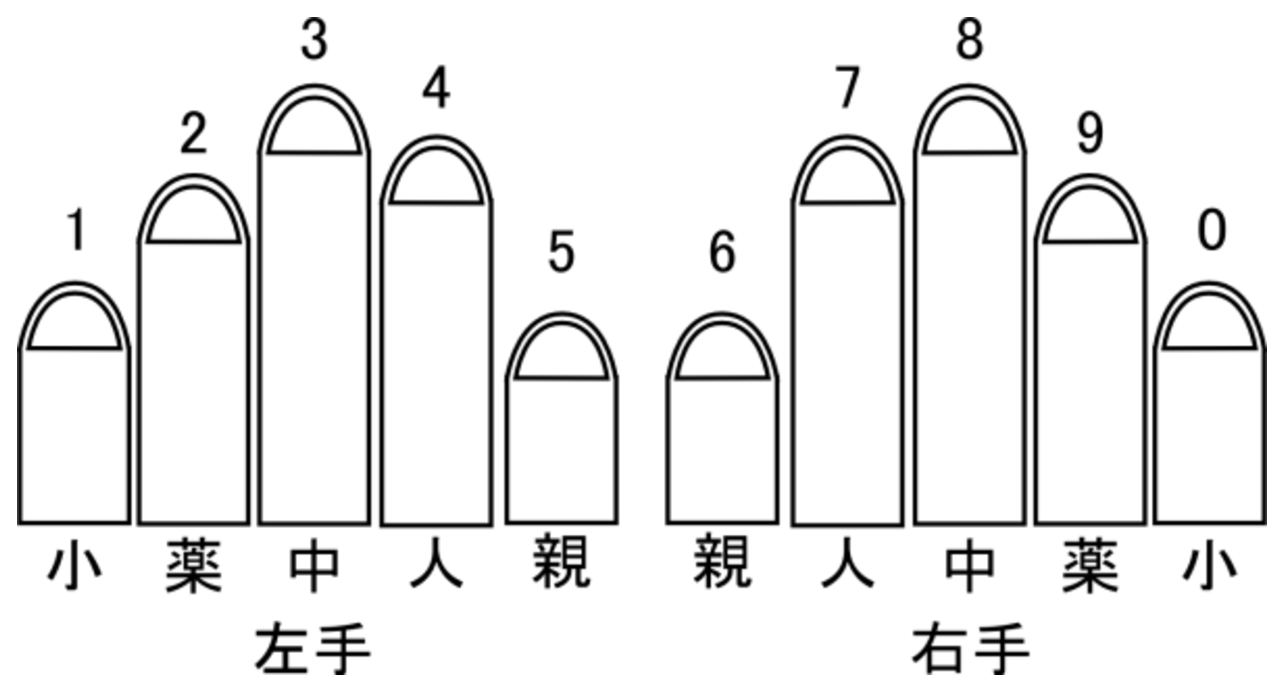
\includegraphics[width=13cm,clip]{res_tomoemon/finger.eps}
\vspace{-4mm}

\part*{意見と質問}
本書の執筆にあたってできる限りの確認をしていますが、誤字・脱字や誤解・混乱を招くような表現、内容が含まれている可能性があります。ささいなことでも構わないので気づいたことは執筆陣へご連絡いただけると幸いです。連絡は、本書の最後に載せている、執筆陣のtwitterやブログへお願いします。

\part*{謝辞}
本書の執筆にあたり、多忙なる中、快くインタビューにご協力してくださった、Pocariさん、dqmaniacさん、たにごんさん、むなしいさん、俺さん、Quvotaさん、父・信仁さん、あきうめさん、モルタルコさん、GANGASさん、えむさん、そして勃起教教祖さんに心より感謝いたします。特に、インタビューのセッティングからレビューの取りまとめに至るまで、窓口となって全面的にご協力頂いた Pocari さんには、格別の感謝の意を表します。執筆陣だけでは語ることのできない非常に密度の高い内容を盛り込むことができました。また、執筆陣の要望を聞いて表紙のイラストを描いてくださったcreamさん、サークル名を決める際にすかさず名前を挙げてくださったgummiさんに感謝します。その他、執筆陣へのご助力や宣伝にご協力してくださったみなさん、ありがとうございます。最後に、これまでタイピングに取り組んで様々な経験と知識を残してくださったタイピング界に関わるすべてのみなさんのおかげで本書は完成しました。本当にありがとうございます。



\clearpage

\tableofcontents

\clearpage

\thispagestyle{empty}
\section*{} % dummy

\clearpage
% 本文のページ番号はアラビア数字でここから1ページ目とする
\setcounter{page}{1}
\pagenumbering{arabic}

\articlepart{Typin' Girls - はじめての競技タイピング}{W/H}

\begin{screen}
過去の記憶がお前に喜びを与えるときにのみ、過去について考えよ。\\
―― Jane Austen
\end{screen}

\section*{序章}

\begin{verbatim}
「いつから」と問われれば、あの日を境に。
僕は君を見ることをやめた。
君と僕のつながりはそうして強まって。
その不可視の糸は、切れることなく今もつながっている。

見やりもせず一心同体となる、一見理不尽な関係が。
日々思い慕いながらも、打ちつけるという関係が。
声こそ聞こえなくても、姿こそ見えなくても。
日々の交流を通して深まってゆくのを感じる。

僕らの交流は、極めて物理的なものだ。
けれど、その実それは極めて言語的でもある。

――物理と言語の界面<インターフェース>。

喩えるならば、それは果てしない大河だろう。
そこに、気が遠くなるような労力をかけ、橋をかける。
決して彼岸に届くことはないと知りつつ、橋をかける。
そんな戯れが、今の僕らの交流の形だ。

とするなら、あの出来事は、七の並ぶ日の夜空のような奇跡だったのだろう。
僕と君が、出会った日を思う。

ふわり、耳元を春風が吹き抜けていった。そんな気がした。

季節は冬。
暖を取らねば震えるような気温の中、懐かしさとかすかな喪失感をも振り払うかのように、洗面器の湯に浸していた両手をタオルで拭う。

ゆるみきっていた姿勢を正す。目がさえる。
ほかほかと熱を帯びた手をそっと、あるべき位置に。
人差し指の腹で、小さな突起をそっとなでる。

意識を、肩に、腕に、手首に、指に、
――鍵盤<キーボード>に。
そして真っ白な雪原に踏み出すように、軽やかに、親指を弾ませた。

カタン。
新雪降り積む窓の外、記憶の扉の鍵<キー>の音。
\end{verbatim}

\section{実力チェック}
\begin{screen}
競えば伸びる。\\
―― Typing Attack の合言葉
\end{screen}

\subsection{タイピング極めました(笑)}

始まりは僕が高校に入った春のこと。

どうしようもないほど位相がずれたインドア青春を送っていた僕だったが、ジュニアじゃないハイスクールに来てとうとう部活というリア充感漂うものに入らなくてはならなくなった。必須だったのだ。

しかし幸いかな、僕にはパソコン部という預言されしメシアがついていた。他の文化部に目もくれず(運動部という存在は、全く、存じ上げません!)メシアに入部届を出した僕は、初日の部活動で度肝を抜かれることになる。

……悪い意味で。

\answer{おじいちゃん先生}{新入生のみなさん。パソコンを使うには、えー、この、キーボード、と呼ばれる、文字の、色々書いてある機械と、マウス、という、ネズミのようなかたt(ry}

\answer{僕}{(レベル低っっっっっっ)}

\answer{おじいちゃん先生}{まずは、日本語を、パソコンに、入力……入力というのは、えー……キーボード、を使って、タイピングを、やるわけですが……入力! この練習から、始めたいと思います。}

\answer{僕}{(トロい! トロイア! トロイア戦争!(←三段活用))}

\answer{おじいちゃん先生}{ローマ字は、みなさん、ご存じですか?}

\answer{僕}{(Yes, I do! 実戦(← 2ch やニコ動への書き込み)で鍛えてる僕に隙はなかった!)}

\begin{screen}
こんなレベルの授業や部活動が実際に行われているところもあるそうで。
筆者の経験では、大学の英語の講義で 2 回に渡り A-Z タイピングをやるだけだったなんてことが実際にありました。英語やろうよ英語……。
\end{screen}

そう、僕は中学の時に自分専用のパソコンを買ってもらって以来、自室で多くの時間をテラワロスなどと打ち込みながら過ごしてきた。タイピングのイロハなんて釈迦に説法。なにしろ僕は、すでにタッチタイプ(キーボードを見ないで打つ超クールなスキルさ)ができないこともない、というハイレベルに到達しているのだよ。

実際、先生の説明することはすべて事前に知っていることばかりだ。IME のオンオフ、ホームポジション、母音と子音、シフトキー……。

退屈すぎて、おもむろにブラウザを立ち上げクオリティを発揮しようかという考えが支配的になってきた……その頃、ようやく面白そうな話になった。

\answer{おじいちゃん先生}{では、もうタイピングができそうだ、という人は、デスクトップにある、この、e-typing という、えー……ボタン、じゃない、アイコン、をダァブル・クリック(←年配の方がカタカナ語を発音するとき特有のテンション)してみて下さい。}

\answer{僕}{(e-typing ……いつだったかちょっとやったことがあったっけ? まあなんとでもなるよ)}

\begin{screen}
スコア帯別のアドバイスが次章にありますので、読者の皆さんでパソコンが手近にある方は、ぜひここで実際に e-typing の「腕試し」に挑戦してみて下さい。\\
\url{http://www.e-typing.ne.jp/}\\
会員登録しないでもトップページから「ランキングタイピング」→「腕試しレベルチェック」と辿ればプレイできます(2011/11 現在)。もちろん会員登録して、ログイン後にプレイしても構いません。
\end{screen}

\answer{僕}{(今週のテーマは「元気が出る言葉」らしい。どんな文章だろう)}

\answer{僕}{(元気出るどころか、なんか、え、つらいけど……? あれ……涙が……?)}

\answer{僕}{(いやいや、集中だ。ザ・アンダーグラウンド・ネットワーク(←2ch やニコ動)で鍛えた秘められし力を解放するときだ……圧倒的スコアを\ruby{叩}{たた}き出せッ)}

カタ……カタ……カタ……。

僕の指先が光の速さで\ruby{迸}{ほとばし}った。\ruby{疾}{はや}い……圧倒的じゃないか我が軍は。

伸ばし棒 \key{-} や位置が悪い \key{B} \key{Y} を打つ所ではさすがに手元を見てしまうが、それ以外はほとんどタッチタイプ。僕のタイピングはタッチ時々チラ見、いいね、いい速度だよ!

\answer{おじいちゃん先生}{ほう! 君はすごいね、映画にでてくる、あれだァ、ハッカァ! みたいだね。}

\answer{僕}{い、いえ……別に……(おおおおおおい気が散るよ! あとちょっとなんだ黙って!)}

ピピッピピピッ。

\answer{僕}{(桂ァ、今何ミス!?)}

……。オツカレサマデシタ。

\answer{僕}{(終わりか……微妙だなぁ、誰かさんの妨害のせいで……)}

「腕試しタイピング」が終わり、結果画面が表示される。

\begin{figure}
 \begin{center}
   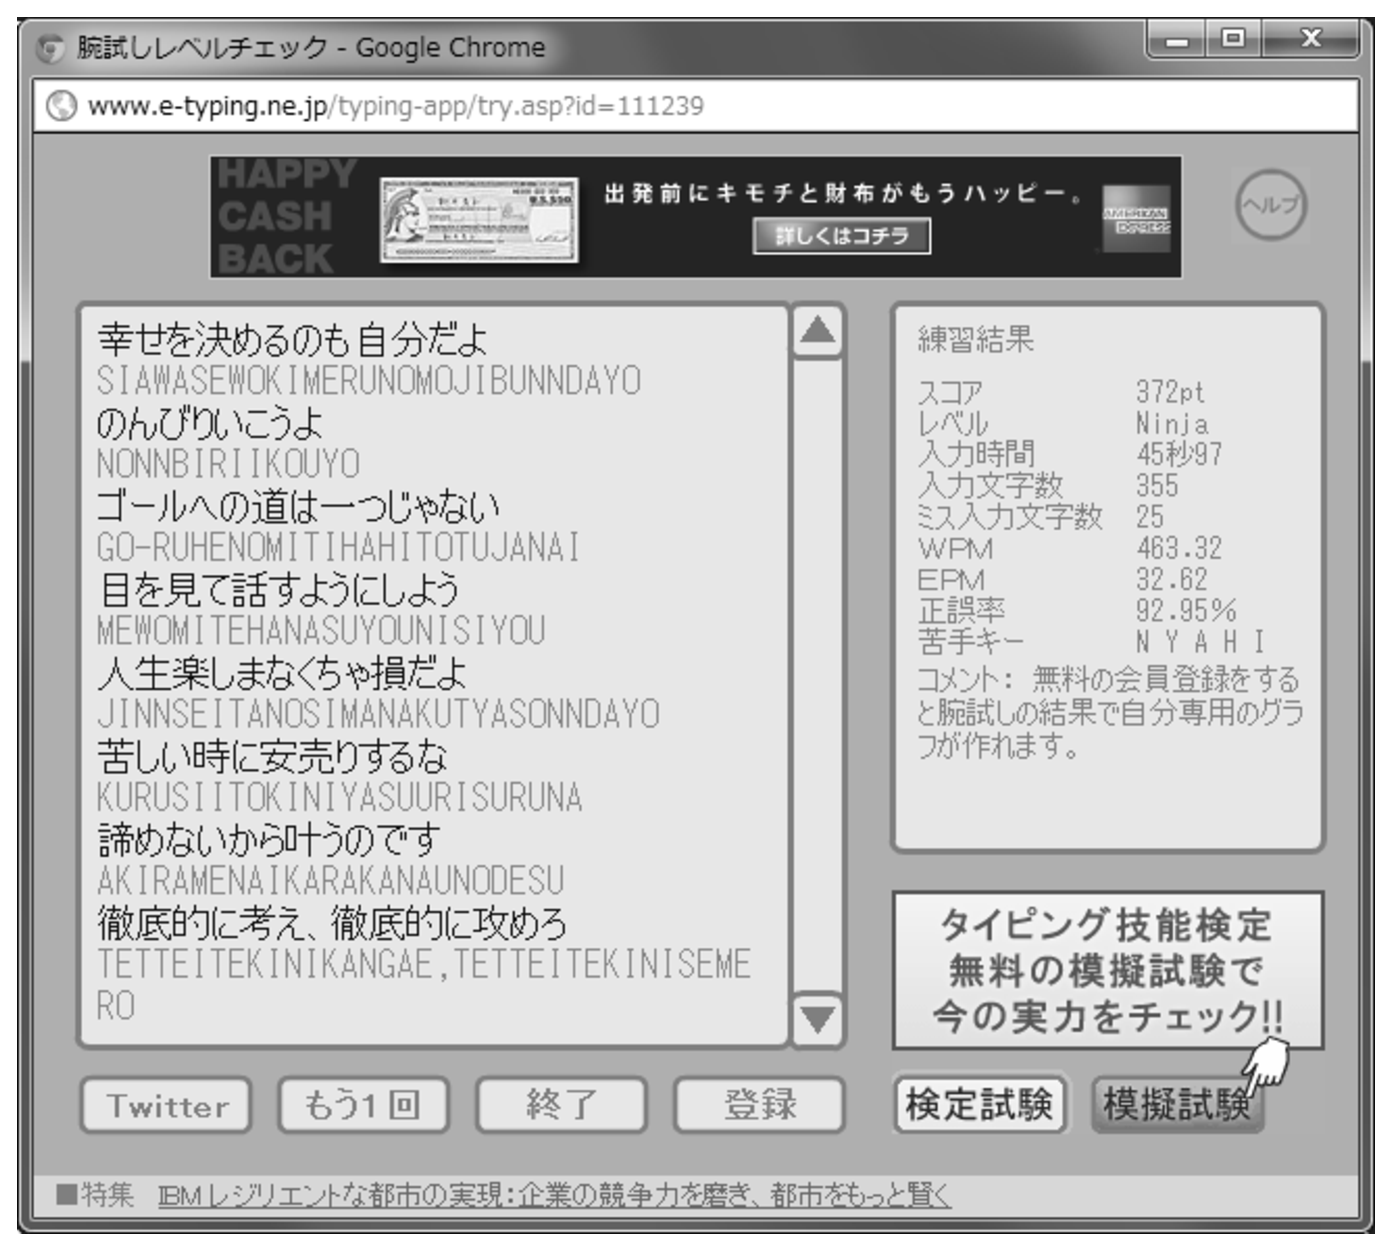
\includegraphics[width=7cm,clip]{res_x_i/ety_result1.eps}
 \end{center}
 \caption{e-typing結果画面}
 \label{x_i:ety_result1}
\end{figure}

\answer{おじいちゃん先生}{ニンジャ! ニンジャ、でましたよ! みなさん、372pt がでました。これはすごい、立派な記録ですよ。もっと速く打てた人、いませんか。}

\begin{figure*}
\begin{screen}
ここらで少々 e-typing について解説を。

最初に e-typing の紹介をしたのは、面倒な導入が不要で手軽にプレイして頂けて、かつ基礎的なタイピング力を見るのに適していると考えたためです。
e-typing の最大の魅力はユーザ数の多さで、ストーリーでもプレイしていた「腕試しタイピング」は毎週ランキングが更新されるのですが、各週のランキングに数千名が登録します。参加者数で見れば、間違いなく国内最大級のサービスです。
「腕試しタイピング」の他にも、入力する文章が様々に異なるモードがあります。「英語」や「長文」、「テンキー数字」など。
また同社が行っている「e-typing master」というタイピングの検定試験もあります。資格としての価値は正直なところあってないようなものですが、数少ないタイピング関連資格ではあるので、趣味でタイピングに取り組む際に目標のひとつにすると良いかもしれません(一番上の級「特級」は我々ガチ勢にとってもそれなりの難易度です)。

スコアについては、「僕」が 372pt で相当調子に乗ってますが、皆さんはどれくらい出るでしょうか。
ちなみに「僕」がプレイしていた「元気が出る言葉」という課題文のセットでは、全国ランキング登録平均スコアが 250pt 程度ですので、実際のところ「僕」のレベルはそれなりに平均以上ではあります。ざっくり偏差値で言うと 60 くらいでしょうか。

この記事は全体として、この時点における「僕」くらいの実力を持っている方を対象にして書かれています。つまり、タッチタイプが完全ではないにしろ\ruby{概}{おおむ}ねできて、実用上困らない程度には速く打つことができる人ですね。副題が「はじめてのタイピング」ではなく「はじめての競技タイピング」なのはそういうわけなのです。
したがって、タッチタイプがままならない方、とつとつとしか打つことができない方に対するフォローは残念ながら十分ではありません。このような同人誌に興味を持つ層であればまず問題ないラインと想定していますが、該当される方はごめんなさい。

なお、e-typing 攻略法については、まもなく登場するヒロインが、次章で解説してくれます。この章はほぼ伏線回収のための駄文だよ。やったね。
\end{screen}
\end{figure*}

だが周りの新入生はまだ黙々と、ピッピピッピと音を立てながら取り組んでいる。まだ打ち終わっていないのだ。

やや離れた所にいた、便乗して取り組んでいたらしき上級生の何名かも、見れば悔しそうな顔……。

つまり、僕の時代か。パックス・オレーノ、来ましたか。

\answer{僕}{ちょっと速すぎましたかね……。}

「ちょっとミスしすぎですかね」と言おうと思ったのに、つい本音が出てしまった。

だがしかし周りからは羨望の眼差し。冷静を装おうとするも、つい頬がつり上がってしまう。

\answer{おじいちゃん先生}{ニンジャ! 君のあだ名はニンジャね!}

\answer{僕}{(UZEEEEEEEEEEEEEEEE)}

こうして初回の部活動が終わった。成果は上々。

こんな感じでタイピングの神として君臨し、統治はせず、つかみはオッケーでゆるーく部活動を乗り切ることができるかと思うと、帰りの足取りは軽かった。というかスキップだった。

\subsection{タイピング界からの使者}

その日の夜、どこぞの運動部のように飯・風呂・寝るの確殺3連コンボを決めるわけがない僕は、帰宅後3秒で当然のように鞄から教科書を取り出し宿題と明日の予習を、やるわけもなく、パソコンの電源を入れ電脳空間へのダイヴ・フェイズへと移行した。

カスタムしてある愛機のログイン画面に、お手の物のタッチタイプでパスワードを\ruby{叩}{たた}き込む。パスワードのような、いつも同じ内容だと打つのがさらに速い。ダカダカダンとパワフルにマジカルにエクストリームに、

\answer{精}{いたたた! いたい、まだ用意できてないですし! ちょっと待っタンマ!}

どこからか声が聞こえた。

まあ、なに、珍しいことでもない。僕クラスになると想像力\ruby{逞}{たくま}しく幻聴が聞こえたりもするのだ。ラノベではないので驚いてやる義理もない。

スルーちからを発揮してダカダカダンとパワフルにマジカルにエクストリームに、

\answer{精}{痛いって言ってますよー無視しないでお願いあいたっ。}

今度は僕の目の前に――否、正確を期すれば、僕のキーボードの上に浮かび上がるように――確かに声の主らしきソレが現前した。

ソレというのはつまるところ、いやつまらなくても、このミニチュアロマン溢れる、ちんまいレディだ。年齢じゃなくてスケールがちんまい。何分の一フィギュアだ君は。

ちょうどキーボードのキーひとつの上に片足が乗るサイズの彼女は、どうも頭を打ったのか、セルフになでなでしながら表情を整えて、

\answer{精}{……ふぅ。気を取り直して、やっほー元気、はじめましてこんばんは。JST 的にこんばんは。}

どうしたことか、幻聴に続いて幻覚まで……などと認識否定を繰り返すのはまだるっこしく、僕もその手のフィクションでイラッ☆とする部分だ。

こんなこともあろうかと! 前々から万一自分の身に起こったらどうするかと、妄想もとい練ってきた策を発動する時がやってきた。僕はこの展開を自らの手で速攻、打破してみせる、速攻――即ちこうだ。

\answer{僕}{――君は霊か天使か女神か選ばれし現代人か異世界人か宇宙人か地底人か未来人か波動生命体か伝承存在か並行世界存在かメタ存在か妄想か脳腫瘍か視覚素子インプラントな拡張現実かオーパーツか人工知能高次元ホログラムか一体ナンデスカッ?}

はあはあと息が上がってしまったが、一気に言い切った満足感で(いやおそらくは酸欠のために)僕は言い知れぬ\ruby{恍惚}{こうこつ}感に包まれた。

そして気づく――死神とかダーク路線が手薄だ。

しかし、この光という光が泡立つ感覚の中魂どっきゅんと昇天するなら、それはありかナ――。

\answer{精}{タイピングの精です。かつタイパーです。typeする人でtyperと綴ります。英語的にはtypistが一般的とか言いっこなしで。}

なかなかやるな……平然と答えてきた。でも。

\answer{僕}{いや待った。自由解答じゃ困ります。上記の選択肢から選びなさい、複数選択可。}

\answer{精}{メタ存在と女神と未来人と並行世界存在と人工知能拡張現実と脳腫瘍がかすっていてあわせて 4 割、残り妄想という感じ? です。}

6割妄想かぁ! やっぱりね! 妄想に妄想ですと自己主張されるあたり、なるほど妄想じみている。

\answer{僕}{妄想メイン……じゃ害はないと? 危害を加える可能性しかないならご退散頂きたいし、危害あるかもだけどオイシイイベントもあるなら詳細聞くし、今すぐオイシイなら頂きますし、特に危なくもオイシクもないなら、自分の存在・文脈・世界設定について語れるだけ語っていって欲しい。僕がどうするかは、その後で決めよう。}

\answer{精}{適応力高すぎで私何も言うことないんですけど……その中では最後になりますか。オイシクなくてごめんなさい。オイシイのは厚くて熱いタイピング同人誌じゃなくて、薄いトリプルエックスなそれを別途お買い求め下さい。\footnote{この元ネタは gummi さんのツイートを参考にしました。勝手に加工・利用してすみません、感謝!}}

\answer{僕}{お買い求め? まあ、そのボディサイズじゃ色々あれだよね……(いや妄想メインならなんとでもなるんじゃ……いやまあ、設定を把握してからにしよう……)オーケー語って。}

\answer{精}{いいんです? ちょっと長くなるかもですよ?}

神妙な顔を作ってうなずく。僕の心が動かされれば、協力を惜しむつもりはない。

こういう不思議存在がコンタクトを取ってくる場合は決まって、何か困っているからだし。

\answer{精}{繰り返しになりますけど私、タイピングのアレです。ことタイピングに関してはエキスパートなタイパーのアレです。なんだっけ……精です、精。私に関して言えば、どこにでもいます。遍在してます。霊的なのです。えへん。で、今はキーボードの上に見えてますよね。半透明ですよね。これは\ruby{憑依}{ひょうい}的なアレで、この物理媒体と計算資源を通してあなたの認識に間接アクセスしています。ハイテクバイオです。えへん。この状態だとキーボードと一体化してるんで……こっちが準備してないのにダカダカと打たれると痛かったり。事実痛かったです。あ、もう大丈夫ですけど。それで、あなたと意思伝達ができてますけど……これは私の力だけじゃなくて、あなたと波長位相的なアレが合わないと無理です。だからあなたは選ばれし(というと聞こえは良いが要は妄想癖の)人的なアレで、ラッキーです。えへん、じゃないか、ぱちぱち。私の核というか本質はもっと抽象的で高次なアレですが、あなたの認識を必要とするという意味では属人的です。……これくらいで、私についてはわかります?}

\answer{僕}{組み合わせはわかった(←見栄)けど……その詳細が知りたいんじゃん。オーバーテクノロジーと証明可能な神秘学を手中に収め現代科学をあざ笑いたい。}

\answer{精}{はい無茶振り頂きました! っていうかそれやったらページ食い過ぎですから! 掘り下げたいのそこじゃないですから! ストーリーめちゃくちゃですから! ……はい、メタです。えへん。で、ですね……掘り下げたいのは「タイパー」の方なんですよう、私はタイパーの精なんですよう、「タイパーって何?」って聞いて下さいよう。}

\answer{僕}{(うわ……口が勝手に……)タイパーって何?}

\answer{精}{厳密な定義はない(諸派あって面倒です……)けど、ここではこう言っちゃいます。「タイピングを入力の手段としてではなくて、目的として行っている人たち」です。これくらい打てれば実用上十分……とかケチなことを言わないで、タイピングそのものを楽しみだしちゃったと。もっと適当に、「タイピングに情熱傾けちゃってる人たち」でも遠からずですね。そのタイパーの代表として私は来ました。すごい無理矢理がんばって、山ほど設定引っさげて、あなたの元へエッチラオッチラ(←こう書くとややエロい)やって来ましたんですよ。なので、言いたいこと言っちゃいます!}

ここまで聞いても、僕は彼女が言わんとすることが読めていなかった。

彼女が僕のタイピングに惚れ込んで、タイピングが世界を救うんだ宇宙で\ruby{隕石}{いんせき}を高速タイピングで打ち落とす人が必要なんだーとかいう話が出てきて、僕がヒーローになるというお花畑を幻視しているのみだった。

――だから割とショックだった。

\answer{精}{ええとですね、まずあなたは調子に乗りすぎなのです。の・り・す・ぎ・な・の・で・す! 井の中の\ruby{蛙}{かわず}です。凡百です。普通です。いや別に普通なのはいいです。でもそれで僕すげーって満足されちゃうと、私がむずむずします。黙ってられないです。世界を見せてやりたくなります。It's a typer world. ブルってる? と言いたいです!}

……何が何だか……わからない……。

タイピングなんかで凄まれる日が来ようとは。それも、こんなデフォルメチックミニチュアガールに。つついちゃうぞ?

\answer{僕}{つ、つまり、タイピングの精として、僕をパニッシュしに来た!?}

\answer{精}{別に罰しないですョ? タイパー優しいです。変人ではあっても愉快な人たちです。あなたはタイピングの基礎力もあって、人と競うことに価値も感じるタイプみたいなので、お仲間になれるんじゃないかなと思って。}

先ほどの凄んだ表情から、一転にこり。

つまりそれは勧誘だった。壮大な展開も、泣ける設定もなかった。

無論のこと、心など動かない。動きようもない。

……そんな風に思っていた時期が、僕にもありました。

\subsection{タイピング始めました}

想像できるだろうか。夕食を終えるなり両親との会話もそこそこに部屋に籠もり、(本人\ruby{曰}{いわ}く)半分オーバー妄想らしい存在と盛り上がる、(主に頭が)かわいそうな年頃の学生の姿を――僕である。

\answer{精}{お腹もふくれましたところで、現実を直視して頂きたいと思います。}

\answer{僕}{いや今というまさに今、妄想を、非現実を直視してるけど……。}

\answer{精}{\ruby{刮目}{かつもく}せよ! これが全・日・本レベル! 私の還る大・海・原! です! じゃん!}

\begin{figure}
 \begin{center}
   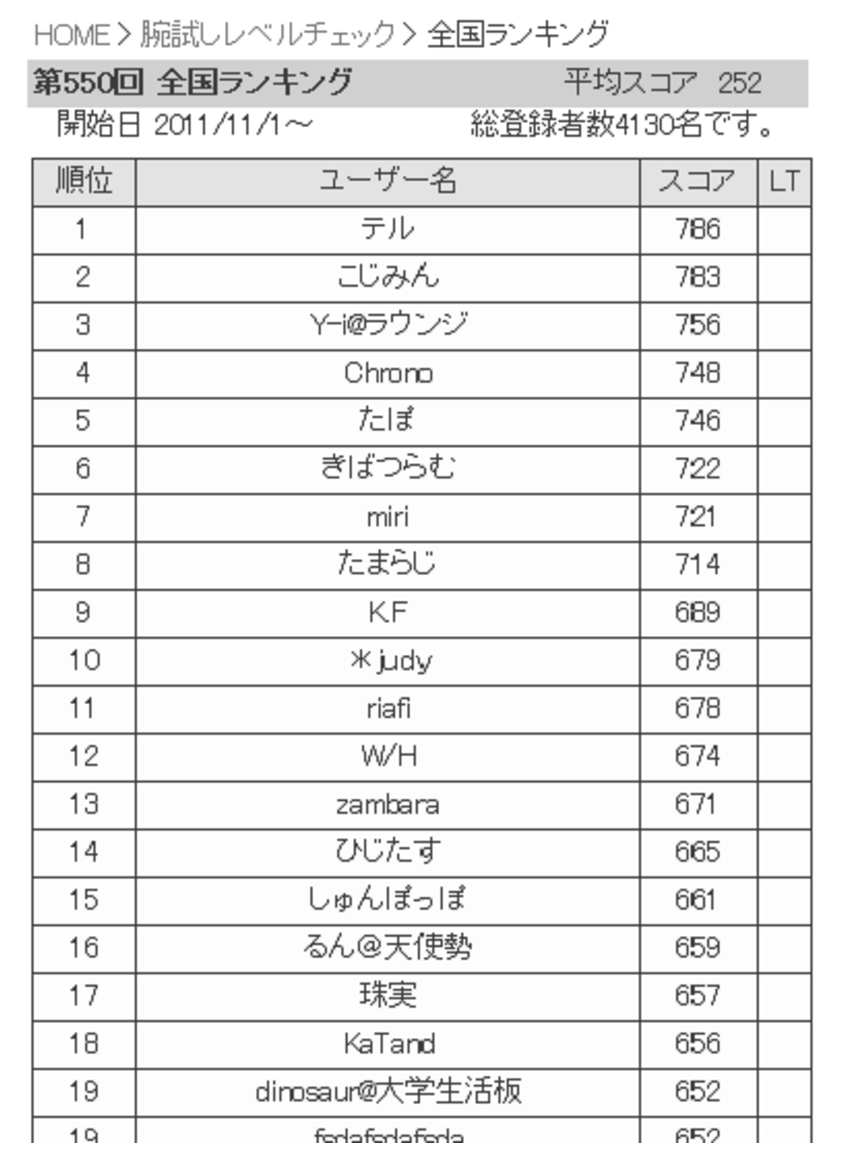
\includegraphics[width=7cm,clip]{res_x_i/ety.eps}
 \end{center}
 \caption{e-typing腕試し全国ランキング}
 \label{x_i:ety}
\end{figure}

\answer{僕}{えええええ!!(←約一名の自室に響き渡る近所迷惑な声)}

……ってなんすかこれ。一瞬でリアクションできる凄さ、どこにもないっていう……。テンション合わせてあげた僕、アホの子みたいっていう……。

\answer{精}{全・日・っp}

\answer{僕}{いやもうそのテンションいいんで、解説を。}

\answer{精}{はい。(←真顔)これは、学校であなたが打って 372pt を\ruby{叩}{たた}き出していた e-typing 腕試しモードのスコアの全国ランキングです。週ごとにリセットされるので、歴代のランキングとかじゃなくて、その週に出された記録しか入ってないですけど。}

\answer{僕}{わーすごい(←真顔)。チート使いばっかで荒れてる。}

\answer{精}{え、チート違いますよ?(←真顔)ガチですガチ。ガチタイパー勢です。}

\answer{僕}{いやだって……え?(←変顔) ウソでしょ? トップで 500pt とかだろ常識的に考えて……。}

一位のやつ、僕の倍以上スコアあるって?

大体、700 超えは若干名しかいないのに、600 後半はたくさんいるってのは……。

あれ? ってことは 600 後半の団子はガチってことに……いやいや 600 って…… 600!?

\answer{僕}{一位はチートじゃ? 「テル」って「チート」の変形もじりで自主申告してるし。}

\answer{精}{断じてチートじゃないですよう。現代の生きる伝説テル・ぶったーさんになんてことを……。}

\answer{僕}{え、でも……うーん……まあ、600 くらい出せる人がいるのはわかった。700 とかは眉唾かな。}

\answer{精}{(歴代トップだと 800 オーバーですけど……)いいでしょう、600。}

\answer{僕}{それくらいだったら、僕もやれば出せそうだけど。}

\answer{精}{今のままじゃ無理無理、絶対無理。っていうか、600 って私もそれくらいですし。}

\answer{僕}{え? そういえば君もタイパーって言ってたっけ。……出せるの? ってそのボディサイズじゃ無理じゃね?}

\answer{精}{見たいです?(←見せたくてうずうずしてる) 方法があるんですよー、これが。じゃあちょっと、お手をこちらへ。}

言うなり、キーボードの上からこっちこっちと手招く「精」(こいつ結局名前なんなんだ)。

先に説明すればいいものを、にこにこしたまま、黙って彼女は僕の手に触れシュイィーン! シュイィーンって!? シュイィーンって!!!

僕の肩から先の感覚はすぅっと、ろうそくの火でも吹いて消すかのように消えてなくなった。

\answer{僕}{ヴぁうおぁあああああああ腕がぁああああ! 僕の腕がぁああああああああああ!}

\answer{精}{あ、ごめんなさい。うずうずしちゃって説明が遅れました(てへっ)。こうやって\ruby{憑依}{ひょうい}すれば物理的に打てるなぁと……。}

見れば、確かに、腕は、ついている。

取れていない。痛みはない。

\answer{僕}{あああ……はうわっ、うおゎ、ぅわーお……(←目がマジ)。}

\answer{精}{一時的に借りてるだけですよ。ちゃんと戻せるし戻すので、そんなに焦らなくてだいじょぶです。目がマジにならなくてだいじょぶです。セーフです。}

\answer{僕}{お、オーケィ……。}

とは言ったものの、額には冷や汗が残る。いや、だってこれ、\ruby{憑依}{ひょうい}って……この感覚、普通じゃないよ。アブノーマルよ。妄想 6 割とか言ってたから油断しきってたっての……彼女の気分次第じゃ実害ありまくりじゃない。

だが当の彼女はというと、

\answer{精}{非ログイン状態でいっかー、おっけー、元気ワードね。実は長いだけで打ちやすさそんなでもないけど……ワード末尾の「できる」とかカモってるし、ま 600 は何度かやれば……!}

ノリノリである。本当にうずうずしていたらしく、僕はアウトオブ眼中。

\answer{精}{じゃ打ちまーす。}

感覚がない僕の腕から下が、僕の意識を通さず勝手にキーボードを操作していく。僕の手でありながら僕の手ではないという奇妙な体験。

この\ruby{憑依}{ひょうい}現象に文字通り全身全霊でびびって震え上がった僕は、彼女の気分を損ねないように、適当にスゲーとかヤベーとか言おうとヒヨっていて。

そして――言葉を失った。

ッタカタタタタタタタタタタタタタン!
ッタカタタ(ピッ)タタタタタタタタタタタタタタタタタタタン!
ッタカタタタタタタタタタタタタタタタタン!
ッタカタタタタタタタタタタタタタタタタタタタタタタタタタタン!
ッタカタタタタタタタタタタタタタタタタタタン!

音は弾倉交換しつつ撃ち続ける Machine gun なら、

手もコンピュータと同期し動き続ける Machine だった。

僕の手が勝手に動くという、恐怖感。僕の妄想でチートだろうという、非現実感。僕も何度かやればこれくらい出せるという、お花畑。それらがマシンガン音と残像の見えそうな指の高速移動に、撃ち抜かれ圧倒され吹き飛ばされる。

打ち終わって、一息ついたらしき彼女にかけるべき、いくつかの言葉が浮かんだ。

「ゴッデス! 君のあだ名はゴッデスね!」

「ちょっと速すぎますね……」

「Is it a typer world? 狂ってる……」

だけど、実際に口をついて出てきたのはこれだ。

\answer{僕}{タイピング、始めたいです。}

\begin{screen}
主人公と同じ気持ちになりたい方は、動画サイトにある高速タイパーのプレイ動画を見ましょう。
以下にいくつかおすすめのものを載せておきます。どれも魂が抜けるレベルです。

\begin{itemize}
 \item (ニコ動) sm8243869 あきうめ氏の「慣用句」798pt
 \item (ニコ動) sm13155297 あきうめ氏の手元
 \item \url{http://youtu.be/4YzFkzRbOcg} ひろりんご氏の「思い出の言葉」810pt
\end{itemize}
\end{screen}

\section{e-typingで基礎力を}
\begin{screen}
ミスをするくらいなら打つな!\\
―― 正確性重視を強調する、全日本タイピスト連合のキャッチフレーズ
\end{screen}

\subsection{敵を知り己を知らば}

無事に腕の制御を取り戻した僕は、早速彼女の話に耳を傾けていた。

\answer{精}{まずは姿勢です、そのやる気ない感じのそれをなんとかして欲しいです。}

\answer{僕}{なるほど把握、姿勢が重要なのは何やるにしても基本だね(シャキッ)。}

\answer{精}{いや現段階だと姿勢とか誤差です。}

\answer{僕}{と、言うと?}

\answer{精}{座学やるので、まじめに聞いて欲しかっただけです。}

\answer{僕}{あ、はい。}

\answer{精}{敵を知り己を知れば百戦危うからず! ……と偉い人は言いました。ということで、自分ってどれくらいの腕前だと思います?}

\answer{僕}{ふむ……けっこうすごいと思ってたんだけど。}

\answer{精}{そうです、けっこうすごいです、実際。}

\answer{僕}{こき下ろしたり持ち上げたり、どっちなん打!(あれ、なんだこのカンジ……)}

\answer{精}{一般人的には「すごい」んです。だって普段文字を入力するときに困ることなんてないでしょ? これなら。}

\answer{僕}{そういう意味じゃそうかな? ネトゲでチャットするのも、ブログ書くのも楽勝だしねぇ。}

\answer{精}{そう、普通にパソコンを使う時の入力手段としてなら、十分です。}

\answer{僕}{でも……さっきのあれ見ると、まだまだかなって。}

\answer{精}{ここから先は、言ってしまえば、基本的に遊びの領域です。文字の入力をお仕事にでもしない限り、見返りはあまりありません。だから「競技タイピング」と言っています。}

\answer{僕}{技を競うって書いて「競技」か……。}

\answer{精}{100m を 13 秒で走れる人が、がんばって 10 秒で走れるようになっても、そんなの日常生活ではほぼ何の役にも立たないですよね。でも陸上選手から見たら、その差はものすごいですし、10 秒で走れる人には賞賛が送られます。スポンサーもつくかもしれません。つまり陸上という世界の中では「10 秒で走れる」という、そのこと自体に価値があるわけです。私たちのいる競技タイピングの世界も、陸上と比べちゃうと小規模ではありますけど、そういう場所です。だからさっきは「井の中の\ruby{蛙}{かわず}」なんて言い方をしましたけど、井の中は井の中で快適です。困らないし、悪くないです。引き返すなら今のうち……ですよ?}

\answer{僕}{井戸ごと海に放り込んだのは誰ですかね……でも、いいよ。とりあえず君の記録はすぐ超えてみせるから。}

\answer{精}{わー、その意気やよし! やはり私の目に狂いはないですね。}

「役に立たない」と断言されて興味を失う人もいるんだろう。

でも、それを言ったら、僕の普段プレイするゲームだってそうだ。音ゲーがうまくても、FPS がうまくても、基本的に役に立たない。でも、楽しいからやる。

楽しいと思えるうちはやってみよう――それが僕の出した回答だった。

\answer{精}{では、仕切り直して、次は敵を知ります。解説のため、あなたが調子に乗りまくっていたニンジャ記録の重要部分をぺたっと。}

\begin{figure}
 \begin{center}
   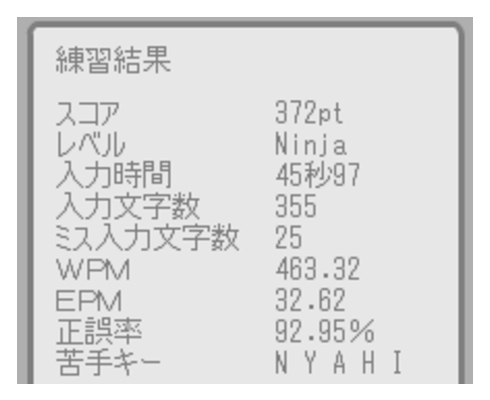
\includegraphics[width=7cm,clip]{res_x_i/ety_result2.eps}
 \end{center}
 \caption{結果画面の重要部分}
 \label{x_i:ety_result2}
\end{figure}

\answer{僕}{あれ、結果画面左の部分は見なくていいの?}

\answer{精}{左にはワードが並んでいるだけですからね、今は注目しないでいいでしょう。}

\answer{僕}{ワード?}

\answer{精}{タイピングゲームでの出題文のことです。英単語の word の意味通りに「単語」とは限りません。例えば、この e-typing なら、画面にひとつずつ文章が表示されますよね。この文ひとつひとつが{\bf ワード}と呼ばれます。まあ、ちゃんとした定義はなくて曖昧な感じですけど。ノリです、ノリ。}

\answer{僕}{なんとなく把握した。}

\answer{精}{ちなみに e-typing ではランダムに 15 ワードが出題されます。意味、わかりますよね。}

\answer{僕}{何か文章が表示されて、打って……と 15 回やったら終わりになる、と。}

\answer{精}{です。では各項目を解説しましょう。それぞれこういう意味です。}

\begin{itemize}
 \item スコア:結果から計算されたスコア。これで競う
 \item レベル:スコア帯に応じた称号
 \item WPM:一分間に何回正しいキーを打つスピードか
 \item EPM:一分間に何回ミスをするペースか
 \item 入力時間:入力を受け付ける状態だった総時間
 \item ミス入力文字数:ミス(誤打鍵)をした回数
 \item 入力文字数:正しく打った文字の数
 \item 正誤率:1 - ミス入力文字数 / 入力文字数
 \item 苦手キー:ミスが多かった部分のキー
\end{itemize}

\answer{精}{まず WPM が一番注目したくなりますね。}

\answer{僕}{タイピングの速度か。僕は一分間に 463 回、ってことは 60 で割れば……一秒間に 8 回弱。やっぱかなり速いよね。}

\answer{精}{ですね。最初は秒速に直して考えた方が大体のスピードがわかりやすいはず。でも、タイパーの人達は分速の方に慣れてます。その方が整数で表現できたり、大きい数になるので差がわかりやすかったり、メリットがあるので。まあ心配しなくても、多くのソフトでこちらが使われているので、そのうち分速の方に勝手に慣れますよ。}

\answer{僕}{EPMはWPMのミスタイプバージョンか。}

\answer{精}{正直なところ、あまり注目することはないですね。というのも「ミス入力文字数」も表示されるので、普通はこっちに注目します。}

\answer{僕}{これは単にミス回数だよね。}

\answer{精}{そうですけど、「何カ所でミスをしたか」ではないことに注意です。同じ部分で何回も間違ったキーを押すと、一回ずつこの「ミス入力文字数」にカウントされちゃいます。}

\answer{僕}{何回「ピッ」ってなったかってことね。「入力文字数」は……正しく打った文字の数ってことは、出題されたワードによって決まってくる数。}

\answer{精}{ほぼその考えで合ってますけど、実はちょっと違います。が、これはディープな話なので後回しで……「入力時間」「正誤率」についても、なんとなくで大丈夫です。}

\answer{僕}{「苦手キー」は間違って押したキー?}

\answer{精}{ではなくて、ミスをした箇所で押さなきゃいけなかったキーです。あなたの記録の場合\key{N},\key{Y},\key{A},\key{H},\key{I}を押さなきゃいけない場所でミスが多かったというわけ。}

\answer{僕}{レベルはスコアで決まるんだよね。最高のレベルまではやりたいところ。}

\answer{精}{その発想は……フフフ、危ないかと?(暗黒微笑)そしてお待ちかねのスコア計算式ですが、こうなってます、ででん。}

\begin{screen}
スコア = (WPM - EPM) $\times$ 正誤率の二乗
\end{screen}

\answer{僕}{へぇ。WPM - EPM が 430.7 だから、これに 0.9295 を二回かけて……372.111986675。確かにスコアの 372pt に合うね。}

\answer{精}{ここからわかることはなんでしょう?}

\answer{僕}{うーん……スピードが速いとスコアが高くなる。}

\answer{精}{当たり前すぎますけどね。……むしろ、速度である WPM をベースに、そこからしょっ引かれていくという見方が重要かな。もし引かれなければ、WPM がそのままスコアになるわけです。}

\answer{僕}{EPM が 0 で正誤率が 100\% なら、WPM がそのままスコアか。それってつまり……一回もミスをしないってこと。}

\answer{精}{Exactly(その通りでございます)。EPM も正誤率も、ミスに関係した数ですからね。ミスをすると EPM が増えて正誤率も下がる。しかも正誤率は二乗で計算されちゃうので……イメージとしてはミスのペナルティが三重につく感じです。三重苦です。}

\answer{僕}{この記録 25 回もミスってるじゃん(主に誰かのせいで……)、もしこれがなかったら、WPM がそのままがスコアで、463pt!}

\answer{精}{ミスが多すぎます。はじめからやり直してください。ミスをしないということは、ミスをしたことに気づいて打ち直す……っていうタイムロスもなくなるということです。だから今のあなたの場合、実はノーミスなら WPM も上がる余地があるってこと。}

\answer{僕}{500pt 完全に見えたよ、これ。}

\answer{精}{さあ、それはどうでしょーかね?}

キーボードの上に陣取る妄想生命体(なのか?)は、謎の笑み(=暗黒微笑)を浮かべるとそう言い残し、姿を消した。僕の目の前には、明け渡されたキーボード。

よし、やってやろうじゃないか。500pt の壁、速攻打破してみせる。ミスをしなければ大丈夫だ、問題ない。

\subsection{何戦してもまだ危うい}

それから数日が過ぎた。

あの日はどうも疲れていたようで、あれ以来、腕の感覚がなくなることも、おかしな幻覚・幻聴を体験することもなくなった……という展開になる可能性を 50\% 程度と想定していた僕だったが、現実は妄想に寛容だったらしい。今日も、部屋には打鍵音が響き渡っている。

\answer{僕}{……(ピッピッ)くそ……またミスって詰ま(ピッ)ってミス(ピッ)って詰まって……(ピピピッ)うううう!}

未だに 500pt を出すことはできていない。それどころか、450pt すらも出ていない。

\answer{精}{急ぎすぎなんですよ。}

\answer{僕}{でも、このスピードじゃないと……何度もやれば 500pt が出るはずなんだよ。奇跡が起きれば。}

\answer{精}{気持ちはわかりますけど、さすがに絶望的です。そろそろ気づいてるんじゃないですか? ある程度スピードを落とさないと、ノーミスなんて出ないって。}

\answer{僕}{ノーミスならスピードも伸びる余地があるって言ったの君だ! だまされた! うぼぁー!}

\answer{精}{言いました。言いましたが、今回すぐそれが達成できるとは言ってません……つまり、達成は 10 年後、20 年後ということも……。}

\answer{僕}{ひょおおおおおおおお!}

\answer{精}{という冗談はさておき。}

\answer{僕}{はい。(←ノリに慣れてきた)}

\answer{精}{エンジン全開で打って、運良くミスがなかったら……なんていう妄想的な打ち方をしていると e-typing は永遠に、アレです、クソゲーです。イライラ棒です。だからその逆、ミスを極力しないような打ち方で、どれだけスピードを出せるか、と考えるといいです。}

\answer{僕}{やってみるか……。}

\answer{精}{プレイ中に\key{Esc}キーを押すとプレイ中止、結果表示画面で\key{R}キーを押すとリトライできるので、活用してください。}

\answer{僕}{いや、それ最初に言ってよ……。}

―― 十数分後 ――

\answer{僕}{やっと出たし……ノーミス。}

\answer{精}{めでたいです。スコアは……。}

\answer{僕}{340pt。ダメじゃん! 最初の記録よりも下がってる! ゴミ過ぎる!}

\answer{精}{ミスをしないように打つのがいかに難しいか、わかったんじゃないですか。滅茶苦茶に乱打してノーミスなんて奇跡は、まずないんです。}

\answer{僕}{悔しい……けど感じちゃう……その通り。ミス数を抑えようとして打つと、すごく遅くなる。ビクビクして、速く打てないっていうか……。}

\answer{精}{(この歳にしてこのネタ根性……)でも、そこで無理して指を動かすと、ミスになっちゃいますよね。}

\answer{僕}{それそれ。でもじゃあ、速くてノーミスって……どうやるの?}

\answer{精}{魔法のような解決策はないです。でも、練習をすると、だんだんできるようになります。さっきも言った通り「ミスをしない範囲で速く」という意識でタイピングをすることは重要です。今はノーミス縛りでやってもらいましたが、必ずしもノーミスである必要はないですよ。はじめはミス 3 回までとか、それくらいを意識するだけでも十分、効果があります。}

\answer{僕}{そんなこと考えてタイピングをすることなんて、普通ないしね。}

\answer{精}{普段のタイピングシーンでは「適当に速く打ってミスしたら直す」か「速度は気にせず、丁寧にゆっくり打つ」かどっちかなんです。「速くて正確ぅ!」\footnote{元ネタは「バトル&ゲット! ポケモンタイピングDS」。}できれば最高なんですけど、なかなかそれは意識しませんよね。}

\answer{僕}{それを目指すなら、初心にかえって練習あるのみってことか。}

\answer{精}{そう。そしてそういう意味で「速くて正確ぅ!」なクールなタイピングの基本を身につけるには、e-typing のスコアルールは割と、ちょうどいいんです。ノーミスで打ってさえいれば伸びるというわけでなし、ミスを増やしてでも速く打てば伸びるというわけでなし。両立ができた時、良いスコアが出るようになっています。もちろん、運の要素もありますけどね。そこはゲームですから。}

\answer{僕}{意外と奥が深いから困る。}

\answer{精}{この程度で奥が深いなんて言っていたら……気絶しますよ?}

\answer{僕}{楽しみにしとく。}

と言ってしまってから、本当に楽しみにしている自分に気づく。

この時の僕は、わかったようでいて、何もわかっていなかったのだ。踏み込もうとしている世界が、一体どのような魔境であるのかすら。

\subsection{段階別攻略}

僕は正確性を重視して練習を重ね、とうとう 3 ミス 440pt という記録を出すに至った。ミスがなければ 450pt 超え。悔しさはあったが、もう 450pt は時間の問題だと確信できる。

そして同時に、500pt を改めて意識する――。

\answer{僕}{一番いい助言を頼む。}

\answer{精}{いろいろな要素がありますからね……段階によって大まかにアドバイスになりそうなことはありますが、個人差もありますし。読者さんのこともありますので、段階別に色々と見てみましょか。}

\subsubsection{~200pt}

\answer{僕}{じゃ、100pt とか 150pt とかの雑魚は?}

\answer{精}{言い方はどうかと思いますけど……でもごめんなさい、そういう方には練習してくださいとしか。パソコン入門的な本や初心者向けのタイピング練習サイトを参考にするのもいいですし、別に参考にしなくても、ひたすら打っても伸びる頃だと思います。e-typing にも「腕試し」の他に「基礎練習」「基本練習」のようなコンテンツがあるので、試してみるのもいいですね。}

\answer{僕}{キーの位置を覚えたり、ホームポジションからの動かし方を練習したりするやつね。}

\answer{精}{面白みがあまりないので軽視されがちですけど、伸ばし棒\key{-}や\key{P},\key{Z}みたいな小指の方にあるキーと、あと人差し指で幅広くカバーしなきゃいけない中央付近のキーは、後々まで苦手意識が残りやすい部分です。もっと速く打てている人でも、不安があったら良い機会だと思って練習しましょう。}

\answer{僕}{さすがに僕にそれは当てはまらないな。(←ハイフンのたびに減速してる人の台詞)}

\subsubsection{200pt~300pt}

\answer{僕}{250pt くらいが一般の人の平均らしいけど、このへんは?}

\answer{精}{そうですねぇ、例えば「き」なら右手中指で\key{K}\key{I}という風に打ちますよね。こういうひらがな単位での運動は、反復練習して無意識にできるようにすることが大事です。別にまだキーボードを見ていてもいいので、無意識に、ひらがな単位でまとめて。}

\answer{僕}{250pt もあれば、それはとっくにできるんじゃ?}

\answer{精}{かもです。個人差があるって言葉でお茶を濁します。ひらがな単位でまとめて打てるなら、今度は単語とかのレベルの「まとまり」を意識して練習するといいです。}

\begin{screen}
\begin{itemize}
\item[ ] みかんをたべる
\item[×] み/か/ん/を/た/べ/る
\item[○] みかん/を/たべる
\end{itemize}
\end{screen}

\answer{精}{このように認識しやすい単位に分けて、各部分はスムーズに打てるように。最初から「たべる」の 6 打鍵 TABERU をまとめては難しいかもしれません。その場合は TABE で 4 打鍵とか、もう少し細かく分けた所からスタートでもいいでしょう。ひらがな単位よりは長い部分を一気に、というのがポイントです。}

\answer{僕}{e-typing を始める前から気づいたらやってたな。}

\answer{精}{ある程度速く打てる人は、必ずこうやっています。できるようになると一気に速くなりますね。}

\answer{僕}{他には?}

\answer{精}{このスコア帯の人に限らないですが、ここから先は「もっと速く打とう」と意識して打たないと伸びていかないと思います。実用的な目的でタイピングをしている人などは、この程度のスピードでも特に不自由しないので、「タイピングとは、これくらいのスピードで考え、指を動かすもの」って速度の制限を無意識にかけてしまっていることがあります。もっと速くなりたいなら、ハングリー精神を持ちましょう。大丈夫、あなたの限界は全然こんなところじゃないです。}

\subsubsection{300pt~400pt}

\answer{僕}{300pt 以上ってなると……練習を始める前の僕くらいか。じゃ、この間言われたことの通りなのかな。}

\answer{精}{そうですね。タイピングに特化した練習はしたことがないけど、パソコンはバッチリ! 系の人はこの辺じゃないでしょうか? 繰り返しになりますが、焦りすぎず、正確性重視で打ってみることをオススメしたいレベルです。初めからノーミスなんていう人は少なくて、400 WPM 以上出ているけど、ミスのペナルティのために 350pt 程度、という人が多いですし。}

\answer{僕}{僕もそのタイプだったわけだ。あとこれさ、やっぱり慣れもあるよ。ワードの種類ってそんなに山ほどはないから、何度も何度もやってると打ち方がわかってくる。}

\answer{精}{週ごとにワードのお題、ワードセットが変わりますが、各セットは 100 から 500 種程度のワードからなってます。多いと思うかもですが、打っていればすぐ見たことのあるワードばかりになっちゃいます。ワードごとの癖が把握できていれば、もちろん打つのも速くなりますし、スピードを出せるワードはどれか、ミスしやすいワードはどれか、なんていう意識・調整もしやすいわけです。そうやって慣れることを{\bf ワード慣れ}と言っていて、もちろん重要ですね。}

\answer{僕}{それでけっこう伸びた感じがする。}

\answer{精}{ひとつ前で解説した、まとまりで認識、ということに関連して、{\bf 先読み}と呼ばれる技術もそろそろマスターしたい頃です。}

\answer{僕}{あーあ、イケてる名前の技が出てきちゃいましたね……僕の時には言わなかったくせに……。}

\answer{精}{いじわるじゃないですよ? あなたの場合は最初からできていたのです。名前は荘厳ですけど、実は大したことじゃないので。常に今打っているところの少し先にまで目をやってワードを読んでおいて、打鍵が途切れないようにする技術のことです。}

\answer{僕}{それかぁ……確かに最初からできたよ。}

\answer{精}{e-typing のように文章形式でワードが出てくる場合は、先読みが特に簡単ですからね。別の競技だとワードが単語単位だったりするので、その場合はまたちょっと訓練が必要です。}

\subsubsection{400pt~500pt}

\answer{僕}{やっと今の僕のレベルだ。}

\answer{精}{一般人的速いライン 400pt から、タイパー的 500pt の壁まで……色々な攻略が考えられる時期です。一つには後半加速という要素が大事になってきます。各ワードのはじめの部分は、まだ速く正確に打つのが難しいと思います。でも、後ろの方は頑張ると速く正確に打てるはず、という考え方です。}

\answer{僕}{どうして後ろは速く打てるわけ?}

\answer{精}{詳しくはまた改めて解説しますが……「各ワードの打ちはじめの所が難しい」というのは実感しませんか?}

\answer{僕}{確かに、はじめの数文字で急ごうとするとミスになることが多いか? 手を急に動かすのがキツいのかな。}

\answer{精}{それもありますけど、ワードが表示された瞬間は、そのワードが一体どういう文章なのか? 最初の文字は何か? とかで頭がいっぱいじゃないですか。でも、後ろの方を打つ頃には、先読みをしていれば、もう頭の中でワードが読み終わっているので。}

\answer{僕}{打つことに専念できるってことか。}

\answer{精}{はい、とりあえずそういう理解で良いと思います。ワード慣れとも関係しますね。何度も何度もそのワードを見て打ったことがあれば、より一層読む必要がないじゃないですか。百人一首で、上の句の途中まで聞いただけで、下の句まで全部わかってしまうような感じで。}

\answer{僕}{ちょっとわかる。}

\answer{精}{このあたりからは、やり込んで体で理解しないと、頭だけじゃわからないかもしれません。他にもワードをまたぐ際のリズム感ですとか、ワード慣れを徹底して加速できるワードでは攻めていくとか、言えることはありますが……どれも説明だけで理解するのはキビシイんじゃないかと。そういう意味で 500pt あたりに壁は実際にあると思いますです。}

\answer{僕}{基本的には実戦あるのみか。}

\answer{精}{e-typing だけで 500pt 以上まで鍛えようとするのは、正直つらいかも。次章以降で紹介する他のソフトも使ってベースになる速度を底上げしつつ、目標のひとつとして取り組むのがおすすめですね。逆に言えば、基本的な速度が十分あって、正確に打つこともできるなら、e-typing に特化した練習はしたことがなくても 500pt は出せます。}

\answer{僕}{じゃあ、500pt より上の世界は?}

\answer{精}{競技タイピングに特化した練習をしたことがないのに 500pt なんて人はほとんどいません。だから、ほぼ全員タイパーの世界ですね。やっほーみんな見てるー? 晴れ舞台だよー! と言いたいです。}

\answer{僕}{とか言ってごまかして、教えないつもりでしょ。}

\answer{精}{入門者に語るような話じゃないと思って、遠慮しただけですよ? でも興味があるなら……ついでに紹介しちゃいましょう。あなたはその方が燃えるタイプみたいですし。}

\subsection{行きすぎた攻略}

キーボードの上に鎮座していた「精」は立ち上がると、僕に背を向けて大きく呼吸した。これからすごいことを語るよという、要らない演出だ。

\begin{screen}
しかしこの節は、脅しではなく本当に敷居が高いです。
自信のない方は飛ばして読んだ方が、むしろスッキリするかもしれません。
ストーリー的にも何も進展はないので、気軽に飛ばしてください。
\end{screen}

\answer{精}{まず、ここから先のレベルを目指すには基本的な打鍵速度も絶対に必要です。反復練習も必要になりますし、攻略法を知っただけでどうこうなるものではないです。}

それは、450pt 目前まで取り組んだ僕もすでに感じていることだった。自分を鍛えないとどうしようもない。攻略法のような情報は、そのための道しるべでしかない。

\subsubsection{ワード先頭部分の高速化}

\answer{精}{ここまでのレベルとの最大の違いは、いわゆる初速と呼ばれる要素が重要になってくる点です。「はじめの部分は速く打てない」とさっきは諦めたようなことを言いましたが、そこを切り崩さないといけません。最初の一打までにかかる時間が短く、かつ最初から最高速で打ち始めるのが理想です。}

\answer{僕}{最初の一打までの時間……?}

\answer{精}{はい。私は{\bf レイテンシ}と呼んでいます。この時間のこと自体を{\bf 初速}という人もいますね。この要素の重要性については、こういう図を書くとわかるんじゃないでしょうか。e-typing の慣用句というテーマに「\ruby{匙}{さじ}を投げる」というワードがあって、私が打つとこんな感じの結果(図\ref{x_i:ety_bar})になります。}

\begin{figure*}
 \begin{center}
   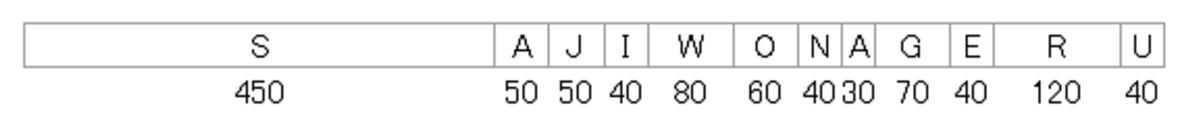
\includegraphics[width=14cm,clip]{res_x_i/ety_bar.eps}
 \end{center}
 \caption{文字ごとの打鍵時間}
 \label{x_i:ety_bar}
\end{figure*}

\answer{精}{見方はわかりますよね。各文字を入力する際にかかった時間が、その部分の横幅に対応しています。数字の単位は ms(ミリ秒、1/1000 秒)ですね。}

\answer{僕}{最初の\key{S}でかすぎだろ、常識的に考えて。}

\answer{精}{初めのキーは\key{S}じゃなくても、どんなキーでもこういう結果になります。打鍵速度が遅いうちは気になりませんが、後ろの部分の打鍵速度がこれくらい速くなっていると、むしろここが重要というわけです。}

\answer{僕}{450ms って……これはどうなの? 遅い方?}

\answer{精}{これも個人差がすごくあるんですが、特に訓練をしていないタイパーで 450ms から 500ms 程度だと思うので、並ですね。今のあなたのレベルだと……平均 500ms 以上はかかるかな。}

\answer{僕}{……でもこれは 100ms とかには絶対ならないよね。反射神経的にさ。}

\answer{精}{訓練すると、平均 400ms に持っていくことは誰にでもできると思います。そして初速・レイテンシを重視して記録を出しているトップランカーともなれば 350ms 程度がバシバシ出せます。数字だと僅かな差に見えるかもしれませんが、ワードが短いと、これだけで 50pt とか 100pt とかの点差につながります。さっきの図、再度凝視してみて欲しいです。後ろの部分はかなり極まってます。ここを速くして 50ms 縮めるのは厳しい。でもレイテンシなら、それくらいは削る余地があります。}

\answer{僕}{もしレイテンシが 350ms になれば全体で 100ms 分短くなるから……割合で見ても相当速くなるね。どうやったら鍛えられるの?}

\answer{精}{一番重要なのは{\bf ローマ字読み}と呼ばれるスキルを身につけること。「\ruby{匙}{さじ}を投げる」の方ではなくて、「SAJIWONAGERU」というローマ字表記された方を読み取って打つんです。}

\answer{僕}{なるほど、「\ruby{匙}{さじ}」を読むのにかかる時間がもったいないってことだ。「S」ならそのまま \key{S} って打てる。でも、一打目はともかく、その先までローマ字読みで速く打てる気はしない……。}

\answer{精}{はじめからローマ字読みをしていたという人もいますけど、訓練で後から身につけることもできます。一朝一夕には無理ですけどね。初めだけローマ字読みして、ワードの半ばからは漢字かな交じり文の方を読む人もいますし。}

\answer{僕}{今すぐは手がでないな……他には?}

\answer{精}{反射神経を鍛えるため、右脳的なトレーニングをすることも効果がありそうです。瞬間的に判断する脳の働きを鍛える感じでしょうか。}

\answer{僕}{それは才能というか、生まれつき決まってるんじゃ……?}

\answer{精}{「反射神経」と言うと、そういう神経があって、生まれつきみたいに思っちゃいますけど、生物学的にそんな神経はないですし、陸上選手だって卓球選手だって、後天的に鍛えてますよね? 才能のような要素がゼロだとは言いませんけど、そう言って逃げちゃうのは最後の手段。まず努力して、考えて、工夫して、また努力して……その後の話です。}

ジーザス、久しぶりに目が怖かったので、僕はそこで納得して、この話はもう持ち出さないようにしようと密かに誓った。

\subsubsection{ワード末尾部分の高速化}

\answer{精}{初めの部分がボトルネックなら、最後の部分は攻める場所です。}

\answer{僕}{後半加速が重要、ってのはさっきも言ってたけど?}

\answer{精}{もっと加速するのです! ワードとワードの間に、休み時間がありますよね。だから、各ワードを打ち切る最後の部分ではかなり無茶な打ち方をしても体制を整え直せる。それを利用して、ワード末尾はあとのことを考えず、手首や腕の動きも使ってドカンと一気に打ち込む……{\bf スパート}と呼ばれたりしますね。}

\answer{僕}{言ってる意味はわかるけど、感覚的にはさっぱりわからない。練習しようもない。}

\answer{精}{ですよねー(←やや嬉しそう)。まあ、基礎能力が一定レベルになったら感覚的に納得できます。その時に使うかどうか検討してください。}

\subsubsection{入力文字数の水増し}

\answer{精}{あとは、レイテンシの話とも関係して、ワードの長さ……結果画面でいう「入力文字数」を増加させる裏技的なテクニックがあります。}

\answer{僕}{前にディープだから後回しって言ってたね。裏技って何事……。}

\answer{精}{e-typing は柔軟にローマ字入力を受け付けてくれるので、わざと打鍵数が多くなるような打ち方をするんです。比較的簡単なのは「し」の \key{S}\key{H}\key{I} や「う」の \key{W}\key{H}\key{U} でしょう。過激なところでは「い」\key{Y}\key{I} や「っ」\key{L}\key{T}\key{U} のようなものまで使う変態もいないことはないです。}

\answer{僕}{\key{W}\key{H}\key{U}なんて、その入力自体初めて知ったっていうレベル。}

\begin{screen}
いっしょう\\
ISSYOU\\
YIXTUSHILYOWHU
\end{screen}

\answer{精}{この例は極端ですが、打鍵数が倍以上になっています。}

\answer{僕}{打鍵数が増えると何か得だっけ? スコアは WPM を元にするから、速度が速くないと意味ないんじゃ。}

\answer{精}{そこでレイテンシが関係するんです。ワードが長くなればなるほど、レイテンシによるタイムロスを後ろの部分の高速打鍵で補うことができますよね。}

\answer{僕}{ん……うーん?}

\answer{精}{「うし」を \key{U}\key{S}\key{I} って 400ms で 3 打鍵できますか?}

\answer{僕}{まず無理……レイテンシだけで 450ms とかになるって言ってたし、その時点で僕には無理。}

\answer{精}{6 打鍵の \key{W}\key{H}\key{U}\key{S}\key{H}\key{I} を 800ms ならどうです?}

\answer{僕}{最初の \key{W} が 450ms くらいで、残りが 350ms ……厳しそうだけど、無理ってほどじゃないのかな。可能性は見えてる。}

\answer{精}{計算するとわかりますが、どちらも WPM は 450 になります。後者の方が楽ですよね。}

\answer{僕}{WPM は「速さ」だから、「道のり」(打鍵数)と時間が両方倍になっても変わらないってことね。}

\answer{精}{{\bf 水増し打鍵}と呼ばれています。わざと長くなるような打ち方をするというのは、タイピングを入力の手段として見ると本末転倒なので、賛否両論ありますし、効果も微々たるもので使わない人も多いですが…… e-typing をゲームとしてみた時にはこうした攻略もあるということです。}

\answer{僕}{ぐぬぬ……。(←気絶寸前)}

\subsubsection{どこまで行っても正確性}

\answer{精}{もちろんですが、以上のような非常に高度なことを行いつつ、正確性は維持しなきゃダメです。打ち始めを高速化し、隙あらば長くなるような打ち方で打鍵数を稼ぎ、各ワード末尾では瞬間的にものすごく加速しながら、ミスはできるだけしない。このような戦いになってきます。}

\answer{僕}{す、数ミスなら問題ないんじゃなかった……?}

\answer{精}{このレベルになると、そうも言っていられません。スコアの計算式、覚えてますか?}

\answer{僕}{WPM から EPM をひいて、正誤率の二乗を……。}

\answer{精}{「かける」。そこが曲者です。スコアが割合で減っちゃうわけです。WPM の 5\% が減らされるとして、WPM が 400 なら 20pt ですけど、WPM が 800 だと 40pt 減ります。}

\answer{僕}{40pt は痛いってレベルじゃないね……ちょっとミスをしただけで、致命傷なんだ。}

\answer{精}{目指すのはあくまでノーミスです。結果的に 1 ミスか 2 ミスくらいで良い記録になることもありますけど。数ミスなんてしちゃったら、基本的にダメですね。}

\answer{僕}{うーん……ちょっと……見えない世界だ……。}

\answer{精}{はい、どう見ても喋りすぎました。今の時点ではこういうことは全然意識しなくて大丈夫。忘れておいて、頃合いになった時にでも、ふと思い出してくれれば十分です。}

どこまでも空は\ruby{禍々}{まがまが}しく、そして\ruby{艶}{あで}やかに\ruby{煌}{きら}びやかに VIP クオリティさえ包括するレベルを目の当たりにし、全力で頭が痛くなった僕は、その日は練習もそこそこに、e-typing 腕試しのランキングを眺めて寝た。

\section{Weather Typing と最適化}
\begin{screen}
もうあの記録が破られることは絶対に無いでしょう。\\
――あきうめ、自身の TOD 日本記録を振り返って
\end{screen}

\subsection{タイピングのモデル化}

その翌日。いつものように昼食を終えるなり図書室に駆け込んでパソコンスペースを占領し画像検索を始めようとした僕の前に、ヤツがにょろっと現れた。

キーボードの上に現れるメカニズムは未だによく解明されていないが、このシュールな光景にもだいぶ慣れつつある。

\answer{精}{暇ですねー。}

\answer{僕}{いや君やることないの!? っていうかずっとストーキングしてるの!? っていうか学校でまで独り言つぶやかせたいの!?}

\answer{精}{タイパー志望ってことは、変態志望みたいなものですからね。}

\answer{僕}{いやこれは変態っていうか変質者だから!}

\answer{精}{さておき、e-typing 練習を通して、とにかく指を速く動かすことができればタイピングが速い、なんてことはないと痛感したことと思います。}

\answer{僕}{あーもう、いきなり説明に入っちゃったよこの人……。}

\answer{精}{人じゃなくて精なんでー。……そんな運動能力のようなものは、一要素に過ぎない。あんだすたんです?}

\answer{僕}{そりゃまあ、指を速く動かすだけなら、こうやって、がちゃがちゃがちゃって適当に打てばめちゃくちゃ速いもん。でも実際はこのスピードでは打てない……ワードを読んで、正しく打たなきゃいけないから。}

\answer{精}{実はその「読む」「打つ」をもっと詳しく掘り下げたモデルが考えられていますので、ここで簡単に解説したいと思います。この先の話をするのに便利なので。}

\answer{僕}{モデルとかリア充は爆発してよ……。}

\answer{精}{「モデル」というのは目に見えないようなことを説明しやすくするために、考え方に簡単な形を与えたもの……のことです。まず、タイピングをする際に行われているステップを大きく三つ、{\bf 認識} {\bf 組立} {\bf 動作}に分解して考えます。}

\answer{僕}{ちょっと待った。僕は今、子守歌を四時間にわたって拝聴し、お腹の中を山の幸で満たし、四月の陽気に包まれて、この静かな図書室で香り立つようなふかふかのソファーに全体重を預けている。君の解説を聞いて、寝ないことがあるだろうか? いやない。}

\answer{精}{意外と寝ないと思いますよ。むしろ e-typing で苦労した経験のある今のあなたにとっては、エキサイティングなはず。}

\answer{僕}{やれやれだぜ……。(←眉につばをつけている)}

\answer{精}{全力で腰を折られたので再掲しますと、{\bf 認識} {\bf 組立} {\bf 動作}に分けます。第一のステップは「認識」です。ワードを視覚などでとらえて、今から打つべきはどういう文章なのか、と把握するところまでです。}

\answer{僕}{「読む」と同じ?}

\answer{精}{大体そうでしょう。ただ、音を聞いて打つタイピングゲームがあったとすると「読む」では不適切なので、「認識」という言い方になってますね。}

\answer{僕}{それじゃあ、僕の言う「打つ」は「動作」か。}

\answer{精}{そこが難しいところです。「動作」はもちろん、指を実際に動かしてキーを打ちに行くことなんですが……ここで質問タイム。「認識」でどういう文を打つかが判明した時点で、「動作」できますか?}

\answer{僕}{できそうな気がするけど……そんなこと聞くってことはできないんでしょ。三つのステップってさっき言ってたし。}

\answer{精}{……ひきょうものぉ……。でもその通り。「認識」だけでは、どういう文字の並び({\bf 文字列})をこれから入力するか、ということしかわかりません。「動作」するためには、どのキーを打てばいいか、そのキーは物理的にどこにあって、どの指をどう動かせば打てるか……そういうこともわかっていないとだめですよね。そのイメージの集まりに{\bf 打鍵列}と名前をつけます。}

\answer{僕}{「動作」は本当にただ動かす部分だけなんだね。その直前の、どのキーをどの指で打つのか、みたいなイメージ……打鍵列だっけ。それを作る部分は別に必要だと。}

\answer{精}{はい、そのステップの名前が「組立」です。実際に打つイメージを頭の中で組み立てるという感覚ですね。このステップは、ほぼ無意識に行われていることも多いかと思いますが、競技レベルになると必要に応じて意識する必要があります。「認識」「組立」「動作」。こう説明すれば、自然な分け方だと思いませんか?}

\answer{僕}{まあ……(いいように誘導されてる気がするけど)そうかな。僕たちは実際こういうステップで打ってるってこと?}

\answer{精}{厳密な意味では、違うでしょう。脳とか神経とかのレベルに分解すれば、本当はもっと山のようにステップがあるはずで。ただ、私たちにとってちょうど考えやすく、それなりに細かく分析もできるので、今はそういうものだと思って考えましょうというお話です。}

\answer{僕}{まだ全然、どう役に立つのかわからないよ。}

\answer{精}{個々の要素を説明してる段階ですからね……最後に合わさると、すごいです。もうひとつだけ下準備をさせてください。{\bf バッファ}というものを導入します。}

\answer{僕}{(ややカッコイイのが出てきた……)}

\answer{精}{難しい単語に見えますが、大したことはないです。上にも下にも栓がついているペットボトルを考えてください。上から水を入れると中に水が溜まり、溜まった水は下の栓を開けると外に出すことができる。そういう一時的に水をためる装置にバッファという名前がついていると思えばいいです。}

\begin{figure}
 \begin{center}
   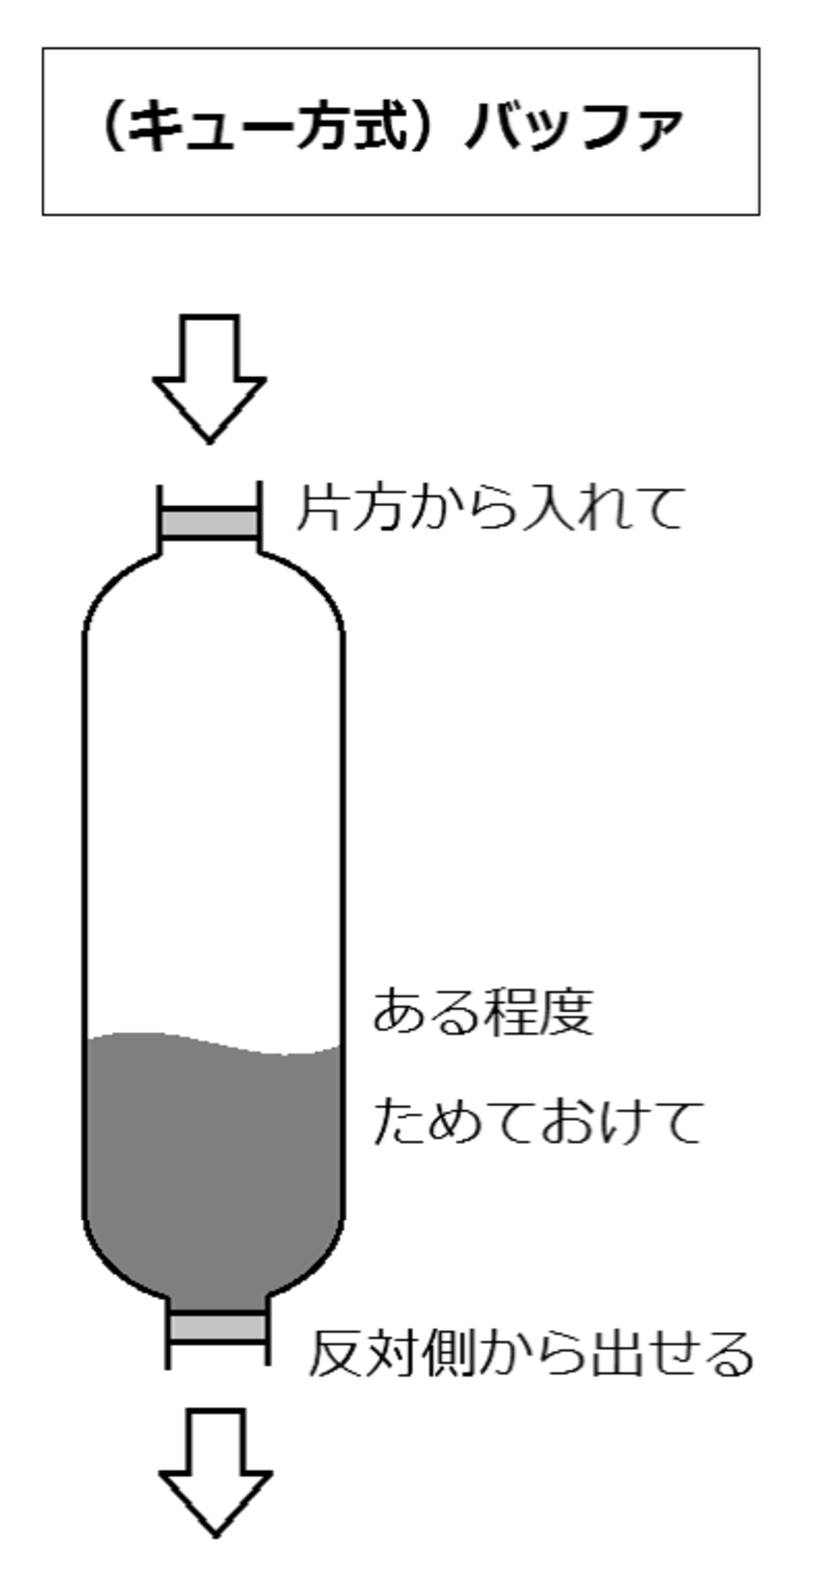
\includegraphics[width=7cm,clip]{res_x_i/model1.eps}
 \end{center}
 \caption{バッファ}
 \label{x_i:model1}
\end{figure}

\answer{僕}{どういうものかはわかったけど……これ何の役に立つの?}

\answer{精}{例えば、上からちょっとずつ入ってくる水をしばらくためてから、一気に下の栓をあけてドバァってやるとか。こういう装置がないとできないですよね。}

\answer{僕}{まあ、そうだけど……。}

\answer{精}{逆に一気に上からドバァって来たのをためておいて、後からちまちま出して使ったり。そういう風に、出し入れの速度を調整するために使えます。}

\answer{僕}{まだ微妙だけど……名前がカッコイイから許した。}

\answer{精}{実際に使われているところを見た方が早いですね。このモデルでは、バッファを縦に二つ、連結します。図をどうぞ。}

\begin{figure}
 \begin{center}
   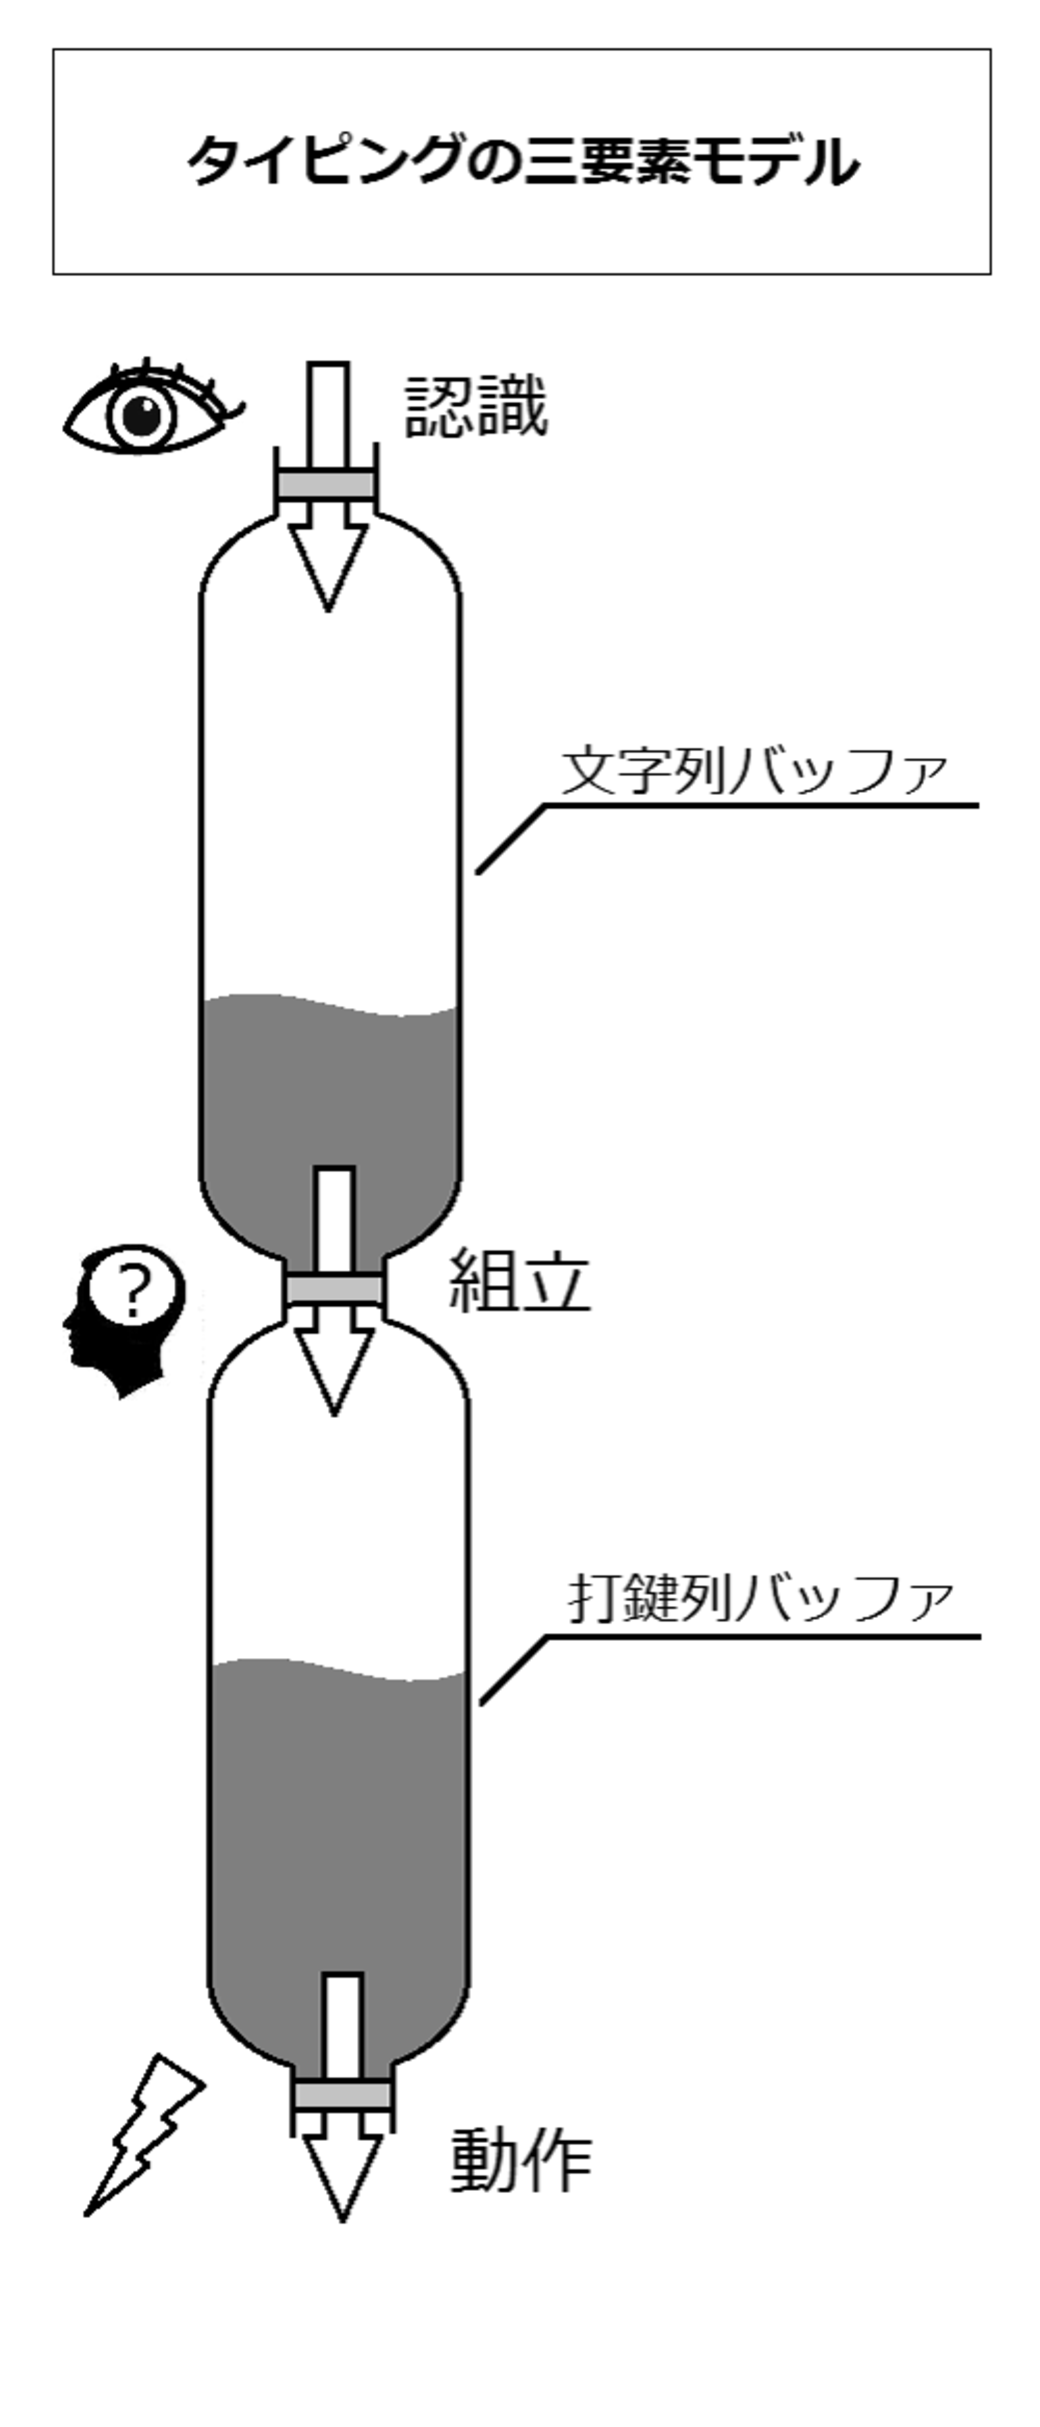
\includegraphics[width=7cm,clip]{res_x_i/model2.eps}
 \end{center}
 \caption{タイピングの三要素モデル}
 \label{x_i:model2}
\end{figure}

\answer{僕}{(連結した!?)}

\answer{精}{図を見てもらえばだいたいわかっちゃうと思いますが……まずワードを「認識」すると、こういう文字列だなという理解が、上の文字列のバッファにたまります。}

\answer{僕}{まだ「文字列」だから、どう打てばいいかってことはイメージできてないわけだね。}

\answer{精}{そうです。「認識」しただけでは打てないので、続けて「組立」です。文字列バッファに溜まっている水(文字列)から一定量取り出して打鍵列を「組立」するわけですね。できた打鍵列が下の打鍵列バッファに溜まります。}

\answer{僕}{おお……。}

\answer{精}{打鍵列が完成したらめでたく「動作」できます。つまり「動作」では打鍵列バッファから水(打鍵列)を取り出して、実際の打鍵を行うことになるわけです。どうですか!}

\answer{僕}{バッファの役割がわかった気がする。}

\answer{精}{大事なポイントとしては、「認識」「組立」「動作」はそれぞれ順番に行われるわけではなくて、同時並行的に進めることができるってことです。}

\answer{僕}{それぞれの栓を同時に水が通過していけるイメージね。}

\answer{精}{そして私たちがやっている競技は、このモデルで言うと、ワードという一定量の水をこの装置の上から注ぎ込んで、どれだけ早く一番下まで\ruby{濾過}{ろか}完了するかという勝負なわけです。}

\answer{僕}{今まで「読む速度が遅い」と言ってたのは「認識」「組立」部分の栓が細いってことで……「打鍵するだけならいくらでも速くできる」って言ってたのは「動作」の部分の栓は他と比べると太いってことだ。}

\answer{精}{考察しやすそうでしょう? e-typing でワードの初めの部分で急ぎすぎるとミスしやすいという話がありましたが、あれは「認識」「組立」が追いついてなくて打鍵列バッファが空なのに、無理に「動作」しようとしたからなんです。}

\answer{僕}{早すぎたんだ……打鍵列が腐ってやがる、と。モデルがあると便利ってこういうことね!}

\answer{精}{これからは、このモデルの理解を前提に話をしますね。}

\subsection{動作がネックになる時}

帰宅後、早速今日得た情報を使って e-typing を攻略しようとしたところ、タイピングの妖精さん(←そういうことで妥協したらしい)に止められてしまった。

\answer{精}{せっかく三要素モデルを紹介したので、「動作」の部分がつらいケースも知って欲しいのですよ。}

\answer{僕}{「動作」は大丈夫だ問題ない、でファイナルアンサーなんじゃなかったっけ。}

\answer{精}{e-typing に取り組む分には、まだしばらくそうです。でも世の中には他の競技種目となるタイピングゲームもあるので。そろそろ他のものも紹介したいと思って。}

\answer{僕}{ぶっちゃけ e-typing のミス音と血しぶきに殺意を感じ始めてたから、嬉しいな。}

\answer{精}{Weather Typing というのが「動作」の限界を感じるには良いので、ダウンロードしてきて下さい。}

\answer{僕}{インストールは僕に任せろー! ……オーケー、あとは WeatherTyping.exe を起動して、と……「シングルプレイ」でいいの? ってか対戦もあるんだね。}

\answer{精}{対戦についてはここでは詳しく解説できないですけど、よく出来ていて楽しいですよ。Weather Typing に慣れてきたらぜひ挑戦してみてください。}

\begin{screen}
Weather Typing\footnotemark

本当はネット対戦がアツくてメインなソフトなのですが、この記事ではシングルプレイに限定した書き方になっています。
対戦にも興味を持たれた方は、上記ページの「その他」→「ロビー」→「参加方法」を参考にロビーに入って常駐するといいでしょう。
ただ最近は常に人がいるという状態ではないようなので、友達を誘うと確実です。
\end{screen}
\footnotetext{\url{http://denasu.com/software/weathertyping.html}}

\begin{figure}
 \begin{center}
   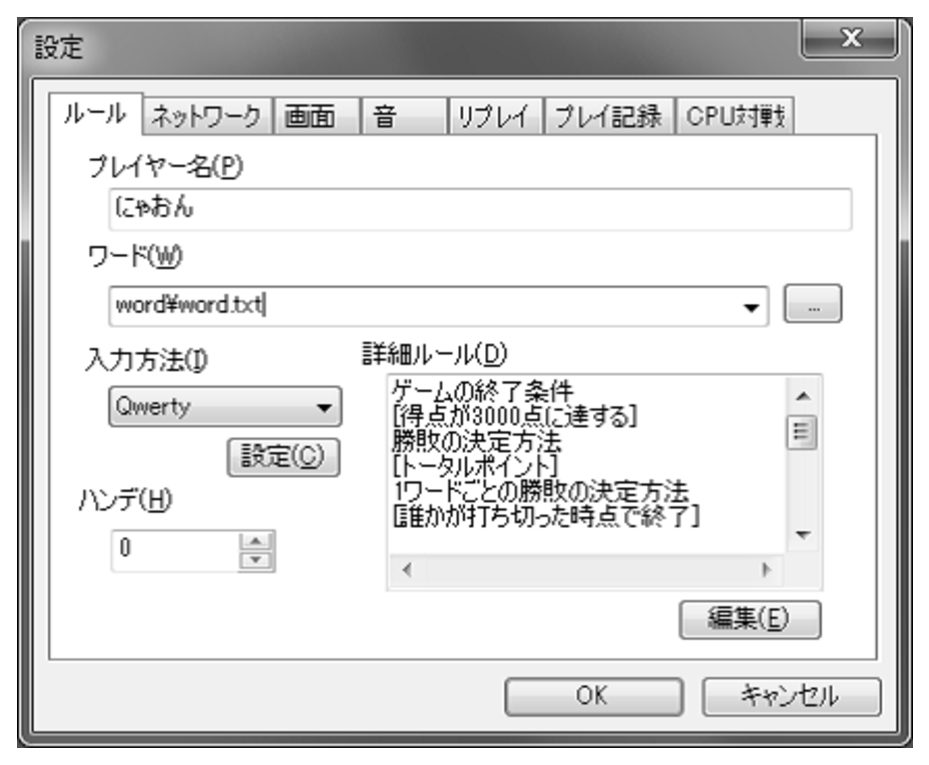
\includegraphics[width=7cm,clip]{res_x_i/wt_setting.eps}
 \end{center}
 \caption{Weather Typing 設定画面}
 \label{x_i:wt_setting}
\end{figure}

\answer{僕}{たくさん設定項目が出てきたけど……。}

\answer{精}{かなり細かく設定ができるんですけど、重要なものはあまり多くないです。今はとりあえず「ワード」とある欄でワードファイルを指定できるということだけ覚えておきましょう。}

\answer{僕}{ワードを自分で作れるんだ。}

\answer{精}{e-typing に慣れていると新鮮ですよね。だから e-typing のワードで練習したいものだけ集めてきて Weather Typing で練習したりなんてこともできます。今はデフォルトのワードファイル word.txt のままでやってみましょう。}

\begin{screen}
独自のワードファイルは直接テキストファイルを編集して作るか、Weather Typing 本体に\ruby{同梱}{どうこん}されている WordMaker.exe を使って作ります。
WordMaker.exe を使えば簡単に作れますので、一度やってみることをおすすめします。
\end{screen}

カタカタカタ。

基本的には e-typing と同種のゲームという感覚だ。画面にワードがひとつずつ表示されて、打ち終わると次のワードに行く。独特のワードに所々つまずきつつも、順調に打つ。……やや長い。

\answer{僕}{……終わった。Complete 30、Speed 510、Accuracy 92 で、Total が 46920。}

\answer{精}{結果の解説は要ります?}

\answer{僕}{いや、もう大体わかる…… Complete はワード数、Speed は e-typing の WPM と同じ意味で、分速何打鍵か。Accuracy は正誤率。Total がスコアでしょ。}

\answer{精}{ばっちりです。ちなみに Total は Speed かける Accuracy で計算されてますよ。}

\answer{僕}{e-typing はスコア計算でミスが三重ペナルティだったから、それに比べるとミスのペナルティは小さいな。}

\answer{精}{Weather Typing の方がスピード重視ですね。ですが、Weather Typing でスコアアタックをする際に一番大切なポイントは、そんな部分じゃないんです。}

\answer{僕}{一番大切なポイント……(ごくり)。}

\answer{精}{Weather Typing では、e-typing の章で解説した初打までの時間「レイテンシ」が、なんと計算に入りません。}

\answer{僕}{計算に入らない? ……ワードが表示されてから、ゆっくり考えて打ってもいいと?}

\answer{精}{イエス。なので、基本的な部分では e-typing に対する攻略が流用できますけど、上級レベルになると e-typing とは別ゲーになります。何しろ短いワードなら最初にじっくり見ておくことで「認識」「組立」を完全に完了できます。つまり打鍵列バッファが満タンの状態で、あとは「動作」だけという所からスタートして競えるわけです。}

\answer{僕}{どれだけ指を速く正確に動かせるかって勝負……。}

\answer{精}{このように打鍵列を十分に組み立ててから一気に打つことを、{\bf ため打ち}と言ったりしますね。}

\answer{僕}{ゲーム的で面白そう。}

\answer{精}{もっと面白くするために、このワードファイルで打ってみるといいです。}

\begin{screen}
ダウンロードして頂けるようにワードファイルを置いておきます。\\
\url{http://dvorak.jp/archive/bura.txt}

Weather Typing のフォルダ内にある word というフォルダの中に保存し、Weather Typing 起動時の画面でこの bura.txt を選択すると使うことができます。

ちなみに、以下の 20 ワードが入っています。

あみあみ かにかに きらきら くいくい\\
くらくら こうこう これこれ さくさく\\
ざわざわ たじたじ ぬくぬく ぬるぬる\\
ふらふら ぶらぶら ぶんぶん ちょこちょこ\\
ぽきぽき むんむん ほげほげ しゅいしゅい
\end{screen}

\answer{僕}{いかにも打ちやすそう……しかも、考えてから打ってもいいと来た。いくらでもスピード出せるでしょ!}

\answer{精}{そう思いますよね。でも実際は……ま、いつものパターンです。}

\answer{僕}{そうわかっていても、突撃するのが僕だった! スタート、っと。}

「くらくら」……えーと\key{K}\key{U}\key{R}\key{A}……楽勝。「さくさく」……楽勝。「ぶんぶん」……人差し指が……。「むんむん」……うーん、きつい。「ざわざわ」……フォオオオ!

\answer{僕}{…… Speed 670。ワードが短いし、レイテンシ無視で考えてから打てるから、さっきより断然速くはなってる。けどワードによっては全然だめだったな。「むんむん」とか。}

\answer{精}{「ぶんぶん」「ぬるぬる」「むんむん」「ぬくぬく」あたりは右手の人差し指を酷使するワードですね。}

\answer{僕}{そいつらはまだいいとして……「ぽきぽき」「ざわざわ」は指がつるかと思った。これが「動作」がボトルネックになる感覚……。}

\answer{精}{その一部ですね。これだけお膳立てすれば「認識」「組立」が十分なレベルでなくても、「動作」もいずれ問題になりそうだということが体感できたでしょ。そして、もっと速くなると e-typing のような競技でも、部分的にボトルネックが「動作」になることはよくあります。}

\answer{僕}{「動作」は物理的な指の動きだから……指を鍛えたりすれば伸ばせるよね。}

\answer{精}{頑張って競技タイピングをやっていると、タイピングに関しては、どんどん指が器用になっていきますね。キビキビと正確に動くようになります。}

\answer{僕}{今までは先読みだとかノーミス意識だとか、脳トレ的な話ばっかりだったけど、筋トレ的な要素もちゃんとあるんだね。}

\answer{精}{タイピングは頭も身体も使う万能競技ですよ。ダイエットにも(多分少しは)なります。}

\answer{僕}{手とか指しか動いてないけど?}

\answer{精}{それでも、二、三時間も本気で打てば汗だくになれます。それくらい激しく「動作」できるくらいに、他の部分が速くなってからの話ですけどね。}

\answer{僕}{タイピングで汗だくは想像したくない……。}

\subsection{打ち分け・最適化}

何度も例のワードファイルで Weather Typing を打っていると、どんどん指の動かし方に慣れてきた。速いワードはとことん速く、遅いワードも詰まらないように。動作部分の訓練は、どうやら僕に向いているらしかった。

\answer{僕}{よし! Speed 750 突破ッ!}

\answer{精}{わあけっこうすごいですねー(←上から目線)。}

レイテンシを無視しているとはいえ、e-typing で 750pt といったらトップレベルだ。これくらいのスピードで e-typing のワードを打ち続けることができれば、750pt ……!

僕はタイピングを始めてから最大級の胸の高鳴りを覚えていた。

だから、こんな挑発をしてしまう。

\answer{僕}{ヨウセイサァン、余裕じゃないっスか……これの記録どんだけなんスかぁ?}

\answer{精}{私ですか?}

\answer{僕}{そっスよ……最初の一回 e-typing 見せてもらってから全然手本見せてくれないじゃないっスか。}

\answer{精}{それは……教育上よくない理由がありまして。でも良い頃合いですね。見せましょう。多分、2000 とか出ますけど。}

\answer{僕}{2000!?}

さすがに冗談だと思った。

―― 二分後 ――

\answer{僕}{ォオオオオオオオオオオオオ!!!}

ワードが爆風に飛ばされるように消えていく……。まさに瞬殺。打ち始めたと思った直後には、すべて打ち終わって、消えている。

そして彼女に乗っ取られた僕の手が、僕の指が、変な方向に曲がって奇妙な動きを見せている。なんだこれは! 大丈夫なのか!? 異次元パワー\ruby{炸裂}{さくれつ}しすぎだろ常考ッ……!?

\begin{screen}
ワードは違います(この動画の方が遥かに高度です)が、参考動画をどうぞ。
ひろりんご氏の独自ワード Speed 1905 Accuracy 100\\
\url{http://youtu.be/jf9kArBHQvE}
\end{screen}

そして打ち終わる。

\answer{精}{……うーん…… Speed 1700 でした。残念、2000 行かなかったですね。まあ「ざわざわ」出すぎでした。運ゲー運ゲー。}

\answer{僕}{ちょ、ちょっと……これは\ruby{卑怯}{ひきょう}っスよ先生……異次元パワー使ってるじゃないスか!}

\answer{精}{はい? ……ああ、手の角度とかの話ですね。}

\answer{僕}{なんなんだこれ……なんなんだこれ……。}

\answer{精}{これが教育上よくない理由そのものです。{\bf 最適化}などと呼ばれています。}

\answer{僕}{やっぱり長門有希的大宇宙能力じゃないっスか!}

\answer{精}{違いますからね……。最適化というのは、ワードに応じて打ちやすいローマ字を選択したり、打ちやすい指で打つように標準の運指を崩したりする技術のことです。前者は{\bf 打ち分け}、後者を{\bf 最適化}として言葉を分ける一派もありますね。}

\answer{僕}{ローマ字を選択? 運指を崩す?}

\answer{精}{えーと……ひとつずつ行きましょう。ローマ字の選択の方の「打ち分け」ですが、これについては e-typing の時に近いことを少しやってます。覚えてませんか?}

\answer{僕}{あれか、水増し打鍵――「う」を \key{W}\key{H}\key{U} で打つみたいな。}

\answer{精}{それそれ。あの時は、打鍵数を増加させるために普通と違う打ち方をするという話でした。今度は、打ちにくいパターンを避けるために使います。}

\answer{僕}{例えば?}

\answer{精}{{\bf C打ち}が代表的なのでこれで解説しましょう。これは「か」「く」「こ」を入力する時に\key{K}ではなく\key{C}を使うテクニックで、打ち分けの一種ですね。}

\answer{僕}{別に\key{K}でも\key{C}でも変わらない気がするけど……。}

\answer{精}{その部分だけ見たらそうです。でも前後のパターンと合わせると……。今回のワードですと「かにかに」「くいくい」「こうこう」「ぬくぬく」「ちょこちょこ」はC打ちによって劇的に打ちやすくなります。}

\answer{僕}{\key{C}\key{A}\key{N}\key{I}、\key{C}\key{U}\key{I}、\key{C}\key{O}\key{U} ……本当に一瞬で打てるような動きに変化した。}

\answer{精}{私は「ちょこちょこ」は CHOCO と打ちますね。速く打つのは、他と比べるとちょっと難しいですけど。}

\answer{僕}{「ぬくぬく」もわからない。\key{C}にしてもあんまり変わらないような。}

\answer{精}{これは運指を崩す方の最適化と合わせて考えないといけないですね。こっちは要するに、このキーはこの指で打ちましょうという原則的なルールを破ることです。}

\answer{僕}{ルールを破る……。}

\answer{精}{そうです。確かにタッチタイプを学ぶ段階ではホームポジションを守り、一般的に教えられる通りにキーごとに担当する指を固定する(標準運指)方が習得が楽でしょう。でもそれって別に、打てるようになった後は破ってもいいですよね。指が動ける範囲はもっと広いので。}

\answer{僕}{タッチタイプってレベルじゃねーぞ! そこまでやるの……恐ろしい……。}

\answer{精}{一例ですが、私は「ぬくぬく」なら\key{N}を人差し指で打った後、\key{U}を中指で打ちます。標準の運指ではないですけど、手の角度的にかなり打ちやすくて自然にいけると思います。そして「く」は右手中指を\key{U}に置いたまま\key{C}\key{U}ですね。こうすると\key{N}\key{C}\key{U}すべて別の指が担当することになって、かなり速いです。}

\answer{僕}{本当だ、\key{U}を中指で打つのは手首をひねる感じで打つと……意外に自然。それでさっきは、手があんな奇妙な動きをしてたのか。}

\answer{精}{そういうことです。今回の他のワードだと「ぬるぬる」「むんむん」「ぶんぶん」にも応用できますね。}

\answer{僕}{「ふらふら」「ぶらぶら」「しゅいしゅい」あたりは?}

\answer{精}{最適化というのは個人個人でやり方に差がありますし、自分でも考えてみるといいんじゃないでしょうか。基本的な方針としては、同じ指を連続して使わないで済むようにすると、たいてい速い運指ができあがります。}

\answer{僕}{「しゅいしゅい」は\key{Y}を左手人差し指で……こうかな? いや、でも「しゅ」\key{S}\key{H}\key{U}にすれば右手で一気に行ける……こっちの方がいいかな……。}

\answer{精}{奥が深いですよね? 最適化に関する議論は、現役タイパーの中でもまったく終わっていないです。各運指を習得するコストや、「組立」の段階で最適化を検討しなければいけないコストを気にして、やらない人もいますし。あまり早い段階からこういう小手先の技ばかりに気を取られるのもどうかと思って、もったいぶってきましたが……今のあなたなら制御できる力でしょう。}

\answer{僕}{うーん(←聞いてない)、「ぽきぽき」はどうやるの?}

\answer{精}{それはもう、左手を右手範囲まで持っていって手伝うんです。}

\answer{僕}{KIMEEEEEEEEEEEE!!!}

\answer{精}{さすがに Weather Typing でこういうワードを打つとき限定ですけどね。他のゲームで出てきたら、普通にぽきぽきした方がいいです。それか \key{P}\key{O}\key{K}\key{I} \finger{9877}。}

\answer{僕}{しかし「ざわざわ」に至ってはもう、どうしようもないね……。}

\answer{精}{(うわーやっぱり最適化ハマっちゃいますか)そういう場合もありますね。}

\answer{僕}{どうしよう?}

\answer{精}{どうもこうも、さっき自分で言っていた通り、指の動きを速くすればいいじゃないですか。最適化の考え方に慣れすぎると、最適化できないパターンは諦めてしまいがちです。でも実は、指を鍛え、運動を洗練させて、打鍵を速くする余地は十分にあるわけです。その基本に立ち返ることも、時には大事ですよ。……と釘を刺しておきますね。}

\answer{僕}{うーん(←全然聞いてない)、ざわざわ……ざわざわ……。}

たかがタイピング、されどタイピング。つくづく底の知れない世界なのだった。

五年後、手を交差させる超絶変態運指「グランドクロス」を完成し、競技タイピング界に大旋風を巻き起こすことになるとは――この時の僕には知る由もない。

\begin{screen}
「精」が釘をさしていますが、他でもない私がそのパターンで長年記録が伸び悩んだ人だったりします。最適化を使うと、ちょっと考え、ちょっと練習すればそのパターンがすぐ速くなるのでハマりがちですね。実際とても楽しいですが、行き詰まりを感じた際には、地道な訓練も大事だと思い出しましょう。

なお、最適化でも対応に困る「ざわざわ」のような文字列をも打ちやすくする、まったく別のアプローチも実はあります。それは、キーボード配列から変えてしまうこと。
一般的には QWERTY と呼ばれる配列でローマ字入力をしますが、タイパーの中には高速打鍵に向くような別の配列を利用して競技に参加している人もいます。ある意味、最適化よりもさらに前衛的なアプローチと言えるでしょう。
詳しくは、配列について詳しく書かれている他の記事を参照してください。
\end{screen}

\section{タイプウェルの登竜門}
\begin{screen}
無能! 死ね!\\
―― dqmaniac, 己の打鍵失敗に憤って
\end{screen}

\subsection{国内最強ランキング}

タイピングのモデルを知り、最適化や打ち分けを知り、自分で攻略法を考えながら打ち込むことができるようになって以来、タイピングに対する情熱はますます燃え上がった。練習量は倍になり、スキマ時間に最適化について考えるようになり、授業中など暇さえあれば指のストレッチをする。

当然の結果として、成長もすさまじかった。e-typing で 500pt の壁を打ち破るとほぼ同時に Weather Typing の word1 で Lv6 (60000 点)到達。最適化練習のワードでは Speed 1400 が安定して出せる。

e-typing 腕試しのランキング 1 ページ目に自分の名前が載っているのを見てはニヤつく毎日――そんなある日のことだった。

\answer{僕}{この「タイプウェル」っていうのは……なんだろ?}

e-typing のランキングに、その名前を見つけてしまう。

\answer{精}{みつ……けて……しまったん……ですね……。}

おどろおどろしい声色を響かせながらキーボードからお人形的上半身が生えてくる。もちろん、今更驚きはしない。

\answer{僕}{ちょっと待ってよ。まだ隠し事があったの?}

\answer{精}{紙面……構成の……都合……。}

\answer{僕}{なんでもいいけど、そのテンションやめよう、つまんないんで。}

\answer{精}{はーい(←キーボードから飛び出た)。タイプウェルというのは国内で最もレベルの高いランキングを持つ競技タイピングソフトです。現代でも最もメジャーな競技ソフトと言ってもいいでしょう。}

\answer{僕}{国内で最もレベルが高い!? e-typing が最大最強って言ってた気がしまくりんぐですが。}

\answer{精}{日常的な参加者数では、e-typing ですよ。でもタイプウェルのランキングサイト GANGAS では、もう 10 年以上にもわたって記録が蓄積されているんです。e-typing のようなリセットはありません。}

\answer{僕}{10 年……だと……。}

\answer{精}{それも、GANGAS に登録されるのはその人の最高記録。色々なタイパーが――あらゆるタイピング界の偉人が、かつてトップだったタイパーが、伸び盛りの現役勢が――何年もの年月を積み重ね到達点として出した、至高の最高記録! それが何百・何千と集められているこのロマン! わかりますか!?}

\answer{僕}{わかりますッッ!!!}

\answer{精}{よろしい! 突撃です!! 大海があなたを待っている!!!}

\begin{screen}
GANGAS - Type Well Fan\\
\url{http://www.twfan.com/}

本体の入手はページ下部の「概要・ダウンロード」からどうぞ。
\end{screen}

\answer{僕}{僕のブラウザが火を噴いた!}

\answer{精}{タイプウェルの文化はそれだけでかなり深いものがあるので、ページを一見しただけでは何がどうなっているのかわからないですよね。}

\answer{僕}{なんか盛り上がってるということはわかる……「国語R」「国語K」「英単語」「オリジナル」っていうのが種目の名前かな?}

\answer{精}{そこから説明するのがよさそうですね。実はそれらは、それぞれ別のソフトです。}

\answer{僕}{同じタイプウェルなのに?}

\answer{精}{exe ファイルが別、と言えばわかりますかね? ひとつのソフトに全部の種目が入っているんじゃなくて、それぞれ別のソフトになっています。「国語R」はローマ字入力で日本語を打つソフト、「英単語」は英単語を打つソフト、「オリジナル」はランダムな数字みたいな、日本語でも英語でもないような独特のワードを打つソフトです。}

\answer{僕}{「国語K」は?}

\answer{精}{ローマ字入力ではなくて、かな入力で日本語を打つソフトですね。今あなたが打っている QWERTY 配列を使ううちは、お世話になることはないです。}

\answer{僕}{じゃ、とりあえず 3 つをやればいいんだ。}

\answer{精}{ところが、これらのソフトそれぞれに 4 つのモードがあります。}

国語 R
\begin{itemize}
 \item 基本常用語 (常用)
 \item カタカナ語
 \item 漢字
 \item 慣用句・ことわざ(慣こと)
\end{itemize}

英単語
\begin{itemize}
 \item 基本英単語 1500(基本)
 \item 拡張基本英単語 A-F(A-F)
 \item 拡張基本英単語 G-P(G-P)
 \item 拡張基本英単語 Q-Z(Q-Z)
\end{itemize}

オリジナル
\begin{itemize}
 \item 小(大)文字のみ(のみ)
 \item 大文字小文字混在(混在)
 \item すべてのキー(すべキー)
 \item 数字
\end{itemize}

\answer{僕}{圧倒的なボリューム! これ全部別のゲームってこと?}

\answer{精}{ソフトによって打鍵数や表示形式など、細かな点が違ったりはしますが……基本的にはワードが違うものがこれだけある、って認識でオーケーです。}

\answer{僕}{ワードは e-typing みたいに週で変わったりはしないんだよね。}

\answer{精}{本体のバージョンアップで若干の追加・削除が行われたりはしましたが、基本的に変わりません。同じワードが過去から現在に至るまで打ち込まれてきたということです。}

\answer{僕}{燃えてきたよぅ……説明聞いてる場合じゃねぇ!}

\answer{精}{(こんな性格だったっけ……)}

自信があるのはもちろん今まで練習を重ねてきたローマ字日本語入力。タイプウェル国語Rをダウンロード、解凍、そして速攻実行。

\answer{僕}{行くぜ! ……ってあれ、詰まった。なにこれ。}

\answer{精}{ワードとワードの区切りで \key{Space} を押さないといけないんです。}

\answer{僕}{そういうのもあるのか! 任せて!}

カタカタカタカタ……。

\answer{僕}{先生出ました! ダブルエス!! レベル SS 出ました!!!}

\answer{精}{おめでとうございまーす。}

\answer{僕}{はぁ……はぁ……これ疲労すごいよ。長いし……ずっと打ちっぱなしじゃん。}

\answer{精}{e-typing や Weather Typing とは毛色の違う競技ですね。レベルやランキングがタイムだけで決まる点も異色です。ミス数とか関係ありません。とにかく速さ命! っていう、とんがった競技ですね。}

\answer{僕}{ミス 30 もあるけど……初っ端から SS 来たんで、賢者モードぉ。}

\answer{精}{……現実を突きつけるようで申し訳ないですけど、タイプウェルのレベルは基本的にこれだけあります。大区分として無印・S・X・Z があって、それぞれの中に J-A のような小区分がある、と読み取ります。}

\begin{figure}
 \begin{center}
   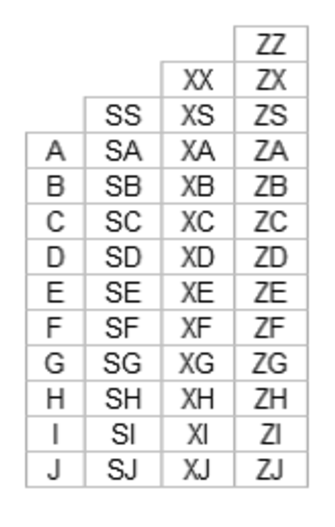
\includegraphics[width=5cm,clip]{res_x_i/tw0.eps}
 \end{center}
 \caption{レベル一覧}
 \label{x_i:tw_level}
\end{figure}

\answer{僕}{僕は SS だから……中間程度!? e-typing 1 ページ目常連のこの僕が!?}

\answer{精}{スペースを押すのにも慣れていない状態で初見常用 SS なら、それなりだと思いますよ。慣れたら X の半ばから X の上の方くらいまではすぐ行けると思います。}

\answer{僕}{XE とかってこと? それってレベル的にどうなの?}

\answer{精}{どこに出しても恥ずかしくないタイパーだと思います。ただ、上には上がいる世界なので……さっきの GANGAS のページからランキングを見てみるといいんじゃないでしょうか。}

\answer{僕}{Z ばっかりじゃん……どこだよ、どこだよ XE ……オウフ、一番下ですか……1000 位とか……。}

\answer{精}{今の記録と比べるなら、SS というと 50 秒以上かかってますから……トップレベルの人は倍以上速く打っていますね。}

\answer{僕}{レベル高すぎワロエナイ。}

\answer{精}{同じワードを何年も打ち込んだりしているわけですしね。打ち切り回数(最後まで打ってタイムを出した回数)も千とか万とかの世界です。e-typing のようなペラペラのランキングとは違うんですよ。10 年積もり積もった結果ですから。日々ランキングを励みにコツコツ記録を伸ばしていって、いつかは憧れの 50 位以内(一番上の枠)に……! と、こういうスタンスで見るものです。}

\answer{僕}{やる気はあるつもりだったけど、ちょっと気が遠くなるかも……。}

\answer{精}{まだまだ伸び盛りですし、心配は要りません。今の自分のレベルより一つ上を目指し、もう一つ上を目指し……とやっている間に、いつの間にか成長しているものです。}

\answer{僕}{ステージをひとつずつクリアしていくって感じなのね。}

\answer{精}{まさにそれです。ランキングに関して、ちょっとモチベーションになりそうなことも言いましょうか? 国内にはこれ以上ハイレベルなランキングは存在しないので、ここで 100 位になれば、かなり堂々と全国 100 位を自負できます。というか国内歴代 100 位ということなので、現役タイパーの中でなら間違いなく 100 位以内と言えるでしょう。}

\answer{僕}{それは嬉しいな。}

\answer{精}{ちなみに、各ソフトのランキングは「総合ポイント」という得点のようなもので競われています。}

\answer{僕}{何がポイントになるわけ?}

\answer{精}{4 つある各モードの自己最高記録のタイムです。まず各モードごとに、タイムに応じたポイントが計算されて、その総和がそのソフトの「総合ポイント」です。}

\answer{僕}{最高記録以外はポイントにはならないのか。}

\answer{精}{ちょっと極端ですよね。でも、だからこそ自己最高記録をどんどん伸ばそうと必死になるわけです。}

\answer{僕}{みんな、こんなに頻繁に自己最高記録を更新してるってこと?}

\answer{精}{そうです。現役競技者のハングリーさはものすごいですよ。ぜひ影響を受けて、少しずつでも記録を伸ばせるようがんばってみてください。}

\answer{僕}{まだわからない部分が多いけど……とりあえず打ってみて、ランキングに参加していればいいんだね。}

\answer{精}{まずはカンペキでしょう。……ランキングについては、本当はもっと色々紹介したいですが……自分で見て回って色々感じて欲しいので、この辺にしておきますね。}

\begin{screen}
なおランキングの参加方法ですが、各タイプウェルの中から記録がコピーできるので、それをメールで送ると、毎週土曜日に反映されます。即時反映でない点も面白いところです。目立った更新だった場合はトップページで紹介されることも。

参加方法について詳しくは、GANGAS 公式の解説\footnotemark を熟読してください。
\end{screen}
\footnotetext{\url{http://members.jcom.home.ne.jp/gangas2/entry.html}}

\subsection{使い方}

全タイプウェルをせっせとインストールした僕。わざわざ全部インストールしたのを見届けた後に、あっけらかんと彼女はこう言う。

\answer{精}{タイプウェルは基本 4 種類あるという話をしましたけど、今からは国語Rに限定して話を進めます。}

\answer{僕}{OH!? タイプウェルオリジナルという謎のソフトに心惹かれてるんだけど?}

\answer{精}{タイプウェルの活用の仕方を身につけて欲しいと思うんですけど、国語、英単語、オリジナルそれぞれ仕様が違って面倒なんです。それに、英単語やオリジナルは e-typing や国語 R とはワードが全然違って、完全に別の競技です。今の段階で手を出すのは早すぎますね。英単語やオリジナルもオールラウンドに打てれば、それはすごいですけど……まずは国語Rに専念してタイプウェルという文化そのものに慣れるのをおすすめします。}

\answer{僕}{うー……了解しておくけどさ。}

\answer{精}{まあ、細かい点が違うだけなので、まず国語Rをおさえておけば大丈夫です。応用が利きます。これがタイプウェル国語Rの基本画面ですね。}

\begin{figure}
 \begin{center}
   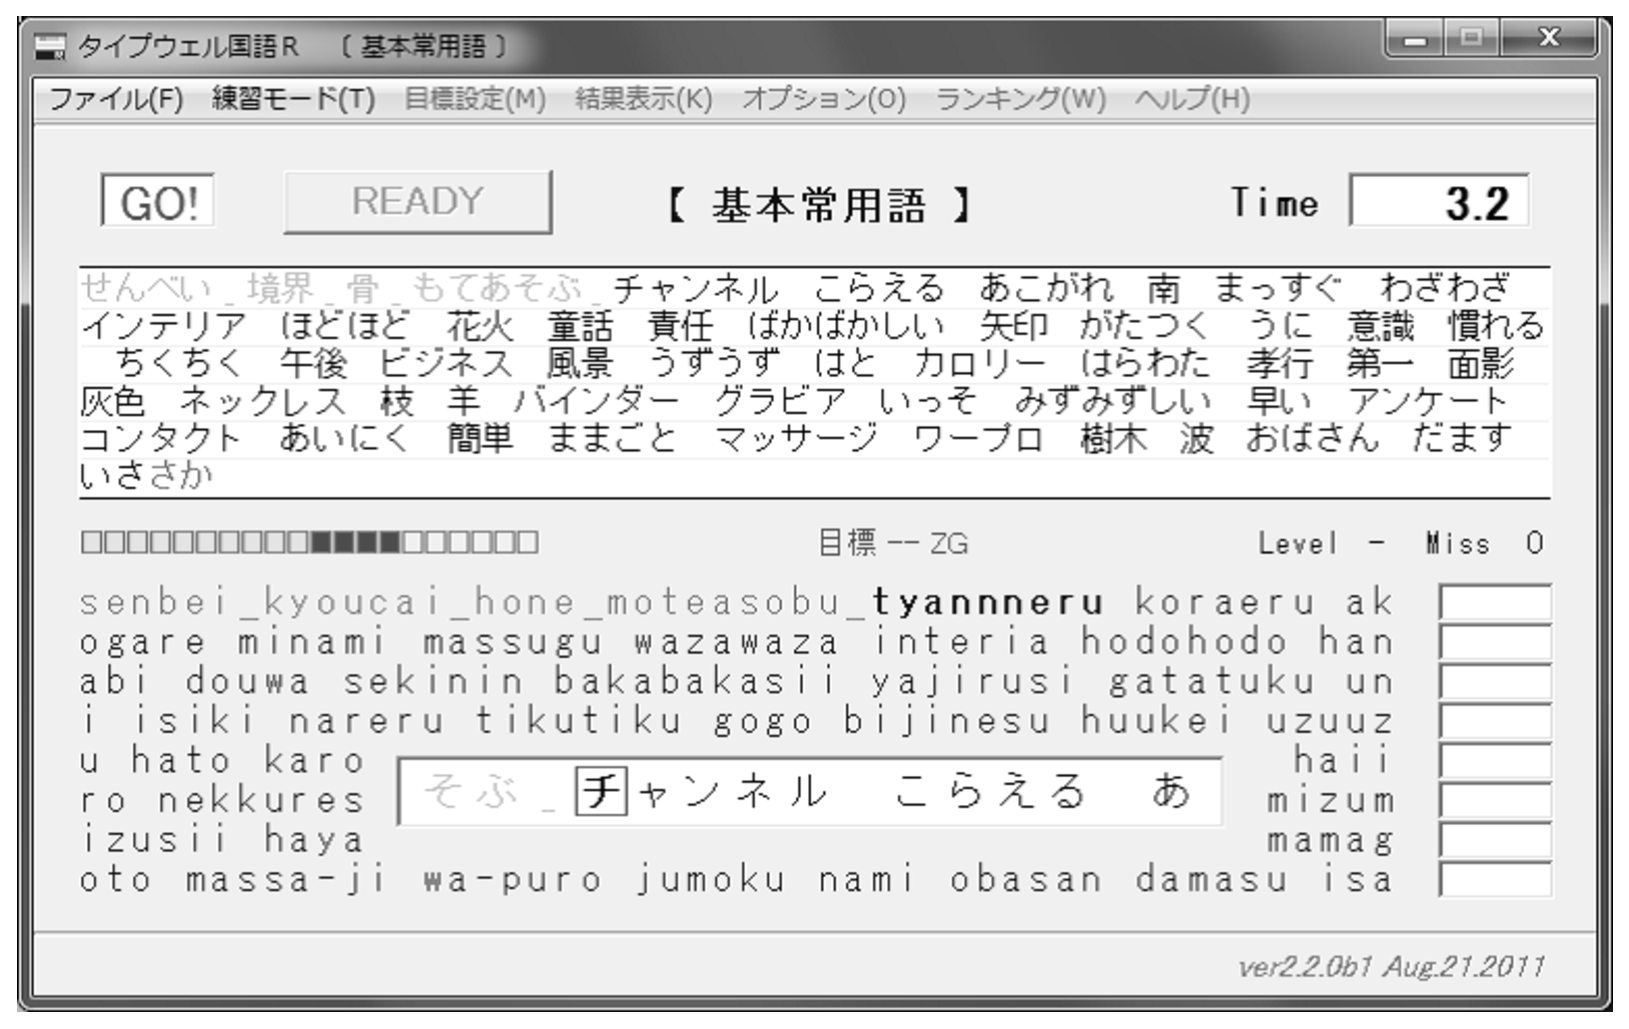
\includegraphics[width=7cm,clip]{res_x_i/tw1.eps}
 \end{center}
 \caption{タイプウェル国語R}
 \label{x_i:tw_mainwin}
\end{figure}

\answer{僕}{機能が詰まってる感じがするよね。}

\answer{精}{言い出せば本当に色々な機能があるんですが、全部解説して、活用法を書き出すとこれだけで本が一冊できちゃうので、タイプウェルプレイヤーなら絶対におさえておきたいポイントを見ていきましょう。}

\subsubsection{基本}

\answer{僕}{この READY っていうボタンをクリックでスタートして……とかそんなことはわかってるから。情強勢甘く見ないでね。}

\answer{精}{いえ、クリックする人は完全に情弱で、普通\key{Space}キーを使います。\key{Enter}でもいいですけど、手をホームポジションに自然に置いたまま、\key{Space}でスタートするのがベターでしょう。}

\answer{僕}{あーそっか。でも e-typing もスペースでスタートだったから、慣れてる。}

\answer{精}{\key{Esc} で中断できるのも e-typing と同じですね。これはある意味一番重要な機能かもです。}

\answer{僕}{……わお、本当に一瞬で中断できる。良い感じに打てるまで何度もこれでやり直せばいいと。}

\answer{精}{そういうスタンスもありますけど、はじめは毎回打ち切る(中断しないで最後まで打つ)ことをオススメします。タイプウェルの特徴のひとつに、記録が色んな面で蓄積されるという点があるんです。だからダメな記録でも、打ち切って蓄積すると……後から嬉しいかもしれません。}

\answer{僕}{他には?}

\answer{精}{先ほども説明しましたけど、各ワードの間に空白が挟まって出題されます。この空白部分では\key{Space}を毎回押さなきゃいけません。}

\answer{僕}{慣れないなぁ、これ……。}

\answer{精}{誰でも最初はそう思うんですけど、慣れてくると親指で\key{Space}を打つのはほぼ完全に無意識になります。なので最初ちょっとイラッとしても、そこは我慢です。我慢して慣れるだけの価値がタイプウェルにはあります、絶対。}

\answer{僕}{右親指で打つか、左親指で打つかは、どっちでもいいわけ?}

\answer{精}{さすが、良いところに気がつきますね。ですが、どちらで打つ人もいて、どちらが有利という結論なんてのは出ていないです。なので、どっちでも良い感じなのですが……ただ、後から変えるのはかなり大変なので、自分で納得した方で打つようにしてください。}

\answer{僕}{そんなこと言われても、余計困るよ。}

\answer{精}{うーん、完全に個人的な意見でよければ、左を薦めます。右手は\key{N}\key{M}周りでの最適化があったり、\key{-}\key{p}など遠目のキーが多かったりするので、左親指を使う方がわずかに有利なんじゃないかと。最適化をしない標準運指スタイルですと、また違ってくるんですけど。また、多くの人は右利きなので、右で打つ方がいいのではという意見もあります。結局、合う・合わないで決めるしかないでしょうね。}

\answer{僕}{うーん……。}

普段のタイピングでも左親指を使っていた僕は、少し悩んだあと、やはり左で打つことに決めた。こういうのは勢いだ。

\answer{精}{ゲームとしての操作方法は、これだけですね。シンプルです。}

\subsubsection{設定}

\answer{僕}{メニューバーに大量に項目があるけど……。}

\answer{精}{ほぼすべての機能がそこから呼び出せるようになっています。タイパーはキーボードが好きなので、慣れてくるとキーボードショートカットを使うはずですけど……慣れてないうちはメニューを開いて、見て回るといいですね。そこにショートカットキーも載っているので、見ているうちに覚えます。}

\answer{僕}{大体どういう機能があるのかも、見ればわかるね。}

\answer{精}{本当に重要な部分だけ見てみましょう。「練習モード」は 4 つあると説明したモードの切り替えですね。}

\answer{僕}{それぞれワードが違う、と。}

\answer{精}{記録もモード別にまったく別に集計されます。当たり前ですけど。「カタカナ語」「漢字」「慣用句・ことわざ」はそれぞれ難易度が高いので、慣れないうちは「基本常用語」一本でいいでしょう。文字通り、基本ですから。慣れてきたら総合成績を意識して、それぞれ攻略してみると面白いです。}

\answer{僕}{「目標設定」は?}

\answer{精}{目標を設定すると、プレイ画面にあるゲージ(インジケーター)で今の記録の目安をリアルタイムに確認できるんです。}

\answer{僕}{それはぜひ詳しく。}

\answer{精}{目標より速いペースか、遅いペースかが、インジケーターの表示になります。速いと青ランプが、遅いと黄・赤のランプが増えていきます。詳しい動作は、実際にプレイして確認した方がいいですね。}

\answer{僕}{まず、目標で高いレベルが設定できないんだけど……。}

\answer{精}{そこもポイントで、今出ている最高記録のレベルよりひとつ上までしか目標に設定できないんです。}

\answer{僕}{ああ、新しいレベルを出すと次のステージが解放されるんだね。レベルをひとつずつクリアしていくって、こういうわけか。}

\answer{精}{そうです。はじめはポンポンと自己最高記録が出せると思うので、まずはどこまで行けるかトライしてみるといいですね。ちなみにゲージの速度は「オプション」内の「目標インジケーター設定」で変更可能です。埋もれてますけど、これは大事な設定項目ですね。}

\answer{僕}{速く動くようにしておけばいいかな?}

\answer{精}{人によって好みがありますね。速く動きすぎると、そこに目が行ってしまって集中できないという人がいます。そういう人は遅くしたりしますし。}

\answer{僕}{他のオプションは弄らなくていいの?}

\answer{精}{インジケーターに比べると重要度は落ちます。お好みでどうぞ。}

\begin{screen}
「画面サイズ」は大きい方が文字が認識しやすくて良い、「カウントダウン設定」は「すぐにスタート」じゃないとイライラする、ミスの音はいらない、などなど、人によって色々な好み・こだわりはあります。
タイプウェルは本格的に取り組むと年単位でお世話になるので、プレイしているうちに勝手にそういうこだわりが出てきます。
\end{screen}

\subsubsection{結果表示}

\begin{figure*}
 \begin{center}
   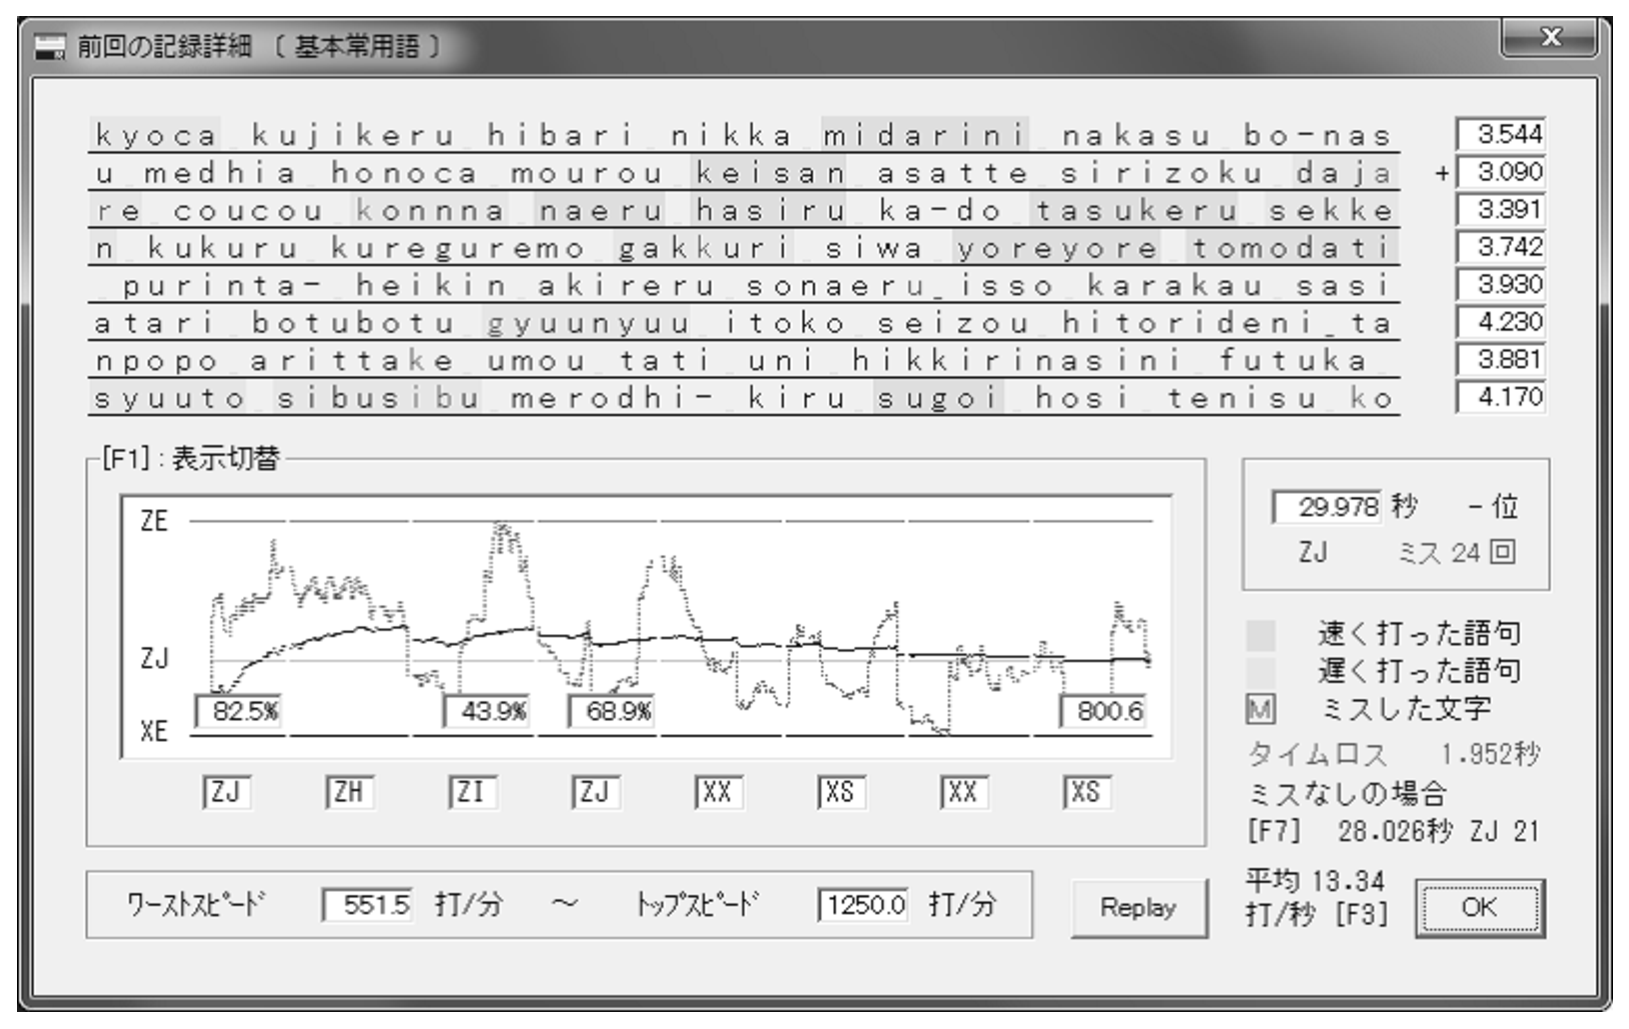
\includegraphics[width=14cm,clip]{res_x_i/tw2.eps}
 \end{center}
 \caption{記録詳細画面}
 \label{x_i:tw_record}
\end{figure*}

\answer{精}{最後まで打ち切ると、こういう画面が出ると思います。「記録詳細」画面ですね。}

\answer{僕}{似たのは出るけど……こんなグラフみたいなのは表示されてないよ。}

\answer{精}{その画面で \key{F1}を何度か押してみてください。押す度に表示が切り替わります。そのうちの一つの表示モードがこのグラフ表示ですね。一番情報量が多いので、玄人はこの表示モードで見ることが多いです。}

\answer{僕}{っていうか超速い記録じゃんこれ! Z とか出てる。}

\answer{精}{私がそれなりに真剣に打つとこんな感じですね。見方はわかります?}

\answer{僕}{わ、わかるよ。……と言いたいとこだけど、よくわからないのもある。}

\answer{精}{打ち切りタイムとか、この打ち切りのレベルとか、ミス回数とかは大丈夫でしょう。}

\answer{僕}{その上に並んでる数字は?}

\answer{精}{「ラップタイム」と呼ばれています。国語Rは400打鍵のタイムを競いますが、それを8のラップに分けて考えることがあります。}

\answer{僕}{各ラップ 50 打鍵……この画面のアルファベットの一行分がラップなんだね。ちょうど 8 行あるから。}

\answer{精}{そういうこと。こうやって分割することで、序盤で速かったけど後半が遅くなった、なんていう大体のプレイ結果を考えやすくしてあるんです。ちなみに各ラップのことを 1 ラップ目、2 ラップ目、なんて呼びますね。}

\answer{僕}{この例だと、3 秒で打っているラップもあれば、4 秒以上かかっているラップもあるね。}

\answer{精}{ラップごとにレベルも表示されていますね。グラフの下にレベルが並んでいるのがそれです。そしてこのグラフでは、もっと細かくスピードの推移を見ることができます。グラフ上の好きな位置にカーソルを合わせると、その地点が上の打鍵内容のどこにあたるのか、またその瞬間の速度はどれくらいだったのか、調べることができるんですよ。}

\answer{僕}{一番スピードが速かった瞬間は…… 3 ラップ目の中盤「萎える」「走る」のあたりか。本当に詳細だ。}

\answer{精}{一番速かったところの速度を「トップスピード」、遅かったところの速度を「ワーストスピード」と呼んでいます。下の方にそれぞれ分速何打のペースか、出てますよね。}

\answer{僕}{一番遅いところでも 551.5……僕の e-typing よりずっと速いってことか。}

\answer{精}{\key{Space}も打鍵にカウントしていますし、ワードごとの小休止なしでずっと続けて打ちますから、e-typing と単純に比較はできないですけど……大体のペースのイメージは湧きますよね。Weather Typing で一瞬だけ高速に打つ練習もしましたから、トップスピード 1250 打/分がどれくらい速いのかも想像がつくんじゃないでしょうか。}

\answer{僕}{「萎える」は\key{U}を中指でっていう最適化を使えば一瞬で打てそうだもんね。}

\answer{精}{e-typing でもやった先読みも駆使して、今打っているワードの次の単語・次の次の単語くらいまでは認識できてますから、組立が間に合えば最適化も使えますね。ワードの種類もそんなに多くない(各モード 2000 程度)ので、ワード慣れもできますし。}

\answer{僕}{今までやってきたことをすべて駆使して挑む……燃えざるを得ないシチュだよ、これは。}

\answer{精}{慣れれば慣れるほど面白いですよ。打つだけでどんどん伸びる時期はそれでいいですけど、伸び悩んできたらこの記録詳細画面で自分の打鍵をよくチェックして、改善点を探したりするといいです。}

\answer{僕}{他にも色々結果を見れる画面があるんだよね?}

\answer{精}{他はいくつもの結果を一覧したり、最高記録を並べたりする画面ですね。個々のプレイの詳細じゃなくて、統計的にどうなのかを見たい時に使います。ショートカットキーが \key{F5}\key{F6}\key{F7} と集中しているので、その辺ポチポチ押してみるといいです。}

\begin{screen}
具体的には、次のような画面です。

\begin{itemize}
 \item トップ15 (\key{F5}):そのモードの自己15位までの記録を一覧。トップスピードやワーストスピードのランキングも。
 \item カナ別成績:各カナごとにかかった平均時間を一覧。
 \item 総合成績(\key{F6}):各モードの最高成績を並べて見られるほか、オンラインランキングで競うことになる総合ポイントが参照できる。
 \item 練習実績(\key{F7}):日々の練習回数、その日の最高タイムなどが参照できる。
\end{itemize}
\end{screen}

\subsection{攻略法?}

単語の間にスペースを挟むのに苦労しながらも何度か打つと、XI が出て、続けて XH が出て……次々に上のランクを出すことができた。

\answer{僕}{XG 出たよ! エーックス! ジー!}

\answer{精}{おめでとうございます。私の予言通りですね。XD くらいまではこのまま行けちゃうと思いますよ。}

\answer{僕}{いつもみたいに、その先へ行くための攻略法も教えてよ。XD なんてすぐ行くから、XA とか ZJ とかのレベルを目指す方法をさ。}

\answer{精}{行き詰まってから言われないとわからないですよー。}

\answer{僕}{もったいぶらないでいいじゃん、もう隠すことなんてないでしょ。}

\answer{精}{それはないですけど……どちらかというと逆で、「これが攻略法だ」って自信満々に教えることができるようなことって、もうそんなにないんですよ。今まで教えて来たようなことをタイプウェルに応用していくだけなんですから。}

\answer{僕}{でも行き詰まったら教えてくれるんでしょ?}

\answer{精}{うーん、つまり、個人差があるのですよ。実際に行き詰まったあなたを見たら、私はきっと「ここが悪い」「ここを改善しよう」ってアドバイスできます。でも今の段階じゃ、あなたがどういうスタイルになって、どこで伸び悩むかなんて、全然わからないわけで。}

\answer{僕}{誰にでも言えるような「攻略法」はない?}

\answer{精}{「スムーズに詰まらず打ちましょう」「速く打てるワードを速く打ちましょう」みたいな中身のないことは言えますよ? でも、実際にどうやって進んでいくかは十人十色。最適化をする・しないの選択だけでもガラッと変わってきますし、もっと細かなタイピングのスタイルによっても話が変わります。あなたがこれから目指すのは、そういう世界です。ゲームとしてソフトを攻略するという部分も少しは残るでしょうけど……それよりも、自分自身を見つめ、分析して、工夫して、練習して、記録を伸ばしていく、その過程・取り組み方が重要になります。}

\answer{僕}{それは、「攻略法」っていうよりは……。}

\answer{精}{「練習法」とでも言ったほうがいいですね。最後はそういう勝負です。知っているだけですごく記録が伸びるテクニックとか裏技……そんなものはこの先、基本的にないです。}

その目はいつになく真剣で、まだ底に残っていた僕の甘えを、見事に射貫いて気化させる。この先の世界こそ、彼女が見ている世界。彼女に追いつき、追い越すために挑まなければいけない世界なのだ。

\answer{僕}{……わかったよ。じゃ、行き詰まったら、アドバイスを頼むね。}

\answer{精}{自分でも考えてくださいよ? 私だって何でもアドバイスできるわけじゃないですから。自分のことは自分が一番よくわかると言いますし、最終的には、すべて自分でわかって、考えることができなきゃダメです。}

その時、僕は一人前になるのだろう。彼女という存在を、越えることができるのだろう。

そしてその時、彼女という存在は、\\
彼女の存在意義は――。

そこまでで、僕は考えることをやめた。左親指でスペースキーを打つ。カウントダウンが始まる。今はまだ、これが僕の見るべき世界だ。

\begin{screen}
攻略法は、いずれ練習論というべきものになっていくよ、と丸投げしてしまいました。入門記事であるこの記事の扱うレベルはここまで、ということです。
これより高度な議論が知りたければ、本物のトップレベルタイパーであるテル氏の執筆された次の記事「タイピング練習論」がそれです。高度な内容を含みますが、ここまでついて来て、実際に競技タイピングの世界に入ることができた方なら、きっと読み解いて、糧にできるはずです。
\end{screen}

\section{文化と天空}
\begin{screen}
冗談じゃねぇ! こんな所! 俺は一人で帰らせてもらうからな!\\
――俺◆gt4Uu5qyB2, 史上初のタイプウェル国語 R 総合 ZG を達成し
\end{screen}

\subsection{環境・目標・交流}
季節は移ろい、制服が衣替えになって久しい。エコという名目でクーラーもつかない学校のパソコン室では、窓という窓が開け放たれ、グラウンドから大会をひかえ力の入っている野球部の快音が響いてくる。

あれから僕は、パソコン部の中に、特にタイピングを専門の活動とするグループを作った。「毎日パソコン入力コンクール」という、僕らが表向き目標にできる大会もあったので、顧問に認めてもらうことは簡単だった。

現在のメンバーは僕を入れて四人。他のメンバーが年上で異性ばかりという環境にもそろそろ慣れて、日々タイピング練習に励んでいる。実力はというと、正直なところ僕以外の皆はまだまだだったが、僕のスピードを目標にしているらしい。成長速度はかなりのもので、ライバルとなれる日も遠くなく思えた。

\begin{screen}
高校生以下の方には「毎日パソコン入力コンクール」への出場を強くおすすめしたいです。\\
\url{http://www.maipaso.net/}

現実社会では大会のようなものが少なく、一般人の評価が得にくい競技タイピングですが、この大会だけは例外です。予選を通過すれば全国大会に出ることができ、さらにそこでも活躍すれば賞品がもらえるほか、立派な表彰も行われます。
甲子園出場並……というとさすがに大げさですが、「全国大会」など響きはすごいので、取り組んで結果を出すことができれば現実生活で大変評価されること間違いなし。昔は一般(専門・大学生・社会人)にも全国大会があったのですが、今では高校生以下しか全国大会への出場権がありませんので、ぜひ中高生のうちに、チャレンジしてみて欲しいと思います。
同年代の人達だけとの勝負なので、この記事で紹介してきたような、究極的で半端じゃなく速い全日本レベルの人でなくても入賞が狙え、現実的でいい目標だと思います。
\end{screen}

僕がこんな行動を起こしたきっかけは、もちろん某ヨウセイサンのささやきがあったからだ。

\answer{精}{ライバルがいると伸びますよ。}

\answer{僕}{少年漫画の基本だねー。適当に GANGAS で探そ。}

\answer{精}{それもいいんですけど、直接会えたり、話せたりする人がいると理想ですね。}

\begin{screen}
とは言うものの、やはりリアルで仲間を作るというのは難しいことも多いでしょう。

最近ですと Twitter 等の SNS でタイパー間の交流が行われているのが目立ちますので、そこに参加するというのを次点でオススメしておきます。「タイプウェル」とか「e-typing」等と検索すればザクザクとタイパーが発見できるでしょう。また本書のあとがきの著者紹介にも、著者勢の Twitter アカウントが載っています。興味がある方は、お気軽にフォロー・リプライしてください。
\end{screen}

……と、思い返していたところに、声をかけられる。

\answer{男}{ねえねえ、今タイプウェルレベル何だっけ?}

\answer{僕}{国語Rは今総合XBになったとこ。今月中には Machine 達成(総合 XA 到達)したいんだよね。}

\answer{男}{成長速ぇーな。全然追いつける気がしないわ。}

\answer{僕}{うーん、けっこう必死だから。……目標設定・自己分析はしてる? 「ひとつ上のレベルを目指すのはもちろんですけど、中期的な目標を立てたりとか、今の自分に足りないのは何かと考えたりとか、そういう意識も大事ですよ」とかなんとか。}

\answer{男}{なるほど……意識からして違うってか。俺はとりあえず Genius 乗せないと始まらないな。ちなみに Machine 乗せた後のことも考えてるわけ?}

\answer{僕}{なんとなくだけど。タイプウェルだけで言っても、英語・オリジナルは全然打ったことないし。全部やるっていうのは大変だけど……やりがいはあると思う。}

\answer{男}{よくやるよなぁ。俺とか国語 R の 4 モードだけで死にそうだ。}

\answer{僕}{やっぱ行き詰まると、他のをやりたくなるじゃん。そういう意味で気分転換にもいいし……色々やると補い合って伸びる部分もあると思うし。何より楽しいよ。新しい種目を苦戦しつつ攻略してくのは。}

\answer{男}{ふーむ、俺は今のとこ、国語 R も行き詰まってはいないからな。}

\answer{僕}{うん、そういう時期はどんどんそれだけやって伸ばしていいでしょ。ただ……タイプウェルばっかりやってるとミスバカになっちゃいがちだから、そういうのは気をつけて。今はまだ、速度重視で伸ばしてもいいと思うけど。}

\answer{男}{ご忠告痛み入るよ。しかし、そんなことまでわかってやってるとか、本当ぱねぇな。}

\answer{僕}{それは……私の場合はちょっと、ずるなんで。}

\answer{男}{ずる?}

\answer{僕}{ううん、何でもない。気にしないで。}

彼に正直に話をしたところで、信じてもらえるはずもないし、証拠も見せられない。今の僕の実力・知識そのものが証拠のようなものだと自分では思うけど……客観的に信用させる証拠たりえないことはわかっていた。

電波女子扱いは、ちょっと困る。オタク趣味だって隠してるんだから。

\subsection{情報発信}

帰宅して、すっかりタイピングソフトで埋め尽くされたデスクトップ画面に向かう。そして意識すれば……。

\answer{精}{おかえりなさいですー。今日もタイピング日和!}

\answer{僕}{やあ。}

彼女が現れる。

\answer{僕}{日和っていうか、毎日やってるじゃん。タイピングに向かない日なんてあるの?}

\answer{精}{ありますよー、寒い日とか。冬になると正直つらいですね。手袋とか靴下とかを手に装着すると暖かくなりますが、打ちにくいですし。}

\answer{僕}{(靴下……?)部屋自体を暖めるしかないのかな。}

\answer{精}{「風呂上がり効果」といって、お湯に手を浸した後だとすごくよく指が動くっていうのが知られています。血行が良くなるからですね。冬でも体ごと暖まりますし……それを利用するのもいいです。}

\answer{僕}{なるほどね……しかし、いつも思うんだけど、どこからそんな知識を仕入れてきてるわけ?}

\answer{精}{もちろん、人づてですよ。先人の知恵と、現役タイパー達の情報交換の中ででしょうか。そうやって今日も明日も明後日も、攻略は積み重なって、続いていくんです。だからあなたも、自分で気づいたこと、思ったことがあったらぜひ積極的に情報発信して欲しいです。}

\answer{僕}{情報発信……ネットのブログとかで?}

\answer{精}{そうです。タイパーをやっている人って、引退後の方も数えれば相当いますけど、現役だけで数えると……そんなにはいないので。貴重なんですよ。あなたみたいなバチバチやってくれる人。}

\answer{僕}{まあ、めちゃくちゃ人が賑わってたら、僕のところに勧誘に来たりしてないよね。}

\answer{精}{立派に成長してくれて私、感激です。}

\answer{僕}{うん。僕こそ最初は何事かと思ったけど……こういう世界があるってわかって良かったと思ってる。}

\answer{精}{泣きそうです。……なので、ついでに気が向いたら、どういう媒体・どういう形式でもいいので、競技タイピングに関したことを形に残してくれると……さらに泣きそうになります。}

\answer{僕}{調子いいんだから……でも、そういえばちょうど今日も部活の人と話したりしてたんだよね。ああいう情報を発信していけばいいのかな。}

\answer{精}{そう、語り尽くされたような情報でもいいんです。同じ事考えてる人がいるなーって誰かが思えるだけで意味がありますしね。それに、自分の記録を積極的に公開していれば、あなたのことをライバル意識してくれる人も増えます。}

\answer{僕}{そうなれば自分のモチベーションにもつながるわけね。いいよ、了解した。}

……と、頭の中で発声する。最近は、彼女を相手にして部屋の中一人で奇声をあげることもなくなった。

彼女に問いを発する頻度が減っていく。何もかも、慣れていく。非現実は現実へと溶けて、\ruby{渾然}{こんぜん}一体となっていく。この頃にはもう、この先に待っていることが何なのか、僕は予感していた。

\subsection{そして高みへ}

まもなくして、タイプウェル国語 R が総合 XA ―― Machine になった。文字通りの「機械」認定。長いようで、振り返ってみるとそうでもなかった道のり。

ここまで行けば調子に乗れる、なんて以前は思っていたけど……実際は全く違った。自分が速くなればなるほど、より速い記録の偉大さがわかってくる。思い上がりや先入観が消えて、純粋に自分の記録・他人の記録を見つめる、競技者としての眼力が養われてくる。

時をおかず、国語 R の Machine よりも難度が高いと言われる e-typing 腕試し 600pt を達成。初速・正確性重視の打ち方も同時に鍛えてきていたおかげなのは、言うまでもない。

速くて正確なタイピング。一体僕は、どこまで来たんだろう? もう、尋ねても良い頃だと思った。しばらくぶりに、彼女に問いかける。

\answer{僕}{ねえ。僕はどこまで来たかな?}

キーボードの上にうっすらと現れた彼女は、じっとこっちを見て、こう答える。

\answer{精}{それは、あなたが一番わかっているはずです。}

\answer{僕}{そうだね。じゃあ次は、何をすればいいかな?}

彼女はきっとこう答える。

\answer{精}{それも、あなたが一番わかっているはずです。}

……その通りなのだ。予感が現実になっていく。それでも、踏み出さなければならない。僕を導いてくれた、彼女を越えていくために。

\answer{僕}{じゃあ次が最後だよ。}

\answer{精}{はい}

\answer{僕}{僕は、君が望んだ僕になれたかな?}

\answer{精}{……もちろんです。}

満足そうに、でも少しだけ名残惜しそうに笑って、彼女はその姿を消した。

いなくなったわけではない。今もここに。しばらくの間、僕は刻印のはがれかかったキーボードから、目を離せないでいた。

こうして、あるべき形に、僕たちは戻った。

\section*{終章}
\begin{screen}
一生を棒に降りし男ここに眠る。彼は無価値に生きたり。\\
――高村光太郎、墓碑銘
\end{screen}

ふと我に返る。

集中し過ぎたのだろうか。記録更新ペースでの最終ラップ――その最中に一瞬、意識が飛んだようだった。

にもかかわらず……画面には「新記録樹立!」の文字が映し出されている。

打ち始める前に、高校時代のことを思い出していたからだろうか。何だか、追体験をしたような感覚がある。

――そこで僕は、未熟な誰かにタイピングを教えるのだ。

閃きが落ちてくる。可能性に過ぎないと思う一方で、僕はその解釈を受け入れたい気持ちで満たされた。

\answer{僕}{「『私は、どこまで行くんでしょう?』」}

――楽しいと思える限り、どこまでも。



\clearpage
\articlepart{�^�C�s���O���K�_}{�e��(vuttar)}

\section{�C���g���_�N�V����}

\subsection{�͂��߂�}

�u�ǂ�����΃^�C�s���O�������Ȃ�̂��H�v

���Z�^�C�p�[�ɂƂ��Ă͍ł��g�߂Ő؎��ȁA��Ɍ��������Ă����Ȃ���΂Ȃ�Ȃ����ł��B�������c�O�Ȃ���u���ꂱ�ꂱ������ΐ�΂Ƀ^�C�s���O�������Ȃ�܂���I�v�Ƃ����A�ǂ�Ȑl�ɂ����Ă͂܂閲�̂悤�Ȏw�j�͍��͑��݂����A�o���オ��C�z������܂���B�e�l�ɂ�茻���_�ł̎��͂�Ō��X�^�C���A���߂�u�����v�̌`���قȂ�ȂǁA�l�X�Ȗ�肪����A���ǁu�Ƃɂ������K����v�ȂǂƔ��Γ����̂Ă��邱�Ƃ������悤�Ɏv���܂��B

�������A���Z�^�C�p�[�Ƃ��Ă͂��̖₢���瓦��邱�Ƃ͂ł��܂���B���������߂�u�����v�Ƃ͉��Ȃ̂��A���́u�����v��L�΂����߂ɂ͂ǂ�ȗ��K������΂����̂��A�^�C�p�[�e�l����ɍl���Ă����K�v������܂��B�Ƃ͌����Ă��A��l��l�̍l���ɂ͌��E������܂��B���͂�Ō��X�^�C���A���߂�u�����v�͂��ꂼ�����Ă��A�ϋɓI�Ɉӌ����������āA�l������������Ă������Ƃ��K�v���Ǝv���Ă��܂��B

���̋L���ł́A�����g��F����ɂƂ��ă^�C�s���O�̏�B���@�Ɋւ���ӌ������̏����ƂȂ�悤�A���i�����l���Ă��邱�ƁA���H���Ă��邱�Ƃ��܂Ƃ߂Ă����܂��B�܂��A��B���@������Ő������Ȃ��Ă͂Ȃ�Ȃ���肪�����‚����邽�߁A�����������l�X�Ȗ��ɂ��G��Ă����܂��B

\subsection{���ӓ_}

����u��l��l�̍l���ɂ͌��E������v�Ə����܂������A���̍ł���Ⴊ�^�C�s���O�X�^�C���̈Ⴂ�ł��B�g�p����z��A�œK���̗L���E���x�A�ϑ��^�w�x�[�X�E�W���^�w�x�[�X�A���m���h�E�ō����x�h�Ȃǂ̃X�^�C���̈Ⴂ�ɂ��A���ꂼ��̃^�C�s���O�͑傫���ς��܂��B���ɉ^�w�x�[�X�A�œK���̗L�����d��ȈႢ�ɂȂ�Ǝv���܂��B�X�^�C�����ς��Γ��R��B���@���ς���Ă��邽�߁A�^�C�s���O�S�ʂɒʗp����c�_�����悤�Ǝv���ƁA�����������Ⴂ�ɔz������K�v���o�Ă��܂��B

�Ƃ͂����A�����܂ōl���Ęb��i�߂Ă����̂͑�ςł����A�������������g�ɂ��̔\�͂�����܂���B�����ŁA����͊�{�I�Ɏ��̃^�C�s���O�X�^�C���i������p�^�[���ʂ̒S���w�œK���̕s�̗p�A�^�C�v�E�F���d���A���m���E���萫�d���A�W���I�ȉ^�w�x�[�X���X�j��O��Ƃ��Ęb��i�߂Ă������Ǝv���܂��B�‚܂���e�I�ɂ́u�����܂Ŏ��̏ꍇ�͂����ł���v�Ƃ������x�̂��̂ɂȂ��Ă��܂��킯�ł����A���̃^�C�s���O�X�^�C������r�I�I�[�\�h�b�N�X�Ȃ��Ƃ�����A���Ӑ[���ǂ�ł���������΁A���̗l�X�ȃ^�C�s���O�X�^�C���ɂ��\���K���ł���Ǝv���Ă��܂��B

\subsection{���̋L���̑Ώێ�}

���̋L���́A������x�^�C�s���O�ɏK�n���Ă������A�����̕ǂ������Ă��������ȑΏۂƂ��Ă��܂��B�^�C�s���O���n�߂��΂���̕���A�S���ǂɒ��ʂ��������ɐ������Ă���l�́A���܂�[���l�����A�Ƃɂ������ނ����ɗ��K���Ă����̂��ǂ��Ǝv���Ă��܂��B�܂��A�m�ł��鍪���◝�_�ł͂Ȃ��A�P�Ȃ�o���⊴�o�Ɋ�Â��Ęb��g�ݗ��ĂĂ����̂ŁA�F���񎩐g�̌o����l�@�Ɋ�Â��Ĕᔻ�I�ɓǂ�łق����Ƃ������R������܂��B�n�߂��΂���̕��Łu����ł����e���C�ɂȂ�I�v�Ƃ����ꍇ�A2�`5�͂͂Ƃ肠����������Ɠǂݗ����āA��̓I�ȗ��K���@�Ɍ��y���Ă���6, 7�͂����ǂ݂����������Ƃ������߂��܂��B

\subsubsection*{�K�n�̖ڈ�}
\begin{itemize}
 \item �P�L�[�Ō��͖��ӎ������Ă���
 \item �������܂Ƃ܂�ő����Ă�ǂ݂Ȃ����͂ł���
 \item ��ǂ݂�������x�ӎ��ł���
 \item �Ƃɂ����ł��Ă���Ίy�ɍX�V�ł���A�Ƃ����������߂���
 \item �‚܂�Ƃ���u�F���E�g���E������A���s���Ă�����x��ǂ݂Ȃ��s����v�Ƃ�������
 \item �ڈ��Ƃ��Ă� �^�C�v�E�F������R ��p XF ���炢����H
\end{itemize}

\subsection{�u�����v�Ƃ͉���}

�u�ǂ�����΃^�C�s���O�������Ȃ�̂��H�v�Ƃ����₢�́A�P�������̂悤�ł��āA�悭�悭�l���Ă݂�ƈӖ���������܂���B�^�C�s���O���u�����v�Ƃ͂ǂ��������Ƃ��A�Ƃ������ɓ������o�Ă��Ȃ�����ł��B�Ⴆ�΃^�C�v�E�F������R��{��p��̋L�^���L�т��Ƃ��āA����Łu�^�C�s���O�������Ȃ����v�ƌ�����̂��A�Ƃ��������ł��B�ǂꂩ��‚̃\�t�g�i�Ⴆ�΃^�C�v�E�F���j�ŗǂ��L�^���o���Ă��A���̃\�t�g�i�Ⴆ�� e-typing �A���p�\�AWeather Typing �c�c�j�œ������x���̋L�^���o����Ƃ͌���܂���B�‚܂�A�e�\�t�g�́u�����v�͎��Ĕ�Ȃ���̂Ȃ̂ł��B

�e�\�t�g�́u�����v�����ꂼ��قȂ�Ƃ���΁A��̉����ǂ��Ⴄ�̂��A�Ƃ������Ƃ����ɂȂ��Ă��܂��B���l�̍l���Ƃ��ẮA�o�蕶�̓��e��Ō����A�o��̎d���A��t���͕����̍��قȂǁA�e�\�t�g�̓����ɈႢ������A���̌��ʂƂ��āu�e�\�t�g���v������\�́v���傫������Ă��邱�Ƃ���肾�ƍl���Ă��܂��B�u�����v���������l�i�� �u�Ō����x�v�u kpm �v�u��/�b�v�j�͓����ł����Ă��A���ꂼ��̃\�t�g�œ������l�ɒB���邽�߂Ɋe�\�t�g���v������\�͂��Ⴆ�΁A���ꂼ��̐��l�͕ʕ��ƌ����邾�낤�A�Ƃ������Ƃł��B

�Ⴆ�΁u���񓯂����͂��o�肳���\�t�g�i���p�\�A�̗w�^�C�s���O����A�^�C�v�E�F�����@�Ȃǁj�v�ł́A�����̗ǂ��^�w��y�[�X�z�������O�ɓ��̒��őg�ݗ��ĂĂ����A���x�����K���Ē蒅�����A�w�̉^���\�͂��ő���Ɋ��p����A�Ƃ������\�͂��d�v�ɂȂ邩������܂���B�u���܂����P��E���͂̒����烉���_���ŏo�肳���\�t�g�i�^�C�v�E�F���Ae-typing �A���i�łȂǁj�v�ł́A���̎��X�ʼn^�w��y�[�X�z�����l���˂΂Ȃ炸�A�^���\�͂��͔]���ł̏����\�͂��d�v�ɂȂ邩������܂���B

�܂��A�o�蕶�����ɂ���Ă��u�����v�𓾂邽�߂ɕK�v�Ȕ\�͂͑傫���ς���Ă��܂��B����ł�v���閈�p�\�ł͎��v�́A400�ŌŒ�̃^�C�v�E�F��(����R, E)�ł͍ō�������������\�́A�Z���� e-typing �ł͌������܂��ꂽ�W���͂��d�v�ɂȂ邩������܂���B

���̂悤�Ȋe�\�t�g�̓����̈Ⴂ��S�čl�����āA�e�\�t�g���ǂ̂悤�Ȕ\�͂��ǂ̒��x�v�����邩������o���A�X�ɂǂ̂悤�Ȕ\�͂��ǂ̂悤�Ȕz���Ŏ����Ă��邱�Ƃ����z�ł��邩�̍��ӂɎ���΁A�e�\�t�g�̐��т𑍍����āu��ΓI�ȑ����v���������Ƃ��ł��邩������܂���B�����������ɂ́A���Z���̓����͂�����x���������Ƃ��Ă��i���ۂ͋��Z�������̂̕��͂��܂��i��ł��Ȃ��Ƃ͎v���܂����j�A���ꂼ��̓�����L�����^�C�s���O���Z���ǂ̂悤�Ȕ\�͂�K�v�Ƃ���̂����悭�������Ă��炸�A�c�O�Ȃ����ΓI�ȑ������v�����邱�Ƃ͕s�”\�ł��B�܂������ɁA���鋣�Z�̋L�^��L�΂��ɂ͂ǂ̂悤�ȗ��K������΂������Ƃ��A���������߂�u�����v�����߂邽�߂ɂ͂ǂ��������K������΂������A�Ƃ������₢�ɂ����S�ȓ����͏o�Ȃ��Ƃ������ƂɂȂ�܂��B

�������A���Z�������v������\�͂̈Ⴂ��S���l�������ɗ��K����Ƃ����X�^���X�́A���܂�D�܂������̂ł͂Ȃ��ł��傤�B�������ǂ������u�����v�𓾂����̂��A�ǂ������\�͂�v�����鋣�Z���d�v������̂��A�Ƃ����W�]�̓^�C�s���O��[���y���ނ��߂ɏd�v�Ȃ��̂��Ǝv���܂����A�������̋��Z�̋L�^����݂̂��l����ɂ��Ă��A���̋��Z���v������\�͂��ᖡ���邱�Ƃ́i�Ⴆ�C�}�C�`������Ȃ������Ƃ��Ă��j�����I�Ȑ����𐋂��邽�߂ɏd�v�Ȃ͂�������ł��B�܂��A�������������ɂ‚��Ă̗������[�܂�Ȃ��ƁA�L�^�̈Ӗ��𐳂��������邱�Ƃ��ł��܂���B���l�̋L�^�A����Ɏ����̋L�^�𑸏d���邽�߂ɂ��A�F�ōl���Ă����Ȃ���΂Ȃ�Ȃ���肾�Ǝv���Ă��܂��B

\subsection{�����I�ȑË��_}

�Ƃ������ƂŁA���̖��𑽏��Ȃ�Ƃ��������邽�߁A���Ȃ�́u�e���Z���v������\�͂���ʂ���v���߂̕��@�ƁA���̏�ō���̋L�����ǂ������u�����v�����ɂ����̂��������A����Ɋ�Â������K�_��W�J���悤�Ǝv���܂��B

�܂��A�u�e���Z���v������\�́v�̑O�i�K�́A�u���������^�C�s���O�Ƃ͂ǂ������\�͂̑g�ݍ��킹�Ő��藧���Ă���̂��v�Ƃ����₢�̍X�Ȃ�O�i�K�Ƃ��āA�u�^�C�s���O�Ƃ͂ǂ̂悤�ȉߒ��ōs����̂��v�Ƃ������Ƃ��l���܂��B�����I�ɂ́u���ꂱ�ꂱ�̊튯������������Ƃ��Ď�e���Ĕ]�����������ēd�C�M���������ŋؓ��������������Ďw�����������āc�c�v�̂悤�ɁA�����ɂ��߂��ߒ����g�ݍ��킳���ă^�C�s���O���i�s����킯�ł����A������G�c�Ɂu�F���v�u�g���v�u����v�̎O�‚ɕ��ނ��Ă��܂��܂��B���̎O�‚̉ߒ��ɕ��ނ���΁A���ꂼ��̉ߒ��łǂ̂悤�Ȕ\�͂��K�v�ɂȂ邩�A�Ƃ��������Ƃ�����������₷���Ȃ邾�낤�A�Ƃ������_�ł��B���̍l����2, 3�͂ŏڂ����������A4�͂ł͗l�X�ȋ��Z�ɂ��̍l����K�p���āA���Z�̓����𕪐͂��܂��B

�������ă^�C�s���O�\�͂�������x���Ή�������́A�S�Ă̋��Z�����ɒʗp����`�ŋc�_��i�߂�͎̂��ɂ͕s�”\�Ȃ̂ŁA�قڃ^�C�v�E�F���݂̂ɘb���i��܂��B�u�^�C�v�E�F�����ǂ̂悤�Ȕ\�͂�v�����邩�v���g���C�A�����̃t�F�[�Y���ɕ��́i5�́j���A�u�^�C�v�E�F�����v������w�����x�v�𑼂̋��Z�ƈꉞ��r�ł���悤���Ή�������ŁA�^�C�v�E�F���̗��K���@�����i���̋��Z�ւ̓K�p�͊F����ɍl���Ă��炤�j�i6�́j�Ƃ������Ƃł��B���ꂪ����̋L���̑Ë��_�Ƃ������A���̌��E�Ƃ������ƂɂȂ�܂��B�܂��A7�͂ł͂����������g�g�݂͒E���āA�ǂ̂悤�ȋ��Z�ɂ����ʂ���A�R���f�B�V�����̒����E�����I�ȗ��K�v��E�����̃r�W�����E���`�x�[�V�����̈ێ��A�Ƃ�������ʓI�Șb��ɂ‚��Č��܂��B

\section{�^�C�s���O�̎O�v�f}

\subsection{�^�C�s���O�𕪉�����}

�O�͂Ő��������ʂ�A�^�C�s���O�͐�������Ȃ��i�K�I�ȏ������琬�藧���Ă��܂��B�����̏������ׂ����������A���ꂼ��̏������Ɏ��Ԃ�Z�k���邽�߂̑΍���l���Ă����΁A�������I�ɏ�B�ł���ł��傤�B�������A�ׂ���������Ε�����قǕ��S�͏d���Ȃ�܂����A�ו��ɂ�����肷���đS�̂������Ȃ��Ȃ��Ă��܂��Ƃ������Ƃ��l�����܂��B�����ŁA�܂��͑�G�c��2�`5�’��x�̗v�f�ɕ������Ă݂�ƁA�K�x�ɍׂ��������܂Ŗڂ��s���悤�Ɏv���܂��B���̏ꍇ�́A3�‚̗v�f�ɕ������܂��B
\subsection{�^�C�s���O�̎O�v�f}

���̋L���ł́A�^�C�s���O�̒i�K�I�ȏ������A�傫���u�F���v�u�g���v�u����v�̎O�‚ɕ������čl���܂��B�u�F���v�͉�ʂɕ\�����ꂽ�ۑ蕶�����F���E�L�����邱�ƁB�u�g���v�͔F����������������Ƃɔ]���őŌ������g�ݗ��Ă邱�ƁB�u����v�͔]���őg�ݗ��Ă��Ō���������ƂɁA���ۂɎw�𓮂������Ƃł��B���̏͂ł́A���̎O�v�f�ɂ‚��Ă̐��������܂��B�܂��A�O�v�f�̑��݊֌W�ɂ‚��Ă�3�͈ȍ~�ōl���܂��B

\subsection{�F��}

��ʂɉf���o���ꂽ�f�����Ƃ炦�A�ۑ蕶����Ƃ��ĔF�����A�L�����鏈���̂��Ƃł��B�Ⴆ�΁u�n�̎��ɔO���v�Ƃ����ۑ蕶���񂪕\�����ꂽ���A�u�n�E�́E���E�ɁE�O�E���v�ƔF�����邩�A�u�n�́E���ɁE�O���v�ƔF�����邩�A�u�n�̎��ɔO���v�ƔF�����邩�ŁA�F�����x�͑傫���ς���Ă��܂��B��ǂ݁i���ɔF�������ۑ蕶����̑Ō����삪�I���O�ɁA��֐�ւƉۑ蕶����̔F����i�߂Ă������Ɓj�ƁA��ǂ݂����ۑ蕶�����Z���I�ɋL�����邱�Ƃ��u�F���v�͈̔͂ɓ���邱�ƂƂ��܂��B

\subsection{�g��}

�F�������ۑ蕶�����Ō���\footnote{�Ō���Ƃ͉ۑ蕶����Ƃ͈Ⴂ�A���ۂɉ�������L�[�̕��т̂��Ƃł��B�u�F�s�v�Ƃ����ۑ蕶����ɑ΂��A�Ō���́ukoukou�v�ucoucou�v�ukoucou�v�ȂǕ����ɕ������ꍇ������܂��B���ȓ��͂ł���ΑŌ���́u���������v�ƂȂ�܂��B}�ɕϊ����A���̑Ō���ɑΉ�����Ō������]���őg���Ă�i�C���[�W����j�����̂��Ƃł��B�p�^�[���ʂ̒S���w�œK�����s�Ȃ��Ă���l�̏ꍇ�A�g�p����w�̑I���Ȃǂ��g���͈̔͂ɓ���܂��B�Ō���ւ̕ϊ��͌y�����ꂪ���̂悤�Ɏv���܂����A�d�v�ȏ����ł��B

\subsection{����}

�]���őg���Ă��Ō���������ƂɁA���ۂɎw�𓮂��������̂��Ƃł��B�悭�悭�l����ƁA�g���Ɠ���̋��ڂ͔��ɞB���Ȃ̂ł����A���̋L���ł͂��܂�[���l���Ȃ����Ƃɂ��܂��B

\subsection{�~�X�ɂ‚���}

�^�C�v�~�X��̑ł�������C���i���p�\�Ȃǂ̎��p���͂ł͕K�v�ɂȂ�j�ɂ‚��Ă��A�ʏ�̑Ō��Ɠ��l�Ɂu�~�X�̔F���v�u�ł������E�C������̑g���v�u���ۂ̑ł������E�C������v�ƁA�^�C�s���O�̎O�v�f�ɕ����čl���邱�Ƃ��ł��܂��B�����A�~�X�̔F���E�ł������E�C���Ȃǂ́A�{���͕ʘg�ōl���Ȃ���΂Ȃ�Ȃ����̂悤�Ɏv���܂��̂ŁA����͐[���l���Ȃ����Ƃɂ��܂��B

\subsection{�����̏��ԁH}

���̍l�����̂��Ƃł́A�^�C�s���O�́u�F�����g��������v�Ƃ����ߒ����o�čs����A�ƂƂ炦�܂��B�������A�ʂɁu�F�����g�������쁨�F�����g�������쁨�F�����c�c�v�Ƃ������Ԃōs����A�Ƃ����킯�ł͂���܂���B�^�C�v�E�F������R ��{��p��Łu���炩���߁Q�܂��܂��Q���ڂ낰�Q�v�Ƃ����ۑ蕶���񂪂������ꍇ�A�u���炩���߁v��F�����A�uarakajime�v�ƕϊ����A�Ō������g���āA�L�[���������I���Ă��玟�́u�܂��܂��v��F�����A�umazumazu�v�ƕϊ����c�c�A�Ƃ����킯�ł͂Ȃ��̂ł��B���ۂɂ́A�uarakajime�v�̕����̓�������Ȃ���A�umazumazu�v�̕�����g���āA�����Ɂu���ڂ낰�Q�v�̕�����F������Ƃ������悤�ɁA���ꂼ��̓���͕��s���Ă��܂��B�O�v�f�͊�{�I�ɂ͕��s���Ȃ���A�l�X�Ɋ֌W�������܂��B���̊֌W�ɂ‚��Ď��̏͂ōl���܂��B

\section{�O�v�f�̑��݊֌W}

\subsection{�O�v�f�̑��݊֌W}

���ۂ̃^�C�s���O�̋ǖʂł́A�u�F���v�u�g���v�u����v�̎O�v�f�͓Ɨ��ɐi�s����킯�ł͂Ȃ��A���G�Ɋ֌W���Ă��܂��B�‚܂�A�u�F�����x��700kpm(�ɑ�������ʂ̕�����/��)�A�g�����x��600kpm�A���쑬�x��650kpm������A�^�C�s���O���x�͈�ԒႢ�g�����x�ɑ������������A600kpm�ƂȂ�v�Ƃ����悤�ȒP���Ȃ��̂ł͂���܂���B���鎞�͔F����������������A�܂����鎞�͓��삪������������c�c�Ƃ����悤�ɁA�Ō����x�̃l�b�N�ƂȂ镔���͎��Əꍇ�i�o�蕶����A�g�̂␸�_�̏�ԁA�v���C���Ă���\�t�g�̓����Ȃǁj�ɂ���ĕς��܂��B�^�C�p�[�͂悭�u�����_�ł͔F�����������������Ă���v�Ƃ��u�w�̓��쑬�x���l�b�N�ɂȂ��Ă����v�Ƃ��������Ƃ������܂����A����́u���ۂ̋ǖʂł͑����������镔���͗l�X�ɕς�邯��ǂ��A���ɔF�����x���傫��������������悤�ɂȂ��Ă����v�Ƃ������Ƃł���A�Ƃ����_�ɒ��ӂ��Ȃ��Ă͂Ȃ�܂���B

\subsection{�O�‚̃L�[���[�h}

�ł́A��̓I�ɂ͎O�v�f�͂ǂ̂悤�ȑ��݊֌W�ɂ���̂ł��傤���B������l����ۂ̃L�[���[�h�́A�u���s�v�u�x�~�v�u�����v���Ǝv���Ă��܂��B���s�Ƃ͎O�v�f�������i�s���Ă���ʏ�̏�ԁA�x�~�Ƃ͎O�v�f�̂ǂꂩ�������Ă��Ȃ���ԁA�u�����v�Ƃ͎O�v�f�̂ǂꂩ���������Ă����Ԃ̂��Ƃ������܂��B

\subsection{���s}

������x�܂ŏK�n�����^�C�p�[�ł���΁A�^�C�s���O�̑����̏�ʂł́u�F���v�u�g���v�u����v��S�ē����ɍs�Ȃ��Ă���i���s���Ă���j��ԂƂȂ�܂��B2�͂ŗ�ɋ������悤�ɁA�u���炩���߁Q�܂��܂��Q���ڂ낰�Q�v�Ƃ����ۑ蕶����̂����A�uarakajime�v�̕����̓�������Ȃ���A�umazumazu�v�̕�����g���āA�����Ɂu���ڂ낰�Q�v�̕�����F�����Ă����A�Ƃ������悤�ȏ�Ԃł��B���̂悤�ɎO�v�f���u���s�v���Ă����Ԃ��A�ʏ�̏�ԂƂ��ĂƂ炦�܂��B

\subsection{�x�~}

�������A���ۂ̃^�C�s���O�̋ǖʂɂ͎O�v�f�����s���Ă��Ȃ���Ԃ�����܂��B�O�v�f�̈ꕔ�������Ȃ��Ȃ邱�Ƃ��A�u�x�~�v�ƌĂԂ��Ƃɂ��܂��B���ꂼ��̃^�C�s���O�̋ǖʂłǂ̗v�f���x�~���āA�t�ɂǂ̗v�f�������Ă���̂��A�悭�l���邱�Ƃ��d�v�ł��B

�x�~�̗�Ƃ��ẮA�^�C�v�E�F���̍ŏ��ƍŌオ���ɕ�����₷���ł��B�^�C�v�E�F������R�̍ŏ��Łu�i�J�n�j���炩���߁Q�܂��܂��Q�v�Ƃ����ۑ蕶���񂪕\�����ꂽ�Ƃ��܂��B�^�C�p�[�͈�u�Łu���A��A���A���A�߁A�w���炩���߁x���ȁv�ƔF�����܂����A���̎��͂܂��g���E����͋x�~���Ă��܂��B���̂��Ƒg�����n�����A�Ō�ɓ��삪�n�����܂��B�܂��A�^�C�v�E�F������R�̍Ō�Łu�Q���ڂ낰�Q�����炤�i�I���j�v�Ƃ����ۑ蕶���񂪕\�����ꂽ�Ƃ��܂��B����܂ŎO�v�f�͑S�ĕ��s���Ă��܂����A�u�Q�����炤�v�܂œǂݏI������i�K�ŔF�����x�~���A���̂��Ƒg�����x�~���܂��B�I�����O�̈�u�́A���삾���������Ă����ԂƂȂ�܂��B

���ɂ��v�f���x�~�����͂�����ł��������܂��B�Ⴆ�Αg���E����Ɏ�Ԏ�肷���Đ�ǂ݂𒆒f�����ꍇ�i�F���̋x�~�j�A�~�X�����Ă��܂��~�X���e���m�F���Ă���ꍇ�i�g���Ɠ���̋x�~�j�A���S�ɑł����ꂽ�ۑ蕶���񂪕\������A��u�ŔF���Ƒg�����I�����ꍇ�i�F���Ƒg���̋x�~�j�Ȃǂ�����܂��B

\subsection{����}

�F�����g����������A��ɍō����œW�J�����킯�ł͂���܂���B�󋵎���ŁA�ǂꂩ�̗v�f�A�������͑S�Ă̗v�f���������������܂��B�����‚������̋�̗�������Ă������Ǝv���܂��B

\subsubsection*{�P���ɓ���p�^�[��}

�F���E�g���E����̑S�Ăɂ����āA��������̂�����p�^�[�������݂��܂��B����p�^�[���ɒ��ʂ���΁A���R���ꂼ��̏����͌������܂��B�������[�h�œ���������o�Ă���ƔF�����A�u�킴�킴�v�u�����v�Ƃ�������p�^�[�����o�Ă���Ɠ��삪�A�X�y���ł�����������l�͑ł������Ώۂ̕������o�Ă���Ƒg������������A�Ƃ�������ł��i�Ⴆ�� \key{C} �� \key{K} �̑ł����������Ă���l�́A�u���v���o�Ă���Ƒg�����������܂��j�B

\subsubsection*{���̗v�f�Ƃ̌��ˍ���}

���̗v�f�Ƃ̌��ˍ����ɂ���Ă��A���ꂼ��̏������x�͑傫���ς���Ă��܂��B�Ⴆ�΁u�Q�킴�킴�Q����ʂ�Q�v�Ƃ������ł��ɂ��������񂪌��������A���쑬�x���x���Ȃ�̂����z���ĔF������������ꍇ������܂��B�ł�����Ȃ������񂪏o�Ă��đg�����������A����ɔ����ē�����������A���̒x��𒲐����邽�߂ɔF������������A�ƘA�����Ă����ꍇ������܂��B�F���E�g���E����̂ǂꂩ�����������ŁA�قڏ�ɑ��̏��������������Ă���ꍇ���l�����܂��B

�^�C�s���O��B�̊�{�́A���́u�O�v�f�̌��ˍ����v���悭����߂邱�Ƃ��Ǝv���Ă��܂��B�Ⴆ�ΐ�ǂ݂����肸�l�܂��Ă��܂����ꍇ�A��ǂ݂���ʂ𑝂₷�i�F�������P����j���ƂőΉ����悤�A�Ƃ������ɍl����̂͑��v�ł��B���ꂪ�����u�������p�^�[���ɑΉ����邽�߂ɔF�����������A���̒���̔F���̗��Ē����i�F���̍ĉ����j���ł����ɋl�܂��Ă��܂����v�Ƃ����P�[�X�ł���΁A���P���ׂ��͂ނ��듮��\�́A�������͔F���̍ĉ����\�́A�Ƃ������ƂɂȂ�͂��ł��B�•ʂ̋ǖʂɂ‚��ď�ɂ��������l�@�����Ă������Ƃ͓���ł����A��{�I�ɁA�O�v�f����Ƀo�����X�ǂ��������Ă����A�Ƃ����ӎ������‚��Ƃ��d�v���Ǝv���܂��B

\subsubsection*{�ӎ��I�E���ӎ��I�ȃy�[�X����}

�F���E�g���E����̑S�Ăɗ]�T������A�‚܂�S�Ă̗v�f�𖳑ʂɌ��������Ă��܂��Ă���A�Ƃ����ꍇ���l�����܂��B����܂Łu�O�v�f�̑��x���֌W�������ă^�C�s���O���x�����߂Ă���v�Ƃ��������������Ă��܂������A���ꂼ��̔\�͂����E�܂ŋ�g���邱�Ƃ͓���̂ŁA���ۂɂ́A���K�ɂ���Đςݏd�˂��u���̂��炢�̃y�[�X�łȂ�łĂ�v�Ƃ����y�[�X���o�ɂ���āA��{�I�ȑ��x�𐧌䂵�Ă���͂��ł��B���̃y�[�X�����͈ӎ��I�ɍs���ꍇ�������ł����A���ӎ��I�ɍs���Ă���ꍇ������܂��B�u���̃y�[�X���z����ƑłĂȂ��v�Ǝv������ł��܂��A�{���̔\�͓I�ɂ͂����Ƒ��x���グ����͂��Ȃ̂ɁA���x��}���Ă��܂��ꍇ�ł��B��x�L�^��啝�X�V����Ɓu����A�łĂ邶���v�Ƃ��������ɂȂ��ē����x���̋L�^��A���ł�����A�����ԃ^�C�s���O����߂Ă��ċv���Ԃ�ɂ�蒼������啝�X�V�ł��Ă��܂����A�Ƃ����ꍇ�Ȃǂ́A��������z������Ⴞ�Ǝv���Ă��܂��B�啝�X�V�ň�i�K�����y�[�X���o����ɓ��ꂽ���Ƃ�A�����Ԃ̕��u�ɂ���ăy�[�X���o�����Z�b�g���ꂽ���Ƃɂ��A�{���̔\�͂��������ꂽ�̂ł͂Ȃ����A�Ƃ������߂ł��B

\subsubsection*{�R���f�B�V�����ƊO���I�v��}

�W���͂������Ă���ΔF���E�g���̔\�͂͒ቺ���܂����A�ؓ��ɔ�J�����܂��Ă�����A�����ɂ���Ďw����������ł���΁A����\�͂͒ቺ���܂��B�����������u�R���f�B�V�����v�͔��ɏd�v�ł��B�R���f�B�V�����̒����ɂ‚��Ă�7�͂ň����܂��B�܂��A�ۑ蕶�̕����T�C�Y��t�H���g�A�w�i�F�Ȃǂɂ���ĔF������������ȂǁA�O���I�Ȍ����v�����l�����܂��B�����������O���I�v�����^�C�s���O�̎ז������Ă��Ȃ����Ƃ������Ƃ��A���܂ɂ͍l���Ă݂�K�v������ł��傤�B

\subsection{�܂Ƃ�}

�F���E�g���E����̎O�v�f�́A�ʏ�̏�Ԃł͕��s���ē����Ă��܂��B�������A�^�C�s���O�̋ǖʂɂ���Ă͈ꕔ�̗v�f���x�~������A�������邱�Ƃ�����܂��B����v�f�̌����ɔ����đ��̗v�f���A���I�Ɍ���������A����v�f�̌��������z���Ĉӎ��I�ɑ��̗v�f��������������A�Ƃ������Ƃ�����܂��B�t�Ɍ����΁A����v�f�̔\�͂����P���邱�Ƃɂ���āA���̗v�f�ł̌�����h�����Ƃ��ł��܂��B�‚܂�A�F���E�g���E����̎O�v�f�̊�{�I�ȑ��݊֌W�́A�ǂꂩ�Ɏ�Ԏ��Α��̗v�f�ɂ����e�����y�ڂ��A�ǂꂩ�����P����Α��̗v�f�ɂ������̍D�e�����y�ڂ��A�Ƃ������̂��ƍl�����܂��B���������݊֌W�̋�̓I�Ȃ�����́A���ꂼ��̋��Z�̂��ꂼ��̋ǖʁA���̋��Z�ɑ΂���n�B�x�A�^�C�s���O�X�^�C���̈Ⴂ�Ȃǂɂ���đ傫���ς���Ă��܂��B�����������Ⴂ�ɂ‚��ẮA4�́A5�͂ōl���Ă����܂��B

\section{�O�v�f�̍l�����e�\�t�g�ɓK�p}

\subsection{�����Ƃ��}

���̏͂ł́A�O�v�f�̍l���������‚��̃\�t�g�ɓK�p���āA���ꂼ��̃\�t�g���e�ǖʂŔF���E�g���E������ǂ̂悤�ɗv�����邩���l���܂��B���̎��݂́A���ꂼ��̃\�t�g���v������\�͂𕪗ނ��āA����P��̃\�t�g�ł̋L�^�␬�ʂ𑼂̃\�t�g�̋L�^�␬�ʂƑΔ䂵�₷��������A���K�v��̌���ɖ𗧂Ă邽�߂̂��̂ł��B�������A�����̃\�t�g�͎����g�����܂��荞��ł��Ȃ����Ƃ�����A�l�@�̐��x�ɂ͂��Ȃ�^�₪�c��܂��B�O�v�f���g�������Z�����̕��ޖ@�̈����Љ���A�Ƃ������x�Ɏ󂯎���Ă���������Ώ�����܂��B�܂��A���̏͂�ǂ�Łu����A���̃\�t�g�̖{���͂���Ȃ��񂶂�Ȃ��I�v�Ǝv�����K�`���̕��ɔᔻ�E�ĕ��͂��Ă���������Δ��ɗL��ł��B

\subsection{e-typing �r�������x���`�F�b�N}

e-typing �ōł��l�C�̂���`���ł��B���6�`30�Ō��������x�̉ۑ蕶���\������A�����ł����݂܂��B�ۑ蕶�́A����I�ɕύX�����ۑ蕶�Z�b�g�̒�����A1�g���C�A���ɂ‚�15��o�肳��܂��B��‚̉ۑ蕶��ł��I����Ă��玟�̉ۑ蕶���\�������܂łɂ͏����Ԃ����邽�߁A1�����Ƃ̓Ɨ��������ɍ����A�����I�ɂ�15��̃g���C�A���̑g�ݍ��킹����Ȃ鋣�Z�Ɖ��߂��Ă����Ǝv���܂��B�ǂ̃\�t�g�ɂ������邱�Ƃł����A���̃\�t�g�ł͓��ɏK�n�x�i�����[�h����j�ɂ��v���\�͂̕ω����傫���̂Œ��ӂ��K�v�ł��B

�܂��Ae-typing ���n�߂��΂���`����Ȃ���x�ɂ������[�h���ꂵ�Ă��Ȃ��l�̏ꍇ���l���܂��B3�� 4�߁u�x�~�v�̕����ŐG��܂������A�ۑ蕶���o�肳�ꂽ����́A�F���E�g���݂̂��s���Ă��鎞�Ԃ����݂��܂��B�{�i�I�ɓ�����n�߂�ɂ́A���Ȃ��Ƃ�5�`6�Ō����͔F���E�g����i�߂�K�v�����邽�߁A���̉e���͖����ł��܂���B�X�ɂ��́u�ł��n�߂̕����v��15�񂠂邽�߁A���삪�x�~���Ă��鎞�ԁA�‚܂�F���E�g���݂̂�v�����鎞�Ԃ����̃\�t�g�Ɣ�ׂĔ��ɒ����A�ł��n�߂̔F���E�g���̑������L�^��傫�����E����ƍl�����܂��B�܂��A���l�Ɂu�ł��I���̕����v��15�񑶍݂��܂��B�ł��I���̕����ł͋t�ɓ���݂̂������i�F���E�g���͊��ɏI����Ă���j���ƂƂȂ邽�߁A����\�͂����E�܂Ŏg���ăX�p�[�g�������邱�ƂŁA���Ԃ�Z�k���邱�Ƃ��ł��܂��B�������ۑ蕶�̕����������Ȃ����߁A�ł��I���܂łɓ���̌��E���x�ɓ��B���邱�Ƃ͓���A���쑬�x��f�������߂�\�́i�����i�K�ł̓�������́j���d�v�ƂȂ��Ă��܂��B

���ɁAe-typing �̓���̉ۑ蕶�Z�b�g����荞�݁A�ɓx�Ƀ��[�h���ꂵ���l�̏ꍇ���l���܂��B�܂��F���́A�Ђ炪�Ȋ��Z�Ő�������ǂނ��A�S�̂������ƌ��邾���ŏI������i�ۑ蕶���o���Ă���̂ŁA�y���m�F����ΑS�����v���N������j�͂��ł��B�܂��A�g���ɂ‚��Ă͍X�Ɍ����ŁA�ۑ蕶�F���̌�A�������K�ɂ���Đςݏd�˂��Ō����o���ĂыN���������ŁA�g�����I������͂��ł��B�ۑ����Ă������Ō�������𓀂���A�ƃC���[�W����ƕ�����₷���Ǝv���܂��B���̂��߁A���[�h���ꂵ�Ă��Ȃ��l�� e-typing �ł͔F���E�g���̑��������ɏd�v�ɂȂ��Ă����̂ɑ΂��āA�ɓx�Ƀ��[�h���ꂵ���l�̏ꍇ�A�F���Ɋւ��Ă͊o�������[�h�𑦍��Ɉ����o�������A�g���Ɋւ��Ă͐ςݏd�˂��Ō����o�̐��x�Ƃ���������o�������A�������d�v�ɂȂ��Ă���ƍl�����܂��B�F���Ƒg���������ɍς񂾌�́A�Ђ�����ɓ���̑��x�Ɛ��x���v������邱�ƂɂȂ�܂��B�܂��A�ۑ蕶���Z�����Ƃ������̂ŁA�����ȓ���\�͂ɉ����A�����i�K�ł̓�������͂����ɏd�v�ƂȂ��Ă���Ǝv���܂��B���̂悤�ɁA�ɓx�Ƀ��[�h���ꂵ���l�̏ꍇ�Ae-typing �ŗv�������\�͂Ƃ��ẮA���|�I�ɓ���\�͂̔�d�������Ȃ�܂��B

���[�h���ꂵ�Ă��Ȃ��l�A���Ă���l�̏ꍇ�����ꂼ��l�@���܂������A���ۂ́u�S�����[�h���ꂵ�Ă��Ȃ��v�u�ɓx�Ƀ��[�h���ꂵ�Ă���v�Ƃ������Ƃ͒��X�����͂��ł��̂ŁA�ۑ蕶���Ƃ̃��[�h����̒��x�ɂ���āA��L��‚̊Ԃ��s�������邱�ƂɂȂ�Ǝv���܂��B��̓I�ɂ́A���[�h���ꂵ�Ă��Ȃ���΂��Ȃ��قǔF���E�g���̔\�͂��A���[�h���ꂵ�Ă���΂��Ă���قǓ���̔\�͂��d�v�ɂȂ��Ă���A�Ƃ������ƂɂȂ�ł��傤�B�܂��A�����i�K�ł̓�������͂́A���[�h����̒��x�Ɋւ�炸�d�v�ɂȂ��Ă���Ǝv���܂��i���邢�͂��ꂱ���� e-typing �̗v�_��������܂��񂪁A���ɂ͂܂��m���Ȃ��Ƃ͕�����܂���j�B

\subsection{Weather Typing}

Weather Typiing �i�ȉ� WT �j�̓����^���R���i�{���ł̃C���^�r���[�ɂ������Ă��������Ă��܂��B����������킹�Ă������������j������E���J����Ă���t���[�i�������J�j�̃^�C�s���O�\�t�g�ł��BWT �ł̓��[�h�Z�b�g�����삷�邱�Ƃ��ł��܂����A����̓f�t�H���g�̃��[�h�Z�b�g�i��̓I�ɂ� word1.txt �j�̎g�p��O��ɂ��܂��BWT �̃V�X�e���͓Ɠ��ŁA���[�h�Z�b�g�i�O���j�ƃ��[�h�Z�b�g�i�㔼�j��������Ă��āA���ꂼ��������_���ɑg�ݍ��킹�āA���ۂɏo�肳���ۑ蕶�����肳��܂��B�Ⴆ�΁u�����o���̒��Ɉ��̌����v�u�g�����J�[�e���R�[���v�ȂǁA���l�ȑg�ݍ��킹�̉ۑ蕶���o�肳��܂��B���̃Q�[���̏ꍇ�A���ߑł������i��ɒʐM�ΐ�B�ۑ蕶���m�F���悷���ɑłj�Ƃ��ߑł�����i��Ɉ�l�v���C�B�ۑ蕶���m�F������A�]���ŔO����ɑŌ������g�ݗ��ĂĂ���ō����őł������j�ő傫�����Z�������ω����܂��B

�܂����ߑł������̒ʐM�ΐ��z�肵�܂��B���̏ꍇ�́Ae-typing �ɔ��ɋ߂������������܂��BWT �ł́u�ۑ蕶�\������ł��n�߂܂ł̎��ԁv�̓J�E���g����Ȃ����߁A�F���E�g���̏d�v���͖{���Ⴂ�̂ł����A�ΐ�ŗI���ɂ���Ă���ƃ��[�h������Ă��܂����߁A�����I�ɂ͔F���E�g���̔\�͂��d�v�ƂȂ�܂��B�܂��Ae-typing �ɔ�ׂ�Ɖۑ蕶����r�I�������Ƃ������̂ŁA�����I�ȓ�������͂̏d�v���͎኱�Ⴍ�Ȃ�܂��B�������A��蕶�������Ȃ镪�A�����I�ȉ������I�����i�K�őł��I�����}������̂ŁA�ł��I���t�߁i�F���E�g�����x�~���Ă��镔���j�̑��x�ɓ���\�͂̍������傫���e�����܂��B

���ɂ��ߑł�����̈�l�v���C��z�肵�܂��B���̏ꍇ�A���ߑł������Ƃ͋��Z�Ƃ��Ă̓��������ɑ傫���قȂ�܂��B�܂��A�~�X�̊m�F��i�s�󋵂̊m�F�������΁A�F���\�͂��S���v������܂���B�ǂꂾ����������Ɩ�蕶��ǂ�ł��A���̎��Ԃ̓J�E���g����Ȃ�����ł��B�g���̑��x���������v������܂���B�������A�g���̐��x�i����𓮍�̐��x�ƌ����ɋ�ʂ���͓̂���̂ł����A����ɂ‚��Ă͖������܂��j�͗v������܂��B�Ō��������������g�ݗ��Ă��‚���ł��A���͍ו����B���ɂȂ��Ă��āA���̂����œ��삪�~�܂��Ă��܂��A�Ƃ����̂͂悭����b�ł��B�܂��A��������͂̉e�������ɏ��Ȃ��Ȃ�܂��B���ۂɑł��Ă݂�ƕ�����Ǝv���܂����A���O�ɑg����O����ɍs�����ƂŁA�ł��n�߂Ă����ɂقڍō����܂ʼn������邱�Ƃ��ł��܂��B�‚܂肽�ߑł������ WT �ɂ����ẮA�኱�̑g���̐��x�̑��́A�قƂ�Ǐ����ȓ��쑬�x�i����������́j�݂̂��v�������A�ƍl�����܂��B

\subsection{�^�C�v�E�F�����@}

�^�C�v�E�F�����@�̓^�C�v�E�F���V���[�Y�i GANGAS ��������E���J����Ă���^�C�s���O�\�t�g�B��͂�C���^�r���[�ɓ����Ă��������Ă���̂ŁA����������킹�Ă������������j�̈�‚ŁA�������́u�ʂ��v�ƁA�Z���`�����́u�����ʁv�̓�‚̃��[�h������܂��B���̓�‚̃��[�h�ɂ‚��āA�ʁX�ɍl���܂��B�b���ȒP�ɂ��邽�߁A�ʂ����[�h�ɂ‚��Ă̓��[�h����͂��܂肵�Ă��炸�A�����ʂɂ‚��Ă͂�����x���[�h���ꂵ�Ă���A�Ɖ��肵�܂��B�ʂ����[�h�͔��ɒ������ߑS���Ɋ���邱�Ƃ͓���A�����ʂɂ‚��Ă͒Z���Ԃɓ���������ł����ނ��ƂŊȒP�Ƀ��[�h����ł��邽�߁A�����ނ˖��̂Ȃ����肾�Ǝv���܂��B

\subsubsection*{�ʂ����[�h}

�ł��n�߂ɂ‚��ẮA���x���ł��Ă���Ίe�͂̎n�߂���\���������炢�܂ł͊o������̂ŁA�F���\�͂͂قڗv������܂���B���l�ɑł��n�߂̏\�������x�܂ł͎��O�ɑŌ������g�ݗ��ĂĂ����΂����̂ŁA�g���\�͂��قڗv������܂���B���������� WT �̂��ߑł��v���C�Ɠ��l�ɁA�ł��n�߂͂قړ��쑬�x�݂̂��v�������ƍl�����܂��B���̌�͈���I�ɎO�v�f�����s��������͂��ł����A�������A3�͂ŏq�ׂ��悤�ȗl�X�ȗv���ŕω����邱�Ƃ͂���܂��B���Ƀ^�C�v�E�F�����@�ł́A����̕��͂ł͖ڂɂ��Ȃ����̂⊿���̓ǂ݂��p�����邽�߁A�F���ʂŌ������₷���ł��B�܂��A�������ς�镔���ł́A��ǂ݂̂��߂Ɏ����𓮂����K�v������A�F���ʂł̑傫�ȕ��S����A�F���E�g���E����̑S�Ă���������܂��B���̑΍�Ƃ��ẮA���炩���ߑg���E�����x�点�ĔF���Ƃ̃M���b�v�����炷���Ƃ�A�ӎ��I�ɐ�ǂݕ��𑝂₵�ĔF���̗]�T����邱�Ɓi����͔��ɓ���悤�ȋC�����܂��B���͂���Ă��܂���j�Ȃǂ��������܂��B�܂��A�㔼�ɂȂ��Ă���ƏW���́E�؎��v�͓I�Ȗ�肪�o�Ă��܂��B�؎��v�̖͂��͓���ւ̈��͂ƍl�����A��ɖ��ʂ̂Ȃ��Ō����s������\�́i����̐������j��A��J�̒��x�ɉ����đł�����ς���悤�ȏ_��ȑg���\�͂����߂��܂��B�ł��I���̐������`�\�������͑��̋��Z�Ɠ����悤�ɓ��쑬�x�݂̂��v������܂����A�؎��v�͓I�Ȍ��E�����Ă���ł��낤���ƁA�S�̂̒��ł̊������ɒ[�ɏ��������Ƃ��l����ƁA���܂�d�v�ł͂Ȃ��ł��傤�B

\subsubsection*{�����ʃ��[�h}

�ł��n�߂ɂ‚��ẮA�ʂ����[�h�Ɠ������قړ��쑬�x�݂̂��v������܂��B�����ʂ̋L�^��_���ۂ͊�{�I�ɓ���������A�����đł‚��߁A�ۑ蕶�ɂ‚��Ă͂��Ȃ�̕����܂Ŋo���邱�Ƃ��ł��A�Ō���������o�Ƃ��ĕۂĂ邽�߁A��͂�قڑg���̐��x�E���쑬�x�݂̂��v������܂��B�������A������x���������̏ꍇ�́A�ۑ蕶���o���؂ꂸ�A�F���Ƒg���̔\�͂��v�������悤�ɂȂ�܂��B�܂��A�ō����ɋ߂���Ԃł�����x�����ԑŌ�����K�v���o�Ă��邽�߁A�؎��v�́E�W���͂Ƃ��ɑ����y�[�X�ŏ����܂��B�������ʓI�ɂ̓S�������ŏ��؂����x�Ƃ��v���܂��̂ŁA��J��Ԃɂ����Ă��F���E�g���E����̐��x�Ƒ��x������Ȃ����Ƃ��d�v�ɂȂ��Ă���̂�������܂���B

\subsection{�܂Ƃ�}

e-typing �AWT �A�^�C�v�E�F�����@�ɂ‚��āA���\�ʓI�ɂł͂���܂����A�O�v�f���ǂ̂悤�ɗv������邩���l�@���Ă݂܂����B���e�̑Ó����ɂ͋^�₪�c��܂����A�����������l�@��ʂ��Ă��ꂼ��̋��Z���ǂ̂悤�Ȕ\�͂�v�����邩���G�c�ɕ��͂��邱�Ƃ��ł���A�Ƃ������Ƃ͕������Ă���������Ǝv���܂��B���̕��͂̌��ʂƎ����̌��݂̔\�͂��Ƃ炵���킹�A�ǂ̔\�͂��ǂ����サ�Ă����Ό��ʓI�Ȃ̂��A�Ƃ������Ƃ��l���ė��K���Ă������Ƃ��d�v�ł��B

\section{�O�v�f�̍l�����^�C�v�E�F���ɓK�p}

\subsection{�����Ƃ��}

���̏͂ł́A�^�C�v�E�F������R ��{��p�� ���ɋ����A���Z�̊e�ǖʂłǂ̂悤�Ȕ\�͂��v������邩�ɂ‚��āA�O�v�f�̍l����p���āA�O�͂��͏������J�ɍl�@���܂��B���ꂼ��̋ǖʂŕK�v�Ƃ����\�͂𓥂܂��āA��̓I�ɂǂ̂悤�Ȃ��ƂɋC��t����ׂ����A�Ƃ��������Ƃɂ‚��Ă��G��Ă����܂��B����R ���̑��̃��[�h�ɂ‚��ẮA�Ō�ɊȒP�ɐG��܂��B

\subsection{�^�C�v�E�F���ŗL�̗v�f}

\subsubsection*{�X�y�[�X����}

�P��ƒP��̊Ԃ� \key{Space} �̓��͂�v���邱�Ƃ́A�^�C�v�E�F���̑傫�ȓ����ł��B������x���ꂳ������΁A\key{Space} ���͂̑��݂́A�F���E�g���E����̑S�ĂɍD�e�����y�ڂ����ƂƎv���܂��B�������A�{���ɏd�v�Ȃ̂́A���ꂼ��̗v�f�ɋy�ڂ��e���́g���x�h�ł��B\key{Space} ���ł��₷���ƌ����Ă�������x�̕��S�͂���͂��ł��̂ŁA���ꂼ��̗v�f�ɂǂ̒��x�̕��S�����邩�l���Ă݂܂��傤�B

���ۂ� \key{Space} �̉���������K�v������܂��̂ŁA����ɂ‚��Ă͊m���Ɉ��̕��S������܂��B�g���ɂ‚��Ă��A�����u\key{Space}�������v�Ƃ����Ō�����ł��A���ۂ̏󋵎���ʼn������͕ς�邽�߁A����Ō������g�ݗ��Ă�K�v������A�����̕��S�͂���͂��ł��B�������F���ɂ‚��ẮA\key{Space} �̑��݂͖��񕪂���؂��Ă��邱�ƂŁA���ꂼ��̒P�ꂾ���F������΍ςނ̂ŁA���̕��S�ɂ��Ȃ�܂���B����āA��{�I�� \key{Space} ���͂̑��݂́u�F���ʂ̕��S�����ΓI�Ɍy���Ȃ�v�Ƃ��������������炷�ƍl�����܂��B

\subsubsection*{�ۑ蕶����̎O�\�L}

�^�C�v�E�F������R�̉ۑ蕶����\�L�́A�ʏ�A��i�̊���������������\�L�E���i�̃��[�}���\�L�E���i�̗���镶���\�L ��3�‚ɕ�����Ă��܂��B�������ǂ��g�����ɂ���āA�F���ʂւ̕��S���ς���Ă��܂��B��Ɏ����ɍ�����������͍����邱�Ƃ��d�v�ł��B���ɔF���ʂ��l�b�N�ɂȂ��Ă���Ɗ����Ă���ꍇ�ɂ́A�܂����P���������ׂ��������Ǝv���܂��B

\subsubsection*{�P��P�ʂł̃����_���o��}

�^�C�v�E�F������R�̉ۑ蕶����o��`���́A�^�C�v�E�F�����@�̂悤�ȌŒ蒷���ł��Ae-typing �̂悤�ȕ��P�ʂł̃����_���o��ł��Ȃ��A�P��P�ʂł̃����_���o��ł��B\key{Space} �ɂ���؂�͂�����̂́A���4�`9�Ō����x�̒Z���P�ꂪ�Ԓf�Ȃ��o�肳��܂��B���̂��߁A�ɓx�Ƀ��[�h���ꂵ���Ƃ��Ă��A�Ō�����̉𓀁i4�� 2�߂��Q�Ɓj�͈�x��5�`10�Ō��������s�����A���x���J��Ԃ��s���K�v�����邽�߁A�g���̔\�͕͂ς�炸�v������邱�ƂɂȂ�܂��i���݂̎��̏ꍇ�A�Q�����������Ă��������𓀂Ƃ����悤�ȃ��x���ɂ��ǂ�‚��Ă��Ȃ��A�Ƃ��������ł����j�B����āA�P��P�ʂł̃����_���o��́A���[�h����ɂ��g���ւ̕��S�ቺ�����Ȃ��A�Ƃ��������������炷�ƍl�����܂��B�������A���[�h���ꂵ�Ă��Ȃ��i�K�ŁA�Ⴆ�� e-typing �Ƃǂ���̑g�����S�̊������傫�����A���Ƃ������͂܂��ʂ̘b�Ȃ̂ŁA���ӂ��K�v�ł��B

\subsection{�ł��n�߂̐�����}

�ł��n�߂̐������́A���̋��Z�Ɠ������A�F���E�g���̑f�����n�����d�v�ƂȂ�܂��B1�g���C�A���̑Ō�����400�����Ɣ�r�I���߂Ȃ̂ŁA�S�̂̒��ł̏d�v���͒�߂ł����A�΍�͕K�v�ł��B���̏ꍇ�A�ŏ��̐����������͗���镶���ł͂Ȃ����[�}����ǂ�Ŕ��˓I�ɑł‚悤�ɂ��邱�ƂŁA�F���E�g�����������Ă��Ȃ����ԁi����\�͂����ʂɂȂ��Ă��鎞�ԁj�����炷�A�Ƃ������j���Ƃ��Ă��܂��B�Ƃ͌������̕��j�́A���̌�ŁA���[�}�����痬��镶���ւ̎����̈ڍs�ƁA�Ō�����̑g�ݗ��ĕ��̕ύX�i�A���t�@�x�b�g�����Ĕ��˓I�ɑł‚�������A�Ō��`�����N��g��őł’ʏ�̂����ւ̕ύX�j���K�v�ɂȂ�A���̍ہA�F���ɂ�����x�̕��S��������܂��B���������������b�g�E�f�����b�g���l�����āA�����Ɍ��������j��T���̂��ǂ��Ǝv���܂��B

\subsection{1���b�v��}

1���b�v�ڂ̂����A�ł��n�߂̐��Ō��`�\���Ō����x�������������ł��B�܂��n�܂����΂���Ƃ������ƂŁA�F���E�g���E����Ƃ��Ɉ��肵�ɂ����A����ꂵ�₷���ǖʂł��B\key{Esc} �𑽗p����i1���b�v�ڂŎ��s�����璆�f����j�l�ł��A�Ⴆ��20���1�񂵂��܂Ƃ���1���b�v�ڂ�ł����Ȃ��Ȃ��̂ƁA10���1��͂܂Ƃ��ɑł����Ȃ���̂ł́A�����I�Ɍ���΋L�^�̏o���₷���ɑ傫�ȈႢ���o�Ă��邽�߁A1���b�v�ڂ͐�΂ɏd�v�ł��B

�F���E�g���E����𑁂��i�K����o�����X�ǂ��������邽�߂ɂ́A�܂��͑��x��������������̂�����Ǝv���܂��B���ɔF���i��ǂ݁j���\���������ł��̂ŁA�����ɋC���‚���K�v������܂��B��ǂ݂̗ʂ́A���߂͔�r�I���Ȃ߂ŁA�ォ�班�����‘������Ă����̂��ǂ����Ǝv���܂��B�܂��A�������ł��L�^��_�������A1���b�v�ڂ��狭���ɉ����������A�Ƃ����ꍇ�͂��̌���ł͂���܂���B

\subsection{2�`7���b�v�ڂ�8���b�v�ڑO��}

2�`7���b�v�ڂ�8���b�v�ڑO���ł́A��{�I�ɂ͔F���E�g���E����̑S�Ă����s����󋵂������܂��B���M���ׂ��_�́A���̕�����300�Ō��ȏ�̒���������A���̊ԗl�X�ɏ󋵂��ω����邽�߁A������x�Ջ@���ςɔF���E�g���E����̂������ς��Ă����K�v������Ƃ������Ƃł��B�Ⴆ�΁A�s���ς�钼�O�ɐ�ǂ݂̗ʂ𑝂₵�Ď����ړ��̔F�����S�ɔ����邱�Ƃ��ł��܂��B�t�ɁA�s���ς�钼�O�ɓ��쑬�x�������ĔF���̗]�T�����A�Ƃ�������ȕ��j���Ƃ邱�Ƃ��ł��܂��B�����I�ɑł��ɂ����P�ꂪ�������ɁA��ǂ݂��������炵�đg���̐��x����Ɉӎ��������A���J�ɑł����Ȃ����Ƃ��ł��܂��B�����u�M���M���X�V�y�[�X���A�����ŏ����ł�����������X�V�𓦂��I�v�Ƃ����󋵂ł���΁A�t�ɑg����a���ɂ��ĂƂɂ������o�ɔC���ăS�������A�Ƃ������j����������܂���B���Ȃ݂ɂ����̕��j�̌��莲�Ƃ��ẮA�F�����ǂ̒��x��s���邩�i��ǂ݂̗ʂƑ��x�j�E�g���̐��x�i���J�ɑł‚����o�őł‚��j�E���쑬�x �̎O�‚����l���Ă����΁A�Ƃ肠�����\���ł��傤�B

���̂悤�ɁA���݂̋ǖʂƂ��̃g���C�A���̑_���i�L�^�X�V�A���m������A���x����A���[�h����A���萫����c�c�j���l���ɓ���āA�Ջ@���ςɑł�����ς��邱�Ƃ��^�C�v�E�F���U���̌��ł��B�������A����Ȃ��Ƃ���������ƍl���Ȃ���ł‚��Ƃ͂ł��܂���B���i����g���C�A�����̑_������������ƌ��߂đł��A�ł��I������ۂɉ�������������΁A���v���C�����Ȃ���u���̋ǖʂł͂ǂ����ׂ����������v�Ƃ������Ƃ��ڂ���Ƃł������̂ōl���܂��傤�B������J��Ԃ����ƂŁA�������“I�m�ȏ󋵔��f��������悤�ɂȂ��Ă����Ǝv���܂��B

\subsection{�ł��I���}

�F���͑g���E����ɐ�s���Ă���i��ǂ݂��s�Ȃ��Ă���j���߁A�ł��I���̐������`�\�������ł͔F����Ƃ��s���K�v�͂Ȃ��A�g���E����ɏW�����邱�Ƃ��ł��܂��B���̂��߁A�����̏ꍇ�͂����郉�X�g�X�p�[�g�������邱�Ƃ��”\�ɂȂ�܂��B�����̓��쑬�x�̌��E�ɔ���‚���ŁA�S�Ă��o���؂�܂��傤�B���ɁA���X�g�X�p�[�g��������΍X�V�ł������ȏꍇ�Ȃǂ́A�ϋɓI�ɑ_���Ă����ׂ����Ǝv���܂��B�������A�X�V���ԋ߂ɔ������ŏI�s�͔��ɋْ����邽�߁A�t���Đn�̃��X�g�X�p�[�g�͑厸�s�ɂ‚Ȃ���₷���ł��B���i����ӎ��I�Ƀ��X�g�X�p�[�g���s�Ȃ��āA�����Ƃ������ɋْ����đ厸�s���邱�Ƃ̂Ȃ��悤�ɂ��܂��傤�B

\subsection{�ӎ��I/���ӎ��I�ȃy�[�X����}

3�� 5�߁u�����v�ł��G��܂������A���ۂ̑Ō��y�[�X�́A�F���E�g���E����̔\�͂����ł͂Ȃ��A�ӎ��I/���ӎ��I�ȃy�[�X�����Ɉˑ����Ă��܂��B���Ƀ^�C�v�E�F���ł͖ڕW�C���W�P�[�^��o�ߎ��ԕ\���Ȃǂɂ��y�[�X�c�������₷���A���̃y�[�X�ɕۂ��Ă��܂������ł��B�ӎ��I�ȃy�[�X�����͂����̂ł����A���ӎ��̃y�[�X�����͂��Ȃ���ŁA���΂��΋L�^����̖W���ɂȂ�܂��B����ɂ‚��Ă�6��4�߁u���ӎ��ɐݒ肵�Ă���V����O���v�ŐG��悤�Ǝv���܂��B

\subsection{���[�h���Ƃ̈Ⴂ}

�����܂ł͊�{��p���O���ɒu���ď����Ă��܂������A���̑��̃��[�h���d�v�ł��B�ȉ��ɏ�p�������3���[�h�̓����������Ă݂܂��B

\subsubsection*{�J�^�J�i��}

���{��ɂ͂��蓾�Ȃ������������p�^�[���̒P�ꂪ�����A�g���̕��S�������Ȃ肪���ł��B�܂��A���͂ނ��듮��͂��₷�����Ǝv���Ă��܂����A�^�w�̑����A�n�C�t������Ȃǂɂ��A����ɑ傫�ȕ��S��������l������悤�ł��B���Ȃ݂ɁA���w���g�p����W���^�w���̃^�C�p�[�̓J�^�J�i�𓾈ӂƂ���X��������悤�Ɋ����܂��B

\subsubsection*{����}

�Ƃɂ����u�ǂ݂ɂ����v�Ƃ����̂������ŁA�F���ւ̕��S�����ɍ����ł��B���̓��[�}���ǂ݂��̗p���Ă��܂����A���[�}���ǂ݂ɏn�B���Ă��A�����������Ɋo���Ă��A���炭�F���ւ̕��S�͈ˑR�Ƃ��č����Ǝv���܂��B

\subsubsection*{���p��E���Ƃ킴}

���[�h������������Z��������A�������܂܂�Ă����肵�āA�F���E�g���E����S�Ă��ɂ����Ǝv���܂��B�܂��A����R�ł͒���������̕��S���傫���i����\key{W} �������j���߁A����ւ̕��S���傫�߂ł��B

\section{�ǂ̂悤�ȗ��K�����邩}

�^�C�v�E�F���̋L�^�����シ�邽�߂ɂ́A��{�I�ɂ͗��K����݂̂ł��B�������A�ǂ̂悤�ȗ��K���A�ǂ̂悤�ɂ��ׂ����A�Ƃ����_�ł́A�F�X�ƍH�v�̗]�n������܂��B���̏͂ł́A�^�C�v�E�F���̋L�^�����߂邽�߂Ɂg�ǂ̂悤�ȁh���K�����ׂ����A�������͗��K�̓��e���ǂ̂悤�Ɍ��߂�ׂ����A�Ƃ��������Ƃɂ‚��āA���̌����������Ă����܂��B

\subsection{�{�g���l�b�N�����ɂ߂�}

�܂����ɁA�����̃^�C�s���O�ɂ‚��āA�{�g���l�b�N�i�ł��������������Ă���v�f�j�����ɂ߂邱�Ƃ��厖�ł��B����܂Ő������Ă����悤�ɁA���������������邩�͏󋵂ɂ���ėl�X�ɕς��܂����A����ł����ɑ������������Ă���v�f�������Ƃ���͂��ł��B��������ɂ߂邱�Ƃ͓���Ǝv���܂����A�K���������������‚����Ȃ������Ƃ��Ă��A�����ɂƂ��Ẳۑ��ϋɓI�ɒT���Ă����悤�ɂ���ׂ��ł��B���R�Ɓu�^�C�s���O�𑬂����悤�v�Ǝv���ė��K����̂ł͂Ȃ��A�u�����̔\�͂�L�΂����v�Ƌ�̓I�ȉۑ���C���[�W���ė��K���������������₷���A�������y�����Ǝv���܂��B

�{�g���l�b�N�����ɂ߂邽�߂ɂ́A�~�X�������茸�����Ă��܂������ɁA�u�ǂ����ċl�܂��Ă��܂����̂��v�����⎩�����Ă������Ƃ��K�v�ł��B�ȉ��̔F���E�g���E����̐߂ŁA���ꂼ��̗v�f�������ŋN���Ă��܂����s��A���P������@�ɂ‚��āA�����‚��̗�������Ă����܂��B

\subsection{�F���\�͂����߂�}

�F���ɗR�����鎸�s�ɕq���ɂȂ�ɂ́A�l�܂���\key{Esc} ��������ȂǂɁA��قǂ܂ł̎������u������ł��Ă���̂��v�u���ɉ���łĂ΂����̂��v�������ƕ������Ă������ǂ����A���₵�Ă݂Ă��������B�F�������Ȃ��s���Ă���΂ǂ�������R�Ɣc���ł��Ă���͂��ł����A���ۂ́A�茳�̑Ō��Ɉӎ���������������A��ǂ݂���s���������肵�āA�ǂ��炩���a���ɂȂ��Ă��邱�Ƃ������ł��B

�^�C�v�E�F���ɂ����ĔF���\�͂����߂�Ƃ������Ƃ́A��Ɂu��ǂ݂�K�x�ɁA�����m�ɍs����悤�ɂ���v�Ƃ������Ƃł��B��ɐ�ǂ݂Ɏ኱�̈ӎ��������A���ł��Ă�����e����������ێ�����K�v������܂��B���̂��߂ɂ́A��ɂ�����x�W�����āA�K�x�ȗʂ̐�ǂ݂�ێ�����悤�S�����đł‚悤�ɂ��Ă��������B�u��ɐS������v�Ƃ����͓̂�����ƂŁA���������a���ɂ��Ă��܂��A���̓x�ɋC��������ꊷ����H�ڂɂȂ�܂��B����ł���������ǂ݂͏�B���Ă��܂��̂ŁA�n���ɂ��ΐL�т���̂Ȃ̂��Ǝv���܂��B

\subsection{�g���\�͂����߂�}

����܂őg���Ƃ����v�f�̑��݂��A������O�̂悤�Ɉ����Ă��܂����B���������ۂ͂��̗v�f�͂Ȃ��Ȃ��ӎ�����ɂ����A���܂�d�v�����Ă��Ȃ��l�������悤�Ɋ����܂��B�Ō�����͂قږ��ӎ��ɍs���Ă��āA�g���R�X�g�͓���R�X�g�ɔ�ׂ�Ζ����ł���قǏ������A�Ƃ����l�����Ǝv���܂��B

�������A���͑S�������͎v���܂���B���̉^�w�͂�����W���^�w�ŁA�X�y���ł������ȊO�̍œK���͍s���Ă��܂���̂ŁA�Ō�����͔�r�I���ӎ��ɋ߂��͂��ł��B����ł����ۂ͖��ӎ��Ƃ͒������A�������́A������ӎ��I�ɐ��䂷�邱�Ɓi�g���̐������j�ɂ��Ō����x��啝�Ɍ���ł���A�Ɗ����Ă��܂��B�g���̉��P�ɂ���đŌ����x������ł����������‚������Ă݂悤�Ǝv���܂��B

\subsubsection*{�Ō��`�����N�̉��P}

����͑g���̉��P�̒��ł͍ł�������₷�����̂��Ǝv���܂��B�Ō��`�����N�Ƃ́A�����L�[�̑Ō�����‚̂܂Ƃ܂�������Ƃ��ĔF������ꍇ�́A��܂Ƃ܂�̂��Ƃł��i���̑���Ȃ̂ŁA��ʓI�ȗp��ł͂���܂���j�B����̑g�ݕ������P���邱�Ƃɂ��A�Ō����x�␳�m��������ł��܂��B

�������� �Ƃ����P����ɋ����܂��B\key{S}\key{A}\key{K}\key{U}\key{S}\key{A}\key{K}\key{U}��\finger{21872187}�őł‚Ƃ��܂��B����͌��X���ɑł��₷���A\key{S}\key{A}\key{K}\key{U}��1�‚̃`�����N�łƂ炦�A���R�ɑf�������͂ł��܂��B�������܂��܂����P�̗]�n�͂���܂��B������x�g���Ɠ���ɗ]�T������΁A\key{S}\key{A}\key{K}\key{U}\key{S}\key{A}\key{K}\key{U}��S��1�‚̑Ō��`�����N�ƂƂ炦�A8�Ō��ň�‚̓���Ƃ������o�őf�����ł������܂��B���̓���͂�������Ƒg�ݗ��ĂĂ����Ȃ��Ƃ����ɋl�܂�܂����A������x�L�p�ł��B�g���\�͂����܂�΁A���̂悤�ɑg���̕��S�𑝂₵���쑬�x�����シ����j���Ƃ邱�Ƃ��”\�ɂȂ�A�I���̕����L����܂��B

\subsubsection*{�ł������E�œK��}

�g���̕��S�����߂ē���̕��S��������A��ʓI�ŗL�p�ȕ��@�ł��B���͍œK���͍s���Ă��炸�A�ł��������܂����n�Ȃ̂ŁA�����œ��Ɍ�邱�Ƃ͂��܂���B

\subsubsection*{����̋󔒒n�т��Ȃ���}

�悭�悭�C��t���Ă݂�ƁA�w�̓����Ƃ��Ă͂܂��܂��]�T������̂ɓ����a���ɂ��Ă��܂��Ă��镔������R����͂��ł��B�Ⴆ��\key{Space} �̑O��A�ł��ɂ����P��Ō����������ƁA�Ō��`�����N�ƑŌ��`�����N�̊ԁA�Ȃǂ͂����Ȃ�₷���ł��B�W�����Đ�̕��܂ł�������Ƒg�������Ă���΃m�[�^�C���őłĂ镔���ł��A���R�ƑłĂΒx���Ȃ�A����\�͂𐶂�������Ȃ��Ȃ��Ă��܂��܂��B�F���̐�s�i��ǂ݁j���d�v�Ȃ悤�ɁA�g���̐�s���d�v�ł��B���R�Ǝw�������ɔC�����A��ɒZ�k�ł���ӏ���T���Ȃ���ł��i�݂܂��傤�B

\subsubsection*{��Ԕc���\�͂̌���}

������g���\�͂̂����̏d�v�ȗv�f�ł��B�Ⴆ��\key{U}�i\finger{7}�j��\key{N}�i\finger{7}�j�̂悤�ȃz�[���|�W�V�����O����z�[���|�W�V�����O�ւ̓��w�ٌ��ȂǁA��Ԃ���������c�����ē����g�ݗ��ĂȂ��ƃ~�X�ɂ‚Ȃ���₷���Ō��p�^�[���́A�����‚�����܂��B���m�ȋ�Ԕc�����ł��邾����ɋC��t����悤�ɂ��܂��傤�i���ۂ̂Ƃ���A��ԂƂ������͎w�Ƃ̑��ΓI�Ȉʒu�֌W�ɗ����Ă���C�����܂����j�B

\subsubsection*{�Ǐ����x�E�Ǐ����m���̃R���g���[��}

�Ō��p�^�[���̑ł��₷���A�󋵁A�g���C�A���̑_���A�]�T�Ȃǂ��l�����āA�Ǐ��I�ɑ��x�␳�m�����㉺������ꍇ������܂��B�X�V�_���̍ŏI���b�v�ŗ��ł����ă^�C�����҂��悤�ȁA���̂������̒�������Ƀ`�}�`�}���Ƃ������Ƃł��B����������ӎ����͂��߂��͍̂ŋ߂Ȃ̂ŁA���ɂ܂������邱�Ƃ��Ȃ��̂ł����A������x�]�T���o�Ă�����A�������������׍H���L�p�ɂȂ��Ă��邩�Ǝv���܂��B

\subsection{����\�͂����߂�}

�^�C�s���O�̗v�́A��͂蓮��\�͂ł��B��������߂邽�߂ɍł��d�v�Ȃ̂́A�w�̊�p�����̂����߂邱�Ƃł��B����������ɂ‚��Ă͗L���ȗ��K�@���������Ă��܂���B����͂Ƃ肠�����A�Ō��p�^�[���ʂɓ���\�͂����߂Ă����A�Ƃ������Ƃ��l���܂��B

\subsubsection*{���ȑŌ��p�^�[�����ӎ�����}

���v���C�̌������A�l�܂����P��̔������K�Ȃǂ�ʂ��āA���ȑŌ��p�^�[���𓪂ɐ��ݍ��܂��܂��傤�B�P���ɂ��̑Ō��p�^�[���̑ł�������肭�Ȃ邾���łȂ��A���ł��邱�Ƃ������F�����邱�Ƃɂ���āA�g���C�A�����ł̑Ή��i��������Ƃ��A�˂��؂�Ƃ��j�����߂₷���Ȃ�܂��B

\subsubsection*{���ӂȑŌ��p�^�[�����ӎ�����}

���ӂȃp�^�[���ɂ‚��Ă������ł��B�ł��₷���A�ł��Ă��ċC���������A���R�Ɖ����ł���P����R���‚��āA�g���C�A�����ł������芈�p�ł���悤�ɂ��܂��傤�B

\subsubsection*{���v�͂̌���}

1���2��̃g���C�A���ł͂Ȃ��\����`���\��̃g���C�A�����J��Ԃ��ċL�^���o���K�v��A����\�͂𒷎��ԕۂ‚��߂ɁA�w��r�̎��v�͂��d�v�ł��B���v�͂ɂ‚��Ă� 7�� 3�߂ł��������ڂ����l���܂��B

\subsection{���ӎ��I�ȑ��x�������O��}

����܂ʼn��x���G��Ă��܂������A���ݕt�����y�[�X���o�ɂ���Ė��ӎ��ɑŌ����x�𐧌����Ă��܂��Ă��邱�Ƃ�����A�������蕥�����Ƃ����ɕK�v�ɂȂ�܂��B���ӎ��̑��x��������蕥�����߂ɗL�������ȗ��K�������‚��Љ�܂��B

\subsubsection*{������萧���𒴂��Ă݂�}

�Ƃɂ������d�Ȃ��炢�����A���������łʼn��g���C�A�����ł��Ă݂܂��B�����Ɂu�ӊO�Ƃ����邶���v�ƂȂ邱�Ƃ�����܂����A�����łȂ��Ă��y�[�X���o�̃��Z�b�g�Ɉ�𔃂��Ǝv���܂��B

\subsubsection*{�����̃��v���C�����Ȃ���ł�}

�����̒��O�g���C�A���̃��v���C�A�������͍ō��L�^�̃��v���C�����Ȃ���A�����葬���ł��Ă݂܂��B���v���C��葬���łĂ�悤�ł�����A���Ȃ��Ƃ�����\�͂ɂ͂܂��]�T���������Ƃ������Ƃł��B���̗��K�͎�y�ł����A�ʏ�̗��K���ʂ�����܂��̂ŁA���В���I�ɂ���Ăق����ł��B

\subsubsection*{�C���[�W�g���[�j���O}

�^�C�v�E�F���̃g���C�A�����J�n���A���ۂ̃L�[�{�[�h�͑ł����ɁA���̒������Ń^�C�s���O���s�Ȃ��܂��B�ł��邾�������A���������ۂ̓������������ƃC���[�W���Ȃ���s���悤�ɐS�����܂��B���M�������āu���ʂ�����I�v�Ƃ͓��ꌾ���Ȃ����K���@�ł����A�l�I�ɂ́A�y�[�X���o�����Z�b�g������A�F���E�g���̂����T���̂ɖ𗧂‚Ǝv���Ă��܂��B�C���[�W��Ȃ̂Ƀ~�X�����Ă��܂����Ƃ��悭����A�F���E�g���̎G���������邱�Ƃ��ł��܂��B�C���]���ɂ��Ȃ�܂����A�������������K���ꋻ���Ǝv���܂��B

\subsubsection*{�㋉�҂̃��v���C������}

�������ڎw���Ă���X�^�C���ɋ߂��^�C�p�[�A�������͎������i�^�C�v�E�F���̃����N�V�X�e���Łj2�����N�قǏ�̃^�C�p�[�Ȃǂ̃��v���C�����Ȃ���A���ۂɑł��Ă݂���A�C���[�W�g���[�j���O�����Ă݂���A�Ƃ��������K�ł��B���̎�����葬���y�[�X�A�Ƃ����̂����m�Ɏ����ł��邽�߁A���ʂ͂��Ȃ肠��̂ł͂Ȃ����Ǝv���Ă��܂��B�܂��A�������������v���C�����ď㋉�҂̑Ō����C���[�W���邱�Ƃ́A���`�x�[�V�����̈ێ��␬���v��̌���ɗǂ��e����^����Ǝv���܂��i7�͂ŏڂ����G��܂��j�B

\subsection{�ӎ��I�ȃy�[�X����}

���ӎ��I�ȃy�[�X�����ƈႢ�A�ӎ��I�Ɏ����̃y�[�X�𒲐����邱�Ƃ́A���萫�̌����g���C�A�����Ƃ̑_���̒B���Ȃǂ̂��߂ɁA���ɏd�v���Ǝv���܂��B�ӎ��I�Ƀy�[�X�𒲐����邽�߂ɂ́A�u���̂��߂ɁA�ǂ̒��x�̃y�[�X�ɒ�������̂��v�Ƃ����r�W�������K�v�ɂȂ�܂��B�X�ɁA���̃r�W������ݒ肷�邽�߂ɂ́A�����̎��͂�������x���m�ɔc������K�v������܂��B

\subsubsection*{�y�[�X�����̃r�W����}

�y�[�X�����̖ړI�ƁA��������y�[�X�̒��x�́A�Ⴆ�΁u�啝�ɋL�^�X�V���邽�߁A���萫���]���ɂ��Ă��Ƃɂ����ō����őł������v�u���͓I�ɂ͖��Ȃ��X�V�ł������Ȃ̂ŁA�ō����͏o�����炸�����ɑł������v�u���m�������߂����̂ŁA�~�X1\%�ȓ����o���鑬�x�őł������v�ȂǁA������ł��l�����܂��B���̃r�W��������Ɏ��‚��Ƃ́A�����I�Ɍ���Ƃ��Ȃ�d�v���Ǝv���Ă��܂��B�O��Ƃ��ẮA������O�̘b�ł͂���܂����A���x���グ��قǐ��m���E���萫�͉�����X���ɂ���A�Ƃ������Ƃɒ��ӂ��K�v�ł��B

\subsubsection*{�����̎��͂𐳊m�ɔc������}

�y�[�X�����̖ړI����܂��Ă��A�����̎��͂��c���ł��Ă��Ȃ���΁A�ǂ̃y�[�X�ɒ������Ă�����������܂���B�ǂ̒��x�̑��x�őłĂ΁A�ǂ̒��x�̈��萫�Ɛ��m���������ł���̂��B�������������c�����Ă������Ƃ��d�v�ɂȂ�܂��B������񂠂���x�ł�����ł���^�C�p�[�ł���΁A��܂��ɂ͎����̎��͂�c�����Ă���͂��ł��B�������A���̑�܂��Ȕc���𒴂������m�ȃy�[�X���o�́A������x�ӎ����ė��K���Ȃ���Γ����Ȃ����̂��Ǝv���܂��B�ڕW�C���W�P�[�^��o�߃^�C���\���A���b�v�^�C���\���A����������鑬�x�A�Ō����o�ȂǁA�l�X�Ȏw�W�����p���ăy�[�X�����ɕۂ��Ȃ���A���萫�E���m�����ǂ̂悤�ɕω����邩�A��������Ɗώ@����悤�ȗ��K���L�p���Ǝv���܂��B���Ȃ݂ɁA���m�ȃy�[�X���o��g�ɂ‚��邱�Ƃ́A�����̏�ԁi���q�j�𐳊m�ɔc�����邱�Ƃɂ��‚Ȃ���Ǝv���Ă��܂��B

\subsection{�܂Ƃ�}

���̏͂ł̓^�C�v�E�F���̏�B���@�ɂ‚��ď������‚���ł����A��̓I�ȗ��K���@�̋L�q�����Ȃ��A�B�������āA���ɗ����Ȃ������A�Ɗ��������������������܂���B�m���ɞB���ŁA�^�C�v�E�F���̏�B�ɒ��ڂ͖��ɗ����Ȃ��Ǝv���̂ł����A�����������B���Ȃ��ƁA���Ɂu���̔\�͂�L�΂������̂��v�Ƃ������Ƃ���ɋC�ɂƂ߂āA��͂Ђ�����g���C�A�����J��Ԃ��A�Ƃ����������A��{�I�Ȃ��痝�z�̗��K���Ǝ��͍l���Ă��܂��B

\section{�ǂ̂悤�ɗ��K�����邩}

\subsection{�g�ǂ̂悤�Ɂh�̏d�v��}

�u�p���͗͂Ȃ�v�Ƃ������t������܂��B�^�C�s���O�����̒ʂ�ŁA�����ԗ��K�𑱂��Ȃ���Έ��ȏ�̏�B�͖]�߂܂���B�^�C�v�E�F������R�Ō����΁A�S���̃[�����瑍��ZJ�����N�ɓ��B����܂łɁA�ƂÂ��Ȃ��˔\�Ɠw�́i�Ǝ��R�Ȏ��ԁj����������A�Œ�ł�1�N�͗v����ł��傤�B����ȏ�̃��x���ɓ��B����ɂ́A���N�`�\���N�Ƃ����P�ʂł̗��K���K�v�ɂȂ�܂��B���ꂾ�����K���Ԃ������Ȃ��Ă���ƁA�ǂ̂悤�ɗ��K������̂��A�‚܂���K���̃R���f�B�V������A���`�x�[�V�����̈ێ��A�����v��Ƃ��������Ƃ��d�v�ɂȂ��Ă���͂��ł��B���̏͂ł́A�����������g�ǂ̂悤�Ɂh�̕����ɏœ_�𓖂āA�����悭�A�܂��y�������K�𑱂��邽�߂̕��@���l���Ă����܂��B

\subsection{�R���f�B�V�����𐮂���}

�u�L�^���o�����߁v�ɕK�v�Ȃ̂͌����܂ł��Ȃ��A�u�������������߂邽�߁v�ɂ��A�R���f�B�V�����̗ǂ����ɗ��K���邱�Ƃ��d�v�ł��B�Ō����o�͎��ۂ̓��X�̑Ō��̐ςݏd�˂ō���Ă������̂Ȃ̂ŁA���q���ǂ����ɏd�_�I�ɗ��K���s���A�����ɂƂ��Ăł������́A�����E���m�ȑŌ���ςݏd�˂Ă������Ƃ��厖���Ǝv���܂��B�ł̓^�C�s���O�̃R���f�B�V�����Ƃ͈�̂ǂ�Ȃ��̂ł��傤���B�l�I�ɂ́A�R���f�B�V�����͔]�̓����Ɛg�̂̓����̓�‚ɕ�������Ǝv���܂��B���ꂼ��ɂ‚��āA�C��t����ׂ��_�������Ă����܂��B

\subsubsection*{�]�̓��������߂�}

�]�̓��������߂邽�߂ɂ́A�\���ȐH���A�\���Ȑ����A�\���Ȗڊo�� �̎O�‚��d�v���Ɗ����܂��B�H���ƐH���̊ԁA���ɒ��H�O�͌���\footnote{���t���Ɋ܂܂��u�h�E���B�u�h�E���͔]�̃G�l���M�[���B}�����Ȃ��Ȃ�A�W���͂��ቺ����\footnote{�Q�l ���{�h�{�m�� Web �T�C�g\url{http://www.dietitian.or.jp/consultation/b\_01.html}}�Ƃ���Ă��āA�\���ȐH������؂ł��邱�Ƃ�������܂��B���ɐ����ɂ‚��Ăł����A�o����A�����������ł��s�����Ă���ƁA�^�C�s���O�ɂ͖��炩�Ɉ��e�����o�܂��B���̏ꍇ�A�^�C�s���O���n�߂Ă��琇���̕s������������A�i���Ԃɗ]�T��������΁j1�`2���Ԃقlj������Ă�����K���܂��B�\���Ȑ����͂��̂��炢��؂��Ǝv���Ă��܂��B��������̏\���Ȗڊo�߂��d�v�ł��B�{���́A���N���ĐH�������Đg�̂𓮂����āc�c�Ƃ������Ɍ��N�I�ɖڂ��o�܂��̂����z���Ǝv���܂����A���X�����������Ȃ��̂ŁA���̏ꍇ�̓R�[�q�[�����ނ��ƂŖ������ڂ��o�܂��Ă��܂��B�������Ƃ邱�Ƃ��]�̓����ɗǂ��Ƃ������i�ȒP�ɒ��ׂ��Ƃ��날�܂�M���ł��Ȃ������ł����j�̂ŁA���K���n�߂鎞�ɃR�[�q�[�Ƃ��َq��p�ӂ��āA�������H�ׂȂ�����K����悤�ɂ��Ă��܂��B

\subsubsection*{�g�̂̓��������߂�}

��������ɏd�v�ł��B������ׂ��g�̃R���f�B�V�����Ƃ��ẮA�̉��i���s�j�A�܁A�p���A��J�̎l�‚��d�v���Ǝv���܂��B�̉��ɂ‚��ẮA���{�l�̃^�C�p�[�ł���ΒN�����u�~�̊��������Ɏw����������őłĂȂ��v�Ƃ������o�����������Ƃ�����A�d�v���͂悭�������Ă��邱�ƂƎv���܂��B������g�߂�A���C�オ��ɑłA��������ƐH�����Ƃ�ȂǁA�̉���ۂ‚��߂ɂ�������΍���Ƃ�܂��傤�B�܂ɂ‚��ẮA�l�̍D�݂͂���Ǝv���܂����A���̏ꍇ�ł��邾���Z���؂���������肭�����܂��B�܂��A�u��ɂقړ��������ɕۂv���Ƃ��A�Ō����o��h�邬�Ȃ����̂ɂ��邽�߂ɏd�v���Ǝv���܂��B�܂̒������ς��ƑŌ����o�͑傫���ς��܂��̂ŁA�������ς��x�ɑł�������������Ȃ��Ă͂����Ȃ��Ȃ�܂��B�p���ɂ‚��Ă����l�ł��B���̂ǂ̕ӂ�ɃL�[�{�[�h��u�����A�L�[�{�[�h�̊p�x�A�֎q�̍����A��ʂƖڂ̋����c�c�B���ꂼ��ǂ�ȏ�Ԃ��D�ނ��͐l���ꂼ��ł����A��ɂقړ����悤�Ȏp���őł‚��Ƃ��d�v���Ǝv���܂��B��J�ɂ‚��ẮA���ɏd�v���Ǝv���܂��̂ŁA���̐߂ɕ����ďڂ����l���܂��B

\subsection{��J}

�^�C�s���O�͏�Ɏ����̌��E�ɋ߂����x�Ŏw�𓮂��������鋣�Z�Ȃ̂ŁA�����͒n���ł��A�����Ԃ̗��K���s���΂��Ȃ�̔�J�����܂�܂��B��A�O�r�A���A��Ȃǂɓ��ɔ�J��������܂��B���̏ꍇ�́A�{�C�̗��K��2�`3���ԂقǑ�����Ə������”�J���ӎ��ł���悤�ɂȂ�A6�`7���ԂŌ��̋ؓ��Ɏh���悤�Ȓɂ݂��o�āA��ƑO�r�ɂ���w�𓮂����ؓ��̔�J�ɂ��A�Ō����x�E���m�������炩�ɒቺ���܂��B�‚܂�A���x�̍������K�𒷎��ԍs���ΑŌ����x�E���m����������A���K�̎����������Ă��܂��܂��B�u���̍������K���v�u�����ԁv�s�����Ƃ���B�̋ߓ��ł����A��J�����̎ז�������A�Ƃ������ƂɂȂ�܂��B���̐߂ł́A���Ȕ�J�̖��Ƃǂ��t�����������l���܂��B

\subsubsection*{�����ԗ��K�̗ǂ�����}

��J�����܂�ƌ����Ă��A���܂ɂ������K���Ȃ��̂ł���΁i������\ruby{�F�≊}{���񂵂傤����}���̃��X�N�𖳎�����̂ł���΁j�A�؎��v�͂̌��E�܂ŗ��K����΂����b�ł��B�������A�����A�������͕p�ɂɃ^�C�s���O�̗��K���s���ꍇ�A���������킯�ɂ������܂���B�����܂�����J�����݂��邩��ł��B���ȏ�̗��K���s���ƁA��Ɏ�ƑO�r�̔�J�������ȍ~�Ɏc���Ă��܂��A���K�̎����������Ă��܂��܂��B�܂��A�L�^��_���Ă���ꍇ�A�O���܂ł̔�J���c���Ă���悤�ł͘b�ɂȂ�܂���B

�Ȃ�Δ�J�����܂�Ȃ����ɗ��K��؂�グ�Ă��܂��ׂ����A�Ƃ����ƁA������^��ł��B���K���Ԃ�������Β����قǒP���ȗ��K���ʂ͍����Ȃ�ł��傤���A���̌o�����炷��ƁA�����ԘA�����č����ׂ̗��K�����������A�i�Z���I�ȁj���K�����͔��ɍ����Ȃ邩��ł��B�‚܂���ۂɂ́A�����ȍ~�ɗ��K�̎x��ɂȂ�قǂ̔�J�������z���Ȃ����x�ɁA�������ł��邾�������Ԃ܂Ƃ߂ė��K������A�Ƃ����悤�ɁA��肭�o�����X���Ƃ��Ă����K�v������܂��B

���āA�Ƃ肠�����u�����ȍ~�̗��K�̎x��ɂȂ�Ȃ��悤�A�K�x�ȗ��K�ʂɂ�������v�Ƃ������_�Ɏ���܂������A�u�؎��v�͂̌���v�Ƃ������Ƃ��l����ƁA�b�͍X�ɕ��G�ɂȂ��Ă��܂��B���K�����i�����Ԃɂ킽���Ď��̍������K���ł���悤�ɂ���j�Ⓑ�����Z�̃^�C������̂��߂ɁA�����Ԃ̗��K��ʂ��ċ؎��v�͂����コ�������A�Ƃ������j�����蓾�܂��B���ǁA�����ԗ��K�ɂ́u�؎��v�͌���E�����̗��K�����㏸�E�����ȍ~�̗��K�������~�v�Ƃ����O��ނ̃����b�g�E�f�����b�g������A�����̃o�����X�����Ȃ���A�����ɂƂ��Ė]�܂����ʂ̗��K���s�Ȃ��Ă����A�Ƃ������ƂɂȂ�ł��傤�B�����������_�ɂ‚��ẮA�؎��v�͂̌��オ�ǂ̒��x�ł���Ƃ��A�N��ɂ�鍷�Ƃ��A�����������^�������w�I�Ȓm�����g�ݍ��킳��΁A�����������̂��錋�_���o�Ă���̂�������܂���B

\subsubsection*{��J�R���g���[���̋�̗�}

�l�I�ɗ��z���Ǝv���Ă�����K�ʌ���̕��j�ł��B���S�Ɏ����ł��Ă���킯�ł͂Ȃ��ł����A�ł��邾������ɉ����`�ɂ��悤�Ƃ͐S�����Ă��܂��B���Ȃ݂Ɏ��v�͂̌���͂قږ������Ă��܂��B���Ȃ�����܂������A��������郊�X�N�͔��ɋ��낵�����߁A�����������j�ƂȂ�܂����B

\begin{itemize}
 \item �����ɔ�J���c���Ȃ��i��{�I��3�`4���ԂŐ؂�グ��j
 \item �����A�����ɗ��K�ł��Ȃ��ꍇ�͒����ԗ��K����
 \item �L�^�_���̏ꍇ�͗��K�ʂ����炵�āi2�`3���ԂɁj�R���f�B�V��������
 \item ����̃��X�N�����炷���߁A6���Ԉȏ�͑ł������Ȃ�
\end{itemize}

���K�̂������́A\ruby{�F�≊}{���񂵂傤����}�i�����K���̗���A���K�̂������Ȃǂɂ���Ĉ����N��������F���F��̉��ǁB�^�C�p�[�̓�G�j�ɂ��‚Ȃ���܂��B�Z���I�ȗ��K��������̂��߂ɂ��A�����I�ɗ��K�𑱂��邽�߂ɂ��A��������Ɣ�J���R���g���[������悤�ɂ��܂��傤�B

\subsection{�r�W�����E�����ڕW�E�Z���I�ۑ�}

�����ǂ���B���邽�߁A�Ƃ������A�^�C�s���O�����y���ނ��߂ɁA�r�W�����E�����ڕW�E�Z���I�ۑ�̎O�‚�ݒ肷�邱�Ƃ��厖���Ǝv���Ă��܂��B���ꂾ�����ƈӖ���������ɂ����ł����A�‚܂�A�����I�ȁu�ǂ�ȃ^�C�p�[�ɂȂ肽�����v�Ƃ����r�W�����A�����I�ȁu�ǂ�ȋL�^��B�����������v�Ƃ��������ڕW�A�����Ă��̂��߂ɒB�����Ȃ���΂Ȃ�Ȃ��ۑ�A�Ƃ����Ӗ��ł��B

\subsubsection*{�r�W����}

�r�W�����Ƃ́A�u�ǂ�ȃ^�C�p�[�ɂȂ肽�����v�Ƃ����A�^�C�p�[�Ƃ��Ă̎u���ł��B���m���^�C�p�[�ɂȂ肽���A���Ń^�C�p�[�ɂȂ肽���A�^�C�v�E�F���ő���1�ʂɂȂ肽���Ae-typing �œV�����l�肽���A��������̂悤�ȃ^�C�p�[�ɂȂ肽���A100�˂܂Ń^�C�s���O�𑱂������A���̃^�C�p�[�ɍD���ꂽ���A�ȂǂȂǁA������񉽂ł��\���܂���B�������ǂ�ȃ^�C�p�[�ɂȂ肽�����A�ڂ���Ƃł����m�ɂł��A�Ƃɂ����C���[�W�����‚��Ƃ��厖���Ǝv���܂��B���̏ꍇ�A�Ⴂ���͂Ƃɂ������ɂ��񂳂�ɓ���Ă����̂ŁA�ǂ̋��Z�ł��ł���悤�ɂȂ肽���A���m���͍��߂������A�ȂǂƎv���Ă��܂����B���͊C�O�̃g�b�v�^�C�p�[�ɓ���ĉp���^�C�s���O�ɌX������A�ł��^�C�v�E�F������R �������Ə�B������������ƁA���܂�������������܂��Ă��܂���B�����ƃr�W�����𖾊m�ɂ��Ȃ���΂����Ȃ��ƍl���Ă��܂��B

\subsubsection*{�����ڕW}

�����I�ȁu�ǂ�ȋL�^��B�����������v�Ƃ����ڕW���厖�ł��B��̓I�ȋL�^�ł͂Ȃ��A�u�ǂ̂悤�ɁA�ǂ̒��x��B�������v�Ƃ������A�\�͂̐����Ɋւ���ڕW�ł��\���܂���B�r�W�����Ƃ̐������i�����ڕW���r�W�����̒B���ɂ‚Ȃ����Ă��邩�ǂ����j�͖����ꍇ���悭����Ǝv���܂����A����ł������Ǝv���܂��B�������B���������Ǝv���L�^�⏇�ʁA��B�������Ǝv����̓I���e����������Ǝ����āA����Ɍ������Ă������Ƃ��A��B�̂��߂ɂ��^�C�s���O���y���ނ��߂ɂ����ɏd�v�ł��B

\subsubsection*{�Z���I�ۑ�}

�����ڕW�̒B���̂��߂ɁA�܂��B������ׂ��l�X�ȒZ���I�ۑ�̂��Ƃł��B�Ⴆ�Ό��݂̋L�^������R �������_ 1125000�i���� XX �j�ŁA�����ڕW������ ZJ �������Ƃ��܂��B�����ŁA5000�_��L�΂����߂Ɂu��p0.5�b�A�J�^�J�i2�b�A����1�b�A����1�b�X�V�v��ڈ��ɂ����Ƃ��܂��B�ł́A�����B�����邽�߂ɂ͂ǂ̔\�͂��ǂ��L�΂��΂����̂ł��傤���B��������݂̎����̎��͂Ƒ��k���čl���܂��B�Ⴆ�΁u��p�͑啪���肵�Ă����B���͂����Ɖ����ł���ꏊ�𑝂₻���v�Ƃ��A�u���̂Ƃ���J�^�J�i���S�R���肵�Ă��Ȃ��B���ȃp�^�[���𑍂��炢���āA���萫����C�Ɍ��サ�悤�v�Ƃ��A�u�܂��ǂ݂Ŗ����Ă��܂��������\���‚���B�܂��͂���������Ɋo���悤�v�Ƃ��A��̓I�ȉۑ肪�����Ă���͂��ł��B���̂悤�ɖڕW��B�����邽�߂̋�̓I�ȉۑ�������‚����‚��āA�������‚��’B�����Ă������Ƃ��A�����ɏ�B���Ă������߂̃R�c���Ǝv���܂��B

\subsection{���`�x�[�V����}

�^�C�s���O�Ƃ͒����t�������ɂȂ邽�߁A���`�x�[�V�����̈ێ��͔��ɏd�v�ł��B�^�C�s���O�͎�ł����A������葱���邱�Ƃ͂Ȃ��̂ł����A�y�������K�𑱂�����̂Ȃ�΂��ꂪ���z�ł��B���ꂱ�����l�������o���ׂ����ł͂Ȃ��̂�������܂��񂪁A�y�����^�C�s���O�𑱂��邽�߂ɏd�v���Ǝv���Ă��邱�Ƃ��A�����‚��Љ�Ă݂܂��B

\subsubsection*{�\�͂̍ו����A�L�т���̔��@}

�O�߂́u�Z���I�ۑ�v�ŏ����G��܂������A��ɓ��ꂽ���\�͂��ו������āA�l�X�ȋ�̓I�ȉۑ�����‚��邱�ƂŁA�u���K�������v�@��𑝂₵�A���X�̗��K�������y�������̂ɂ��邱�Ƃ��ł��܂��B�u����ZJ���o�������v�Ƃ��A�u���쑬�x�����߂����v�Ƃ����悤�ȑ�G�c�ȖڕW�́A�����ɒB���ł��Ă�����͂����ł����A��������؂��Ă����Ƃ��A�s�v�ȏd���ɂȂ肪���ł��B��������΂��̖ڕW��B���ł���̂�������Ȃ��Ȃ��Ă��āA�u����ZJ�Ȃ�Ĉꐶ�����Ȃ񂶂�Ȃ����v�Ƃ��A�u�������쑬�x�͌��E�ɒB���Ă�񂶂�Ȃ����v�Ƃ��A�ǂ�ǂ�l�K�e�B�u�ȕ����ɐi��ł����܂��B�����������A�u���쑬�x�v�Ƃ����\�͂��ו������Ă����ƁA�������������Ă��܂��B�u\key{Space} �����������f�����łv�u\key{H}\key{O}\key{U}�Ƃ����p�^�[�������������f�����łv�u���L�[�A�ł����������f�����łv�Ȃǂƍו������Ă����āA�������������ȉۑ���������ƒN���A���Ă����΂����񂾁A�ƍl����ƁA�ڕW��B���ł���悤�ȋC�����Ă��܂��B����Ȃ��Ƃ��l���Ȃ��Ă��ǂ�ǂ��B���Ă�����l�����邩������܂��񂪁A��B����؂��Ă��鎞�́A�ϋɓI�ɂ����������H�v�����Ă������Ƃ��厖���Ǝv���܂��B�����̔\�͂̂�����Ƃ��������ɕq���ɋC�t���A�������ׂ�悤�ɂȂ�ƁA�^�C�s���O���ƂĂ��y�����Ȃ�͂��ł��B

\subsubsection*{���̃^�C�p�[�B�Ƃ̌�}

�X�g�C�b�N�Ɏ����Ɛ킢������̂݁A�����L���O�Ŏ��͂������̂݁A�Ƃ����̂������ł����A�^�C�p�[���m�Ō𗬂���悤�ɂȂ�ƁA��͂�^�C�s���O�̊y�����͑����Ǝv���܂��B���̏ꍇ�� twitter �ƃu���O�i���܂�X�V���Ă��܂��񂪁c�c�j�ŁA���̃^�C�p�[�ƌ𗬂����Ă�悤�ɂ��Ă��܂��B���̃^�C�p�[����l�X�Ȏh����m���������ĂƂĂ��y�����ł����A��B�ɂ��𗧂��Ă���Ɗ����܂��B�Ⴆ�΂��̃^�C�s���O�������֎Q�������Ă������������Ƃ��A twitter ������Ă������炱������ꂽ�@��ł��B��������đ��̃^�C�p�[�ƋC�y�Ɍ𗬂ł���̂͂ƂĂ����肪�������Ƃ��Ǝv���܂��B

\section{������}

�ȏ�ŁA����̋L���͏I���ł��B�����܂Őق��L����ǂ�ł����������F����A�{���ɂ��肪�Ƃ��������܂����B���̋L���ł́A�������i�^�C�s���O�ɂ‚��čl���Ă��邱�ƂƂ������A���̃^�C�s���O�ς̂悤�Ȃ��̂̑̌n���܂Ƃ߂悤�Ǝ��݂܂����B�������\�z�ȏ�Ɏ����̒��ōl�����܂Ƃ܂��Ă��炸�A�܂��P�Ȃ�v�����݂̂悤�ȍ����̖��������������A���ʓI�ɁA��������番����Ȃ����̂ɂȂ��Ă��܂����悤�ȋC�����܂��B���ɋ��k�ł��B�Ƃ������A�����ԃ^�C�s���O���i���Ƀ^�C�v�E�F�����j���K���钆�ŏ������Œ`������Ă����l�����A���̂܂܃h�o�b�Ƌl�ߍ��񂾂悤�Ȍ`�ɂȂ�܂����B�����܂Ŗ{�i�I�Ƀ^�C�s���O�ɂ‚��Ă̕��͂��������̂͏��߂ĂȂ̂ŁA������@�ɂ��ГƂ�悪��ȍl���͐����A���̖��������͍X�ɐ[�߂Ă��������Ǝv���Ă��܂��B�u���O�� twitter �Ȃǂ�ʂ��āA����̋L���ɂ‚��ĐF�X�Ȃ��ӌ��E���ᔻ������������ΗL��ł��B

�Ō�ɁA���̃^�C�s���O����������Â��A���M��Ƃ����������Ă��������� tomoemon ����ɁA�S����̊��ӂ�\���܂��B


\clearpage
\articlepart{�V�z��̂�����}{kouy}

\section{�V�z��Ƃ́H}

�V�z��Ƃ́A�p�\�R���Ȃǂœ��{�����͂��邽�߂̂��ȓ��͔z��ŁA���[�}�����͂Ƃ��ȓ��͈ȊO�̔z��̂��Ƃł�\footnote{���̕��͂ł́u�V�z��v�Ƃ̓��[�}�����́iQWERTY���[�}�����́j�Ƃ��ȓ��́iJIS���ȁAJIS X 6002-1980�j�ȊO�̂��ׂĂ̔z����w�����Ƃɂ��܂��B�e�w�V�t�g��Dvorak�Ȃǂ͂��Ȃ�̂��炠��z��ł��̂ŁA�u�V�z��v�Ƃ������O�͈�a�������邩������܂��񂪁A�����ł͐V�z��Ɋ܂߂܂��B}�B

�p�\�R���œ��{�����͂���Ƃ��̓��͕��@�́A�����̕������[�}�����́\�\�L�[�Ɉ������Ă���A���t�@�x�b�g�Ń��[�}���\�L����͂�����@�\�\���g���Ă���Ǝv���܂��B���邢�́A���ȓ��́\�\�L�[�Ɉ������Ă��邩�Ȃɏ]���Ă��Ȃ���͂�����@�\�\���g���Ă����������ł��傤�B

�u���������A���Ȃ̓��͕��@�͂���2��ނ����m��Ȃ��B�ق��̕��@�Ȃ�Ă���́H�v�Ǝv�����������Ǝv���܂��B

�������A���{�����͂�����@�͂���ȊO�ɂ�����������܂��B���{��̕��͂𕪐͂��Č����悭���͂ł���悤�ɂ������́A�o����̂͊ȒP�ł����������y�ɓ��͂ł���悤�ɂ������̂ȂǁA���ꂼ��ɓ��{����͂������K�ɂȂ�悤�ɍH�v���ꂽ�V�z�񂪊J������Ă��܂��B

���݂̃p�\�R���́A�ǂ̔z����ȒP�Ɏg�����Ƃ��ł��܂��B�ŏ��Ɋo�����̂����[�}�����͂�����Ƃ����āA���ꂩ������[�}�����͂��g��������K�v�͂���܂���B\\

���Ȃ����A�V�z����g���ĉ��K�ȓ��{����͊‹����������Ă݂܂��񂩁H

\subsection{���{��𕪐͂��č�����z��}

�V�z��̃����b�g�́A���{����������悭���͂ł��邱�Ƃł��B�ł́A�Ȃ��V�z��͌����悭���͂ł���̂ł��傤���H�@����́A���{��ɂ͗ǂ��o�Ă��邩�ȂƂ��܂�o�Ă��Ȃ����Ȃ�����A�V�z��͗ǂ��o�Ă��邩�Ȃ�ł��₷���悤�ɔz�u���Ă��邩��ł��B

���[�}�����͂ɂ���A���ȓ��͂ɂ���A���邢�͐V�z��ɂ���A�ŏI�I�ɂ͂��Ȃ���͂��邱�Ƃɂ���ē��{�����͂��Ă��܂��B�ł́A���Ȃ̂����A�ł����͂���@��������Ȃ͂ǂ�ł��傤���H

�}\ref{1gram}��Web�T�C�g���̑�����K���ɕ��͖�100�����̏W���āA�o�����邩�Ȃ̉񐔁i�����͂��Ȃɒ����āj�𒲂ׂ����̂ł��B��ԑ����o������̂��u���v��7��4569��B�����u���v��5��9235��B3�ʂ��u��v��5��8709��ƂȂ�܂��B�o�����g�b�v�N���X�̂��Ȃ�5����ȏ�̏o���񐔂ł��邱�Ƃ��킩��܂��B

���ɉ��ʂ̕������Ă��������B�o����70�ʈȉ��̉��ʃO���[�v�̂��Ȃ́A�o����1000��O��̂��Ȃ�����ł��܂��B�o�����g�b�v�N���X�̂��Ȃ�50����1���x�̏o�����ł��B�����܂ʼn��ʂłȂ��Ă��A�o���񐔒��ʁA�Ⴆ��43�ʂ́u���v��44�ʂ́u���v�ł��o���񐔂�1���������Ă��܂��B�o�����g�b�v�N���X�̂��ȂƔ�ׂ�Əo������5����1���x��������܂���B

\begin{figure*}
 \begin{center}
   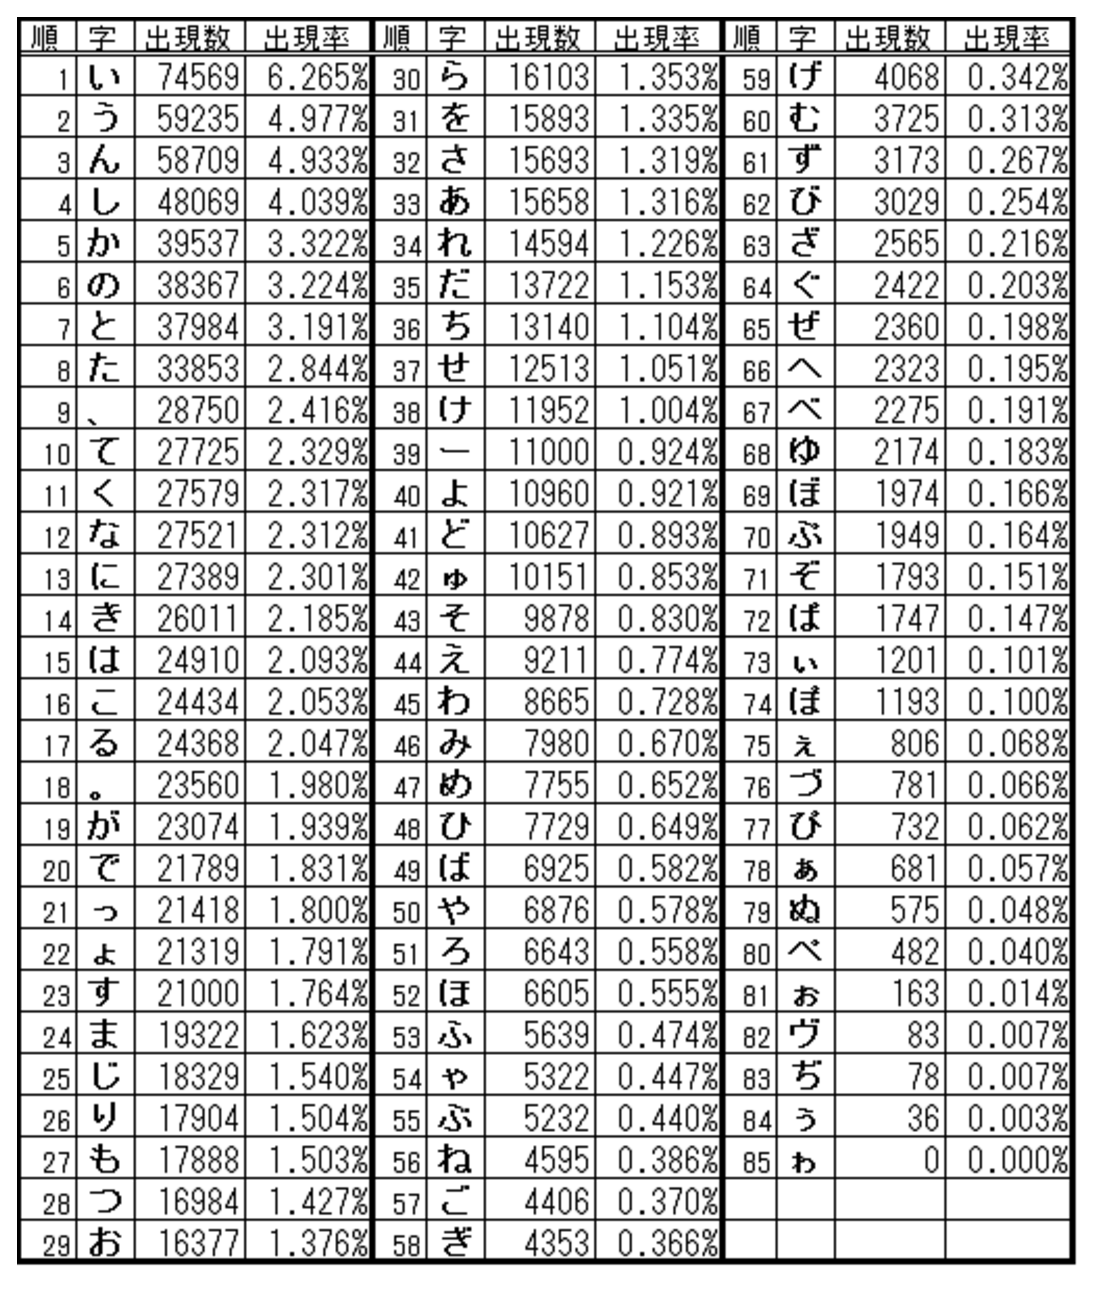
\includegraphics[width=14cm,clip]{res_kouy/1gram.eps}
 \end{center}
 \caption{����100�������̂��ȏo����}
 \label{1gram}
\end{figure*}

���̂悤�ɁA���Ȃ̏o�����͂��Ȃɂ���đ傫���قȂ�܂��B���������āA�o���񐔏�ʂ̂��Ȃ��A�L�[�{�[�h�̑ł��₷���L�[�ɔz�u����΁A�����悭���͂��邱�Ƃ��ł���悤�ɂȂ�܂��B�ł́A�L�[�{�[�h�̑ł��₷���L�[�͂ǂ̃L�[�ł��傤���H

�L�[�{�[�h�̃L�[��łŽw�͕Ў�ɂ‚�5�{����܂��B���̂����e�w�̓L�[�{�[�h�ʼn��i�̃L�[��S�����邷��̂łƂ肠���������܂��B�����L�[��łŽw�͐l�����w�A���w�A��w�A���w��4�{�ł��B���̒��ŃL�[��ł��₷���w�͂ǂ̎w�ł��傤���H�@�l�����w�⒆�w�͓������₷���A�͂�����̂őł��₷���w�ł��B�t�ɁA���w���w�͎v���悤�ɓ��������A���₷���̂őł��ɂ����w�ł��傤�B

�܂��A�L�[�{�[�h�̕����L�[��4�i�ɂ킽���Ĕz�u����Ă��܂��B�u�ŏ�i�v�i�L�[�̍����珇��\key{1}\key{2}\key{3}\key{4}\key{5}�c�c�ƕ���ł���i�j�A�u��i�v�i������\key{Q}\key{W}\key{E}\key{R}\key{T}�c�c�j�A�u�z�[���i�i���i�j�v�i������\key{A}\key{S}\key{D}\key{F}\key{G}�c�c�j�A�u���i�v�i������\key{Z}\key{X}\key{C}\key{V}\key{B}�c�c�j��4�i�ł��B���̂����ł��ł��₷���L�[�̒i�́A��͂�w�𓮂����Ȃ��Ă��ރz�[���i�̃L�[�ł��傤�B����1�i�w�𓮂����K�v�������i�����i�B�ŏ�i��2�i�w�𓮂����K�v������̂ōł��ł��ɂ����i�ł��B

����ɁA�L�[�̉��̃Y����w�̒����Ȃǂɂ���đł��₷�����ς��܂��B�}\ref{key_utiyasusa}�͂킽�����v���e�L�[�̑ł��₷�������������̂ł��B�ł��₷�����Ɂu���A���A���A�~�v�ł��B
���̕\�́��⁛�̂‚����L�[�𑽂��g���A����~�̂‚����L�[�����܂�g��Ȃ��悤�ɂ���΁A�����悭���͂��邱�Ƃ��ł��܂��B


\begin{figure*}
 \begin{center}
   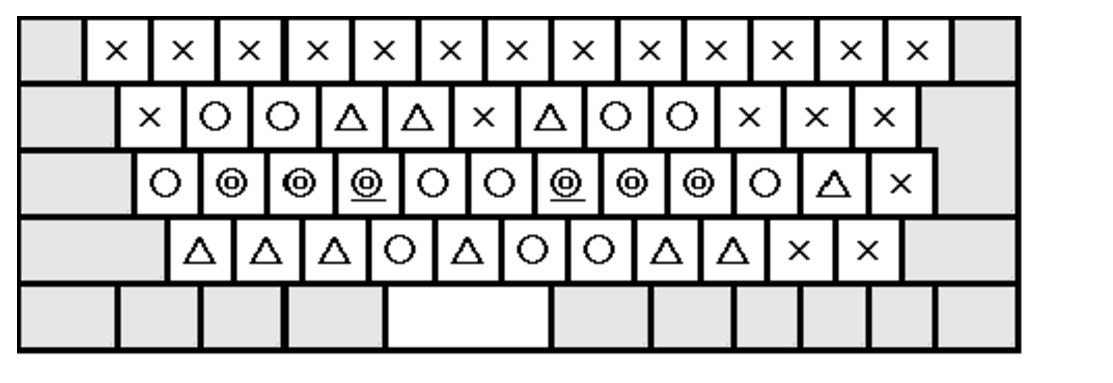
\includegraphics[width=14cm,clip]{res_kouy/key_utiyasusa.eps}
 \end{center}
 \caption{�e�L�[�̑ł��₷��}
 \label{key_utiyasusa}
\end{figure*}

���̂悤�ɁA�V�z��͓��{��ƃL�[�{�[�h�𕪐͂��č��܂��B�V�z��ōl������v�f���g�����̏o�����h�Ɓg�L�[�̑ł��₷���h�Ƃ���2��ނ��Љ�܂������A���ɂ�2�����ȏ�ŘA�����ďo�����邱�Ƃ������A�Ȃ�i�Ⴆ�΁A�u�傤�v�u�Ă��v�u�����v�Ȃǂ͏o�����������j��A�ǂ��o������t���[�Y�i�u�܂��B�v�u�Ƃ����v�Ȃǂ͏o�����������j���l�����܂��B�܂��A1�L�[�ł̑ł��₷���̂ق��ɁA�A�����ăL�[��łꍇ�̑ł��₷�����l�����܂��i�Ⴆ�΁A\key{K}\key{J}�Ƃ����L�[�̘A���͔��ɑł��₷���B\key{M}\key{U}�̂悤�ɓ����w�ʼn����L�[�𑱂��đłƒL�[�̘A���͑ł��ɂ����j�B

�}\ref{dakensuu_ro-maji}�`\ref{dakensuu_keinarabe}�́A�}\ref{1gram}�̃f�[�^���g�p���āA1�����i���ȂŐ����āj�̕��͂���͂����ꍇ�Ɋe�L�[������Ō����邩��z��ʂɎ��������̂ł�\footnote{�}���̃L�[�{�[�h�O�̐����̈Ӗ��F���̏�i�͏��w�E��w�E���w�E�l�����w�̑Ō����A���̉��i�͏�i�̍��v�A�E�͍ŏ�i�E��i�E���i�E���i�̑Ō����A�E���̏�i�͒ʏ�̃V�t�g�⓯���Ō��V�t�g��0�Ō��Ɛ������ꍇ�̑Ō����A�E���̉��i�͒ʏ�̃V�t�g�⓯���Ō��V�t�g��1�Ō��Ɛ������ꍇ�̑Ō����B}�B�}�����Ă��������ƁA�}\ref{dakensuu_ro-maji}�i���[�}�����́j�A�}\ref{dakensuu_JIS-kana}�i���ȓ��́j�ɔ�ׁA�}\ref{dakensuu_NICOLA}�`\ref{dakensuu_keinarabe}�̐V�z��3��i�e�w�V�t�g�A���z��A�����Ȃ�ׁj�̓z�[���|�W�V�����̃L�[�𑽂��g���̂��킩��Ǝv���܂��B

���{��ŗǂ��o�Ă��镶����ł��₷���L�[�œ��͂ł���B������V�z��͑ł��₷���̂ł��B

\begin{figure*}
 \begin{center}
   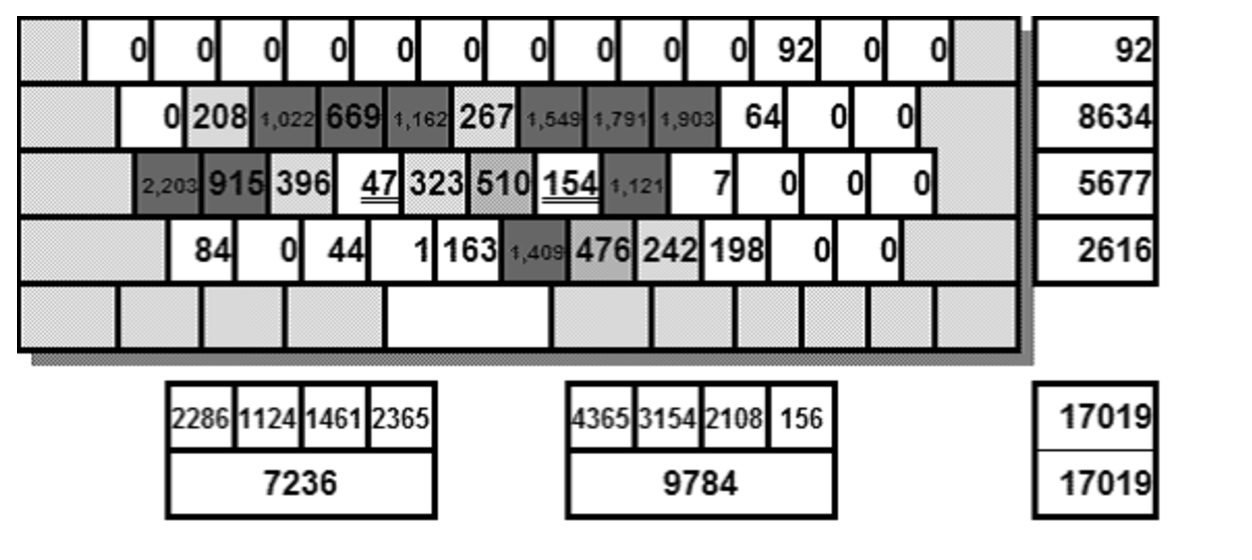
\includegraphics[width=14cm,clip]{res_kouy/dakensuu_ro-maji.eps}
 \end{center}
 \caption{1�����̕��͂���͂����ꍇ�̑Ō����@���[�}������}
 \label{dakensuu_ro-maji}
\end{figure*}

\begin{figure*}
 \begin{center}
   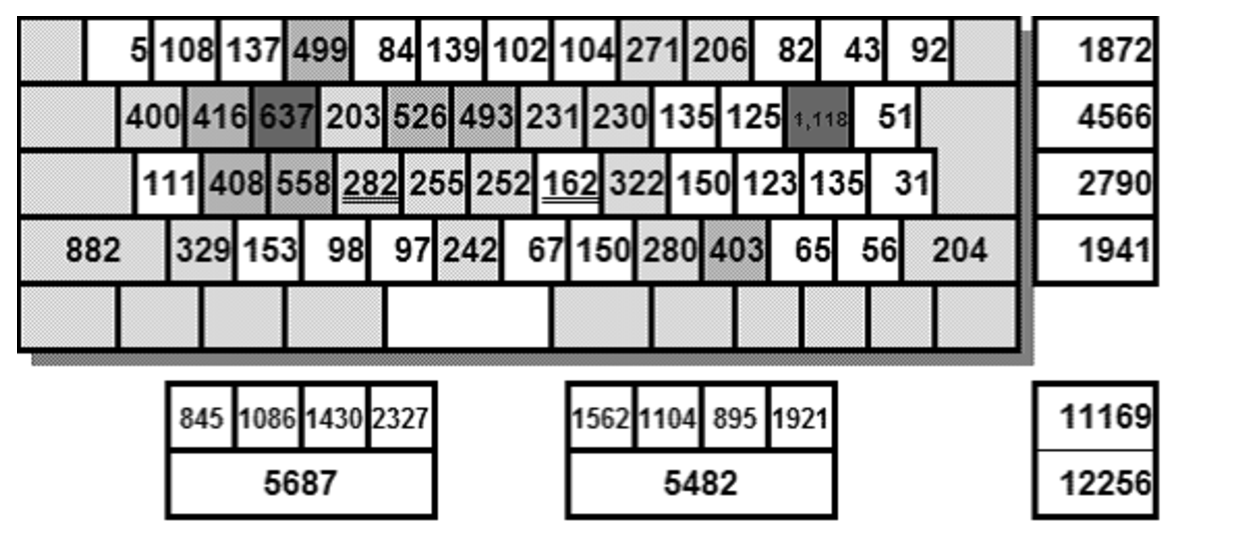
\includegraphics[width=14cm,clip]{res_kouy/dakensuu_JIS-kana.eps}
 \end{center}
 \caption{1�����̕��͂���͂����ꍇ�̑Ō����@���ȓ���}
 \label{dakensuu_JIS-kana}
\end{figure*}

\begin{figure*}
 \begin{center}
   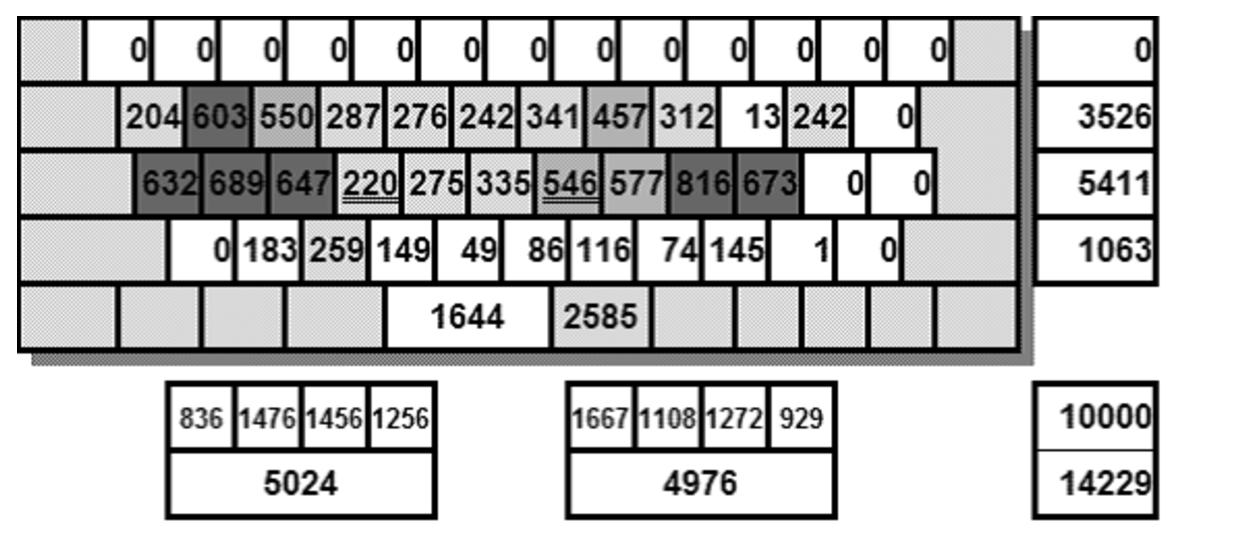
\includegraphics[width=14cm,clip]{res_kouy/dakensuu_NICOLA.eps}
 \end{center}
 \caption{1�����̕��͂���͂����ꍇ�̑Ō����@�e�w�V�t�g�iNICOLA�j}
 \label{dakensuu_NICOLA}
\end{figure*}

\begin{figure*}
 \begin{center}
   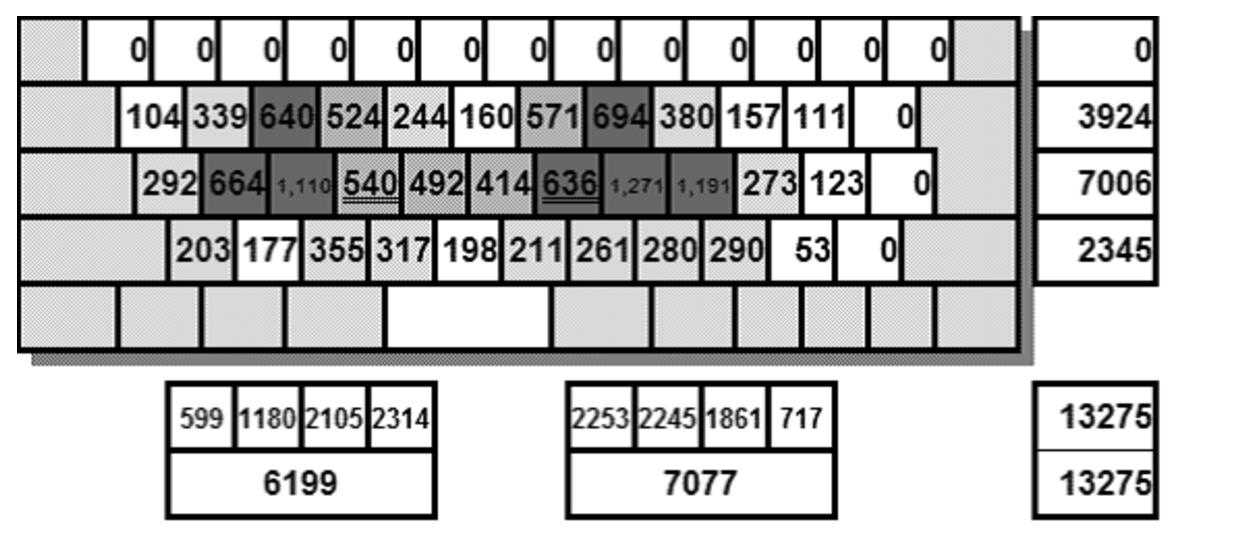
\includegraphics[width=14cm,clip]{res_kouy/dakensuu_tuki2-263.eps}
 \end{center}
 \caption{1�����̕��͂���͂����ꍇ�̑Ō����@���z��2-263��}
 \label{dakensuu_tuki2-263}
\end{figure*}

\begin{figure*}
 \begin{center}
   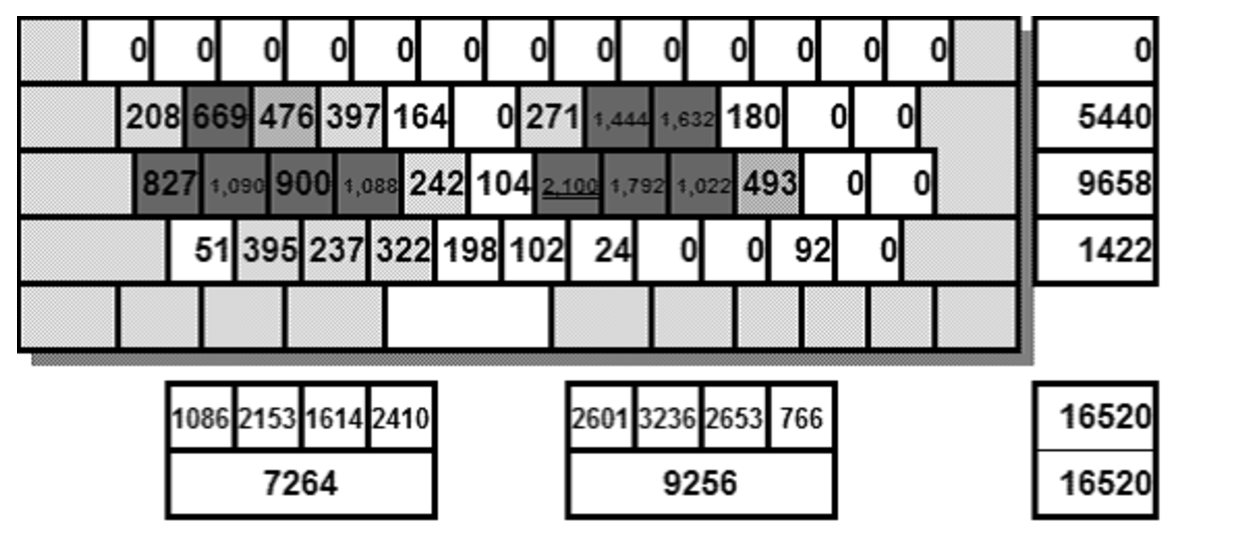
\includegraphics[width=14cm,clip]{res_kouy/dakensuu_keinarabe.eps}
 \end{center}
 \caption{1�����̕��͂���͂����ꍇ�̑Ō����@�����Ȃ��}
 \label{dakensuu_keinarabe}
\end{figure*}

\section{�Ȃ����A�V�z�񂩁H}

�V�z�񂪗D��Ă���ƌ����Ă��A�����p�\�R�����C���^�[�l�b�g������I�ɐG��鐢�̒��B���[�}�����͂Ɋ���Ă��ĉ��̕s�s�����Ȃ��g���Ă���̂ɁA������V�z��Ȃ�āc�c�Ǝv���������邩������܂���B

�������A�p�\�R���ƃC���^�[�l�b�g�����y�����������炱���A�V�z��͒a�����A�g���₷���Ȃ����ƌ�����̂ł��B�u������V�z��v�ł͂Ȃ��u�������V�z��v�Ȃ̂ł��B

\subsection{���܎g���Ă���p�\�R���ŐV�z����g����悤�ɂȂ���}

1980�N�ォ��1990�N��ɂ����āA�p�\�R�������y����O�ɁA���[�v����p�@�����y���Ă������オ����܂����B���[�v����p�@�̎���̔z��̑I���́A���̃��[�v���ɓ��ڂ���Ă���z����g����������܂���ł����B�����̃��[�v���ł̓��[�}�����͂Ƃ��ȓ��͂������ڂ���Ă��܂���ł����̂ŁA�g�p�ł���z��͎����ケ��2��ނɌ��肳��Ă����̂ł��B

���������[�}�����͂Ƃ��ȓ��͈ȊO�ɁA�e�w�V�t�g�iNICOLA�j��VJIS�z��Ƃ������u�V�z��v�͑��݂��Ă��܂����B�������A�e�w�V�t�g���g�����Ǝv������x�m�ʂ�OASYS���A�VJIS�z����g�����Ǝv�����炻�ꂪ���ڂ���Ă���ꕔ�̋@����w�����邵������܂���ł����B�܂��Ă�A�����ŃI���W�i���̔z������Ȃǖ����ꂾ��������ł��B

���݂Ȃ�A�w�������̃p�\�R���Ɏg�������V�z�񂪓��ڂ���Ă��Ȃ��Ă��A���Ƃ���lj����Ď������邱�Ƃ��ł��܂��B

�z�����������\�t�g�E�F�A���g�p����ƁA���g���Ă���p�\�R���A���g���Ă���L�[�{�[�h�̂܂܂ŐV�z����g�p���邱�Ƃ��ł��܂��B���̂悤�ȐV�z�����������\�t�g�E�F�A�̂��Ƃ��u�z��G�~�����[�^�v�ƌĂт܂��i�ȉ��A�P�ɃG�~�����[�^�Ƃ������܂��j�B�G�~�����[�^�͂��܂��܂Ȏ�ނ̕�������A�����Ŏg�����Ƃ��ł�����̂�����܂��B�܂��A�C���^�[�l�b�g��ʂ��ă_�E�����[�h�ł���̂ŁA����ł��ȒP�ɓ���ł��܂��B����ɁA�ꕔ�̐V�z��́A�G�~�����[�^���g���܂ł��Ȃ��AIME���g���Ď����ł�����AOS�ɍŏ����瓋�ڂ���Ă�����̂�����܂��B

�V�z��𓱓����邽�߂̃n�[�h���́A�̂ɔ�ׂ͂邩�ɒႭ�Ȃ����̂ł��B

\subsection{���l�Ȕz�񂪐��܂�Ă���}

�p�\�R���ƃC���^�[�l�b�g�ɂ��V�z�񂪎󂯂����b�́A���ꂾ���ł͂���܂���B

�O�q�̒ʂ�A���݂ł̓G�~�����[�^���g���ΊȒP�ɐV�z����������邱�Ƃ��ł��܂��B�����ăG�~�����[�^�̑����́A�����̔z�u�����R�ɓ���ւ�����Ƃ����@�\������Ă��܂��B���̋@�\�ɂ��A���‚Ă͖����ꂾ�����u�����ŃI���W�i���̔z������v���Ƃ��ł���悤�ɂȂ�܂����B�u��������΂����Ɨǂ��Ȃ�v�Ǝv���_���C��������A�ꂩ��܂������V�����z������Ƃ������Ƃ��A�ȒP�ɂł���悤�ɂȂ����̂ł��B

����ɂ��A2000�N�O�ォ�猻�݂ɂ����āA�������̐V�z�񂪐��ݏo�����悤�ɂȂ�܂����B�����͌l�ɂ���č��ꂽ���̂ł����A�C���^�[�l�b�g����炵���A�l�b�g��Ɍ��J����A�����̐l�̈ӌ���������ď������C�����č��ꂽ�V�z�������܂��B

�V�z������ɂ́A��ɂ��������ʂ���{��̕��͂��s�Œ��ł��B���‚ẮA���{��̕��͂��̏W���āA�������͂���Ƃ����̂͑�ςȎ�Ԃ��������Ƃł����B

�������A���ꂳ�����p�\�R���ƃC���^�[�l�b�g���������Ă��܂��܂����B���݂ł́A�z�����邽�߂ɕK�v�ȓ��{��̃f�[�^�̓C���^�[�l�b�g��Ō��J����Ă��܂��B���‚Ă͌l�ł͂ƂĂ���ɕ����Ȃ������悤�ȃf�[�^���A�ȒP�Ɏ�ɓ���邱�Ƃ��ł���̂ł��B����ɕK�v�Ȃ�A�����œ��{��𕪐͂��邱�Ƃ��ł��܂��B���̂��߂ɕK�v�ȕ��͉�̓c�[�����A�l�b�g����_�E�����[�h�ł���̂ł��B

���炽�ȐV�z�񂪎��X�ƒa���������Ƃɂ��A�V�z��̑I�����͑傫���L����܂����B���‚Ă̓��[�}�����͂₩�ȓ��͈ȊO�̔z��ƌ����΁A�e�w�V�t�g���炢�����I����������܂���ł����B���݂ł́A�e�w���V�t�g�Ƃ���z��A���w���V�t�g�Ƃ���z��A�����Ō����g���z��E�g��Ȃ��z��A�o���₷���ɏd�_��u�����z��ȂǁA���ꂼ��ɗD�ꂽ�����̂���z�񂪑������ݏo����Ă��܂��B21���I�ɓ����Ă���10�N�ȏオ�o���A�V�z��͂܂���\ruby{�S��㇗�}{�Ђ������傤���}�B���낻���v�ȃA�C�f�A���o�s�����A�~�n�����}�����ƌ�����Ǝv���܂��B

���Ȃ�A���Ȃ����C�ɂ���V�z�񂪂����ƌ��‚���͂��ł��B

\section{���Ȃ�V�z�񂾂��Ċo������}

�V�z�񂪑䓪���Ă����̂͂킩��������ǁA���łɃ��[�}�����͂Ɋ���Ă��邵�A���܂�����͕��@��ς���C�ɂ͂Ȃ�Ȃ��A�Ǝv������������������܂���B

���߂ăp�\�R����G�����Ƃ��A�L�[�{�[�h�̓��͂ɋ�킵���L���͒N�ɂł�����Ǝv���܂��B�ǂ��ɉ��̃L�[������̂��܂�����������Ȃ��B1�������͂��邲�ƂɃL�[�{�[�h����ړI�̃L�[����ˆ�’T���o���B�u����ɂ��́v��1����͂��邾���ł����J�B�V�z����g���Ƃ���ƁA�܂����̌o�����J��Ԃ��Ȃ���΂Ȃ�Ȃ��̂��B��������ȋ�J�͂܂��҂��ƁA�Ǝv���C�������킩��Ȃ��ł͂���܂���B

�������A�m���ɐV�z����g�����Ȃ��ɂ͈��̗��K���K�v�ł����A�V�z��̏K���͂���قǑ�ςȂ��Ƃł͂���܂���B���߂ăp�\�R���ɐG�ꂽ�Ƃ��Ƀ��[�}�����͂��o�����Ƃ��Ɣ�ׂ�΁A�����ƊȒP�Ɋo���邱�Ƃ��ł��܂��B

\subsection{�L�[�{�[�h�Ɋ���Ă���}

�V�z��̏K�����ȒP�ȑ��̗��R�́A���łɃL�[�{�[�h���̂ɂ͊���Ă���Ƃ������Ƃł��B�݂Ȃ���̓��[�}�����͂Ȃ肩�ȓ��͂Ȃ�ŁA�L�[�{�[�h�ŕ�������͂���Ƃ������Ǝ��̂́\�\���ꂼ��ɒ��x�̍��͂���ł��傤���\�\�K������Ă���Ǝv���܂��B

�p�\�R���ɐG�ꂽ�����A�L�[�{�[�h�ɏ��߂ĐG�ꂽ�Ƃ��ɕ������͂ɋ�J�����̂͂Ȃ��ł��傤���H�@�������A�ǂ̃L�[���ǂ��ɔz�u����Ă��邩������Ȃ��Ƃ������R������ł��傤�B�������A�L�[�{�[�h���̂Ɋ���Ă��Ȃ����Ƃ��傫�ȗ��R�������͂��ł��B�������Ƃ��Ă���L�[��ڂŌ��āA�ʒu���m�F���Ȃ��Ƃ��̃L�[�������Ȃ��B�L�[�{�[�h�����Ȃ��őłƂ��Ƃ��Ă��A�ǂ̎w���ǂ̂��炢�������΂ǂ̃L�[��������̂��A�ǂ̂��炢�̋����ʼn����΂����̂��A�܂������������‚��Ȃ��B�������‚���ʼn����Ă��Ȃ�������A�����Ă��Ȃ��͂��̂̃L�[��������Ă����肷��B�������肷��ƃL�[�̊ԂɎw��������2�ƒL�[�������Ă��܂��c�c�B�ŏ��͂���ȏ�Ԃ������Ǝv���܂��B

�L�[�{�[�h�Ɋ��ꂽ���Ȃ�A����Ȃ��Ƃ͂���܂���B�L�[�{�[�h�ɑ΂��銴�o�͂��łɐg�ɂ‚��Ă��܂��B�ǂ̃L�[��łĂ΂����̂�������΁A�ړI�̃L�[��ł‚��Ƃ͊ȒP�ɂł��܂��B���̊��o�͐V�z��ł����̂܂܎g�����Ƃ��ł��܂��B

����ɁA���łɃp�\�R���̑���Ɋ���Ă���Ƃ������R������܂��B�p�\�R���ɐG�ꂽ�����́A�ǂ̃L�[���������牽���N����̂��\���ł��Ȃ���Ԃł��B1�ƒL�[�������ԈႦ�������Œv���I�Ȏ��Ԃ��N���邩������Ȃ��B�Ԉ�����L�[���������Ƃ��A�ǂ�����ΏC���ł���̂����킩��Ȃ��B������ԈႦ�����Ȃ��B����ƁA���������m�F���Ȃ��ƃL�[�������Ȃ����A��������ԈႦ��ƏC���Ɏ��Ԃ�������܂��B����ł͂Ȃ��Ȃ����͂��i�܂��A�Ȃ��Ȃ�����邱�Ƃ��ł��܂���B

���Ȃ炻��Ȃ��Ƃ͂���܂���B�Ƃ肠�����J�`���J�`���Ɠ��͂��āA�Ԉ���Ă����璼���Ηǂ������̂��Ƃł��B�ǂ�ǂ�L�[��ł��Ăǂ�ǂ�C�����Ă����΁A�����Ɋ���邱�Ƃ��ł��܂��B

���߂ɔz����o�����Ƃ��Ƃ����̂́A���͔z��ȊO�̂��Ƃ������Ɋo���Ă����̂ł��B���Ȃ�A�L�[�{�[�h�ɂ͊���Ă��邵�A�p�\�R���̑����������܂��B�z����o���邱�Ƃ����ɏW���ł���̂ł��B

\subsection{�ł��₷���L�[�𑽂��g��}

�V�z��̏K�����ȒP�Ȃ�����‚̗��R�́A�V�z��͑ł��₷���L�[�𑽂��g���Ƃ������Ƃł��B�L�[�{�[�h�̃L�[�̒��ɂ́A�ł‚̂��ȒP�ȃL�[�Ɠ���L�[������܂��B�ł‚̂��ȒP�ȃL�[�𑽂��g���قǏK�����₷���Ȃ�܂��B

�ł́A�ł‚̂��ȒP�ȃL�[�Ƃ͂ǂ̃L�[�ł��傤���H�@�z�[���|�W�V�����ł͂Ȃ��L�[��łꍇ�́A�w�����̃L�[�̏�ɐ��m�ɓ������Ȃ���΂����܂��񂩂�A�ł‚̂�����Ȃ�܂��B�܂��A���w�͗͂��キ�ق��̎w�ɔ�ׂĎg���ɂ����̂ŁA���m�ɃL�[��ł‚̂�����w�ł��B�t�ɁA�w���L�[�̏ォ�瓮�������ɍςރz�[���|�W�V�����̃L�[���A�������₷���l�����w�E���w�E��w���g���đłꍇ�́A�ȒP�ɑł‚��Ƃ��ł��܂��B
����āA�ł��ł‚̂��ȒP�ȃL�[�́A�l�����w�E���w�E��w�̃z�[���|�W�V�����̃L�[�A��̓I�ɂ�\key{S}\key{D}\key{F}�A\key{J}\key{K}\key{L}��6�L�[�ƂȂ�܂��B

�������A���[�}�����͂ł͂����̃L�[�̎g�p���͂��܂荂������܂���B���[�}�����͂ōł��悭�g���L�[�́A�ꉹ�L�[�A���Ȃ킿\key{A}\key{I}\key{U}\key{E}\key{O}��5�L�[�ł��B����5�L�[�́A��قNj������ł‚̂��ȒP��6�L�[�ɂ͈�‚��܂܂�Ă��܂���B�‚܂胍�[�}�����͂́A�ł‚̂��ȒP�ȃL�[�����܂�g�킸�A������ł‚̂�����L�[��p�ɂɎg���z��Ȃ̂ł��B����ł͏K��������Ȃ�̂��K�R�ł��B

���ȓ��͂��A�ł‚̂��ȒP�ȃL�[�𑽂��g���Ƃ͌����Ȃ��z��ł��B�z�[���i����i�̕����g�p��������������A�ŏ�i�ɂ��g�p�������Ȃ荂���L�[����������A���|�I�ɏo�������������_���z�[���|�W�V��������O�ꂽ�A���������w���S������L�[�ɔz�u����Ă����肵�܂��B�w���z�[���|�W�V�������痣��ĉ����̃L�[��ł��ɍs���@������̂ł�����A���G�Ȏw�̓����������A��x���A�b�v���܂��B

�w�𓮂����Ȃ��čςރz�[���|�W�V�����̃L�[�𑽂��g���A�����w�ňقȂ�L�[�𑱂��đł‚悤�ȕ��G�ȓ���͂ł��邾�����Ȃ��B����Ȕz��Ȃ�A�K������̂͂����ƊȒP�Ȃ��ƂɂȂ�܂��B

�V�z��́A���{��ő����o�����镶������͂��₷���悤�ɔz�u���Ă��܂��B�K�R�I�ɁA�ł��₷���L�[�̎g�p���������Ȃ�A���G�Ȏw�̓��������Ȃ��Ȃ�܂��B����͓��͂��������I�ɂł���悤�ɍH�v�������ʂł����A���̂悤�Ȕz��́\�\�K��������Ɍ����I�ɓ��͂ł��邾���łȂ��\�\�K�����邱�Ǝ��̂��Ղ����Ȃ�̂ł��B

\section{�V�z��FAQ}

\subsection{�V�z������܎g���Ă���p�\�R���Ŏg����H}

\subsubsection*{�y����z}

�V�z����g���ɂ́A�V���Ƀp�\�R����L�[�{�[�h�Ȃǂ𔃂��K�v������̂ł����H�@�V�z������܎g���Ă���p�\�R���Ŏg���ɂ͂ǂ�������悢�ł����H

\subsubsection*{�y�񓚁z}

�z���OS�ɂ���Ă��܂��܂Ȏ������@������܂����A�z��G�~�����[�^�ƌĂ΂��\�t�g�E�F�A���g���ĐV�z�����������̂��ȒP�ȕ��@�ł��B�G�~�����[�^���g���΁A���܎g���Ă���p�\�R���A�L�[�{�[�h���g�p�����܂ܐV�z����g�p���邱�Ƃ��ł��܂��B�V���Ƀp�\�R����L�[�{�[�h���w������K�v�͂���܂���B

�G�~�����[�^�͂��܂��܂Ȏ�ނ̂��̂����݂��܂��B�ȉ��ɑ�\�I�Ȕz��G�~�����[�^�������܂��B

\begin{itemize}
 \item �w�P�x�q���x�i�V�F�A�E�F�A�j
 \item �wDvorakJ�x�i�t���[�\�t�g�j
 \item �w��܂Ԃ��x�i�t���[�\�t�g�j
\end{itemize}

�܂��A�z��G�~�����[�^�̂ق��ɁA�L�[�J�X�^�}�C�Y�\�t�g�i�L�[�o�C���h�ύX�\�t�g�j�ƌĂ΂��W�������̃\�t�g������܂��B�z��G�~�����[�^����ɃL�[���������Ƃ��ɓ��͂���镶����ύX����̂ɑ΂��A�L�[�J�X�^�}�C�Y�\�t�g�̓L�[�̋@�\���̂��̂�ύX���܂��B�������A�z��G�~�����[�^�ŃL�[�̋@�\��ύX�ł�����A�L�[�J�X�^�}�C�Y�\�t�g�ł����͂���镶����ύX�ł�����̂�����̂ŁA���̋��ڂ͂����܂��ł��B�ȉ��A��\�I�ȃL�[�J�X�^�}�C�Y�\�t�g�������܂��B

\begin{itemize}
 \item �w�̂ǂ��x�i�V�F�A�E�F�A�j
 \item �wYet Another Mado tsukai no Yuutsu�x�i�t���[�\�t�g�j
 \item �w���g���̗J�T�x�i�t���[�\�t�g�j
 \item �wKeySwap for XP�x�i�t���[�\�t�g�j
 \item �wKeyRemap4MacBook�x�i�t���[�\�t�g�j
\end{itemize}


\subsection{�ق��̃p�\�R�����g�����ɍ���Ȃ��ł����H}

\subsubsection*{�y����z}

�V�z����g���ɂ̓G�~�����[�^�Ȃǂ��g�p����K�v�����邻���ł����A��������Ǝ����̃p�\�R�����g���Ƃ��͂悢�ł����A�ق��̃p�\�R�����g���Ƃ��ɐV�z����g�����Ƃ��ł��Ȃ��̂ł͂Ȃ��ł����H�@����͍���܂��񂩁H

\subsubsection*{�y�񓚁z}

�V�z�����������ɂ̓G�~�����[�^�Ȃǂ��g�p����K�v������܂����A�G�~�����[�^��USB�������Ȃǂɓ���Ď����^�ׂ�^�C�v�̂��̂�����܂��B����𗘗p����΁A�ǂ̃p�\�R���ł��V�z��𗘗p���邱�Ƃ͉”\�ł��B

�܂��A�V�z����g���Ȃ��󋵂ł́A���̂Ƃ��������[�}�����͂��g�p���邱�Ƃɂ���Ζ�肠��܂���B����FAQ�������������B

\subsection{���[�}�����͂ƐV�z��𕹗p�ł��܂����H}

\subsubsection*{�y����z}

�V�z����o���Ă��A���[�}�����͂��g�����Ƃ͂ł��܂����H�@���[�}�����͂�Y��Ă��܂����Ƃ͂���܂��񂩁H

\subsubsection*{�y�񓚁z}

�V�z����o���Ă��A���܂܂Ŏg���Ă������[�}�����͂͂��̂܂܎g�����Ƃ��ł��܂��B��x���]�Ԃ̏������o����ƁA���΂炭���]�Ԃɏ��Ȃ����Ԃ������Ă������͖Y��Ȃ��A�Ƃ������ۂɎ��Ă��܂��B

���ہA�V�z����g���Ă���l�̑����́A�K�v������΃��[�}�����͂œ��͂��Ă��܂��B�킽���������̃p�\�R���ȊO�œ��͂���K�v������Ƃ��̓��[�}�����͂��g�p���Ă��܂����A�܂��������Ȃ��g�p�ł��܂��B

\subsection{���[�}�����͂̓A���t�@�x�b�g�̔z�u���g���邩��ǂ��̂ł́H}

\subsubsection*{�y����z}

�p�\�R���̕������͂ł́A���Ȃ̓��͂̂ق��ɃA���t�@�x�b�g�̓��͂��g���܂��B���[�}�����͂Ȃ�A���t�@�x�b�g�̔z��1�‚ł��Ȃ��A���t�@�x�b�g�����͂ł���̂ŁA��͂胍�[�}�����͂��g���̂������I�ł͂Ȃ��ł��傤���H

\subsubsection*{�y�񓚁z}

���[�}�����͂̏K����ʂ��ăA���t�@�x�b�g�̔z�u��������x�o���邱�Ƃ��ł��܂��̂ŁA�p�\�R�����S�҂̒i�K�A�‚܂肩�Ȃ̓��͂��A���t�@�x�b�g�̓��͂��o�����ĂȂ��Ƃ����i�K�ł́A�m���Ƀ����b�g�͂���Ǝv���܂��B���߂ăp�\�R���ɐG�����l�����[�}�����͂��o����Ƃ����̂́A���̍�����������Ǝv���܂��B

�������A����ȏ�̒i�K�ɂȂ�ƁA���[�}�����͂�ʂ��ăA���t�@�x�b�g�̓��͂���K�ł���Ƃ������ʂ͂قƂ�ǖ����Ȃ��Ă��܂��B���[�}�����͂Ɋ���Ă���ƁA���[�}�����͂�����ۂł��A���t�@�x�b�g���قƂ�Ljӎ����Ȃ��œ��͂ł���悤�ɂȂ�܂��B�u���v�Ɠ��͂���Ƃ��ɁA\key{K}��\key{A}��ł‚ƈӎ�����̂ł͂Ȃ��A�P�Ɂu���v�̓��͂ɕK�v��2�‚̃L�[��ł‚Ƃ������o�ɂȂ�܂��B�A���t�@�x�b�g���ӎ����Ȃ��̂ł�����A���[�}�����͂��g�������Ă��A�A���t�@�x�b�g�̓��͂���B���邱�Ƃ͂���܂���B�p����͉͂p����͂ŁA���[�}�����͂Ƃ͕ʂɏK������K�v������܂��B

����āA�A���t�@�x�b�g�̓��͂��g���Ƃ��Ă��A���[�}�����͂��L���Ƃ������Ƃ͂���܂���B���Ȃ̓��͕��@�̓A���t�@�x�b�g�̓��͂Ƃ͐؂藣���āA�����܂Łg���Ȃ̓��́h�����₷�����@��I�ԕ��������I���Ǝv���܂��B

\subsection{�V�z����o����̂ɂǂꂭ�炢�̎��Ԃ�������܂����H}

\subsubsection*{�y����z}

�V�z����g���Ă�����x���炷����͂ł���悤�ɂȂ�܂ŁA�ǂꂭ�炢�̎��Ԃ�������܂����H

\subsubsection*{�y�񓚁z}

���K���@��A�ǂꂭ�炢�W�����ė��K�ł��邩�A�o����V�z��̓�x�Ȃǂɂ���ĈقȂ�܂����A����܂ł̐V�z����o�����l�̑̌��k�ɂ���2�T�ԁ`2�����قǂ̂悤�ł��B

�V�z����K������܂ł́A�傫��2�‚̃X�e�b�v�ɕ�����܂��B1�–ڂ��u���̃X�e�b�v�v�\�\�z��}�𓪂̒��ɓ����\�\�A2�–ڂ��u�w�̃X�e�b�v�v�\�\���镶������͂��悤�Ǝv�����Ƃ��Ɏw���u���ɂ��̃L�[�łĂ�悤�ɂȂ�\�\�A�ł��B�u���̃X�e�b�v�v�ɂ�������Ԃ͔z��ɂ���đ傫���قȂ�܂��B�܏\�����ɕ��ׂ��悤�ȒP���Ȕz��Ȃ炷���ɂł��o������ł��傤�B�o����v�f�������Ȃ�قNJo����̂�����Ȃ�܂��B�l�l�̋L���͂���K�̏W���x�ɂ���Ă��قȂ�ł��傤�B�u�w�̃X�e�b�v�v�Ɋւ��ẮA�z��̍��͂���قǂ���܂���B�P���Ȕz��ł����Ă��w�����������Ȃ�悤�ɂȂ�܂łɂ͂�����x�̗��K���K�v�ł��B����΂���͂Ƃɂ����g���Ċ���邵���Ȃ��悤�ł��B

�ŏ��͎w�������Ȃ��ċ�J����Ǝv���܂����A�������͑��x���オ��Γ������K���Ԃō��܂ł�葽���̗��K���ł��邱�ƂɂȂ܂��B����Ɨ��K�������ǂ��Ȃ�A���̌��ʓ��͑��x���オ���āA����ɗ��K�������ǂ��Ȃ�c�c�Ɖ����x�I�ɓ��͑��x���オ���Ă����܂��B�����Ȃ�ΐV�z��K���ԋ߂ƌ�����ł��傤�B

�V�z����o����R�c����B�V�z��ł͗ǂ��o�����邩�Ȃ͑ł��₷���L�[�ɔz�u����Ă��܂��B���������āA�ǂ��o�����邩�Ȃ�T���Ƃ��͑ł��₷���L�[�A���܂�o�����Ȃ����Ȃ�T���Ƃ��͑ł��ɂ����L�[��T���ƌ��‚���₷���Ȃ�܂��B

�ǂ̂��Ȃ��ǂ��o������̂��\�\��Ɍf�ڂ����}1-1�̒ʂ�ł����\�\������Ȃ��Ǝv����������܂���B���������ςɌ����ƁA�܏\���\�̍ŏ��̕��ɏo�Ă��邩�Ȃ͗ǂ��o�Ă��܂��i�������A�u��v�͍ŕp�o���Ȃ̈�‚ł��j�B���������ڂ��������ƁA���s�`���s�͂قڂ��ׂďo������ʂ̂��Ȃł��B�ȍs�́u�ȁv�u�Ɂv�Ɓu�́v�A�͍s�́u�́v�����B���̂��炢�܂ł��o�����������ƌ����邩�Ȃł��B��O�͂���܂����A���ꂾ���ł��V�z����o���鏕���ɂ͂Ȃ�Ǝv���܂��B

\subsection{�V�z��̗��K���@�͂ǂ�����΂悢�ł����H}

\subsubsection*{�y����z}

�V�z��̗��K�͂ǂ̂悤�ȕ��@�ōs���΂悢�ł��傤���H

\subsubsection*{�y�񓚁z}

�l�l�ōD�݂�‹��A���K�ɂ������鎞�ԂȂǂ��قȂ�܂��̂ŁA�x�X�g�̕��@�͂��ꂼ��قȂ�Ǝv���܂��B�����ł͂킽�����������߂�����@����Љ�܂��B

�܂��A�z��}���ËL���܂��B���̒i�K�ł͎��ۂɃp�\�R�����g�����������͂͂��܂���B�z��}�����ɏ����Ď��������āA�󂫎��ԂɂƂ��ǂ�����悤�ɂ���Ɗo���₷���Ǝv���܂��B�z��}�����������Ɏ��ɏ����邭�炢�܂Ŋo����ƃx�X�g�ł��B�������A�z��}�������珇�Ԃɓǂ�Ŋo����悤�Ȃ����Ŋo���Ă����܂�Ӗ�������܂���B���ȂƃL�[��1��1�Ŋo����悤�ɐS�����Ă��������B

�z��}���o������A�^�C�s���O�Q�[���ŗ��K���܂��B�w�^�C�v�E�F���x�͋L�^���ڍׂɎc���Ď����̐������m�F�ł���̂ł������߂ł��B�܂����ۂ̕��͓��͂ł͎g�p���܂���B���͂��l����Ƃ����̂͑�ςȍ�Ƃł��B�܂�1����1�������͂���̂���ςȒi�K�ł�����A���͂��l���Ȃ���V�z��̗��K������Ƃ����̂́A��ςȍ�Ƃ𓯎��ɍs�����ƂɂȂ�A�ւ������đ�ςȍ�ƂɂȂ�܂��B�^�C�s���O�Q�[���Ȃ���͂��镶���̓Q�[���̕��Ŏ����I�ɒ񎦂��Ă���܂��̂ŁA�����͔z��̗��K�ɏW�����邱�Ƃ��ł��܂��B

���̍ہA�z��}�����S�Ɋo������܂ł́A�z��������������f�B�X�v���C�̋߂��ɓ\���Ă����Ɨǂ��ł��傤�B�������A���͂ł���Ǝv�����玆�����Ȃ��ŃL�[�������Ă��������B�o���Ă���̂Ɏ������Ă��܂��ƁA���͑��x�Ɏ����Ńu���[�L���|���Ă��܂����ƂɂȂ�A�����ɐ��������܂��B�Ƃ肠�����L�[��ł��āA�Ԉ���Ă�����C������΂悢�̂ł��B

�����Ă�����x�̑��x�œ��͂ł���悤�ɂȂ�����\�\�^�C�v�E�F���Ō����Α������x��E���炢�\�\���ۂ̕��͓��͂ł��g�p���n�߂܂��B

���܏Љ�����K���@�͂����܂ň��ł��B�u�v�����������̓����瑦���퓊���I�v�Ƃ������K���@������܂��B���ꂼ��ŗǂ��Ǝv�����@��I��ł��������B

�܂��A���K�p�\�t�g����K�p�e�L�X�g���p�ӂ���Ă���V�z�������܂��B�Ⴆ�΁A�e�w�V�t�g�iNICOLA�j�ɂ́A�w�e�w�V�t�g���K�x�Ƃ������K�p�̃t���[�\�t�g������܂��B�����𗘗p����̂��ǂ��ł��傤�B

\subsection{�K������܂ł̊ԁA����̕��͓��͍�Ƃ��ǂ�����΂悢�ł��傤���H}

\subsubsection*{�y����z}

�V�z����K������܂ł̊ԁA���͓��͑��x���������ቺ����̂���ɂł��B�ǂ����Ă��߂������ɏ����グ�Ȃ���΂����Ȃ����͂�����܂��B�ǂ�����΂悢�ł����H

\subsubsection*{�y�񓚁z}

������x�W�����ė��K�ł�����Ԃ�����΃x�X�g�ł����A���ۂɂ͓���ꍇ�������Ǝv���܂��B�킽���̈ӌ��ł́A�܂��V�z��ł̓��͑��x�ł͎��ۂ̕��͓��͂Ŏg���ɂ͕s�����Ƃ����ꍇ�́A�������Ă܂ŗ��K���̐V�z����g�p���Ȃ��ŁA���[�}�����͂œ��͂��Ă��ǂ��Ǝv���܂��B���[�}�����͂��g�p��������Ƃ����ĐV�z��̗��K���ʂ�������������Ƃ������Ƃ͂���܂���B

�������A���ۂ̕��͓��͂�����K�v���Ȃ��A�V�z��̗��K�ɏW���ł�����Ԃ��m�ۂł���Ȃ炻�ꂪ���z�ł��B�����x�݂Ȃǂ𗘗p����̂���‚̕��@�ł��傤�B

\section{�������ߐV�z��}

����ł͐V�z�񂪂ǂ̂悤�Ȃ��̂Ȃ̂���̓I�Ɍ��Ă����܂��傤�B�V�z��͎����‹��A�K����x�A�z�񗝘_�Ȃǂɂ��A�������̎�ނ�����܂��B�����ł͂킽�����������߂���V�z���5�Љ�܂��B

\subsection{�e�w�V�t�g�iNICOLA�j}

�e�w�V�t�g�͐V�z��̒��ōł��L���Ȕz��ł��B���[�v����p�@�̎��ォ�瑶�݂���z��ŁA���݂ł������̈��p�҂����܂��B

\begin{figure*}
 \begin{center}
   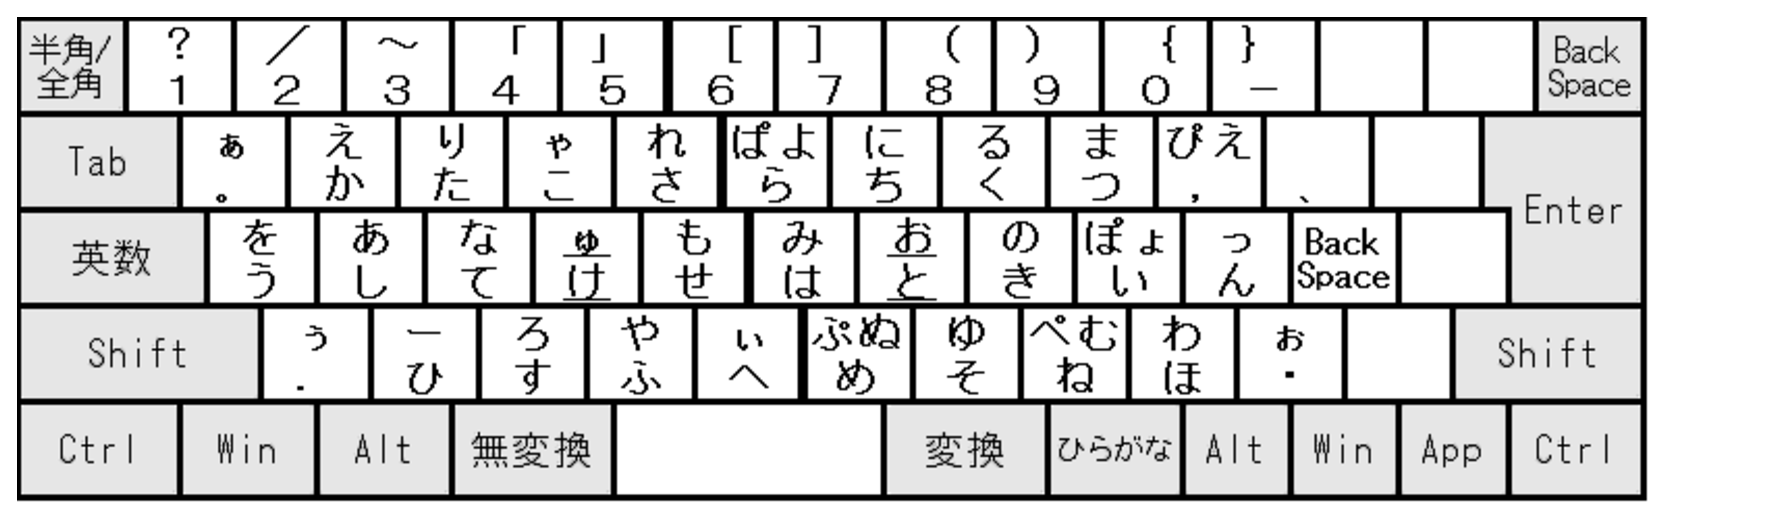
\includegraphics[width=14cm,clip]{res_kouy/NICOLA.eps}
 \end{center}
 \caption{�e�w�V�t�g�iNICOLA�j�z��}}
 \label{NICOLA}
\end{figure*}

\subsubsection*{�e�w���V�t�g�L�[�ɂ���}

�e�w�V�t�g�̍ő�̓����́A�u�e�w�L�[�v���g�p���ĕ�������͂��邱�Ƃł��B

�}\ref{NICOLA}�͐e�w�V�t�g�̔z��}�ł��B1�‚̃L�[��2�‚̕�����������Ă��܂��B�L�[�̉����ɏ����ꂽ�����́A�P�ɂ��̃L�[���������Ƃɂ���ē��͂��܂��i�P�Łj�B�����ăL�[�̏㑤�̕����́A���̃L�[��������Ɠ�����́u�e�w�L�[�v�i�ʏ��\key{���ϊ�}��\key{�X�y�[�X}��\key{�ϊ�}�̂����ꂩ�B���Ƃŏڂ����������܂��j�𓯎��ɉ������Ƃɂ���ē��͂��܂��B�Ⴆ�΁A��i�̍�����2�Ԗڂ̃L�[�i\key{W}�j�ɂ́u���v�Ɓu���v�Ƃ���2��ނ̂��Ȃ�������Ă��܂��B�u���v�Ɠ��͂���Ƃ��́A\key{W}��P�ɉ����܂��B�u���v�Ɠ��͂���Ƃ���\key{W}��\key{���e�w}�𓯎��ɉ����܂��B�܂��A���̃L�[��������Ɣ��΂̎�̐e�w�L�[�𓯎��ɉ������ꍇ�́A�P�łœ��͂ł��邩�Ȃɑ��_���t������������͂��܂��B�Ⴆ��\key{W}��\key{�E�e�w}�𓯎��ɉ����ƁA�u���v�����͂���܂��B���̂悤�ɁA�e�w�V�t�g�ł̓V�t�g���̕�������͂���Ƃ��ɁA�e�w�L�[���g�p���܂��B

���{����͂̍ہA�e�w�S���̃L�[�͂��܂�g���邱�Ƃ̂Ȃ��L�[�ł��B�����ϊ��̂Ƃ��͂�����x�g�p���܂����A���̑��̑���͎g�p���͂���قǍ�������܂���B�p��̏ꍇ�ł��ƃX�y�[�X�͔��ɗǂ����͂���̂Őe�w���g���̂ł����A���{��̕��͂ł̓X�y�[�X�͂��܂�g���܂���B����ł͎w�̔\�͂��\���Ɋ��p�ł��Ă���Ƃ͌����܂���B�e�w�𕶎����͂Ɏg�p���邱�ƂŁA�w�̔\�͂��t���Ɋ��p���邱�Ƃ��ł���悤�ɂȂ�܂��B

\subsubsection*{�����Ō��Ƃ͂ǂ������Ӗ����H}

��قǁu\key{W}��\key{���e�w}�L�[���g�����Ɂh�����܂��v�Ə����܂����B�e�w�V�t�g�ł͐e�w�L�[�ƕ����L�[���u�����Ɂv�Ō�����Ƃ����̂��傫�ȓ����ł��B�u�����ɑŌ�����v�Ƃ����Ɖ������������@�̂悤�ɕ������܂��B�����ł������^�C�~���O�����ꂽ����͂ł��Ȃ��̂��A����ȕ��ɑz�������������邩������܂���B

�������A�����Ō��Ƃ������t�̈Ӗ��́u�ǂ���̃L�[���ɉ����Ă��\��Ȃ��v�Ƃ������Ƃł��B���ʂ̃V�t�g�i�ʏ포�w�ʼn���\key{Shift}�ōs���V�t�g�j�̏ꍇ�́A�L�[���������Ԃ͌��܂��Ă��܂��B�Ⴆ�΃A���t�@�x�b�g�Łi�啶���́j�uA�v�Ɠ��͂���ꍇ�A�ʏ��\key{Shift}�������Ă���\key{A}�������܂��i����ɁA\key{A}�������܂ł�\key{Shift}�𗣂��Ă͂����܂���j�B���̏��Ԃ͕K�����K�v������܂��B\key{A}�����������\key{Shift}�������Ƃ�������œ��͂��邱�Ƃ͂ł��܂���B

�����Ō��̏ꍇ�͂��̏��Ԃ̐��񂪂���܂���B�u���v�Ɠ��͂���ꍇ��\key{W}��\key{���e�w}�L�[�������܂����A����2�‚̃L�[�͂ǂ�����ɉ����Ă��\���܂���B\key{W}�A\key{���e�w}�̏��Ԃʼn����Ă��ǂ��ł����A\key{���e�w}�A\key{W}�̏��Ԃʼn������Ƃ��ł��܂��i2�–ڂ̃L�[�������܂�1�–ڂ̃L�[�𗣂��Ă͂����܂���j�B���������āA�u�����Ō��v�Ƃ������t����A�z�����悤�Ȍ����ȃ^�C�~���O���킹�͕K�v�͂���܂���B�������������^�C�~���O�ŃL�[�������Γ����Ō��Ɣ��肳��܂��B

�����Ō��ɂ��A2�‚̃L�[����������ł���Ȃ���A1�‚̃L�[�������̂Ɠ����^�C�~���O�ŕ�������͂��邱�Ƃ��ł��܂��B���ʂ̃V�t�g�ł���΁u\key{Shift}�������Ă���\key{A}�������v�Ƃ����悤�ɁA2�‚̃L�[��2��̃^�C�~���O�ʼn����K�v������܂��B�����Ō��Ȃ�u\key{W}��\key{���e�w}�𓯎��ɉ����v�Ƃ����悤�ɁA2�‚̃L�[�������ɂ�������炸�A�L�[�������^�C�~���O��1�񂵂�����܂���B�����L�[�̐��������Ă��A�L�[��1�񉟂��^�C�~���O�Ŏ��X�ƕ�������͂ł���B���̊��o�͓����Ō��Ȃ�ł͂̂��̂ł��B

\subsubsection*{���ʂ̃L�[�{�[�h�Őe�w�V�t�g���ł���H}

��قǂ���ĎO�u�e�w�L�[�v�Ƃ������t���o�Ă��Ă��܂��B�������A���ʂ̃L�[�{�[�h�ɂ́A���R�Ȃ���u�e�w�L�[�v�Ƃ����L�[�͑��݂��܂���B���Ƃ��Ɛe�w�V�t�g�́A��p�̐e�w�V�t�g�L�[�{�[�h���g�����Ƃ�O��Ƃ��Ă��܂��B�}\ref{oyayubi-shift_keyboard}���e�w�V�t�g�L�[�{�[�h�ł��B�L�[�{�[�h�̉��̕��A�ʏ�e�w���S������i�̒����t�߂�\key{���e�w}��\key{�E�e�w}�Ƃ���2�‚̃L�[�����݂��܂��B�e�w�V�t�g�L�[�{�[�h�͌��݂��̔�����Ă��܂��B�e�w�V�t�g�L�[�{�[�h�𓋍ڂ����m�[�g�p�\�R��������܂��B�e�w�V�t�g���g���ꍇ�́A�����̃L�[�{�[�h���g�p����̂��{���̎g�����ł��B�������A�e�w�V�t�g�L�[�{�[�h��1���~�`�����~���܂��̂ŁA���߂Đe�w�V�t�g���������Ƃ����l�ɂƂ��ẮA������ƃn�[�h����������������܂���B


\begin{figure*}
 \begin{center}
   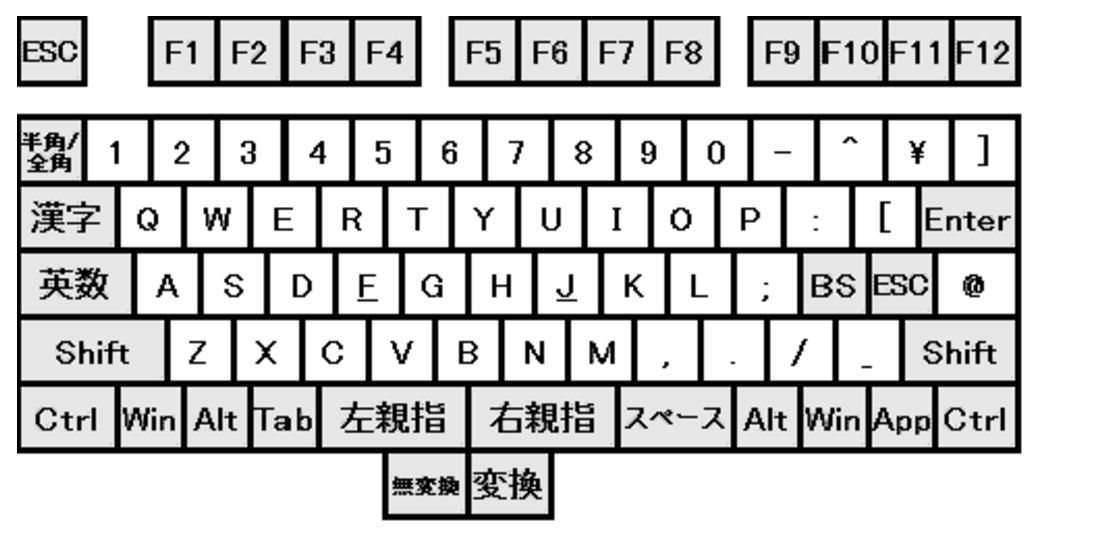
\includegraphics[width=14cm,clip]{res_kouy/oyayubi-shift_keyboard.eps}
 \end{center}
 \caption{�e�w�V�t�g�L�[�{�[�h}
 \label{oyayubi-shift_keyboard}
\end{figure*}

�ł��܂��e�w�V�t�g��������߂�K�v�͂���܂���B���݂ł͕��ʂ̃L�[�{�[�h���g���Đe�w�V�t�g�����邱�Ƃ��ł���̂ł��B�z��G�~�����[�^���g���΁A�L�[�{�[�h�̍ʼn��i�ɂ���\key{���ϊ�}�A\key{�X�y�[�X}�A\key{�ϊ�}�̂ǂꂩ2�L�[��e�w�L�[�Ƃ��āA���������e�w�V�t�g�L�[�{�[�h�̂悤�Ɏg�����Ƃ��ł��܂��B�Ⴆ�΁A\key{�X�y�[�X}��\key{���e�w}�A\key{�ϊ�}��\key{�E�e�w}�ł��邩�̂悤�Ɉ����āA�e�w�V�t�g���������邱�Ƃ��ł���̂ł��B

�u�e�w�L�[�ɂ����L�[�����X�̃L�[�̋@�\���g�������ꍇ�͂ǂ�����΂����̂��H�v�Ƃ����^�₪�킫�܂����A�G�~�����[�^�̕��Łu�����L�[�Ɠ����ɉ������ꍇ�̓V�t�g�L�[�Ƃ��āA�����L�[���������ɗ������ꍇ�͂��Ƃ��Ƃ̃L�[�Ƃ��āv�������Ă���܂��B�Ⴆ�΁A\key{�X�y�[�X}��\key{���e�w}�ɂ����ꍇ�ł��A\key{�X�y�[�X}��P�ɉ����ė������ꍇ�́A���ʂ�\key{�X�y�[�X}�����������̂Ƃ��Ĉ����Ă���܂��i���̂悤�ɂ��Ȃ��Őe�w�V�t�g��p�̃L�[�Ƃ��邱�Ƃ��ł��܂��j�B

�ǂ̃L�[��e�w�L�[�ɂ��邩�́A�����‚��̕��@������܂��B�s\key{�X�y�[�X}��\key{���e�w}�A\key{�ϊ�}��\key{�E�e�w}�t���s\key{���ϊ�}��\key{���e�w}�A\key{�ϊ�}��\key{�E�e�w}�t�ɂ���̂���ʓI�ł��B�|�C���g�ƂȂ�̂͐e�w�L�[�̈ʒu�ł��B�z�[���|�W�V�����Ɏw��u�����Ƃ��ɁA�e�w���u�e�w�L�[�v�̏�Ɏ��R�ɒu����̂����z�ł��B
�����L�[�Ɛe�w�L�[�𖳗��Ȃ������Ō��ł��邩�ǂ������d�v�ł��B���ɁA�e�w�L�[�Ɠ����ɉ����Ƃ��ɁA����ł�\key{Z}\key{T}\key{B}�A�E��ł�\key{Y}\key{N}\key{,}\key{.}\key{/}�������Ȃ������Ō��ł��邩���`�F�b�N���܂��傤�B

�܂��A�L�[�{�[�h�ɂ����\key{���ϊ�}�A\key{�X�y�[�X}�A\key{�ϊ�}�̈ʒu��傫���͂��Ȃ�قȂ�܂��B�L�[�{�[�h�͈������̂Ȃ�1000�`3000�~���x���甃���܂��̂ŁA�D�݂̐e�w�L�[�ɂȂ�悤�ȃL�[�{�[�h�ɕς��Ă݂�̂��ǂ��ł��傤�B

����ɁA��_�ȃL�[�{�[�h�����Ă�����܂��B�}\ref{migite_1retu_shift}�����Ă��������B\key{7}\key{Y}\key{H}\key{N}����E�̃L�[���A���ׂĉE��1��ړ����Ă��܂��B�{���Ȃ�\key{J}������ʒu��\key{H}���A\key{K}������ʒu��\key{J}���A�Ƃ����悤�ɉE�肪�S�����镶���L�[�����ׂĉE�Ɉ�񂸂�Ă���̂ł��i����ɁA�����L�[�̉E�[�̃L�[�������ɔz�u����Ă��܂��j�B������u�E����V�t�g�v�ƌĂт܂��B�L�[�J�X�^�}�C�Y�\�t�g���g���΁A���̂悤�ȉ������ȒP�Ɏ����ł��܂��B

�E����V�t�g�̍ő�̖ړI�́A�E��̃z�[���|�W�V�������E�Ɉړ����邱�Ƃł��B�z�[���|�W�V���������炵�Ă��e�w�������L�[�̈ʒu�͂��̂܂܂ł��B����ɂ��z�[���|�W�V�����Ɏw��u�����Ƃ��ɁA�E��e�w�����傤��\key{�ϊ�}�̏�ɗ���A�Ƃ����L�[�{�[�h������������̂ł��B�ꌩ�A�啝�ȕύX�Ȃ̂Ŋ����܂łɎ��Ԃ��|����悤�Ɏv���邩������܂��񂪁A�w�ƕ����L�[�̈ʒu�֌W�͕ς��Ȃ��̂ŁA�����Ɏg����悤�ɂȂ�܂��B�܂��A�E����V�t�g�Ɋ��ꂽ���ƂŒʏ�̃L�[�{�[�h���g���Ă��A���Ȃ��g�����Ƃ��ł��܂��B


\begin{figure*}
 \begin{center}
   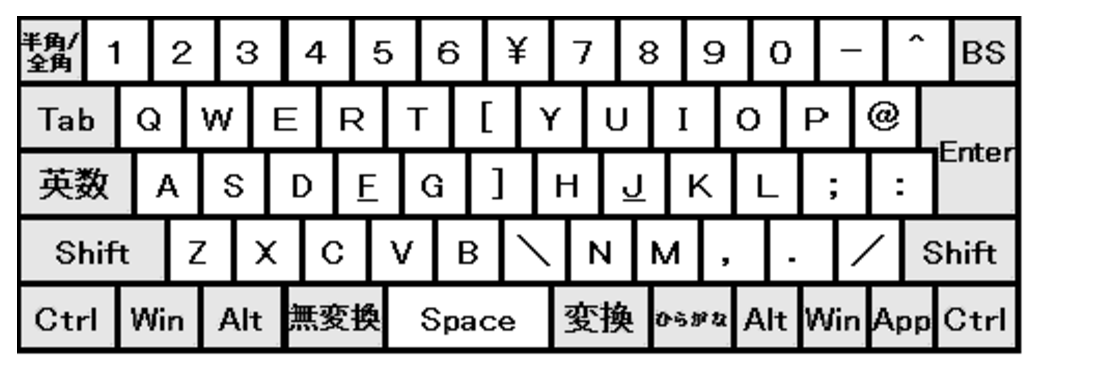
\includegraphics[width=14cm,clip]{res_kouy/migite_1retu_shift.eps}
 \end{center}
 \caption{�E����V�t�g}
 \label{migite_1retu_shift}
\end{figure*}

�������A�e�w�V�t�g�L�[�{�[�h���g�p����΁A�e�w�L�[�̈ʒu�Ƒ傫���͐\����������܂���B�{�i�I�ɐe�w�V�t�g���g�p���邱�Ƃɂ���Ȃ�A�e�w�V�t�g�L�[�{�[�h�̎g�p���I�����ɓ����Ă���ł��傤�B

\subsubsection*{BackSpace�̈ʒu�͑��}

������A�u�e�w�V�t�g�v�Ƃ͒��ڊ֌W�͂���܂��񂪁A�e�w�V�t�g�����͂��₷�����R�������܂��B

�e�w�V�t�g�ł́A�E�菬�w�z�[���|�W�V������1�‰E�̃L�[�A�‚܂�\key{:}�̈ʒu�̃L�[��\key{BackSpace}�����蓖�Ă��Ă��܂��B�ʏ�A\key{BackSpace}�͕����L�[�̉E��̊O��́A���Ȃ艓���ʒu�ɂ���܂��B�������A\key{BackSpace}�͕��͓��͂��s�����ōł��悭�g���L�[�̈�‚ł��B�ǂ�Ȃɏn�����Ă��^�C�v�~�X�𖳂����̂͗e�ՂȂ��Ƃł͂���܂���B�l���Ȃ��當�͂���͂���Ƃ��́A���ܓ��͂����������������ꍇ������܂��B���̂��тɉ�����\key{BackSpace}�������ɍs���Ƃ����̂͑�ςȘJ�͂ł��B\key{BackSpace}���߂��ɔz�u���邱�Ƃ́A�V�z��̎g�p�ɏ���Ƃ����Ȃ����͉��P���ʂ�����܂��B

�܂��A�V�z����K������Ƃ����_���猩�Ă��A\key{BackSpace}�������₷�����Ƃ͏d�v�ł��B�V�z�����K����ۂ́A�ǂ����Ă��^�C�v�~�X���������܂��B\key{BackSpace}�������₷���ʒu�ɂ���΁A�^�C�v�~�X�����Ă������ɏC���ł���̂ŁA�^�C�v�~�X�����ꂸ�ɂǂ�ǂ���͂��邱�Ƃ��ł��܂��B�ǂ�ǂ���͂ł���Α�������邱�Ƃ��ł��A�V�z��̏K���������Ȃ�܂��B

�e�w�V�t�g�ł́A\key{BackSpace}�̔z�u�ꏊ���A\key{:}�Ƃ����z�[���|�W�V��������߂��ʒu�Ɋm�ۂ���Ă��܂��B�e�w�V�t�g���g���ƁA�����I��\key{BackSpace}�������₷���ʒu�ɔz�u����邱�ƂȂ�܂��B����͐e�w�V�t�g�̉B�ꂽ�����b�g�ł��B

�e�w�V�t�g�ȊO�̔z��ł́A\key{BackSpace}�̈ʒu�͍l�����Ă��Ȃ����̂���������܂��B���{����͔z���\key{BackSpace}�̈ʒu���K�肷��Ƃ����̂��ςȘb�ł�����A���R�ƌ����Γ��R�ł��B�������A���܏������ʂ�\key{BackSpace}�̈ʒu�͓��{����͂ɂ����ĂƂĂ���؂ł��B\key{BackSpace}�̈ʒu�����߂��Ă��Ȃ��V�z����g���Ƃ��Ă��\�\�����ƌ����΁A�V�z����g�킸���[�}�����͂₩�ȓ��͂��g���Ƃ��Ă��\�\\key{BackSpace}��ł��₷���ꏊ�ɔz�u���邱�Ƃ��l���ėǂ��Ǝv���܂��B�Ⴆ�΁A�e�w�ɃV�t�g�L�[��z�u���Ȃ��z����g�p����Ȃ�A\key{���ϊ�}��\key{�ϊ�}�͐�D�̌��ƂȂ�܂��B

\subsection{���z��}

���z��́A���w�V�t�g�Ƃ����V�t�g�������g�p����z��ł��B�ʏ�̃V�t�g�L�[�i\key{Shift}�j�͕����L�[�̊O�́A���w�ʼn����ʒu�ɔz�u����Ă��܂��B�e�w�V�t�g�̃V�t�g�L�[�͐e�w�ʼn����ʒu�ɔz�u����Ă��܂����A�g�����L�[�̊O�ɔz�u����Ă���h�Ƃ����_�͒ʏ�̃V�t�g�L�[�Ɠ����ł��B����ɑ΂����w�V�t�g�ł́A��_�ɂ������L�[�̂ǐ^�񒆁A���Ȃ킿���w�̃z�[���|�W�V�����ł���\key{D}��\key{K}�ɃV�t�g�L�[��z�u���܂��B

�}\ref{tuki2-263}�͌��z��̔z��}�ł��B�e�L�[�̉��ɏ�����Ă��镶���͒P�łœ��͂���镶���ł��B����A��ɏ�����Ă��镶����\key{��}�̃L�[�i\key{D}��\key{K}�j�����O�ɉ����Ă����Ƃ��ɓ��͂���镶���ł��B�i�e�w�V�t�g�ƈقȂ�A���z��͓����Ō��ł͂���܂���B���Ƃŏڂ����������܂��j


\begin{figure*}
 \begin{center}
   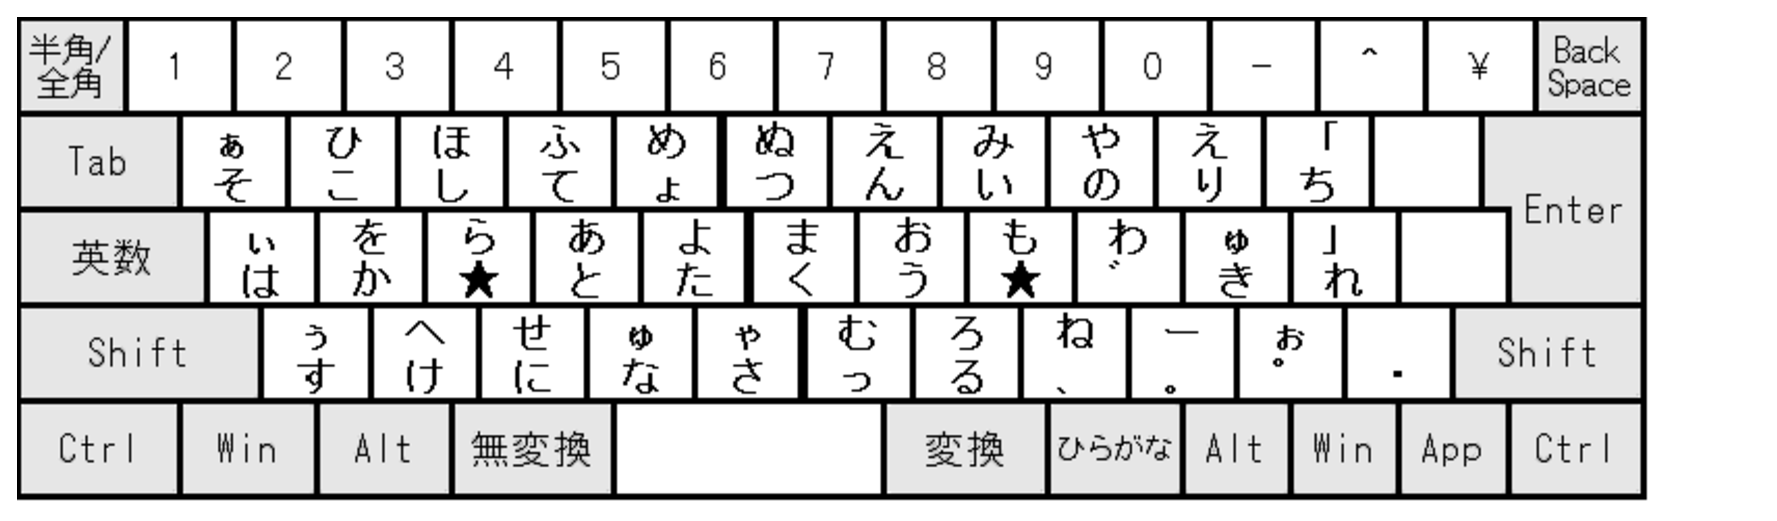
\includegraphics[width=14cm,clip]{res_kouy/tuki2-263.eps}
 \end{center}
 \caption{���z��2-263���z��}}
 \label{tuki2-263}
\end{figure*}

\subsubsection*{���w�V�t�g�̗��_}

���w�̃z�[���|�W�V�����ɃV�t�g��z�u���郁���b�g�́A���ł��傤���H

�܂��A�V�t�g�L�[����ʂȃL�[�ƍl����̂ł͂Ȃ��A�������͂Ɏg��1�‚̃L�[�ƂƂ炦�āA���̎g�p�����ǂꂭ�炢�ɂȂ邩���l���Ă݂܂��B

���{�����͂���ɂ�61��ނ̕�������͂���K�v������܂��i�L���Ȃǂ��܂߂�Ƃ����Ƒ����܂��j�B�܂��A�����̕������L�[�{�[�h�̏㒆���i�̂�����32�L�[���g�p���ē��͂��邱�Ƃɂ��܂��B1�‚̃L�[��1�‚̕�����z�u����̂ł́A�L�[�̐����S�R����܂���B�����ŁA2�‚̃L�[��g�ݍ��킹�ē��͂ł��镶���̎�ނ𑝂₷�u�V�t�g�v�Ƃ����V�X�e�����K�v�ɂȂ�܂��B

���ɁA�o�����̍������32��ނ̕������V�t�g�Ȃ��i�P�Łj�œ��͂��A�c��̕������V�t�g�L�[���g���ē��͂��邱�Ƃɂ��܂��B����Əo�����̒Ⴂ32�`61�ʂ̕����̍��v�o�����͖�16.1\%�ɂȂ�܂��B�‚܂�A���ꂾ���̉񐔃V�t�g�L�[�������K�v������킯�ł��B
�o�������ł����������́u�J�v�i���_�j�Ŗ�10.0\%�A2�ʂ��u���v�Ŗ�5.6\%�A3�ʂ��u���v�Ŗ�5.0\%�Ƒ����܂��B�V�t�g���g�p���镶���́A�����̃g�b�v�N���X�̏o�����̕����Ɣ�ׂĂ��������ŏo�����邱�Ƃ��킩��܂��B

���������āA�V�t�g�L�[����ʂȃL�[�ƍl�����A�u�悭�g���g�����h�͍ł������₷���ʒu�ɔz�u����v�Ƃ����ł��₷���z�������{�I�Ȕ��z�ɗ����čl����ƁA�ق��̂ǂ̕��������A�V�t�g�L�[�����A�ł��ǂ��ʒu�ɔz�u����ׂ����A�Ƃ������ƂɂȂ�܂��B�ł������₷���L�[�Ƃ��ẮA�l�����w�ƒ��w�̃z�[���|�W�V�������l�����܂��B�������A�l�����w�͂��Ƃ��ƒS���L�[�����i�㒆���i��3�i�Ɍ����Ă��j6�L�[�Ƒ������߁A�g�p�������܂�ɂ�����������^����̂ɂ͌����܂���B���������āA���w�̃z�[���|�W�V�����ł���\key{D}��\key{K}���V�t�g�L�[�̖������ʂ����̂ɍœK�ȃL�[�Ƃ������ƂɂȂ�܂��B

\subsubsection*{���z���������̂͒N���H}

���w�V�t�g�Ƃ������͕����́A�Ԕz��Ƃ����z��Œa�����܂����B1999�N�ɕy�~�땶�����l�Ă����z��ŁA�u���v�Ƃ��������ϊ��V�X�e���Ŏg�p���邱�Ƃ�z�肵�č���܂����B���w�V�t�g�����߂č̗p���A�R���s���[�^���g�p�����v�Z�ɂ�蕶���̔z�u�����肵���z��ł��B

�Ƃ���ŁA�VJIS�z��Ƃ����z�񂪂���܂��B1986�N�ɐ��肳�ꂽ�z��ŁA�]����JIS�z��i���ʂ̂��ȓ��͂̂��Ɓj�Ƃ͈قȂ�A�ŏ�i�i�����i�j�͎g�킸�㒆���i��3�i�ɂ��ׂĂ̕������z�u����Ă��܂��B���Z���ȏ���V���l��̃f�[�^���g�p���āA���E���ݑŌ��������A���w�ٌ������Ȃ��Ȃ�悤�ɍ���܂����B���ۂɐVJIS�z�񂪓��ڂ��ꂽ���[�v������������܂������A���y�͐i�܂��A1999�N�Ɂu�g�p���Ԃ��Ȃ����ߔp�~�v����܂����B

�VJIS�z����Ȃ��Ȃ��D�ꂽ�z�񂾂Ǝv���̂ł����A��–��m�Ȍ��_������܂����B����́A�ʏ�̏��w�ʼn����V�t�g�L�[���g�p���邱�Ƃł��i�Z���^�[�V�t�g���l������Ă��܂������A�������Ȃ������悤�ł��j�B�V�t�g�̎g�p���͏]���̂��ȓ��͂��������̂ŁA���w�ŃV�t�g�L�[�������Ə��w�̎g�p�������Ȃ荂���Ȃ��Ă��܂��̂ł��B

�u����Ȃ�VJIS�z��Œ��w�V�t�g���̗p����Ηǂ��̂ł͂Ȃ����H�v�A����Ȕ��z�����܂�܂����B�ǂ��Ő��܂ꂽ���Ƃ����ƁA���{�ő�̓d�q�f���A�Q�����˂�ł��B
2002�N�A�Q�����˂�̃p�\�R����ʔ‚Ɂu�y���[�}��,����,�e�w?�z�VJIS�z��L�[�{�[�h�v�Ƃ����X���b�h�������܂����B�����̘b��͐VJIS�z��̕]����g�p�@�ł������A�������ɑ��̔z��Ƃ̔�r�������悤�ɂȂ�A�Ԕz��̒��w�V�t�g���b��ɏオ��܂����B����ȗ���̒��Łu�w���w�VJIS�z��x�͂ǂ����H�v�ƒ�Ă��郌�X���������܂�܂��B�����Ď��ۂɒ��w�VJIS�z��������҂�����n�߁A����͂��񂾂�Ɛl���𑝂��Ă����A�������҂��獂�]���̃��X���������܂�܂��B

�₪�āA���w�VJIS�z��̈��̂Ƃ��āu���v����Ă���āA���̃X���b�h�̃^�C�g���́u�VJIS�E�� �L�[�{�[�h�z�� 2�Ō��ځv�Ɓu���v�Ƃ������̂����邱�ƂɂȂ�܂����B

�VJIS�z��͒��w�V�t�g�̂��߂ɍ��ꂽ�z��ł͂���܂���̂ŁA���̂܂ܒ��w�V�t�g�����邱�Ƃ͂ł��܂���B�VJIS�z��𒆎w�V�t�g�p�ɉ��ǂ���K�v������܂��B���ɁA�VJIS�z��Œ��w�̃z�[���|�W�V�����ɔz�u����Ă����������ǂ����邩�����ɂȂ�܂��B

�u�VJIS�z��̗ǂ����c�����܂ܒ��w�V�t�g������ɂ͂ǂ��z�u������ǂ����v�B�X���b�h���ł��܂��܂ȋc�_�����킳��A�����̉��LjĂ���Ă���܂����B�����Â��ɁA�ǂ���炱��ł��܂��������悤���Ƃ����z�񂪊������܂��B��������z��2-263���ƌĂт܂��B2-263�Ƃ����̂́A�VJIS�E���z��X���b�h��2�X���ڂ́A263�Ԃ̃��X�Œ�Ă��ꂽ�z��Ƃ����Ӗ��ł��B���̌�����ǂ͐i�߂��܂������A2-263���̈��p�҂͑����A2-263�������z��̍ł��W���I�Ȕz��Ƃ����ʒu�Â��ɂȂ��Ă��܂��B

���z��́A�VJIS�z��ƒ��w�V�t�g�Ƃ����g�ݍ��킹�̖����A�܂����o���Ă��܂��B�����āA���ꂪ���܂ꂽ�̂��C���^�[�l�b�g�̌f���‚ŁA�s���葽���̐l�̋��͂Ŋ��������Ƃ����_���ɂ߂Č��ݓI�ŁA�V�z��̏ے��ƌ����鑶�݂��Ǝv���̂ł��B

\subsubsection*{�G�~�����[�^�Ȃ�Ă���Ȃ��H}

���z��̒��w�V�t�g�́u�O�u�V�t�g�v�Ƃ����V�t�g�����œ��͂��܂��B�e�w�V�t�g�͓����Ō��ł������A���z��͓����Ō��ł͂���܂���B

�O�u�V�t�g�Ƃ����̂́A�u���̃L�[�������O�ɃV�t�g�L�[�������B�V�t�g�L�[�𗣂������ǂ����͖��Ȃ��v�Ƃ����V�t�g�����ł��B�Ⴆ�΁A���z��ŒP��\key{J}�������Ɓu���v�Ɠ��͂���܂����A���\key{D}�������Ă���\key{J}�������Ɓi\key{D}�𗣂������ǂ����͖��Ȃ��j�u���v�Ɠ��͂���܂��B

���̑�����Âɍl���Ă݂�ƁA�L�[�������^�C�~���O�̓��[�}�����͂Ɠ����ł��B���[�}�����͂ł��A�P��\key{A}�������Ɓu���v�Ɠ��͂���A\key{K}�������Ă���\key{A}�������Ɓu���v�Ɠ��͂���܂��B���z�������Ɠ������Ƃ����Ă��܂��B���������āA���z��͍��܂Ŏg���Ă������[�}�����͂ł̃L�[���������o�œ��͂ł���Ƃ��������b�g������܂��B

����ɁA�u���[�}�����͂Ɠ����V�X�e���ł���v�Ƃ������Ƃ���A�ӊO�ȃ����b�g�������܂��B����́uIME�̃��[�}���J�X�^�}�C�Y�Ŏ����ł���v�Ƃ������Ƃł��B���[�}���J�X�^�}�C�Y�Ƃ����̂́A���[�}���̂‚Â��ύX�ł���IME�̋@�\�ł��B�Ⴆ�΁A�ʏ탍�[�}�����͂ł�\key{K}�̎���\key{A}�������Ɓu���v�Ɠ��͂���܂��B����\key{K}��\key{A}�̕�����ύX�ł���̂ł��B���������āA\key{S}�������Ɓu���v�Ɠ��͂����悤�ɐݒ肷�邱�Ƃ��”\�Ȃ킯�ł��i�Ȃ��A�@�\�̖��̂�IME�ɂ���ĈقȂ�܂��B�wMicrosoft IME�x�ł́u���[�}���ݒ�v�A�wATOK�x�ł́u���[�}���J�X�^�}�C�Y�v�A�wGoogle ���{����́x�ł́u���[�}���e�[�u���v�Ƃ������̂ł��j�B

�V�z����g���ꍇ�̕s���_�̈�‚ɁA�u�����ł��邩�ǂ����v�Ƃ������̂�����܂��B�z��G�~�����[�^�Ŏ�������ꍇ�A���܎g���Ă���p�\�R���ŃG�~�����[�^�����Ғʂ�ɓ����Ȃ��”\��������܂��B�����̃p�\�R���ł͓����Ă��A�ʂ̃p�\�R���ł͓����Ȃ���������܂���B���͓����Ă����������Ȃ��Ȃ�Ƃ����s�������S�ɕ��@���邱�Ƃ͂ł��܂���B

���̓_�A���z��͂��Ȃ���S�ł��B�Ȃ��Ȃ�AIME�̃��[�}���J�X�^�}�C�Y�Ŏ������邱�Ƃ��ł��邩��ł��B���z��̃V�t�g�̃V�X�e���̓��[�}�����͂Ɠ����ł��̂ŁA���[�}���J�X�^�}�C�Y���g����IME�̋@�\�݂̂Ō��z��������ł��܂��B�G�~�����[�^���g���K�v������܂��񂩂�A�u�����ł��Ȃ��v�Ƃ����S�z�͂��Ȃ菭�Ȃ��Ȃ�܂��B

�������AIME�ɂ���Ă̓��[�}���J�X�^�}�C�Y�ɐ���������ꍇ������̂ŁA���z��̂��ׂĂ��������邱�Ƃ͂ł��Ȃ����Ƃ�����܂��B���̏ꍇ�AIME�p�ɏ����A�����W���Ď������邱�ƂɂȂ�܂��B�wGoogle ���{����́x�̃��[�}���J�X�^�}�C�Y�͔��ɋ��͂ł��̂ŁA�قڐ��������������邱�Ƃ��ł��܂��B

�܂��A�G�~�����[�^���g���ꍇ�ł����Ă��A�����Ō��Ȃǂ̕��G�ȑ��삪�Ȃ��̂ŁA�G�~�����[�^�̑I�����������A��������r�I�ȒP�ł��B�u���܂��܂Ȋ‹��ŐV�z����g�p�������v�u����G�~�����[�^�͎g�����Ȃ��Ȃ��v�Ǝv���l�ɂ��������߂ł��B

\subsection{AZIK}

���܂ŏЉ���u�e�w�V�t�g�v�Ɓu���z��v�́A���܂܂Ŏg���Ă������[�}�����͂Ƃ͂܂������ʂɁA�ꂩ�炩�Ȃ�z�u���������z��ł����B����ɑ΂��Ă��ꂩ��Љ��uAZIK�v�́A���܂Ŏg���Ă������[�}�����͂͂��̂܂ܐ������āA���̒��œ��͕��@�����P���悤�Ƃ����z��ł��B

\subsubsection*{���[�}�����͊g���z��Ƃ́H}

AZIK�́A���[�}�����͂��g�����āA���[�}�����͂ł͓��͂��ɂ������������P����z��ł��B

�Ⴆ�΁A���[�}�����͂Łu����v�Ɠ��͂���ꍇ��\key{S}\key{Y}\key{A}�Ɠ��͂��܂��B����͓�����O�̂��Ƃ̂悤�ł����A������\ruby{�X��}{�悤����}�̓��͂�3�Ō�������Ƃ����̂́A�����I�ł͂���܂���B�u����v��\key{J}\key{A}��2�Ō��œ��͂ł��邱�Ƃ��l����Ε�����悤�ɁA�X�����{����2�Ō��œ��͂ł��ėǂ��̂ł��B������AZIK�ł́A\key{X}�ł���s����͂ł��邱�Ƃɂ��܂��B�Ⴆ�΁A�u����v�Ɠ��͂���ꍇ��\key{X}\key{A}��2�Ō��œ��͂��܂��B����s�̝X���͂��Ȃ�o�����������̂ŁA���ꂾ���ł����\�ȓ��͉��P���ʂ�����܂��B

�ق��ɂ��AAZIK�ł͎��̂悤�Ȋg�����͂��g�p�ł��܂��B
\begin{itemize}
 \item \key{;}�i\key{L}��1�‰E�̃L�[�j�Łu���v����͂���B���[�}�����͂ł́u���v�̓��͕��@�́A�ꍇ�ɂ���Ďg���L�[���قȂ�ȂǕϑ��I�ł��B���̓��͕��@���g�����ƂŁA��ɕ�����₷�����͂��邱�Ƃ��ł��܂��B
 \item \key{C}�ł���s�̝X������͂���B�i��F\key{C}\key{A}�Łu����v�Ɠ��͂���j
 \item \key{Q}�Łu��v����͂���B���[�}�����͂ł́u��v�̓��͕��@�́A\key{N}�����œ��͂ł�����A\key{N}\key{N}�ȂǂƓ��͂��Ȃ���΂Ȃ�Ȃ��ꍇ���������肵�āA�ϑ��I�ł��B���̓��͕��@���g�����Ƃŏ��1�Ō��œ��͂��邱�Ƃ��ł��܂��B
 \item \key{:}�i\key{L}��2�‰E�̃L�[�j�Łu�[�v����͂���B�u�[�v�̓��[�}�����͂ŗB��ŏ�i���g�������ŁA���͂��Â炢�����ł��B������z�[���i�œ��͂ł���悤�ɂ��܂��B
\end{itemize}
AZIK�ł͂��̂悤�Ȋg�����͂�ςݏd�˂邱�ƂŁA���[�}�����͂����ł��₷���Ȃ�悤���P���Ă��܂��B

\subsubsection*{���[�}�����͂͂��̂܂܎g����}

AZIK�̊g�����͂̏d�v�ȓ_�́A���̂悤�ȉ��ǂ��d�˂Ă��A���Ƃ��Ƃ̃��[�}�����͂͂قڂ��̂܂܎g����Ƃ������Ƃł��B

�ŏ��ɁA\key{X}�ł���s�̝X������͂ł���Ə����܂����B�������A����́u����s�̝X������͂���Ƃ��͕K��\key{X}���g���v�Ƃ����Ӗ��ł͂���܂���B����\key{X}\key{A}�ł���s�̝X������͂ł��邱�Ƃ�Y��Ă��܂�����A�ʏ�ʂ�\key{S}\key{Y}\key{A}�Ɠ��͂��邱�Ƃ��ł��܂��B�܂��A\key{X}�Ƃ����L�[�́A���[�}�����͂ł͂قƂ�ǎg�p���܂���i�������̂��Ȃ̓��͂�\key{L}�ł��ł��܂��̂�\key{X}���g���K�v�͂���܂���j�B\key{X}�ł���s����͂ł��邱�Ƃɂ��Ă��A���Ƃ��Ƃ̃��[�}�����͂͂قڂ��̂܂܎g�p���邱�Ƃ��ł��܂��B

�ق���AZIK�̊g�����͂����Ă��A�u���v�̓��͂Ɏg��\key{;}�A�u��v�̓��͂Ɏg��\key{Q}�A�u�[�v�̓��͂Ɏg��\key{:}�ȂǁA���Ƃ��Ƃ̃��[�}�����͂ł͂قƂ�ǎg��Ȃ��L�[�΂���ł��B

���̂悤�ɁAAZIK�̊g�����͂́A�{���̃��[�}�����͂ł͎g��Ȃ��L�[��A�L�[�̑g�ݍ��킹���g���čs���܂��B���������āAAZIK������������Ԃł��AAZIK�̊g�����͂��܂������g�킸�A���[�}�����͂̂悤�ɓ��͂��邱�Ƃ��”\�ł��B���[�}�����͂��u�ύX�v���Ďg���₷������̂ł͂Ȃ��A�{���̃��[�}�����͂��u�g���v���邱�Ƃɂ���Ďg���₷������B���ꂪAZIK�̍ő�̓����ł��B

\subsubsection*{AZIK�̊o���₷��}

AZIK�̉��ǂ��u�g���v�ł��邱�Ƃ̃����b�g�́A���[�}�����͂��g�����܂܁A���͕��@�����P�ł��邱�Ƃł��B

�V�z����o���邱�Ƃœ��͌��������P���邱�Ƃ��ł��܂����A���͐V�z����o����܂ł̊��Ԃ��ǂ����邩�ł��B�ǂ�ȊȒP�Ȕz��ł��A�V�z����K������ɂ͂�����x�̗��K���Ԃ��K�v�ł��B�K���܂ł͕��͓��͂��܂Ƃ��ɂł��܂���B�V�z����g�������Ǝv���Ă��A���̊��Ԃ̂‚炳���v���Ă�����߂Ă��܂����������ł��傤�B

AZIK�Ȃ炻�̐S�z�͂���܂���BAZIK�Ȃ�A���܂Ŏg���Ă������[�}�����͂͂قڂ��̂܂܎g���܂��B���������āAAZIK�����S�ɏK�����Ă��Ȃ��i�K�ł��A�����Ɏ��ۂ̕��͓��͂Ŏg�p���邱�Ƃ��ł��܂��B�ł���͈͂Ŋg�����͂��g���A�Y��Ă��܂����烍�[�}�����͂̕��@�œ��͂���΂悢�̂ł��B��������Ďg���Ă��������Ɋ���Ċo���邱�Ƃ��ł��܂��B

�����āAAZIK�͊��S�Ƀ}�X�^�[����K�v���炠��܂���BAZIK�̊g�����͂́A��ɏЉ���ȊO�ɂ����܂��܂Ȃ��̂��p�ӂ���Ă��܂��B���ɂ͂��Ȃ荂�x�Ȋg��������܂��B�������AAZIK���g�p����̂ɂ�����g�����Ȃ��Ȃ���΂Ȃ�Ȃ��Ƃ������Ƃ͂���܂���B�u����s��\key{X}�œ��͂���v�u�u���v��\key{;}�œ��͂���v�Ƃ����ȒP�Ȋg�����͂������g���Ƃ����g�p���@�ł��ǂ��̂ł��B�ȒP�Ȋg�����܂��g���Ă݂āA����Ŋo�����鎩�M���‚����玟�̊g�����͂ɐi�ނ��Ƃ��ł��܂����A����ŏ\�����Ǝv���΂����܂ł̒i�K�Ŏg�������邱�Ƃ��ł��܂��B�����Ă��‚��]�T���ł�����A���߂Ď��̊g�����͂Ƀ`�������W����Ƃ������Ƃ��ł���̂ł��B

\subsection{Dvorak���[�}��}


\begin{figure*}
 \begin{center}
   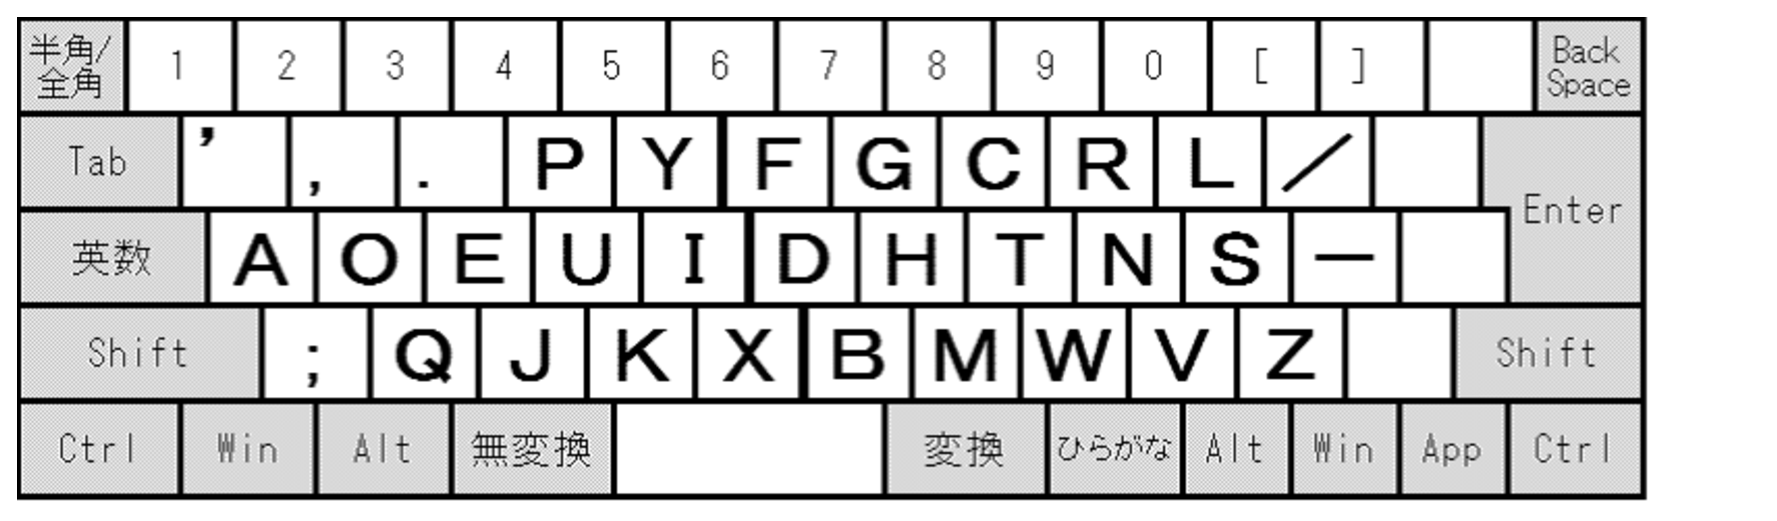
\includegraphics[width=14cm,clip]{res_kouy/Dvorak.eps}
 \end{center}
 \caption{Dvorak�z��}}
 \label{Dvorak}
\end{figure*}

\subsubsection*{�p����͂����P���悤}

����܂ŏЉ���V�z��́A���ׂāg���{��ł́h���͂����P���悤�Ƃ�����̂ł����B����A�p��ł����͕��@�����P���悤�Ƃ����z�񂪑��݂��܂��B��ʓI�ɑ����g���Ă���A���t�@�x�b�g�̔z��̂��Ƃ��A�L�[�{�[�h�̏�i�̍�����6����������āuQwerty�z��v�ƌĂт܂��BQwerty�z��ɑ���z��Ƃ��ėL���Ȃ̂��uDvorak�z��v�ł��B

Dvorak�z��̐��藧���͌Â��A1932�N�ɃA�����J�Ő��܂�܂����B�l�Ď҂̃I�[�K�X�g�E�h���H���b�N���O�������Dvorak�z��ƌĂ΂�Ă��܂��B�p���ł̃A���t�@�x�b�g�̏o������L�[�̑ł��₷�����l�����Ċe�����̔z�u�����߂��Ă��܂��B�ꉹ�����ׂč���̃z�[���i�ɔz�u����Ă���̂������BQwerty�z��ɔ�ׂČ��ݑŌ����������A�w�̈ړ��������Z���Ȃ�܂��B�^�C�s���O���x����K���̌���A\ruby{�F�≊}{���񂵂傤����}�Ȃǂ̖h�~�Ɍ��ʂ�����ƌ����Ă��܂��B

���́ADvorak�z��̓��[�}�����͂�����ꍇ���D�ꂽ�z��ł��B�Ƃ����̂́ADvorak�z��̓��[�}�����͂̕ꉹ�ł���\key{A}\key{I}\key{U}\key{E}\key{O}������̃z�[���i�ɕ��ׂĔz�u����Ă��邩��ł��BQWERTY�z��̃��[�}�����͂̌��_�́A�ł��悭�g���L�[�ł���ꉹ�L�[���A�ł��ł��₷���ꏊ�ɂ͔z�u����Ă��Ȃ����Ƃł����B\key{A}�����w�̃z�[���|�W�V�����ɂ��邾���ŁA�ق���4�L�[�͂��ׂăz�[���i����O�ꂽ�ꏊ�ɂ���܂��BDvorak�z��Ȃ�ꉹ�����ׂăz�[���i�ɂ���܂��B���������ĕꉹ����͂���Ƃ��Ƀz�[���|�W�V��������w������ɂ����A�����I�ɓ��͂��邱�Ƃ��ł��܂��B

���{��̓��͂ƂƂ��ɉp��̓��͂����P�������Ƃ������́ADvorak�z����o���ė�����C�ɂ���ʼn�������Ƃ����̂��ǂ��Ǝv���܂��B

\subsubsection*{Dvorak���[�}�����g�����悤}

�������A���R�Ȃ���Dvorak�����[�}�����͗p�ɍ��ꂽ�z��ł͂���܂���̂ŁADvorak�z��ł��̂܂܃��[�}�����͂����悤�Ƃ���ƁA�����‚��C�ɂȂ�_���o�Ă��܂��B
��\�I�Ȃ̂��A\key{K}���ꉹ�Ɠ������葤�ɂ��邱�Ƃł��B���̂��߁A���s�̂��Ȃ���͂��邽�тɍ���𑱂��Ďg�����ƂɂȂ�܂��B���ɁA�u���v�Ɓu���v����͂���Ƃ��ɍ���̐l�����w�𑱂��Ďg�����ƂɂȂ�̂����ł��B

���̖��̉�����Ƃ��ėL���Ȃ̂́A���s�̓��͂�\key{K}�̑����\key{C}�łł��邱�Ƃɂ���Ƃ������@�ł��B���o�I�ɂ��ACA�Łu���v�Ɠǂ߂܂����ACA�ECU�ECO�Łu���E���E���v�Ɠ��͂ł���IME�������ł��B�����Ζ��Ȃ����͂ł���ł��傤�B

����ɉ��Ǔ_���g�債�āAAZIK�̂悤�Ȋg�����[�}�����͂�Dvorak�z��ɂقǂ������z�������܂��B�wDvorakJP�x�͔�r�I���₩�ȉ��ǁB����Dvorak�z�񂩂�ύX�_�����Ȃ��A�Ȃ��݂₷���Ǝv���܂��B�wACT�x�͓��ݍ��񂾉��ǁB�uAZIK�v�Ɠ����悤�ɊȒP�Ȋg�����獂�x�Ȋg���܂ŕ��L�������A�ł��ɂ����^�w���ł������Ȃ�����_�ȉ��ǂ��{���Ă��܂��B

������Dvorak�g���z��́A���ɂ��Ă���Dvorak�z�񎩑̂����[�}�����͂ɓK���Ă���̂ŁA�p��z��𗣂�āA�P�ɓ��{����͔z��Ƃ��Č��Ă����Ȃ苭�͂ł��B��������Dvorak�z����o����̂Ȃ�A���{����͂̕��͍ŏ�����Dvorak�g���z����o����Ƃ����̂��ǂ��ł��傤�B

\subsection{�����Ȃ��}


\begin{figure*}
 \begin{center}
   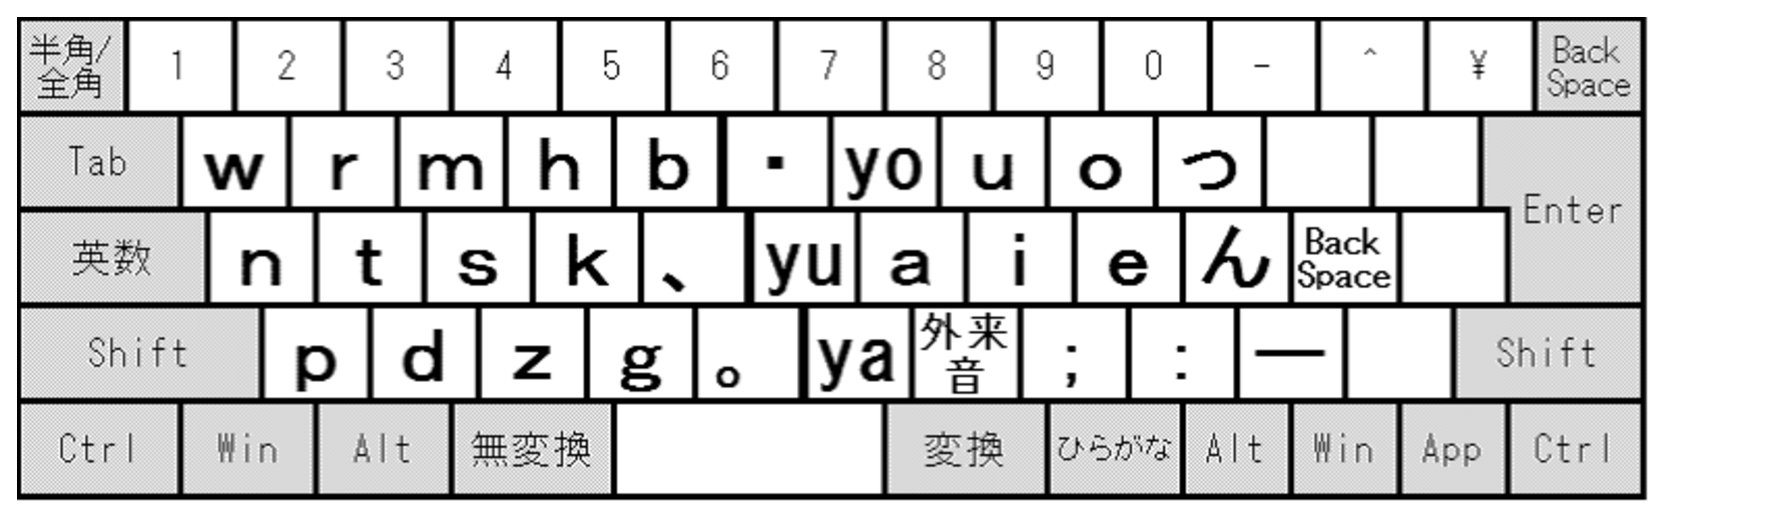
\includegraphics[width=14cm,clip]{res_kouy/keinarabe.eps}
 \end{center}
 \caption{�����Ȃ�הz��}}
 \label{keinarabe}
\end{figure*}

\subsubsection*{�܏\�����s�i�n�z��}

�����Ȃ�ׂ́A�o���₷���ɏd�_���������s�i�n�z��ł��B�s�i�n�Ƃ����̂́A1�‚̕�������{�I�Ɏq���ƕꉹ��2�Ō��œ��͂���z��̂��Ƃł��B���Ȃ̌܏\���\�𗘗p���āA�q���ƕꉹ��g�ݍ��킹�邱�Ƃ�1�‚̂��Ȃ���͂��܂��B���[�}�����͂��s�i�n�z��̈��ł��B

�����āA�����Ȃ�ׂł͎q���ƕꉹ�����E�ɂ͂����蕪����Ĕz�u����Ă��܂��i�}\ref{keinarabe}�j�B���肪�q���L�[�S���A�E��ɕꉹ�L�[�S���ł��B

����ɁA���̃L�[�̕��ѕ������Ȃ�K���I�ł��B�q������͂���L�[�͍���l�����w�̃z�[���|�W�V�����ł���\key{F}���N�_�Ƃ��āA�������獶�ɂ��s�A���s�A���s�A�ȍs�̏��ԁB��i�Ɉڂ���\key{R}����͍s�A�܍s�A��s�A��s�̏��ԂƂȂ��Ă��܂��B����͂��Ȃ��݂̌܏\�����Ɠ������Ԃł��i�Ȃ��A�����Ȃ�ׂł͂�s�̎q���L�[�͂���܂���B���Ƃŏڂ����������܂��j�B����ɑ�������͂���L�[���A���s�A���s�A���s�̃L�[�́A���̐����̃L�[�̂������ɔz�u����Ă��܂��B�ꉹ���A���ϑ��I�ł͂���܂����A�E��̃z�[���|�W�V�����ł���\key{J}���N�_�Ƃ��Ă������������ŕ��ׂ��Ă��܂��B

���̂悤�ɁA�����Ȃ�ׂł͂Ȃ��ݐ[���܏\���̏��Ԃ𗘗p���Ċo������悤�ɍ���Ă��܂��B����Ȃ炷���ɂł��o���邱�Ƃ��ł���ł��傤�B

\subsubsection*{���E���ݑŌ��ƃA���y�W�I�̈З�}

�u�m���ɂق��̔z����o���₷�����ł͂��邯�ǁA�s�i�n�Ƃ������Ƃ͊�{�I��1�‚̂��Ȃ̓��͂�2�Ō�������B����ł͏K�����Ă��\���ȓ��͉��P���ʂ͓����Ȃ��̂ł́H�v�Ǝv���������邩������܂���B�m���ɁA�����Ȃ�ׂ̑Ō����́A���[�}�����͂��͏��Ȃ����̂́A1�Ō���1�������͂ł��邩�Ȍn�̔z��Ɣ�ׂ�Ƃ��Ȃ葽���Ȃ�܂��B�Ō���������Ȃ��̂ł͉��P���ʂ��債�����Ƃ͂Ȃ����낤�A�ƍ����������邩������܂���B�������A�����Ȃ�ׂ́A���͌������P���ʂ������ĕ��邱�Ƃ͂ł��Ȃ��̂ł��B

�����Ȃ�ׂ����͂��₷�����̗��R�́A��{�I�ɍ��E���ݑŌ��œ��͂ł��邱�Ƃł��B
���E���ݑŌ��Ƃ����̂́A����ŃL�[��ł����玟�͉E��A�E��ŃL�[��ł����玟�͍���Ƃ����悤�ɁA���E�̎�����݂Ɏg���đŌ����邱�Ƃł��B����͓��͂��₷�����͕��@�ł��B�Ȃ��Ȃ�A����̎�ŃL�[��ł��Ă���ԂɁA��������̎�̓L�[���������������邱�Ƃ��ł��邩��ł��B

�����Ȃ�ׂł͎q��������ŁA�ꉹ���E��œ��͂��܂��B�s�i�n�̓��͕��@�ł͊�{�I�Ɏq���ƕꉹ�����݂ɏo�Ă��܂��̂ŁA�K�R�I�ɍ��E���ݑŌ��œ��͂ł���̂ł��B

�������A���E���ݑŌ��ł͓��͂ł��Ȃ�����������܂��B�Ⴆ�΁A�A�ꉹ�̕����ł��B�A�ꉹ�Ƃ����̂́A���[�}���ŕꉹ���A�����ďo�����镔���̂��Ƃł��B�Ⴆ�΁A�u�����v�Ƃ�����������͂���Ƃ���\key{K}\key{A}\key{I}�Ɠ��͂��܂��B�ꉹ��A��I���A�����Ă��܂�����A���̕����͘A�ꉹ�Ƃ������ƂɂȂ�܂��B�����Ȃ�ׂ̕ꉹ�͂��ׂĉE��œ��͂��܂�����A�A�ꉹ�̕����͕K�R�I�ɓ�����𑱂��Ďg�����ƂɂȂ�܂��B

�������A�ނ��낱�̘A�ꉹ�������A�����Ȃ�ׂ̓��͂��₷���̐^�����Ƃ����镔���ł��B���̔閧�́A�A�ꉹ�̕΂�ƁA�A�ꉹ���A���y�W�I�œ��͂ł��邱�Ƃł��B

�A�ꉹ�̏o�����́A���Ȃ̏o�����Ɠ����悤�ɂɑ傫�ȕ΂肪����܂��B�ꉹ��5��ނł�����A�A�ꉹ�͑S����25��ނ���܂��B���̂����o�����̍���ai�Aei�Aou��3��ނ̘A�ꉹ�őS�̖̂�55.3\%���߂܂��B����3��ނ̘A�ꉹ�����ɏo���Ă݂�ƁA�����g�����ł��邱�Ƃ���������Ǝv���܂��B���Ɋ����̉��ǂ݂ő����g���܂��B

�����Ȃ�ׂł́A���̏o�����̍���3�‚̘A�ꉹ���A���y�W�I�œ��͂ł���悤�ɂ��Ă���܂��B�A���y�W�I�Ƃ����̂́A�u�Е��̎�ő����ăL�[�������ꍇ�ɁA���ɉ����₷���A�ځv�̂��Ƃł��B�Ⴆ��\key{K}��\key{J}�ƑŌ�����ꍇ���A���y�W�I�ł��B���ۂɃL�[�������Ă݂�ƁA����2�L�[��Ō�����ꍇ�͑����y�ɑŌ��ł��邱�Ƃ���������Ǝv���܂��B�����Ȃ�ׂł́A�A�ꉹai��\key{J}��\key{K}�Aei��\key{L}��\key{K}�Aou��\key{O}��\key{I}�ƁA���ׂăA���y�W�I�œ��͂ł���悤�ɔz�u���Ă���܂��B�����Ȃ�ׂ̕ꉹ�́A�q���ɔ�ׂ�Ƃ��ϑ��I�ȏ��Ԃŕ���ł��܂����A����͘A�ꉹ���A���y�W�I�őłĂ�悤�ɂ��邽�߂ł��B

��{�͍��E���ݑŌ��A�o�����̍����A�ꉹ�̓A���y�W�I�œ��́B����2�‚̍H�v�ɂ��A�����Ȃ�ׂ͊o���₷���܏\�����z��ł���Ȃ���A�������͉��P���ʂ��������Ă��܂��B

\subsubsection*{����̕ꉹ���Ƃ́H}

�����ЂƂA�����Ȃ�ׂ̑傫�ȓ���������܂��B����́A�u����v��ꉹ�����Ĉ����Ă��邱�Ƃł��B

�ʏ�̃��[�}�����͂ł́A�ꉹ�́uaiueo�v��5��ނł��B�ua�v�͒P�łŁu���v����͂��܂��B�q���uk�v�ƕꉹ�ua�v�̑g�ݍ��킹�Łu���v����͂��܂��B�u����v��ꉹ������Ƃ����̂́A�uya�Ayu�Ayo�v���ua�Ai�Au�Ae�Ao�v�Ɠ��������ɂ���Ƃ������Ƃł��B���������āA�uya�Ayu�Ayo�v��P�łœ��͂ł���L�[�����݂��܂��B�����Ȃ�הz��}�i�}5-6�j��\key{N}\key{H}\key{U}�̃L�[�A�����珇�ԂɁuya�v�uyu�v�uyo�v�ƕ���ł��镔��������ł��B�����̃L�[��P�łʼn����ƁA�u����v�����͂���܂��B����A�q���L�[����������Ɂuya�Ayu�Ayo�v�������ƁA�X������͂��܂��B�Ⴆ�΁A�uk�v�̃L�[�������Ă���uya�v�̃L�[�������Ɓu����v����͂��܂��B�X���Ƃ����̂́A�q���Ƃ�s�̑g�ݍ��킹�ł��ׂĕ\�����邱�Ƃ��ł���̂ł��B

�}\ref{keinarabe_50on}�͂����ꉹ���������܏\���\�ł��B�����ꉹ��������Ƃ����Ɗ�قɎv���邩������܂��񂪁A�\�����ԂȂ����߂���ŝX�����K���I�Ɏ�荞�߂�̂ŁA�ނ���ʏ�̌܏\���\��蕪����₷���܂Ƃ܂��Ă���Ǝv���܂��B


\begin{figure*}
 \begin{center}
   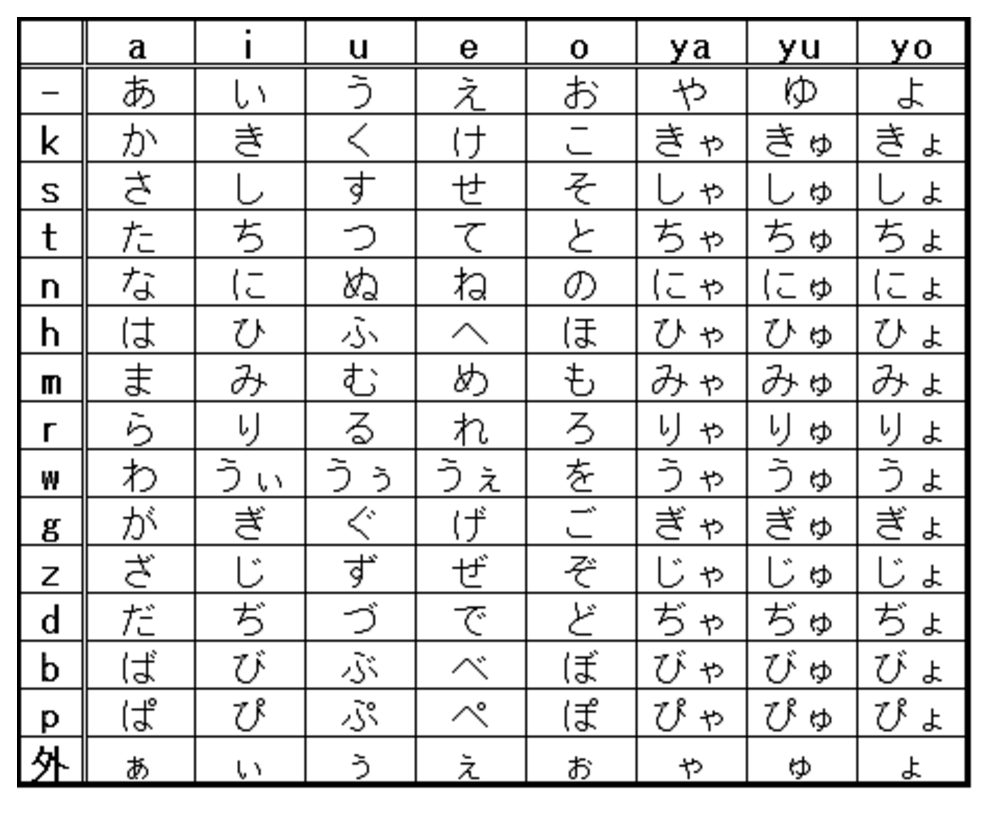
\includegraphics[width=14cm,clip]{res_kouy/keinarabe_50on.eps}
 \end{center}
 \caption{�����ꉹ���������܏\���\}
 \label{keinarabe_50on}
\end{figure*}

�����ꉹ�����郁���b�g��2�‚���܂��A�܂��A�X�������ׂ�2�Ō��œ��͂ł��邱�Ƃł��B�ʏ�̃��[�}�����͂ł͝X���̓��͂͑�����3�Ō��ł��̂ŁA���̕��Ō��������炷���Ƃ��ł��܂��B�ʏ�̃��[�}�����͂ł��A����s�̝X��������2�Ō��œ��͂ł���̂ŁA����s�����͓��͂��₷���Ɗ������Ă�����������Ǝv���܂��B���ꂪ���ׂĂ̝X���Ɋg�傳���̂͑傫�ȃ����b�g�ł��B

������‚́A��s�̘A�ꉹ�̓��͂����₷�����Ƃł��B��قǕp�o����A�ꉹ��ai�Aei�Aou��3�‹����܂����B�������A���͂����ꉹ�������邱�Ƃɂ���ƁAyou�i�傤�j�Ƃ����A�ꉹ�����ɂ悭�o������A�ꉹ�ƂȂ�܂��B�u�傤�v�Ƃ��������̘A�Ȃ�́A2�����̘A�Ȃ�̒��ł͒f�g�c�ł��B�����Ȃ�ׂł́A���̘A�ꉹyou��\key{U}��\key{I}�̃A���y�W�I�œ��͂ł���悤�ɂȂ��Ă��܂��B�u����v���i�ォ��ł͂Ȃ��j�����珇�Ԃɕ���ł���̂́A\key{yo}��\key{u}���A���y�W�I�œ��͂ł���悤�ɂ��邽�߂ł��B

�ʏ�̘A�ꉹ3��ɉ����āA�X���̘A�ꉹyou���A���y�W�I�œ��͂ł��邱�Ƃɂ��A�����Ȃ�ׂ͍s�i�n�̓��͕��@�ł���Ȃ���A�Ō������ӎ������Ȃ��X�s�[�h���̂�����͂����邱�Ƃ��ł���̂ł��B


\clearpage
\articlepart{�������̂��߂̔z��K��}{tomoemon}

\section{�͂��߂�}

�u��葬�����͂ł���悤�ɂȂ肽���v�Ƃ����̂͋��Z�^�C�s���O�Ɏ��g�ސl�Ȃ�N�����v�����Ƃł��B�����ł‚��߂̕��@�_����K�@�ɂ‚��Ă͖{���̑��̋L���ɂ��ڂ��Ă��܂����A���̋L���ł́u�ŏ��Ɋo�����L�[�{�[�h�z��Ƃ͕ʂ̔z��v���K�����č����ȃ^�C�s���O��ڎw�����@�ɂ‚��ďЉ�Ȃ���A���̕��@�̗ǂ��_�A�����_���l���Ă����܂��B

�����ł����u�ŏ��Ɋo�����L�[�{�[�h�z��Ƃ͕ʂ̔z��v�Ƃ́A�Ⴆ�΃��[�}�����͂��ŏ��Ɋo�����l�ɂƂ��Ă̂��ȓ��͂�A���ȓ��͂��ŏ��Ɋo�����l�ɂƂ��Ẵ��[�}�����͂����Ă͂܂�܂��B������񂱂�ȊO�ɂ��AQwerty�z�񂩂�Dvorak�z��ɏ�芷����A�e�w�V�t�g�z��ɏ�芷����Ƃ������l�X�ȏꍇ���l�����܂��B�ǂ̂悤�ȃp�^�[���ɂ���A����̔z��ɉ��炩�̌��E�������āA����ȊO�̔z��ɉ”\�����������Ƃ��ɏ�芷���邱�Ƃ������Ǝv���܂��B�����ł͓��ɓ��͑��x�̌��E�A�”\���Ƃ����ϓ_�ł��̕��@�̗L�����ɂ‚��čl���Ă����܂��B

\section{�p��̊m�F}

\subsection{�L�[�{�[�h�z��}

�u�L�[�{�[�h�z��i���邢�͒P�ɔz��j�v�Ƃ������t�̈Ӗ��ō������邱�Ƃ�����̂Ő�ɐ������Ă����܂��B��ʓI�ɃL�[�{�[�h�z��Ƃ����ƃL�[�{�[�h�Ɉ󎚂���Ă���\key{Q}\key{W}\key{E}\key{R}\key{T}\key{Y}�Ƃ������т̂��Ƃ��C���[�W����Ǝv���܂����A��̂���Ŗ�肠��܂���B�Ⴆ�ΐ}\ref{qwerty}��Qwerty�z��ƌĂ΂����̂Ō��ݍL�����y���Ă�����̂ł��B


\begin{figure*}
 \begin{center}
   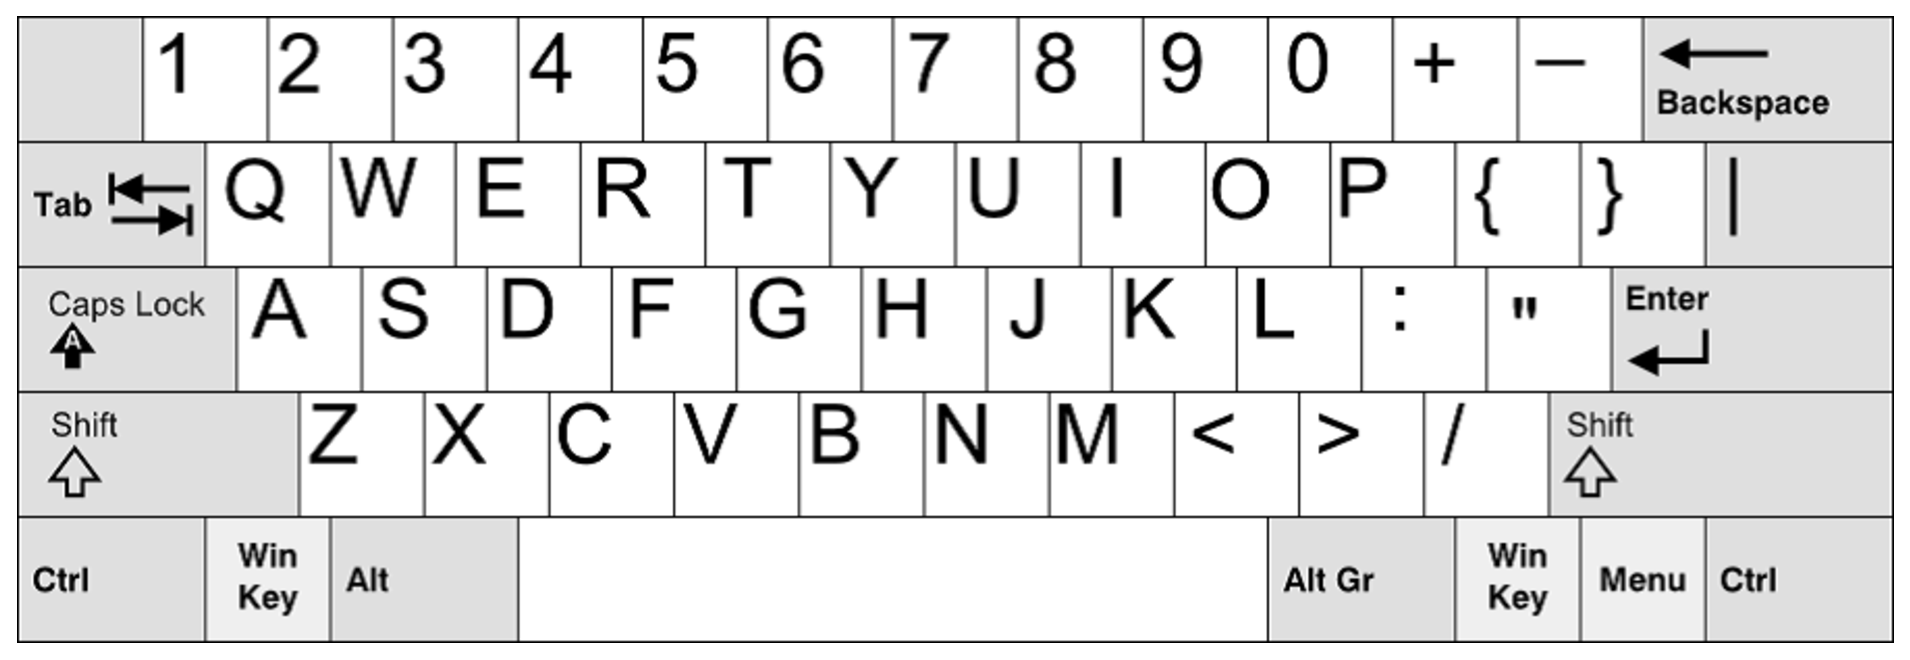
\includegraphics[width=14cm,clip]{res_tomoemon/qwerty.eps}
 \end{center}
 \caption{Qwerty�z��}
 \label{qwerty}
\end{figure*}

���̔z����g���ĉp�����̓��[�h��\key{Q}��������[q]�Ƃ����������R���s���[�^�ɓ��͂���܂��B�ǂ̃L�[���������Ƃ��ɉ��̕��������͂���邩�A�Ƃ����g�ݍ��킹���L�[�{�[�h�̘_���z��ƌ����A���̋L���Ŕz��ƌ������ꍇ�͂�����w���܂��B����A�����I�ȃL�[�̌`���ʒu���L�[�{�[�h�̕����z��ƌ����܂��B���݂̃L�[�{�[�h�̑����͊e�i�̃L�[�̈ʒu���������‰��ɂ���Ă��܂����A���ꂢ�Ȋi�q��ɂȂ��Ă��镨���z��̃L�[�{�[�h�����݂��܂��B

�����z��Ƙ_���z��̃C���[�W���킫�ɂ������͖����󃂃f���L�[�{�[�h\footnote{\url{http://www.pfu.fujitsu.com/hhkeyboard/hhkbpro2/nokeytop.html}}���C���[�W����Ɨǂ��ł��傤�B

\begin{figure*}
 \begin{center}
   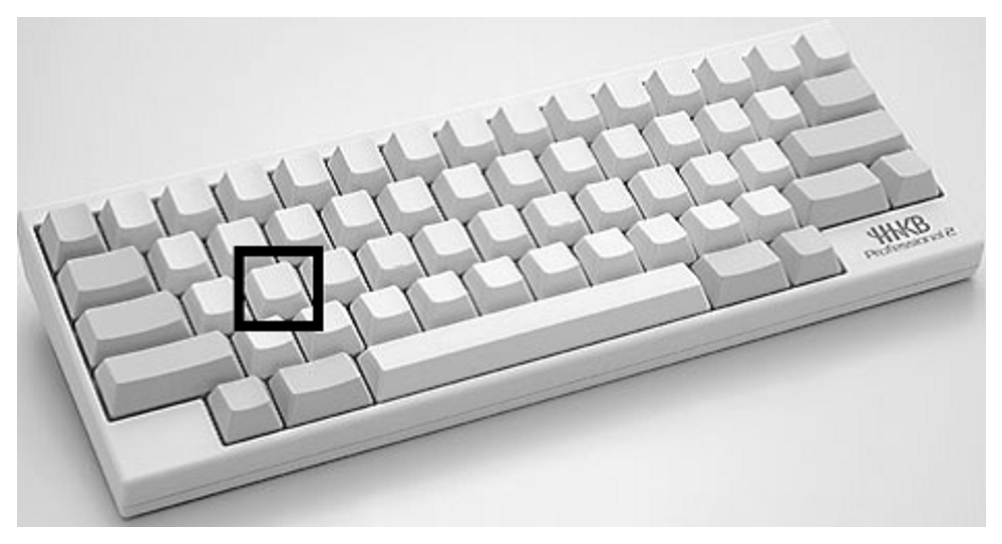
\includegraphics[width=14cm,clip]{res_tomoemon/nokeytop.eps}
 \end{center}
 \caption{Happy Hacking Keyboard Professional2 ���^������}
 \label{nokeytop}
\end{figure*}


�}\ref{nokeytop}�Ŏl�p���g�ň͂񂾈ʒu�̃L�[���������Ƃ��ɉ��̕������o�邩�͘_���z��ɂ���Č��܂�܂��BQwerty�z����g���Ă����[s]���o�܂����A�}\ref{dvorak}��Dvorak�z��ł�[o]�̕������o�܂��B

\begin{figure*}
 \begin{center}
   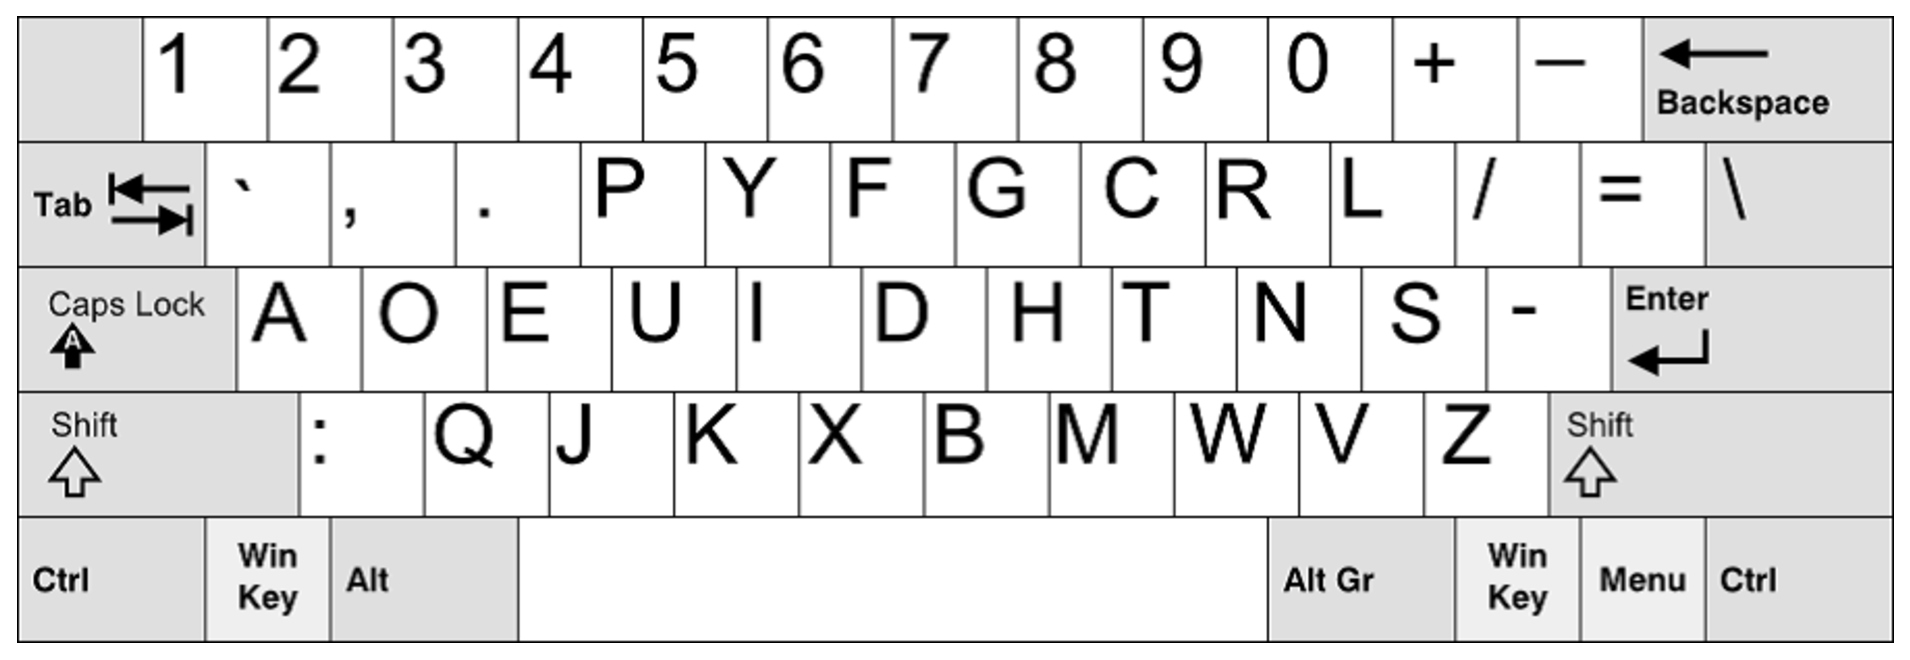
\includegraphics[width=14cm,clip]{res_tomoemon/dvorak.eps}
 \end{center}
 \caption{Dvorak�z��}
 \label{dvorak}
\end{figure*}

�����z��̏�ɂ͂����‚��_���z����d�˂邱�Ƃ��ł��A�Ⴆ�Ε����I�ȃL�[�{�[�h1���ŁAQwerty�̉p�����́A���ȓ��́A���[�}�����͂Ƃ����������̔z���؂�ւ��A�܂��͑g�ݍ��킹�Ď������邱�Ƃ��ł��܂��B�}\ref{arrangement}�͕����z��Ƙ_���z��̊֌W��\�������̂ł��B

\begin{figure*}
 \begin{center}
   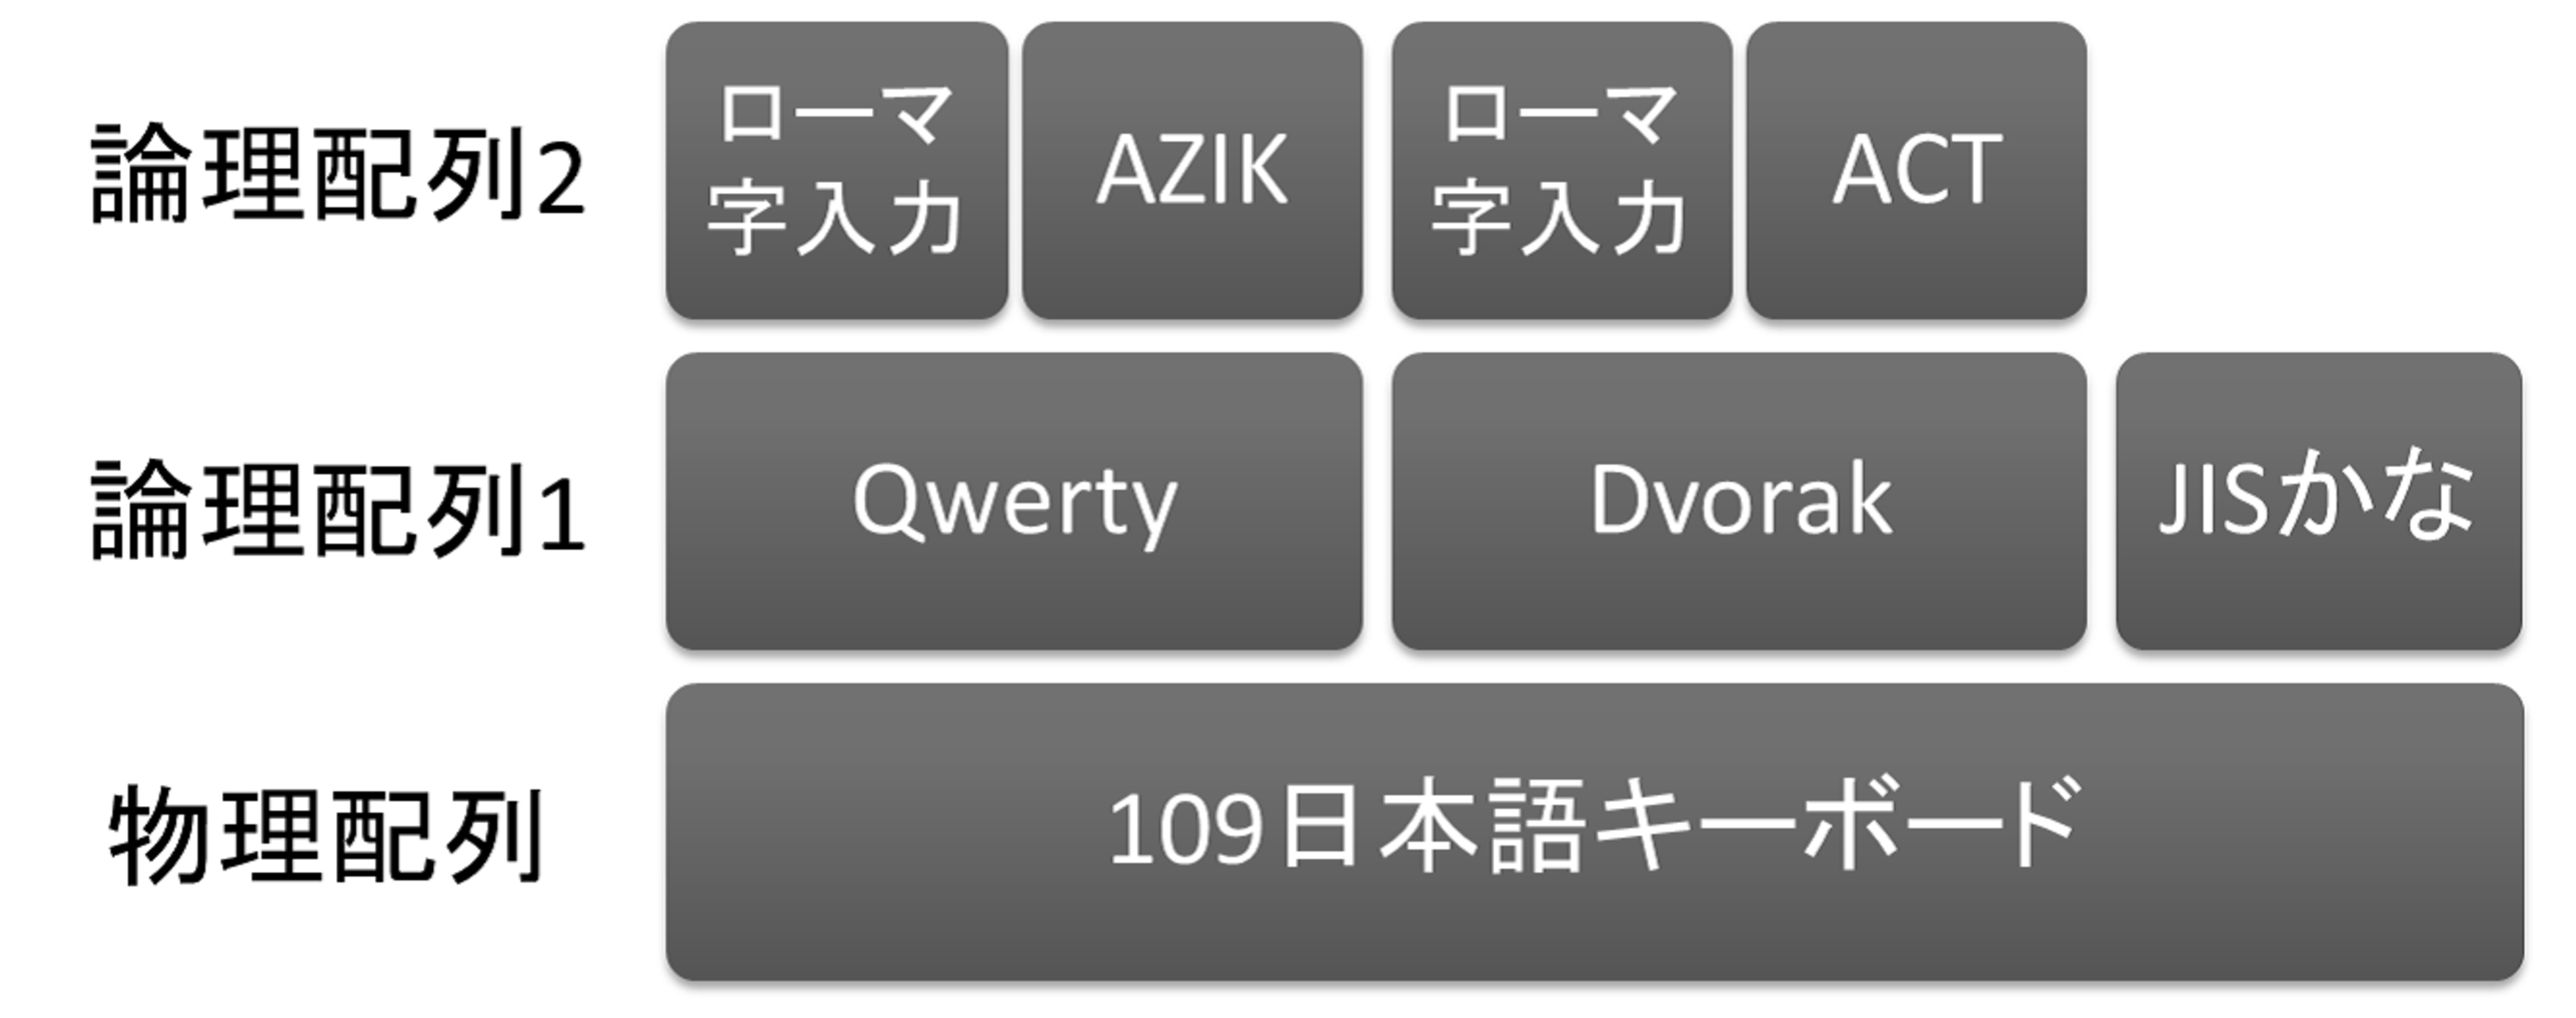
\includegraphics[width=14cm,clip]{res_tomoemon/arrangement.eps}
 \end{center}
 \caption{�����z��Ƙ_���z��̊K�w}
 \label{arrangement}
\end{figure*}

�_���z�����������ƕ�����ƁA�p������͂���z��Ƃ��Ȃ���͂���z��̓��ނɕ����邱�Ƃ��ł��܂�\footnote{�����𒼐ڂł���z�������܂��������ł͊������܂��B}�B���[�}�����͂��ŏI�I�ɂ͂��Ȃ���͂���z��Ȃ̂ŁA�����ł͂��ȓ��͂̈�‚Ƃ��܂��B�������A���[�}�����͉͂p���̑g�ݍ��킹�œ��͂��邽�߁A�}\ref{arrangement}�̂悤�ɉp�����͂̔z��Ɉˑ����Ă��܂��B

\subsection{���͑��x�ƑŌ����x}

����͓��ɓ�����Ƃ͂Ȃ��̂ł����A�u���͑��x�v�u�����v�u�x���v�Ƃ������t���悭�g���̂ŁA���ꂼ��̈Ӗ����m�F���Ă����܂��B�܂��A���͑��x���A[�ۑ�̕�����]��[���͂ɗv��������]�ƒ�`���܂��B���Z�^�C�s���O�ɂ����āA���͂��ׂ������͂��ׂė^�����Ă���̂ŁA������ۑ�̕�����ƌĂсA���̕��������u�ۑ�̕������v�Ƃ��܂��B�����ł͉p���A���ȁA���Ȋ���������Ȃǂ͋C�ɂ��܂���B�܂��A���͉”\�ȏ�ԂɂȂ��Ă�����͂���������܂ł̎��Ԃ��u���͂ɗv�������ԁv�Ƃ��܂��B��̗�Ő�������Ɓu����ɂ��́v��4�b�őł��؂����ꍇ�̓��͑��x��1.25����/�b�ł��B���͑��x���u�����v�Ƃ͂��̓��͑��x�̒l���傫�����ƁA�u�x���v�͂��̋t��\���܂��B
����Ƃ͕ʂɁu�Ō����x�v�Ƃ���������������ꍇ������܂��B����͒P���ŁA�P�ʎ��Ԃ�����ɃL�[�{�[�h�̃L�[������Ō��ł��邩��\�����̂ł��B��ʓI�ɍ����ɑŌ��ł�����������ȓ��͂ɂȂ�܂����A�ϊ�����̓��{����͑��x�������ꍇ�͕ϊ��ɑ�z�����l���Ō����x�ŗ���Ă��Ă����͑��x�ŏ���ꍇ���\���ɂ��肦�܂��B

\section{�Ȃ��z���ς���̂�}

���āA�悤�₭�{��ł����A���������Ȃ��z���ς��Ȃ���΂����Ȃ��̂ł��傤���B�}�C�i�[�z����D��Ŏg�����Ƃ���^�C�p�[������̂͂Ȃ��ł��傤���B��q����ʂ�z���ς���Ƃ����̂͑傫�ȘJ�͂�K�v�Ƃ��܂����A��J���Ĕz���ς��邩��ɂ͂���Ȃ�̃����b�g�����݂���̂ł��B

\begin{itemize}
 \item �w�̓����ɖ������Ȃ��Ȃ�
 \item ���w�Ō�������
 \item �����A�ł�����
 \item �w�̈ړ�����������
 \item �w�̈ړ��͈͂������Ȃ�
 \item �Ō��̉񐔂�����
 \item �������₷���w���d�_�I�Ɏg��
\end{itemize}
�����͂ǂ�������Ō��ɂƂ��ďd�v�ƍl������v�f�ŁA���������݂ɃR���g���[���ł���悤�ɂȂ�̂��u�z���ς���v�Ƃ�����@�ł��B�������z���ς��铮�@�̊̂Ȃ̂ŁA���[�}�����͂��ɏ������������Ă����܂��B

\subsubsection*{�w�̓����ɖ������Ȃ��Ȃ�}
�u�킴�킴�v��łꍇ�A�W���^�w�ł͖�w�Ə��w��\finger{21112111}�ƂȂ�܂����A����͔��ɑł��ɂ����p�^�[���ɂȂ�܂��B�z���ς��邱�Ƃł����������p�^�[�������炵�A�ł��₷���p�^�[���ɕς��邱�Ƃ��ł��܂��B
\subsubsection*{���w�Ō�������}
�u�ʂ��ʂ��v�Ƒłꍇ��\finger{77877787}�ƂȂ��āu�ʁv��ł‚��߂ɐl�����w��2�i�������܂����A���̂悤�Ȏw�̈ړ��͍�������������߁A�ł��邾�����Ȃ��ق����D�܂����ł��B
\subsubsection*{�����A�ł�����}
�u�Ȃ�́v�Ƒłꍇ�unannno�v�ƂȂ�A\key{N}��3��A���őł•K�v������܂����A�����L�[��A���őł‚̂��x���Ȃ�v���ɂȂ�܂��B���̏ꍇ�́unaxnno�v�Ƒł���1�񕪌��炷���Ƃ��ł��܂����A�������u�v������ꍇ�͔����邱�Ƃ��ł��܂���B
\subsubsection*{�w�̈ړ�����������}
�w���ړ����Ȃ��őł‚��Ƃ��ł���Γ��R�����Ȃ�܂�\footnote{�����w�œ����L�[��A�ł���ꍇ�͗�O�I�ɒx���Ȃ邱�Ƃ�����܂��B}�B�z��ɂ���Ă̓z�[���|�W�V��������قƂ�ǎw�𓮂������ɑłĂ邱�Ƃ������b�g�Ƃ��Ă����Ă�����̂�����܂��B
\subsubsection*{�w�̈ړ��͈͂������Ȃ�}
��L�ɋ߂��v�f�ŁA���ȓ��͂̏ꍇ��4�i�g���̂ɑ΂��A���[�}�����͂ł�3�i�����g��Ȃ��Ƃ������z�񂲂Ƃ̈Ⴂ������܂��B�L���͈͂��g������1�Ō��œ��͂ł��镶���̎�ނ������č������ł������A�w�̈ړ��͈͂��L���Ȃ邱�ƂŃ~�X�̏��Ȃ����肵�����͂�����Ȃ�Ƃ����꒷��Z������܂��B
\subsubsection*{�Ō��̉񐔂�����}
��菭�Ȃ��Ō��񐔂œ����������łĂ�悤�ɂ��邱�Ƃ��ł��܂��B���[�}�����͂́u����ɂ��́v��10�Ō��ł����A���ȓ��͂ł�5�Ō��ɂȂ�܂��B
\subsubsection*{�������₷���w���d�_�I�Ɏg��}
�E�����̐l�͓��R�E��̕����������₷���A�܂�������Ɋւ�炸�l�����w�⒆�w���������₷�����ƂƎv���܂��B�z��Ɠ��͂��镶�͂̑g�ݍ��킹�ɂ���Ă͂���ȊO�̎w�𑽂��g���Ƃ��������Ƃ��N���肦�܂��B���̏ꍇ�A���Ȏw����K�ɂ���Ēb����̂�����ł����A�������₷���w���d�_�I�Ɏg���z����g�����ƂŁA�S�̂��猩�Ă�荂���ɑłĂ�悤�ɂȂ�܂��B

�����̓����𓥂܂��A�e�l�ɂƂ��ēK�؂Ȕz��ɐ؂�ւ��邱�ƂŁu���͑��x�������v�Ȃ�܂��B�������A��̒��ł��������Ă���ʂ�A�����͕K�������z���ύX���邱�Ƃł��������Ȃ������b�g�ł͂Ȃ��A�䗬�^�w��������铙�́u�œK���v�e�N�j�b�N�ɂ���ăJ�o�[�ł���͈͂����X����܂��B�������A�Ⴆ�΍œK���ł͑Ō��񐔂����炷���Ƃ͂ł��܂���B�œK�������_��ɁA���Ž��R�ɏ�L�v�f�����P�ł���̂��z���ς���Ƃ�����@�ɂȂ�܂��B�z�񂲂Ƃɓ��ɂǂ̗v�f���d�����Ă��邩�قȂ邽�߁A�z���I������ۂ͎������d���������v�f�Ƃ̃}�b�`���O���d�v�ɂȂ�܂��B

���̏ꍇ��AZIK�Ƃ����z����x�[�X�ɂ������̂��g���Ă��܂��B���̔z��ł̓��[�}�����͂Ŋ��蓖�Ă��Ă��Ȃ��p���̑g�ݍ��킹�ɕʂ̂��Ȃ����蓖�ĂāA���̃��[�}�����͂͂قڈێ����‚A��菭�Ȃ��Ō��̑ł��₷���p�^�[���𑝂₵�Ă��܂��B�Ⴆ�Ε\\ref{tomoemon:compare_roman_azik}�̂悤�ȑł������ł��܂��B

\begin{table}
\begin{center}
\caption{���[�}�����͂�AZIK�̔�r}
\label{tomoemon:compare_roman_azik}
\begin{tabular}{ccc}
\hline
���� & ���[�}������ & AZIK \\
\hline
���� ���� ���� & kan kin kon & kn kk kl \\
���� ���� ���� & sha shu sho & xa xu xo \\
�ɂ� �ɂ� �ɂ� & nya nyu nyo & nga ngu ngo \\
�������� & gakkou & ga;kp \\
\hline
\end{tabular}
\end{center}
\end{table}

���̃��[�}�����͂̑啔�������̂܂܎g����Ƃ�����������A�ʏ�̃��[�}�����͂��g���‚��X�Ɍ����I�ȑł��������Ă������Ƃ��ł���Ƃ��������b�g�������܂����A����䂦�Ɍ��I�ȕω��͖]�߂Ȃ��Ƃ������ƂɂȂ�܂��B���������b�g�Ɗ��������f�����b�g�Ɗ����邩�́A�l���ꂼ��Ȃ̂ŁA�����̖ڎw�����̂Ɣz�񂲂Ƃ̓������悭�m�邱�Ƃ��d�v�ł��B

\section{�z���ύX���ׂ��łȂ�5�‚̗��R}

�����b�g�����������Ă��Ƃ͎��ȐӔC�łƂ����̂��s�e�؂Ȃ̂ŁA�z��ύX���ׂ��łȂ����R�����킹�Đ������Ă����܂��B���ۂ̂Ƃ��냁���b�g�ɂ‚��Ă͂��낢��ȂƂ���ŏЉ��Ă���̂ŁA�d�v�ɂȂ�̂̓f�����b�g�̕��������肵�܂��B�����Ȕz��Ƀ`�������W���ė~��������Ƃ��Ă͌g�ѓd�b�̗����v�����̂��Ƃ�菑���̂悤�ɋɏ��t�H���g�ŏ��������Ƃ���ł����A�f�����b�g������������ł̃`�������W�������߂��܂��B���āA��q�̂悤�ȃ����b�g�����󂷂邽�߂Ɏx�����R�X�g�ƃ��X�N�͏���������܂���B�قȂ�z����K�����邽�߂ɂ��Ȃ��͏��Ȃ��Ƃ����̓�‚��o�傷��K�v������܂��B
\begin{itemize}
 \item ���Ƃ��Ǝg���Ă����z��ɂ�������K���Ԃ̌���
 \item ���Ƃ��Ǝg���Ă����z��Ƃ̍����̉”\��
\end{itemize}
�܂��A�قȂ�z��K���Ɏ��g�ޏ�Ŏ��̂悤�ȍ���ɑ�������”\��������܂��B
\begin{itemize}
 \item ���K���@���m�����Ă��Ȃ�
 \item �����L���O�ւ̎Q��Ȃǂ��F�߂��Ȃ�
 \item ��p�̃\�t�g�𓱓����Ȃ���΂Ȃ�Ȃ�(Linux���Ŏg���Ȃ��”\��)
\end{itemize}
�܂��A���Ƃ̔z��ւ̉e���ł����A����܂Ń��[�}�����͂ŗ��K���Ă����l���u���ꂩ��͂��ȓ��͈�r�ł���Ă������v�ƌ��f�����Ƃ���ƁA���̏u�Ԃ����Ƀ��[�}�����͂̓��͑��x�͐����Ă����΂���ł��B�������A�����ɑłĂȂ��Ȃ邱�Ƃ͂���܂��񂵁A�����̓��͑��x���ێ��ł���ꍇ������܂��B�������A�z���؂�ւ������ƂŌ��̔z��̓��͑��x�����シ�邱�Ƃ͊�{�I�ɂ���܂���B��{�I�ɂƌ������̂́A���Ƃ��ƃ^�C�s���O���S�҂������ꍇ�Ȃǂ́A�ʂ̔z��ɐ؂�ւ��Ă�����K���d�ˁA������̔F�����x��w�̉^���\�͂����コ���邱�ƂŁA���̔z��ɖ߂����^�C�~���O�ňȑO��葬���łĂ�悤�ɂȂ��Ă��邱�Ƃ͏\�����肦�܂��B�������A���łɌ��E�Ɗ����鑬�x�܂ŗ��K���Ă���z���ύX�����ꍇ�ɁA�z���߂��đ����Ȃ邱�Ƃ͂܂�����܂���B

�͂��߂ɂ������܂������A�z���؂�ւ��邱�Ƃ͌��̔z��ɂ����鐬���̉”\�����̂ċ��邱�ƂƓ��`�ł��B���Ȃ������K�ɔ�₹�鎞�Ԃ�100�Ƃ��āA100�̎��Ԃ��ׂĂ����[�}�����͂Ɏg���Ă���Γ��B�ł�����������Ȃ��������̂ĂāA�ʂ̔z��ɓq����̂ł��B����́A�V�����z��̗��K���Ԃ�50�����Ƃ��āA�c��50�̓��[�}�����͂ɔ�₷�悤�ȏꍇ�����l�ł��B���[�}�����̗͂��K���Ԃ������ɂȂ邱�ƂŊm���Ƀ��[�}�����͂̐����͒x���Ȃ�܂��B

����ɉ����āA���Ƃ��Ƃ���Ă����z�񂪂���ɒx���Ȃ�v���Ƃ��ĐV�����z��Ƃ̍������������܂��B�����Ɋւ���m���͂��܂��ɏ\���W�܂��Ă���Ƃ͌����������󋵂ł����A�p���z�񓯎m(Qwerty��Dvorak��)�₩�Ȕz�񓯎m(JIS���Ȃƌ��z��)�A���[�}�����͌n���m(Qwerty��AZIK��)�ł͍�������������”\���������ł��B��������������ƗႦ�΁u����ɂ��́v��Qwerty���[�}�����͂őł��Ȃ��Ƃ����Ȃ���ʂŁAAZIK���Ɂuklnitiha�v�Ƒł��Ă��܂����Ƃ�����܂��B�ȑO��������Ƃ̂���z��Ɠ��n���̔z���V���ɏK�����悤�Ƃ���ꍇ�́A�ȑO�̔z�񂪎g���Ȃ��Ȃ邱�Ƃ��o�債�Ă����������ǂ��ł��傤�B

���ꂾ���ŏ\���n�[�h���������̂ł����A����ɗ���������Ȃ���΂Ȃ�Ȃ���������܂��B
���K���@���m�����Ă��Ȃ��z��̗��K������ۂ͎����Ō����I�ȗ��K���@���l����K�v������܂��B�Ⴆ�Ύ��̏ꍇ�AAZIK����K����ۂ́A�V���Ɋ��蓖�Ă�ꂽ���[�}���̑g�ݍ��킹�������Ȃ肷�ׂē������ė��K����͓̂�����߁A��‚����ԂɎ����ꂽ�P�����K���Ă����悤�ɂ܂����B�܂��A�򒹔z��ł̓V�t�g�L�[���g���ꍇ�Ƃ����łȂ��ꍇ�𕪂��ė��K���s���܂����B����܂łɎ��g�񂾔z��Ɨ��K���@�ɂ‚��Ă͌�q���܂��B

����ɁA���Ȃ����I�񂾔z��̓^�C�s���O�\�t�g�̃����L���O����ւ̎Q�킪�F�߂��Ȃ��”\��������܂��B�Ⴆ�΁A�^�C�v�E�F���ɂ�����AZIK�͎Q�l�L�^�����ƂȂ��āA�ʏ�̃����L���O�Ɠ��������ɂ͂Ȃ�Ȃ����Ƃ���������Ă��܂��B�܂��A�����p�\�R�����̓R���N�[���̏ꍇ�́A�e�Q���҂̎���ő�����s���\�I�ł͊e��z�񂪑I���”\�ł����A������ł͊�{�I�ɂ̓��[�}�����͂����ȓ��͂����I���ł��܂���B���p�\�̂悤�Ȍ��I�ȑ��ɂ����Č���F�߂��Ă��Ȃ��z��ł̎Q����F�߂����邱�Ƃ͑傫�ȍ���𔺂��ł��傤�B

���p�\�̂悤�ȑ��œ���z�񂪎g���Ȃ������̈�‚ɂ��Ȃ��Ă���̂��A�z��ɂ���Ă͐�p�̃\�t�g�E�F�A�𓱓����Ȃ���Ύg�����Ƃ��ł��Ȃ��Ƃ����_�ł��B��p�̃\�t�g�Ƃ����Ă���{�I�Ƀt���[�\�t�g�œ����������܂œ���Ȃ����߁A�����������Ă��܂��Ί�{�I�ɖ��͂Ȃ��̂ł����A��p�\�t�g���K�v�ɂȂ邱�ƂŎ��̂悤�Ȗ�肪�N���肦�܂��B
\begin{itemize}
 \item OS�̃o�[�W�����A�b�v�ɂ�肱��܂Ŏg���Ă����\�t�g���g���Ȃ��Ȃ���
 \item �قȂ�OS�������Ă���PC�Ŏg���Ȃ�����
 \item ��Ђ�PC�ȂǑ��̊‹��œ����z����g���������\�t�g�𓱓��ł��Ȃ�
\end{itemize}
�ň��̏ꍇ�A�u����ł͐e�w�V�t�g���g���Ă��邯�lj�Ђł̓��[�}�����͂��g��Ȃ��Ă͂Ȃ�Ȃ��v�Ƃ������ꍇ�͏\���ɂ��肦�܂��B���������Ӗ��ł��z�񓯎m�̍����̉”\���ɂ͏\�����ӂ���K�v������A�܂��A�������g���”\���̂���PC�ɐ�p�\�t�g�������邩�͎��O�Ɍ������Ă����ׂ��ł��B


\section*{�z��ύX�̋�̗�}

���̏͂���͎����g�̔z��ύX�̌o���ɂ‚��ďЉ���Ă��������܂��B�����܂łł��łɏ����Ă��镔��������܂����A�z���ύX����ɂ������Č����������ƁA���ۂɕς��Ă݂Ċ��������ƁA���������邽�߂ɍH�v�������ƂȂǂ�U��Ԃ�A�݂Ȃ���̔z��ύX�̎Q�l�ɂ��Ă���������΂Ǝv���܂��B

�\\ref{tomoemon:history}�͎�������܂łɌo�������z��N�\�ɂȂ�܂��B���B���x�̓^�C�v�E�F������R�A����K�ɂ������{��p�ꃂ�[�h�̃����N�ŕ\���Ă��܂��B
\begin{table}
\begin{center}
\caption{�M�҂�����܂łɌo�������z��}
\label{tomoemon:history}
\begin{tabular}{ccc}
\hline
�z�� & ���K���� & ���B���x \\
\hline
Qwerty���[�}�� & 1997�`2009 & ZI \\
JIS���� & 2001�`2003 & XA \\
Dvorak���[�}�� & 2004 & D \\
�Ў�`���C����(�E��) & 2005 & SF \\
�򒹔z��290 & 2005�`2008 & XS \\
AZIK & 2008-2009 & XX \\
tomoemon-AZIK\footnotemark & 2009�` & ZH \\
\hline
\end{tabular}
\end{center}
\end{table}
\footnotetext{�M�҂ɂ��AZIK�̓Ǝ�����}
���̒��œ��ɐe�w�V�t�g�n�ł���򒹔z��ƃ��[�}�����͌n�ł���AZIK�̌o���ɂ‚��ďЉ���Ă��������܂��B

\section{�z��ύX�̗�1 - �򒹔z��}

\subsection{����}

�e�w�V�t�g�n�̔z��ł��B�}\ref{asuka}\footnote{�}�� \url{http://ameblo.jp/asuka-layout/entry-10334710008.html} ���}�̂悤��1�‚̃L�[�ɕ����̂��Ȃ����蓖�Ă��Ă��āA����L�[�������ۂɐe�w�V�t�g�𓯎��ɉ����������Ȃ����œ��͂��邩�Ȃ�؂�ւ��܂��B�u�e�w�V�t�g�Ȃ��ʼn����v�A�u���e�w�V�t�g�������Ȃ��牟���v�A�u�E�e�w�V�t�g�������Ȃ��牟���v���Ƃ�1�‚̃L�[��3��ނ̂��Ȃ���͂��邱�Ƃ��ł��܂��B�e�w�V�t�g�̑�\�i�ł���NICOLA�Ƃ̑傫�ȈႢ�͐e�w�V�t�g�̃��[���I�[�o�[�ł��B�򒹔z��ł́A�e�w�V�t�g�L�[���������ςȂ��ŃL�[�𕡐������Ă����ƁA���ׂẴL�[�Őe�w�V�t�g���K�p���ꂽ���Ȃ��o�͂���܂��BNICOLA�ł͂��Ƃ������e�w�V�t�g�L�[���g��2��������͂���ꍇ�ł��A1�����ڂʼn������e�w�V�t�g���������񗣂��Ă��������x�����K�v������܂��B


\begin{figure*}
 \begin{center}
   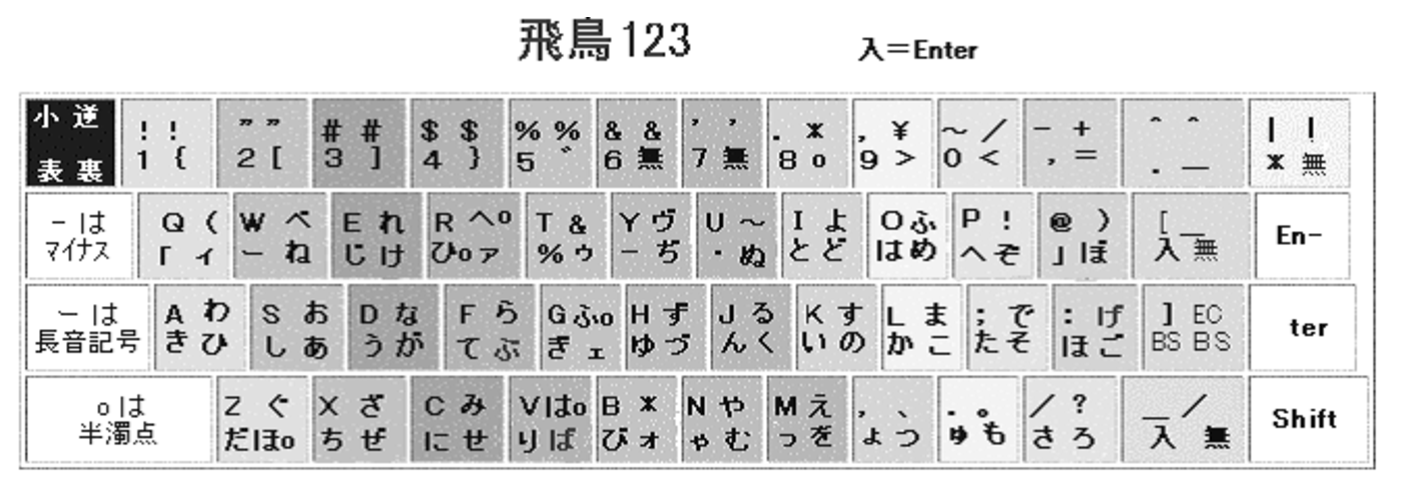
\includegraphics[width=14cm,clip]{res_tomoemon/asuka.eps}
 \end{center}
 \caption{�򒹔z��123-383��}
 \label{asuka}
\end{figure*}

\subsection{���@}

���̎����ɔ򒹔z����n�߂����R���ӏ������ɂ���ƈȉ��̂悤�ȓ��e�ɂȂ�܂��B
\begin{itemize}
 \item Qwerty���[�}�����͂̐����Ɍ��E�������Ă���
 \item ���{����͂ɂ����Ă̓��[�}�����͂ɔ�ׂĂ��ȓ��͂̕��������͖̂��炩
 \item JIS���Ȃ͉ߋ��Ɏ��g�񂾌���4�i�g�������������ɍ���Ȃ�
 \item ���܂��ܔ򒹔z����Љ�Ă������
\end{itemize}
1�–ڂ͂ǂ��炩�Ƃ����Ə��ɓI�ȗ��R�ŁA�܂��ɖ{�L���́u�͂��߂Ɂv�ŏq�ׂ��󋵂ɂ����āA���ɂ�������悤�ȋC�����ő��̔z�������Ă݂悤�Ǝv���܂����B���U��Ԃ��Ă��AQwerty���[�}���ł����Ɨ��K����΃^�C�v�E�F���ɂ�����ō������N�͂��������グ�邱�Ƃ͂ł���Ǝv���܂����A�����̎��_��Qwerty���[�}�����͂̑ł��ɂ����������ڂɂ‚��Ă������߁A�����ɂ��̗��K������C���N�����A�����ς�Ƃ�����̉”\���͐؂�̂Ă܂����B

2�–ڈȍ~�̗��R�ɂ‚��āA���ȓ��͂ƈꊇ��Ɍ����Ă�JIS���Ȃ�򒹔z��ȊO�ɂ������̔z�񂪑��݂��Ă���A�������򒹔z���m��O�Ɍ��z����Љ��Ă����̂ł����A���Ƃ��Ɛe�w�V�t�g�ɋ����������Ă������Ƃ���򒹔z��Ɍ��߂܂����B�̂̃��[�v�����̓R���e�X�g�ł͐e�w�V�t�g���̗͂��p�҂����𑍂Ȃ߂ɂ��Ă����A�Ƃ����悤�Șb���悭�����Ă������Ƃ���A���R�Ɛe�w�V�t�g�͂������Ƃ�����ۂ�����܂����B����ŁA�e�w�V�t�g�ɂ‚��Ē��ׂĂ݂�ƁA�V�t�g���s�������Ō������珜���Ă����������ɏ��Ȃ��Ō����ŏЉ��悤�ȗႪ���X����A�኱�����񂭂����ȂƂ�����ۂ������Ă��܂����B
��X�ɂȂ��Ē��ׂĂ݂��Ƃ���ł́A�O�҂ɂ‚��Ă͕p�o�P��������o�^�̂悤�Ȍ`�œo�^���Ă��������̂悤�ł���A���ǃ^�C�p�[�����߂�悤�ȓ��͑��x��e�ՂɎ����ł�����̂ł͂Ȃ����Ƃ��킩���Ă��܂��B

���̂悤�ɁA�e�w�V�t�g���g�����Ƃň��|�I�ȑ��x��������킯�ł͂Ȃ��Ƃ����F�������߂��炠�����̂ł����A�����̒m�����^�C�p�[���e�w�V�t�g�Ō��E�t�߂܂ŗ��K������𕷂������Ƃ��Ȃ������̂ŁA�`�������W���[�Ƃ��Ă���Ă݂����Ƃ����C�����������ɂ������z��I���������Ǝv���܂��B

\subsection{���K���@}

�ߋ��̔z��K�����̗��K�͂��ׂāu�����Ȃ�^�C�v�E�F�����N�����đł��n�߂�v�Ƃ����ɂ߂ĒP���ȗ��K���@�������̂ł����A�򒹔z��ł�1�‚̃L�[��3�‚̂��Ȃ����蓖�Ă��Ă���A���̗��K���@�ł͂Ȃ��Ȃ��L�[�̈ʒu���o�����Ȃ��Ǝv���A�ꕔ�̃L�[��e�w�V�t�g�������g�����P������Ԃɗ��K���Ă����Ƃ������@�����܂����B

���̍ہA�u�򒹂̂��߂Ɂv�Ƃ����P��W�������Ă��������A�ȉ��̂悤�ȃp�^�[���ŗ��K���s���܂����B����5,6,7�Ɛi�ނɂ‚�ĕp�x�̒Ⴂ�������܂񂾒P��ɂȂ��Ă����܂��B
\begin{itemize}
 \item ����1: �V�t�g�����z�[���|�W�V����
 \item ����2: �u�ł��v�u�܂��v�u����v���̕����ƘA���V�t�g�̌�
 \item ����3: �V�t�g����z�[���|�W�V����
 \item ����4: �E��̏㉺�i�i�����Ƒ�����\ruby{�X��}{�悤����}���܂ށj���K������
 \item ����5-7: 1�`4�ȊO�̂���
 \item ����8: 1���[�h���ɃV�t�g�̐؂�ւ����������
\end{itemize}
���̗��K���@�͏��߂��炷�ׂĂ̂��Ȃ���������ɍ������P��̗��K������������Ȃ�������ǂ��A���̌��AZIK�̗��K�̍ۂɂ�������Ă��܂��B
�Ƃ����̂��A���߂ė��K����z��ł�1�������͂��邽�тɖ��񂩂Ȃ�z��}�̒�����T�����ƂɂȂ�܂��B�T���Ă͑ł��A�T���Ă͑ł������x���J��Ԃ��ď������“��Ƒ̂Ɋo�����܂��Ă����̂ł����A���ׂĂ̂��Ȃ��܂񂾒P�����K���Ă���Ɣz��}�̒����炩�Ȃ̈ʒu��T�����Ԃ����ɒ����Ȃ�܂��B�A���t�@�x�b�g�ł����26�‚���T���΂悢�����ł����A�򒹔z��̏ꍇ��70�ȏ�̂��Ȃ���T���Ȃ���΂Ȃ�܂���B
�v���O���~���O�̐��E�ł����������Ƃ����ĕ��G�Ȗ��𕪉����Ă����āA�ł��邾���P���ȕ��@�ʼn������‚���Ƃ����l����������܂����A�z����K������ۂ��ł��邾�����K�Ώۂ̔z��𕪊����ĒP���ŊȒP�ȗ��K�ɂȂ邱�Ƃ�S������̂��ǂ��ł��傤�B


\subsection{���K����}

�ŏI�I��2008�N�̒i�K�Ń^�C�v�E�F������K�Ŋ�{��p��XS�A����XA�ɓ��B���܂����B�ŏI�I�ɂƏ������̂͑��x�ʂł͂��ꂪ�قڌ��E�ŁA����ȏ�̑��x�����肵�ďo�����Ƃ͓���Ɣ��f��������ł��B2011�N���݂Ń^�C�v�E�F������K�̊�{��p��1�ʂ̃����N��ZD�ł��邱�Ƃ��l����ƁA�����ɂ��y�΂Ȃ������Ƃ����̂��q�ϓI�Ȏ����ł��B�X�l�̔\�͂̍������邽�߁A���ȊO�̃^�C�p�[�����g�߂΂����Ə�ɍs����”\���͂���܂����A��͂�e�w�V�t�g���g���Ƃ������������Ɗ����܂����B

JIS���ȓ��͂⃍�[�}�����͂Ƒ傫���Ⴄ�̂́A��͂�e�w���g���ăV�t�g�L�[�𑼂̂��ȃL�[�Ɠ����ɉ�������ł��B�z��ύX�\�t�g�̐ݒ�ɂ���ẮA�e�w�V�t�g�������Ă��炩�Ȃ������ꍇ�����ł͂Ȃ��A�t�ɂ��Ȃ������Ă���e�w�V�t�g���������ƂŃV�t�g���K�v�ȕ�������͂ł��܂��B����̓V�t�g�������^�C�~���O�ɋ��e�ł���덷���܂߂Ă����Ƃ������ƂȂ̂ł����A���̌o���ł͍����ɑłĂ�悤�ɂȂ��Ă���Ƃ��̋��e�덷�ɂ��~�X�������������߁A�u�e�w�V�t�g�������Ă��炩�Ȃ������ꍇ�ɂ̂݃V�t�g��L���ɂ���v�ݒ�ŗ��K���Ă��܂����B�������A����ł����͑��x�������Ȃ�΂Ȃ�قǐe�w�V�t�g�������^�C�~���O���V�r�A�ɂȂ��Ă��邽�߁A�V�t�g�̂���ɂ��~�X�̔����������ɂȂ�܂��B����͔򒹔z��Ɍ��炸�e�w�V�t�g�n�S�ʂɌ�����̂ł͂Ȃ����Ɗ����܂����B

��L�̒ʂ�A�򒹔z��̎��g�݂͑��x����Ƃ����ϓ_���猾���Ύ��s�ł��B
�������͂������̐e�w�V�t�g�̓����ɂ‚��Ă�����x�c���ł����A�z��K���̌����ǂ����K���@�ɂ‚��Ċw�Ԃ��Ƃ��ł����Ƃ��������b�g�͂���܂������A����ŗǂ������Ɣz��K�����J��Ԃ��Ă����͂����̔z��}�j�A�ɂȂ��Ă��܂��܂��B�{�C��(���Ȃ��Ƃ��Z���Ԃ�)�g�b�v�^�C�p�[��ڎw���l�ɂƂ��Ă͂��̂悤�Ȏ��g�݂͔����������ǂ��ƒf�����܂��B�����ɍł��K������‚̔z��ɂ��ׂĂ̗��K���Ԃ𒍂����ނ��Ƃ������A���͑��x��b�����Ԃ̕��@������ł��B


\section{�z��ύX�̗�2 - tomoemon-AZIK}

\subsection{����}

AZIK�͂��łɏЉ���Ƃ���AQwerty���[�}�����͂��x�[�X�ɂ��ďȑŌ����̓��[����lj������z��ł��Btomoemon-AZIK��AZIK�̃��[�����قڂ��̂܂܎g���‚A����ɓƎ��̏ȑŌ����[����lj������z��ɂȂ�܂��B���ɁA�\\ref{tomoemon:compare_roman_azik_tomoemon_azik}�̂悤�Ɂu���v�u�ށv�Ƃ��������Ȃ���͂���ۂɔ������铯�w�Ō����ł��邾��������p�^�[����lj����Ă���̂������ł��B
\begin{table*}
\begin{center}
\caption{���[�}�����́AAZIK��tomoemon-AZIK�̔�r}
\label{tomoemon:compare_roman_azik_tomoemon_azik}
\begin{tabular}{cccc}
\hline
���� & ���[�}������ & AZIK & tomoemon-AZIK \\
\hline
�ނ� �ނ� �ނ� & muta muti mutu & mfta mfti mftu & mta mti mtu \\
���� ���� ���� & kita kiti kitu & kfta kfti kftu & kta kti ktu \\
\hline
\end{tabular}
\end{center}
\end{table*}


\subsection{���@}

�򒹔z��̎��Ɏ��g�񂾔z��AZIK�ŁA�����I�ɂ͔򒹔z��ő���XA���o�������N��Ɏn�߂Ă��܂��B�ڂ������@�ɂ‚��Ă͎��̓����̓��L�����Ԃ��Ă������Ă��Ȃ��̂Ŋm���Ȃ��Ƃ͏����Ȃ��̂ł����A�����炭�򒹔z��̗��K�o�����琶�܂ꂽ���̓�_���傫�ȗ��R�������Ǝv���܂��B�򒹔z��̏K���܂łɎ��Ԃ����������̂ŁA�w�K�R�X�g���Ⴛ���Ȃ��̂ɐH�w���������̂���_�B������_�͔򒹔z��͐e�w�V�t�g�Ƃ����V���ȓ����ɂ���đ��x�̐������������Ă��܂������A�����̔z������P���č�����z��Ȃ�Ώ]�����������Ȃ�̂͂قڊm���ł��낤�Ƃ������ƁB
���̂悤�ɍl����ƁA���Ƃ���AZIK�Ɋ֐S�������Ă������Ƃ�����A�򒹔z��̂��Ƃ�AZIK��I�񂾂͕̂K�R�������̂�������܂���B

\subsection{���K���@}

\subsubsection*{�p�^�[���������K}
�򒹔z��̗��K���Ɠ��l�ɁAAZIK�ł��V���ɒlj����ꂽ�ȉ��̃p�^�[�������Ԃɗ��K���Ă������@�����܂����B

\begin{itemize}
 \item �w���x��p�L�[
 \item �w�V���x�w�`���x�s�L�[�A�����L�[
 \item �w����x\ruby{����}{�͂‚���}�g��
 \item �w�@���x�w�D���x�w�F���x�w�H���x
 \item �w�[�x�����݊��L�[
 \item �u�x�v�̑���́u�f�v
 \item �u�y�v�̑���́u�m�v
 \item �u�t�v�u�h�v���̑���́u�e�v
 \item �O����̓��́i�O������͊g���j
\end{itemize}

���ꂼ��ȉ��̂悤�ȒP�����K���Ă��܂��B
\subsubsection*{�p�^�[��1�F�w���x��p�L�[}
�u���v��\key{;}�̃L�[�P�Ƃœ��͂��邱�Ƃœ��w�Ō������炵�܂��B
\begin{itemize}
 \item �o�b�O [ba;gu]
 \item �J���b�g [kara;to]
\end{itemize}

\subsubsection*{�p�^�[��2�F�w�V���x�w�`���x�s�L�[�A�����L�[}
�u����v�s�́ux�v�A�u�`���v�s�́uc�v���q���Ƃ��Ďg���A�usha�v�ucha�v�ȂǂƔ�ׂĈ�Ō����炷���Ƃ��ł��܂��B
\begin{itemize}
 \item ���傤���� [xousei]
 \item �������� [ataxa]
\end{itemize}

\subsubsection*{�p�^�[��3�F�w����x�����g��}
���Ɂu��v�����������͖{���̕ꉹ�L�[��1�‰����g���܂��B�u����v�̏ꍇ��\key{O}��1�‰���\key{L}���g����\key{M}\key{L}�Ƒł‚��Ƃň�Ō����炷���Ƃ��ł��܂��B
\begin{itemize}
 \item ���񂾂� [mldai]
 \item �݂�� [mkna]
\end{itemize}

\subsubsection*{�p�^�[��4�F�w�@���x�w�D���x�w�F���x�w�H���x}
�����p�x�ŏo������ꉹ�̘A�����ЂƂ܂Ƃ߂ɂ����p�^�[���ł��B�u�q���{ai�v���u�q���{q�v�A�u�q���{uu�v���u�q���{h�v�A�u�q���{ou�v���u�q���{p�v�Ƃ��������[�}���Ɋ��蓖�Ă邱�Ƃ�1�Ō����炵�܂��B
\begin{itemize}
 \item �����Ƃ� [gptp]
 \item �悤���� [ypkq]
\end{itemize}

��L�̂悤�ȃ��[�}���̃p�^�[���ɑ΂��āA���ꂼ�ꃏ�[�h�𐔕S�‚��’��o����WeatherTyping�ŗ��K����Ƃ������@�����܂����B�e�p�^�[���ɂ‚��Ă̗��K�e�L�X�g���蓮�ō���Ă����̂��ʓ|�������̂ŁA�u�z��K����tomo�v�Ƃ����e�L�X�g���o�t�B���^�\�t�g���쐬�����̂ŁA�����̂�����̓O�O���Ă݂Ă��������B�\�t�g���̂Ŏ����t�@�C���������Ă��āA�w�肵���p�^�[���̃��[�h�������I�ɒ��o���邱�Ƃ��ł��܂��B

\subsubsection*{�p�^�[���œK�����K}
AZIK���K�œ���|�C���g�̈�‚��P���ɐV�����lj����ꂽ���[�����ق��ق��g���Ă���Ηǂ��킯�ł͂Ȃ��Ƃ����_�ł��B�ǂ��������Ƃ��Ƃ����ƁA�V�����lj����ꂽ���[�����g���ƁA�t�ɑł��Â炭�Ȃ��Ă��܂��ꍇ������Ƃ������Ƃł��B�Ⴆ�΁u�M�K�o�C�g�v�Ƃ����������ł‚Ƃ��͎��̂悤�ɂȂ�܂��B

\begin{itemize}
 \item AZIK: �M�K�o�C�g [gigabqto]
 \item Qwerty: �M�K�o�C�g [gigabaito]
\end{itemize}

�茳�ŏ��������Ă݂ė~�����̂ł����A\key{B}����\key{Q}�ɏ��w��L�΂��̂����‚��AQwerty���[�}�����͂̒ʂ�ɑł����ق����y�ɂȂ邱�Ƃ��킩��܂��B�������A�l�ɂ���Ă�AZIK�̃p�^�[���̕����ł��₷���Ƃ����������邩������܂��񂪁A����܂Ŏg��Ȃ��L�[�����[�}�����͂Ŏg�����Ƃɂ���āA�t�Ɏw�̓��������‚��Ȃ��Ă��܂��p�^�[���Ƃ����̂����݂��܂��B
�ǂ̃p�^�[�����ǂ̏ꍇ�Ɏg���āA�ǂ̏ꍇ�Ɏg��Ȃ��̂������ɂ߂�̂�AZIK�̗��K�ł͔��ɏd�v�ɂȂ�܂��B

���̏ꍇ�͊e��^�C�s���O�\�t�g�ŗ��K���Ă�������AZIK�̃p�^�[���ʂ�ɑł‚Ƒł��ɂ����Ȃ�p�^�[����\\ref{tomoemon:later_azik}�A�\\ref{tomoemon:non_azik}�̂悤�ɂ܂Ƃ߂Ă����܂����B����Ɋւ��Ă͐l�ɂ���đ傫�������o��̂ŁA�݂�Ȃ��݂�Ȃ��̂Ƃ���ɂȂ�킯�ł͂���܂���B���ہA�u���O�ɑł��ɂ����p�^�[������������u�����v�́uss�v�̕��������Ƃ����������܂����B�����AAZIK�̗��K������ۂ͂��̂悤�Ȏ��������ȃp�^�[���͋C�Â�����܂Ƃ߂Ă����A�ł��邾���g��Ȃ��悤�ɂ��邩�A���邢�͔O����ɗ��K���邱�Ƃ�S������̂��ǂ��ł��傤�B

\begin{table*}
\begin{center}
\label{tomoemon:later_azik}
\caption{AZIK�g�����g�����Ƃ�Qwerty�����x���Ȃ�p�^�[��}
\begin{tabular}{cccl}
\hline
���� & AZIK & ���[�}������ & �⑫ \\
\hline
���� & ss & sei & \\
�f�B�X�N & dcisuku & dhisuku & ��X [dyi] �Łu�ł��v��łĂ�悤�ɕύX \\
�e�B�[ & tgi- & thi- & ��X [tyi] �Łu�Ă��v��łĂ�悤�ɕύX \\
�X�|���W & suplji & suponji & �������K�������猋�\�ł��₷���Ȃ��� \\
�A���P�[�g & annke-to & anke-to & ��X�u@�v�ł��u��v����͂ł���悤�ɕύX \\
XaXai: �킩���� & wakq & wakai &  \\
�ۂ��� & po;to & potto & �E�菬�w����� \\
\hline
\end{tabular}
\end{center}
\end{table*}

\begin{table*}
\begin{center}
\label{tomoemon:non_azik}
\caption{���ɑI����������A��{�I�ɂǂ̏�ʂł��g��Ȃ���������AZIK�g��}
\begin{tabular}{ccl}
\hline
���� & AZIK & �⑫ \\
\hline
���� & ss & ���w�Ō��ɂȂ�̂�sei�̕����ǂ� \\
x��: ��� & wz & wn�̕����ł��₷�� \\
�΂� & bq & ���ʂ�bai�̕����y \\
\hline
\end{tabular}
\end{center}
\end{table*}

���̓_���番����ʂ�AAZIK�͈�‚̕�����̑ł‚ɂ��Ă�Qwerty���[�}�����͂ɔ�ׂđ����̑ł��������݂��܂��B���߂̂����͂ǂ̃p�^�[�����ǂ̏�ʂŎg�����𓪂ň�ˆ�Šm�F���ė��K����K�v������A�����ȃ^�C�s���O��ڎw���Ȃ�΂����̂Ɋo�����܂��Ȃ���΂Ȃ�܂���B

\subsection{���K����}

Qwerty���[�}�����͂����P�����z��Ȃ̂�����A�K�������Ȃ邾�낤�ƊÂ����ʂ��������̂ł����A���ۂɃ^�C�v�E�F���̋L�^�����S�ɓh��ւ���ꂽ�̂�1�N�ȏ�o�������Ƃł����B�Ƃ����Ă��A�����݂�����Ɨ��K���Ă����킯�ł͂Ȃ��^�C�v�E�F�����v���C���������ł����Ɩ�90���ɂȂ�܂��B

���Ԃ����������̂͂�͂���K���@�̍��ɏ������A�ǂ̃p�^�[�����ǂ��Ŏg������̂Ɋo�����܂���_�ł��B�܂��AAZIK����tomoemon-AZIK�ւ̑啝�ȃp�^�[���lj��̌����Ƃ������A�{���̔z����K���班�����ꂽ�ӏ��ł����Ԃ�v���܂����B�z��̉����́A��x�n�߂�Ǝ������[������`�ɂȂ�܂łɎ��Ԃ������邱�Ƃ������āA�K�����������^�C�s���O��ڎw���l�ɂ������߂���킯�ł͂���܂��񂪁A���̏ꍇ�͌��ʓI�ɔ��ɖ����̂����z��ɂł����Ǝv���Ă��܂��B
�����ł��������Ƃ͓��R���Ɂu��葬���ł‚��Ƃ��ł���v���Ƃł���A����Ɂu�ł��₷���Ȃ����v�Ƃ������Ƃł�����܂��B����܂łɏK�������z��͂��ׂă^�C�s���O�\�t�g�őł‚��߂̔z��ł����Ȃ������̂ł����Atomoemon-AZIK�����ɑł��₷�����Ƃ�����A���݂͎d����u���O�������Ƃ�����PC���g�����ׂĂ̏�ʂł��̔z����g�p���Ă��܂��B
���Z�^�C�s���O�ɂ����鍂������ڎw����ŕK���������p�ʂ̑ł��₷�����d������K�v�͂���܂���B�Ȃ��Ȃ�A���Z�^�C�s���O�͊�{�I�ɃR�s�[�Ō��ŁA���p�ʂł͊�{�I�ɑn��Ō��Ƃ����傫���قȂ�X�^�C��������ł��B�����g�����Ƃ��Ɠ���ɂ�����g�p�܂ōl���Ă����킯�ł͂Ȃ��̂ŁA���̌��ʂ͋��R�̎Y���ƌ����Ă����ł��傤�B�����AAZIK�𓱓�����̏�Ő�p�\�t�g���K�v�Ȃ��Ƃ����_���ePC�ɓ������₷���Ƃ��������b�g�𐶂�ł���̂͊m���ł��B


\section{�ǂ�����Ĕz���I�����ׂ���}

�����܂Ŕz��K���̎��s����ɂ‚��ďЉ�Ă��܂����B���ꂩ��V���ɔz����K�����悤�ƍl���Ă���l�́u�ߋ���A�z�������Ă����l�͔z��X�AB�z�������Ă����l�͔z��Y�v�̂悤�ȁu�z��I���t���[�`���[�g�v�����҂���Ă�����������܂���B�������ɂ����������̂�����Ε֗��ł����A����܂Ő������Ă����ʂ�ǂ̔z������ɕ��G�ȓ����������Ă��܂��B�V���ɏK������l�ɂ���Ă���ɐV�������������‚���”\��������܂��B����ɁA�K�����悤�Ƃ���l�̓��ӂȎw�̓����Ƃ������悤�ɐl���ꂼ��̓���������܂��B�����_�ł��̗��҂�g�ݍ��킹���t���[�`���[�g�����͓̂���̂ŁA�����̎��������ǂ�ł��邠�Ȃ��ɂ��C���������Ǝv���܂��B

�t���[�`���[�g�͒񋟂ł��܂��񂪁A����܂ł̌o���̒����炢���‚��w�j�����͎c���Ă����܂��B

\subsection{�����̓�����m��}

�����̂��ƂȂ̂Ŏ�������Ԓm���Ă���͂��ł����A�z���I�ԏ�ł͂���𖾊m�ɂ���K�v������܂��B�A���ɂ�����ʒk�Łu���Ȃ��̒����A�Z���͉��ł����H�v�𕷂����̂Ɠ����ł��B�����A�Z���ʼn�Ђ̋��߂�l�ނƃ}�b�`���Ă��邩�ǂ����𔻒f����̂Ɠ����悤�ɁA�z��Ƃ̃}�b�`���O���s���ۂɂ����Ȃ��̓����Ƃ��荇�킹��K�v������܂��B
���̔z����g���Ă��āA���i�L�[�{�[�h��ł��Ă��āA�����D�݁A�������Ƃ��邩���͂����肳���Ă��������B�ł��邾�����ȗv�f�����Ȃ��A�D�݂Ɋ�����v�f�������z���I�Ԃ̂��d�v�ł��B�Ⴆ����^�C�p�[�������L�^���c���Ă���z�񂾂Ƃ��Ă��A���Ȃ�����肾�����茙���ȗv�f�������z��ł͂����������K����C���N�����A�����Ȃ�悤���Ȃ��̂ł��B���ɂƂ��ăL�[�{�[�h4�i���g��JIS���Ȕz�񂪂܂��ɂ���ɓ��Ă͂܂�܂����B

\subsection{�z��̃f�����b�g��m��}

�����܂ł̐�����ǂ�ł��炦��΂킩��ʂ�z��ɂ͂�����������b�g�ƃf�����b�g�����݂��܂��B�����b�g�ɂ‚��Ă͔z��̍�҂�g�p�҂���`���Ă���̂ł킩��₷���̂ł����A�f�����b�g�ɂ‚��Ă͎��ۂɌo�����Ă݂Ȃ��Ƃ킩��Ȃ��Ƃ������Ƃ����X���肦�܂��B��ɂȂ��ăf�����b�g�ɋC�Â��Ď��Ԃ𖳑ʂɂ����Ɗ����邱�Ƃ�����邽�߂ɂ��A���O�Ƀf�����b�g�ɂ‚��ď\�����ׁA�ߋ��̎g�p�҂����K�̒��Ŋ��������Ƃ������ɓ��Ă͂߂Ă��̔z��̓K�����������Ă݂�̂��ǂ��ł��傤�B�Ⴆ�΁A�����Ɠ����z����g���Ă����l���V���ɂ��̔z�����K���Ċ������f�����b�g�́A���Ȃ����g���f�����b�g�Ɋ�����”\���������Ƃ����܂��B
�������l���ɂȂ��Ăł��z��̓����𒲂ׂ����A�Ƃ����ꍇ�������Ă͕K�R�I�ɏ��ʂ����Ȃ��Ȃ�g�p�҂̏��Ȃ��z��Ɏ��g�ނ̂͂������߂ł��܂���B


\section{���ꂩ��z�����K���邠�Ȃ���}

���̋L���ł͔z���ύX���đ��x�����コ����Ƃ�����@�ɂ‚��Đ������Ă��܂����B�z�񂻂̂��̂�z��K���ߒ��ɂ����Ė��炩�ɂȂ��Ă��Ȃ������������A�����܂��ȋL�q�����������Ǝ����g�����Ă��܂����A�z���ς��邱�ƂňȑO�ɔ�ׂđ����łĂ�悤�ɂȂ����^�C�p�[�����邱�Ƃ��܂������ł��B�����A�����ǂ�Ŕz���ς��邱�Ƃɑ΂��ď����ł��������������為�ЁA���ǂ�Ȕz�񂪂����Ăǂ�ȃ^�C�p�[�����K���Ă��邩���ׂĂ݂Ă��������B

�����āA�����V���Ȕz�������Ă݂悤�Ǝv������A���Ђ���Ă��������������Ƃ�����܂��B

\noindent \textbf{�u���K���@����K�̒��Ŋ��������Ƃ����Ѓu���O���Ɏc���Ă��������B�v}

\noindent �f�����b�g��m��̍��ɂ������܂������A���ʂ����Ȃ��z��Ɏ��g�ނ��Ƃ��������߂ł��Ȃ��Ƃ������Ƃ́A�t�Ɍ����Ɣz��̗��K�Ɏ��g�񂾋L�^�Ƃ����͔̂��ɋM�d�ȏ��ɂȂ�Ƃ������Ƃł��B���Ȃ����g�̗��K�̋L�^�ɂȂ邾���łȂ��A���ꂩ�炻�̔z��⎗���z��Ɏ��g�ސl�ɂƂ��đ傢�ɎQ�l�ɂȂ�܂��B����͂��Ȃ��������ł��邩�ۂ��Ɋ֌W�Ȃ��A�܂������^�C�p�[�ł���K�v������܂���B�����^�C�p�[�̊��z�����ׂẴ^�C�p�[�ɂƂ��ėL�Ӌ`�ł��邩�Ƃ����ƕK�����������ł͂Ȃ��A���S�҂ɂƂ��Ă͓������S�҂̈ӌ��̕����킩��₷�������肷����̂ł��B
�����āA�Y��Ȃ��ŗ~�����̂́A����z�����K���ē�����o���͂��̎��ɂ����o���ł��Ȃ��Ƃ������Ƃł��B�悭�������ł����A���]�Ԃɏ���l�Ɍ������ď��Ȃ��������̊��o���v���o���Ă݂�ƌ����Ă�����Ȃ��Ƃ͕s�”\�ł��B��������z����K�����Ă��܂��Ɣz����K�����Ă��Ȃ���Ԃɖ߂邱�Ƃ͂ł��܂���B�z�����K���Ă���Ƃ��ɂ����c���Ȃ����Ƃ͂��ׂĎc���悤�ɂ��Ă��������B�ǂ�Ȃ������Ȃ��Ƃł��\���܂���B�ł��Ă��Ċy�����A���w�����������Ĕ���A���̕������o����̂�����A�Ƃ��������o�I�Ȃ��̂ŏ\���ł��B

�z��ύX�\�t�g���[�����A�z��ɂ‚��Ă̏����[�����‚‚��鍡�A����������̃^�C�p�[���z���ς��ė��K��i�߂Ă������ƂɂȂ�Ǝv���܂��B���Ȃ��̗��K�L�������̋L����⊮���A���̗��ꂪ����ɍL�܂��Ă������Ƃ�؂Ɋ肢�܂��B



\clearpage
\articlepart{「打ちやすい」キーボード配列を求めて}{nooyosh}

\section{はじめに}

この文章を読んでいる方の中には、おそらく日本で一番普及しているローマ字入力だけでなく、
JISかなや、親指シフト、その他いろいろな入力方式を用いている人もいらっしゃることでしょう。
その動機はいろいろあると思います。「打ちやすさ」を求めて配列行脚をする人もいるでしょうし、
「速さ」を求めてとにかく省入力化を極めようとする方もいるでしょう。
この文章では、「打ちやすさ」とは何か、「打ちやすさ」やあるいはその逆の「疲れやすさ」を規定しているのは何なのかを、
できるだけ理論的に、定量的に評価することを目指しました。

文章は大きく分けて二つのパートからなっています。前半が前提となる知識解説編、後半が各配列について、大量の文章(約2000万字)を
使った数値による解析・評価です。
前提知識編と配列解析編があまり関係ないように見えますが、これは、幻の第三部となる配列設計編のための布石となる予定でした。
つまり、前提知識編で「打ちやすさ」を研究し、種々の先行研究を配列解説編で調べたあと、実際に配列を設計してみる予定でしたが、
筆者のスケジューリング能力の都合上間に合わなかったため、前提知識編が浮いてしまいました。平にご容赦のほどお願いいたします。

なお、参考文献は長くなるため、私のウェブページ\footnote{\url{http://www.nooyosh.net/keyboard/}}に載せることにしました。適宜ご参照ください。

\section{前提知識編}

\subsection{コーパス言語学ことはじめ}

この節では、次章の配列解析に必要な用語を軽く紹介します。

\subsubsection*{コーパスとは}

「打ちやすい」キーボードを設計するためには、まず「何を打つか」を考えなければなりません。
今回対象として扱うのは、日本語の書き言葉とします。
ちょうど「現代日本語書き言葉均衡コーパス」という、最近の書籍の文章を集めたDVD-ROMがあるのでこれを使います。

\begin{center}
\begin{minipage}{0.85\hsize}
\vspace{1zw}
{\footnotesize
話し言葉としないのは、話し言葉はくずし方に段階がある(例:「やってしまった」→「やっちまった」「やっちゃった」「やっちった」)うえに、方言の差も多分にあるからです。
「現代日本語書き言葉均衡コーパス」には「Yahoo!知恵袋」の質問文(話し言葉など、くだけた文が多い)なども収録されているので、次回以降(あれば)はこのようなくだけた文で結果が変わるかどうかを見てみます。
}
\vspace{1zw}
\end{minipage}
\end{center}

「コーパス」という耳慣れない言葉が出てきました。コーパスとは、主として自然言語処理%
\footnote{プログラミング言語など、人工で作った言語と区別して、日本語や英語などを「自然言語」と言う向きがあります。主として情報系の人たちが使います。プログラミング言語ではない人工言語もあります(エスペラントやLojban、アルカなど)がまたそれは後ほど。ちなみにWikipedia:enで{\tt List of constructed languages}を検索するといろいろ出てきます。}%
・言語研究のために編\ruby{纂}{さん}された文書の集まりのことを言います。
例としては、英語の文章の全部の単語に品詞(「"give"は動詞」「このときの"progress"は動詞ではなくて名詞」など)をつけたものや、「このvery deliciousはappleを修飾している」%
(「とてもおいしい」が「りんご」に「係っている」などと表現します)などを全て(!)記述したものがあります。

今回使った「現代日本語書き言葉均衡コーパス」は、1971年から2005年の間に出版された書籍をランダムサンプリングして、
それぞれ一冊から1000字ずつ抜き出したものを集めたコーパスです。検索は一般にも「少納言」という名で公開されています(\url{http://www.kotonoha.gr.jp/shonagon/})。

\subsubsection*{日本語分析入門}

さて、ここで問題です。
日本語の文章を仮名で全部書いたとき、一番多く使われている文字は何でしょう?
正解は「い」です。「せいかい」という熟語に「い」が二つも出てくることから分かるように、
日本語の漢字(これは全文章の約3割を占めます)の音には「い」を含むものが多く出てきます。
「すごい」「やばい」など、形容詞が「い」で終わることからも、「い」の多さがわかりますね。

\begin{center}
\begin{minipage}{0.85\hsize}
\vspace{1zw}
{\footnotesize
漢字仮名交じりの文章で数えた場合は、一番多く使われているのは「の」、次が「、」「い」と来ます。最初に出てくる漢字は「人」です。
ちなみに(関係ないですが)英語の文章の場合、一番多く使われている単語はtheで、文章全体の7\%を占めます。
}
\vspace{1zw}
\end{minipage}
\end{center}

仮名で文章を全部書いたときの出現頻度の順位と、その文字が文章中で占める割合を見てみましょう(表\ref{tbl:unigram})。第二列目が出現回数、三列目が文章中に占める割合です(総文字数は約2073万字です)。

\begin{table*}[ht]
 \begin{center}
  \begin{minipage}{0.45\hsize}
   \begin{center}
    \caption{unigramの頻度表}
    \begin{tabular}{ccc}
\hline
仮名 & 出現数 & 出現比率(%) \\
\hline
い & 1310687 & 6.3216 \\
う & 1059313 & 5.1092 \\
ん & 1007000 & 4.8568 \\
し & 865834 & 4.1760 \\
の & 820708 & 3.9583 \\
か & 734703 & 3.5435 \\
た & 713822 & 3.4428 \\
と & 674738 & 3.2543 \\
に & 589541 & 2.8434 \\
て & 529898 & 2.5557 \\
\hline
    \end{tabular}
    \label{tbl:unigram}
   \end{center}
  \end{minipage}
  \begin{minipage}{0.45\hsize}
   \begin{center}
    \caption{bigramの頻度表}
    \begin{tabular}{ccc}
\hline
仮名 & 出現数 & 出現比率(%) \\
\hline
ょう & 240443 & 1.0616 \\
てい & 148309 & 0.6548 \\
った & 138256 & 0.6104 \\
た。 & 129666 & 0.5725 \\
って & 124902 & 0.5515 \\
ゅう & 119522 & 0.5277 \\
して & 109310 & 0.4826 \\
しょ & 105126 & 0.4641 \\
ない & 98967 & 0.4369 \\
は、 & 94184 & 0.4158 \\
\hline
     \end{tabular}
     \label{tbl:bigram}
   \end{center}
  \end{minipage}
 \end{center}
\end{table*}

ここで少し用語説明をします。
文字一文字のことを、自然言語処理の専門用語で{\bf unigram(ユニグラム)}と言います。一つの(uni-)文字(gram)という意味です。
一つのと来たら二つのもあるだろう、と思われた方もいるかもしれませんが、その通りです。
やはり専門用語で{\bf bigram(バイグラム)}と言います。二つの(bi-)文字です。bicycleのbiと同じ語源です(二つタイヤがありますよね)。unigramとbigram、よく使われるので覚えておいてください。

さて、仮名のbigramの頻度を見てみましょう(表\ref{tbl:bigram})。
「ょう」という読みがたくさん出てきています。「きょう」という文字列だけでも、「今日」「京」「共」……とたくさんありますね。過去形の「った」「た。」も結構出てきています。

と、このような頻度分析をして何がうれしいのでしょうか?
今回の我々の目的、「打ちやすいキーボード配列」の評価・設計\footnote{今回は設計には至らなかったのですが……。}%
に、頻度は欠かせません。\key{い}のキーがQWERTYの\key{1}の場所にある配列など、誰も望まないからです。
一方で、\key{ゐ}のキーはそもそも存在しなくてもいいのかもしれません%
\footnote{ちなみに「ゐ」は「うぃ」を変換するか、JISかなでは「\key{SHIFT}+\key{ひ}」で出ます(後者はATOK拡張)。}。
このような判断を直感ではなく、数値で示すこと、つまり定量的な分析をすることが、これからの配列設計者には必要になると筆者は考えています。

\subsection{人間工学的キーボード論}

\subsubsection*{はじめに}

この節の全体の流れを紹介します。
まず、「キーボードを打つ」ということを「目視」「判断」「打鍵」の三段階に分けて考え、それぞれ理論的な側面から先行研究を紹介します。
次にそれらを用いて「フィッツの法則」というユーザインタフェースの世界で広く使われている法則を紹介(導出)します。
そのあと、少し脇道にそれて「練習のべき乗則」を紹介し、上達すればするほど上手く(速く)なるスピードは鈍っていく(=より多い練習量が必要になる)、ということを書きます。
そしてまた戻って、タイピング速度の理論値の計算を二通り紹介し、実際のタイピストによる実測値と比較します。

\subsubsection*{「キーボードを打つ」とは}

そもそも、「人間がキーボードを打つ」とはどういうことか、を考えてみましょう。
人間を機械と見たとき、画面の文字列を見てキーボードを打つまでの一連の動作は、
おおよそ、次のようになります。
\begin{itemize}
\item[1)] 打とうとしている文字列に目を向け
\item[2)] 脳内でどの指でどこを打てばいいか、判断し
\item[3)] 指を動かし、打鍵する
\end{itemize}

\subsubsection*{1)打とうとしている文字列に目を向け}

タイプウェルのような、文字表示が固定されている環境になるとまた別ですが、
SEGA 社の THE TYPING OF THE DEAD シリーズのように、
入力すべき文字列が飛び交うタイピング練習ソフトの場合は、視線を対象文字列に動かすことが必要となります。
この視線を向ける、つまり{\bf 眼球を対象文字列に向ける動き}のことを{\bf サッケード(saccade)}と言います。
サッケードにはだいたい30[ms]ほどの時間がかかります。

また、視線を向けるだけではまだ十分ではありません。
眼の焦点を合わせ、その文字を読み取る必要があります。
これには目を動かすよりもはるかに時間がかかり、60-700[ms](個人差が大きいです)必要です。

サッケードと焦点合わせの二つの動作を組み合わせると、平均的にはだいたい230[ms]となります(これも個人差が大きく、70[ms]から700[ms]まで幅があります [Busswell,1922][Russo,1978])。
これを$T_p$(pはperception; 知覚)としましょう:

\[
目視時間 \quad T_p = 230 [{\mathrm ms}]
\]

\subsubsection*{2)脳内でどの指でどこを打てばいいか、判断し}

「表示されたら対応するキーを押す」というタスクを考えます。

これには記憶、つまり脳へのアクセスが関わってきます。
意識的にしろ、無意識的にしろ、我々は記憶をたどらなければキーボードの位置を把握・想起することはできません。
[Wiley, 1978]によると、「打つべき文字列」が作業記憶に移り、それが長期記憶から内容(キーの位置)を作業記憶に引き出し、ふたたび作業記憶で次の動作を計画する、という一連の動作が脳内で行われています。このサイクルを$T_C$とすると、
\[
 記憶から取り出す時間 \quad T_C = 70 [25 \sim 170] {\mathrm ms}
\]
の時間がかかります。

\subsubsection*{3)指を動かし、打鍵する}

頭で判断し、どのキーを押せばいいのか決定したあとは、腕・指を動かすフェーズです。
これは、キーの位置(=押す指からキーまでの距離)や、キーそのものの大きさによりその時間は異なります
(後述するフィッツの法則を参照)。

次のような単純な例を考えてみましょう。
図\ref{fig:zigzag}のように、「鉛筆をひたすら速く上下させてジグザグ状に書く(描く)」という実験をします。
すると、一つのストローク(上または下へ鉛筆を動かす運動)に平均70[ms](30-100[ms])という結果が得られました
(これを$T_M$とおきます: $T_M = 70$)。
同様に、腕・足・舌の単純な繰り返し運動の限界は10回/秒と言われ、これは一回あたり100[ms]に相当します[Fitts and Posner, 1967, p.18]。

\begin{figure*}[htbp]
 \begin{center}
  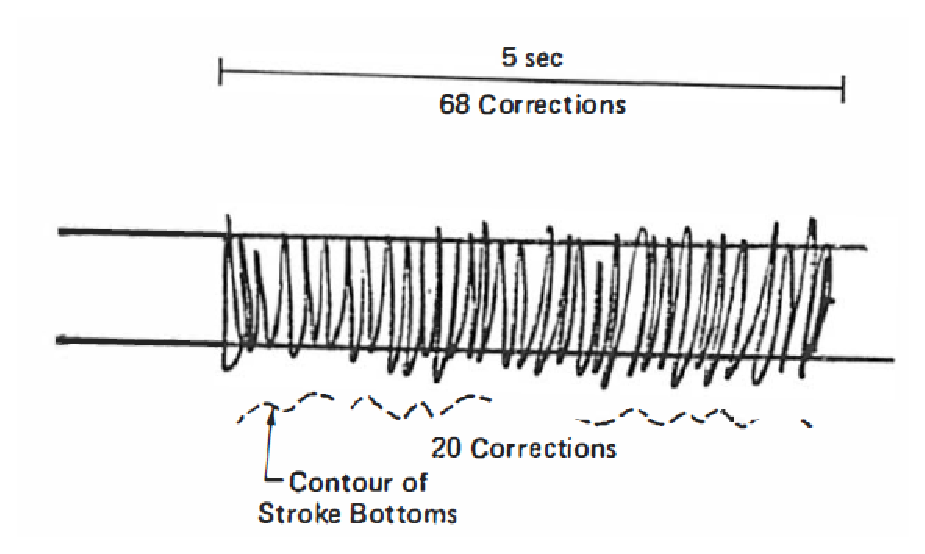
\includegraphics[width=0.5\hsize]{zigzag.eps}
 \end{center}
 \caption{ジグザグ運動の実験(図は[Wiley, 1978]のp.35より}
 \label{fig:zigzag}
\end{figure*}

一方、指の場合はキーボードを使った研究があり、
「同じキーを連続して打つ」という調査では、平均180[ms]/打(一回の運動あたり90[ms]; 押し上げと押し下げ)だそうです[Wiley, 1978]。
これは秒間打鍵に換算すると約5.6打/秒となります(あくまで同じキー連打の場合です)。

これを整理すると、表\ref{tbl:renzoku}のようになります。

\begin{table*}
\begin{center}
\caption{連続運動における所要時間}
\begin{tabular}{ccc}
\hline
鉛筆のジグザグ & 70[ms] (30~100[ms]) & 14回/秒 \\
腕・足・舌の繰り返し & 100[ms] & 10回/秒 \\
キーボード 同一キー連続 & 180[ms] & 5.6打/秒 \\
\hline
\end{tabular}
\label{tbl:renzoku}
\end{center}
\end{table*}

\subsubsection*{フィッツの法則}

以上のような知見を利用してモデルを立てることができます。
いま、距離$D$の場所に幅$S$(今は一次元の運動のみを考えます。
つまり、縦方向には無限に伸びているものとします)の物体があるとします。
この物体に腕・指を動かして触れる、というタスクを考えます(図\ref{fig:fitts})。

「目標物に対して腕・指を動かして触れる」という動作は一動作に見えますが、実はいくつもの離散的な運動の連鎖からなっています。
つまり、対象物との距離を計りながら少しずつ何度も何度もフィードバックさせ、減速や方向調整などをしています。

\begin{figure*}[htbp]
 \begin{center}
  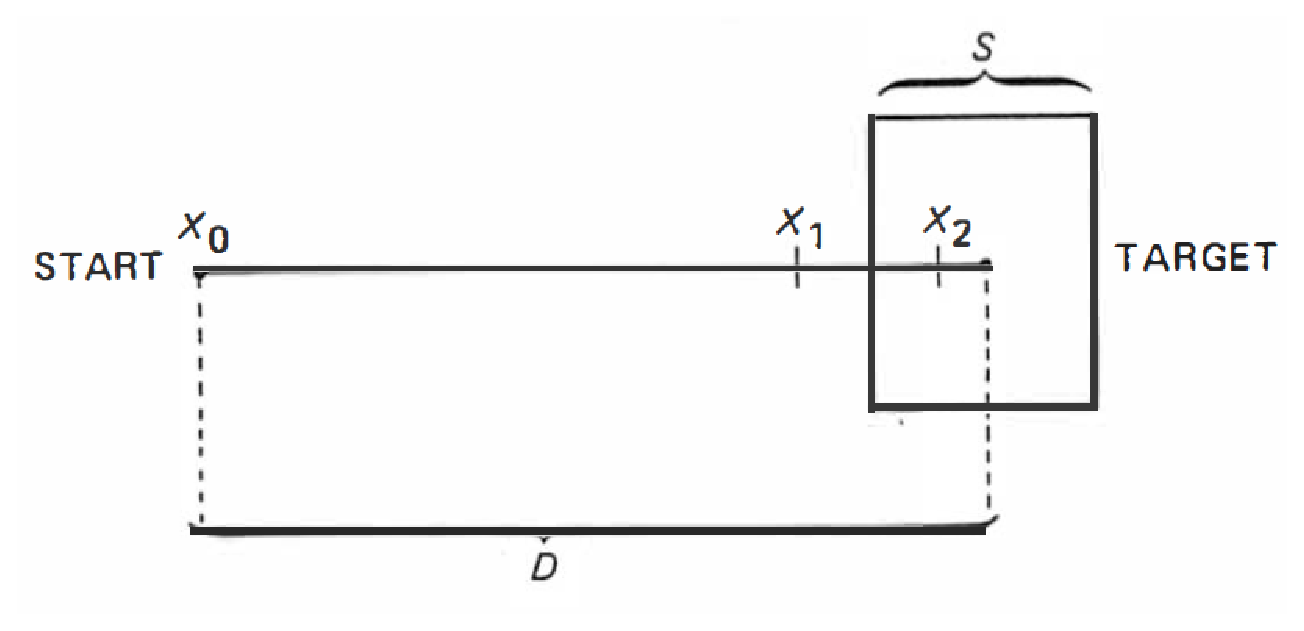
\includegraphics[width=0.5\hsize]{fitts.eps}
 \end{center}
 \caption{フィッツの実験}
 \label{fig:fitts}
\end{figure*}

ここからは専門的になるので導出はコラムに任せるとして、このタスクと所要時間$T$[ms]の間に、次のような法則が得られます:
\[
  T = I_M \log_2 \left(\frac{D}{S} + 0.5\right)
\]
ここで、$I_M$は100 [ms/bit]です\footnote{$\log$の中は無次元なので、一見無次元に見えますが、$\log$は底、つまり$\log_{e}$なのか$\log_{10}$なのかを区別するために、特別に単位をつけます。2を底とする場合は、bitをつけます。ちなみに前者$e$は\ruby{nat}{ナット}、$10$は\ruby{dit}{ディット}と言います。}%
(70~120)。

直感的には、こんな感じの説明になります。すごく遠いところにある(⇔$D$がとても大きい)と$T$は大きくなります。
一方、対象物がすごく大きい(⇔$S$がとても大きい)と、当然触れやすいので$T$は小さくなる、つまり速く押せます
(表\ref{tbl:fitts2})。

\begin{table}[htbp]
 \begin{center}
 \caption{フィッツの法則}
 \begin{tabular}{ccccc}
 \hline
  & {\bf\LARGE 近い} & $\cdots$ & {\bf\small 遠い} \\
  & \multicolumn{3}{c}{短時間 $\Longrightarrow$ 長時間} \\
  & {\bf\LARGE でかい} & $\cdots$ & {\bf\small 小さい} \\
 \hline
  \end{tabular}
  \label{tbl:fitts2}
\end{center}
\end{table}

%\begin{itembox}{{\bf コラム フィッツの法則の導出}}
\subsubsection{(発展:フィッツの法則の導出)}

\hspace{1zw}
「対象物との距離を計りながら動かす」離散的な動作を1サイクルと定義します。このとき、1サイクルごとに
\[
  T_{cycle} = T_p + T_C + T_M \simeq 240 {\mathrm ms}
\]
の時間がかかります。$T_p, T_C, T_M$は前に定義した値です。
$n$サイクルで対象物に到達するとすると、合計時間$T$は
\[
  T = n \cdot T_{cycle} = n ( T_P + T_C + T_M )
\]
となります。

ここで、$i$サイクル目での対象物への距離を$X_i$とします。$X_0 = D$です。1サイクルごとに制御する正確さは変わらないと仮定すると、
ある数$\epsilon < 1$を用いて$X_i = \epsilon X_{i-1}$と表すことができます({\bf 差}ではなく{\bf 比}を使うのがポイントです)。

すると、到達時の対象物への距離$X_n$(この時点でほとんどゼロに近くなっている)は
\[
X_n = \epsilon^n D
\]
と表せます。これが幅$S$に収まっていれば(=接触していれば)よいのですが、「行き過ぎ($+S/2$)」と「行き足りない($-S/2$)」があるので$1/2$します。つまり、
\[
  \epsilon^n D \le \frac{S}{2}
\]
これをnについて解くと、
\[
  n = -\log_2 (2D/S) / log_2 \epsilon
\]
この$n$を$T$の式に代入することによって、
\[
  T = I_M \log_2 (2D/S) \quad \mathrm{[ms]}
\]
を得ます。ただし、$I_M = -(T_P + T_C + T_M) / \log_2 \epsilon$です。

定数$\epsilon$はだいたい0.07とされています([Keele,1968][Vince,1948])。よって$I_M$は、
\begin{eqnarray*}
I_M &=& -240 / \log_2 (0.07) \\
    &=& 63 \quad \mathrm{[ms/bit]}
\end{eqnarray*}
となります。
\begin{flushright}
■
\end{flushright}
%\end{minipage}
%\end{itembox}

\subsubsection*{練習の効果 --- べき乗則}

さて、ここまでモデルを立てて計算してきたわけですが、人間はなにごとにも上達します。つまり、練習を重ねることによって、キーボードも速く打つことができます。

[Snoddy,1926]は、「ものを知覚してある運動をする時間」と練習量の間に次の関係を見出しました(Power Law of Practice)。
いわゆる{\bf 「べき乗則」(Power Law)}として知られている法則です。
\[
  n回目の試行における時間 T_n = T_1n^{-\alpha}
\]
ただし、$\alpha$はある定数です。

わかりやすくするために、$\alpha=1$としてみましょう。つまり、$T_n = T_1/n$です。この場合、2回目の試行で最初の試行の半分、3回目で三分の一、4回目で四分の一となります。グラフに表すと反比例のグラフになります。{\bf 最初のほうでぐっとタイムが縮まり、後のほうではタイムの縮まりは伸び悩んでいる}ことがわかりますね。

それをわかりやすく図示したのが、図\ref{fig:powerlaw}で、$y=1/\sqrt{x}\ (=1/x^{0.5}),\  y=1/x,\  y=1/x^2$のグラフです。上の式でいうと、それぞれ$\alpha = \frac{1}{2}$(実線)、$\alpha = 1$(破線), $\alpha = 2$(点線)の場合です。
$\alpha$が小さい(=実線になっていく)と、なかなかタイムが縮まりにくい(=縦軸が下がりにくい=タイムが縮まりにくい=上達しにくい)ことがわかりますね。

\begin{figure*}[htbp]
 \begin{center}
  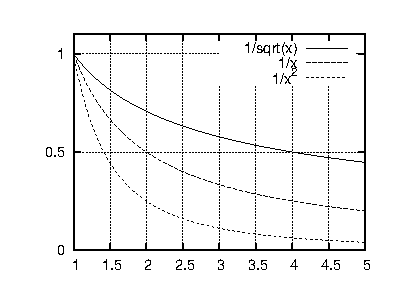
\includegraphics[width=0.7\hsize]{graph.eps}
 \end{center}
 \caption{べき乗則の例($y=1/\sqrt{x}$、$y=1/x$、$y=1/x^2$のグラフ)}
 \label{fig:powerlaw}
\end{figure*}

次に挙げる実験では、$\alpha = 0.38$という値が得られています。
(上で挙げた$1/\sqrt{x}$よりもさらに上達しにくい!)

詳しく説明しましょう。
図\ref{fig:powerlaw2}は[Klemmer,1962]による実験のグラフです。
Klemmerは、被験者に10個のボタン($2^{10} =1024$通り)のパターンを練習させました。

\begin{figure*}[htbp]
 \begin{center}
  \includegraphics[width=0.85\hsize]{powerlaw2.eps}
 \end{center}
 \caption{キー入力における べき乗則の実験(図は[Wiley, 1978]のp.59より}
 \label{fig:powerlaw2}
\end{figure*}

図\ref{fig:powerlaw2}を詳しく見てみましょう。両対数グラフになっているのでわかりにくいですが、たとえば{\bf 1000msから900msまで100ms縮めるのに1000回練習している}ことが、左から三番目と四番目の点からわかります。黒点はだいたい1000回ごとの練習を表しています。
また、$x$軸の10,000の右側、10000回目から20000回目の間に、点が密集しているのが見えますね。これは、{\bf 600msから500msまで100ms縮めるのに10000回もかかった}ということを表しています。1000ms→900msと比べて{\bf 10倍も練習量が必要}というのがわかります。

このように、ある$n$(ここでは練習回数)に対して、対応する関数$T(n)$(ここではタイム$T$)が$1/n$に比例することを、{\bf べき乗則}と言います。\footnote{余談ですが、自然界にはこのようにべき乗則が多く見られます。たとえば、ある文章中の単語を頻度順(多い順)に並べたときに、第$n$位の単語の文章中に占める割合は$1/n$にほぼ比例します({\bf Zipf(ジフ)の法則})。実際、theは文書中の7\%を占め、次にofがその半分の3.5\%を占めます。}

\subsubsection*{タイピング速度の理論と実際}

ここまで出てきた知識で、タイピング速度の理論値を計算してみましょう。

ものすごくざっくりと計算します。「鉛筆をひたすら速く上下させてジグザグ状に書く」という動作で測定した計測値$T_M = 30 \sim 100$[ms]を用います。キーを押すのには「押し下げ+押し上げ」の二動作がありますから、$2\times T_M$となります。
しかし、左右交互に押し下げ/押し上げを繰り返すので、結局のところ理論値は$T_M$となり、%
{\bf 秒間33打鍵~10打鍵(平均14打鍵/秒)}となります。実際には知覚による判断も入ってきますので、上限の33打鍵は不可能でしょう。

実際のところどのくらいまで速くなるのでしょうか?

表\ref{tbl:speed}に、タイプライタでの一ストロークあたりの時間を挙げます\footnote{おまけで他にも載せました。表の値は[Wiley, 1978]によります。}。文献による{\bf タイピングチャンピオンは60[ms/打]で、これは16.7[打/秒]に相当します}。タイプウェル国語Rや英単語(400打鍵)だと{\bf 24秒}で打ちきることができる試算になります。

\begin{table*}[htbp]
 \begin{center}
     \caption{タイプライタにおける打鍵速度}
 \begin{tabular}{lcc}
\hline
タイプライタ & [ms/打] & 秒間打鍵数[打/秒] \\
\hline
Best case(チャンピオン) & 60 & 16.7 \\
テキストタイピング & 158~231 & 4.3~6.3 \\
テキストタイピング(ランダム単語列) & 200~273 & 3.7~5 \\
テキストタイピング(ランダム文字列) & 462~500 & 2~2.2 \\
アルファベット手書き & 545~932(ms/字)  & 1.1~1.8 \\
\hline
 \end{tabular}
 \label{tbl:speed}
 \end{center}
\end{table*}

\subsubsection{各キーごとの実測}

キーボード入力の速さを、もう少し詳しく見た研究があります。図\ref{fig:kinkead1}はQWERTYキーボードにおける各キーの、
\begin{itemize}
 \item 同手打鍵
 \item 異手打鍵
 \item 同指打鍵
 \item 同キー連続
\end{itemize}
の四種類それぞれの条件下で打ったときにかかる時間を示しています[Kinkead,1975]。

例として一つ見てみましょう。図\ref{fig:kinkead_k}にKのキーを載せます。
左上の数値162は、同じ右手でキーを打ったとき、たとえば\key{O}\key{K}を打ったときに\key{K}を打つのにかかる時間を表しています。
同様に、右上の数値133は、左手で前のキーを打ったとき、例えば\key{C}\key{K}を打ったときに\key{K}を打つのにかかる時間を表しています
({\bf 同手打鍵よりも交互打鍵のほうが速い}、ということも見てとれますね)。

\begin{figure*}[tbp]
 \begin{center}
  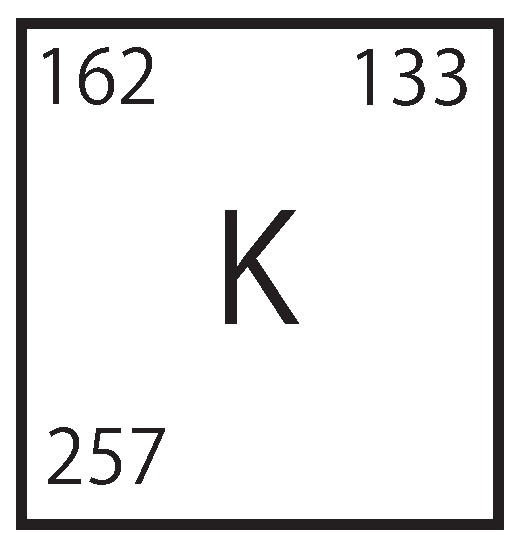
\includegraphics[width=0.15\hsize]{kinkead2.eps}
 \end{center}
 \caption{Kinkeadによるキー入力間の打鍵時間、Kの例}
 \label{fig:kinkead_k}
\end{figure*}

\begin{figure*}[htbp]
 \begin{center}
  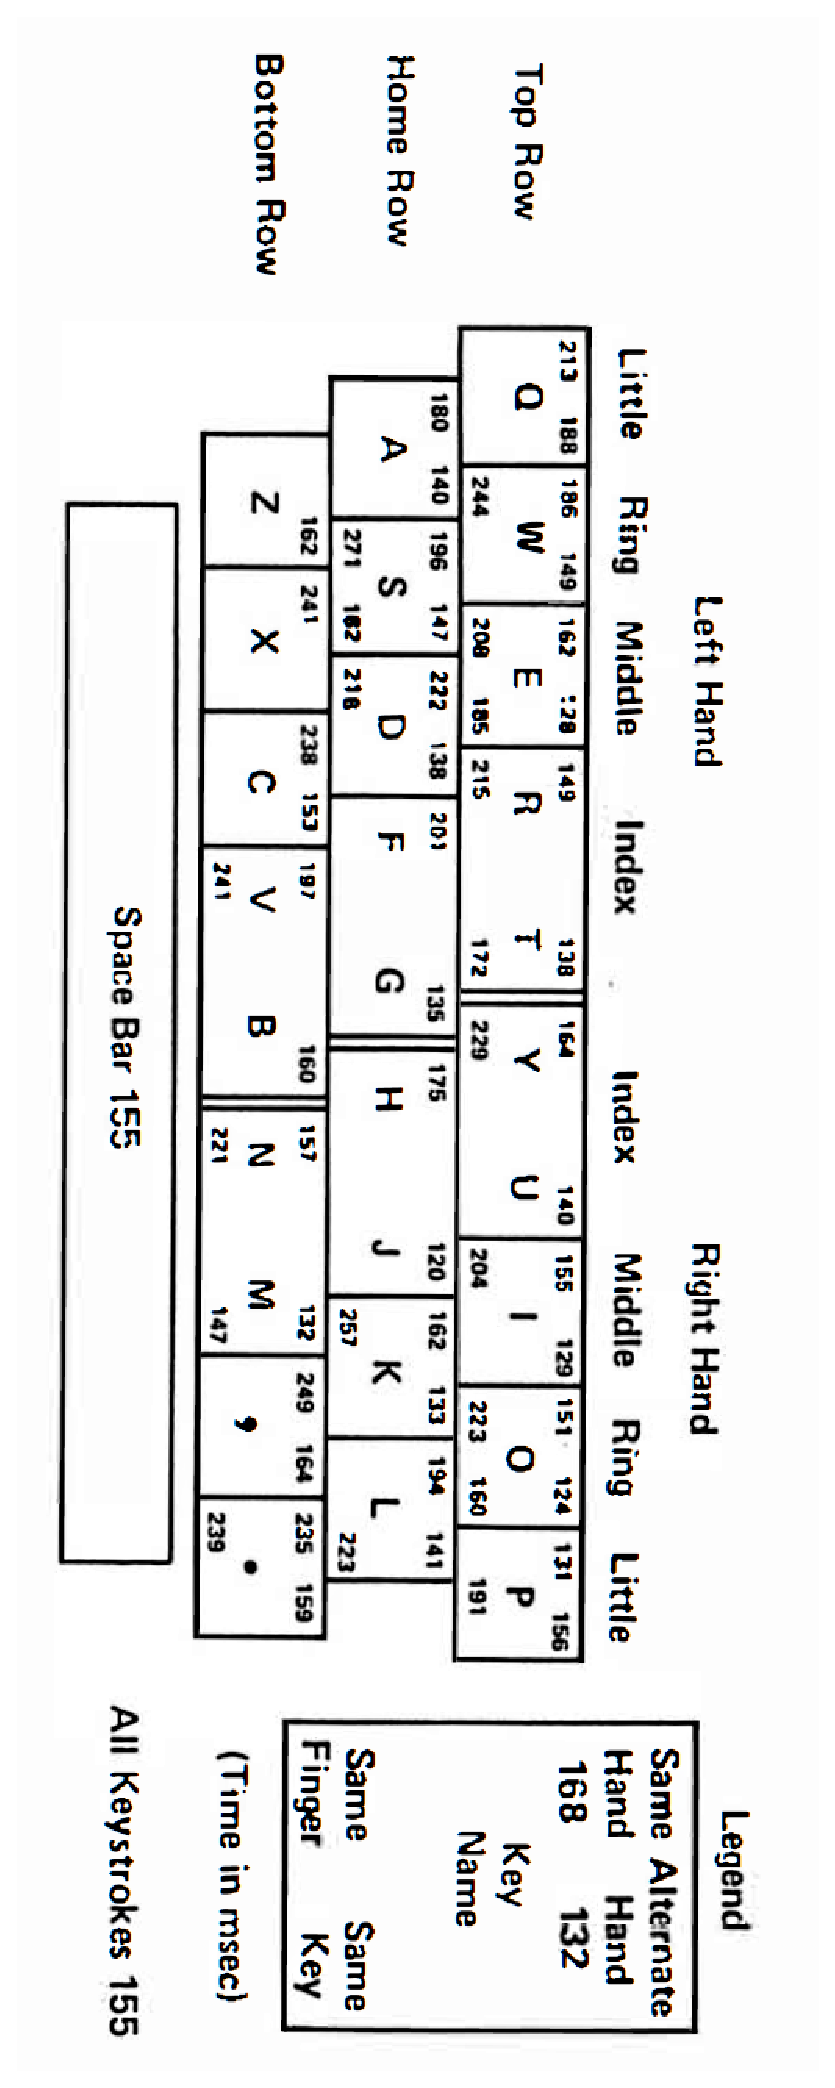
\includegraphics[height=0.9\vsize]{kinkead.eps}
 \end{center}
 \caption{Kinkeadによるキー入力間の打鍵時間(図は[Wiley, 1978]のp.62より}
 \label{fig:kinkead1}
\end{figure*}

Kinkead(1975) は図\ref{fig:kinkead1}の表の数値と、実際の英語の文字の出現頻度を用いて、タイピング時間を推計しました。
具体的には、2文字の連接(bigram)の頻度を用いて、
\[
  \mathrm{Typing rate} = \sum_i f_i t_i
\]
と計算しました。ただし、$f_i$はbigramの出現頻度、$t_i$はbigramに対応する図\ref{fig:kinkead1}の数値です。
この計算により、KinkeadはQWERTYのタイピング速度を162ms/打と推定しました。秒間打鍵に換算すると6.2打/秒となります。
Kinkeadは同じ計算をDvorakについても行い、QWERTYに比べて2.6\%しか速くなっていないということを示しました。

タイピング速度のシミュレーションを、このようなbigramの入力速度の総和で近似するという手法は、古典的ですが配列設計の最適化に役立つと言えましょう\footnote{ただし、Kinkeadのシミュレーション結果は「悪運指は良運指に悪影響を及ぼさない」という仮定をおいています。これは[Yamada, 1980a][Yamada, 1980b]の実験によって否定されています。今回は時間がなかったのでまた次回。}。

\section{配列解析編}

\subsection{はじめに}

この章では、世の中に存在する種々の配列のうちいくつかをピックアップして、それらについて定量的な分析を試みます。
具体的には「総打鍵数」「総打鍵数のうち、左・右の数・割合」「シフト数」「左手・右手の各指における使用数・比率」を見ます。
各段における使用比率も見ます。これは主として、ホームポジションから手が離れにくいかどうかを見る指標となります。
また、打ちやすさにおいて重要な因子となる、「連続して同じ指を使って打つ(同指異鍵; KIKIなど)」
「同じ手で段を二段以上飛び越えて打つ(同手跳躍; MIMIなど)」
「左手の縦の連続(左手縦連; WAZAWAZAなど)」も数えます。

以下にQWERTYローマ字入力を例にとって見てみましょう(表\ref{tbl:roma_example})。

まず一段目が、総打鍵数と、左手・右手での打鍵数とその比率です。シフト数はシフトを押した回数で、括弧内はクロスシフトです(NICOLA配列、中指シフト配列で効いてきます)。右側の「交互/左左/右右」は、二文字間での手の動きを示したものです。
二段目は各指の使用比率となっています。左から左小指、薬指、……、右小指となっています。
三段目は先行研究で議論されている「同じ指で違うキーを連続で打つ(同指異鍵)」「同じ手で段を二段以上飛び越えるキーを打つ(同手跳躍)」「左手で連続した縦のキーを打つ(左手縦連; \key{Z}\key{A}など)」の使用数、および各段ごとの使用比率となっています。


\begin{table*}[htbp]
 \caption{QWERTYローマ字の解析表}
 \begin{center}
 \begin{tabular}{cccc|ccc}
 \hline
総打鍵 & 総打鍵左 & 総打鍵右 & シフト数 & 交互 & 左左 & 右右 \\
37818164 & 16102479 & 21715685 & 7216(7216) & 17753448 & 7225755 & 12838961 \\
 & 42.6\% & 57.4\% & & 46.9\% & 19.1\% & 33.9\% \\
 \hline
 \end{tabular}

  \vspace{1zw} 

 \begin{tabular}{ccccccccccc}
 \hline
& 左小(A) & 左薬(S) & 左中(D) & 左人(FG) & 右人(HJ) & 右中(K) & 右薬(L) & 右小(;)\\
& 5180235 & 2405277 & 3120281 & 5396686 & 9531741 & 7001152 & 4679026 & 503766\\
左/右手中 & 32.2\% & 14.9\% & 19.4\% & 33.5\% & 43.9\% & 32.2\% & 21.5\% & 2.3\%\\
総打鍵中 & 13.7\% & 6.4\% & 8.3\% & 14.3\% & 25.2\% & 18.5\% & 12.4\% & 1.3\%\\
\hline
 \end{tabular}

  \vspace{1zw} 

 \begin{tabular}{ccc|cccc}
 \hline
 同指異鍵 & 同手跳躍 & 左手縦 & 最下段(ZX..) & ホーム(AS..) & 三段目(QW..) & 最上段(12..)\\
 2991366 & 5170649 & 3457 & 6024198 & 12333179 & 19265593 & 195194\\
  &  &  & 15.9\% & 32.6\% & 50.9\% & 0.5\%\\
%交互/左左/右右 中 & 交互/左左/右右 中 & 交互/左左/右右 中 &  &  &  & 総打鍵中 & 総打鍵中 & 総打鍵中 & 総打鍵中\\
\hline
 \end{tabular}
 \end{center}
 \label{tbl:roma_example}
\end{table*}

\subsection{QWERTYについて}

まず(個性的な)各配列に移る前に、研究が進んでいるQWERTYについて見てみることにします。その後、AZIK、かな配列と見ていきます。

\subsubsection*{QWERTYは「打ちやすい」か?}

みなさんがいちばん目にすることの多い配列、QWERTYはタイプライターの配列に始まります。1868年にはアルファベットをそのまま並べたものであったタイプライターの配列が、現在のQWERTY配列と同じものになったのは、1882年8月のことです(安岡孝一ら『キーボード配列QWERTYの謎』、NTT出版、2008年)。

QWERTYキーボードに対する批判は数多くあり、またそれらが他の配列を考案させる動機にもなっています。
(1983年当時の)過去50年間におけるQWERTY配列に対する批判をまとめると%
%\footnote{主としてDvorak博士とそのチームによる批判でした[Dvorak, 1943]。DvorakらのQWERTY配列批判は熾烈で、FIXME}%
[Noyes, 1983]、

\begin{enumerate}
\item 左手に過負荷である。キーの実行の57\%が、多くの人が利き腕でない左手により行われる%
    \footnote{これは英語の場合であることに注意してください。日本語の場合はこれと異なります。詳しくは後述のローマ字入力で。}
\item ある指にとって過負荷である\footnote{機械式のタイプライタでは、全ての指で同じ力を使って入力する必要がありました。そのため、小指や薬指など、力の弱い指に負担がかかることがあったようです。電動式になってから、この欠点はさほど問題ではなくなりました。}
\item 中段のキーの実行が少なすぎ(32\%)、上段のキーの実行が多すぎる(52\%)
\item よく使用される単語において、段の変更が多すぎる。しばしば下段、上段、下段となることがある。たとえば ``br, un, in''など。
\item 多くの一般用語が左手だけでタイプされる。たとえば ``was, were, extra, address''
\end{enumerate}

このうち3番目は補足が必要です。[Kinkead, 1975]によると、機械式のタイプライタでは中段のキーをおすのが最も速く、電気的なタイプライターでは上段のキー操作が最も速いと論じています(熟練したタイピストによる実験)。

\subsection{QWERTYローマ字入力}

さて、ここからは日本語タイピングについて議論していくことにします。
まずは、おそらく一番標準的な入力方式であるローマ字入力から。

QWERTYローマ字入力をコーパスを用いて評価すると表\ref{tbl:roma_example}のようになります。

日本語のタイピングにおいては、前述のNoyesの主張(左手偏重)に対して、
右手偏重の配列になっていることがうかがえます。
特に、右手人差し指の使用率が他の配列と比べ高くなっています。

この、右手偏重・右手人差し指偏重の結果については、次の点が原因として考えられます。
\begin{itemize}
\item 日本語は「子音+母音」で一文字となるがそのうち右手で打つ母音(\key{I}\key{O}\key{U})が母音中の約6割を占め、左手に比べてやや多いこと、
\item よく出る仮名の子音が、右手人差し指に集中していること、
\item[ ] \hspace{1zw}(頻度順に挙げると、「%
{\footnotesize い}%
\ruby{{\bf う}}{U}%
\ruby{{\bf ん}}{N}%
{\footnotesize し}%
\ruby{{\bf の}}{N}%
{\footnotesize かたと}%
\ruby{{\bf に}}{N}%
{\footnotesize て}%
\ruby{{\bf な}}{N}%
\ruby{{\bf は}}{H}」の太字)。
\end{itemize}

一方、左手の方は左小指の酷使がひどく、他の配列に比べ群を抜いています。「\ruby{笹}{ささ}沢(SASAZAWA)」などの「沢」が付く人名や、「わざわざ(WAZAWAZA)」の打ちにくさは、多くの人が経験していることと思います。

%\begin{table}[htbp]
% \begin{center}
%  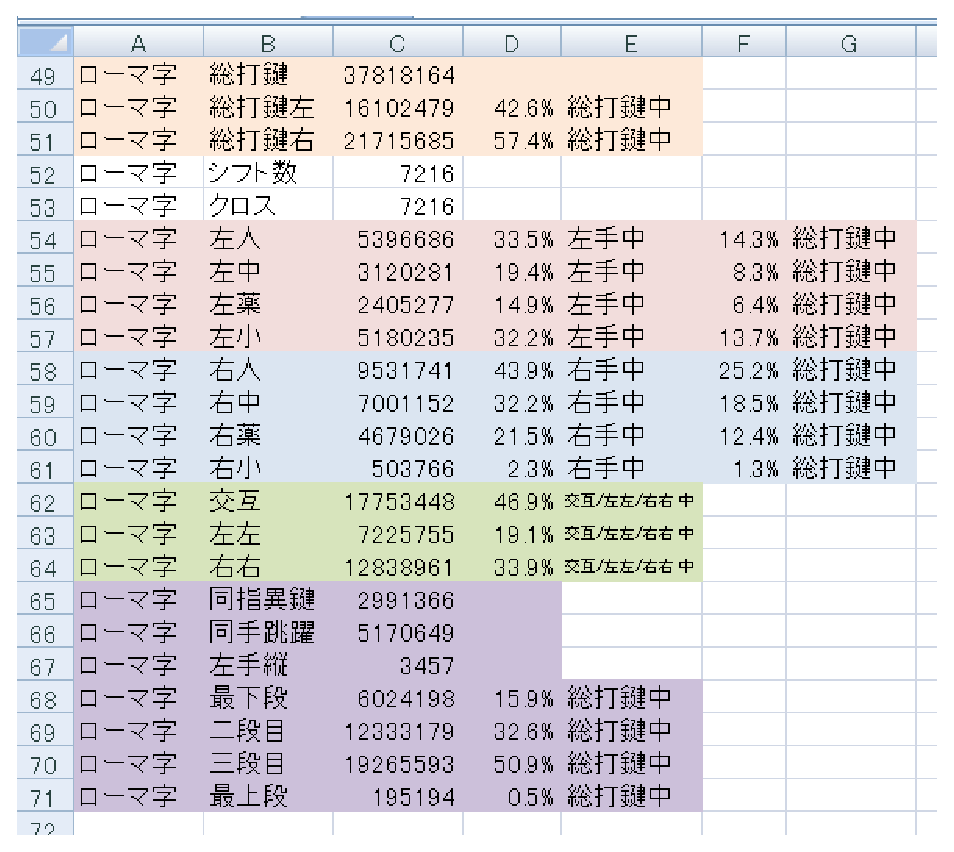
\includegraphics[width=0.85\hsize]{tbl-roma.eps}
% \end{center}
% \caption{QWERTYローマ字の解析表}
% \label{tbl:roma}
%\end{table}

\subsection{AZIK}

QWERTYによるローマ字入力を少し改良したのが、AZIKです。
AZIKでは、日本語の漢字の音の多くが「い」「ん」「う」
(「\ruby{会}{かい}」「\ruby{完}{かん}」「\ruby{項}{こう}」など)で終わることに着目しました。
より正確に言えば、ローマ字で書いて、-ai、-an、-ouなどの音で終わる文字が多い、ということです。
そこでAZIKでは、この``ai''、``an''に、一文字を割り当てることにしました。
たとえば``ai''は\key{Q}、``an''は\key{Z}です。日本語では、子音と母音が交互に連なることから「子音+子音」の組み合わせになったとき(たとえば``KZ'')のみ
\key{Z}をanと解釈すれば、「ざじずぜぞ」と競合することはありません%
\footnote{これは、ATOKやGoogle日本語入力のローマ字変換テーブルで容易に実装できます。}。%
日本語の漢字は全文章の約3割を占めますので、これらの漢字音の入力を省入力化すれば、全体的な打鍵数は少なくなります。

また、AZIKでは「っ」の文字を一文字(\key{;})で入力したり、頻出の「する」「こと」などを``sr''、``kt''で入力するなど、随所に省入力化が見られます。

その他特筆すべきこととして、きゃ行、ひゃ行、みゃ行などの\ruby{拗}{よう}音について、``KYU''などではなく``KGU''でも打てるようにしている点があります。これは省入力化ではなく、左右交互打鍵を狙った改良です。このような交互打鍵を目的とした拡張として、「だん」(DZ)を``DN''でも打てるようにしたものもあります。

さて、AZIKをコーパスを使って評価してみましょう。
%AZIKについては、作者が省入力化に段階を設けていますので、二種類の評価設定をとりました。具体的には、「AZIK総合解説書\footnote{{\tt http://hp.vector.co.jp/authors/VA002116/azik/azikinfo.htm}}」にある「その2(拡張キー)」のみのと、「その3」まで全て使用した場合の二通りです。
評価には、
\begin{itemize}
 \item \ruby{撥}{はつ}音拡張(-anなど, キー:ZNKJDL)(\key{Z}と\key{N}については、前節で述べた交互打鍵の優位性を\ruby{鑑}{かんが}みて、交互打鍵になるように各キーを選択しました)
 \item 二重母音拡張(-aiなど、キー:QHWP)
 \item 「し」「しょう」などshの音を\key{x}で入力 / 「ち」などchの音を\key{c}で入力
 \item 「ん」「っ」をそれぞれ\key{Q}, \key{;}で入力
 \item \ruby{拗}{よう}音を\key{Y}ではなく\key{G}で入力
 \item 「する」「こと」などをそれぞれ\key{S}\key{R}、\key{K}\key{T}などで入力
\end{itemize}
という設定を用いました。これは「AZIK総合解説書\footnote{\url{http://hp.vector.co.jp/authors/VA002116/azik/azikinfo.htm}}」にある、「その3」までの設定をほぼ踏襲しています。

%\begin{table}[htbp]
% \begin{center}
%  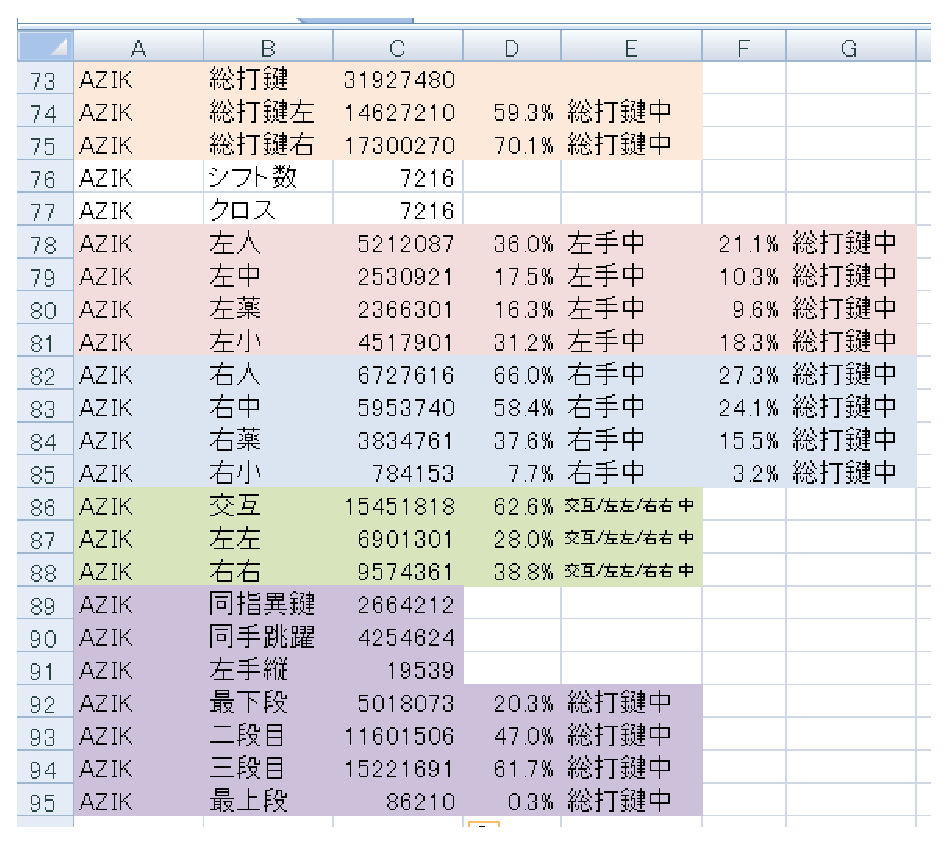
\includegraphics[width=0.85\hsize]{tbl-azik.eps}
% \end{center}
% \caption{AZIKの解析表}
% \label{tbl:azik}
%\end{table}

\begin{table*}[htbp]
 \caption{AZIKの解析表}
 \begin{center}
 \begin{tabular}{cccc|ccc}
 \hline
総打鍵 & 総打鍵左 & 総打鍵右 & シフト数(クロス) & 交互 & 左左 & 右右 \\
30200816 & 14072150 & 16128666 & 98014(9948) & 15211220 & 6466540 & 8523056 \\
 & 46.6\% & 53.4\% &  & 50.4\% & 21.4\% & 28.2\% \\
 \hline
 \end{tabular}

  \vspace{1zw} 

 \begin{tabular}{ccccccccccc}
 \hline
& 左小 & 左薬 & 左中 & 左人 & 右人 & 右中 & 右薬 & 右小 \\
& 3998593 & 2366304 & 2145980 & 5561273 & 6426213 & 5422220 & 3496080 & 784153 \\
左/右手中 & 28.4\% & 16.8\% & 15.2\% & 39.5\% & 39.8\% & 33.6\% & 21.7\% & 4.9\% \\
総打鍵中 & 13.2\% & 7.8\% & 7.1\% & 18.4\% & 21.3\% & 18.0\% & 11.6\% & 2.6\% \\
\hline
 \end{tabular}

  \vspace{1zw} 

 \begin{tabular}{ccc|cccc}
 \hline
 同指異鍵 & 同手跳躍 & 左手縦 & 最下段(ZX..) & ホーム(AS..) & 三段目(QW..) & 最上段(12..)\\
2030767 & 3797767 & 15170 & 5018292 & 11429889 & 13666425 & 86210 \\
 &  &  & 16.6\% & 37.8\% & 45.3\% & 0.3\% \\
%交互/左左/右右 中 & 交互/左左/右右 中 & 交互/左左/右右 中 &  &  &  & 総打鍵中 & 総打鍵中 & 総打鍵中 & 総打鍵中\\
\hline
 \end{tabular}
 \end{center}
 \label{tbl:azik}
\end{table*}

さてAZIKは、QWERTYローマ字(約3782万字)に比べ、約20\%打鍵数を削減できています。これは前述の二重母音などの省入力に加え、日本語で頻出の「する」「こと」を2ストロークで入力できるようにしたことも大きいのでしょう%
\footnote{ちなみに2000万字のコーパスでは、「する」は57752回、「こと」は88757回出ていました。}。

左手の子音のキーを多用することから、左手の使用率は若干高くなりました。
しかし、\key{Q}/\key{Z}を打つべき左手小指については、ローマ字の13.7\%に比べてAZIKが13.2\%と、ほとんど変わっていません。

AZIKの配置は覚えやすさのために、対応する母音のキーの近く(-ai/-anなら\key{A}の近くの\key{Q}と\key{Z})
という条件を設けていました。そのため、キーボード配列の打ちやすさという観点から言えばむしろ、
不利なものとなってしまう危険性を持っています。

実際、上で述べたような工夫を使わず、単純な\ruby{撥}{はつ}音拡張(ZKJDL)、二重母音拡張(QHWP)だけを使った
予備実験では、\key{A}と\key{E}が左手にあること、\key{Q}と\key{Z}が左手小指であることに引きづられて、
左手小指・薬指を酷使する配列になってしまっていました。

AZIKは、省入力化の方法をふんだんに用い、さらに交互打鍵まで考慮した結果として、
覚えやすさと効率を両方カバーした、バランスのとれた配列になった、と言えるでしょう%
\footnote{ただし、``sr''→する、以外の比較的頻度の低い二文字が覚えやすいかどうかは議論の余地があります。}。

%原理上、``ai''などのキーはどの子音のキーに置いてもよいため、これについては改良が望めます%
%\footnote{そのため、筆者(nooyosh)はいまYAZIK: Yet another AZIKという配列を考えているので、次回以降乞うご期待。}。

\subsection{JISかな}

みなさんご存じの「たていすかんなにらせ」――JISかな%
\footnote{次に説明する「新JIS配列」との比較で「旧JIS」と呼ばれることもあります。}%
は、当初カナタイプライタの配列から考案され、1972年にJISC 6233として制定されました。特徴としては、(ほぼ)すべてのキー使って仮名を配置しようとしたために、キーを四段すべて使っている点です。
後述する親指シフトや中指シフトなどのように、シフトキーを押す必要がないために直感的ではあるのですが、
\begin{itemize}
\item 上から二段目の使用頻度が高く、ホームポジションから指が離れやすい
\item 打鍵が左手に偏っている
\item 数字を打つときにカナキーを押す必要がある
\end{itemize}
など、いろいろと欠点があります。

詳しく見てみましょう(表\ref{tbl:jiskana})

\begin{table*}[htbp]
 \caption{JISかなの解析表}
 \begin{center}
 \begin{tabular}{cccc|ccc}
 \hline
総打鍵 & 総打鍵左 & 総打鍵右 & シフト数 & 交互 & 左左 & 右右 \\
24675899 & 14475950 & 10199949 & 2666111(2213255) & 11525084 & 8713408 & 4437407\\
 & 58.7\% & 41.3\% &  & 46.7\% & 35.3\% & 18.0\%\\
 \hline
 \end{tabular}

  \vspace{1zw} 

 \begin{tabular}{ccccccccccc}
 \hline
& 左小(A) & 左薬(S) & 左中(D) & 左人(FG) & 右人(HJ) & 右中(K) & 右薬(L) & 右小(;)\\
& 5609655 & 3528341 & 2956460 & 2381494 & 3483694 & 2418311 & 2048886 & 2249058\\
左/右手中 & 38.8\% & 24.4\% & 20.4\% & 16.5\% & 34.2\% & 23.7\% & 20.1\% & 22.0\%\\
総打鍵中 & 22.7\% & 14.3\% & 12.0\% & 9.7\% & 14.1\% & 9.8\% & 8.3\% & 9.1\%\\
\hline
 \end{tabular}

  \vspace{1zw} 

 \begin{tabular}{ccc|cccc}
 \hline
 同指異鍵 & 同手跳躍 & 左手縦 & 最下段(ZX..) & ホーム(AS..) & 三段目(QW..) & 最上段(12..)\\
4885493 & 3477500 & 487390 & 4477353 & 6071650 & 10022415 & 4104481\\
 &  &  & 18.1\% & 24.6\% & 40.6\% & 16.6\%\\
\hline
 \end{tabular}
 \end{center}
 \label{tbl:jiskana}
\end{table*}

%\begin{table}[htbp]
% \begin{center}
%  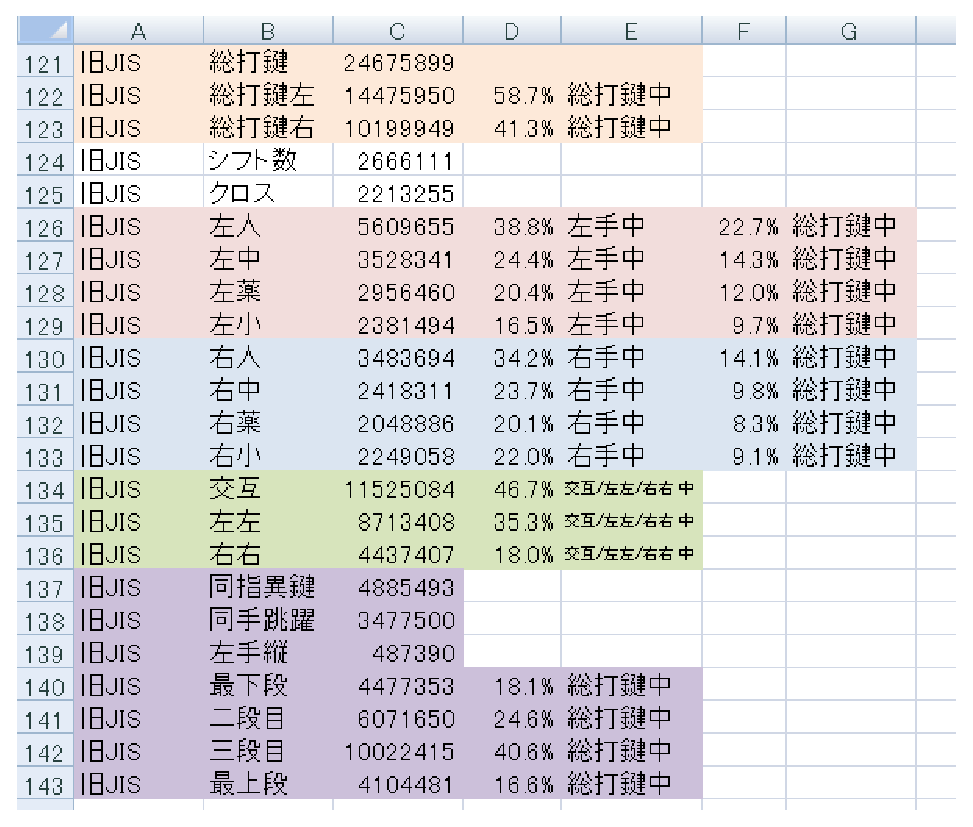
\includegraphics[width=0.85\hsize]{tbl-jiskana.eps}
% \end{center}
% \caption{旧JISの解析表}
% \label{tbl:jiskana}
%\end{table}

総打鍵中約6割が左手になります。そのうち、左人差し指が総打鍵の約23\%を占めるなど、著しい偏りが見られます(「う」「か」などが左人差し指の高頻度文字)。
bigram、つまり二文字列の連なりを見ても、左手→左手の組み合わせが4割弱と、左手の酷使が見て取れます(「てい」「った」など)。
また、上から二段目(QWE...)が総打鍵の約4割を占めるなど、ホームポジションから指が離れやすい点も確認できます。

\subsection{新JIS系・中指シフト系カナ配列}
\subsubsection*{新JIS}

JISかなの欠点を解消するため、1986年に新しい仮名配列がJISで決定されました。
これは、「頻度の比較的低いキーはシフトで入力させ、指がホームポジションからなるべく離れないようにする」という設計思想に基づいて考案された配列です。
一般に新JISと呼ばれます。
しかし、JISかなが廃止されずに併存したことから、新JISは全く普及せず、「使用実態がない」として1999年に廃止されてしまいました。

新JISの設計では、キーボード最上段(数字キーのある段)の入力スピードが、他の段に比べて遅いことに注目しました。
ホームポジションから遠いキーの入力が遅いことは、前述のフィッツの法則(遠くにある小さいキーほど入力速度が遅い)からもわかります。
そこで、新JISでは仮名をすべて三段に収めようとしました。三段では足りないので、出現頻度の低い文字についてはシフトキーを用いて入力するようにしました(「裏に配置」)。

次に、どう仮名を配置するかです。まず考慮されるべきは、出現頻度です。これに関しては、高校教科書の文章の「1文字の出現頻度」(unigramの頻度)、「2文字の連接の出現頻度」(bigramの頻度)が用いられました。

具体的には、次の1.から4.のステップを経ます。

\begin{enumerate}
\item 「1文字の出現頻度」が高い順(「い」「う」「ん」……)に仮名を並べ、半数を「シフトしないで入力されるキー」(「表」; アンシフト)に設定します。
例えば、「い」は日本語の文章で一番多く出現するため、当然表に出てきます。
\item これらを、交互打鍵率が最大になるように左右に分けました。「交互」の計算には、上であげたbigramを用います。これも上であげた「2文字の連接」(bigram)を使います。
    「てい」はとても多く(bigram全体の約0.7\%)見られるので、\key{て}と\key{い}のキーは(なるべく)左右に分離して配置した方がよいことになります。
\item 左右グループそれぞれについて、指の段越えが少なくなるような組み合わせを探します。
\item さらに、左右グループそれぞれについて、同じ指が連続して打つ(同指異鍵)回数が少なくなるような組み合わせを探します。
\end{enumerate}

シフトされる仮名の集合については、シフトキーを1ストロークと見なして、交互打鍵の頻度が最大になるように左右グループにわけ、さらにホームポジションの段に頻度の高い仮名を配列するようにしました。

これもコーパスを使って見てみましょう(表\ref{tbl:newjis})

\begin{table*}[htbp]
 \caption{新JISの解析表}
 \begin{center}
 \begin{tabular}{cccc|ccc}
 \hline
総打鍵 & 総打鍵左 & 総打鍵右 & シフト数 & 交互 & 左左 & 右右 \\
24706219 & 11010567 & 13695652 & 4031578\\
 & 44.6\% & 55.4\% & \\
 \hline
 \end{tabular}

  \vspace{1zw} 

 \begin{tabular}{ccccccccccc}
 \hline
& 左小(A) & 左薬(S) & 左中(D) & 左人(FG) & 右人(HJ) & 右中(K) & 右薬(L) & 右小(;)\\
& 4738263 & 2648262 & 2256137 & 1367905 & 5212719 & 3530762 & 3702200 & 1249971\\
左/右手中 & 43.0\% & 24.1\% & 20.5\% & 12.4\% & 38.1\% & 25.8\% & 27.0\% & 9.1\%\\
総打鍵中 & 19.2\% & 10.7\% & 9.1\% & 5.5\% & 21.1\% & 14.3\% & 15.0\% & 5.1\%\\
\hline
 \end{tabular}

  \vspace{1zw} 

 \begin{tabular}{ccc|cccc}
 \hline
 同指異鍵 & 同手跳躍 & 左手縦 & 最下段(ZX..) & ホーム(AS..) & 三段目(QW..) & 最上段(12..)\\
2495822 & 830701 & 38977 & 4876067 & 13254518 & 6496686 & 78948\\
 &  &  & 19.7\% & 53.6\% & 26.3\% & 0.3\%\\
\hline
 \end{tabular}
 \end{center}
 \label{tbl:newjis}
\end{table*}



%\begin{table}[htbp]
% \begin{center}
%  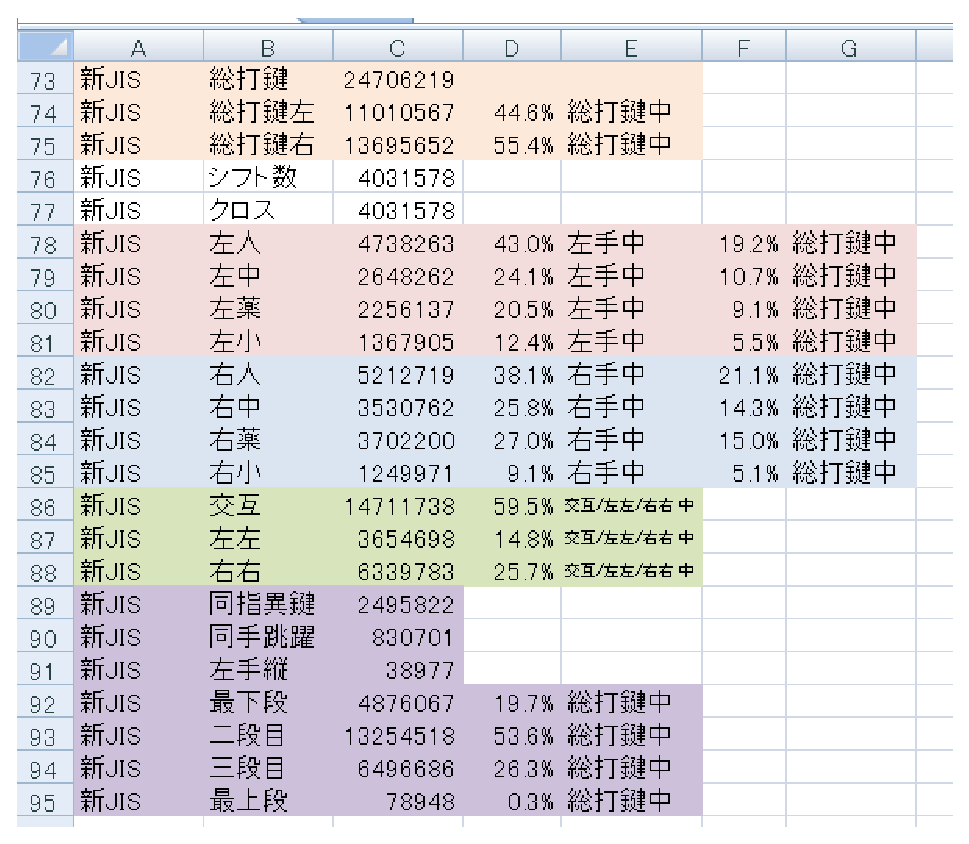
\includegraphics[width=0.85\hsize]{tbl-newjis.eps}
% \end{center}
% \caption{新JISの解析表}
% \label{tbl:newjis}
%\end{table}

右手と左手の\ruby{乖離}{かいり}が若干改善されました。また、交互打鍵が全体の約6割と、JISかなの約46\%と比べて大幅に改善されたことがわかります。
また、JISかなで38\%あった「左左」が15\%と、劇的に少なくなっています。上から三段目(ホームポジション)での打鍵が約54\%と、あまり指がホームポジションから離れないということも示唆されます。

\subsubsection*{花配列}

花配列は、冨樫雅文氏によって考案された、中指シフトと呼ばれる新しい配列です(図\ref{fig:hana}%
\footnote{図は「花のくに」\url{http://homepage3.nifty.com/togasi/hana_no_kuni/index.html} より。}%
)。新JIS配列では、仮名をホームポジション近くに収めるために、
シフトキーを用いていました。シフトキーはキーボードの右端と左端に置かれていますので、このままでは小指を酷使してしまいます。

そこで、冨樫氏は新しいシフト方式を考案しました。シフトキーを中指、QWERTYでいうDとKの位置に置き、しかもシフトを押すといったんロックされ、次の入力とともに解除される方式をとりました。
冨樫氏のこの方式は、中指シフト配列という新たな配列の分野を切り開いた、画期的な配列であると言えるでしょう。

さて、花配列では、「最もよい配列」を次のように定義しました。

\begin{itemize}
\item 1文字あたりの平均入力速度が最も速い
\item 各指にかかる負荷があらかじめ指定したものに最も近い
\end{itemize}

これらを定量的に明らかにするために、
\begin{itemize}
\item 仮名文字の使用頻度
\item 打鍵速度(打鍵間の所要時間)
\item 指の使用頻度分布
\end{itemize}
が使われました。
実際の配列設計では、まずランダムに配列を決定し、少しずつ(上の基準をみたすように)変化させていき、変化しなくなるまで10000回行いました。
これは、いわゆる焼きなまし法(Simulated Annealing)を行なっていたと考えられます。

ではコーパスを使ってみてみましょう\footnote{%
なお、シフトについては全てクロスシフトになるように(有利に)評価しました。
これについては評価がわかれる(アルペジオなど)ところですが、交互打鍵が最速という先行研究にしたがい、
クロスシフトを採用しました。以下の月配列などについても同様の設定です。}(表\ref{tbl:hana})。
%\begin{table}[htbp]
% \begin{center}
%  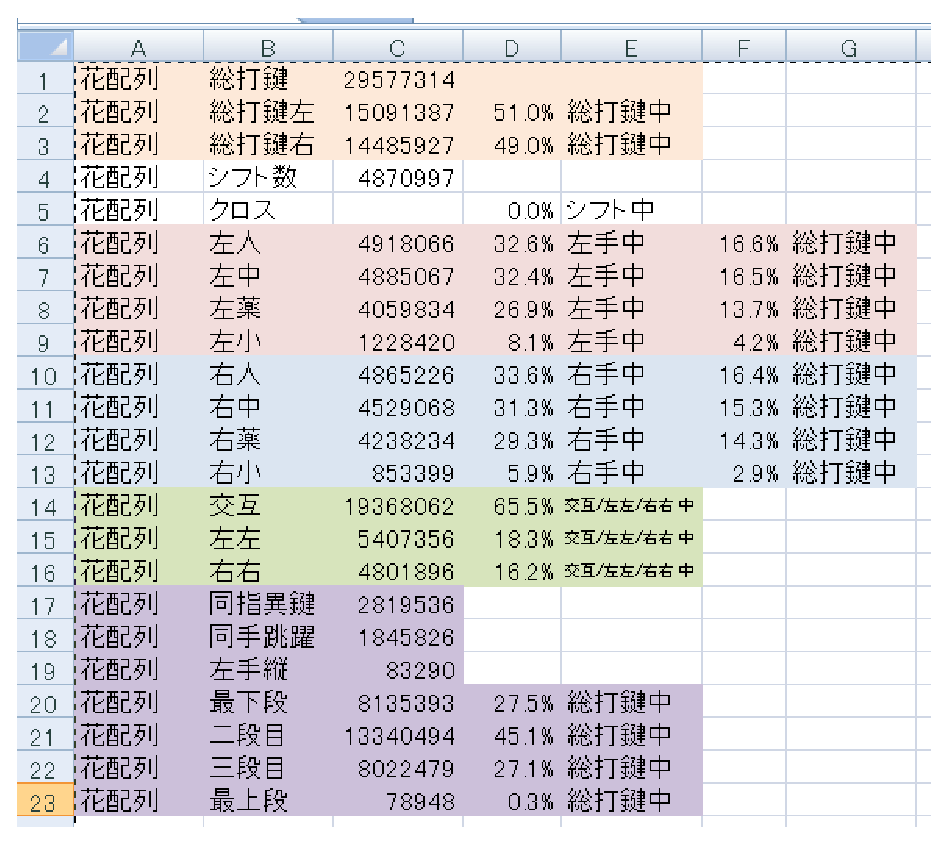
\includegraphics[width=0.85\hsize]{tbl-hana.eps}
% \end{center}
% \caption{花配列の解析表}
% \label{tbl:hana}
%\end{table}

\begin{table*}[htbp]
 \caption{花配列の解析表}
 \begin{center}
 \begin{tabular}{cccc|ccc}
 \hline
総打鍵 & 総打鍵左 & 総打鍵右 & シフト数 & 交互 & 左左 & 右右 \\
29577314 & 15091387 & 14485927 & 4870997 & 19368062 & 5407356 & 4801896\\
 & 51.0\% & 49.0\% &  & 189.7\% & 53.0\% & 47.0\%\\
 \hline
 \end{tabular}

  \vspace{1zw} 

 \begin{tabular}{ccccccccccc}
 \hline
& 左小(A) & 左薬(S) & 左中(D) & 左人(FG) & 右人(HJ) & 右中(K) & 右薬(L) & 右小(;)\\
& 4918066 & 4885067 & 4059834 & 1228420 & 4865226 & 4529068 & 4238234 & 853399\\
左/右手中 & 32.6\% & 32.4\% & 26.9\% & 8.1\% & 33.6\% & 31.3\% & 29.3\% & 5.9\%\\
総打鍵中 & 16.6\% & 16.5\% & 13.7\% & 4.2\% & 16.4\% & 15.3\% & 14.3\% & 2.9\%\\
\hline
 \end{tabular}

  \vspace{1zw} 

 \begin{tabular}{ccc|cccc}
 \hline
 同指異鍵 & 同手跳躍 & 左手縦 & 最下段(ZX..) & ホーム(AS..) & 三段目(QW..) & 最上段(12..)\\
2819536 & 1845826 & 83290 & 8135393 & 13340494 & 8022479 & 78948\\
 &  &  & 27.5\% & 45.1\% & 27.1\% & 0.3\%\\
\hline
 \end{tabular}
 \end{center}
 \label{tbl:hana}
\end{table*}

\begin{figure*}[htbp]
 \begin{center}
  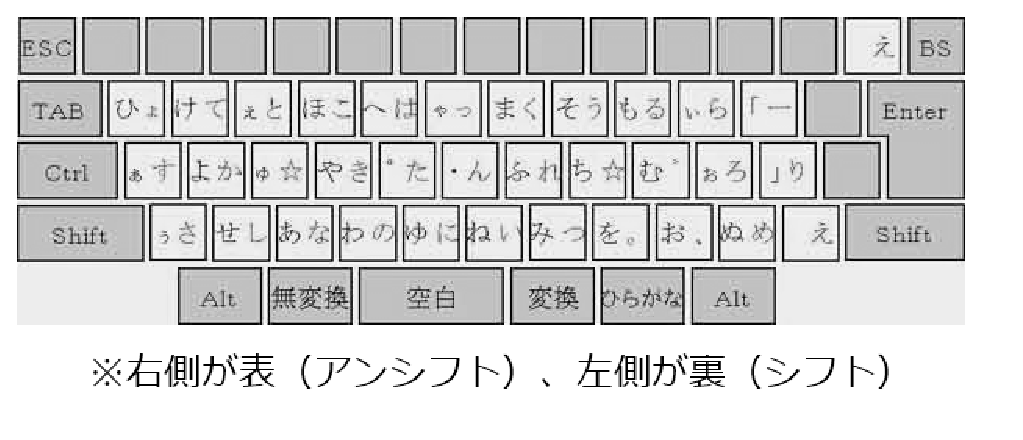
\includegraphics[width=0.8\hsize]{hana.eps}
 \end{center}
 \caption{花配列}
 \label{fig:hana}
\end{figure*}


新JISと同様、交互打鍵が約6割と多くなっています。
一方、新JISに比べ(18\%)、最下段が31\%となっており、これはJISかなの16\%と比較しても多く使われています。
これについて、冨樫氏は「手首を浮かせて打つと楽に打てる」と主張しています。

ただし、同手跳躍、同指異鍵などは、今回使用したコーパスでは新JISのほうが少なくなっていました。これは使用している文章の分野(ドメイン)の問題も大きくあると考えられます。

\subsubsection*{月配列}

2chの新JISスレッドでできたカナ系配列で、新JISに対して、前述の花配列のような中指シフトを付け加える、というアイディアのもと生まれました。
2chのスレッドにいるさまざまな人たちによって改良が重ねられ、多くの版(配列)ができました。現在では2-263(図\ref{fig:tsuki}%
\footnote{図は\url{http://jisx6004.client.jp/tsuki.html}より。}%
)と呼ばれているものが一般的です。

\begin{figure*}[htbp]
 \begin{center}
  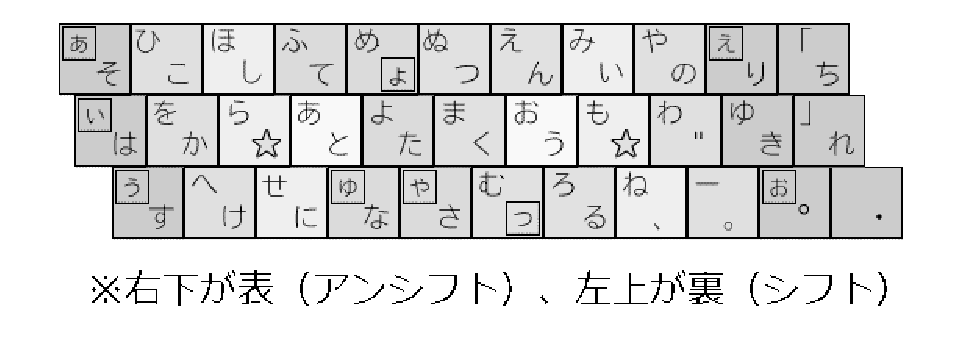
\includegraphics[width=0.8\hsize]{tsuki.eps}
 \end{center}
 \caption{月配列}
 \label{fig:tsuki}
\end{figure*}

コーパスを使ったこの配列の解析は表\ref{tbl:tsuki}のようになります。

\begin{table*}[htbp]
 \caption{月配列の解析表}
 \begin{center}
 \begin{tabular}{cccc|ccc}
 \hline
総打鍵 & 総打鍵左 & 総打鍵右 & シフト数 & 交互 & 左左 & 右右 \\
29526169 & 14294112 & 15232057 & 4819852 & 19309588 & 4639318 & 5577263\\
 & 48.4\% & 51.6\% &  & 65.4\% & 15.7\% & 18.9\%\\
 \hline
 \end{tabular}

  \vspace{1zw} 

 \begin{tabular}{ccccccccccc}
 \hline
& 左小(A) & 左薬(S) & 左中(D) & 左人(FG) & 右人(HJ) & 右中(K) & 右薬(L) & 右小(;)\\
& 5143242 & 5125313 & 2677655 & 1347902 & 4910816 & 5151515 & 4143342 & 1026384\\
左/右手中 & 36.0\% & 35.9\% & 18.7\% & 9.4\% & 32.2\% & 33.8\% & 27.2\% & 6.7\%\\
総打鍵中 & 32.2\% & 14.9\% & 19.4\% & 33.5\% & 43.9\% & 32.2\% & 21.5\% & 2.3\%\\
\hline
 \end{tabular}

  \vspace{1zw} 

 \begin{tabular}{ccc|cccc}
 \hline
 同指異鍵 & 同手跳躍 & 左手縦 & 最下段(ZX..) & ホーム(AS..) & 三段目(QW..) & 最上段(12..)\\
2322072 & 996617 & 50003 & 5138841 & 15676342 & 8632038 & 78948\\
 &  &  & 17.4\% & 53.1\% & 29.2\% & 0.3\%\\
\hline
 \end{tabular}
 \end{center}
 \label{tbl:tsuki}
\end{table*}

%\begin{table}[htbp]
% \begin{center}
%  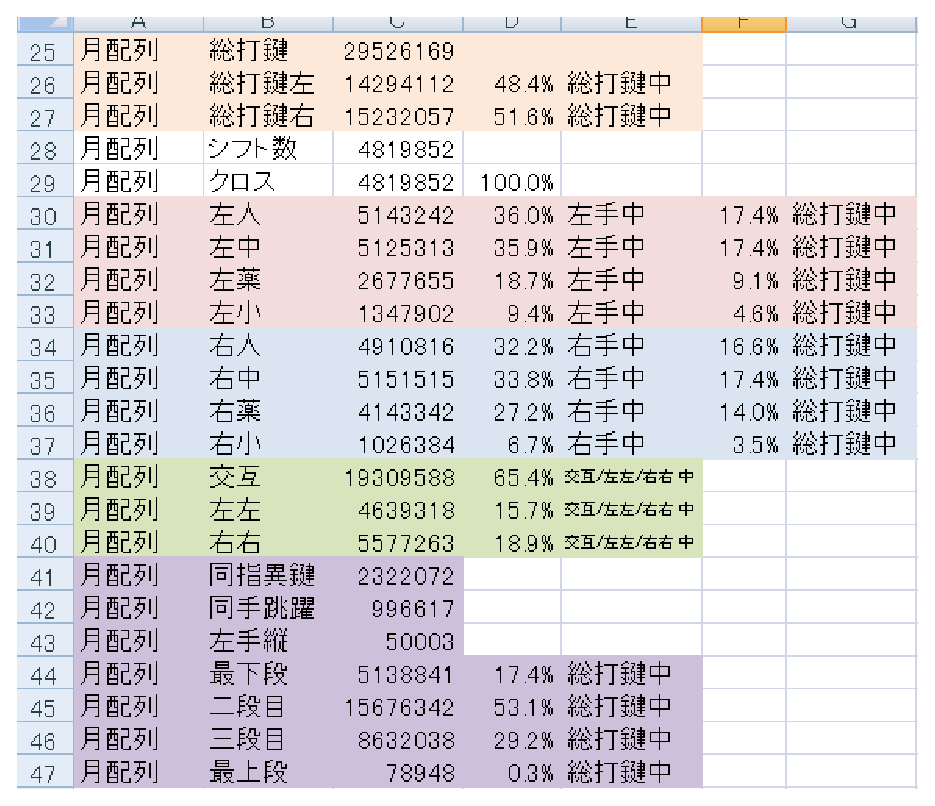
\includegraphics[width=0.85\hsize]{tbl-tsuki.eps}
% \end{center}
% \caption{月配列の解析表}
% \label{tbl:tsuki}
%\end{table}

新JISの持っていた6割という交互打鍵率をこの配列も保っています。新JISに比べ、左左/右右がバランスよく含まれており、両手をより均等に使った配列と言えるでしょう。

\subsection{親指シフト系}
\subsubsection*{NICOLA}

OASYS配列、またはNICOLA配列は「親指シフト配列」と呼ばれ、
キーボードのスペースキーにあたるところに、図\ref{fig:nicola}のような二つの「親指シフトキー」をおいてあるのが特徴です。

図\ref{fig:nicola}のキーには三つ仮名が書いてありますね。
下にある文字はそのまま打ち、上にある文字は「その文字と同じ手でシフトを押しながら」(同手シフト)打ちます。
濁音については、「清音のキーと反対側の手でシフトを押しながら」(クロスシフト)打ちます。
この仕様のため、親指シフトでは、清音(濁音が付く文字)はすべて単独で打てる文字となっています。

\begin{figure*}[htbp]
 \begin{center}
  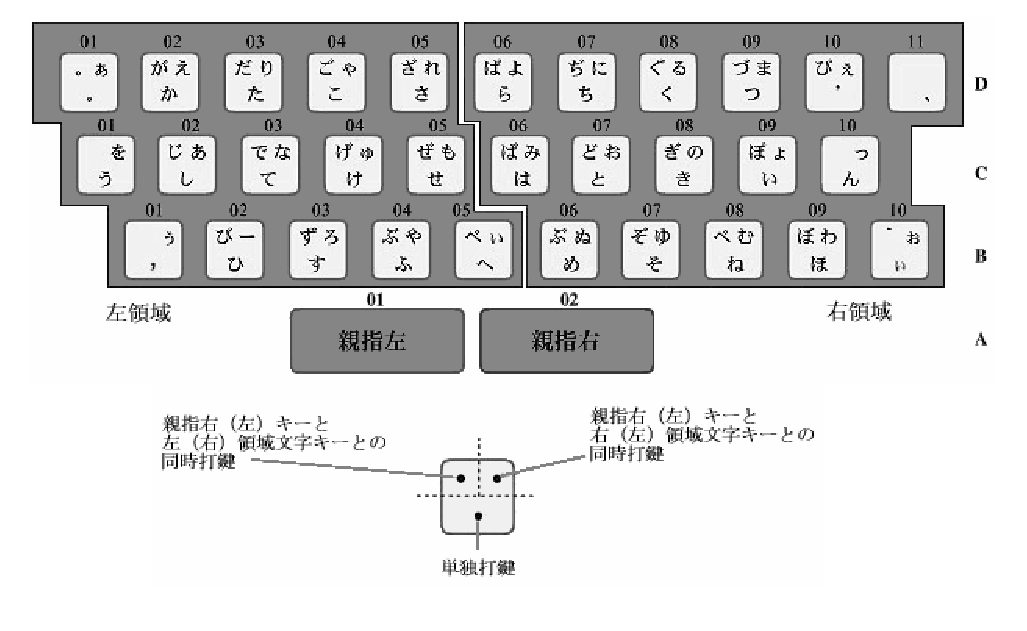
\includegraphics[width=0.8\hsize]{nicola.eps}
 \end{center}
 \caption{NICOLA配列(図はNICOLA配列規格書より)}
 \label{fig:nicola}
\end{figure*}

親指シフト配列の起源は、1980年、富士通のOASYS100というワープロ専用機に始まります。
初代以降、一貫してOASYSは親指シフトを採用し、多くの支持者を生んできました。
日本語に適した入力方式の普及と標準化を目的として、1989年に発足した業界団体「日本語入力コンソーシアム」は、
富士通の親指シフトキーボードを改良し、「NICOLA配列」を提唱しました。

具体的な相違点としては、OASYSでは半濁音を「半濁音キー」を用いて押していたのに対し、
NICOLAでは親指で押せるようにしました。
また、最上段の記号や、バックスペース、改行キーなどの位置をNICOLAではJIS規格のキーボードに合わせています。

「キーボードを科学する」\footnote{\url{http://www.fmworld.net/oasysworld/cat/dgt01.html}}%
によると、
\begin{itemize}
\item 「人差し指がいちばん使いやすく、小指がいちばん使いにくい」
\item 「指の使いやすさは、中段(ホームポジション)、上段、下段の順」
\item 「同じ指、隣り合った指の使用は避ける」
\item 「同じ側の手ではなく、左右交互に使う方が打ちやすい」
\end{itemize}
また、(神田ら, 1979)によると
\begin{itemize}
\item 「文字の出現頻度および連接出現頻度」(unigramとbigram)を考慮
\end{itemize}
という設計思想に基づいてデザインされました。

神田らは(初代OASYSの親指シフト配列の)評価として、6人に一日0.5~1.5時間の練習を一ヶ月行わせました。その実験により、
\begin{itemize}
\item 文字キーは完全にタッチタイピングできる
\item 文字キーと親指シフトキーを同時に押すのは、キーを単独で打つのと同じ感覚で行える
\end{itemize}
ことがわかり、さらに打鍵速度として80~180字/分が得られたということです。

それではコーパスを使ってみてみましょう(表\ref{tbl:nicola})。ここでは多くの親指シフトエミュレータで採用されているNICOLA配列を評価することにします。

\begin{table*}[htbp]
 \caption{NICOLAの解析表}
 \begin{center}
 \begin{tabular}{cccc|ccc}
 \hline
総打鍵 & 総打鍵左 & 総打鍵右 & シフト数 & 交互 & 左左 & 右右 \\
 22009710 & 11180976 & 10828734 & 9331864(2892628) & 11729133 & 5316409 & 4964168\\
 & 50.8\% & 49.2\% &  & 53.3\% & 24.2\% & 22.6\%\\
 \hline
 \end{tabular}

  \vspace{1zw} 

 \begin{tabular}{ccccccccccc}
 \hline
& 左小(A) & 左薬(S) & 左中(D) & 左人(FG) & 右人(HJ) & 右中(K) & 右薬(L) & 右小(;)\\
& 2817456 & 3264915 & 3278771 & 1819834 & 3709821 & 2606899 & 2770957 & 1741057\\
左/右手中 & 25.2\% & 29.2\% & 29.3\% & 16.3\% & 34.3\% & 24.1\% & 25.6\% & 16.1\%\\
総打鍵中 & 12.8\% & 14.8\% & 14.9\% & 8.3\% & 16.9\% & 11.8\% & 12.6\% & 7.9\%\\
\hline
 \end{tabular}

  \vspace{1zw} 

 \begin{tabular}{ccc|cccc}
 \hline
 同指異鍵 & 同手跳躍 & 左手縦 & 最下段(ZX..) & ホーム(AS..) & 三段目(QW..) & 最上段(12..)\\
1834583 & 1036799 & 118061 & 2619704 & 11735857 & 7575201 & 78948\\
 &  &  & 11.9\% & 53.3\% & 34.4\% & 0.4\%\\
\hline
 \end{tabular}
 \end{center}
 \label{tbl:nicola}
\end{table*}



%\begin{table}[htbp]
% \begin{center}
%  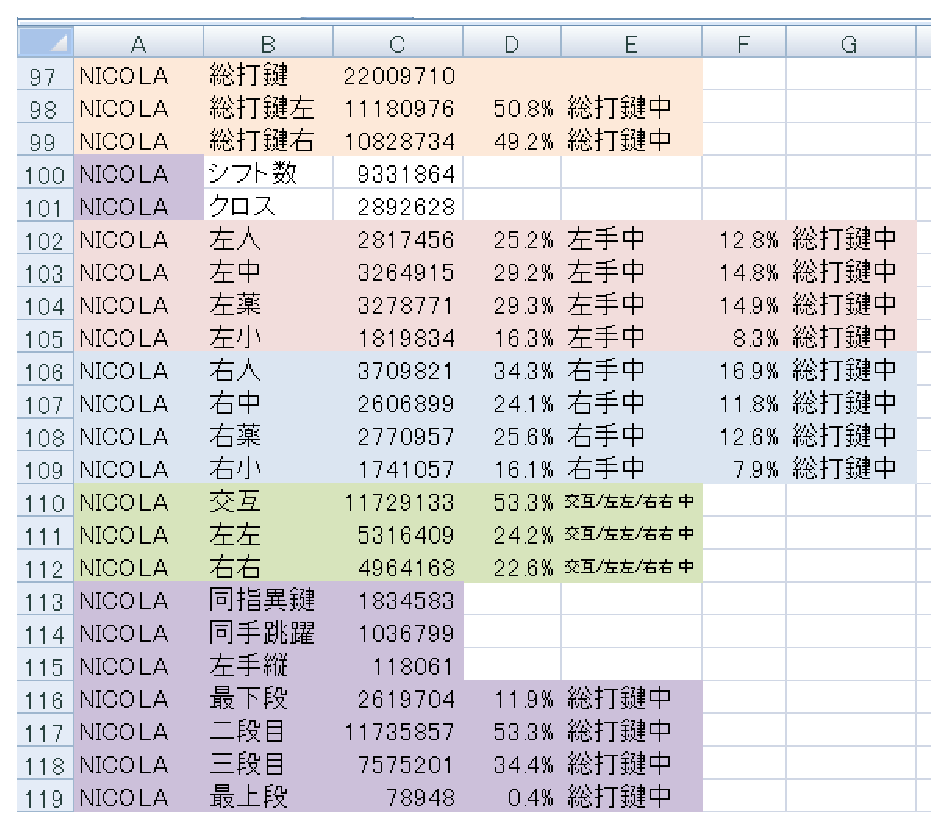
\includegraphics[width=0.85\hsize]{tbl-nicola.eps}
% \end{center}
% \caption{NICOLA配列の解析表}
% \label{tbl:nicola}
%\end{table}

NICOLAではその設計思想通り、左右バランスよく、また、ほどよく交互打鍵がされるように配列されています。
また、ホームポジションの使用率も54\%と、なるべく指から離れないようになっています。
総打鍵中43\%と4割がシフトなのは気になるところですが、ユーザテストによれば気にならないようですので、
よしとしましょう。

なお、シフト数が多いのは「の」「な」「る」などの高頻度の文字がシフトに配列されているためと考えられます。清音キーを非シフトに割り当てねばならなかった宿命でしょう。
参考のため、仮名出現上位20個のうち、裏(シフト側)になってしまった仮名を挙げます\footnote{「約」とつけると見づらいので、省略しました。すべて有効数字は2桁です。}:「の」(5位; 4.0\%)、「に」(9位; 2.8\%)、「な」(11位; 2.5\%)、「る」(15位; 2.2\%)、「っ」(18位; 2.0\%)また、逆に低頻度なのに表に来ざるを得なかった清音の仮名も挙げましょう。「へ」(0.23\%)、「ほ」(0.48\%)、「ふ」(0.48\%)、「ひ」(0.61\%)などなど。

%\subsubsection*{TRON配列}
\subsubsection*{飛鳥配列}

Ray氏によって考案された親指シフト配列である飛鳥配列は、改良に改良を重ねて作られました。その設計思想は
\begin{itemize}
\item 右手をよく使う\footnote{左利きの人用に「レフティ飛鳥」というものも用意されています。}
\item 親指キーを押しっぱなしにした状態での連続入力(裏のキーを連続で入力する)ことを積極的に取り入れている(cf. NICOLAでは一打鍵ごとに一シフト)
\end{itemize}

飛鳥配列はその歴史から大量に版があります%
\footnote{今回用いたのは、飛鳥配列383版のうち、数字の配列が123\ldots となっている「飛鳥配列123-383版」です。}
が、その一例を図\ref{fig:asuka}に示します%
\footnote{図は\url{http://ameblo.jp/asuka-layout/entry-10334710008.html}より。}%
。「がぎぐげご」などの濁音も一つのキーで入力するのが特徴です。

\begin{figure*}[htbp]
 \begin{center}
  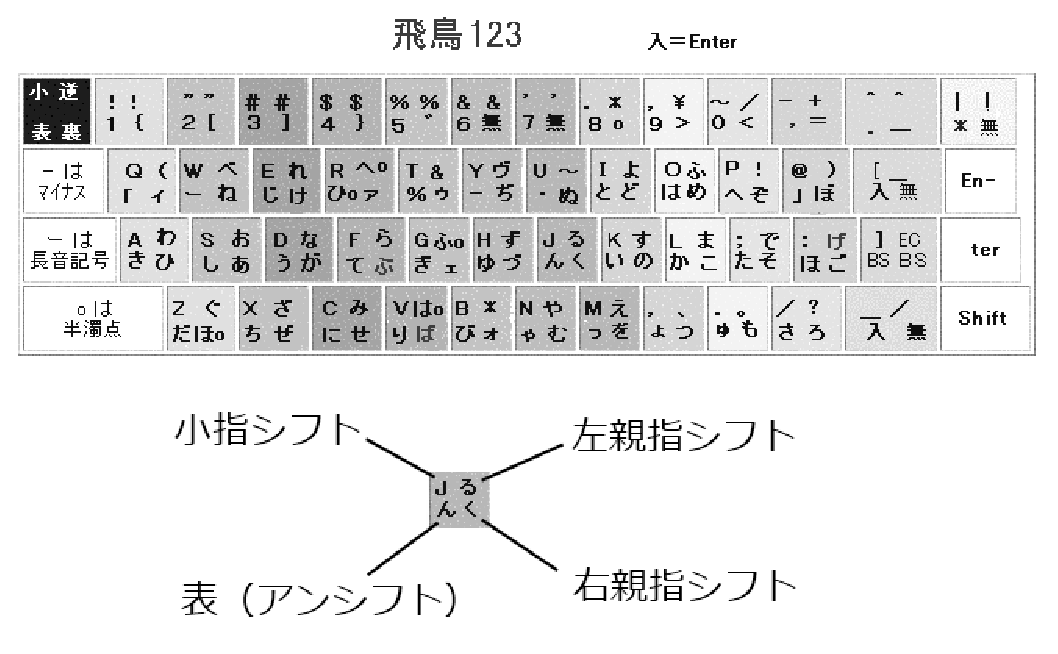
\includegraphics[width=0.8\hsize]{asuka.eps}
 \end{center}
 \caption{飛鳥配列123-383版}
 
 \label{fig:asuka}
\end{figure*}

それではコーパスを使って評価してみます。
%(今回の評価プログラムでは、「シフトを押しっぱなしの連続入力」を定量的に量ることに対応していませんでした。次回以降の課題とします)。

\begin{table*}[htbp]
 \caption{飛鳥配列の解析表}
 \begin{center}
 \begin{tabular}{cccc|ccc}
 \hline
総打鍵 & 総打鍵左 & 総打鍵右 & シフト数 & 交互 & 左左 & 右右 \\
22329794 & 8913749 & 13416045 & 10594571(5240353) & 11489323 & 3169088 & 7671383\\
 & 39.9\% & 60.1\% &  & 65.5\% & 18.1\% & 43.8\%\\
 \hline
 \end{tabular}

  \vspace{1zw} 

 \begin{tabular}{ccccccccccc}
 \hline
& 左小(A) & 左薬(S) & 左中(D) & 左人(FG) & 右人(HJ) & 右中(K) & 右薬(L) & 右小(;)\\
1575536 & 3914260 & 2128521 & 1295432 & 3437742 & 4878650 & 3246516 & 1853137\\
左/右手中 &17.7\% & 43.9\% & 23.9\% & 14.5\% & 25.6\% & 36.4\% & 24.2\% & 13.8\%\\
総打鍵中 & 7.1\% & 17.5\% & 9.5\% & 5.8\% & 15.4\% & 21.8\% & 14.5\% & 8.3\%\\
\hline
 \end{tabular}

  \vspace{1zw} 

 \begin{tabular}{ccc|cccc}
 \hline
 同指異鍵 & 同手跳躍 & 左手縦 & 最下段(ZX..) & ホーム(AS..) & 三段目(QW..) & 最上段(12..)\\
1988288 & 930019 & 20753 & 6033749 & 12828047 & 3389059 & 78939\\
 &  &  & 27.0\% & 57.4\% & 15.2\% & 0.4\%\\
\hline
 \end{tabular}
 \end{center}
 \label{tbl:asuka}
\end{table*}

%\begin{table}[htbp]
% \begin{center}
%  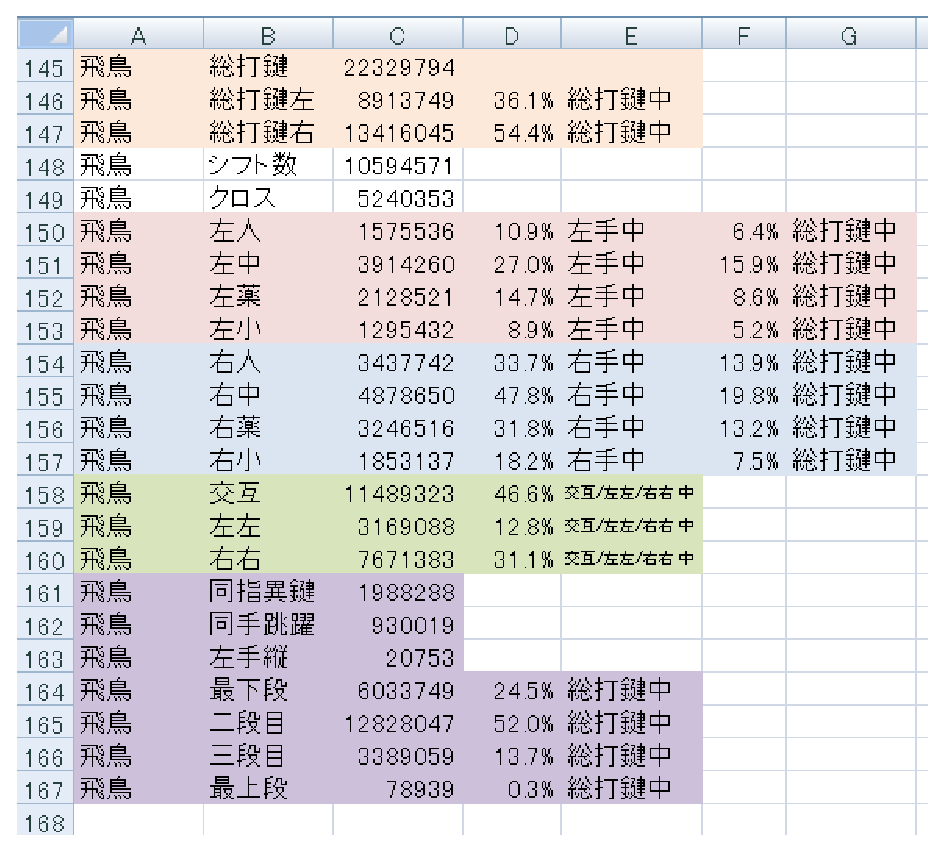
\includegraphics[width=0.85\hsize]{tbl-asuka.eps}
% \end{center}
% \caption{飛鳥配列(383版)の解析表}
% \label{tbl:asuka}
%\end{table}

設計思想通り、右手の使用率が約54\%と高くなっています。また、交互打鍵率が約47\%、続いて右→右の入力が約31\%と、交互打鍵もしつつ、得意な右手を使ってあげるという、バランスのとれた配列になっています。

特筆すべきは左手縦連の少なさです。NICOLAのそれと比べての17\%という少なさです(飛鳥: 20753、NICOLA: 118061)。
飛鳥配列はシフトを押したままの連続入力にあくまでもこだわった結果、アルペジオ運指を多く生み出したのでしょうか(今回使用した解析スクリプトでは、アルペジオ運指は考慮していませんでした。次回以降の課題とします)。

また、最下段の使用もNICOLAに比べて多く、花配列と同様、(パームレストなどを使って)手を浮かせて入力するのに向いていると考えられます。

\subsection*{小梅配列}

小梅配列はNICOLA、TRON配列、飛鳥配列の流れをくむ親指シフト配列で、クロスシフトで濁音を入力する特徴を持っています(図\ref{fig:koume}%
\footnote{図は\url{http://homepage2.nifty.com/61degc/reports/koume/} より。})。

設計思想として、NICOLAと同様にクロスシフトで濁音を入力し、記憶に対する負荷を減らしています。連続シフトではなく、その都度シフトを入力させる点もNICOLAと同様です。
また、交互打鍵率を高くする一方で、多くの人の利き手である右手の使用頻度を高くしています。具体的には、左右の使用頻度を左手:右手=43:57と設定しています(後述するように、これはコーパスでも確認できます)。

\begin{figure*}[htbp]
 \begin{center}
  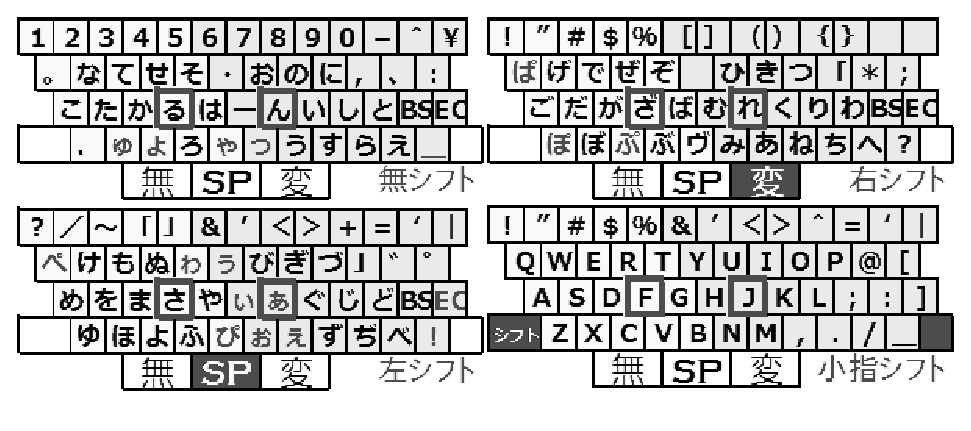
\includegraphics[width=0.8\hsize]{koume.eps}
 \end{center}
 \caption{小梅配列}
 \label{fig:koume}
\end{figure*}

それではコーパスを使って評価してみます。%(今回の評価プログラムでは、「シフトを押しっぱなしの連続入力」を定量的に量ることに対応していませんでした。次回以降の課題とします。)
左手:右手の使用頻度が約44:56と、設計思想通りになっていることがうかがえます。また、交互打鍵率・右手使用率(右→右)もともに高くなっています。

\begin{table*}[htbp]
 \caption{小梅配列の解析表}
 \begin{center}
 \begin{tabular}{cccc|ccc}
 \hline
総打鍵 & 総打鍵左 & 総打鍵右 & シフト数 & 交互 & 左左 & 右右 \\
 22366745 & 9793272 & 12573473 & 8115349(2609182) & 12832519 & 3377012 & 6157214\\
 & 43.8\% & 56.2\% &  & 57.4\% & 15.1\% & 27.5\%\\
 \hline
 \end{tabular}

  \vspace{1zw} 

 \begin{tabular}{ccccccccccc}
 \hline
& 左小(A) & 左薬(S) & 左中(D) & 左人(FG) & 右人(HJ) & 右中(K) & 右薬(L) & 右小(;)\\
& 2620589 & 3462294 & 2461322 & 1249067 & 4025676 & 3719075 & 3191966 & 1636756\\
左/右手中 & 26.8\% & 35.4\% & 25.1\% & 12.8\% & 32.0\% & 29.6\% & 25.4\% & 13.0\%\\
総打鍵中 & 11.7\% & 15.5\% & 11.0\% & 5.6\% & 18.0\% & 16.6\% & 14.3\% & 7.3\%\\
\hline
 \end{tabular}

  \vspace{1zw} 

 \begin{tabular}{ccc|cccc}
 \hline
 同指異鍵 & 同手跳躍 & 左手縦 & 最下段(ZX..) & ホーム(AS..) & 三段目(QW..) & 最上段(12..)\\
1962705 & 1135597 & 18698 & 4734636 & 10838801 & 6627420 & 165888\\
 &  &  & 21.2\% & 48.5\% & 29.6\% & 0.7\%\\
 &  &  & 総打鍵中 & 総打鍵中 & 総打鍵中 & 総打鍵中\\
\hline
 \end{tabular}
 \end{center}
 \label{tbl:roma}
\end{table*}

%\begin{table}[htbp]
% \begin{center}
%  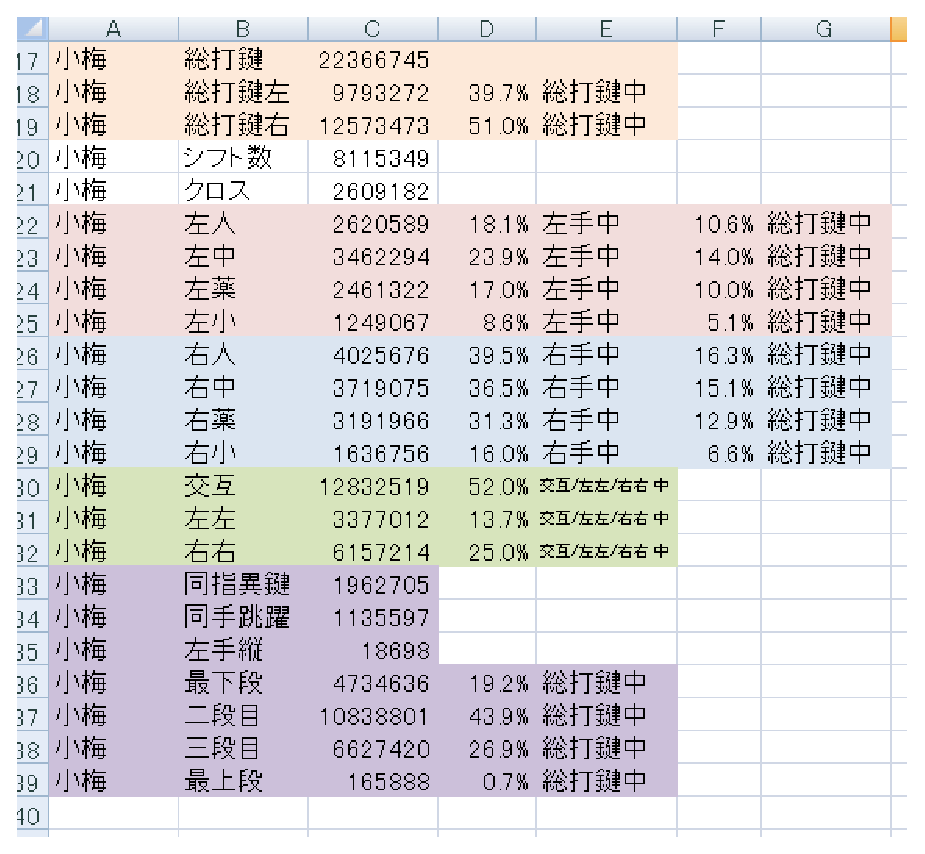
\includegraphics[width=0.85\hsize]{tbl-koume.eps}
% \end{center}
% \caption{小梅配列の解析表}
% \label{tbl:koume}
%\end{table}

\subsection{遺伝的アルゴリズムによる配列決定}

前述の花配列のおさらいをしましょう。花配列では、「よい配列」をまず定義し、ランダムな配置から初めて、組み合わせを少しずつ「よい方向へ」変えていったのでした。
このように、「よさ」({\bf 評価値})を定義して、評価値のできるだけ高い(最大となるのが望ましい)解を求める問題を「探索問題」と言います。
特に、解が配列のような組み合わせの場合、「{\bf 組み合わせ最適化問題}」と呼びます。

一般に、組み合わせ最適化問題は組み合わせの数が膨大になってしまうため、探索が困難です。たとえば、仮名の文字55個と記号8個の計63個を単純に並べる並べ方は$63!$通りです。
これは$10^{87}$よりも$2^{289}$よりも大きい数で、この組み合わせをすべて探索(全解探索、あるいは全探索といいます)するのは現実的ではありません。

そこで、全探索をしないでできるだけよい解を求めるアルゴリズムがいくつも存在します。今から説明するのは、生物の遺伝子を模した「遺伝的アルゴリズム」というものです。
{\bf 遺伝的アルゴリズム}は、解の候補を「遺伝子」という形で表現し、それらを「かけあわせ」(\ruby{{\bf 交叉}}{こうさ})て新しい個体(解)を生成し、
さらに評価値によって「一部のみ生き残らせる」(=自然\ruby{淘汰}{とうた}; {\bf 選択})ことを繰り返すことによって、よりよい解を探索します。
また、交叉の際に解の一部を変化させる(突然{\bf 変異})こともします。
このように、生物の進化を模しているため、進化的アルゴリズムの一種とされます。

しかし、ある仮名配列と仮名配列を単純にかけあわせる(混ぜる)だけでは、同じキーが二カ所出てきたり、存在しないキーが出てきたりと、使いものにならない配列ができてしまいます。
このような配列(遺伝子)を「{\bf 致死遺伝子}」と言います。
致死遺伝子を発生させない交叉をどう実現するか、あるいはそもそも遺伝子をどう表現するかは、とても難しい問題です。

また、評価値の計算も重要です。遺伝的アルゴリズムでは、単一の評価値を用いて生き残る遺伝子を決めていました。
適切な評価基準を用いないと、ふさわしくない遺伝子が生き残ってしまうことになり、やはりよい解は得られません。

このように使いどころが難しい遺伝的アルゴリズムですが、
一般に全探索が困難な問題に対してそれなりに良い解が求められるということで、
一時期、一世を\ruby{風靡}{ふうび}したという過去を持ちます。

\subsubsection*{先行研究(仮名配列以外)}

遺伝的アルゴリズムによるキーボード配列設計では、北インドで話されているヒンディー語の
キーボードの設計 [Deshwal and Kalyanmoy, 2003]や、アルファベットのソフトウェアキーボードの設計 [Raynal and Vigouroux, 2005] などで行われています。

Deshwalらの設計では、二つの遺伝子(配列)$G_1$と$G_2$があったとき、まず$G_1$の半分を残し、
残りの半分のキーを$G_2$のキーの「近く」に並べ替える(=$G_2$のキーを参考にして改良する)
ことで、致死遺伝子を作ることなく交叉を実現しています。
また、評価関数として、交互打鍵率を増やす、同じ指でキーを打たない、などを用いています。

Raynalらは、前提知識編で紹介したフィッツの法則を用いています。ソフトウェアキーボードではマウスやペンを使うので、フィッツの法則がクリティカルに効いてくるのでしょう。

\subsubsection*{幸花配列(旧名:○配列)}

遺伝的アルゴリズムを中指シフト仮名配列の設計に用いたのが、幸花配列(旧名:○配列)です%
\footnote{\url{http://www.geocities.jp/rage2050a/GeneKana/_ReadMe.html}}%
(図\ref{fig:maru})。

\begin{figure*}[htbp]
 \begin{center}
  \includegraphics[width=0.8\hsize]{maru.eps}
 \end{center}
 \caption{○配列}
 \label{fig:maru}
\end{figure*}

交叉は、ランダムにキーの位置を選び、ランダムに配列(遺伝子)$G_1$、$G_2$のどちらかを選んでいき、
すべてのキーに仮名を置くまで繰り返す、というものです。
競合が起こる(同じ仮名がすでに置かれている)場合には、
キー配列の左上から順にまだ置かれていないものを選ぶ、という方法で解決しています。
評価には開発者が自身でキーのbigramについて打鍵時間を計測し、その組み合わせを用いました。

それではコーパスを使って評価してみましょう(表\ref{tbl:maru})。

\begin{table*}[htbp]
 \caption{○配列の解析表}
 \begin{center}
 \begin{tabular}{cccc|ccc}
 \hline
総打鍵 & 総打鍵左 & 総打鍵右 & シフト数 & 交互 & 左左 & 右右 \\
29756111 & 14149812 & 15606299 & 5049787 & 19866174 & 4216725 & 5673212\\
 & 47.6\% & 52.4\% &  & 66.8\% & 14.2\% & 19.1\%\\
 \hline
 \end{tabular}

  \vspace{1zw} 

 \begin{tabular}{ccccccccccc}
 \hline
& 左小(A) & 左薬(S) & 左中(D) & 左人(FG) & 右人(HJ) & 右中(K) & 右薬(L) & 右小(;)\\
& 5020769 & 4841928 & 2420872 & 1866243 & 4788744 & 4902439 & 4506402 & 1408714\\
左/右手中 &35.5\% & 34.2\% & 17.1\% & 13.2\% & 30.7\% & 31.4\% & 28.9\% & 9.0\%\\
総打鍵中 & 16.9\% & 16.3\% & 8.1\% & 6.3\% & 16.1\% & 16.5\% & 15.1\% & 4.7\%\\
\hline
 \end{tabular}

  \vspace{1zw} 

 \begin{tabular}{ccc|cccc}
 \hline
 同指異鍵 & 同手跳躍 & 左手縦 & 最下段(ZX..) & ホーム(AS..) & 三段目(QW..) & 最上段(12..)\\
2003058 & 1082831 & 47820 & 5960127 & 16389169 & 7327867 & 78948\\
 &  &  & 20.0\% & 55.1\% & 24.6\% & 0.3\%\\
\hline
 \end{tabular}
 \end{center}
 \label{tbl:maru}
\end{table*}

%\begin{table}[htbp]
% \begin{center}
%  \includegraphics[width=0.85\hsize]{tbl-maru.eps}
% \end{center}
% \caption{○配列の解析表}
% \label{tbl:maru}
%\end{table}

交互打鍵率が約67\%と、花、月配列を若干上回る高さです。
評価値には実測の打鍵時間が用いられているので、交互打鍵の速さを実感できます。

ホームポジションの打鍵率も約55\%と、月、花よりも多くなっています。
左手縦連の少なさ(幸花:47820、花:83290、月:50003)も魅力的です。

\subsection{まとめ}

最後に、今まで出てきた配列をまとめて比較してみましょう(表\ref{tbl:matome}と表\ref{tbl:matome-percent})。
なお、表\ref{tbl:matome-percent}のパーセント表記は、
\begin{itemize}
 \item 総打鍵左・右は総打鍵中の割合
 \item シフト・クロスシフトは総打鍵中の割合
 \item 左\{小薬中人\}・右\{人中薬小\}は総打鍵中に占める割合
 \item (1)交互・(2)左左・(3)右右は、この三つの割合。つまり $ \frac{(1)}{\left\{(1)+(2)+(3)\right\}} $ などの割合。
 \item 最下段~最上段はそれぞれの全打鍵に占める割合(=総打鍵における割合)
\end{itemize}
です。

AZIKのタイプ数の削減率は、中指シフト配列に迫る勢いです。気になるのは左手小指の使用率の高さですが、これはおもに\key{Q}と(前に右手のキーが続くときの-anである)\key{Z}によるものです。実際の運指では、特に「かん」(\key{K}\key{N})などは右だけで打つこともあるため、やや強引な仮定だったかもしれません。

交互打鍵については今回、「中指シフトはすべてクロスシフト」という仮定をおいたため、花/月/幸花(○)配列に有利になっています。
実際の運指によってはアルペジオ運指になることも十分ありえますので、結果を見るときはご注意願います。

交互打鍵を主眼においた新JIS、NICOLA、小梅に比べて、飛鳥配列の交互打鍵率がやや低くなっているのが見てとれます。
飛鳥配列ではその代わり、右右の比率が多くなっており、アルペジオ運指を狙っていることが示唆されます。%
%(ただし、今回の解析プログラムでは、アルペジオについては調べることができませんでした)。

人差し指は二列を担当するため、一般的に使用比率が高くなりがちです。実際、多くの配列で「左人/右人」の値は高くなっています。
一方、飛鳥配列については人差し指の使用率が低くなっていることに注目しましょう。これは飛鳥配列の設計思想の一つ、「人差し指のうち、\key{T}と\key{Y}のある列は遠いので避ける」を反映しているものと言えましょう。

\subsection{あとがき}

今回はQWERTY、および仮名配列に焦点を当てていました。
そのため、Dvorakや、AZIKのDvorak版であるACTに触れることができませんでした。
また、飛鳥配列における連続シフト(アルペジオ運指)についての研究もできませんでした。

先行研究において、「(親指の)シフト動作はタイピングに影響を及ぼさない」とあったとはいえ、
筆者の実感ではシフト動作はわりと指(と頭)に負担がかかっているような印象を受けます。

次回、またこのような文章を書く機会があれば、もっと細かい部分まで凝らした考察を載せたいと考えています。
また、当初の目的であった「打ちやすい」キーボード配列を求めて、配列設計についても文章を\ruby{認}{したた}めたい
です。特に筆者はAZIKに大きな可能性を見いだしているため、今回書いたような知見を活かし、AZIKの最適配置を
計算によって求めたいと思っています。では、またどこかで。

\clearpage

\begin{table*}[htbp]
 \caption{まとめ(値は1000で割ってある)}
 \begin{center}
  \includegraphics[angle=90, width=0.85\hsize]{matome-table.eps}
 \end{center}
 \label{tbl:matome}
\end{table*}

\clearpage

\begin{table*}[htbp]
 \caption{まとめ(パーセント表記)}
 \begin{center}
  \includegraphics[angle=90, width=0.85\hsize]{matome-table-percent.eps}
 \end{center}
 \label{tbl:matome-percent}
\end{table*}



\clearpage
\articlepart{タイピングとキーボード}{eigh}

\section{はじめに}
タイパーにとってキーボードと言ったらどんな存在でしょうか。キーボードはタイピングにおいて必要不可欠な道具であり、タイピングに大きな影響を与えています。しかし、キーボードとタイパーの関係というのは人によって様々だと思います。「キーボードを変えて新記録を出しても実力が伸びたわけじゃないからキーボードを替えたくない」という人や「記録が伸びるならキーボードを替える」という人、「いろんなキーボードの打鍵感を楽しみたい」などいろいろな人がいると思います。 今回はキーボードがタイピングの速さにどのように関わっているかを簡単な実験や主観を交えながら考えていきたいと思います。

\section{タイピングにおけるキーボード}

\subsection{なぜキーボードにこだわるか}
どのタイパーも、程度の違いはあれキーボードを替えることによりタイピングの速さは変わります。また、タイピングの速さだけでなく成長速度にも影響しているようで、キーボードを替えたことによって記録が伸びたタイパーも少なくありません。ではキーボードのどのような要素がタイピングの速さに影響を与えているのでしょうか。

\subsection{タダの入力機器なのか?}
キーボードを物理的な側面から捉えると、各キーごとのスイッチによってPCへ電気信号を入力する機器と見ることができます。この関係をシンプルに表現すると図\ref{eigh:img1}のようになります。しかし、このような一方通行の関係では、タイピングに与えている影響を読み取ることができません。現実にタイピングの速さ(言い換えるとタイパーの打鍵動作)に大きく影響していることを考えると、キーボード自体がタイパーにもなんらかのフィードバックを行っている「タイパーへの入力装置」としての働きがあると考えることができます。これを示したのが図\ref{eigh:img2}になります。

\begin{figure*}
 \begin{center}
   \includegraphics[width=14cm,clip]{res_eigh/img1.eps}
 \end{center}
 \caption{タイパーとキーボード、PCとの関係}
 \label{eigh:img1}
\end{figure*}

\begin{figure*}
 \begin{center}
   \includegraphics[width=14cm,clip]{res_eigh/img2.eps}
 \end{center}
 \caption{キーボードからタイパーへの「入力」}
 \label{eigh:img2}
\end{figure*}

タイピング中は、キーボードはタイパーからPCへキー情報を入力するだけでなくタイパーへも多くの情報を入力し、タイピングに影響していると考えられます。

\subsection{キーボードからの情報}

ではタイピング中にどのような情報が入力されるのでしょうか。五感の中でキーボードに関係するのは主に聴覚と触覚です。音の情報も重要だとは思いますが、やはりキーボードから得られる情報で重要な要素は触覚情報、つまりキーの反発の仕方であると考えます。では具体的にキーボードの荷重特性\footnote{簡単にいえばキーを押すにはどれくらいの力が必要か、という特徴。キーボードやその構造によって大きく異なる。}を見ることで、反発のどのような要素がタイパーへの入力と解釈できるか詳しく見てみます。

\subsection{一般的なキーボードの荷重特性}

キーボードの特徴を表現するために荷重特性というグラフがよく用いられます。一般的なキーボードの荷重特性から見てみましょう。図\ref{eigh:img4}は一般的なラバードーム\footnote{半球状のゴム製の部品}を使用したキーボードにおける荷重特性のグラフです。実際にこのような荷重特性を持つキーボードがあるというわけではありませんが、多くのキーボードでこのようなグラフを描きます。横軸はキーを押した深さ、縦軸はキーボードからの反発力を表しています。

\begin{figure*}
 \begin{center}
   \includegraphics[width=14cm,clip]{res_eigh/img4.eps}
 \end{center}
 \caption{キーボードの荷重特性}
 \label{eigh:img4}
\end{figure*}

このグラフの特徴を右に進みながら見てみましょう。まず、ある点まで反発力が増加していき、そこを頂点に減少しはじめます。ある点まで減少が続き、再び増加へと転じます。最後は値がどんどん大きくなっていきます。とりあえずここでは最初の頂点を「山」、次に一番低くなる場所を「谷」、最後に急激に重さが増える点を「壁」と呼ぶことにします。一般的にキーボードのスペックとして荷重の重さとストロークの深さが書かれていることがありますが、その二つはここでいう山の高さと壁までの距離、ということになります。これらを示したものが図\ref{eigh:img5}になります。

\begin{figure*}
 \begin{center}
   \includegraphics[width=14cm,clip]{res_eigh/img5.eps}
 \end{center}
 \caption{荷重特性とキーボードの入力}
 \label{eigh:img5}
\end{figure*}

\subsection{どの部分を入力とするか}
キーボードの打鍵感について、「クリック感」と「底打ち感」という言葉がよく使われます。クリック感というのは山から谷へかけての部分で、この差が大きい物がクリック感が強いとかはっきりしていると言われます。また、底打ち感を感じるのは壁の部分で、グラフの傾きが大きい(急激に変化している)ものほど底打ち感がはっきりしていると言われます。この「クリック感」「底打ち感」両方に言えることは、傾きが大きいほどはっきり感じるということです。この傾きが一種の入力となっているといっていいでしょう。今回はこれら2つを「クリック」「底打ち」と呼び、キーボードからの「入力」として扱うことにします。

\section{「速い」キーボードの特徴}
「クリック」や「底打ち」という入力に要する時間や感触の強さはキーボードによって、大きく異なります。実際に速く打てると言われているキーボードの特徴を考え、入力がどのようにタイピングの速さに影響しているか見てみましょう。
速く打てるキーボードと言っても人によって相性があったり慣れの問題もあるため一概には言えませんが、タイパーによく使われているキーボードとしては東プレのリアルフォース(リアフォ)とパンタグラフ式のキーボード(パンタ)が挙げられます。この2つのキーボードはどちらも反発が軽い、ストロークが浅いという特徴を持っています。これらの特徴についてキーボードからの入力の時間、強さという観点から考えてみます。

\subsection{入力に要する時間}

\begin{figure*}
 \begin{center}
   \includegraphics[width=14cm,clip]{res_eigh/img3.eps}
 \end{center}
 \caption{タイパーとキーボードの時間軸上の流れ}
 \label{eigh:img3}
\end{figure*}

図\ref{eigh:img3}のような時間軸上でキーボードとタイパーの相互の影響を見てみると、タイパーが動作を行うことでキーボードの反発の仕方が変わり、それが再びタイパーへの入力になるという流れになります。タイピング中は、タイパーの動作とキーボードからの入力が繰り返されることから、このループの周期が短くなるほどタイピングが速くなります。つまり、タイパーの反応速度(入力から動作までの時間)だけでなく、キーボードの反応時間(タイパーの動作からタイパーへ入力するまでの時間)もタイピングの速さに関係しているということです。この反応時間がキーボードによって異なることから、結果的にキーボードによってタイピングの速さに差が生まれます。ここでは、「タイパーの動作開始」から「クリック入力」までの1サイクルを「反応時間」としています。


\subsubsection*{実験}
キーボードの反応時間は「キーボードの荷重特性」と「キーを押す強さ(速さ)」によって変わります。ここでは、異なる荷重特性を持つ仮想キーボードを用意し、一定の強さでキーを押し込んでいった際の反応時間を計算で求めることで、キーボードの特徴をよりわかりやすく示します。この実験では、基準となるキーボード(基準)、浅いキーボード(浅い)、軽いキーボード(軽い)の3種類の荷重特性(ある位置$x$における反発力の関数)を用意しました。

まず計算方法の説明ですが、キーを押す強さと反発力からキーが押し込まれていく速度が決まり、そこからある時刻のキーの位置やクリックが発生するまでの時間を求めることができます。これらをまとめたものが次の運動方程式になります。高校物理で習った方も(そしてすでに忘れている方も)いらっしゃると思いますが、$F=ma$という運動の公式を使っています。

\[
v(t+1)= v(t) + \frac{F(x)-R(x)}{m}
\]

\noindent $v(t)$:時刻tにおけるキーの速度$[m/s]$ \\
\noindent $F(x)$:位置($x$)におけるキーを押す力(谷までは一定の力、谷に到達したあとは0)$[N]$ \\
\noindent $R(x)$:位置($x$)におけるキーの反発力$[N$] \\
\noindent $m$:指の質量(定数)$[kg]$ \\

\[
x(t+1) = x(t+1) + v(t)
\]
\noindent $x(t)$:時刻$t$におけるキーを押し込んだ位置 $[m]$
 \\

初期値としてキーを押す力$F$、反発力$R$、質量$m$を決めたのちに時刻$t$を徐々に動かしていき、位置$x$が「クリック」「底打ち」「戻り」に到達する時刻を求めます。計算式でイメージしづらい方は以下の流れをご覧下さい。この実験では位置X1、X3、X0に到達するまでの時間を求めます。

\begin{enumerate}
 \item 位置X0:一定の強さで押しはじめる(位置によって反発力が変化していく)
 \item 位置X1:「クリック」に到達する
 \item 位置X2:「谷」に到達する(押す力を0にする)
 \item 位置X3:「底打ち」に到達する
 \item 反発力でキーが戻っていく
 \item 位置X0:「戻り」に到達する
\end{enumerate}

今回は反発力Rの山を「基準」と「浅い」で55g、「軽い」で44gとしました。実験で使った値は荷重特性のグラフのように複雑に変化させていますが、ここでは特徴的な値のみとさせていただきます。また、それぞれの到達位置は「基準」と「軽い」で山、クリック、谷、底打ちの順に、1mm、1.75mm、2.5mm、3.9mmとし、「浅い」は前者を1.4で割った値としました。キーを押す力は102gです。

上記のようなパラメータで実験したところ、表\ref{eigh:result}のような結果が得られました。基準キーボードに対して浅いキーボードは全ての位置に短い時間で到達しています。一方、軽いキーボードではクリックと底打ちまでの時間は短くなっていますが、反発力が弱いために戻るのに余計に時間を要しています。この結果は、軽いキーボードでは同一キーの連打や同じ指を連続で使用する場合に遅くなってしまう可能性があることを示しています。

\begin{table}
\begin{center}
\caption{実験結果}
\label{eigh:result}
\begin{tabular}{|c|c|c|c|}
\hline
 & \multicolumn{3}{|c|}{時間 [ms]} \\
\hline
キーボード & クリック & 底打ち & 戻り \\
\hline
基準 & 25 & 43 & 82 \\
\hline
軽い & 24 & 40 & 83 \\
\hline
浅い & 21 & 36 & 68 \\
\hline
\end{tabular}
\end{center}
\end{table}

\subsection{入力の強さ}
キーボードからの入力に反応してタイピングの動作を行なっていく場合だけでなく、図\ref{eigh:img6}のようにキーボードからの入力を無視して打つような場合もあると思います。このような打ち方をする場合はキーボードからの入力(クリック感や底打ち感)は弱いほうが反応を無視しやすく、打つのが容易になります。

これまで筆者が打ってきたキーボードの中で、入力が弱いキーボードとしてはリアフォとCHERRY社の赤軸スイッチを使用したメカニカルキーボードが挙げられます。これらのキーボードと一般的なもののキーボードの荷重特性を比べた結果が図\ref{eigh:img7}になります。山から谷にかけての変化が小さかったり谷がまったくなかったりしています。筆者の経験では、このような入力が弱いキーボードでは「邪魔されないで打てる」という感覚があります。

\begin{figure*}
 \begin{center}
   \includegraphics[width=14cm,clip]{res_eigh/img6.eps}
 \end{center}
 \caption{キーボードからの入力を無視して打つスタイル}
 \label{eigh:img6}
\end{figure*}

\begin{figure*}
 \begin{center}
   \includegraphics[width=14cm,clip]{res_eigh/img7.eps}
 \end{center}
 \caption{キーボードごとの荷重特性の違い}
 \label{eigh:img7}
\end{figure*}

\subsection{まとめ}
速いキーボードの特徴として「入力に要する時間」と「入力の強さ」から考えてみました。個人的にはこの2つの特徴で「反応がいいキーボード」と「邪魔されにくいキーボード」としています。これらは完全に両立するものではなく別の種類として考えています。人によってどちらが向いているかは違ってくると思います。自分のタイピングの特徴なども考慮しつつ、これらの特徴に注目すると良いキーボードが選べるかもしれません。

\section{打ち方とキーボード}

\subsection{パンタの特権?スライド打鍵}
パンタ特有の打ち方としてスライド打鍵と呼ばれるものがあります。これは押し込んだ指を戻さず次のキーへすべらせて打つ方法です(図\ref{eigh:img8})。打ってから戻るという動きがなくなり、その分次の動作に早く移ることができるため速く打つことができます。パンタでは短いストロークとキートップの形状によってこのスライドが非常にやりやすくなっています。実際には図のような複数の動作としてではなく、1回の動作としてやっていると思います。

\begin{figure*}
 \begin{center}
   \includegraphics[width=14cm,clip]{res_eigh/img8.eps}
 \end{center}
 \caption{スライド打鍵}
 \label{eigh:img8}
\end{figure*}

\subsection{軽いと指だけで打てる?}
キーの軽さというのは重要な要素ですが打ち方に対してどのような影響があるでしょうか。個人的には指だけで打てるというのがあります。重いキーボードではどうしても手の力も使ってしまうために同じ手が連続するような場面ではどうしても手の動きにより指の動きが制限されやすくなります。一方、指の力のみで押せるような軽いキーボードでは片手に集中するような場面でも手全体の動きに制限されにくく、このような場面でも速く打てるのではないでしょうか。

\subsection{まとめ}
キーボードによる打ち方の違いは、特定のキーボードだと特定の打ち方ができる、というよりは、ある条件下では特定の打ち方ができないと言ったものになっています。キーボードによって打ち方に制限が生まれ、速さや成長に影響しているかもしれません。

\section{改造してみよう}
キーボードは少し(?)の改造で驚くほど打鍵感が変わったりします。いくつか例を挙げたいと思います。 必ずしも速く打てるようになるとは限りませんが試してみるのもいいかもしれません。

\subsection{下に何かを敷いてみる}
キーボードの下に何か挟んでみます。挟む場所や物等によって結構打鍵感が変わります。おすすめは入手も簡単な滑り止めシートでしょうか。無駄な振動が減ってなめらかに打てるようになるような気がします。その他にも手前部分のみに本を挟みキーボードの角度を変える方法も試してみて欲しいです。慣れないと打ちにくいかもしれませんが、場合によっては打ちやすくなるかもしれません。いずれにせよ打ちにくくても戻せばいいだけなのでどんどん試してみましょう。

\subsection{荷重を軽くする}

\subsubsection*{ラバードームに切込みを入れる}
これをやってしまうと元に戻すことはできませんが、軽いキーボードが欲しい場合には試してみるのもいいかもしれません。方法は分解後にラバードームに2、3ヶ所切り込みを入れていくだけです。切り方などにもよりますが結構変わります。ただ、重さやスイッチがオンになる場所にばらつきが出てしまうためあまりお勧めしません。改造自体を目的としてやってみるのもありかもしれません。

\subsubsection*{ラバードームを潰したままの状態で放置する}

キーボードの上におもりなどを乗せ、キーが押された状態のまましばらく(数時間から1日程度)放置します。放置後にはラバードームの反発力が弱くなります。
実際に試したのは1個だけですが実際軽くなったような気がします。これをやっていない部分に比べてやった部分のキーでは明らかに軽くなっています。ばらつきが激しかったり分解が面倒だったりするラバードームを切る方法と比べるとこちらがおすすめです。

\subsection{ストロークを短くする}
キートップと本体の間に何かを挟み(図\ref{eigh:img9})ストロークを短くします。場合によってはキートップを再び付けられなくなったりするので、挟み方や材質などは制限されてしまいます。色々工夫してみるのもいいかもしれません。

\begin{figure*}
 \begin{center}
   \includegraphics[width=14cm,clip]{res_eigh/img9.eps}
 \end{center}
 \caption{キートップと本体の間に挟む}
 \label{eigh:img9}
\end{figure*}


\section{キーボードとのつきあいかた}
ここではキーボードの選び方や使い方を十数個のキーボードを打ってきた経験に基づいて色々書いていこうと思います。

\subsection{お勧めのキーボード教えて?}
打ち方など個人に依存することが大きいので単純におすすめを挙げることはできません。パンタ以外でおすすめを挙げるとするとやはりリアフォを選ぶのが無難だと思います。記録を出す手段としてのキーボード選びという事ならば、安いものをいくつも試すよりリアフォを買ってしまったほうがいいと思います。なかなか壊れませんし同時押しの問題が発生することが無いのでそれほど高い買い物にはならないでしょう。一方パンタでのおすすめというとちょっと答えにくいです。logicoolのCZ-900は人気があり非常に良いキーボードだと思うのですが、パンタとしてはやや深めのストロークで有ることから特にスライド打鍵などで打ちにくさを感じることが多いようです。とはいえ、初めてのパンタとして使うには比較的使いやすいという意見も多いのでおすすめです。


\subsection{リアフォってたくさん種類あるけどどれ選んだらいいの?}
テンキーの有無や色については好みで選べばいいでしょう。問題は荷重ですが現在売っているものは3種類あります(過去にAll55gのものも限定販売されてました)。All45gの物と30gのもの、小指以外が45gで小指の部分が30gの変荷重があります。他のキーボードを使う場合やタイピングのスタイルによって合っているものが変わってくると思います。

\subsubsection*{変荷重}
そこそこお勧めです。力の弱い小指部分が軽くなっており、そこがいい部分であり、悪い部分であると言えます。小指の部分が他の指の部分と感覚が異なるためキーボードからの入力が指によって異なり、リズムが取りにくくなるかもしれません。また、軽いキーに慣れてしまうため小指の力が衰え、他のキーボードを打つ場合に小指部分だけ押せてないミスが発生することが多くなります。小指以外で小指キーを担当する場合もその部分だけ特性が違うため、慣れないうちは戸惑うことになるかもしれません。また、小指の担当キーでも\key{Shift}キーは45gなので注意が必要です。

\subsubsection*{All45g}
個人的にはこれがお勧めです。小指部分も同じ荷重のため特性の違いによる感覚の違いもなく、小指の劣化という問題もありません。変荷重になれた人は小指が重いと感じることもあるようです。

\subsubsection*{All30g}
とにかく軽いです。別物と言ってもいいと思います。キーを打つと言うよりキーの位置で指を動かすことで入力ができるような感覚です。軽すぎるために慣れないうちはかすりミスが大量発生するらしいです。反発力が弱いため、指の位置を戻すための動作が必要なのか、軽いけど他より疲れるという人もいるようです。


\subsection{メカニカルキーボードってどうなの?}
メカニカルキーボードは、ラバードームを使ったものとは結構荷重特性が違ったりするのである程度慣れが必要だとは思います。メカニカルキーボードはメンブレンシートを使ったものよりも同時押しの問題が発生しにくいのでその部分でのアドバンテージはあります。ただメカニカルキーボードといってもスイッチの違いなど様々なものがあります。また、同じスイッチを使っていても結構打鍵感が違ってくるので注意しましょう。「同じスイッチ=同じ打鍵感」と思っていると結構驚くことは多いかもしれません。これはラバードーム+メンブレンでも打鍵感が様々であるのと同じですね。

\subsection{複数のキーボードを使い分けるメリットは?}
まず、「いろんな感覚を味わえて楽しい」という点を挙げられます。これは人それぞれだとは思いますが、キーボードの打ち分けによる感覚の違いや打ち方の変化を楽しむという楽しみ方も面白いと思います。

2つ目に「キーボードによってタイピングが変わる」ということでしょうか。例えばリアフォに慣れるとそれぞれの指を独立して動かすような打ち方ができるようになってきます。そのため、リアフォから他のキーボードに行ったときに指で打つという感覚で打てるようになることがあります(私の場合はその効果はずっと続くわけではないです)。小指が軽いリアフォに慣れることで「小指が動きにくくなる」という悪い部分もあったりしますが複数のキーボードを使い分けることで打ち方が変化し、ある能力の向上に役立つこともあると思います。

3つ目としては競技ごとに使い分けられるということです。例えば長文を打つタイプウェル憲法では疲れにくいリアフォ、ミス減点が多いe-typingでは他のキーボードと言った使い分けができることです。
他には壊れてもすぐにタイピングができなくなるわけではないということでしょうか。まあ押入れに予備を入れておくとか他の方法はありますが……。

\subsection{リアフォって個体差大きくない?}
なぜかリアフォ使用者が他の人のリアフォを使うと「なんか自分のやつと打鍵感違う」と感じることが多いようです。使い込みによってラバードームが柔らかくなるため、人によってよく使うキーが違うために出るのではと言われたりもします。店で打った感じでも結構昔から置いてある店と比較的最近から置いてある店の物は打鍵感が違うようには感じます。個人的には使い込んだリアフォのほうが打ちやすいと思います。というか僕のリアフォ打ちにくいです。これは打ち込みが足りないからなんでしょうか?

\subsection{アイソレーションタイプのキーボードってどう?}
最近ノートPCに採用が増えてきたアイソレーションタイプ。本体の剛性をあげられるためより薄く、小さく、軽く作れるようになるらしいです。タイパーとして見ると特に下段でよくキーの間を叩いてしまうミスが発生しやすいです。巻き込みミスは減ってもうまく叩けないことによる詰まりミスが発生してミスが増えることもあると思います。普通のパンタと比べるとスライドしにくい、巻き込みミスをしにくい、慣れないと詰まりミスが出やすいといった特徴があります。

\subsection{実力を上げるためにあえて使いにくいキーボードで練習するのはどう?}
記録狙いのキーボードとの併用はありかもしれませんが、打ちにくいキーボードだけで練習するのはお勧めできません。これは個人的な体験なのですが打ちにくいキーボードに替えた途端成長が止まった事がありました。これはこの本の記事の一つであるタイピング練習論から言葉を借りると、動作速度が制限されたことで認識速度や組み立て速度が常に余裕がある状態になり、それらが成長しない状況に陥っていたためだと考えられます。タイピングに必要な指の運動能力は強さではなく速さだと思います。この能力は打ちやすいキーボードを使うことで身につけるべきだと思います。個人的には打ちやすいキーボードで動作速度のボトルネックを減らしたほうが他の能力の向上、全体的な実力の向上につながると考えています。

\subsection{ところでどんなキーボード使ってるの?}
今所有してるのは10個程度ですが実際にタイピングで使っているのは5個くらいです。その中でも記録を狙うような場合に使っているのはリアフォとCZ-900です。気分や種目によってその2つを使い分けています。その他にも遊び半分でメカニカル、正確性の練習でアイソレーションタイプのキーボードを使っています。

\section{おわりに}
私はキーボード選びはあくまでも記録を伸ばすための手段の一つだと思っています。記録を伸ばす手段としてキーボードを購入しているうちに所持数が増えてしまいました。これまで色々なキーボードを打ってきた中で、速く打てるキーボードには3章で挙げた2つの特徴である「反応の良さ」と「邪魔されにくさ」があると感じています。新しくキーボードを買うときもこの2つの特徴に注目して選んでいます。

また、キーボードは打ち方にも影響を与え、タイパーを変化させる要素にもなっていると思います。自分自身もキーボードを替えたことでここまで記録が伸びたと思っています。

いろんな種類のキーボードを打って色々な違いを楽しんだり、キーボードによって起こる自分のタイピングの変化を感じるのも楽しいですよ。
この記事がタイパーが一度キーボードについて考えなおす機会になり、キーボードを通してよりタイピングが楽しめるようになればと思います。

多くのタイパーがより良いキーボードに巡り合えることを願っています。


\clearpage
\articlepart{英語タイピング}{テル(vuttar)}

\section{はじめに}

日本国内での「タイピング」と言えば、圧倒的な主流は日本語タイピング(日本語の文章もしくは単語をタイピングする)です。普段の生活で日本語を用いている我々日本人としては、タイピング競技においても日本語入力を基本とするのは当然でしょう。しかし英語タイピングには英語タイピングの魅力が沢山あり、日本人であっても挑戦する価値は十分にあると思います。

この記事は、主に
\begin{enumerate}
 \item 日本国内の英語タイピング競技紹介(2章)
 \item 海外の英語タイピング競技紹介(3章)
 \item 英語タイピングの魅力(4章)
 \item 英語タイピングの特徴や上達のコツ(5章)
\end{enumerate}
これらの内容をまとめたものです。皆さんが英語タイピングに興味を持ち、また実際に英語タイピングを始めてみるきっかけとなれば幸いです。

\section{日本国内での英語タイピング}

日本国内でも英語タイピングのランキングはいくつか運営されていて、それなりの盛り上がりを見せています。主なものを5つ紹介し、競技としての特性をそれぞれ簡単にまとめます。

\subsection{美佳テキスト}

10年以上前からタイピング練習ソフトとして人気を博している「美佳タイプ」の姉妹ソフト。幸福の王子、不思議の国のアリスなど、6種類の名作英文(の抜粋)をタイピングします。ランキングでは、それぞれのテキストの打鍵速度と、全テキストの平均打鍵速度を競います。ここ数年は新規参加者・記録更新者がかなり少なくなっているように感じますが、課題文や競技特性のオーソドックスさは大きな魅力で、未プレイであれば是非試してみてほしいソフトです。また、英語タイピングを始めたばかりの方には、腕試しとしてまず美佳テキストをプレイしてみることをお勧めします。

競技特性:修正あり(ミスタイプをしたら \key{BackSpace} で修正)、ミス減点なし(ミスしたら修正しなくては進めない)、完全固定文(6つのテキストから選択して打つ)、長文、記号あり(, . : など)、更新可(記録を何度も塗り替えられる)

\subsection{タイプウェル英単語}

言わずと知れた人気タイピング練習ソフト「タイプウェル」シリーズのひとつ。詳細な打鍵ログの表示・詳細な練習記録の保存・分析補助機能など、他の追随を許さない充実した機能、かゆいところに手の届くストレスフリーな練習環境、参加者が多く項目も多岐に渡る本格的なランキングが魅力です。タイプウェル英単語には基本英単語1500・拡張A-F・拡張G-P・拡張Q-Zの4モードがあり、各モードごとに出題単語が決まっていて、その中からランダムで選択された単語を400文字分打っていきます。単語の間ではスペース入力を要するため、“英単語”と言っても、打鍵感的には“文章”入力との違いは少ないです。

競技特性:修正なし、ミス減点なし、ランダム単語、400字固定、記号ほぼなし(' のみ)、更新可

\subsection{タイプウェル憲法 英語モード}

同じくタイプウェルシリーズのひとつで、日本国憲法の英訳をタイピングします。1章分を打ち終わるまで休みなしの「通し」モード、1条項ずつ選んで打つ「条項別」モードがあります。タイプウェルらしい詳細な記録と、ちまちま得点を伸ばしていける着実さが魅力です。ランキングでは、通しの記録と条項別の記録(通しの途中で条項別の最高記録を出した場合も、得点に反映されます)を総合した得点を競います。参加者はタイプウェル英単語に比べると少なめですが、超長文入力の練習・腕試しの手段として非常に優れていると思います。

競技特性:修正なし、ミス減点なし、完全固定文、長文~短文、記号あり、更新可

\subsection{e-typing 英語}

人気タイピング練習サイト「e-typing」内の英語タイピング練習モード。e-typing トップページ→タイピング*バラエティ→英語→腕試しレベルチェック からプレイ可能です。おおむね4~10単語程度の短文が順次出題され、ミス減点を加味したスコアで競います。ランキング参加者が多く、手軽に腕試ししたい場合に非常に向いています。また、英語タイピングでは珍しい短文競技なので、短文の練習がしたい方、もしくは初期加速を鍛えたい方には向いていると思います。

競技特性:修正なし、ミス減点あり、ランダム文、短文、記号あり、更新可

\subsection{毎日パソコン入力コンクール 英文A・英文B}

毎日パソコン入力コンクール(以下毎パソ)は、毎日新聞社が主催するパソコン入力競技の大会です。大手新聞社が主催し、総務省や文部科学省、全国の教育委員会などが後援に名を連ねています。少なくとも日本国内で一般的に参加できるものの中では、唯一の“公的権威”の裏付けを持った競技だと言えると思います。また中学生であれば英文A、高校生であれば英文Bの全国大会(予選大会上位者のみで行われる決勝大会)への参加権があり、中学生・高校生の方にとっては非常に挑戦しがいのある大会だと思います。“パソコン入力”コンクールというだけあって、純粋なタイピング能力ではなく(比較的)実用を重視した入力速度を競います。具体的には「ミスをしてもその場では教えてくれない」「ミスをしても先に進める」「文字飛ばしや行飛ばしをしていても先へ進める」などの特徴があり、攻略には独特の対策が必要になります。

毎パソの英語入力部門である「英文A」「英文B」では、それぞれ入試問題からの抜粋・毎日新聞社説の英訳が事前に配布され、課題文として出題されます。公式の練習ソフトと課題文を用いて本番まで練習し、本番期間中に5分間の一発勝負で記録を出し、その入力文字数を競います。誤字・脱字があると大きく減点される(更に、ミスが一定数を超えると失格となる)ため、速度だけではなく正確に入力する能力(またはミスタイプに気付いて修正する能力)が重要となります。ランキングに参加するためには大会参加料が必要ですが、課題文のダウンロード・練習ソフトの使用は無料のため、英文入力能力の腕試しや練習に利用するだけであればお金は必要ありません。

競技特性:完全実用入力、ミス減点あり、固定文、長文、記号あり、一発勝負

\subsection{総括}

「競技特性」の部分にそれぞれのソフトの特徴をまとめてきましたが、以上5つの日本国内の競技だけでも、かなり競技としてのバリエーションに富んでいることが分かると思います。これらを組み合わせるだけでバランス良く練習することができますし、自分の好みに合う競技を選択することもできます。日本語タイピングに比べれば競技人口は今ひとつ少ないですが、競技としての下地はそれなりに整っているので、国内の競技だけでも十分楽しめるとは思います。

\section{海外での英語タイピング}

海外では(当たり前ですが)英語タイピングが主流です。競技人口は相当多く、レベルの高いタイパーもわんさといて、非常に魅力的な環境だと思います。私もそれほど海外のタイピング競技に詳しいわけではないですが、日本でも有名になっているサイトがいくつかあるので、それを紹介します。

\subsection{Typeracer}

他の競技とは一線を画す、対戦型のタイピング競技サイトです。タイピングをレースに模して、課題文を打ち切る早さを競います。課題文は候補の中から毎回ランダムに出題され、それを打ち切る早さで順位が決まります。勝敗の他に毎回のレースで出した速度も記録され、最近10レースの平均速度と、過去全レースの平均速度でランキングを競います。その他に「最近1時間以内に出された記録」のランキングもあり、比較的簡単にトップページに載って目立つことができます。

700 種類を超える課題文の内容は曲の歌詞・エッセイ・何やらカタい文章など多岐に渡っていて、かなり充実しています。課題文の数が少ないとテキスト慣れの要素が大きくなりすぎるため、これは大きな魅力だと思います。実力の近いタイパーと自動で試合を組んでくれる上、Sean Wrona 氏\footnote{Typeracer の頂点に立つタイパー。Typing Zone でもトップランカー。米国のタイピング大会での優勝経験もあり、世界トップのタイパーと言っても過言ではない。}をはじめとする超上級タイパーから初心者まで、様々な実力のタイパーが多数プレイしているため、初心者から上級者まで、気軽に緊迫したレースを楽しめます。

Typeracer での打鍵速度の基準となる単位は WPM ( Words Per Minute : 1分間に何単語打ったか)です。英語タイピング界で一般的に使われている単位ですが、これは非常に曲者で、実は「実際に打った単語数」とは全く関係がありません。スペースを含めた5打鍵を1単語と換算して、擬似的に「1分間に何単語打ったか」を示しているだけで、実質的には CPM ( Characters Per Minute : 1分間に何文字打ったか) を5で割ったものに他なりません。ともかく、Typeracer での WPM に5を掛ければ、CPM に変換することができます。

競技としてもゲームとしても非常に優秀なサイトですが、「レースを途中退席するとその回の記録が無効になる」という残念な特徴があります。これを利用して実力以上に記録を高めることもできるため、ランキングの信頼性は若干低くなってしまっています。ただ、それでも基本的に上位陣の実力は本物だと感じますし、実際にマッチングすれば、相手の記録が本物かどうかは手応えで分かります。この問題を踏まえても十分に面白く、やりがいもあるため、個人的には断然一押しのタイピング競技サイトです。

競技特性:修正あり、ミス減点なし、固定文からランダム出題、中長文、記号あり、更新可

\subsubsection*{注釈: CPM と KPM}

CPM という単位がいきなり出てきましたが、この単位に馴染みのない方も多いかと思います。CPM は、海外の英語タイピングで主に使われる入力速度の単位です。対して日本での英語タイピング競技には KPM ( Keystrokes Per Minute : 1分間に何“キー”打ったか)もしくは SPM ( Strokes Per Minute : KPM と同じ)が使われています。恐らく日本語タイピングで KPM ( SPM )が使われる影響でしょう。

ところで、日本での英語タイピング競技における KPM ( SPM ) は、海外での CPM と同じ意味で、つまり「1分間に打った文字数」をカウントする単位として使われています。この用法は正しいのでしょうか。英語には\key{Shift}入力があるため、打った文字数とキー数は一致しません(例えば "It's me." は 8文字で10キー)。しかし日本における KPM ( SPM )の考え方では、"It's me." を 8文字とみなしてしまいます。これは用法として妥当でないと私は考えます。

\subsection{Typing Zone - General ranking}

Typing Zone はフランス発のタイピング競技サイトで、フランス・アメリカを中心に様々な国のタイパーが参加しています。主要なランキングとしては General ranking と Championship の二つがあり、General ranking は記録が継続して残る通常のランキングです。現在の General ranking における上位ランカーの国籍を1位から見ていくと、ブラジル、ルーマニア、アメリカ、アメリカ、フランス、オーストラリア、セルビア、カナダ……となっていて、そのグローバル感は個人的には大きな魅力です。ランキングは登録しやすく(一度登録作業を済ませれば記録更新は1ボタン)、見やすく、登録者数もそれなりにいて、満足できる水準です。

General ranking では、フランス語文・英語文・円周率・アルファベット( A to Z )・アルファベット( Z to A )の5部門の総合得点を競います(部門別のランキングも用意されています)。A to Z と Z to A で総合ランキングの得点のうち合計30\%、円周率だけで20\%を占めるのは正直どうなんだ、という気はするのですが、ともかくこういうことになってしまっているので、まあそれはそれとして考えればなかなか面白いです。全部門、課題文は完全固定で、何度も更新できるようになっています。「ということは単なるテキスト慣れゲーじゃないか」と言われるとその通りなのですが、後述の Championship があるので、「General ranking はそういうものなんだ」と開き直れば、やはり結構楽しめるのです。

Typeracer と同じく Typing Zone でも打鍵速度の計測単位には WPM が使われていますが、Typing Zone ではスペースを含めた”6打鍵”を1単語として計算しているようです。これについて公式に言及している文章は見つかりませんでしたが、他の日本人タイパーがそう言っていたこと、また私が独自に(多少おざなりなやり方ですが……)検証してみたことから、ほぼ間違い無いかと思います。非常に分かりにくい仕様なので、Typeracer と統一してほしいです。

競技特性:修正あり、ミス減点なし、完全固定文、中長文、記号あり(,.のみ)、更新可

\subsection{Typing Zone - Championship}

Championship は毎年開催される大掛かりなタイピング競技ツアーのようなもので、独特の大会形式を採用しています。まず"Master"と呼ばれる大会が毎月(1年で 12回)開催され、Master毎にランキングが公開されます。各 Master の上から半分くらいまでには成績に従って100~1点のポイントが割り振られ、Championship では1年間の合計得点を競います。

各 Master の課題文は一般ユーザーの提案・投票で選ばれます。各月毎に課題文の長さ・言語に指定があるため、課題文のバリエーションはある程度保証されています。(1月:短文・言語自由、2月:中文・フランス語、3月:長文・英語 など。)また6,10月は英語・フランス語以外の文章が選ばれることになっているため、ある程度の公平性も確保されています。

課題文が決定されてから記録送信が締め切られるまでの時間は1~2週間程度なので、延々とやり込んでワード慣れで記録を伸ばすということも難しく、かと言ってランダム文のような運の要素も少ないので、競技としてかなりバランスが取れています。1年がかりの大会ということでランキングの推移を見るのも楽しく、エンタテインメント性に優れたランキングです。ただし、ある程度上位でないと大会ポイントがつかない今の仕様は改善の余地があるとは思います。ともあれ、個人的にはこの Championship のような大会がタイピング競技の理想形なんじゃないかな、と考えていたりします。

競技特性:修正あり、ミス減点なし、固定文、中~中長文、記号あり、更新可

\subsection{Typingweb(タイピング練習サイト)}

タイピング練習ソフトにはしばしば\texttt{fff jjj ddd kkk sss lll aaa ;;;}、\texttt{fff jjj fff jjj ffj jjf fjf jfj}のような基本パターンを延々と打って練習するような初心者向けモードがありますが、Typingweb はそういったトレーニングを手軽に&段階的にできるようにデザインされた、いわゆる"Typing Tutor"系の練習サイトです。こういった基礎トレーニングの効果を疑問に感じる人も多いかと思うのですが、私は比較的効果があると考えています。特に英語タイピングではこういった基礎トレーニングが効果的だと思っています。理由としては以下を挙げておきます。
\begin{itemize}
 \item 打鍵パターンの組み合わせが多様(ローマ字入力では基本的に子音→母音→子音→母音と打っていくのに対して、英語ではそうはいかない)なため、様々な打鍵パターンに対応できなければならない(→基礎トレーニングをすると苦手な打鍵パターンがよく分かる)
 \item 知らない(ほとんどランダム入力に思えるような)単語が出てくることも多いため、アルファベット単位で認識してゴリ押しするような能力もときに重要になる(この能力は基礎トレーニングである程度鍛えられる)
\end{itemize}

Typingweb は「上段キーの練習」「下段キーの練習」といったオーソドックスな練習から、記号の練習、大文字含みの単語の練習、頻出単語の練習、数字の練習、苦手な文字を含む単語の重点練習など、非常にバリエーション豊富な練習コースを有しています。必要なコースだけ練習するといったことももちろん可能なので、苦手分野を克服するため、もしくは苦手分野を発見する(これも非常に重要で、難しいことです)ために、ぜひ積極的に使ってみてほしいと思います。また、一応ランキングのようなものもあるので、競技として楽しむこともできるかもしれません。

\subsection{総括}

Typeracer の神ゲーぶりが際立ちます。ユーザー登録(無料)しなくてもゲストとして対戦できるので、是非気軽にやってみてください。対戦と言っても「対戦部屋に入ってチャットで挨拶して……」といった面倒なことは必要無い(トップページの"Enter a typing race"を押せば即レースが始まる)ので、英語が分からなくても安心です。ユーザ層は幅広いので初心者の方でも楽しめます。Typing Zone (の特に Championship )はある程度上達してからプレイした方が面白いかもしれません。

\section{英語タイピングの魅力}

ここまで英語タイピングの練習ソフトやランキングサイトを紹介してきましたが、現在日本語タイピングを楽しんでいる人にとっては、「結局英語タイピングの何がどう楽しいの?」というのが一番気になる部分ではないかと思います。好みは様々なので参考にならないかもしれませんが、ともかく私が感じている「英語タイピングの魅力」を紹介してみようと思います。

\subsection{世界中の人と競いあえる}

「練習の成果を競いあう」というのは、様々な競技に共通する楽しみ方です。タイピングでもそれは同じで、ランキングや対戦サイトを通じてタイピングの能力を競うことは、多くの人にとって主要な楽しみだと思います。競う楽しみの大小は、競う相手(の集団)の質と量で決まると思います。質というのはレベルの高さではなくて、多様性だと思っています。レベルが高い人から低い人、老人から子ども、正確性タイパーから乱打タイパー、男性に女性など、色々な人と色々な観点から競えること、これが魅力的な競技となる条件ではないでしょうか。

この考え方からいくと、様々な国の人間とタイピングを競えるというのは大きな魅力です。日本語タイピングに競技者が何人いても、「結局全員日本人なんだよな」と。いや日本人だけで競って何が悪い、といえばそうなんですが(競技人口もまあ致命的なほど少なくはないし)、やはりもっと色んな人と同じ土俵で競いたい、と思ってしまうんです。また、母語も文化も生育環境も全く違う人と同じ競技を楽しんでいる、ということに凄くロマンを感じます。

\subsection{競技の統一性}

タイピング競技は元々タイプライター・キーボードによる文章入力の能力を競うことから派生したものです。しかし文章入力の能力を競うと言っても、課題文はどうするか、ミス修正の有無・方法は、採点基準は、などと、競技に落とし込む過程で様々な差異が生まれます。こういった差異があると、それぞれの競技形式へと競技者が分散し、結果として同じ土俵で競う人数が減少します。異なる形式の支持者間での無用な争いも起こりえます。

日本語入力・日本語タイピングの場合、漢字変換の存在がこの差異を顕著にしています。漢字を変換するかしないか、するならば変換辞書はどうするか、また異なる漢字混じり文の間での記録比較はできるのか、などの問題があります。また、助詞などを用いて文章を間断なくつなげる言語特性から、単語単位のタイピングと文章単位のタイピングの間で大きな違いが発生します。例えば単語単位のタイピング競技は文章入力能力の測定としては意味を成さないのではないか、という問題です。そもそも文章入力能力の測定が目的とも限らないのですが、これとの親和性が低いと競技の求心力は下がります。また、文章単位の競技も、課題文慣れの要素が大きくなる、課題文選択に対する出題者の恣意性が大きくなるなど、やはり入力能力の測定手段としては妥当性に欠けています(まあ単語入力よりはマシだと思いますが)。このように一長一短で、これらの要素が日本語タイピング競技の差異を助長しています。

対して英語入力では、変換を必要としないため、変換の問題はクリアされています。大文字入力(シフトワーク)のあり・なしは統一性を損なっていますが、多くの競技では大文字の入力が要求されているため、影響は軽微です。単語と文章の問題は英語タイピングでも共通ですが、通常の文章にもスペースが入って単語が独立しているため、単語単位の競技でも、入力能力測定の手段としての妥当性は比較的高いでしょう。また文章単位でも、スペースの緩衝材があるため課題文慣れの要素は小さいと考えられます(特に初見文で負担が増す課題文認識・打鍵組立における猶予となるため。この考え方について詳しくは別記事:タイピング練習論で展開)。このようにどちらの形式で測られるタイピング速度も、一般的な「入力能力」とあまりかけ離れておらず、単語単位・文章単位の競技間の差異は実質的に小さくなっています。これらの影響で英語タイピングでは競技の統一性が高く、多くの人が同じ土俵で戦えます。この点はとても大きな魅力だと感じています。

ところで、これまで競技の差異を悪者のように言ってきましたが、この差異は言い換えれば多様性です。日本語入力には色々な競技があって面白い、と考えることはできますし、私も実際その魅力を感じてはいます。ただ、現在の競技人口を考えると、競技者が分散してしまうデメリットの方が大きいような気がするのです。

\section{英語タイピング攻略}

これまでの章では英語タイピング布教のようなことをやってきましたが、この章では主に英語タイピングを上達させるための Tips を挙げていきます。まだまだ私自身英語タイピングに関する経験と考察が不足していて、具体的な練習方法というよりは「何に気を付けるべきか」といった曖昧な示唆にとどまっていますが、ある程度の参考にはなるかと思っています。

\subsection{英語タイピングの特徴}

練習を始めるにあたって、まず英語タイピングの大まかな特徴を知っておくことが大事です。

第一の特徴として、左手の負担が大きいことが挙げられます。タイプウェル英単語 基本1500や拡張A-Fなどで簡単に実感できますが、\key{C}, \key{D}, \key{E}, \key{S} などを筆頭に左手担当キーが多く、左手キーが連続する打鍵パターンも多いため、左手の動作能力や持久力が重要となります。普段から左手の無駄なく速い動きを意識しましょう。打ち方次第だとは思いますが、個人的には、左手は少し力を抜いて軽快に打つ(打鍵は軽く、離鍵をしっかり)ことがコツかなと思います。

第二の特徴として、打鍵パターンの多様性が挙げられます。ローマ字入力のように 子音→母音→子音→母音 という決まったパターンが無いので、多様な打鍵パターンが現れ混乱させられます。

そこで多様な打鍵パターンに対応する能力が必要になりますが、それには正確で素早い先読みが大前提となります。「どうもペースを維持して打てない打鍵パターンが多い(すぐ詰まる)」と思ったら、あえて速度を落として先読みに猶予を与えることで、多様なパターンに対応できて全体としては逆に速度が上がる、ということもあり得ます。またリプレイの確認や基礎練習を通して苦手なパターンを探ったり、苦手なパターンを反復練習することも重要になるでしょう。

\subsection{英語力との関連は?}

「英語ができないと英語タイピングでは不利なのかな」と不安に思う方は多いようです。私の意見としては、英語が苦手な場合、
\begin{itemize}
 \item (特に練習開始期の)文字認識の速度・正確性において若干の不利がある
 \item 動作の速度や正確性においては不利は無い
 \item 英語に頻出の打鍵パターンを把握しづらいため、それらに対応する能力の上達において不利があるが、長期的には克服できる(注1)
 \item 初見長文では、先の展開を予測できず若干不利(と言っても日本語ですら意味を理解しづらい速度なので、影響は小さい)
\end{itemize}

総括としては、
\begin{itemize}
 \item しっかり練習していけば、長期的には大した不利は無い(注2)
 \item 「読めない文を打つのが辛い」という場合、モチベーションは保ちにくいかもしれない
\end{itemize}

この程度の影響はあるものの、基本的に「英語が分からなくても尻込みする必要はない」と言えると思います。

\subsubsection*{(注1)}
英単語の構成パターン(-ion とか -ant とか dec- とか、色々あります)を見慣れていないため、文字がバラバラに見えてしまい、パターン認識能力が上達しにくい、ということです。ただ、これは打っていく内に少しずつ分かってきて、ちゃんとつながりとして認識してスムーズに打てるようになるはずです。また第4節でこういったパターンの例をいくつか紹介します。実際に練習しながら、代表的なパターンを頭に染み込ませていけば、全く問題は無いと思います。

\subsubsection*{(注2)}
しっかり練習すれば不利を克服していけると言っても、成長速度には若干の差が出るでしょう。しかし練習の量や質、そして継続の重要性に比べれば、ほとんど無視できる差だと思います。

\subsection{英語タイピングの急所}

第1節で英語タイピングの特徴を2つ挙げましたが、英語タイピング上達のために気を付けるべきことはまだまだ沢山あります。この節ではそれらを一気に挙げていきます。どれも特効薬的な対処方法はありませんが、常に意識の端に置いておき、足を引っ張っているのは何かと自問し続けることで、上達のスピードは上がることと思います。

\subsubsection*{同キー連打}

英語タイピングでは同キーの2連打が頻出です。例えばタイプウェル英単語 基本1500では、出題元となる1500単語中234単語に同キー連打が含まれています。同キー連打は恐らくどうあがいても減速パターンとなってしまいますが、遅くなっても仕方ないと諦めて漫然と打つのと、少しでもタイムロスを短縮するために努力するのでは、タイムに大きな違いが出てくると思います。

同キー連打は、先読みで見つけた段階であらかじめ意識を割いておき、1打目の反動を使ってリズム良く2打目を打つことで、かなり改善できます。1打目を少し強めに打つのがコツかと思います。

かなり上達してきた段階でも、先読みが不十分な状態で同キー連打に突入すると、大幅に減速したり2打目が入らなかったりしがちです。普段から気を付けておき、先読み+連打の準備を自然にできるよう心がけていきましょう。

\subsubsection*{a, is, to などの短い単語}

英語には a, is, to, on, at, I, he など、1~2打分しかない単語がいくつかあります。これらの単語が出てくると、スペースが間に合わなくなって減速したり、タイミングがずれて詰まりがちです。もし特に苦手だと感じたら、短い単語が含まれる文章をタイプウェルFTなどで重点的に練習しましょう。これらは慣れれば大体加速ワードになるため、やりがいはあると思います。短い単語を早く打てるようになると、今度は後述の「ひっくり返りミス」が出やすくなってくるので、そちらにも注意が必要です。

\subsubsection*{シフトワーク}

英語タイピングでは、文頭・固有名詞の頭・強調される単語に使われる大文字、記号(" ' ?)など、\key{Shift} との同時押しを要求される場合が多くあります。\key{Shift} 入力は減速やミスにつながりやすく、少しでも素早く、無駄なく行うことが重要です。私もシフトワークは苦手なのですが、こればかりはとにかく練習あるのみだと思います。タイプウェルオリジナル 大小文字混在・すべてのキーなども利用しつつ、地道に練習していきましょう。また、打ちづらいパターンに \key{Shift} 入力が混じって出てきた場合や、リズムが狂っている状態で \key{Shift} 入力が出てきた場合など、ミスを避けるために思い切って減速する覚悟も時には必要になると思います。

\subsubsection*{修正}

タイプウェル、e-typing 以外の多くの英語タイピング競技では、ミスをした場合 \key{BackSpace} を使っての修正が必要になります。ミス修正自体のタイムロスに加え、また加速しなおすまでのタイムロスも生じるため、全体として非常に大きなロスになります。

修正によるロスを減らすためには、正確なタイピング能力、素早く修正する能力などを身につけることが基本ですが、ミスをしそうな時に思い切って減速する勇気も大事だと思います。また、自分はどの程度の速度で打てばどの程度のミスが出るのか、そしてどの程度の速度と正確性で打てば一番効率が良いのか、といったことをしっかり把握しておくことも非常に重要です。ミスを恐れず攻めにいくのか、ミスをしないように守っていくのか、といったその場その場の判断も重要になってくるでしょう。

\subsubsection*{\key{C}, \key{D}, \key{E} 付近の難パターン}

第1節で「左手の負担が重い」と書きましたが、難しい左手動作の中でも特に中指担当の \key{C} \key{D} \key{E} が絡んだ運指が難しく、かなりのタイムロスになってきます。decorate, education など、指を動かすスペースに余裕の無い中指が激しい上下動を強いられ、かなり詰まりやすいのです。標準運指の場合、どうあがいてもこれらは減速パターンになると思いますが、練習で改善できる部分も多いはずです。これらのパターンを含む単語を繰り返し練習するなどして、中指の動作を上達させていくことが必要だと思います。また、上への移動(\key{C}\key{D}, \key{D}\key{E}, \key{C}\key{E})よりも下への移動(\key{E}\key{D}, \key{D}\key{C}, \key{E}\key{C})の方が簡単なので、まず下への移動の高速化を意識してみるといいかもしれません。上への移動の場合は、指の先がキーに引っかかるミスが起きやすいです。爪を切る、指を立てすぎないなど、色々と気をつけてみてください。

\subsubsection*{ひっくり返りミスと打鍵チャンク}

例えば season → seaosn のように、前後の2打がひっくり返ってしまうミスのことを、ここでは「ひっくり返りミス」と呼びます。日本語タイピングでもしばしば起きるミスですが、英語タイピングでは特に頻発します。ひっくり返りミスは、全く違うキーを打ってしまう(かすってしまう)ミスと違って、打った瞬間に「ミスをした」と気付きにくく、大幅な詰まりの原因となります。個人的には、「チャンク認識の改善」によってこのミスを減らすことができると考えています。その考えを説明します。

まず、こういったミスが起きる原因について、先の season → seaosn を例にして考えます。まず \key{S}\key{E}\key{A}\key{S} は、私の運指では \finger{2312} となりますが、これは中々打ちにくいパターンです。\key{S}\key{E} の内(キーボードの内側の方)への流れから \key{A} への外への動きへの移行がまず難しく、次の \key{S} を \finger{2} でスムーズに押すことはかなり難しいと思います。
       
ここで少し話が飛びますが、高速で打鍵するためには、「キーを押した」という認識をしてから次のキーを押しているようでは間に合いません。「このぐらいのペースでキーを押せるだろう」という感覚に従って、「前のキーを押した」という確証が無いままに次のキーを押していくのです。そのため、難しい打鍵パターンが現れると、「もう押せているだろう」と思って次のキーを押したはいいが、実はまだ前のキーを打ち終わっていない、ということが起きます。つまり、難しい \key{S}\key{E}\key{A}\key{S} に手間取っている間に、今か今かと待ち構えていた \key{O} をつい押してしまい、結果として \key{S} と \key{O} がひっくり返ってしまう、ということなのです。

こういったミスは、打鍵チャンクが途切れた部分でよく起きます。打鍵チャンクというのは私が勝手に作った言葉ですが、「円滑な打鍵のため、打鍵列の一部をひとつのまとまりとして認識しなおしたもの」のことです(認識段階のチャンクとは別のものとなりますが、多分脳内では曖昧に運用されてると思うのであまり気にしなくてもいいと思います)。

分かりにくいと思うので例を出して説明します。高速タイピングでは、複数のキーを素早く正確に押下するために、いくつかのキーを一まとまりで認識して、そのまとまりを一息に打ち切る、ということが一般的に行われます。例えば condition という単語を、\key{C}-\key{O}-\key{N}-\key{D}-\key{I}-\key{T}-\key{I}-\key{O}- \key{N} という9つの独立したキーとして捉えるのではなく、\key{C}\key{O}\key{N}-\key{D}\key{I}-\key{T} \key{I}\key{O}\key{N} の3つ(3チャンク)に分けて考え、\key{C}\key{O}\key{N} をほぼ一息に、\key{D}\key{I} もほぼ一息に、\key{T}\key{I}\key{O}\key{N} もほぼ一息に打ち切る、といったやり方です。ピンとこなければ、\key{C}, \key{O}, \key{N} にそれぞれ指を乗せて、たたたっ とほぼ同時に(少しずつずらして)押してみてください(運指が違って上手くいかない人は別のパターンで試してみてください)。一連の \key{C}\key{O}\key{N} の打鍵がひとつの動作としてまとめられる、ということが分かると思います。この場合 \key{C}\key{O}\key{N}, \key{D}\key{I}, \key{T}\key{I}\key{O}\key{N} の3つが打鍵チャンクです。

打鍵チャンクは結局自分が打鍵パターンをどう認識するかなので、ある程度好きなように変えることができます。例えば cond-ition と認識してもいいですし、con-dition でも、co-ndit-ion でも構わないわけです。ただ、やはり認識の仕方によって打ちやすさは変わってきますし、おかしな打鍵チャンク認識は、先述のひっくり返りミスを誘発します。

先の season の例では、左手の \key{S} と右手の \key{O}\key{N} が別々のチャンクに入ってしまっていたことと、seas という難しい(難しすぎる)部分をチャンクにしてしまったことが問題です。seas に手間取っている内に、次のチャンクを打つために構えていた右手を動かしてしまったのです。seas という1チャンクの難易度が高すぎて、ペース感覚が乱されたとも言えます。例えば sea-son と認識しておけば、son が一まとまりなので、\key{S} と \key{O} がひっくり返ることはほぼあり得なかったでしょう。\key{A} と \key{S} がひっくり返ることは無いのかと言えば、これは両方とも左手なので大丈夫だと思います。(少し変則的ですが、se-ason と認識すれば更に良いかと思います。打ちにくい sea を更に分解して、右向きの流れを持つチャンクのみで打鍵を構成するやり方です。分離した \key{E}-\key{A} は打ちにくく若干減速しますが、個人的には ason の加速で十分補えると思います。)

このように、優れた(自分の運指に合った)打鍵チャンクの組み方を模索することで、ひっくり返りミスはかなり減らせると思います。また、単純な打鍵速度にも良い影響を及ぼすはずです。実際にはタイピングをしながら打鍵チャンクの組み方を考えるのは難しいので、普段の練習の際に少しずつ打ちやすい打鍵チャンクの組み方を考えていくことになります。詰まった単語や打鍵パターンをできるだけ覚えておいて、打鍵チャンクの組み方を変えることで対応できないか、打ち終わってから考えてみるようにするといいと思います。

打鍵チャンクの組み方の基本的な方針は、
\begin{enumerate}
 \item 左手から右手、右手から左手に移行するところでチャンクを切らない
 \item 打ちにくいチャンクは分解する
\end{enumerate}
といったところだと思いますが、いくらでも例外はあると思いますし、何度も打ってみて「こういう風に認識すると打ちやすいな」と感じる組み方をしていけば、特に問題は無いと思います。

\subsection{英語のパターンを把握する - 接辞・語根}

\subsubsection*{接辞、語根}

英語には「接辞(接頭辞・接尾辞)」「語根」と呼ばれる構成要素があります。語学に詳しいわけではないので正確な定義や意味は分かりませんが、ともかく、接辞とは単語の前や後ろにくっついて単語の一部を成すもの、語根とは単語の意味の基本となる構成要素のことです。各ひとつずつ例を挙げれば、接辞には mis-(接頭辞。例: mistake)や -tion(接尾辞。例: ignition )、語根には alter-(例: alternate)などがあります。これらの要素は大体そのまま単語に現れるので、ある程度覚えておくことで、素早く文字列を認識し、打鍵チャンク認識を適切に行うための足がかりとなります。-tion という接尾辞があることを知っていて、普段から「-tion は打ちやすいな」と意識していれば、nutrition, ignition, position, acquisition など、様々な単語の中に登場する tion の部分でスムーズに加速できるようになる、ということです。

このように、英語の構成要素を知っておくことは英語タイピングの助けとなります。代表的なものをいくつか紹介しておきます。語根は多岐に渡りすぎていて、ひとつひとつの出現頻度が低いため、今回は接辞のみ、それも個人的に重要だと思うものに限って紹介します。

\subsubsection*{重要な接頭辞}
接頭辞はそれほど重要ではないですが、多少は覚えておくと役に立つと思います。
\begin{itemize}
 \item pre- 前に precise
 \item de- 離れて、下に decide
 \item inter- 間に intermediate
 \item in- ~の中に、上に insist
 \item un- ~でない unable
 \item non- ~でない nonsense
 \item re- 再び resume
 \item in- ~でない inadequate
 \item mis- 誤った mistake
 \item per- 完全に perfect
 \item ex-(e-) 外へ extend
\end{itemize}

\subsubsection*{重要な接尾辞\footnote{\url{http://www.chonmage-eigojuku.com/tangohen/column8.html}}}

接尾辞は非常に重要です。英語タイピングでは絶対に単語の後にスペースが入るので、接尾辞をスムーズに打てればスペースも打ちやすくなり、かなりタイムを稼げます。
\begin{itemize}
 \item -ability, -ibility, -bility 名詞 能力 availability
 \item -able, -ible, -ble 形容詞 能力 capable
 \item -age 名詞 集合、状態、動作 baggage
 \item -al, -ial 形容詞、名詞 性質、~すること proposal
 \item -ate 動詞、形容詞、名詞 ~する、~させる、~のある、~の職 decorate
 \item -ation 名詞 行動、状態、結果 animation
 \item -ative 形容詞 傾向、性質、関係 talkative
 \item -cle, -cule, -ule 名詞 小さな・個々 article
 \item -ence 名詞 silence
 \item -er, -ee, -eer, -yer 名詞 人、物 runner
 \item -form, -iform 形容詞 ~形の cruciform
 \item -free 形容詞 ~のない carefree
 \item -ful 形容詞 満ちている faithful
 \item -fy 動詞 ~化する beautify
 \item -hood 名詞 状態 職業 身分 childhood
 \item -ically 副詞 性質 critically
 \item -ice 名詞 性質 justice
 \item -ician 名詞 職・人 musician
 \item -ing 現在分詞 動名詞 running
 \item -ish 形容詞・動詞 性質・状態・属性 childish
 \item -ive, -itive 形容詞 傾向・性質 native
 \item -ize, -ise 動詞 ~化する criticize
 \item -less 形容詞 ~ない 出来ない careless
 \item -looking 形容詞 ~に見える odd-looking
 \item -ly 副詞 形容詞 finally
 \item -meter 名詞 計測 barometer
 \item -ness 名詞 性質 状態 happiness
 \item -or, -our, -tor 名詞 ~する人 動作 性質 状態 actor
 \item -osity 名詞 性質 jocosity
 \item -ous, -eous 形容詞 ~の多い ~性の courageous
 \item -ple 形容詞 倍・重 simple 単純な
 \item -ship 名詞 状態 身分 能力 関係 membership
 \item -th, -eth 名詞 形容詞 序数を作る 抽象名詞を作る fifth truth
 \item -tion 名詞 動作・状態・結果 ignition
 \item -tious 形容詞 動作・状態・結果 ambitious
 \item -tude, -itude 名詞 性質・状態 aptitude
 \item -ty 名詞 性質・状態・程度 beauty
 \item -ulous 形容詞 ~の傾向のある garrulous
\end{itemize}

\subsubsection*{加速パターン}

これらの接辞の内、個人的に非常に重要だと思っている加速パターンを挙げておきます。英語タイピングをする際に、これらのパターンで加速を逃していないか確認してみてください。数にすればほんの少しですが、これらをマスターするだけでも英語タイピングの能力は上がると思います。

\begin{itemize}
 \item pre-
 \item mis-
 \item -tion, -ation
 \item -ically
 \item -ive, -itive
 \item -ous, -tious
\end{itemize}

他にも自分なりの加速パターンを見つけ、その構成要素がどういった意味を持っているのか、どのような単語に接続するのか、など色々と調べてみると面白い&上達の役に立つかもしれません。

\section{おわりに}

英語タイピングについて、ここまで色々と書かせていただきました。妥当性や一般性に欠ける部分も多かったかと思いますが、英語タイピングの基本はおおむねカバーしたつもりです。2, 3章で挙げた競技(練習サイト)と、5章で挙げたポイントさえ把握していれば、ある程度効率的に練習していくことができるのではないでしょうか。英語タイピングの魅力については伝えきれなかったような気がしますが、ぜひ実際に打ってみて、日本語タイピングとの様々な違いに阻まれながら手探りで上達していく楽しさ、世界中のタイパーと技能を競い合う楽しさを味わってほしいです。

ここまで読んでくださった皆さん、ありがとうございました。この記事をきっかけに少しでも英語タイピングに興味を抱いてもらえたり、既に英語タイピングを始めている方の参考にしてもらえれば幸いです。また、この記事の内容に関して疑問、意見、批判などありましたら、気軽に連絡してください。twitter( @vuttar )、ブログへのコメント、メールなど、連絡手段は何でも構いません。

最後に、宣伝(?)となってしまいますが、この記事とは別に「タイピング練習論」も寄稿させていただいています。この記事以上に曖昧で客観性に欠ける、もはや観念的と言ってもいいような内容になっていますが、私のタイピング観を思い切りぶちまけています。ぜひそちらも読んでいただき、様々な意見や批判をいただければと思います。


\clearpage
\articlepart{�䗬�^�w underground}{o-ck}

\section{�͂��߂�}

�g�䗬�^�w�h�Ƃ������t�A���������Ƃ�������ł��傤���H
�^�C�s���O���D�ҁA������^�C�p�[�Ȃ�΁A�ǂ����Ŏ��ɂ������Ƃ����邩������܂��񂪁A
�����łȂ����X�Ƃ��Ă͂��܂����݂̂Ȃ����t��������܂���B
�ȒP�Ɍ����Ă��܂��΁A�g������ƕς�����w�g���ł̃^�C�s���O�h�Ƃ������Ƃ���ł��B

�^�C�s���O�Ƃ������t���킴�킴�����Ă��Ȃ��Ă��A�p�\�R���𕁒i�g���Ă�����X�ł���΁A
�u�L�[�{�[�h��Ō�����v�Ƃ����s�ׂ́A�����̈ꕔ�ƌ����ėǂ��قǓ���I�ɍs���Ă���s�ׂ��Ǝv���܂��B

���R�A�l�ɂ���Ă��̂Ƃ��̎w�g���A���Ȃ킿�^�w�Ƃ������̂͐獷���ʂł��傤�B
�����P���ł‚ɂ��Ă��A5�l�ɐq�˂�5�l���S���Ⴄ�^�w�������A�Ƃ������Ƃ�����܂����B

����ŁA�L�[�{�[�h�̑ł����ɂ́g�W���^�w�h�ƌĂ΂�Ă�����̂�����܂��B
\key{F}�L�[��\key{J}�L�[�ɐl�����w��u���A�������_�Ƃ��āA�O���Ɍ������ď��X��
���w�A��w�A���w��u���āA���e�w�ȊO��8�{�Ŗ��ՂȂ��L�[��Ō�����Ƃ������̂ł��i�e�w�̓X�y�[�X�L�[��łj�B
�s�̂̃^�C�s���O�\�t�g�̂悤�Ȃ��̂́A
���炭���̕W���^�w�ɏ]���ė��K���g�ݗ��Ă��Ă���ł��傤�B

�ꌩ����ƁA�W���^�w�͖��ՂȂ�8�{�̎w��S�̓I�ɋϓ��Ɏg�����߁A
�����Ń^�C�s���O���s���ɂ́A�������_���Ȃ��悤�Ɏv���܂��B
�c�������A���̒��ɂ͂����łȂ��A������ƕς�����^�w����g����
�����^�C�s���O�ɒ��ݑ�����҂���������̂ł�
�i���̋L���ł́A���̂悤�ȕ��X�̂��Ƃ��g�䗬�^�C�p�[�h�ƌĂԂ��ƂƂ��܂��j�B

���̋L���ł́A�W���^�w�Ɣ�r����Ə����ْ[�Ȃ��̂Ƃ��đ�����ꂪ����
�g�䗬�^�w�h�ɂ����ďœ_�𓖂āA�䗬�^�w�ɂ‚��Ă̍l�@�A
�Ȃ�тɂ��̃^�C�s���O�̉”\���ɂ‚��ďq�ׂĂ��������Ǝv���܂��B

�����������A�����Ƃ������͂��������Ƃɂ͊���Ă��Ȃ��̂ŁA
�ꕔ�����ꂵ���ӏ������邩������܂��񂪁c�B�܂��A�A���J���g�I�ȓ��e�Ƃ������ƂŁA
���̗͂𔲂��ċC�y�ɓǂ�Œ�����΂Ǝv���܂��`�B\\

���{���ɓ���O�Ɂc\\

\subsection*{���̋L���́A�u�䗬�^�w��E�߂���́v�A�u��B��ڎw���A�h�o�C�X�v�ł͂���܂���}

�^�C�s���O�{�Ɍf�ڂ���Ă���L���Ƃ������ƂȂ�΁A�ǂ߂Ώ�B�Ɍq����̂ł͂�
�����̓ǎ҂͎v���邩������܂���B�c���A�c�O�Ȃ��炱�̋L���Ɍ����ẮA
�ǂނ��Ƃŏ�B�Ɍq������”\���͔������Ǝv���܂��i�΁j

����ł́A���̋L���ł͓ǎ҂ɉ���i���������Ƃ����ƁA�܂��W���^�w�̕���
����ɋ߂��^�w�̕��ɂ́A�P�Ɂu����ȕςȉ^�w�ł��A�悭�l���Ă݂��
���ɓK�����ł��������Ă��邵�A�^�ʖڂɑł�����ł�l�͋���񂾁I�v
�Ƃ������ƁB


�����āA�䗬�^�w�̕��ɂ́A�{�L���ł̉^�w�̍l�@��ʂ����Ƃ�
�������g�̉^�w�ɂ‚��Ă̗����A�܂��͋�������‚ł����������Ă���������΁A�Ǝv���܂��B
������������A�V���ȉ^�w��҂ݏo�����������ɂȂ邩���c�I�H

\subsection*{���̋L���́AQwerty�z��ɂ‚��Ă̂ݎ�舵���܂�}

���R�͊ȒP�ŁA�����gQwerty�z�񂵂��g�������Ƃ��Ȃ�����ł��i�΁j
JIS���ȑł����o���������Ƃ��Ȃ����߁A�c�_�̑Ώۂ�Qwerty�z��ł�
���{�ꃍ�[�}���ł��A�Ȃ����p���ł��ɂ‚��āA�Ƃ������ƂɂȂ�܂��B


\section{�䗬�^�w�Ƃ͂Ȃɂ��H}

\subsection{�g�䗬�h�̈Ӗ�}

�{�L���S�̂Ɋւ���Ă��錾�t�Ƃ������ƂŁA�܂��͍ŏ��Ɂg�䗬�^�w�h�Ƃ������t�̒�`�ɂ‚���
�ȉ��̂悤�ɏq�ׂĂ������Ǝv���܂��B\\

�w�䗬�^�w�Ƃ́A�W���^�w�ƈقȂ�^�w�ł���B�x\\

\noindent �c�ƁA�����Ȃ茾���Ă��u�����A����ȞB���Ȓ�`�ł����́I�H�v�Ɗ������邩������܂���B
�������A���̂悤�ȞB���Ȓ�`�ɂȂ炴��𓾂Ȃ��̂ɂ͗��R������܂��B

��ʓI�ɂ́A�䗬�^�w�Ƃ������t�́g�W���^�w�h�̑΋`��I�Ɏg���Ă��邱�Ƃ������Ɗ����܂��B
�������A�W���^�w�ƌ����Ă�����̂́A�����ЂƂ‚̌��߂�ꂽ�^�w�ł���A
���ׂẴL�[�ɂ킽���Č����ɕW���^�w�ɏ]���Ă���l�́A���������Ȃ��Ɨ\�z����܂��B

����ł́A�ǂ����炪������g�䗬�h�ƌĂׂ�̂��ƍl����ƁA
�g�W���^�w�Ƒ傫���قȂ�^�w�h�Ƃ����悤�ȁA�B���Ȓ�`�����ł��Ȃ��Ƃ������z�Ɏ���������ł��B
�Ⴆ�΁A�ȉ��̂悤�ȃP�[�X���l�����܂��B
\begin{itemize}
 \item ���i�͕W���^�w�����A�������̕������ł‚Ƃ��̂݁A�W���^�w�Ƃ͈قȂ�^�w�ɕς��B
 \item �L�[�ɂ���āA�W���^�w�ɏ������Ă���Ƃ���ƁA�����łȂ��Ƃ��낪����B
\end{itemize}
���̂悤��2�‚̃P�[�X�ɂ����āA�u�䗬�^�w�ƌĂԂׂ����A�ۂ��v�Ƃ����₢�ɑ΂���
�����ȓ�����^���邱�ƁA�‚܂�g�䗬�^�w�̌����Ȓ�`�t���h���s���͔̂��ɓ���ł����A
�����ɂ͂��܂�Ӗ����Ȃ��Ǝv���܂��B

��◐�\�ȗ�ł����A�u�W���^�w�Ɓ������قȂ�^�w���䗬�^�w�ƌĂԁv�ƒ�`�����Ƃ��Ă��A
�ǂ�����䗬�^�w�Ƃ��đ����邩�́A���S�Ɍl�̊��o����ł��B
���̂��߁A��q�̂悤�ȞB�������c������`�����ł��Ȃ��ƍl���܂����B
���Ƃ����āA�u�l�̊��o����v�Ƃ������_�Â��Ă��܂��̂������₵���ł����A
�{�L���������ɂ������āA���炩�̒�`���Ȃ��ƕs�ւł���Ɗ������̂ŁA
���̖̏͂`���̂悤�Ȓ�`���l���܂����B

�������A�`���̒�`�͂��Ȃ�B���Ȃ��̂ł��邽�߁A��ʓI�ɑ������Ă���
�g�䗬�h�̃C���[�W�Ƃ͏�������Ă��܂��Ă��邩������܂���B
�����ŁA���̂悤�ɒ�`���g�����Ă݂܂��B\\

�w�䗬�^�w�Ƃ́A
���`�ɂ́u�W���^�w�Ƒ傫���قȂ�^�w�v�ł���A
�L�`�ɂ́u�W���^�w�ƈقȂ�^�w�v�ł���B�x\\

�����L�����������ƂɂȂ��ĐF�X�l�������ʋC�t�����̂́A
�u�䗬�^�w�Ƃ́A�����ȍœK���A�‚܂�g�W���^�w�ƈقȂ�^�w�h��
�ςݏd�Ȃ������ʂƂ��ĕ\�����̂ł͂Ȃ����v�Ƃ������Ƃł��B
�ꌩ�����Ɍ�����^�w�ł��A1�‚��‚قǂ��Ă����΁A�u�W���^�w�̏�Ԃ���
�œK���������‚��d�˂����́v�Ƃ��đ����邱�Ƃ��ł���̂ł͂Ȃ��ł��傤���B

���Ƃ�1���������̍œK���ł��A����͖{�l���u���̉^�w�̂ق����ł��₷���v�Ǝv����
��������̂ł���̂�����A���������Ӗ��ł́g�䗬�h�ƌĂ�ŗǂ��Ǝv���܂��B
��3�͂ł́A���ۂɎ����s���Ă���œK���ɂ‚��čl�@���Ă����܂����A
�W���^�w�ɋ߂����ł��A�����������狤���𓾂���悤�ȍœK����
�����‚����邩������܂���B

�����āA�����܂ŏ����ċC�t�������ǁc���̋L�����Ă��������āA
�䗬�^�w����Ȃ��čœK���ɂ‚��Ă̋L���Ȃ̂ł́c�I�H
�܂��A�ׂ������Ƃ͋C�ɂ��Ȃ��悤�ɂ��܂��傤�i�΁j



\subsection{�Ȃ��䗬�^�w�����܂��̂�}


�^�C�s���O�ɂ̓}�j���A���Ƃ������̂�����܂���B
������o����̂ł͂Ȃ��A�����̋Z�\�Ƃ��Đg�ɂ‚�����̂ł��B
�c�^�^�C�s���O�T�C�g�̗ᕶ���i�΁j
�ł�����͂܂��������̒ʂ�ŁA��{�I�ɂ͉�����������K���邱�Ƃ�
�����̂��̂Ƃ��ď��X�ɐg�ɕt���Ă����X�L�����Ǝv���܂��B
�W���^�w�̕��ɂ́A�^�w����ʂɕ\�������悤�ȃ^�C�s���O�\�t�g�Ȃǂ�
���̒ʂ�ɗ��K���Ă������ƂŁA�g�ɂ‚����Ƃ������������ł��傤�B

���̒m�����ł́A������䗬�^�C�p�[�ɂ́A�W���^�w�Ƃ������̂�m��Ȃ���
���R�ɑł��Ă��邤���ɐg�ɂ‚����A�Ƃ������������悤�Ɏv���܂��B
�����ł����A���̋t�̃p�^�[���A�‚܂�W���^�w����䗬�^�w�ɓ]�������Ƃ���
�������܂������A����́g�]���h�Ƃ��������A�œK�����d�˂邤����
���̂悤�ɕς���Ă������̂ł͂Ȃ����ƍl���܂��B


�����ŁA�䗬�^�w�����܂�闝�R�ɂ‚��čl���Ă݂܂��傤�B
�����l�����̂́A�����͑傫�������āA���ӎ��I�A�ӎ��I�Ȃ��̂�
��ʂ����Ƃ������̂ł��B
��Ƃ��ċ�����Ƃ���΁A�ȉ��̂悤�Ȃ��̂��l�����܂��B\\

[���ӎ��I]
\begin{itemize}
 \item �p�\�R�������߂Ďg���n�߂Ă���A�����ӎ������Ɏg���Ă��邤���Ƀ^�C�s���O���o����
 \item ����������P���ł��Ă��邤���ɁA���R�Ƒł��₷���^�w�ɕς���Ă�����
\end{itemize}

[�ӎ��I]
\begin{itemize}
 \item �ł��Â炢�P��ɋ�ɂ��o���A�������Ă��ł��₷���^�w��҂ݏo����
 \item ���l�̉^�w�����āA���̕����������I���Ǝv���A��������������\\
\end{itemize}

���ɂ��F�X�l�����邩������܂��񂪁A������̗��R�ɂ��Ă����ʂ��č����ɂ���͈̂�‚ŁA
����́g��莩���ɍ������ł������l���Ă���h�Ƃ������z���痈�Ă���Ƃ������̂ł��B
�Ƃ��낪�A�����Łu�����ɍ������ł����v�Ƃ����̂́A�K�������u�����ł‚��Ƃ��ł���v�Ƃ������Ƃ�
�����͂��Ȃ��Ƃ����_�ɒ��ӂ��K�v�ł��B
�Ƃ����̂́A�䗬�^�w�ɂ����Ă͎������ǂ���Ǝv���ē��������œK���ł��A
�^�C���������ƂȂ�ƁA�S�̂̌��ʂƂ��Ă̓f�����b�g�ɓ����Ă��܂����
�l�����邩��ł��B

\section{���̍l����^�w�_}

����ł́A���̏͂���͎��ۂɗ�ƂȂ�P����������肵�Ȃ���A
��̓I�Ɏ����ǂ̂悤�ȍœK�����s���Ă��邩��O���ŏЉ�‚A
�㔼�ł͂�������ƂɎ����l���Ă���^�w�_���q�ׂĂ��������Ǝv���܂��B

\subsection{�g�l���h���_�Ƃ�}

���炭�A�N�����������Ƃ��Ȃ����t���Ǝv���܂��B�ł�����͓��R�ŁA
�������̋L�����������ƂɂȂ�A���߂č�������t������ł��i�΁j
�w���񂿂イ�x�ł͂Ȃ��w�ЂƂȂ��x�Ƃ��ǂ݉������B
�����Ƒ����̕����Ȃ�ƂȂ���������ɂȂ邩�Ǝv���܂����A
����͐l�����w�ƒ��w�̂��Ƃ��w���Ă��܂��B
���̉^�w�ɂ����ē����I���Ǝv���̂́A
\begin{itemize}
 \item �ɒ[�ɐl�����w�A���w�̐�߂�E�F�C�g���傫��
 \item 1�‚̃L�[�ɑ΂��āA�����̎w���S�����邱�Ƃ�����
 \item ���̒��ł��l�����w�A���w���S������L�[�����ɑ���
\end{itemize}
�Ƃ������Ƃ��Ǝv���܂��B1�‚̃L�[�ɑ΂��āA�O��̗���ɂ����
�l�����w�A���w�A��w��3��ނ̎w��������藧�������
�S�����邱�Ƃ��A����̃^�C�s���O�ł����΂��΂���܂��B
\subsubsection*{��F���{��}
\begin{itemize}
 \item �蒠 / tetyou / \finger{433487}
 \item ��X / wareware / \finger{43434343}
 \item �킴�킴 / wazawaza / \finger{43434343}
 \item �ۂ�ۂ� / powapowa / \finger{87438743}
 \item �ӂ��킵�� / husawasii / \finger{784343488}
 \item �I�s�j�I�� / opinionn / \finger{78778877}
 \item �C�[�T�l�b�g / i-sanetto / \finger{784373448}
\end{itemize}
\subsubsection*{��F�p��}
\begin{itemize}
 \item award / \finger{34343}
 \item option / \finger{784787}
 \item excess / \finger{344333}
 \item museum / \finger{783487}
 \item stewardess / \finger{3434343433}
\end{itemize}
�^�w��ԍ��ŕ\�L����̂Ɍ�����Ă��Ȃ����́A�����Ȃ�u�I�H�v�Ǝv���邩��
����܂��񂪁A���炭���ꂪ��Ԏ����葁���A������₷���\�L���Ǝv���܂��̂ŁA
�ȍ~�����̕\�L�@�Œʂ��Ă��������Ǝv���܂��B

���Ă��āA�������ۂɑł��Ă���^�w�̒���
���ɓ����I�Ǝv����^�w���s�b�N�A�b�v���Ă݂܂������c�B
\finger{3}�A\finger{4}�A\finger{7}�A\finger{8}���������Ėڂ��`�J�`�J���邩������܂���ˁB
����́A�‚܂藼�l�����w����ђ��w�𑽗p���Ă��邱�Ƃ�\���Ă���̂ł����c
�͂��A�����Ă����������[�h���Ӑ}�I�ɑI��ł݂܂����i�΁j


�������ď����o���Ă݂�ƁA��͂�O���̃L�[�A�‚܂�W���^�w�ɂ�����
��E���w���S������L�[���A�������ɂł��l�E���w�ʼn������Ƃ���A
���͂⎷�O�ƌ����ėǂ��قǂ̋����ӎv�������Ă�悤�Ɏv���܂��ˁB
�}\ref{fig1_unsiock}�ɁA���̉^�w�\���f�ڂ��܂����B�i�}\ref{fig1_unsiock}�j

\begin{figure*}
 \begin{center}
   \includegraphics[width=14cm,clip]{res_o_ck/fig1_unsiock.eps}
 \end{center}
 \caption{�^�w�\�io-ck�j}
 \label{fig1_unsiock}
\end{figure*}

�}�Ɏ�����Ă���悤�ɁA�W���^�w�Ȃǒm������������Ȃ��t���[�_���^�w�ł��i�΁j
��‚̃L�[��2�{�ȏ�̎w�i��ɐl�����w�A���w�j���S������͓̂�����O�ŁA�E���̋L���n�̃L�[��
����ɖ�w�������邱�Ƃ�����܂����A�����C������œK���ɑł��Ă��܂��B�^�C�v�E�F���I���W�i���́u���ׂẴL�[�v��
�ł��Ă��鎞�̉^�w�́A�����ł��قƂ�ǔc���ł��Ă��܂���i�l�����w�A���w�������Ƃ͎v���܂����c�j�B


�Ȃ����̂悤�ȉ^�w�ɂȂ��Ă��܂����̂��������Ȃ�ɉ��߂��Ă݂�ƁA
�܂����̃^�C�s���O�̃R���Z�v�g�Ƃ��āA�g�l�����w�ƒ��w�������ł��������₷���w�ł���h�Ƃ����̂���������ɂ���������ł��B
����̓^�C�v�E�F����{�i�I�ɑł����ݎn�߂Ă���ł͂Ȃ��A
���ꂱ���p�\�R���ɏ��߂ĐG��n�߁A�L�[�{�[�h��ł‚悤�ɂȂ��Ă���
���R�ɉ萶�����l�������ƁA���ɂȂ��Ďv���܂��B
�������A�����͕W���^�w�Ƃ������݂Ȃ�Ēm��܂���ł�������A
���X�̃l�b�g�����̒��ŁA�l�����w�ƒ��w�𒆐S�ɂ����^�w��
���R�ƍ\�z����Ă������Ƃ����킯�ł��B


���ہA�l�����w�ƒ��w�͓������₷���w�ł��邽�߂ɁA�^�C�s���O�ɂ͉����s�ւ͊����܂���ł������A
��������u�Ȃ��킴�킴�������ɂ�����w�⏬�w���g���̂��H�v�Ƃ����v������A
��w�⏬�w��ϋɓI�Ɏg�����Ƃ������z�͂���܂���ł����B
���R�g\key{F}�L�[��\key{J}�L�[���z�[���|�W�V�����ł���h�Ƃ������Ƃ��܂������m��܂���ł�������A
�uwa�v�Ƒł��������\finger{4}��\finger{3}�����ł����܂����A�uo-�v�Ƒł�������΁A
����܂�\finger{7}��\finger{8}�����ł����̂ł��B�z�[���|�W�V������m��Ȃ����̂́A
����΁g���R�x�h�����̂悤�ȉ^�w����񂾂̂��낤�Ǝv���܂��B


���̂悤�ɁA�������Â炢��w�A���w��O��I�ɔr�����A�������₷���l�����w�����
���w����g���Ė������ɂł��œK�����Ă�낤�Ƃ����̂��A���̃^�C�s���O�X�^�C���ł��B
���̂悤�ȗ��_���A�g�l���h�i�ЂƂȂ��j���_�Ɩ��t���Ă݂܂����B


\subsection{���ׂĂ��g�l���h�ł͂Ȃ�}

��قǁA���{��Ɖp��ł��ꂼ�ꂢ���‚��^�w�̗�������܂������A
����ق�4�‚̐��������񂾉^�w������������ƁA���ׂẴL�[��
�l�����w�����w�őł��Ă���̂��Ǝv���邩������܂��񂪁A
���ۂ͂���Ȃ��Ƃ͂���܂���B
�m���ɁA�l�����w�ƒ��w�̓E�F�C�g�𑽂���߂Ă͂��܂����A
�O��̕�����ȂǁA�����‚��̗�O���[���ɏ]���Ė�w���g�����Ƃ�����܂��B

���̃Z�N�V�����ł́A�g�l���h���_�ɕt��������̂Ƃ��āA
���̑��̐e�w�A��w�A���w�ɂ‚��Đ��������������Ǝv���܂��B

\subsubsection*{����w�ɂ‚���}

�P��̓��͂ɂ����āA���肨��щE����܂߁A��w���g���p�x���ł������̂�
���΂�A\key{A}�L�[�ł��B����̓L�[�{�[�h�̒[�ɂ���Ƃ������Ƃ����łȂ��A
����ł����Ȃ�g�p�p�x�������L�[�ł���Ƃ���2�‚̗��R���d�Ȃ��Ă��邽�߂ł��B

�uwa�v�uza�v�usa�v�͂��ׂ�\finger{4}��\finger{3}�ł����A�g�l���h���_�ɂ�邱�̗��
\key{A}�L�[���O�̎q�����אڂ���L�[�ł��邩��ł����āA
�ނ���\key{A}�L�[�����w��S������̂͗�O�I�Ƃ������܂��B
�ura�v�uta�v�ufa�v�̂悤�ɁA���O�̎q�����������ꂽ�ʒu�ɂ����
\finger{4}��\finger{3}�ł͎�̍\���I�ɏ����h���Ȃ�̂ŁA\finger{4}��\finger{2}�ƂȂ�܂��B

����ɁA�uka�v�̂悤�Ɏq�����E��S���̏ꍇ���A���i\key{A}�L�[�̋߂��ɂ�
��w������̂ŁA��w���S�����邱�Ƃ��قƂ�ǂł��B
�������u��ikawa�j�v�u�P�ikasa�j�v�̂悤�ȒP��̂Ƃ��́A�g�l���h���_��
�ڍs���邱�ƂƂȂ�܂��i�^�w�͂������\finger{7343}�j�B


����w���g�p���������‚̗�Ƃ��ẮA�q������X���[�Y�ɂ��邽�߂̂��̂�
����܂��B�g�p����P��̗�́A�u�����isityou�j�v�ȂǁB
���̏ꍇ�́A�usi�v�̌�ɑ����uty�v��\finger{3}��\finger{4}�őł������Ƃ����ӎ����������߁A
\key{S}�L�[��l�����w�⒆�w�őł‚����A��w�őł����ق���
�uty�v�ȍ~�̂܂Ƃ܂�Ɉڍs���鎞�Ԃ�Z�k�ł��邩��ł��B

�������A����Ǝ����悤�ȁu�{���idotyou�j�v�Ƃ����P����l�������A
\key{D}�L�[�͒��w���o�Ă��܂��B\key{D}��\key{T}�͓������w���S������킯�ł����A
����ɂ�����ړ����Ԃ͎����̒��ŋ��e�͈́A�‚܂��ɂȂ�Ȃ����x����
���f����邽�߂ł��B


\subsubsection*{�E��w�ɂ‚���}

����ɔ�ׂ�ƕp�x�͂܂�������܂����A�E��̖�w���A�P��ɂ���Ă�
�d�v�ɂȂ��Ă��܂��B�Ⴆ�΁A�uo-�v�͒P�Ƃŗ����ꍇ��\finger{7}��\finger{8}�ł����A
�ujo-�v�uno-�v�umo-�v�̂悤��\key{O}�L�[�̍����t�߂ɂ���q����
�g�ݍ��킳�����ꍇ�́A\finger{7}��\finger{8}��\finger{9}�ƂȂ邱�Ƃ������ł��B
�i�H�ɋC������ŁA���l�����w��\key{N}\key{M}�L�[�܂ŏo�����Ă��邱�Ƃ��c�i�΁j�j
�������A���̏ꍇ�͐l�����w�⒆�w�A�܂���\key{A}�L�[�ɂ������w����
�g�p�p�x�������ԏ��Ȃ����߁A���m���͉������Ă��܂��܂��B

�E��w�̏ꍇ���A��قǂ̍���w�̏ꍇ�Ɠ��l�ɁA�q������X���[�Y��
���邽�߂̂��̂�����܂��B�P��̗�Ƃ��Ắuover�v�ȂǁB
�uover�v�̉^�w�����������ƁA\finger{9734}�ƂȂ�܂��B���̏ꍇ��
�uov�v�̌�ɑ����uer�v��\finger{3}��\finger{4}�őł������Ƃ��������ӎv�̂��ƁA
�uov�v���ЂƂ����܂�őł������Ǝv���̂ł����A�l�����w�ƒ��w�ł�
��̌`���h���Ȃ�̂ŁA��w���o�Ă���Ƃ����킯�ł��B


�u�f���Ɂwver�x��\finger{434}�őłĂ΁c�v�ƁA�����g�L���������Ȃ���v���܂������A
���N���ݕt�����ȂƂ������̂͋��낵�����̂Łc�i�΁j


\subsubsection*{���̑��̎w�i�e�w�E���w�j�ɂ‚���}

�����A�����̃^�C�s���O�ɂ����Ă͊��S�ɋ�C�ƂȂ��Ă��܂��B
�c�ƍŋ߂܂Ŏv���Ă��܂������A�悭�悭�l����ƁA�����̎w��
�����Ă͂Ȃ�Ȃ����݂ł��邱�ƂɂӂƋC���t���܂����i�΁j

�܂��͐e�w�ł����A���e�w��\key{Space}�L�[�S���Ƃ��ė��h�ɖ�ڂ��ʂ����Ă��܂��B
�^�C�v�E�F����M�S�ɂ�荞��ł���2006�N���܂ł́A����\key{Space}�L�[��
�l�����w���S�����Ă��܂����i����ł������ł��������́A���ƂȂ��Ă͊o���Ă��܂���j�B

�������A���΂炭�^�C�s���O���痣��Ă��邤���ɁA�Ƃ��Ă��v���Ԃ��
�^�C�v�E�F�����N�����Ă݂��Ƃ���A���‚̊Ԃɂ��e�w�X�y�[�X�����ݕt���Ă���A
�u�ȑO�̃^�C�s���O���ł��Ȃ��Ȃ����c�v�ƁA��������`�x�����̌����̈�‚ł����i�΁j

���ƂȂ��ẮA�Ȃ��l�����w�X�y�[�X�ł��̋L�^���o�����̂��󂪕�����Ȃ��Ƃ������炢��
�e�w�X�y�[�X�͕֗����Ɗ����Ă��܂����A�����A1���[�h������̑Ō��������Ȃ�
�p�P��ɂ����āA�������啝�ɋL�^��L�΂����Ƃ��ł����̂ŁA
��͂�e�w�X�y�[�X���g����ɉz�������Ƃ͂Ȃ��ƒɊ����Ă��܂��B


���ɁA���w�ɂ‚��Ăł����A�����\key{Shift}�L�[�S���Ƃ��ďd�v�ł����B
���Ȃ݂Ɏ��͂����Ȃ�󋵂ł�����\key{Shift}�L�[�����g���Ă��܂��񂪁A
����̓p�\�R�����o�����Ă̎������A���������E�ɂ�\key{Shift}�L�[�����邱�Ƃ�
�m��Ȃ��������߂ł��傤�i�΁j

����������ȍ�\key{Shift}�L�[���A���܂ɖ�w�S���ɂȂ邱�Ƃ�����܂��B
�uAmerican�v�Ȃ񂩂��p�b�Ǝv���‚�����ł����A���̏ꍇ�́uA�v�Ƃ���������
�u�啶����A�v�Ƃ��Ăł͂Ȃ��A�uShift�� A�v�Ƃ�����A�̗���Ƃ���
���Ă��邽�߁A�g���ɂ������w������w���C������ŏo�Ă�����̂Ǝv���܂��B


���Ȃ݂ɋ�Ǔ_\key{�C}\key{�D}�͐l�����w�A���̑��J�M�J�b�R��
�A�b�g�}�[�N�A�A���_�[�o�[�Ȃǂ̋L���n�́A��Ɏw�̎g���₷������A
�w�̈ړ������������Ȃ낤�Ƃ��A�l�����w�����w�őł‚��Ƃ��قƂ�ǂł��B
�c�E��̐e�w�Ə��w�̏o�Ԃ́A��ؖ��������i�L�b�p���j


\subsection{�g��h�̔F��}

������A���̃^�C�s���O�ɂ����āA�^�w����ɏd�v�Ȉ��q������܂��B
����́A������������̘A�������A���t�@�x�b�g�i�������͓��{��j�Ƃ���
�F������̂ł͂Ȃ��A�X���[�Y�ȑŌ����B���ł���悤�ɁA�]���Ŗ��ӎ��I��
�v���v���Łg�ؒf�h���āA�g��h������ă^�C�s���O���s���Ă���Ƃ������̂ł��B
���t�ł͐������Â炢�Ǝv���܂����A�S���͈ꌩ�ɂ������A�Ƃ������Ƃ�
���������Δ[�����Ă��������邩�Ǝv���܂��B

�u���Ă��āikotekote�j�v�u���������itajitaji�j�v�͓T�^�I�ȉ������[�h�Ƃ���
�悭�����邱�Ƃ������ł����A�Ⴆ�΁ukotekote�v�𑬂��łƂ��ƈӎ�����ƁA
���R��[ko][te]�Ƃ����A�Ў�őłĂ�2�Ō����g��h�Ƃ��ĔF�����āA
�E��A����A�E��A����A�Ƃ����悤�Ƀ��Y�~�J���ɑłƂ��Ƃ����ӎ��������܂��񂩁H

�‚܂�A���̏ꍇ�ł͖{���ukotekote�v��8�Ō��ł����A
2�Ō����‚��ЂƉ�Ƃ��ĔF�����邱�ƂŁA���o�Ƃ��Ă�
4�A�N�V������1�P���ł��؂��Ă���ƌ��Ȃ��܂��B
���ꂪ�g��h�̈�ԕ�����₷����ł��傤�B

��ɋ�������ł�[�q���{�ꉹ]�ł����A���ꂾ���ł͂Ȃ�
[�ꉹ�{�ꉹ][�q���{�q��]�̗���L�蓾�܂��B
�܂��A�l�ɂ���ẮA3�Ō����ЂƉ�̊��o�őł��Ă���Ƃ�������
���������邩������܂���B


�����ŁA�����̐�������x�ɍs���̂ɍœK�ȒP��̗��
���R�ɂ��������Ă��܂����̂ŁA�������グ�����Ǝv���܂��i�΁j
����͂��̏͂̍ŏ��A�u3.1 �g�l���h���_�Ƃ́v�Ŏ��グ���u�蒠�v�̉^�w�Ȃ̂ł����A
���炽�߂čČf���܂��B
\begin{itemize}
 \item �蒠 / tetyou / \finger{433487}
\end{itemize}
���̉^�w�����āA�u�Ȃ�1��ڂ�2��ڂ�\key{T}�L�[���Ⴄ�w��S�����Ă���̂��H�v
�Ƌ^��Ɏv����������������������������܂���B���̂悤�ȏ����ʓ|�L��
�^�w�ɂȂ��Ă���̂́A�g��h�̔F���������Ă��邽�߂ł��B
�utetyou�v���򂲂Ƃɕ����Ă݂�ƁA[te][ty][ou]�ƂȂ�܂��B
�Ȃ�Ɠs�����ǂ����ƂɁA�u�q���{�ꉹ�v�u�q���{�q���v�u�ꉹ�{�ꉹ�v��
���ׂĂ̑g�ݍ��킹�������Ă��܂��I�i�΁j

������3�u���b�N�͂�������A�P�Ƃŏo�Ă��邱�Ƃ��l��������
�l�����w�A���w���g���Ĉ�C�ɑł��Ă��܂����ق�������������ł��B
���̂��߁A�܂���[te]��\finger{4}��\finger{3}�őł�����A����[ty]��\finger{3}��\finger{4}�őł‚ׂ�
����������ړ����āA�����ł��؂�����Ԕ����ꂸ�ɉE���[ou]��\finger{8}��\finger{7}�őłc
�Ƃ����̂��A�utetyou�v��łŽ��̈�A�̎v�l�̗���ł��B


���̂悤�ȁg��h�̔F���́A����ŁA����̉^�w�̎��R�x�𔛂��Ă��܂�
���Ƃ�����܂��B�Ⴆ�΁A�u�߂��ۂ��imeppou�j�v�u����iippou�j�v�Ȃǂ�
�\���uppou�v�̕�����B
����͎��̉^�w�ł�\finger{8887}�Ƃ����^�w�ɂȂ�A�W���^�w��\finger{0097}�Ɣ�ׂ��
��������ŁA���ԒZ�k�Ƃ����ʂł����ʂ��Ȃ��悤�Ɏv���܂��B
���ہA���̒ʂ肾�Ǝv���܂��B
�������A�����ł͕������Ă��Ă��A[ou]�Ƃ���������́A���̑��̏ꍇ��
���|�I��\finger{8}��\finger{7}�́g��h�Ƃ��ĔF�����邱�Ƃ��������߁A���w���A�����Ă��Ă�
\finger{8887}�őł����ق����A���̒��ł̓X���[�Y�ɏ��������̂ł��B


����Ɠ��l�ȗ�Ƃ��Ắu�̂��ہinoppo�j�v�ȂǁB�^�w������������
\finger{78887}�ƂȂ�A����܂����w���A�����Ă��āA�l�܂�₷���̂ł͂�
�v���邩������܂���B
�Ƃ��낪�A���̏ꍇ�ł�[no][po]���l�����w�A���w�ň�C�ɑłĂ���̂Ƃ���
���i����F������Ă��邽�߂ɁA�ނ����L�ȊO�̉^�w�łȂ���
�������ċC�������������Ă��܂��܂��B



\subsection{���̑��̍œK��}

���̋L���ł́A��Ɂg�^�w�̕ύX�h�ɂ���X�̍œK������舵���Ă��܂��B
�œK���́A�Ō����X���[�Y�ɑł‚��߂ɍs�����̂ł����A�^�w�̕ύX�ȊO�ł�
�ꍇ�ɂ���Ă͒P���ł��₷��������@������܂��B
����́A�u���v��ł‚̂Ɂuku�v�ucu�v�A�u���v��ł‚̂Ɂuji�v�uzi�v��
������ł��ǂ��Ƃ����AQwerty�z��̎d�l��p������̂ł��B

�l�I�ɂł����A�œK���Ƃ������t�́A�^�w�̕ύX���w���ꍇ�������悤��
�����Ă���A�uku�v�ucu�v�̑ł������Ȃǂ̂��Ƃ��œK���ƌ������Ƃ�
�������̂��͒肩�ł͂���܂��񂪁A������ɂ���g�Ō����X���[�Y�ɂ���h
�Ƃ����ړI�͓����ł��傤�B
���̂悤�Ȋϓ_����A�����ł͂��̂悤�ȑł��������œK���̈�‚ƌ��Ȃ��A
�⑫�I�ɐ������悤�Ǝv���܂��B
�܂��A�œK���Ƃ��Ă悭�g����ł������ɂ́A�ȉ��̂悤�Ȃ��̂��������܂��B
\begin{itemize}
 \item �u���v�F�uka�v�uca�v
 \item �u���v�F�uku�v�ucu�v
 \item �u���v�F�uko�v�uco�v
 \item �u���v�F�uji�v�uzi�v
 \item �u����v�F�usya�v�usha�v�@���u����v�u����v�����l�B
 \item �u����v�F�utya�v�ucha�v�ucya�v�@���u����v�u����v�����l�B
 \item �u���v�F�ula�v�uxa�v�@���u���v�`�u���v�����l�B
 \item �u���v�F�use�v�uce�v
\end{itemize}
���g�p����IME��A�^�C�s���O�Q�[���ɂ���Ă͔F������Ȃ����̂�����܂��B

�Ȃ�ƂȂ��A���̎g�p�p�x���������̂��珇�ɕ��ׂĂ݂܂����B
�u���E���E���v�͑��̂��̂ɔ�ׂĈ��|�I�Ɏg�p�p�x�������ł����A
����́A���ꂾ������ŕp�o���镶���ł���Ƃ��������łȂ��A
\key{K}����\key{C}���g�����ق����L���ȏꍇ����������ł��B

���̔��ʁA�ucha�v�uce�v�ƂȂ�ƁA�قƂ�ǎg��������������܂���B
�u����v�́utya�v�̂܂܂œ��ɕs�ւɊ����Ă��Ȃ����߂ŁA
�uce�v�͂��������^�C�v�E�F���ł͑Ή����Ă��Ȃ����߁A���ɂ�
����݂��Ȃ���������ł��B

�Ȃ��A�u���v���usi�v�ł͂Ȃ��ushi�v�Ƒł‚��Ƃł킴�ƑŌ����𐅑������A
e-typing�Ȃǂ̃^�C�s���O�Q�[���œ��_�A�b�v��_���Ƃ����U���@��
����̂ł����A����ɂ‚��Ă͖{�L���̓��e����O��邽�߁A���������Ē����܂��B


�u���E���E���v���ɋ�����ƁA���̑ł������ɂ�闘�֐��́A
\key{K}�L�[��\key{C}�L�[���傫�����ꂽ�ꏊ�A�‚܂�L�[�{�[�h�̍����ƉE����
�ʒu���Ă��邱�ƂɋN�����Ă��܂��B
�ł��������K������΁A�O��̕�����ɂ���āA�ǂ���őłĂ΃X���[�Y�ɂȂ�̂�
\key{K}\key{C}�̑I���̕����L����A���[�h�ɂ���Č�����h������A
�ނ���������[�h�ɂ��邱�Ƃ��ł���Ƃ������Ƃ��L�蓾�܂��B


��̓I�ȃ��[�h��������ƁA�u�L���ikoukoku�j�v�B�����3��o������\key{K}�L�[��
���ׂĂ�\key{C}�L�[�ő�p�ł��܂��B�‚܂�P���ɍl����2�~2�~2�A�‚܂�8��ނ̑ł��������”\�ł��B
�����g�́A�ucoucocu�v�Ƃ��ׂ�\key{C}�L�[�őł‚��ƂŁA���E�̎�ŕ�������
���Y�~�J���ɑł‚��Ƃ��ł���̂ŁA���̂悤�ȑł������̗p���Ă��܂��B

�l�ɂ���āA�Ⴆ�΁uoku�v����Ƃ��ĔF�����A�œK�����Ă���悤�Ȑl�ł����
�ucoucoku�v�̂悤�ɍŌ�́uoku�v����\key{K}�L�[�őł��A\finger{9}��\finger{8}��\finger{7}��
�œK�����s�Ȃ��Ă���A�Ƃ����œK�����l�����܂��B


�uji�v�uzi�v���܂����l�ɁA�L�[�����E�ɂ��邽�߂ɁA������O��̗���ɂ����
���D�݂őł����������邱�Ƃ��ł��܂��B

���̉^�w�̏ꍇ�ł́A�u�܂��܂��imazimazi�j�v�̉^�w��\finger{73487348}�A��������
\finger{72387238}�ƂȂ�A�u���Ă��āv�Ȃǂ�������悤�Ȓ��������[�h�ɕ��ނ���܂��B
����́umajimaji�v�Ƒł‚����A\key{Z}�L�[���̗p���邱�Ƃɂ����
[az][im]�̊e�u���b�N��אڂ����w�őł‚��Ƃ��ł���悤�ɂȂ�A
���E�̎�ŕ������邱�Ƃ��ł��邽�߂ł��B

\key{J}�L�[�őł��Ă��܂��ƁA\key{M}��\key{J}�L�[�ʼnE�l�����w�̈ړ������邽�߁A
�g�b�v�X�s�[�h�͂�����Ă��܂��܂��B�u�wji�x��\finger{8}��\finger{9}�őłĂ΁H�v�Ǝv����
��������܂��񂪁A�Ȃ�ׂ���w�͎g�������Ȃ��Ƃ������Ƃɉ����āA
���ꂾ�ƍ��E�̎肪�S������u���b�N��[a][jim]�̂悤�ɕ�����A
�A���o�����X�ɂȂ��Ă��܂����߁A���ɑł��Â炭�Ȃ�Ɗ����܂��B


�Ō�ɁA�u����v�ɂ‚��Ăł����A�l�ɂ���Ắusha�v�̂ق����ł��₷��
�������邩������܂���B����́A\key{Y}\key{H}�L�[�͂Ƃ��ɉE�l�����w�̒S���ł����A
�P����\key{H}�L�[�̂ق������i�Ɉʒu���Ă���Ƃ������ƂŁA�ړ����������Ȃ����߂���
�l�����܂��B�ړ����������Ȃ���΁A���ꂾ���~�X�̉”\�����}������ł��傤�B

�܂��A����͌�t���̂悤�ȗ��_�ł����A�ush�v�Ƃ���������͉p��ɂ�����
�p�o�ł��邽�߁A����Ɋ���Ă����΁A�����I�ɉp���ł‚Ƃ���
�X���[�Y�ɑłĂ�悤�ɂȂ�c�����H�i�΁j


\subsection{��ʐ��ւ̊g���֌�����}

�����v���ɁA�ǂ�Ȓ����ȍœK���A�䗬�^�w�ł����Ă��A�����ɂ͉��炩��
���R������͂��ŁA����́u2.2 �Ȃ��䗬�^�w�����܂��̂��v�ŏq�ׂ��悤�Ȉӎ��I�A���ӎ��I�ɂ�����炸�A
����S���ɏ]���Č`������Ă������̂ł͂Ȃ��ł��傤���B
����Ɂg�䗬�^�w�h�ƌ����Ă��A�^�w�͐l�ɂ���Đ獷���ʂł���Ƃ������Ƃ�
���̋L���������n�߂�i�K�Ŋ��ɏ��m�̏�ł��B

�������A�䗬�^�w�ɂ‚��čl�����l�߂Ă��������A�䗬�^�w�Ƃ������̂�
���Ȃ킿�œK���̐ςݏd�˂ł���A�F�X�Ȑl�̐F�X�ȍœK�����L�����n���Ă݂�΁A
����@�������ʐ��̂悤�Ȃ��̂�������̂ł͂Ȃ����A�ƍl���܂����B


�����ŁA�w��ʐ��ւ̊g���x�ɂ‚��čl�@���ׂ��A�䗬�^�C�p�[�������l��
����^�w�ɂ‚��ċc�_�����킵���肵�āA���ꂱ��ƍl���Ă����̂ł����c�B
�������L�v�ȏ����������񂠂����̂ł����A���푽�l�ȍœK���̐��X��
���Ă��邤���ɁA�u�ʂ����Ă����́A�g��ʐ��h�Ƃ����ȒP�Ȍ��t��
���������̂��낤���H�v�ƁA�^�S�ËS�Ɋׂ��Ă��܂����̂ł��i�΁j
���̂悤�ȗ��R����A�L���Ƃ��Č`�ɂ���ɍۂ��ẮA�ǂ����Ă����Ր��̍������̂�
�I�΂���𓾂Ȃ��Ȃ�܂������A���Ȃ�ɍl�����͈̂ȉ��̎O�_�ł��B


\subsubsection*{��{�I�ɂ́g�N�Z�h}

�䗬�^�C�p�[�ɂ́A�u�W���^�w�������̂��ŁA���R�ɑł��Ă邤����
����ɐ��ݕt�����v�Ƃ������������悤�Ɏv���܂��B�����g�Ɋւ��Ă��A
�`���b�g�ƃz�[���y�[�W�̊Ǘ���ʂ��ď���ɐg�ɕt���܂����B
�u3.3 �g��h�̔F���v�ŋ������uppou�i\finger{8887}�j�v�̂悤�ɁA���肩�猩����ł��Â炻���Ɏv����
�^�w�ł����Ă��A�������g�̔]���ł́u���̉^�w�̂ق����X���[�Y�ɑłĂ�I�v�Ǝv����
�������Ă���킯�ł��B������^�C���������Ƃ����Ă��A�g�������A�x�����h�̖��ł͂Ȃ�
�g�C�����ǂ����A�����łȂ����h�̖��ɂȂ��Ă���悤�ȋC�����܂��B

�Ȃ񂾂��񂾌����Ă��A���̏ꂻ�̏�̉^�w�g�ݗ��Ăɂ����čł��D��x�������̂́A
���l�����N�̓��퐶���Ŕ|���Ă����g�N�Z�h�Ȃ̂ł͂Ȃ����Ȃ��c�Ƃ����̂����_�ł��i�΁j


\subsubsection*{�אڂ���L�[�͗אڂ���w��}

�u�W���^�w�ł���̂����Ȃ��Ă邶���I�v�Ǝv���邩������܂��񂪁A
�����Ō����Ă���̂͂����܂ōœK���Ɋւ���b�ł����āA�uty�v��\finger{3}��\finger{4}�őł�����A
�uko�v��\finger{6}��\finger{7}�őł����肷��悤�ȏꍇ�ł��B

�����Ɨ�������Ă��܂��܂������A���́uko�v��\finger{6}��\finger{7}�őł‚Ƃ�����B
�����A�^�w�ɂ‚��ĉ��l���̉䗬�^�C�p�[�Ɉӌ����f�����Ƃ��A
����������ۂɍs�Ȃ��Ă���œK���ł���Ƃ������Ƃł����B
���Ȃ݂ɁA���̕��̏ꍇ�́u�O��̗���ɂ���ẮA�K������\finger{6}��\finger{7}�ł͂Ȃ��v
�Ƃ������Ƃł������A�ujo�v�uno�v�umo�v�̏ꍇ�����l��\finger{6}��\finger{7}�őł‚��Ƃ����邻���ł��B

�����A�܂����e�w���œK���ɑg�ݍ��݁A�^�C���������Ă���Ƃ����̂�
������Ƃ����J���`���[�V���b�N�ł����i�΁j�@�������b���f���Ă݂�ƁA
�ǂ����ވȊO�ɂ��e�w���œK���ɑg�ݍ���ł���^�C�p�[��
���l������������Ƃ̂��ƁB


�uko�v�̑ł����ЂƂŽ���Ă݂Ă��A�W���^�w�ł�\finger{8}��\finger{9}�A����\finger{7}��\finger{8}�A
�����Đe�w���g����\finger{6}��\finger{7}�Ƃ����ł������B�F�X�ȍœK��������܂������A
��͂�אڂ���L�[�͗אڂ���w�őłA�Ƃ����̂��S���̂悤�ł��B
�������A���̏ꍇ�A��ɂЂ��݂�������悤�ȑł����͂Ȃ�ׂ�
��������X��������悤�Ɋ������܂����B


�uku�v��\finger{7}��\finger{8}�őł��Ă���A�Ƃ������������܂������A���̂������
�w�̒����Ȃǂ��֌W���Ă��邩������܂���B�܂��A�אڂ��Ă���L�[�ł�
�l�����w����w�̂悤�ɁA1�”�΂��̎w�őł‚悤�ȗ������܂����B
��̂Ђ��݂��ׂ����ɁA�ǂ���̏ꍇ�ł��Ⴂ�����܂�Ȃ��ꍇ�A
���i���̃L�[��ł��Ă���w�̃N�Z�Ȃǂ̊֌W�ŁA���̂悤�ȏ󋵂�
�N����̂�������܂���B
�܂��ł����̕ӂ͊�{�I�ɁA��قǏq�ׂ��g�N�Z�h���ŗD�掖���ł���A
�Ƃ������ƂŔ[���c�c���Ē�����Ɗ������ł��i�΁j


\subsubsection*{�����w�E������ɕ��S��������Ȃ��悤�ȑł���}

�܂��œK�����p�����₷���̂́A�W���^�w�ɂ����ē����w���S������
�u�q���{�ꉹ�v�̑g�ݍ��킹�ł͂Ȃ��ł��傤���B��̗��������ƁA
�uza�v�uyu�v�uhu�v�unu�v�umu�v�uju�v�uki�v�B�����͓��{��ŕp�o����
������ł���A1�Ō��ڂ�2�Ō��ڂ̃L�[���߂��Ɉʒu���Ă��邽�߁A
�œK�����s���₷���̂ł͂Ȃ����Ɨ\�z����܂��B

�܂��A��q����\key{K}\key{C}�L�[�A�܂���\key{J}\key{Z}�L�[�̑ł������́A
�Ō������E�̎�ɕ��U�����邱�ƂɂȂ�A���ʓI�ɁA�������̎�ɑŌ���
�W������̂�����邱�ƂɌq����܂��B
�����͂�������A�����w�̈ړ��A�܂��͓�����ɂ��A�����������
�y���ł���̂ŁA�X�s�[�h�A�b�v�����łȂ��A�~�X���̌����ɂ����ʂ����҂ł��܂��B



\section{�䗬�^�w�̃����b�g�E�f�����b�g}

���̏͂ł́A��Ɂg�^�C���������h�Ƃ������ƂɊϓ_��u�������ɁA
�䗬�^�w�ɂǂ̂悤�ȃ����b�g�E�f�����b�g������̂��ɂ‚���
�q�ׂĂ��������Ǝv���܂��B


\subsection{�����b�g�ɂ‚���}

\subsubsection*{�W���^�w�ł͓�����[�h�ł��A���K�ɑłĂ�}

���̋L���ŎU�X�c�_���Ă������Ƃł����A���炽�߂č���x�B
�����A�����ŋ����������̂́A�g�����h�ł͂Ȃ��g���K�h�Ƃ����_�ł��B
�����ł‚Ƃ������Ƃ�ړI�ɂ��Ă��Ȃ��Ƃ��A�䗬�^�w����������”\���͂���킯�ŁA
��͂肻��́g���������K���Ǝv���ł����h�����R�ɏK�����邱�Ƃɂ��
���̂��ƍl�����܂��B���������Ӗ��ł́A�g�����ł‚��Ɓh�Ɓg���K�ɑł‚��Ɓh��
��ʂ���Ă��ǂ��̂ł͂Ȃ����ƍl���܂����B

���ׂẴ��[�h�ɂ����ĕs�������������邱�Ƃ͂ł��Ȃ���������Ȃ����ǁA
�œK����ςݏd�˂��^�w�Ȃ�΁A�������Ȃ��������邱�Ƃ͊i�i�Ɍ��炷���Ƃ�
�ł��Ă���̂ł͂Ȃ��ł��傤���B

\subsubsection*{���l�ƈႤ���Œ������ł���}

����́A�����g���l�b�g�ΐ�^�̃^�C�s���O�Q�[���Ŏ������邱�Ƃ����������ł��B
������g��胏�[�h�h�Ƃ���Ă�����̂ł��A���ɂƂ��Ă͓����胏�[�h���A
������܂ł����Ȃ��Ƃ��A������}������P��ł�������B
�ς��Ǝv���‚�����Ƃ��ẮA�u�����igyuunyuu�j�v�ł��傤���B
�^�w������������\finger{47887488}�ƂȂ�A\key{U}��2�A�ł��A������̂͊m���ɐh���ł����A
���̉^�w�ɂ��Ă���͏��������[�h�ƌ����Ă��ǂ��قlj��P����܂����B

�Z���ł��؂�n�̃��[�h���悷��悤�ȋ��Z�ł́A�����ɓ������Ă���
�^�w�Ƃ������ƂŁA�䗬�^�w���Ƃ�����x�͗L���Ȃ̂�������܂���B
�������A�������t�ɓ����Ă��܂�����l������̂ŁA�����ڂŌ����
�傫�ȗ��_�Ƃ܂ł͌����Ȃ������c�H�i�΁j


\subsection{�f�����b�g�ɂ‚���}

\subsubsection*{�w�̈ړ������̑����ƁA�~�X���㏸�̊֌W}

�������A�����łȂ��䗬�^�w�̕����������񂢂�Ƃ͎v���܂����A
�����g�͂Ȃ�ƂȂ��A�䗬�^�C�p�[�ɂ͐��m���ɓ��������������Ȃ��Ɗ����Ă��܂��B
�䗬�^�w�͍œK���������‚��d�˂����̂ł���Ƃ������Ƃ��l����ƁA
�w���ϓ��ɖ������S�����Ă���W���^�w�ɔ�ׂ�΁A�ǂ����Ă��w�̈ړ�������
�����Ȃ��Ă��܂��ƍl�����܂��B

���̂悤�ȉ^�w�ō����őł‚ƂȂ�ƁA�w�̒��􁨒��n�̖�肪�o�Ă��邽�߁A
�ړ������������Ȃ�ɂ‚�ă~�X������������X��������Ǝv���܂��B
���̌l�I�Ȋ��o�ł́A���̎�̗��R�ɂ��~�X�͂������ɑ����Ɗ����Ă��܂��B
���̂悤�ȃ~�X�ɑ΂��Ă̑΍�ƌ�����悤�ȑ΍���Ȃ��A�������K�ɂ��g����h��
�Ȃ�Ƃ��J�o�[���Ă���c�Ƃ����̂������ȂƂ���ł��B


�������A�䗬�^�w�Ƃ������̂ɂ��F�X����A�w�̈ړ�������}���邽�߂�
�e�w���g���Ă���Ƃ����������܂����B����͂�A�e�w�g�p�҂̘b�ɂ�
�Ȃɂ��Ƌ�������邱�Ƃ������ł��c�i�΁j


\subsubsection*{�œK���𑽗p���邱�Ƃɂ�镾�Q}

�œK���́A���镶��������K�ɁA�ꍇ�ɂ���Ă͍����őł‚��Ƃ��ړI�ł����A
�œK���𑽗p���Ă���ƁA���܂ɑO��̗���ɂ���Ă͕��i�ƈႤ�ł�����
�ł��Ă��܂����Ƃ�����܂��B

�Ⴆ�΁u�Ď��igesi�j�v�Ƃ����P���ł‚Ƃ��A�P���F�����Ă���ł‚̂ł����
[es]�̕�������Ƃ��ĔF������A\finger{7438}�Ƃ����^�w�Ŗ��Ȃ��ł‚��Ƃ��ł��܂��B
�������A���̃��[�h���擪�ɏo�Ă����ꍇ�A�Ƃ����ɉ�̔F�����ł�����
[ge]�Ƃ����܂Ƃ܂�őł��Ă��܂��A���̌���\finger{4337}�Ƒł��Ă��܂����Ƃ�����܂��B
��҂̑ł����ɂ͂��܂芵��Ă��Ȃ����߁A���x�E�~�X�Ƃ��ɕs���ɓ����Ă��܂��܂��B
�܂��A���̏ꍇ\finger{4327}�Ȃ���͖��������Ȃ̂ł����c���͖�w���o�Ă��܂���i�΁j
�܂��A���͕��i��蕪����{��œǂ�ł��܂����A���[�}���̂ق���ǂޕ���
��蕶���uge�v�ʼn��s����Ă���悤�ȏꍇ�ɁA�������ۂ��N���邩������܂���B


�W���^�w�ł́A1�‚̃L�[��1�{�̎w�Ƃ����������S�����܂��Ă���A
���镶����ɑ΂��Ă͑ł�������ӓI�Ɍ��܂��Ă���̂ł����A
�䗬�^�w�̏ꍇ�́A���̂悤�ɉ^�w����‚ɒ�܂炸�A�s����ɂȂ邱�Ƃ�����܂��B
���̂��߉䗬�^�w�ł́A����Ă��郏�[�h�ł���Ή����ł��邯�ǂ��A
�����̃��[�h��L���n�ł������肷��ƁA�X�s�[�h�Ɛ��m���̖ʂŕW���^�w��
����Ă��܂����Ƃ�����̂ł͂Ȃ����Ǝv���܂��B



\subsection{���ǁA�g���z�h�̉^�w�Ƃ́H}

�ȏ�A�����b�g�ƃf�����b�g��2�‚��‹����Ă݂܂����B
�������܂Ƃ߂Ă݂�ƁA
�w�䗬�^�w�́A�~�X�Ƃ������X�N���o�債�ĉ��K���E���������߂�^�w�ł���x
�Ƃ����C���[�W�������Ă����悤�ȋC�����܂��B
���Z�^�C�s���O�̍ŏI�ڕW�́g�~�X���������łh���Ƃł���Ƃ������Ƃ��l�������A
�䗬�^�w�́A�g�����łh�Ƃ����ϓ_����A���z�̃^�C�s���O�ɋ߂Â����Ƃ��Ă���
�l�����Ȃ̂�������܂���B

�����A�{���Ɂg���z�h�̉^�w������Ƃ���Ȃ�΁A�����1�P�ꂲ�Ƃ�10�{�̎w��
��g�����œK���A�������ɂ�����Ђ��݂Ȃǂ���ؖ��������ł����ŁA
�~�X�������ɗ}���A���‘O��̌q��������݂Ȃ��X���[�Y�ɑłĂ�悤�ȃX�^�C���c
�ƌ������Ƃ���ł��傤���B������A�z�����������ŋC���������i�΁j


�������A�g���z�̃^�C�s���O�h�ɂ‚��ẮA���̋L���ł͂���ȏ�[����
�Nj����Ȃ����Ƃɂ��܂��B����́A�g���z�h�Ɋւ��ĕ]������p�����[�^���������āA
�ƂĂ���l�ł͋c�_������Ȃ�����ł��B����A�L���҂����ŋc�_���d�˂Ă�
���_�͂����ȒP�ɂ͏o�Ȃ��ł��傤�B
�{�L���͉^�w�ɂ‚��Ă̂ݎ�舵���܂������A���̑��ɂ�Qwerty�z��ȊO�̃L�[�{�[�h�z���A
�L�[�{�[�h�̌`��A�L�[�^�b�`�A�����Ă��������̕������͌`�Ԃ݂̍���c�ȂǂȂǁB
�^�C�s���O�ɂ‚��čl������b��͖{���ɐF�X����܂��B

���ׂĂ̕���ɂ����āA�g���z�h�ɂ‚��ĉ��炩�̓����͏o��̂�������܂���B
�������A���������ׂĕ����������Ƃ��A���ꂪ���l�ɂƂ��Ắg���z�h�ł���
�Ƃ����ۏ؂͖����Ǝv���܂��B


���ǂ̂Ƃ���A��ʓI�ȋc�_�͂�����x�ł��Ă��A���̐l����ԉ��K���Ɗ�������̂́A
���l�ɂ���Ē�`�������̂ł͂Ȃ��i���l�ɉe������邱�Ƃ͂����Ă��j�A���l�̒���
���R�Ɍ`������Ă������̂��ƌ�����̂�������܂���B
�����g�A�����̉^�w���g���z�h�ɋ߂Â��Ă���Ƃ͂܂������v���Ă��܂���B
�ł����A�������g�����ɂ͂ƂĂ����K�����A���ہA���ς��͒f�R�����Ō����ł��Ă��邵�A
�ǂ��^�w���Ȃ��ƋC�ɓ����Ă��܂��B
�������A���̉^�w�͌��ݐi�s�`�ŏ������•ω����Ă��܂��B�ŋ߂ł́A
�u��{�iippon�j�v��\finger{79987}�ƁA��w��\key{P}������悤�ɂȂ�����i�΁j


�ł��Â炢�ȂƊ�������A�F�X�Ǝ����Ă݂邱�ƁB�g���z�h�ɂ‚��āA���t�ł��ꂱ���
�l��������A���ۂɎ�𓮂����Č����ق����b�͑����̂�������܂���ˁB
�������邱�ƂŁA�m�炸�̂����Ɂg�����̒��ł̗��z�h�ɋ߂Â��Ă������̂��Ǝv���܂��B



\section{�X�y�V�����Q�X�g�ɃC���^�r���[�I}

���āA�{�L�������X�Ɖ䗬�^�w�ɂ‚��Č���Ă��܂������A
�����ł�����ƃu���C�N�^�C���c�Ƃ������ƂŁA
�Q�X�g��������������邱�Ƃɂ��܂����I


�{���C���^�r���[���s�������Ƃ́A�m��l���m��g�b�v�^�C�p�[�c�c�c
�w�u�N�����c�x����ł��I�I
����ł͑����A�C�ɂȂ邠�ꂱ����f���Ă݂܂��傤�B

\newpage

\question{����ɂ��́Ao-ck�ł��B���c����̂��Ƃ͂�����񉽔N���O����
�l�I�ɑ����グ�Ă��܂������A�������Đ^�ʖڂ�(?)�Θb������̂�
���߂Ăł��ˁB�����͂�낵�����肢�������܂��B}

\answer{�u�N�����c�i�ȉ����c�j}{�͂��߂܂��āA���c�Ɛ\���܂��B
���݂͎嗧���ċL�^���X�V���Ă���܂���̂ŁA
�^�C�s���O�E�G�ł͊��ɉߋ��̐l�ł͂���̂ł����A
�������������U���𒸂���͖̂{���ɗL��v���܂��B
�{���͂�낵�����肢�������܂��B}

\question{�ˑR�ł��݂܂��񂪁c�A���́A�����ƋC�ɂȂ��Ă���
�n���h���l�[���̗R���������Ă͂��������Ȃ��ł��傤����}

\answer{���c}{�͂��B
���O�̗R���Ƃ��ẮA2ch�Ƃ�����K�͌f���ŒS�̒��ɁA�j���[�X����Ƃ����f���‚����݂���̂ł����A
�����ł́A�z�b�L�L�Ɋւ���j���[�X�g�s�b�N������I�ɗ����܂��B

��)�y�Ղ�z��1��z�b�L�܂‚�@�z�b�L�s�����c���{��̃z�b�L���A�s�[���@�z�b�L�ɒ��ւ̗�@�q������Ƀz�b�L�@�k�C���E�Ϗ��q[10/16]�@
�y�k�C���z�z�b�L�J���[��z�b�L���[�����A�z�b�L�̃o�^�[�Ă��ȂǐH�ה�� 10��16���̓Ϗ��q���`�z�b�L�܂‚�

�����������g�s�b�N�ł́A�z�b�L�L�Ɋւ���b������A�����AA(�A�X�L�[�A�[�g)����R�\���Ă��܂��B
�������A����AA���D�����������Ƃ��R�����Ă��܂��B�R(`�D�L)�m

����ɉ����āA�����������v���C���Ă����Q�[���ŁA�m�l�Ƃ̋��ʂ̍����t���������̂ł����A
���̃L�[���[�h���A������"���c"�Ƃ������̂ŁA���ꂪ������"���c"�Ƃ������̂ɂ��Ă����̂ŁA
�ꊴ���l���āA��‚������‚��܂����B���ꂼ����ɐ[���Ӗ��͂���܂���ł����B

���O�ɔ�r�I�C���p�N�g������̂ŁA�o���Ă��炦�邱�Ƃ͑������̂́A
�܂Ƃ��Ȑ_�o�����Ă�������炷��ƁA���̃L�`�K�C���E�E�E�Ǝv���Ă������Ƃł��傤�B


���ݎg���Ă���A���\�s���p�̃n���h���l�[���̗R���́A�^�L����Flash����̈��p�ł��B
�܂��A�����b�ɂȂ��������A����AA�̊�^���𓾈ӂƂ��Ă������Ƃ�������Ă��܂��B}

\question{������������A���c����̂��Ƃ�m��Ȃ��ǎ҂̕������������邩�Ǝv���܂��̂ŁA
�����g�̃^�C�s���O�L�^�Łu����́I�v�Ǝv���L�^������΋����ĉ������B}

\answer{���c}{��250��e-typing�A�[�Ԍꃏ�[�h��795�_�ł��傤���B
�~�X�ɑ΂��錸�_�̔�d���傫��e-typing����ԍD���Ȃ̂ŁA���̋L�^�ŁB

���C���[�h�Ƃ�������r�I�����őł��Ղ����[�h���A
�ǂ��炩�Ƃ����ƁA�Ȃ̂��郏�[�h�̕����D���ł����B
�܂��A���̓����̋[�Ԍꃏ�[�h�́A���݂̂��̂ƈႢ�A
���[�h�������Ȃ߂��’����������������Ƃɉ����A
�������Ō����”\�Ȃ��̂����\���������߂ɁA�X�R�A���傫���L�т����Ƃ�����܂��B}



\question{�W���^�w�Ƃ͂����ԈقȂ�^�w���Ɖ\�ɕ����Ă��܂����A�ǂ̂悤�ȉ^�w��
�����^�C�s���O���s�Ȃ��Ă���̂������ĉ������B}


\answer{���c}{��{�́A�������������₷���w���L�͈͂Ɉړ�������Ƃ������Ƃł��B
�����āA�����Ƃ��č���ƉE��̑Ō����A���ꂼ����݂ɂȂ�悤�ɂ��܂��B
�����A�قړ��������̂悤�ɉ��������̉�ɂ‚��ẮA���̉��1��̑Ō��Ƃ��čl���܂��B
����ɉ����āA�ꌩ������Ǝv����w�^�т��A�����ɂƂ��Ĉ��肷����̂ł���Γ������܂��B


�אڂ���L�[�ɁA�����w�����点���肷�邱�Ƃ��悭����܂��B
�����čŌ�ɁA�O��̃��[�h�̊֌W�ʼn^�w�͕ω����܂��B
1�‚߂̃L�[���[�h��Ō������Ƃ��̎w�̈ʒu�ŁA���̃��[�h���ǂ̎w���S�����邩�ς�鎖������܂��B


�^�w�Ɏ�Ɏg�����̂́A�w�ԍ���\finger{3}�A\finger{4}�A\finger{7}�A\finger{8}�B������4�{�ł��B
\finger{2}�A\finger{9}���g���܂����A��r�I�͈͂͋����ł��B
����w�́A���\key{A}�L�[��\key{Shift}�L�[�ꑮ�A�E��w�́A�ꕔ�L���L�[��ł‚��炢�����g�p���܂���B
�����w�͂܂������g���܂��񂵁A���������L�[�������邾���̗͂��o�܂���B
���e�w��\key{Space}�L�[�݂̂Ɏg�p���܂��B

��Ƃ��ĉ^�w�������Ă݂����Ǝv���܂��B
\begin{itemize}
 \item �킴�킴 / wazawaza / \finger{43734373}(���܂�\finger{43434343})
 \item ���肪�Ƃ� / arigatou / \finger{24872487}
\end{itemize}
�P��P�̂��Ƃ��̉^�w�ł��B�������A
\begin{itemize}
 \item �킴�킴���肪�Ƃ� / wazawazaarigatou / \finger{43734373�@24872498}
\end{itemize}
�Ƃ����悤�ɁA�^�w���ω����܂��B
����͑O���̃��[�h���L�[�{�[�h�̍��ɕ΂��Ă��āA��������E�̎w�ɕ������đł‚̂ł����A
���̌�ɉE�։^�w���ړ����邽�߁A���̑ł������Ǝw�̈ړ��������������肵�Ȃ��̂�
���ɉ����l���Ȃ��Ƃ��A����ɒS���̎w���ς���Ă��܂��܂��B


�������A���ۂɕ��͂�ł‚ƂȂ�ƁA�L�[��Ō����Ă���w�͏�ł��������Ƃ���A�قڒ��w�Ɛl�����w�ł��B
���i�g��Ȃ��w���g���ƕςɔ��Ă��܂��܂����A���w�Ɛl�����w�͂����瓮�����Ă����Ȃ��̂ŁB
�W���^�w�̐l���猩��ƁA�ْ[���Ƃ��A�ςȉ^�w���ˁA�Ǝv���邩������܂��񂪁A
�����Ƃ��Ă�100\%�M�����ē�������w�����ꂾ�������Ȃ��Ƃ����̂��A���̉^�w�ɂȂ������R�ł��B}

\question{�^�b�`�^�C�v�͎��R�ɐg�ɕt���܂������H����Ƃ��A�^�C�s���O�\�t�g���g�p����ȂǁA
����ȗ��K�����Ă����̂ł��傤���B}


\answer{���c}{���R�ɐg�ɂ‚��܂����B
�����A�����PC9801��9821������A����ɂ��̓}�C�R���Ƃ����A�Q�[���Z���^�[���炵�̃L�������o�Ă���
�v���O���~���O�̊w�K���悪�茳�ɂ���܂����B
���̖���̊����ɂ́ABASIC�ŃC���x�[�_�[�Q�[����ł��������Ƃ����t�^���‚��Ă���A
�����K���ɂȂ��đł�����ł���܂����B�v���΁A���̍��ɂ͂�����x�łĂ�悤�ɂȂ��Ă��܂����B


�܂��A����goo�Q�[���X�Ƃ����T�C�g�ő�x�����̃Q�[�������Ȃ���`���b�g���ł�����̂�����A
���������ŏo��������Ԃƃ`���b�g�����Ă������߂ɁA�L�[�{�[�h�Ɋ��ꂽ�Ƃ������܂��B
���̎��_�ŁA�������S�ɃL�[�{�[�h�����Ă����L���͂���܂���B}


\question{�����g�́A���������K�Ƀ^�C�s���O�ł���悤�ȑł����𖳈ӎ��I��
�Nj����Ă������ʂĂɌ��݂̉^�w�ɂȂ����ƍl���Ă���̂ł����A
���c����̏ꍇ�A���݂̉^�w�ƂȂ����͈̂ӎ��I�ł��傤���A���ӎ��I�ł��傤���H}


\answer{���c}{�܂������̖��ӎ��ł��B
�����������̂����ʼn��������H���đ̌����Ȃ��ƁA�Ƃ����l�ԂȂ�ł��B
�ł��₷���L�[��ł��₷�����@�ŁA�Ƃ������ɁA���R�ɉ^�w�Ƃ�����悤�Ȃ��̂��ł܂��Ă��܂����B

�]�k�ł����A�̂̃L�[�{�[�h���āA�߂��ۂ��ł������L���������ł��ˁB
���������w�l�w���w���C���ɂȂ����̂��āA���͂��ꂪ�e�����Ă���̂ł͂Ȃ����Ǝv���܂��B
�����ď��w�Ƃ����ƁA�L�[�����܂Ȃ���ł���B�ł������Ă��B}



\question{��ʓI�ȉ䗬�^�w�ɂ����郁���b�g�ƃf�����b�g�ɂ‚��āA�ǂ̂悤�ɂ��l���ł��傤���B}


\answer{���c}{�����b�g�Ƃ��ẮA�����w�ŕ����̃L�[��S�����邽�߂ɁA�w�������Ȃ�܂��B
��̓I�ɂ́A�����L�[��A�ł����肷��^�w�ɋ����Ȃ�Ǝv���܂��B


�f�����b�g�͂������񂠂�Ǝv���܂��B
(���ʂ̐l��)�w�ɔ�ꂪ���܂�₷���ł��傤���A�ꍇ�ɂ���Ă͒ɂ߂�”\��������ł��傤�B
�܂��A�w�̃J�o�[����͈͂��W���^�w�Ɣ�r���Ĕ��ɍL���Ȃ��Ă��邽�߁A
�����܂ł̓~�X�^�b�`�������Ȃ�ł��傤�B
�܂��A�L���𑽂��܂ޕ�����ł����肷��ۂɂ͋�J���邱�ƂɂȂ�܂��B}



\question{�^�b�`�^�C�v���K������܂ŁA�g�W���^�w�h�Ƃ������̂�m���Ă��܂������H}


\answer{���c}{���͒m��܂���ł����B
�L�[�{�[�h�̑ł����Ȃ�ĒN�������Ă���Ȃ�������ł��B
�ł������悤�ɑłĂ΁H�Ƃ������̂ł��ˁB
�͂��߂���W���^�w�����C�悭���K���Ă���΁A���w�܂Ŏg������������܂���ˁB}



\begin{figure*}
 \begin{center}
   \includegraphics[width=14cm,clip]{res_o_ck/fig2_unsikyoso.eps}
 \end{center}
 \caption{�^�w�\ �i�u�N�����c����j}
 \label{fig2_unsikyoso}
\end{figure*}

\question{����ł́A�^�w�\�̒��g�ɂ‚��ăc�b�R�~������(?)�s�������Ǝv���܂��B�}\ref{fig2_unsikyoso}�����c����̉^�w�\�ɂȂ�܂��B
�܂��C�t�����̂́A\finger{3}�A\finger{4}�A\finger{7}�A\finger{8}�̃J�o�[���Ă���͈͂����ɑ����Ƃ����_��
�Ȃ�ƂȂ����̉^�w�Ƌ߂����̂������܂����B���c��������Ɠ����悤�ɁA
�����L�[���Ⴄ�w�őŌ�����Ƃ������Ƃ��p�ɂɂ���̂ł��傤���H
�i�Ⴆ�΁A�{�L���ɂ����� tetyou(\finger{433487}) �ɂ�����\key{T}�L�[�̂悤�Ɂj}


\answer{���c}{�傢�ɂ���܂��B
�������[�h�̗�ł����ƁAtetyou��\finger{434787}�ł��B
��������E��̕����悭�������߁A�ǂ����Ă��E��ɕ΂��Ă��܂��܂����A
�אڂ���L�[�͕p�ɂɓ����w�ŒS�����܂��B
�܂��A�ړ����鋗������r�I�L���ł��B}



\question{��\key{Shift}�L�[��\finger{2}��\finger{3}�Ƃ���܂����A���w�͈�؎g��Ȃ��̂ł����H
���E��\key{Shift}�L�[���g���������Ă���̂ł��傤���B}


\answer{���c}{���w��\key{Shift}�L�[�������܂���B\key{Shift}�L�[�g�������͂��Ă��܂��B
��ɍ��[�̃L�[���g���ۂ́A�ꕔ�͍�\key{Shift}�L�[���B
����ȊO�̂قƂ�ǂ͉E\key{Shift}�L�[���B�t�����l�ł��B}



\question{\key{Space}�L�[��\finger{5}��\finger{6}�Ƃ���܂����A������g���������Ă���̂ł��傤���B}


\answer{���c}{�͂��B��ɕ��S�̌y�����̎�̐e�w���g���Ă��܂��B
�����A�̊��͍��e�w�̕��������ł��B���R�Ƃ��ẮA�E��̕������C���̃L�[�Ŏ��t�Ȃ��Ƃ���������ł��B}



\question{�����g�̉^�w�ŗ��_�A���_�ƍl������_������΋����ĉ������B
�܂��ꕗ�ς�����������[�h��A�������͈ӊO�ȋ�胏�[�h��������ł����琥��I}


\answer{���c}{�������g����ł́A��Ԏg���₷���^�w�����̂��̂Ȃ̂ŁA���_�炵�����̂͂���܂���B
��ʓI�Ȍ����ł������_�Ȃ�A��قǂ������ʂ��R����܂��B

�������[�h�ɂ‚��Ăł����A�u���肪�Ƃ��������܂����B�v���̉�b���[�h�͓��ӂł��B
���ł��A\key{A}���p�ɂɓ����Ă��郏�[�h�Ɋւ��ẮA����w��\key{A}�ŌŒ肵�Ă���֌W��A
���ɉ����ł��܂��B

���ȃ��[�h�ɂ‚��Ăł����A�L���S�ʂł��B�g���E�}�I�Ȃ��̂��A�����Ђ������Ă��܂��B
PC��TOD���o�������A�J�G���Ƃ����L���ނ�łŽ�ڂ��������̂ł����A
���ꂪ��]�I�Ȃ܂łɋ��ł����B}



\question{���w���Ăǂ��ł����H�i�^�w�I�ȈӖ��Łj}


\answer{���c}{���w�Ȃ�ĂȂ�����}



\question{�g�p���Ă���L�[�{�[�h�ɂ‚��āA������肪����΋����ĉ������B
���Ȃ݂ɁA���͂����p���^�O���t���������܂���I}


\answer{���c}{�L�[�z�u���o���������̃L�[�{�[�h���APC9821�t���̕������傫���L�[�{�[�h�ŁA
�����L�[�{�[�h�̑傫���ɂ͂�������Ă��܂��B
�܂��A�L�[�̊Ԋu�ɂ��]�T������A�L�[���̂̌��݂�������̂��D�݂ł��B
�������R�ŁAGATEWAY��G9900�ɂ́A�{���ɒ����Ԃ����b�ɂȂ�܂����B
���́Acherry�̃��J�j�J���X�C�b�`���g�����L�[�{�[�h���g���Ă��܂��B
���̃N���b�N������D���ł��ˁB
�܂��A�e���L�[���X���f���͌l�I�ɍD���ł͂���܂���B
�G���S�m�~�N�X�L�[�{�[�h�́A�^�w�̊֌W��܂������g�����ɂȂ�܂���B
�����āA�m�[�g�p�\�R���t���̃L�[�{�[�h���ƁA���������đ��x��2�����炢�ɂȂ�܂��B
�Ō�ɁA\key{Space}�L�[���Z���L�[�{�[�h�͋����܂���ˁB
�X���W���i�����ł����ۂɁA\key{Space}�L�[�ɐe�w���͂��Ȃ����̂��������肵�č���܂����B


�]�k�ł����A�Q�[�~���O�L�[�{�[�h�Ɩ��ł��Ĕ̔�����Ă��鏤�i����������̂ł����A
����炪�����s�o���Ȏ��ɍŋ߃C���C�����Ă��܂��B}



\question{�ŋ߂̓^�C�s���O�����܂�Ȃ����Ă��Ȃ��l�q�ł����A
�Ȃɂ����R��������Ȃ̂ł��傤���B�i���̂ɂ�����̉e���Ƃ����\���c�H�j
�^�C�s���O���A��]�ސ������邩�Ǝv���܂����A���A�̗\��͂���܂����H}


\answer{���c}{�P���ɏ�M����߂Ă��܂������Ƃ������ł��ˁB
���̂Ɋւ��ẮA�������������Ă��܂��B

�̂̂悤�ɁA�L�^�X�V�ɔM���Ȃ�Ȃ��Ȃ����̂��v�������Ǝv���܂��B
��M����߂Ă��܂��ẮA���`�x�[�V�����������Ȃ��̂ŁB
�������ƁA�L�^���j��ꂽ�甲���Ԃ����Ƃ����ӗ~���������̂ł����A
�c�O�Ȃ��獡�͂�������܂���B}



\question{�{���́A�䗬�^�w�̃g�b�v�^�C�p�[�ɂ��M�d�Ȉӌ����ǂ������肪�Ƃ��������܂����I
�Ō�ɁA��B��ڎw���Ă���^�C�p�[�̕��X�Ɍ����Ĉꌾ���肢���܂��B}


\answer{���c}{�����╁�ʂƂ������̂��d�����邱�Ƃ���������ǁA������x��B�����Ƃ���ŁA
�Ǝ��F���o���Ă����̂��d�v�Ȃ̂ł͂Ȃ����Ǝv���܂��B
�Ō��ɂ‚��āA���������̂������ł��B
�����̑ł����Ōւ����͉̂����B�������ӂŁA���ꂩ��ǂ��i�������������B


���̐l�Ɣ�r��������A�Ⴄ���_����A�v���[�`�����铙�ŁA
���������̃^�C�s���O�ς̂悤�Ȃ��̂��ł���Ǝv���܂��B
����Ȃ畉���Ȃ��B�������𒣂����̂������̒��ɂł���΂����ȂƎv���܂��B
���Ƃ́A������M���ĂЂ�����L�[�{�[�h�ɐG���݂̂ł��B
���ǂ̂Ƃ���A��B���悤�Ǝv������A���m�ɐG��鎞�Ԃ𑝂₳�Ȃ��ƃ_���ł�����ˁB}

\newpage

���炽�߂ċ��c����A���Z�����Ƃ���C���^�r���[�ɓ����Ă�������A�{���ɂǂ������肪�Ƃ��������܂����I
�uwazawaza \finger{43734373}�v�ɂ͑�ϋ�������܂����i�΁j�@�ȉ��A����̃C���^�r���[��ʂ���
�����v�������z���������������Ă݂����Ǝv���܂��B


�l�����w�E���w�𑽗p���Ă���Ƃ������Ƃ����łȂ��A���R�Ƀ^�b�`�^�C�v���o�����ӎ��I��
�^�w���\�z����Ă������Ƃ������ƁA�܂��L���ɋ��ӎ��������Ă��邱�ƂȂǁA
���Ƌ��ʓ_�������悤�Ɋ����܂����B
�������A\key{Space}�L�[�𗼕��̐e�w�Ŏg���������Ă���Ƃ����_�ɂ‚��Ă�
�ʔ����ȂƎv���܂����B���͍��܂Łu���E�ǂ���ł��債�ĕς��Ȃ����낤�v���炢�ɂ���
�v���Ă��܂���ł������A�m����\key{Space}�L�[�Ɋւ��Ă��A���E�̎�őł��������ł���悤�ɂȂ�΁A
�^�C�v�E�F���̂悤�ȃQ�[�������łȂ��A���p�ɂ����Ă�����ɉ��K�ɑł‚��Ƃ��ł��邩������܂���ˁB


�u�L�[�{�[�h���ł��v�Ƃ����̂��A����܂��l�����w�E���w�𑽗p����悤�ȉ䗬�^�w�����܂��
���R�̂ЂƂ‚ɂȂ蓾�����ł��ˁB����ɂ͎��͋C���t���܂���ł����B
�m���ɁA�����̃p�\�R���ɕt�����Ă���悤�ȃ����u�����̃L�[�{�[�h���āA
���܂ɐq�킶��Ȃ����炢�L�[�^�b�`���ł���‚���܂��ˁc�i�΁j


�䗬�^�w�͂�����񃁃��b�g�����łȂ��A����ɔ����f�����b�g������킯�ł����A
�g�l�ɑE�߂�h�Ƃ����ނ̂��̂ł͂Ȃ��Ǝv���܂��B
�������A�������g�^�ɂƂ���Ȃ��h�l�����Ƃ����̂��܂��厖�ŁA
�u���̂ق����ł��₷�������ȁv�Ǝv�����œK���́A�܂��͎��ۂɎ�𓮂�����
�����Ă݂�΁A���̑̑��ɂȂ��ĐV���������������邩������܂���B


�{�L����ʂ��āA�ǎ҂̕��X�Ɂg���������̃^�C�s���O�ρh�ɂ‚���
���炽�߂čl���邫�������ƂȂ�΁A�K���ł��B



\section{������}

�^�C�s���O�́A���̐l����ς��Ă��ꂽ���̂̂ЂƂ‚��ƁA�f���ł��܂��B
�p�\�R�����g���l�X�ȏ�ʂŖ��ɗ��‚Ƃ��������łȂ��A
�^�C�s���O��ʂ��Ď����̉”\���𔭌��ł�����A�Ȃɂ�蓯�����ʂ���
���{���̃^�C�p�[�ƌ𗬂���@���^���Ă��ꂽ�A�f���炵������Ɗ����Ă��܂��B


����Atomoemon���񂩂炲�˗��𒸂��āA�^�C�s���O�{�ɋL�������M�����Ē������ƂɂȂ����̂�
�^�C�s���O�Ƃ������ʂ��Ẳ��������Ă����Ǝv���܂��B��A�̊��̎�Âł���tomoemon����A
�{���ɂǂ������肪�Ƃ��������܂����B

�܂��A�C���^�r���[�����������󂯂Ă����������u�N�����c����A���тɁA�䗬�^�w�̍l�@�ɂ‚���
�G�k�������Ȃ��炠�ꂱ��Ƌc�_�ɕt�������Ă����������A�N���[������Aparaphrohn����A
�̂񂳂�Aeigh����ASaifos����A�݂���񂳂�A���肪�Ƃ��������܂����B
���̏���؂�Č��\���グ�܂��B


�{�L�����A�ǎ҂̊F����ɂƂ��ĐV���Ȓm���ƂȂ�A�܂��^�C�s���O�ւ̃��`�x�[�V���������
���������ƂȂ�΁A���M�҂Ƃ��Ė����ɐs���܂��B

�^�C�s���O�E�̂���Ȃ锭�W���F��‚A�ȏ�������Ƃ����Ē����܂��B
���肪�Ƃ��������܂����B

2011�N10���@o-ck


\clearpage
\articlepart{鍵盤打鍵者たちが考えること - Masterminds of Typing}{W/H}
%\onecolumn
\section{Dawn - �t�����ƒB�l����}

\subsubsection*{Pocari ��}
\noindent �S���{�^�C�s�X�g�A�����[�_�[�B�����p�\�R�����̓R���N�[���Z�p�ږ�B���f�B�A�ւ̘I�o�������^�C�s���O�E�̊�B�^�C�s���O�X�L���͌��𓖎�����g�b�v���x���ł���A���ɘa�����p���͂ɂ����ĉE�ɏo����̂͂��Ȃ��B
\subsubsection*{dqmaniac ��}
\noindent �ÎQ���̌ÎQ�ł���A���̓��L�͉ߋ��̃^�C�s���O�E�Ɋւ���M�������B���́E�U���\�͂��l���݊O��Ă���A�����I�v���͌v��m��Ȃ��B���Z�ɑ΂��鏃���Ő^���ȑԓx���A�ߋ����猻�݂܂ő����̋��Z�҂��h�����Ă�܂Ȃ��B
\subsubsection*{���ɂ���}
\noindent ���|�I�Ȏ��͂ł����鋣�Z�E�������ڂ𑍂Ȃ߂ɂ��������͎ҁB���܂�̐l�O�Ԃ�ɂ‚������������u�F���l�v�B�`�����������c����Ă���A���݂����܋��Z�ɎQ�����Ă͐�����m��ʎw��Ō��O��̐��т��c���Ă����B
\subsubsection*{�ނȂ�����}
\noindent �t���������̌����҂ɂ��đS���{�^�C�s�X�g�A���ݗ����N�l�B�H���u���O�͂ނȂ����ł����{���ɂނȂ����킯����܂���v�B�^�C�s���O�E�����̉A�̌��J�ҁB���p�\�a���E�����Z�i�ȂǁA����Ȃ��̏㋉���͎҂ł�����B

\question{�^�C�s���O�E�̑b��z���ė���ꂽ�u�B�l�v�̊F����ɂ��ڂɂ�����Č��h�ł��B�{���͂�낵�����肢���܂��B}

\answer{Pocari�Edqmaniac�E�ނȂ���}{��낵�����肢���܂��B}

\answer{�ނȂ���}{�u�B�l�v�ƌ����Ă��A���͂��܂��܎������ǂ��������Ă����ŁA���͎͂G�����Ă����i�΁j}

\question{���������i�΁j�I�t��̊J�ÂȂǁA�����̕����I�Ȓ��S�l���ł������Ǝf���Ă��܂��B�܂��́A�����������Z�^�C�s���O�E���t�����A��Ԃ͂��߂̍��ɂ‚��Ďf�������Ǝv���܂��B}

\answer{�ނȂ���}{dq ����̎��ゾ�B}

\answer{dqmaniac}{���������̂��������� 1999 �N 12 �� 15 ���ATOD\footnote{The Typing Of the Dead}�̃��P�e�X�g���J�n���ꂽ���B���̓��ɁA�����^�C�s���O�ɂ͎��M������������A���ɂ������킯���B����ƁA�����m��Ȃ����ǁA�{�b�R�{�R�ɂ���āB 16 �R�C���g���Ă悤�₭�N���A�����̂��ȁB����Łu����Ă��I�v�ƁA�΂��‚��Ă��܂����킯�ł��B����ŁA�̉������̔����^�C�v\footnote{�����̃^�C�v�g���[�i}�����܂��܌������Ă����猩�‚�����ŁATOD�ƕ��s���ė��K���A�^�C�s���O�\�͂��������Ă������ƁB}

\answer{�ނȂ���}{���̓�����������̃����L���O Typing Attack\footnote{���ł͏����Ă��܂��A�c���Ă��Ȃ����A�����̕����̒��S�I�ȃT�C�g�������B}�́c�c�B}

\answer{dqmaniac}{�������B}

\answer{�ނȂ���}{�N����ʂ������Ƃ��o���Ă܂��H}

\answer{dqmaniac}{�N���������ȁA���̑O�c�c CX ���񂩂ȁc�c�B}

\answer{�ނȂ���}{������������ʂɁH}

\answer{dqmaniac}{����B}

\answer{�ނȂ���}{���Ⴀ�������̓����� dq ���񂪈�ʂ������ƁB}

\question{�����L���O�T�C�g Typing Attack �͂���ȑO���炠�����Ƃ����̂��������b�ł��ˁB}

\answer{�ނȂ���}{�ŁA�iTyping Attack �̃����L���O�́j���΂炭�͂����� dq ����Ƒ��̎��ゾ��ˁB1999 �N����n�܂��Ă����ƁB}

\answer{Pocari}{�l������������dq ���񂪈�ʂ������B}

\answer{�ނȂ���}{�ۂ����񂪓������̂͂��H}

\answer{Pocari}{�����̓��L�ɂ��Ɓc�c2000 �N�� 8 �����B8 �� 24 ���A���o�^�B}

\answer{�ނȂ���}{�Ȃ�Ŏn�߂��́A����́B}

\answer{Pocari}{���ꂪ�v���o���Ȃ��񂾂�ˁc�c���X�Q�[�}�[����������A�^�C�s���O��PC98����Ɂu�N���h�[���̌��v�Ƃ����\�t�g�Ŋo���āA���̌�����ł��炢�͂���Ă����񂾂��ǁB�Ȃ�ƂȂ��������Ă����Ɍ��‚����񂶂�Ȃ����ȁB���������L���O���Ɍ��‚����񂾂Ǝv���B�����L���O��������̂���Ȃ��ƁA���Ȃ��������낤����B}

\answer{�ނȂ���}{���̓����̓����L���O�͎����I�ɔ��������Ȃ���������ˁB}

\answer{Pocari}{�s�̃Q�[�������ƂˁB�ŁA�����L���O�����邩������^�C�v����Ă݂悤�ƁB���̗͂F�B�ɑ����˂Ƃ͌����Ă����Ă̂����邩�ȁB�܂�����͈�̒��̊^�I�Ȃ��񂾂Ǝv���Ă�������ǁB�����ɑS��ڈ�񂸂‚���āA�o�^���Ă݂���A�m�������Z�ʂ������B�ł����o�^�ŘZ�ʂ��Ă��Ƃ́A���́u��v�ł͊撣��Έ�ʂ����邩������Ȃ��Ǝv���A������Ƃ�荞��ł݂��B��ʂ�����āu�悵�悵�����͐��������v���Ė������悤�ƁB�Ƃ��낪�A�����L���O��ʂ̐l�̓��L�����ɍs���ƁA�ǂ������Ȃ��荞��ł���l�idqmaniac ���j������Ɓi�΁j}

\answer{�ꓯ}{�i�΁j}

\answer{Pocari}{�����ŁA����͑S��ڈ�ʂ�ڎw�����I�@�ƋC�����������B���̍��͂���ȂɃn�C���x���ȏꏊ���Ƃ͎v��Ȃ��āA�������Ƃ����邩�ȂƎv������A���ꂪ�S�R��ʂɂȂ�Ȃ��i�΁j�Ȃ񂾂��� Yuki�idqmaniac ���̋��n���h���j���ēz�́I�@�݂����ȁi�΁j�B���Ƀ����_���n���S�R�_���ŁB}

\answer{�ނȂ���}{���Ⴀ�ۂ������ dq ���񂪑����Ă�������Ă̂��������񂾁B}

\answer{Pocari}{�������c�c���Ă����قǁA�������������킯����Ȃ���������Ȃ����ǁA���ʉ��ŐÂ��Ȑ킢�B�����͂܂��R�~���j�P�[�V�������Ȃ��������ˁB}

\answer{dqmaniac}{���[�}����p�P��ł͂����Ƃ����Ԃɔ����ꂽ���B}

\answer{�ނȂ���}{�����n�߂��̂� 2000 �N�� 12 �����炢���ȁB���X dq ����̓h���N�G����Ă�l�ł���B���������Ȃ񂾂��ǁA�h���N�G���D���� dq ����̃z�[���y�[�W��m���āA�^�C�s���O�̃R���e���c�ɉe������ă^�C�s���O���n�߂��l���Ă����̂͂��̐��������B���ȊO�� 100 �l�͌y������Ǝv���B�����^�C�v�����ǎn�߂�����́A�^�b�`�^�C�s���O�o�����ă��x���Łc�c���ǁA�񃖌������K����΂��Ȃ�ł���悤�ɂȂ邶���A�^�C�s���O���āB�����炻�̍��̓o���o���L�тĂāA�y�����ȂƁB}

\question{�Ȃ�قǁA�L�т܂���ˁB}

\answer{�ނȂ���}{�����ƍ����ׂ�̂Ɂu���ꂾ���͌��킹�āv�Ƒ厖�Ȏ��������āB����́A�����l�b�g��Ō𗬂����i�����̂悤�ɂ͂Ȃ������񂾂Ƃ������B}

\answer{Pocari}{�Z�p�I�ȃc�[���Ƃ����Ӗ��ł́A�Ⴆ�Ύ����� Mirabilis �� ICQ ���g���Ă����A�l�l�ł͎g���Ă����̂�������Ȃ����ǁA�^�C�p�[�Ԃ��‚Ȃ����̂͑S���Ȃ������ˁBIRC ��\#TypingAttack�̃`�����l�����ł���܂ł́B}

\question{�ł͓����̌𗬂́A�ǂ̂悤�ɂ���Ă�����ł����B}

\answer{dqmaniac}{Typing Attack �̌f���‚Ƃ��ł́B}

\answer{�ނȂ���}{���A����񂾂��ǁA�����͂��܂藬�s���Ă��Ȃ��āAIbuki ����Ƃ����ʂȕ��̃T�C�g�������āA�����̌f���‚Ƃ��ŁB�Ƃɂ����f���‚Řb�������Ȃ������񂾁B�u�����������܂ŐL�т����[�v�Ƃ��B��������������_�C�����A�b�v�ڑ�����������A�f���‚�������m�F�A�\�b�ŏ�������ł����؂�A�Ƃ������������ゾ�����i�΁j}

\question{����������邨�b�ł��ˁB}

\answer{�ނȂ���}{�����āA���̍����s���āAdq ���񂪓��L�� TOD �̂��Ƃ��o���o�������Ă����B}

\question{TOD �̓��P�e�X�g��ɂ��������ғ�������ł��������B}

\answer{dqmaniac}{�����ғ��� 2000 �N 1 ���B���̎��͋� ROM �ƌĂ΂�Ă���A�����‚ŁB4 ���ɂȂ��Ă悤�₭�A�V ROM�i���o����Ă����Փx���������o�[�W�����j�ɂȂ����B���̕ӂ肩�烏���R�C���N���A�ł���l�B�������Ă��āA���W���[�ɂȂ��Ă������B}

\answer{�ނȂ���}{�Ȃ̂� 2001 �N�ɓ��鍠�ɂ͂������̌f���‚ł́u�����^�C�v�����͂��ꂭ�炢�L�т��v�Ƃ��uTOD �� 3 �R�C���ŃN���A�ł���悤�ɂȂ����v�Ƃ����b�Ő���オ���Ă��B�����āu�I�t��܂��񂩁v�Ƃ����b���f���‚ŏo�āA���� Ibuki ����̃T�C�g�ɂ����l�B�� 3 �� 10 ���ɏW�܂����B�i����ȑO�ɂ������K�͂̂������K�͂ȃI�t�͂��������j���ꂪ���߂Ă̑�K�͂ȃI�t�B}

\question{�u�H�t���p�Z���I�t�v�ƌĂ΂�Ă���L���ȃI�t�ł��ˁB}

\answer{�ނȂ���}{���܂ő����l�Ƃ����ۂɌ������Ƃ��Ȃ���������A���邾���ł��������V�N���������B���Ƃ� TOD �̑ΐ킾�B�ΐ�̗ǂ������t�Ő�������̂͂���������񂾂��ǁc�c��������������� TOD �I�t����C�ɑ�u�[���ɂȂ����B}

\answer{dqmaniac}{���̍��́u�I�t��v�Ƃ����Ƃقڂ��ׂ� TOD �őΐ�Ƃ������Ƃ��Ӗ����Ă����B}

\answer{�ނȂ���}{�Q�[�Z���ŏW�܂��āATOD �� 2 �䂭�炢�����Ȃ�����ΐ�҈ȊO�͌��Ŋϐ킵�Ă�����Ă����B5 ���Ԃ��炢�Ԃ��ʂ��ŏ\���l���������ςȂ��ő���͂�ł���A���U��Ԃ�ƈٗl�Ȍ��i�������Ǝv���i�΁j}

\answer{dqmaniac}{���V��H���ɍs������A�����ł܂� 3 ���Ԃ��炢�Ԃ��ʂ��Ń^�C�s���O�g�[�N�����Ă���킯���B}

\answer{�ނȂ���}{�^�C�v�E�F���̘b�Ƃ������^�C�v�̘b���ˁB}

\question{���ꂪ���������ɂȂ��ăI�t����Ƃ����̂��L�����Ă�������ł��ˁB}

\answer{�ނȂ���}{���̌�͒���I�ɁA���Ɉ��Ƃ����ꂭ�炢����Ă��B�������‚������̃z�[���y�[�W��ŃA�i�E���X���āA����������āB}

\question{�ނȂ������񂪑劈�􂳂���ł��ˁB}

\answer{Pocari}{���劈�􂵂Ă���B�����I�t�̎�Â͂قƂ�ǂނȂ����������񂶂�Ȃ����ȁB}

\answer{�ނȂ���}{�����������ᕨ����Ȃ�����A�����̐l��A��āA�݂�ȂŊ֐��֍s������B������������������B�����֐��̐l�́i�I�t�������ŊJ�Â����̂Łj�V���{�[������������ˁB�c�c�Ƃ����̂��ŏ��̂P�N���ȁB}

\question{�Z���Ԃɂ����܂ōs���Ă�����ł��ˁB}

\answer{�ނȂ���}{����ύŏ��͐V�N�Ŋy������������B�ŁA��C�ɔR���s�����Ⴄ�񂾂��ǁA���ǂ́i�΁j}

\answer{Pocari}{�����͂܂��݂�Ȋw���ŁA���Ԃ����������ˁB}

\answer{dqmaniac}{���Ƃ́A�Q�[�Z����l�b�g�J�t�F�A�X�Ƃ��Ń^�C�s���O�Q�[���̑�����ƂȂ�ƁA�U�����킹�čs���Ă݂���������ˁB}

\answer{�ނȂ���}{���̍��͑��������񂠂�����ˁB�V�h�\�t�}�b�v�� TOD �̑���������Ƃ��B���Ƃ́A�^�C�s���O�T�~�b�g�B}

\answer{dqmaniac}{�������w���̂������ߌN���i�H�t���p�Z���j�I�t�ɎQ�����Ă��āA��������ł悤�₭���[�}�����o�����΂��肾�Ƃ����̂ɁA���Ȃ񂾂��̑����I�@���Ă����B�ł���������KeNo�Ɋ��s���āA����Ŗ{�l�Ƃ�������i����M�m����j�ɉ΂��‚��Ă��܂��āi�΁j}

\answer{�ނȂ���}{�������炷�������������B����ŐM�m����̉ƂŃI�t�������Ƃ������ƂɂȂ����̂��A�^�C�s���O�T�~�b�g�ƌĂ΂��I�t��i2001 �N 11 ���j�B}

\question{�������̐l�ɂ�����݂��[���Ǝv���̂ŁA�����̃^�C�v�E�F���̂��b�������f�������ł��ˁB}

\answer{dqmaniac}{�^�C�v�E�F���͏����́u�̂݁v�Ɓu���݁v�����Ȃ��āB�����Ђ�����Ƃ����������|�I�ɋ����l�������B���̌��2000�N7���ɉp�P�ꂪ�����[�X�B11���ɍ���R�ŁA����K��2001�N3�����ȁB���̌`�̃I���W�i����2001�N1���B}

\answer{�ނȂ���}{�����݂͂�Ȕ��������Ċ������������ǁA���񂾂�^�C�v�E�F���ɃV�t�g���Ă�������ˁB�\�t�g�̏o�����������炷�����ǂ���������B}

\answer{Pocari}{�s���ɂ��������������Ă����̂��傫�ȗ��R�������B}

\answer{�ނȂ���}{�����^�C�v�i�̃����L���O Typing Attack�j�͎����Ő�������͂��ēo�^���邩��ˁi�΁j}

\answer{Pocari}{�Ȃ�Ƃł��s���ł����Ⴄ�d�g�݂�������ˁi�΁j���̓_�A�^�C�v�E�F���͑f���炵�������B���ɕs�����ł��Ă��A���i�ɑΏ����Ă��� GANGAS ����̉^�c�̎p�����������ǂ������B}

\question{���̐l����������Ƃ��납�Ǝv���܂��B}

\answer{�ނȂ���}{���̍��̃R�~���j�P�[�V�����c�[���͂ǂ������������B���b�Z\footnote{MSN Messenger}�͂��Ȃ�߂����ǂ܂��Z�����Ă��Ȃ������񂾂�B����ɁA���̍��͂܂��펞�ڑ�����Ȃ��������B}

\answer{Pocari}{�R�~���j�P�[�V�����c�[���i�̈ڂ�ς��j�� ADSL �̕��y�����ƘA�����Ă�Ǝv���B�펞�ڑ������y���Ă���A���b�Z�ł���肷��悤�ɂȂ��Ă������񂶂�Ȃ����ȁB}

\answer{�ނȂ���}{���� 2001 �N�� 12 ���ɉƂ̉�����펞�ڑ��ɂȂ��āA�^�C�s���O��߂��񂾂���B�u���͂������b�Z�ŏ���ނ���ɓ���v���Č����āi�΁j}

\answer{Pocari}{���������ɏo���ŁA�����ƍڂ��Ȃ��Ƃˁi�΁j}

\question{���n��I�ɂ͂��̍��i2002 �N 1-2 ���j��1�񖈃p�\������܂��B}

\answer{�ނȂ���}{�����Ƃ��Ắu���ő��v�Ƃ��Ɠ����悤�Ȋ��o��������ˁB�o�Ă��b��ɂ���Ȃ�Ȃ������B�o�ėD�����Ă�����͓�����O����ˁ[���ƁB}

\answer{Pocari}{���������A�^�C�s���O�Q�[���̑��Ɠ������o�������B����܂萷��オ���ĂȂ�������ˁB}

\question{���p�\�ƑS�^�A�Ɋւ��Ă͌�ŏڂ����f�����Ǝv���܂��B���̑��Ƃ����Ɓc�c�B}

\answer{�ނȂ���}{2002 �N�ɃE�F�U�^�C\footnote{Weather Typing}���ł����B�ł������Ă������A���X�������񂾂��ǁA�V�@�\�Ƃ��ă��r�[\footnote{�`���b�g�@�\�Ƒΐ�@�\�����˔������R�~���j�P�[�V�����c�[���B}���ł����B����ň�C�ɃR�~���j�P�[�V���������₷���Ȃ�����ˁB�E�F�U�^�C�őΐ킵����A�E�F�U�^�C�֌W�̃I�t���������B}

\answer{Pocari}{�E�F�U�^�C�I�t�� chuuichi �����ÂŁA�O�񂭂炢����Ă����ȁB�z�[���y�[�W������Č��ɍ��m���Ă�������A���\�m��Ȃ��l���W�܂��Ă����ˁB�^�C�s���O�T�~�b�g�������΁A��K�͂ȃI�t�͓����E�F�U�^�C�I�t���炢���������Ƃ������āA����オ�����ˁB}

\answer{�ނȂ���}{�E�F�U�^�C�I�t�͒N�ł��Q���ł������ˁB�T�~�b�g�͌��X�M�m����Ɗւ��̂�������ĂԂƂ����`����������B}

\answer{Pocari}{���ƃI�t��I�Ȃ��ƂƂ����ƁA���p��\footnote{���p���O�� THE TYPING}���o�����i2002�N4���j�́A�r�� GIGO �ɍs���ΒN������݂����ȏ󋵂������B}

\answer{�ނȂ���}{���������p���́A�ΐ�V�X�e���������Ő���オ��Ȃ��āc�c�B TOD �̌㊘�ŏo���Q�[��������������҂��Ă������A�V���b�N���傫�������B}

\answer{dqmaniac}{���p���I�t�ƌ����‚Œ��� TOD �ΐ����Ă���ˁB}

\answer{Pocari�E�ނȂ���}{�����������������i�΁j}

\answer{Pocari}{TOD �ƌ����΁A���̍��� SEGA �̘b���B}

\question{�����Ɂu�B�l�i�G�L�X�p�[�g�j�v�Ƃ��ăv���W�F�N�g�ɎQ�����ꂽ�Ƃ��ł��ˁB}

\answer{Pocari}{�܂����[���� dq ����Ɩl�ɗ�����ł��BSEGA �̏��炳��Ƃ����v���f���[�T�[�̕�����B}

\answer{dqmaniac}{2002 �N��8 ���B�uTOD2003 �Ƃ����Q�[������悵�Ă��܂��B����Ƃ����͂��ĉ������v�ƁB�ۂ�����Ɖ��A2 �������A�N�e�B�u�ȃ^�C�p�[��m��Ȃ��̂ŁA���ɃA�N�e�B�u�ł�荞��ł������������Љ�Ă��������A�Ƃ��B}

\answer{Pocari}{����͊g�U���Ȃ��ƁA���Ďv���Ă����Ƃ���� dq ���񂩂烁�[������������A���C�����āA�l�͒P�ɎQ���\����������ł��Bdq ���񂪂��Ƒ��� 6 �l���炢�ɐ��������āB}

\answer{dqmaniac}{��́uTOD �ΐ�ʼn����{�R�������Ƃ�����l�v�i���������ďW�܂����̂́A�������߁EMADRIGAL�E����`�EJin�EKeNo�E�ނȂ��� �̊e���j�B}

\answer{�ꓯ}{�i�΁j}

\answer{dqmaniac}{����ŁA�I�t��Ə̂��Ċ֓����ʼn��l��������Ƃ����b�ɂȂ��āB}

\answer{Pocari}{�ނȂ̓��L�ɂ������Ă����ˁA�u�B�l�I�t�v�Ƃ����Ėʔ����������B}

\answer{dqmaniac}{10���ɂ͂������ߌN�����s����֓��ɗ��āASEGA �{�ЂŐF�X�Ƃ�����킯�ł��B}

\answer{Pocari}{�����͔����܂ŕ����Ă�������ˁB���� dq ����̓��L�������ď����Ă���Ǝv���B���̂���̓��L�ŁA�������ߌN�����Ă���I�t������΁A�ԈႢ�Ȃ�����ł��B}

\question{��̓I�ɂǂ̂悤�Ɋւ��ꂽ��ł��傤�B}

\answer{�ނȂ���}{������Ő����i�e��p�����[�^�j��M���Ē��������񂾂�ˁB}

\answer{Pocari}{ini �t�@�C��\footnote{�p�����[�^�̐ݒ�t�@�C���B}�����ڕҏW�ł���`�ɂȂ��Ă��āB�Q�[���̒��̎����Ɠ����Ȃ���A���ۂ̎����Ƃقړ����\�͂ɂȂ�悤�Ɂu�㔼�����v�Ƃ��u�N�C�Y���𗦁v�Ƃ����A�W���X�g���Ă����āB����܂�f�t�H�����݂����Ȃ��Ƃ����Ȃ������C������B}

\answer{�ނȂ���}{�ƁA���������Ă���Ƃقړ������ɁA�e���r�o�����������񂾂�ˁB�^�C�~���O�悭���������Ԃ��Ă��āB}

\question{�u�^�����̃O�b�W���u�I�v�ł��ˁB}

\answer{dqmaniac}{�e���r�̘b�͂��—����񂾂����B}

\answer{Pocari}{�O�b�W���u�̏�������� 2002 �N 10 �� 21 ���A�����炻�̂�����ƑO���ȁB}

\answer{dqmaniac}{���p�\�o�R�łۂ�����ɘb���s�����Ƃ��B}

\answer{Pocari}{�����A�u���{��̐l���Љ�āv�Ƃ����b���܂����p�\�ɗ��āA���ꂪ�l�̏��ɗ����B�����͏o�邩�ǂ������\�Y�񂾂�ł��B�O�b�W���u���O�ɂ����‚��ԑg�̏o���͂������񂾂��ǁA����͒��̃j���[�X�Ƃ��ŁA���Ԃ��Z���������A�������Ȃ����Ċ����������B�΂��āA�O�b�W���u�͖�ŁA�o���G�e�B�ł���B�ł��A�B�e���x�݂ɍ��킹�Ă����Ƃ������A�^�C�s���O���L�߂�`�����X�ł����邵�A�����͎v���؂��ďo�Ă݂邩�A�Ǝv���āB}

\answer{�ނȂ���}{��ԍŏ��́A�ۂ����񂪂�������l�œ��ł��������‚���ˁB�W���[�́B}

\answer{Pocari}{�����A�u�������̃W���[���Łv���Ă�‚���l�ŁB���ꂪ��1�񂾂ˁB�c�c�ŁA�������王�������v���̊O�A�ǂ������B�^�C�s���O�̃V�[�����u�ԍō��������ŁA��Ղ� 10\% �����I�@�݂����ȁB���X�Ƃ��ēd�b���e���r�ǂ��炩�����Ă��āA�u���΂炵���ł��˃^�C�s���O�I�@�ō��ł��˃^�C�s���O�I�@�l���n�߂܂��I�v�Ɓi�΁j}

\answer{�ꓯ}{�i�΁j}

\answer{Pocari}{���R�A�Ȃ�Ƃ������������Ƃ����b�ɂȂ����B�����l�͖Z�����āA���̕��ɉ񂵂���������ł����ǁA������́u�ΐ�v�Ƃ����`�Ő���グ�����Ƃ������ƂŁc�c�u���Ⴀ�ΐ�ł���Q�[���iTOD�j������̂Łv�Ɩl����\���グ�āBSEGA �Ƃ����傤�� TOD2003 �G�L�X�p�[�g�̌��ł‚Ȃ��肪�������̂ŁA���k����΂Ȃ�Ƃ��Ȃ邩�ȂƁB}

\answer{�ނȂ���}{�{���Ƀ^�C�~���O�ǂ����Ԃ��Ă��āi�΁j}

\answer{Pocari}{����̓E�F�U�^�C�̃��r�[�ŒT���΂�����Ǝv������ł����ǁA�����l�Ǝ��͂��h�R���Ă� MADRIGAL �ɒf���Ă��܂�����A�B�e����T�Ԍ�Ƃ��ɔ����Ă�����ŁA�������B�����Ă����Ƃ���A���������΁A�����ɗ��Ă��ꂻ���ȓz����l����ȁA�Ǝv���āi�΁j}

\answer{�ނȂ���}{���i�΁j}

\question{�Ȃ�قǁi�΁j}

\answer{Pocari}{���ꂩ��SEGA�ɂ��A�����āATOD���p�̋��‚�������B}

\answer{�ނȂ���}{SEGA �Ƃ��Ă͂��̐������������b����ˁB�������R�}�[�V�����ɂȂ�̂ŁB}

\answer{Pocari}{����B�ނ���u�\�t�g�E�F�A�̉��C�Ƃ��K�v����������܂���I�v�Ƃ�����������ԂŁi�΁j}

\answer{�ނȂ���}{�ŁA�����A�������̓��Ƃ��ɂ����Ƀe���r�ǂ����āB�����̃e���r�����Ă��炦�΂킩�邯�ǁA�����Ƃ������񂾂�B}

\answer{Pocari}{�����ĂȂ��ł���i�΁j}

\answer{�ނȂ���}{�����͉����^�C�s���O����Ă�ׂ� AD �������āi�΁j�ۂ����񂪁u�󂯂ė����܂���I�v�Ƃ������Ă��ł����ǁA��������A���Ō��Ă����B}

\answer{�ꓯ}{�i�΁j}

\question{�e���r���Ă���Ȃ��̂ł���ˁi�΁j}

\answer{�ނȂ���}{�����ƌ����΁Adq ���񂪏o���Ƃ��Ɂu���͂���ȐE��œ����Ă��܂��v���ďЉ�����ł����ǁB}

\answer{dqmaniac}{���̃I�t�B�X�� SEGA �ŁAAD����i��������Ă܂����B}

\answer{�ꓯ}{�i�΁j}

\answer{Pocari}{��2��̎��ɂ͂܂���3��E��4��Ƃ����b�͏o�Ă��Ȃ��āB��2����B���āA�������Ă݂���c�c����܂��ō��������B������A���̔ԑg�̒��ł���Ȃ��āA���̑т̒��ł̍ō��������������B}

\answer{�ނȂ���}{�ō������� 17.7\%�I�@���Ȃ�ACM�o�������郌�x���i�΁j}

\answer{Pocari}{����́c�c�ԑg���싅���p�� 35 �����炢�x��Ă��āA���傤�ǃ^�C�s���O�̃V�[���� 23 ���߂��ɂȂ����B�����ŁA���� 23 ���̃j���[�X�ԑg�����悤�Ǝv���ăe���r���‚����l�������񂾂Ǝv���i�΁j���̎��ԑт̘g�ł͂��肦�Ȃ����������o�āA����͂��������グ���܂����āB�����܂��傤�A�����܂��傤�Ɓi�΁j}

\answer{�ނȂ���}{��ׂ����̔������������Łu����ǂ�ǂ�ΐ킵����ʔ����񂿂Ⴄ�H�v�u���s����ł��傤�v�Ƃ������������B}

\answer{Pocari}{�����ɂ܂��d�b���������Ă��āA�u���ΐ�ł���l���܂��񂩂ˁI�H�v�ƁB}

\answer{�ނȂ���}{���������b����X�^�b�t�Ɗ��ɂ��Ă��񂾂�ˁB�������ߌN�������������ł���A�Ɖ��炪��������B}

\answer{Pocari}{�������ߌN�𐄂����̂͂������������ˁB������́u�����������v�ƁB���Ɩl�͂����Ƃ��ɂ�����Ăт��������񂾂��ǁA�A�����‚��Ȃ������B�ŁA�l��̒��ŏ����Ƃ����� YAME ���񂾂Ƃ������ƂŐ��������āB���������d�b���ŔY�܂ꂽ�C�������ł����A�i�v�ł���jJin ���񂪁u�o��v�ƌ����ďo�Ă���邱�ƂɂȂ�i�΁j���̉�ł������ߌN���o�邱�Ƃ��ł��āB��3��E��4�����͂莋�����͔ԑg���g�b�v�������Ǝv���B}

\question{�������ł��ˁB}

\answer{Pocari}{���R�R�[�i�[�͑����B�Ƃ��낪�A�����Ōl�I�ɖ�蔭���B�O�b�W���u�͎B�e���y���������񂾂��ǁA�����l�������Ă������Ƃ̘a�َq���́A�y�������Z���������B�����猋�\���߂�����āc�c�u����̓^�C�s���O���L�߂�A�����Ď�����葬���^�C�p�[�𔭌@�ł����D�̃`�����X�Ȃ񂾁I�v�ƔS���Ă݂��B����ǁA��4��łƂ��Ƃ��_���ɂȂ��Ă��܂��āA�u���d���̓s���v�Ƃ������Ƃň��ނ��܂����B���ނ��邩��ɂ́A����Ȃ�̐l�Ɉ����p���Ȃ��Ⴂ���Ȃ��A����Ȃ� dq ���񂵂����Ȃ��B���������킯�ŃR���^�N�g������āAdq ���񂩂�����𒸂��܂����Bdq ����A���̍��̐S���Ƃ����̂́B}

\answer{dqmaniac}{�F��Ȓm�荇�����e���r�ɏo�Ă邩��A�����o�Ă݂ā[�ȂƂ͎v���Ă��āB����ҕ�W������Ă�����A���債�悤���Ƃ��l���āc�c����ȏu�Ԃɂۂ����񂩂�A���������B}

\answer{Pocari}{dq ���񂩂�K�`�ʼn��傪���Ă���т����肷��ȁA����ҁE���R����idqmaniac ���j�ł��A���āi�΁j}

\answer{�ނȂ���}{�ł����ǂ��̌�́A���܂葱���Ȃ��ďI�����������񂾂����B}

\answer{Pocari}{�����B�l�͂��̌�͂���܂�E�H�b�`���ĂȂ������񂾂��ǁc�c dq ����́A�����������Ƒΐ킵�Ă���ˁB}

\answer{dqmaniac}{�܂���ʂʼn��債�Ă����A������ʓI�ɂ�����ƃ^�C�s���O��������w�̕��Ƒΐ킵����ł��B}

\answer{�ނȂ���}{�t���{�b�R�Ɂi�΁j}

\answer{dqmaniac}{���̕����B��A��ʂ��炿���Ɖ��債�Ă����l�������񂾂��ǁA���ʂ̓t���{�b�R�ɂȂ��Ă��܂����ƁB���͑����l�N�����Ȃ����Ƃ����b�ɂȂ��āAKeNo ���i�܂� Pocari ���̏Љ�Łj�o�Ă����B���̃K�`�o�g�������f���ꂽ�̂� 2003 �N�� 1 �����ȁB�ǂ������ɂȂ������ǁA���͕����Ă��܂��āA���������KeNo�������p�����B}

\answer{Pocari}{���Ƃ� chuuichi ���񂪁A�ނ͊m����ʂ��牞�債�Ēʂ��āA�o����ł����ǁc�c���̌キ�炢����^�C�s���O����d��ɂȂ���������񂾂�ˁB}

\answer{�ނȂ���}{��悪�����������Ăāi�΁j}

\answer{Pocari}{�Ō��2003�N3���ɔԑg���̂��I���ɂȂ��Ă��܂����B}

\question{���肪�Ƃ��������܂����B����ł��b�� 2003 �N�܂Ői�݂܂����B�����Ă��̔N�̖��p�\�i��3��j����͑S�^�A�Ƃ��Ēc�̎Q������邱�ƂɂȂ�܂��ˁB�S�^�A�i�S���{�^�C�s�X�g�A���j�ݗ��̓��@�E�o�܂ɂ‚��Ďf�������ł��B}

\answer{Pocari}{���p�\�́A�l��dq���񂪑�1�񂩂�Q�����Ă���ł����ǁA�l�b�g�����L���O�̏�ʂɂ���悤�ȃ^�C�p�[�͑S�R�Q�����Ă��Ȃ��āA������ƃ��x�����Ⴗ�����B���Č����Ă��A�����̖l��ɂ͖��p�\�͎��O�ɗ��K���Ă������̂Ƃ����ӎ����Ȃ��āA�����Ń`�������W������A�a���ň�ʐl�ɕ������������ł����ǁi�΁j�ł��܂��A�p���͈�ʓ�ʂƎO�ʈȍ~�̃X�R�A�����������J���Ă��B�S���K�͂̑��Ȃ�ĂȂ��Ȃ���������A���������Ȃ烌�x���������������ȂƎv���āA���̐l�ɂ��Q�����ė~������˂��Ęb���A�ނȂƂ��Ă���ł��B�����Łu�c�̎Q������΂��������v�Ƃ����Ă��o���B���̍��͒���I�Ƀ^�C�p�[�̃I�t���������̂ŁA���̏�Łu�c�̂ŏo�悤�Ǝv���Ă�񂾂��ǁv�Ƃ݂�Ȃɐ��������Ă݂��̂��n�܂�B}

\answer{�ނȂ���}{�ŏ��͂��ꂱ���A�����O�l�Œc�̂ɂ��悤���Ǝv���Ă��񂾁B�i�Q�����O�l�ȏォ�A������ȏオ�K�v�Ƃ������������������̂Łj�ۂ�����Ɖ��ŁA�܎�ڂ��炢���o�āi�΁j}

\answer{Pocari}{�������������A�z�[���|�W�V�������傩�琔������܂ŁA��l�Ō܎�ڍs����A�݂����ȁi�΁j}

\answer{�ނȂ���}{�O�l�ڂ͉ˋ�̖��O�Ő\�����������Ƃ��i�΁j�ŏ��͖{���ɂ�������X�^�[�g�������B����������1��Ƒ�2��́A�i�^�C�p�[����́j�ۂ�����ƁAdq ����ƁAKeNo �����o�ĂȂ��������B�l�Q�����ƎQ��������\�����āi1����2000�~�j�A�߂�ǂ������񂾂�ˁB}

\answer{Pocari}{�����A�w���̕����ƁA������i���킩��Ȃ��Ƃ��������āB�葱�����ώG�B}

\answer{dqmaniac}{�{���ɉ����Ċw�Z�����o���Ⴄ����A���i�n���h���l�[���Ō𗬂��Ă���l�ɂƂ��Ă͒�R�����������ˁB}

\answer{Pocari}{�������Ȃ�����Q�����܂���Ƃ����l�����������i�΁j�c�̂ŏo��ƈ�l 700 �~�Ȃ̂ŁA���Ȃ�����Ȃ�B}

\answer{�ނȂ���}{�Ȃ̂Łi���������񖼂Ɖˋ�̈ꖼ�ō�����Ⴈ�����ȁA�Ȃ�Ă����j����Ȃ��b�����Ȃ���A�I�t�Ő��������Ă݂���A�ӊO�Ɖ������扴��������Đl�����āB���̏�ł��������Ȃ�\���l���Q�b�g�B}

\answer{Pocari}{�ŁA���̏�Œc�̖̂��O�����߂悤���ė���ɂȂ����B�ς��ƍl����̓������c�c�E�F�U�^�C���ă��[�h���O���ƌ㔼�ŕ�����Ă��āA�����_���ł����‚��ďo�肳��邶��Ȃ��ł����B����̐^�������āA�O���ƌ㔼�ɕ����čl���悤�Ƃ����B�`�e���Ɩ����A�݂����Ȋ����ɁB�F�X�o����ˁB�u�S���{�v�����R�����Ă������u���́v�Ƃ��u��ɂ���ɂ��v�Ƃ��i�΁j�㔼�������������F�X��₪�����āA�u�^�C�s���O�v�u�^�C�p�[�v�u�^�C�s�X�g�v�u�Ō��ҁv�A�uKiss�v���������i�΁j�u��ɂ���ɂ�Kiss�v�i�΁j}

\answer{�ꓯ}{�i�΁j}

\answer{Pocari}{�{���ɂ���ɂȂ肩�˂�����ˁA�낤���i�΁j�قڑS���^����Ԃ������񂾂��ǁA�Ԉꔯ�u���₿����Ƃ���A�^�c���Ɏ~�߂��邩������Ȃ��v�Ƃ����ӌ����o�āA����ǂ���Łu�S���{�^�C�s�X�g�A���v���Ă������O�ɂȂ�܂����B}

\question{�ŏI�I�ɗ��h�Ȗ��O�Ȃ̂ŁA����Ȗʔ����������o�܂�����Ƃ͑����܂���ł����i�΁j�u�^�C�p�[�v�łȂ��u�^�C�s�X�g�v�ł��闝�R�Ƃ����̂͂����ł��傤���B}

\answer{Pocari}{�O���E�㔼�̑g�ݍ��킹�Ō�C���ǂ������Ȃ��̂Ɍ��߂������Ȃ񂾂��ǁA�i���p�\�́j�ϊ��𔺂��̂ŒP����Q�[������Ȃ����ăC���[�W�������āA���m�����������d�v�Ȃ̂ŁA���p���ۂ����t�́u�^�C�s�X�g�v�̕��������񂶂���Ċ����ŁB�Ȃ�ƂȂ��A�J�b�R�C�C���Ă����l�̒��ł̃C���[�W����������ł����ǁB}

\answer{�ނȂ���}{�u�^�C�p�[�v�Ɓu�^�C�s�X�g�v�̈Ⴂ�͂Ȃ񂼂�A�Ƃ������b�𓖎��F�X���Ă����L��������ˁB�u�^�C�p�[�v�̓Q�[�����ۂ��A�Ƃ������b���������ˁB�u�^�C�s�X�g�v�͎��p���ۂ��A�݂����ȁB}

\question{�������炱�̘b����Ă����̂͂�������ł��ˁB}

\answer{�ނȂ���}{����B�ł��A���O�Ƃ������܂��Ă��A������{�I�ɂ͉��� dq ����Ƃۂ����񂪒��j�ƂȂ��Ă���Ă��񂾁B�ŏ��́i�S�^�A�́j�y�[�W�����̃E�F�u�X�y�[�X��ɂӂ������̂��������������������B���̐l�͖��O�����݂��݂����Ȋ����ŁB����Ȃɗ��K�����Ȃ��Ŗ{�Ԃ����o�܂���[�Ƃ��A���������l�����������B}

\answer{Pocari}{�c�̂ŏo�郁���b�g���ĉ����낤�ƍl���āA�R���Z�v�g�͑����i�K�Ō��߂܂����B�u�ڗ��v�u�����Ȃ�v�u�c���S�v�u�v���o�v�B�w����������������u���Z���ȉ��͖����v���Ă����Ǝ����x���������B}

\answer{�ނȂ���}{�ł������͖��p�\�Ȃ�āc�c������ς����Ƃ������A�݂�ȃ^�C�v�E�F�����������̂ŁB�E�F�U�^�C������Ɂc�c����Ƀ`���b�g�����Ă��i�΁j����Ȋ����ŁA���p�\���c�̂ŎQ�����Ă݂��͂������̂́A�قƂ�ǂ̐l�͂��C�Ȃ���Ԃ������B}

\answer{Pocari}{���C�Ȃ��l�������������R�̂ЂƂ‚��u�e�\�I�̏�� 50 �ʂ܂Ō����ɎQ���ł���v���ă��[���������Ǝv��\footnote{���͏��5�ʂ܂ŁB}�B�قƂ�ǂ̃^�C�p�[�͎Q������Η\�I�ʉ߂͊y���������̂ŁA���K���悤�Ƃ����C���N���Ȃ������񂶂�Ȃ����ȁB�l����1��E��2��͗��K�����悤�Ȃ�Ĕ��z���Ȃ������B�Ⴆ�Ă����Ȃ�A�u�����w�F����̓��}�g�^�C�s���O�x�̑�����܂��v�ƕ��������āA�����ė��K�܂ł͂��܂����ˁi�΁j����Ȋ����������B}

\answer{�ނȂ���}{�ł���3�񂩂�͌��\���K�����񂾂�ˁB�ۂ�����Ƃɔ��܂��ė��K������i�΁j�Ȃ�ŗ��K�ɉ΂��‚����̂��́A�悭�o���ĂȂ��񂾂��ǁB}

\answer{Pocari}{��l��l���R�͈Ⴄ�Ƃ͎v���񂾂��ǁA�l�͒c�̎Q���ɂ��u�c���S�v���傫�������B�l�I�ɁA�a���Łi��^�C�p�[�Ɂj�����Ă������Ƃ������āA����͂�����Ƃ܂������Ǝv�����B�A���ŏo�邩��ɂ͈�ʂɘA���̖��O��A�˂����A���Ă����z�����}�ɏo�Ă����ˁB}

\question{���̍�����ۑ蕶�ËL�Ȃǂ̍U�����n�܂����̂ł����B}

\answer{Pocari}{��3��ɈËL�������̂� YAME ���񂾂�����Ȃ��������ȁc�c�B}

\answer{dqmaniac}{����A�����ËL�����B��3��̉p�����������B}

\answer{Pocari}{�������B���Ⴀ�l�͑�4�񂩂炩�ȁB�͂��߂͈ËL�Ȃ�Ă��蓾�Ȃ��I�@���Ďv�������ǁA����Ă݂���ӊO�Ƃ����܂œ���͂Ȃ������B}

\answer{�ނȂ���}{�������ő�3�񂪐���オ���āA���ꂩ��́A�i�������c�c����Ȃ����ǁA�^�C�p�[�̒��ŔF�߂�����ɂ͂Ȃ��Ă�������ˁB}

\begin{figure*}
 \begin{center}
   \includegraphics[width=14cm,clip]{res_x_i/typist1.eps}
 \end{center}
 \caption{��6�񖈃p�\�ɂāA�S�^�A�̊l���g���t�B�[��W��}
 \label{trophy}
\end{figure*}

\answer{Pocari}{��3��ɂ͘A������ 30 ����Q�������̂��ȁB��4����u�[����������50���߂����A������Q���B�S���Ŏ����傭�炢���钆�ŁA�ܕ��傭�炢�͘A������ʂ�Ɛ肵�Ă��B�A���̖��O������ł��āA�c�̎Q�������ˁ[�I�@���Ċ������B}

\answer{dqmaniac}{�\�����ł݂�Ȃ��g���t�B�[��������āA������W�߂�Ƃ��������������i�΁j}

\answer{Pocari}{�ƂĂ��ǂ����ゾ�����񂾂���ǁA�c�O�Ȃ����8��i2008�N�j�����ʁi��w���ȏ�j���S�����ɎQ���ł��Ȃ��Ȃ��Ă��܂��A���ꂩ��͈�C�ɉ��΂ɂȂ��Ă������B}

\answer{�ނȂ���}{�啪�b�������ǁA�����܂ł��炢���u�t�����v�ƌ����鎞������Ȃ����ȁB�A�����ł��邭�炢�܂ł��B}

\answer{Pocari}{�������ˁB�A������������̖l�̓��L��ǂݕԂ��Ɓu�^�C�s���O�E�̐�����L�������v�݂����Ȍ��t���o�Ă邩��A���̍�����R�~���j�e�B�������Ƃł��Ă��āA������L�߂悤�Ƃ������ƂɈӎ����s�����񂾂Ǝv���B}

\question{�u�A�����ł���v�Ƃ������m�ȋ�؂�܂ł��u�t�����v�Ƃ���̂͗ǂ���������܂���ˁB���ƁA����͗]�k�ɂȂ邩������Ȃ���ł����A����Ȍ�A�S�^�A�Ɂu�o�R���v�Ȃ���̂��o���āA�����炪����オ���Ă���Ǝf���Ă��܂��B}

\answer{Pocari}{�ނ���l��͂����o�R���Ƃ��Ă����������Ă��Ȃ������c�c�i�΁j�o�R���̊����́A2006�N7���ɍs�������É��́u�}�E���e���v�ɂ����Ԃ�܂��B}

\answer{dqmaniac}{�Ì��������q�X�p�Ƃ��A�������X�p�Ƃ��A�v�̓X�p�Q�b�e�B���o�Ă���X�Ȃ񂾂��ǂ��A���̗ʁE�����n���p����Ȃ��B}

\question{�{���ɂ����������Ȃ�ł����B}

\answer{Pocari}{�����A�{���Ƀ������̖��B���ꂪ�H�ׂ����Đl���W�܂���Ă����A������ƕ��������X�B�����Ƀ^�C�p�[�ōs�������Ƃ������āc�c�X�̖��O���u�}�E���e���v�������̂ŁA�{���̎R���o�肽���˂Ȃ�Ęb�����Ă���ł��B�ł������̖l��͊F�C���h�A�h�A������ł����B���̌�A�l�ƗF�B�� dq ����ƂŐH�������Ă������ɁA��l�o�R�o���҂����āA�l�� dq ���񂪂Ȃ����u�o�R���������ˁI�v�ƂȂ����i�΁j�������ǂ������̂ŁA�������荂���R�s�������܂�܂����B}

\answer{dqmaniac}{�����R�Ƃ����Ɩ{�i�I�ȑ������s�v�ŁA�n�C�L���O���o�ŋC�y�ɍs����Ƌ����Ă�������B���ۂɓo���Ă݂�Ƃ��̒ʂ�ł���A�u�������������B}

\answer{Pocari}{��������͏����ŁA�����R�ɍs�������Ɂu���͕x�m�R���v�ƖڕW�����܂����B�Ȍ� dq ����Ɖ�x�ɎR�̘b������悤�ɂȂ�A�ނȂ����͓o�R�o���ҁA�Ȃ�Ă��Ƃ킩��B���K�ŒO��ɍs���A�j�̎R�ɍs���A�x�m�R�ł��B���̉ߒ��ő��̕��ɂ����������܂����B}

\begin{figure*}
 \begin{center}
   \includegraphics[width=14cm,clip]{res_x_i/typist2.eps}
 \end{center}
 \caption{�x�m�R�E�R���t�߂ɂāB������ނȂ����Adqmaniac�APocari �e���B}
 \label{fuji}
\end{figure*}

\answer{dqmaniac}{������x�m�R��o��ɂ��Ă����S�҂̏W�܂肾����A�����킩��Ȃ��킯�B����̓��o���Ǝv���āA�F�X���ׂāA�O��Ƃ��j�̎R�Ƃ��ŗ��K�����悤�ƁB�O��ɓo��O�ɓ���𔃂��A���������܂����B}

\answer{�ނȂ���}{�x�m�R�ɍs���Ă���́A����I�ɖ��N��R�A�݂����Ȋ����ŁB}

\answer{Pocari}{���N�i2009�N8���j�͑����x�ɓo������ˁB���̋A�蓹�Ɂu���‚��̓L���}���W�������炢����Ȃ��ł����ˁI�v�݂����Șb�����āA���̔N�� 12 ���ɁA����͌l�I�ɂł����ǁA�l�͂����Ȃ�L���}���W�����ɍs�����ƂɌ��߁A�s���Ă��܂����B}

\answer{dqmaniac}{�ۂ����񂪁i�L���}���W�����Ɂj�o�������Ă����̂ɔ��Ɏh�����󂯂܂��āA�������N�̃S�[���f���E�B�[�N�ɍs���܂����B}

\answer{�ނȂ���}{��{�I�ɂ��̊������āA����ҋ��܂��Ȃ񂾂��ǁc�c�x�m�R�ȗ���l�������ĂȂ��񂾂�ˁB}

\answer{Pocari}{�s���R�����O���������Ƃ��񂾂��Փx�̍����R�ɂȂ��Ă����Ă邩��A����Â炢���Ă����̂͂���Ǝv���i�΁j���Ɩl�炪�ϋɓI�ɂ͊��U�����ĂȂ����Ă̂����邩�ȁB}

\answer{�ނȂ���}{�����ƊȒP�ȎR�Ɉꏏ�ɍs�������l�`���Ă��΁A�o�Ă���̂�������Ȃ��B}

\answer{Pocari}{���̖{�ɖ]�݂������Ă܂��i�΁j���H�ł����H�ł��h�ł��A�^�C�s���O�̘̐b���y���񂾂肵�Ă��܂��B�o���Ă���Ԃ��œK���̘b�Ő���オ������Ƃ��B�^�C�p�[�̊F����A���Јꏏ�ɓo��܂��傤�I}

\answer{dqmaniac}{�A�蓹�ɂ‚��ł� TOD �ΐ��������Ƃ���������ˁB�^�C�s���O�Ɠo�R�́A�ǂ�����撣���ēw�͂��Ă���Ă���΂��񂾂񋭂��Ȃ��Ă����āA�ǂ�ǂ񍂂��R�ɓo���悤�ɂȂ�B���������ʂ����Ă�񂾂낤�ȂƁB}

\answer{�ނȂ���}{�^�C�p�[�͊�{�I�Ƀ}�]����������A�����Ă�Ǝv����o�R�i�΁j}

\question{�����̎�����L�ł��钇�Ԃ��Ċy�������낤�Ǝv���܂��ˁB���U�̐������F��܂��i�΁j}

\answer{���ɂ���}{����΂�́[�B}

\answer{Pocari}{���A����ꂳ�܁I}

\question{���傤�Ǘǂ��Ƃ���ɁI�@�^�C�g�ȃX�P�W���[���̒������Ԃ𒸂����k�ł��B��낵�����肢���܂��B}

\answer{���ɂ���}{��낵�������B}

\question{���ɂ��񂳂񂪍������ꂽ���ŁA�t�����̂��b�Ǝ��n��I�ɂ͂�₩�Ԃ�܂����A2002 �N���� 2003 �N���́APocari ����Ƃ��ɂ��񂳂�̃^�C�v�E�F������ R �f�b�h�q�[�g����̂��b�Ȃǎf������Ǝv���܂��B}

\answer{Pocari}{�l�̍ŏI�X�V�� 2003 �N 9 �����������ȁB}

\answer{���ɂ���}{�������ꂭ�炢�Ńt�F�[�h�A�E�g�����i�΁j}

\answer{Pocari}{�قړ������Ȃ񂾂�ˁB}

\question{���݂��ɂ��ꂼ�ꎖ������ĂƂ������Ƃ������̂ł����B}

\answer{���ɂ���}{���̓v���C�x�[�g�̓s���őS�R�ƂŃ^�C�s���O�ł��Ȃ���Ńt�F�[�h�A�E�g���āB}

\answer{Pocari}{�l���E���ς�������ŁA�Z�����Ȃ��ăt�F�[�h�A�E�g���āB}

\question{�Ȃ�قǁA���Ɍ������‚����킯�ł͂Ȃ��A���݂��t�F�[�h�A�E�g���Ă��܂��������Ȃ�ł��ˁB}

\answer{�ނȂ���}{�E�F�U�^�C�̃��r�[�Ńo�`�o�`����Ă��񂶂�Ȃ����������B�݂�Ȃ̑O�Łu���b�X�V�I�v�Ƃ��A�u�����A�����ꂽ���������K�����I�v�Ƃ��i�΁j}

\answer{���ɂ���}{���Ƃ͂��̍� IRC �Ƃ����g���Ă���B�E�F�U�^�C�̃��r�[�� MADRIGAL ����������A���ȑł��Ƃ��ŗV�񂾂�B���ߑł��̗��K�Ƃ������Ă��B}

\answer{Pocari}{���̍��͐h�������Ȃ��I�@�����Ă��������X�V������i���ɂ�����j�K���X�V���Ă���񂾂�i�΁j}

\answer{���ɂ���}{�iPocari ���j�X�V�������Ă������𕷂��‚��Ăˁi�΁j}

\answer{Pocari}{�X�V�����ƁA�܂����Ȃ��Ⴂ���Ȃ������B������ł���΃^�C�v�E�F���̃����L���O�X�V������y�j���܂ł́i�X�V�񍐂��j���������Ȃ��񂾂�B����܂ł͈�T�ԋx�݂����i�΁j}

\answer{�ނȂ���}{�i��{��p��̍ō��L�^���j29 �b���� 27 �b���炢�̍�����ˁB}

\answer{Pocari}{�����AZJ �Ƃ� ZI �̍��̘b�B}

\answer{���ɂ���}{Z ���ł��������ȁBZ �͂Ȃ���������ˁA�ŏ��B}

\answer{Pocari}{�Ȃ������BXX �� XS ���Ȃ������BXA��Machine �ɂȂ����炻��ŏI���c�c���Ă����Q�[�����Ǝv������A����ɒB����ƁiGANGAS ������j�u�������܂����v�Ƃ����A��������Ƃ����i�΁j}

\answer{���ɂ���}{�����́A���x�����x���s�����^��ꂽ�L��������B}

\answer{�ꓯ}{�i�΁j}

\answer{Pocari}{����[�A���̍��͔M�������B}

\answer{���ɂ���}{�ꏏ�Ƀt�F�[�h�A�E�g�������A�a���݂����Ȃ̎n�܂��Ă������B����Ŗ������Ă��Ȃ��Ȃ����B���N�Ԃ����������ƈ�ʂ���������c�c���‚܂ŃR���Ȃ́H�@���Ă��������ŁB}

\answer{�ނȂ���}{�����Ƌ����z�o�Ă�����Ɓi�΁j}

\answer{���ɂ���}{���͕��ʂɏオ���邯�ǁB}

\question{���̃^�C�v�E�F���̋L�^�ɂ‚��ẮA�ǂ��v���܂����B}

\answer{�ނȂ���}{�̂��L�^���ǂ�ǂ�L�тĂ��Ȃ��Ă����b�͂��Ă��񂾂��ǁA���̍��ǂꂭ�炢�܂ł��Č����Ă����͊o���ĂȂ��Ȃ��B}

\answer{Pocari}{�Ȃ�Ƃ������Ȃ�������ˁA���̍��́B�V�䂪�S�R�����Ă��Ȃ���������B�͂��߂� XA �ł��炻��Ȃɂ��Ȃ������̂��A�ǂ�ǂ񑝂��Ă�������A����Ȃɑ�������Ă��Ƃ͂܂��܂��c�c�Ƃ͎v���Ă��B}

\answer{���ɂ���}{���������A�S�R�O�a���ĂȂ�������ˁB����������t�F�[�h�A�E�g���������ŁB}

\answer{�ނȂ���}{�����A���� R �̊�{��p�� 20 �b�؂�Ȃ�Ă��Ƃ͐�΂ɂȂ��ƁA�l�I�Ɏv���Ă��B�ꎞ���A��{��p 20 �b���炢�̏ڍ׉�ʂ��o����Ă��񂾂�ˁB}

\answer{Pocari}{���쑬�x�𒲐�����\�t�g�̂悤�Ȃ��̂������āi���ɂ����u������v�j�B������g�������̂��ˁB}

\answer{�ނȂ���}{���̃��v���C�����āA���[ 20 �b��Ȃ�Ă̂͐�΂ɂ��蓾�Ȃ���A���āB����͒N���ǂ����Ă��s�����낤���Ă����i�΁j}

\question{���ł̓e�����񂪍��� R ��p 20 �b��ł��ˁB}

\answer{�ނȂ���}{�����炱��A�܂��܂��L�т�񂾂낤�ˁc�c�Ƃ��������悤���Ȃ���ˁB�ł��^�C�s���O�Ɍ��炸�A�ǂ�ȃQ�[�����オ����ƁA�����܂ł͍s������B��ԏ�̐l�͂Ȃ��Ȃ���ς����ǁB}

\answer{Pocari}{�e���̋L�^���A�܂����l�����z���Ă���Ǝv���B���N�����邩������Ȃ����ǁA�����ƂˁB}

\answer{���ɂ���}{�e���ƍŌ�ɐ��ʑΌ������͖̂��p�\�p��ŁA���̎��͏������񂾂��ǁB�u�~�X���I�v�Ƃ������āi�΁j�����āA���̎��̑��ł͉��o�Ȃ��������Ă����A�Ђǂ��c���f���v���C��������B�c�c���Ă������A�G�L�V�r�V�����ŗǂ����疈�p�\�S�����o������B���܂̑S�����̐��тŁu���{��v�Ƃ��͌��ꂽ���Ȃ��Ƃ������c�c�p���Ƃ��{�̃X�R�A���o�Ă���킯�Łi�΁j�ʐ^�������v��Ȃ�����A�S�����ɂ͎Q���������ȁA�w�R�܂������ȁA�݂����ȁi�΁j ����������A�܂��A�e���Ƃ����܂̎���̂����������l�B�ƈꏏ�ɐ���オ���񂶂�Ȃ����ȁ[���āB}

\answer{�ꓯ}{�i��΁j}

\answer{Pocari}{�S�����͏o��ł��Ȃ����ǁAWeb���Ɨ\�I�łׂ͒��邶���B}

\answer{���ɂ���}{�\�I�Ȃ�āA�����‚牽�Ƃ��v���ĂȂ��ł���B�u�����‚͕s���v���炢�Ɏv���Ă���āi�΁j}

\answer{�ꓯ}{�i�΁j}

\answer{���ɂ���}{������G�L�V�r�V�����ł�肽���킯�B5 ���ԑł��� BackSpace 14 �Ƃ��A���������̂������Ă��������B�n�オ�����Ȃ�����n���ŁA�}�W�R���V�A���݂����Ȃ̂���Ă��B}

\answer{�ނȂ���}{�\�����̌�ɌĂׂ΂��������B������ƌN���āA���āi�΁j}

\answer{���ɂ���}{�{�b�R�{�R�ɂ��āA�Ȃ�ł��̑��D�������l�������Ă��ł����݂����ȁi�΁j}

\question{��͂薈�p�\�ɂ͊F������ʂȂ�����肪�i�΁j}

\answer{dqmaniac}{���ɂ��񂪘a���ŏ\�i�o���āA����Ɏh������ĉ�����񕜊����Ă�����ȁB}

\answer{���ɂ���}{�����܂��L�^�L�т�Ǝv���񂾂��ǁA���`�x�[�V�������ȁ[�B}

\answer{Pocari}{�܂��܂��L�т��ˁB���p�\�̋L�^�͖����}�㏸���Ă�B�a���̑S�����ł����Α�2��܂ł�1000 �_�������̂��A��3��� 1400 �_�A��4�� 1600 �_�A��5��ł��� 1700 �_�܂ŁA�������J�[�u�ŏオ���Ă����B�ȍ~�͏����ۑ�ւ̐��x�ύX�ŒP����r�͂ł��Ȃ��Ȃ��Ă��܂�������ǁA�������ׂ��{�g���l�b�N�͂܂��܂����邩��A�V�䂪�����Ȃ��Ȃ��B}

\answer{���ɂ���}{�܂������ł��؂�Ȃ��悤�ɂ͂Ȃ��Ă邯�ǂˁA�������ɁB}

\answer{Pocari}{�p���őł��؂肪�B������Ă��܂������� 3285 ��������������ˁB����ȗ��A�ł��؂�Ȃ������̉ۑ��ݒ肷��悤�ɂȂ����������i�΁j}

\answer{���ɂ���}{�����ł��؂������͎А���‚��������ĂȂ���������ȁB�����͗]�^���Ȃ������B}

\question{�`���́u�ł��؂������I�v�ł��ˁi�΁j}

\answer{Pocari}{�^�c���́A��΂ɑł��؂�Ȃ����낤�Ǝv���Ă���ł���ˁB}

\answer{dqmaniac}{���ɂ��񂪑ł��؂��āA���̎��̉񂩂� 7000 �����Ƃ��ɂȂ����B}

\answer{�ނȂ���}{�}�ɑ������i�΁j���炻������ˁA�ł��؂���������񂾂���i�΁j}

\answer{Pocari}{�����A���p�\�́u�F�苉�v�Łu�`�i�v�����ꂽ���������������B���̎��ɉp�����������Ȋ�ɂȂ��Ă��܂����̂́A�l�炪�݂�Ȃł��������X�R�A���o���Ă�����Ȃ�ł���B�����ď\�i 4600�����ł���A���肦�Ȃ����āi�΁j}

\answer{���ɂ���}{dq ����Ɩ���̂悤�ɃK�`�K�`����Ă��Ƃ�����ԔM�������B���� dq ���񂾂��^�C�s���O���ĂȂ���������B���_�킵�Ă��B�u�~�X��~�X��v���āi�΁j}

\answer{�ꓯ}{�i�΁j}

\answer{���ɂ���}{�ł��؂������Ȃ񂩁A�������ꌩ�悪���Ƀf�J�����𗧂ĂāAdq ����Ɉ��͂�������Ƃ����B}

\answer{�ނȂ���}{�{�Ԃ̉��́A���ɂ����dq���񂪗ד��m�ŁB�����΂ߌ��ɍ����Ă��āA���ɂ��񂪑ł��؂����u�Ԃɖ�蕶�̎����o�T���Ƃ��܂��āA�ēˆ�������‚��Ă����̂����ł��o���Ă܂��i�΁j}

\answer{���ɂ���}{�c�c�������b��ꂽ�A���߂�i�΁j}

\question{�����A�M���v�����`����Ă��Ă����ł��ˁi�΁j�ł͘b���ς��āA��Ԋy�����������ƂƁA�h���������ƁA�����������v���o���f�������ł��B}

\answer{���ɂ���}{��Ԃ‚炩�����̂̓^�C�v�E�F���I���W�i���B�ԈႢ�Ȃ��B�����y�����Ȃ����B}

\answer{�ނȂ���}{���A���Ⴀ���̂��߂ɂ���Ă��̂���́B}

\answer{���ɂ���}{���[��A�������ʂ��Ă������A�����ݑS����ʎ�낤�Ƃ��ĂāA���̈�‚ŁB���׃L�[�Ƃ��͎艞������������A����͍s����񂶂�Ȃ����ƁB���ۂ�����x�܂ōs�������ǁc�c�����Ńt�F�[�h�A�E�g�����B}

\answer{�ނȂ���}{�����ł���Ă�Ƃ͎v��Ȃ������B}

\answer{���ɂ���}{���񂠂�œS�����ق������i�΁j�Ō�̍Ō�ɂȂ񂩂킯�̂킩���L���݂����Ȃ�‚��o�Ă�����ˁB���̎��݂�Ȃ͎��ԃR���g���[���Ƃ����ĂāB�钆�ɐ����ł‚Ƃǂ��̂����̂Ƃ��B}

\answer{Pocari}{�������������B}

\answer{���ɂ���}{�Ȃ񂾂悻��A���m��Ȃ������Ă����B}

\answer{�ނȂ���}{���Ԃɂ���āA�����̗�̌X���������ƍ~���݂����ȁB}

\answer{dqmaniac}{���Ԃɑł‚�1267 �Ƃ� 3568 �Ƃ� 2479 �݂����ȏ����őł��₷�������񂪂�������o��̂��ˁB}

\answer{���ɂ���}{�y���������̂́c�c�^�C�s���O�T�~�b�g�ŏW�܂������A�J�[�h�Q�[���Ƃ������Ⴒ�������Ă�̂��y���������i�΁j}

\answer{Pocari}{�l�͐h���������Ƃ́c�c���[��A�����ł͘b���Ȃ����ǐ����I�Ȃ�����݂���Ԃ��Ȃ��B��Ԋy���������̂́A���̏u�Ԃ��Ȃ���ς�B}

\answer{�ނȂ���}{�L�^�X�V�H�@�V�L�^�����H}

\answer{Pocari}{����A�u��6���\�\�����s�v�̂��̏u�ԁB�u���V�b�I�I�v���āB�c�c���[���ƁA�������Ɓi�΁j���p�\�̑S�����̌��ʔ��\�A�\�����̎��ˁB���p�\�͈ꔭ�����ŁA�ق�ƌ��ʂ��ǂ��Ȃ邩�킩��Ȃ�����B���͕������ŏ����Ă��Ă��A�~�X���ɂ���ĕ������P�[�X�����Ȃ肠��B���ɑ�3�񂩂�͒c�́i�A���j�ŏo�邩��ɂ͈�ʂ����Ȃ��Ƃ�����A�Ƃ����v���b�V���[���������B�u�����s�v���ČĂ΂��ƁA���̏u�ԂɁi�������A�Ƃ킩���āj�������A�y�����B}

\answer{���ɂ���}{����킩��B��4���i�p���j���u�\�\���s�v���M���B}

\answer{Pocari}{�u�\�\���s�v�Ƃ����ė����u�ԁA�����M����ˁ`�B�������́u�\�\�S���{�v�B}

\answer{���ɂ���}{�J���^�݂����Ȃ���ŁA�u�\�\���v���u�\�\�Ɓv�ł����킩��Ƃ��i�΁j}

\answer{Pocari}{�������������I}

\answer{�ނȂ���}{�����y���������̂́A�ŏ��� MADRIGAL �� TOD �ΐ킵�������ȁB�I�t�ŁB���̊y�����̂������ŃI�t���ǂ�ǂ����Ă������Ǝv��������B}

\answer{dqmaniac}{�y���������ˁB}

\answer{�ނȂ���}{�h���������Ƃ́c�c�S�R�Ȃ��B�̂̂��Ƃ������������Ă邩������Ȃ����ǁB�ǂ����Ƃ̕���������ˁB10 �N���o���āA���܂��ɂ�������ĕt������������Ȃ�āA���������Ƃł���B}

\answer{���ɂ���}{���������Ӗ��Łu�h���v�͂Ȃ��ȁB���p�\�̌��Ƃ��c�O�Ȃ��Ƃ͑������ǁB}

\answer{Pocari}{�m���ɁA���p�\�ɏo��ł��Ȃ��Ȃ����̂́A���Ȃ�c�O�������Ȃ��B}

\answer{���ɂ���}{����A�I���W�i���͂���ǂ��������ǁA����ł��c�c���������Ƃ����������ł͂Ȃ���ˁB}

\answer{dqmaniac}{���́A���̓I�ɐh�������̂͌��@�g���C�A�X�����B�^�C�v�E�F�����@�̃��[�}���Ƃ��ȂƉp��A�S���S�͑����āB}

\answer{Pocari}{�����[�i�΁j}

\answer{�ނȂ���}{���A����c�c�����������Ȃ��i�΁j�Ȃ�ł���Ȃ��Ƃ��񂾁i�΁j}

\answer{���ɂ���}{����A���[�}���E���ȁE�p��Ƃ�����ւ��‚‚ł����Ȃ�A�������X�ƍs����񂾂��ǁA�p�ꂾ�������ĂƂ����ƁA�g���ؓ����΂��Ă��邩��ȁB}

\answer{dqmaniac}{�����������ˁA������悪�S���ɂ��Ȃ�������B}

\answer{�ނȂ���}{����Ⴛ���ł��傤�i�΁j}

\answer{Pocari}{���Ƃ́A�A�����^�c���Ă��钆�ŃN���[�����ۂ����[��������������Ƃ��������ˁB�l�Ńz�[���y�[�W�^�c���Ă������u���O�s������v�݂����ȃ��[�����o���o�������肵�āA�߂�ǂ����������B�h���Ƃ����̂Ƃ͂�����ƈႤ��������Ȃ����ǁB}

\answer{���ɂ���}{����Ȃ̗���񂾁B}

\answer{�ނȂ���}{�ۂ�����ɂ܂Ƃ߂đS���s���Ă���ł���i�΁j}

\answer{Pocari}{�����͂܂��I�t���Ȃ��������ŁA�����Ɏ����Ă͕s�������₷���\�t�g���������ˁB�^���₷���‹��������̂����B}

\answer{�ނȂ���}{2ch �Œ@����Đh���Ƃ������l�͂��邩������Ȃ����ǁA���͂��������̂��Ȃ��ȁB}

\answer{Pocari}{����͋C�ɂ��Ȃ��ȁB2ch �͂����A 2ch ������Ȃ��B}

\answer{���ɂ���}{2ch �͂����c�c�@����ăi���{�ł���B}

\answer{dqmaniac}{���͕��𗧂ĂĂ������������������ȁB�O�b�W���u�ɏo�Ă������Ƀ^�C�s���O�\�͂ł͂Ȃ��āA�S�R�֌W�Ȃ��͂��̗e�p�Ƃ��Œ@���ꂽ��B}

\answer{�ނȂ���}{���������̂Ō����΁A���Ȃ�ăn�Q�n�Q�����Ă����ǑS�R�C�ɂȂ�Ȃ�������i�΁j}

\answer{Pocari}{�l���A�{���ɂ��ꂪ���������珉�߂��烁�f�B�A�ւ̘I�o�͔����Ă����ˁB}

\answer{�ނȂ���}{����̎���A�ŏ��� 2ch �Ȃ�������ˁB�ŏ��Ƀ^�C�s���O�̃X�����ł����̂��c�c���E���W�ł͂Ȃ�������ˁB}

\answer{���ɂ���}{���ʔ‚Ƃ����Ƃ���i�u�^�C�r���O�Ɏ��M����z�̓R�R�Řr�����v\footnote{\url{http://www.geocities.jp/iris\_haisure/type2ch/thread1.html}}�j�B�����́i���̂悤�Ȑ��肠�������Ȃ��j�L�Ӌ`��������B�����l�Ń^�C�s���O�u���O�i�u���ɂ���̎G�L���v�j����ĂāA�L�^�X�V���܂����Ƃ��A�œK���ɂ‚��ĂƂ������Ă��BRealforce �� 30g �̓N�\�݂����� dis ��L������������������i�΁j}

\answer{dqmaniac}{�c�c���A�y�����������Ƃ͂ˁA�������肷���āA��ԂƂ����̂͌��߂��Ȃ��B}

\answer{Pocari}{�ł͂����‚��B}

\answer{dqmaniac}{�܂��v���^�i�X����� TOD �̑ΐ�������Ƃ��B���������R�C���N���A��B�����Ă����̂����̒m����肻�̃v���^�i�X����Ɖ������ŁA����őΐ킵���񂾂�B���ꂪ���񂰁[�y���������B���̐l�Ƃ͑ΐ킵�����Ƃ����������ǁA�݊p����Ȃ������B����ŏ��߂ēn�荇����l�Ƃ��āB���̌�͏H�t���p�Z���I�t�� KeNo �ɂ��ꂽ���B������y���������B���ꂽ���NJy���������B�����Ė��p�\�ł��ɂ���Ɂc�c�܂��قƂ�Ǖ����邶���A�ł����܂ɏ��Ă�B���̎��͊y���������B����Ə��������I�@���āB}

\answer{�ނȂ���}{���܂ɏ��Ă���āA���K�ł��Ă��ƁH}

\answer{dqmaniac}{�\�I�� web ���ŁB}

\answer{���ɂ���}{�S�����ł͂Ȃ񂩂����c�c����[���Ȃ����_��𐁂������Ă��Ď��ł���́B���Ƃ������Ď��Łi�΁j���p�\�͔N�ɉ���Ƃ����܂��Ă邩��A�{���ɂ��Ղ芴�o�Ŋy���߂�ȁB}

\answer{Pocari}{��N�Ɉ��A���� 5 ���Ԃɂ��ׂĂ����߂�����Ă����B����͍��Ԃ�ł���B}

\answer{�ނȂ���}{���܂ł̗��K���v���o���āA�{�Ԃ���ԋC����������B�݂Ȃ���B���Ԃ�B}

\answer{���ɂ���}{�����ėׂɍ��������q��������L�����ڂŌ�����B}

\answer{�ꓯ}{�i�΁j}

\question{�ʔ������b�����肪�Ƃ��������܂��B���ɂ͉�������ł��傤���B}

\answer{dqmaniac}{�^�C�s���O�T�~�b�g���{���Ɋy����������ˁB}

\answer{���ɂ���}{����͂ނ��냏�[�h�o�X�P�b�g\footnote{�J�[�h�Q�[���B}���y���������L��������i�΁j���ƃL�[�{�[�h�̌`�̃P�[�L�Ƃ�����Ă�������B����͗ǂ������B�����s�����Ƃ��͂����������炢�Ȃ��������ǁi�΁j}

\begin{figure*}
 \begin{center}
   \includegraphics[width=14cm,clip]{res_x_i/typist3.eps}
 \end{center}
 \caption{�^�C�s���O�T�~�b�g�Ɏ������܂ꂽ�A�L�[�{�[�h�P�[�L�B}
 \label{keycake}
\end{figure*}

\answer{�ނȂ���}{����ς�^�C�s���O���ĕ��i����l�فX�Ƃ����̂�����A�݂�Ȃ��W�܂����肷��̂͂�����ˁB}

\answer{���ɂ���}{���̎����� TOL \footnote{���P��ONLINE}�̑ΐ킪�ł��邵�ȁB���ꂪ�M���B}

\answer{Pocari}{���[���������ATOL �͔M���BTOL �̑ΐ�͖{���������߂ł���B}

\answer{���ɂ���}{����͂����ƕ]�������ׂ��B}

\answer{Pocari}{����A�����ƕ]�������ׂ��BTOD �ȗ��ł��o�����X���悭�����Ă����Q�[���������B�g�p�L�����N�^�[���ꂼ��ɓ��������\�݂͂����̂�����񂾂��ǁA�ǂ̃L�����ɂ����Ă�v�f������꒷��Z�̃o�����X�B�c�c���������Γ��������̑������āA�D�������Ƃ���A�Ȃ�ł��D���Ȃ��̂������Ƃ����b�������āATOL�͔̔���~�����܂��Ă����̂� ���߂��Ƃ� TOL �̍݌ɂ�S���������Ƃ��肢���Ă݂���ł��i�΁j50 �{���炢���炦�����ȁB������E�F�U�^�C�I�t�Ƃ��Ŕz���āA���Ђ�낤�A�L�߂Ă˂ƌ������B���ǐ��ʂ͑S�R�B���������Ȃ��B���������ăt���[�Ŕz�ꂽ��ō��Ȃ�ł����ǁB}

\question{�l�̓v���C�������Ƃ���܂���B�ʔ����ł���ˁB}

\answer{Pocari}{�^�C�p�[�I�t�̃C�x���g�ŐϋɓI�Ɏg���Ƃ��A��������čL�߂Ă��������Ȃ����Ȃ��B}

\question{�F�X�v���o�b���f�����Ƃ���ŁA�b���ς��܂��āA�œK���̘b�Ȃǂ��B}

\answer{dqmaniac}{�œK���ƌ����΁A���ɂ���ł���B}

\question{���ɂ��񂳂񂪂��������u�œK���v�Ƃ������t���^�C�s���O�Ŏg���n�߁A�L�߂������Ǝf���Ă��܂��B}

\answer{Pocari}{�������ꂪ���߂���ˁB}

\question{���ł��œK�����������������̂��A�g���w�̖{���͂ǂ����A�ȂNjc�_�����Ȃ������Ă����ł��B}

\answer{���ɂ���}{�w�������čœK������̂��x�X�g���Ǝv���B}

\answer{Pocari}{�l�����ꂪ�����C������Ȃ��B}

\answer{���ɂ���}{�Ⴆ�΁u���v�Ƃ������w�����Ό��������āc�c����ł��ˁB���ƃs�A�m������Ă���Ɛ�΂ɗL���ȃ|�C���g�Ƃ��ẮA�����A�ł̎��Ɏw��ς�����Ƃ������ƁB�s�A�m�Łu�h�h�h�h�h�v���Ă��Ƃ��Ƃ��A�w������ς�邩��B}

\question{�s�A�m������Ă���l���Ƃł����ł��ˁB}

\answer{���ɂ���}{����A���ʁB������u��������v�͂����ł��āi\key{Z}\key{A}�𒆖�Ŏ��A\key{K}�̓����A�ł�ʂ̎w�Ŏ��j�A����\key{N}�͈ʒu�֌W�I�ɐe�w���g���B������u��������v�͂���Ȋ����ŁA��u�őłĂ�B�W���^�w�Łu��������v�����̃X�s�[�h�őłĂ邱�Ƃ͂܂��Ȃ��B}

\question{�e�w���g���Ă���̂ł��ˁB}

\answer{���ɂ���}{\key{N}\key{M}��e�w���Ă����̂͐l����g�ɂ‚����Z�p���Ȃ��B���ł��f�Ŏg���B}

\answer{Pocari}{�l���e�w�g��������Ȃ��B���A�l�A�͕̂W���^�w�h�ł������ǁA���ł̓o���o���̍œK���h�ł��i�΁j}

\question{�Ȃ�Ɓi�΁j���ƍœK���̘b��ɂ悭�オ��̂́A�����I�ȃX�s�[�h�Ō���ƍœK�����L���Ȃ̂͂킩��̂�����ǂ��A�Ō��̑g���Ƃ������]���̕����ɕ��S��������̂ł͂Ȃ����Ƃ����咣�ł��B}

\answer{���ɂ���}{����́A�����Ǝg���Α��v�B}

\answer{Pocari}{����A�J��Ԃ����K�ʼn����ł��镔�����Ǝv���B}

\answer{���ɂ���}{�����Ă��������l���ĂȂ�����A���B}

\question{�Q�l�ɂ��܂��B���ƁA����𕷂��͎̂���ɂ����肻���ł����A�ÎQ�̊F����Ȃ�ł͌�ꂻ���Ȃ��ƂƂ��āA�N��I�ȕω����f�������ł��B}

\answer{dqmaniac}{����ɂ�鐊���Ƃ����͓̂��Ɋ����Ȃ��ł��ˁB���͂��������^�C�s���O��{�i�I�Ɏn�߂��̂� 24 �΂������̂ŁB�i10 �N�ȏ�o�������ł��j�g�̂̌��E�Ƃ����̂͊����܂���B����Ă��Ȃ����Ƃɂ��މ��͓��R����܂����B}

\answer{Pocari}{�΂�H��������Ƃ����͔̂���������݂����ɗp�����Ă���񂶂�Ȃ����Ȃ��B���Łi�Ō����x���j���������z�A�l��̑�ł��� Tak �Ƃ����o�Ă���Ɓu�Ⴂ�҂ɂ͏��ĂȂ��l�[�v���āB�g�̓I�ɂ݂�΁A�^�C�s���O���Ă���ȂɌ������^���ł͂Ȃ���ˁB�Ⴆ�Εb�� 30 �Ō����Ă����Ă��A�w 8 �{�g���Ĉ�b��4 ��ł����낹��32�Ō��B�^�w��g�ݗ��Ă鑬�x�̖���A�{�g���l�b�N���i�Ō���ϊ��̍œK���Łj��������K�v�͂���Ƃ��Ă��A�����I�ȉ^�����E�ł͂Ȃ��悤�Ɏv���B}

\answer{���ɂ���}{���͍����܂Ƀ^�C�v�E�F�������ƁA�ꔭ�Łi�����́j�L�^���X�V�����肷�邩��ȁB����Ȃ����ǁA���͎��̂͂܂����肶��オ���ĂāB}

\answer{Pocari}{�オ���˂��A����ς�B}

\answer{���ɂ���}{���Ȃ��Ɨ����邯�ǁB��������͂���Ă邵�B���ł�����������Ă���z�i�������L�ҁA�X�e�m�L���v�V���i�[�j�Ə����������C�����͂������肷��B}

\answer{�ނȂ���}{�����琊����Ƃ�����A�P���Ɏ��Ԃ����Ȃ�����Ƃ����̂��傫�����ȁB����ώЉ�l�ɂȂ��ĐF�X����ƁB}

\question{�����͂ǂꂭ�炢���K����Ă���ł����ˁB}

\answer{dqmaniac}{�^�C�s���O��������Ă������́A�����Q�A�R���ԁA�x���͈�����B}

\answer{�ނȂ���}{�A�x���́H}

\answer{dqmaniac}{������B������Q��܂ŁB}

\answer{�ꓯ}{�i�΁j}

\answer{�ނȂ���}{����ł����ۂ����ł���B�����^�C�s���O��������Ă����͈���R�A�S���Ԃ͗��K���Ă��B}

\answer{Pocari}{����A�l���ɂ�������΃^�C�s���O����Ă��B�ł����K���Ă����C�͂���܂肵�Ă��Ȃ������B}

\answer{�ނȂ���}{��Ƀg���C�A���݂����ȁB����ς�݂�ȂQ�A�R���Ԉȏ�͂���Ă�ł��傤�B��������Ƃ�͂�Љ�l�ɂȂ��Ă���͎��ԓI�Ȗ��͂���񂶂�Ȃ����ȁB�N����́B}

\answer{Pocari}{�^�C�v�E�F���͎��Ԃ�����΂������A�{�C�ł���Ă݂����B}

\answer{dqmaniac}{����͎��Ԃ��Ȃ��Ƃł��Ȃ��B�Љ�l�ŖZ�E����Ă���ƁA���ԓI�ɂ����`�x�[�V�����I�ɂ��A�ł��Ȃ��B}

\answer{Pocari}{���Ԃ������Ȃ��ƐL�тȂ�����H}

\answer{dqmaniac}{�L�тȂ��ˁB�ǂ����Ă�����ꎞ�Ԃ���ꎞ�Ԕ����炢�͌���ێ�������̂ɕK�v�ɂȂ��Ă��܂��B�ł��A�d�����Ă�Ƃ�����Ė��������B�̂͐������ԍ���Ăł��L�΂����[���ă��x���Ƀ��`�x�[�V���������������ǁA���͂�����Ƃ����܂ł͖���������B�����ă^�C�v�E�F���͈�T�Ԃ��炢�T�{��ƃK�N�b�ƋL�^�������邩��A���̏u�Ԃɂ��C���Ȃ��Ȃ��Ă��܂��B�ł��t�Ɍ����΁A���Ԃ�������Ώ������Šm���ɐL�тĂ����̂ŁA�܂����E�������Ă͂��Ȃ��ł��B���‚��W�W�C�ɂȂ��Ď��Ԃ��ł������ɂł��A���� R �͗B�ꑍ�� ZJ �B�����ĂȂ�����A�����͍s���Ă��ȁ[�Ǝv���Ă�B}

\question{�f�������ƍl���Ă������Ƃ͑�̎f���Ă��܂��܂����B���Ƃ́A�Ⴂ�l�ɓ`���������ƂȂǂ�����΁B}

\answer{���ɂ���}{�܂��A�u����΂��Ă��������v�����Ȃ������ˁi�΁j�c�c����ł��A���{�I�ɂ͉����ς���ĂȂ��ȂƎv���̂́A���ꂾ�����|�I�ɑ����e���Ɩ��p�\�ł���Ă��܂������ɂ͂Ȃ����̂ŁA�{���͂������^�C�s���O�ɔM���������A�ł����Ԃ����肷�����ȁc�c�Ƃ��v�����Ⴄ�����B���ƁA���E�B�����ƊF���񐢊E�Ƀ`�������W���ĉ������BTypeRacer �̓R�c�R�c��������Ă邯�ǁA�p���������Ǝv���Ȃ��BDvorak �������Ƃ��������𗠕t����ɂ������Ǝv�����B���E���x���ł͂܂��܂�����A�e���̃��x���ł����Ⴂ��������B�g�b�v�͂���������ˁB��͂萢�E�ɖڂ������ė~�����B}

\question{���ɂ��񂳂�ɂ���������Ē�����ƁA���C���o�܂��B}

\answer{���ɂ���}{���E�ɒ��킵�Ă�l���ď��Ȃ�����ȁB�e���͂܂��A���������ŏ�ɉ����Ȃ�����A���킹����𓾂Ȃ����ǁB}

\answer{Pocari}{���͐̂��疈�p�\�͂������肽�����Ă����񂾂�ˁB�M�l�X�\���Ƃ����������ʁB�ł������M�l�X�L�^��h��ւ��čڂ���ɂ́A���p�\�̂��̌`���i5 ���Ԃ̎����́j�̉p���� 4000 �������炢�ł��Ȃ����Ⴂ���Ȃ��āB�����������ɂ���͖��������ȃX�R�A�������̂ŁA�������Ȃ������B}

\answer{���ɂ���}{�o�[�o��\footnote{�^�C�s���O�̃M�l�X�L�^������Barbara Blackburn�v�l}�������B}

\answer{Pocari}{�o�[�o�������̊�������̂��͂킩��Ȃ����ǁB���A�o�[�o���ƌ����΁A�O�b�W���u����x�o�[�o������ɘA�����‚��Ă�����B�Ăڂ��Ƃ����񂾂��ǁA�f���Ă��܂��āB}

\answer{���ɂ���}{���j��̈̐l���ȁB}

\answer{Pocari}{�C�O�i�o�͂�͂�b�萫���o�Ă���̂ŁA���p�\���e���r�ǂ������������Ă����݂��������ǁA���ǂǂ���������Ȃ������B}

\question{���Z�^�C�s���O�����̗����E���ނƂ����悤�Șb���A����ł��ƍ����̂��Ƃɂ‚��Č����Ă��邾���ł�����ˁB}

\answer{���ɂ���}{���E�̕ǂ͌�����BTypeRacer �ŗV��łĂ��A��{�I�ɂ͂����Ə��Ă邯�ǁA���X�����z�����ꍞ��ł���ƃ{�R����B�ꎞ�ԑł��� 180 wpm\footnote{�p�ꌗ�ł� WPM �́A5 �{����Ɠ��{�ꌗ�ie-typing�j�� WPM�B}���炢���ō��ŏo��Ƃ���ɁA���� 185 wpm �Ƃ��K���K���o���Ă���z�Ƃ������āB���ĂȂ����Ă����B���񂾂���Ȃ��c�c�����e���� F5 �ŃL�����Z�����Ȃ��N�`������A���σX�R�A���L�тɂ����񂾂�B�ł������‚��S�R�L�����Z�����Ȃ��̂ɁA���σX�R�A���������ȃ]�[���ɓ����Ă�B160 wpm ���Ƃ��B}

\answer{Pocari}{����� Sean Wrona\footnote{TypeRacer�̃g�b�v�����J�[�B�č��̃^�C�s���O���ŗD������Ȃǂ̎��т������A�����̃^�C�s���O���Z�҂ł͐��E��ł͂Ȃ����Ɖ\����Ă�����B}�Ƃ͈Ⴄ�l�H}

\answer{���ɂ���}{���� Sean �����ǁA�ނ�������Ȃ���B���o���z�������ς��BJulian �Ƃ����݂�ȓ����������B}

\answer{Pocari}{���ɂ���͉��ʂ��炢�Ȃ́H}

\answer{���ɂ���}{3 �y�[�W�ڂ��炢������c�c��\���ʂ��ȁB}

\answer{Pocari}{�}�W�ŁI�H}

\answer{���ɂ���}{�����e���� 1 �y�[�W�ڂɓ���ɂ͂قlj����B�܂�����̃x�X�g�X�R�A���S���y��łȂ�����B���̃x�X�g�X�R�A�t�߂ɃA�x���[�W��u���Ă���A���Ƃ����͓̂������������B�o�����Ƃ̂Ȃ��X�R�A���A�x���[�W�ɒu�����Ƃ������̐�]���͂������B}

\answer{Pocari}{�^�C�v�E�F���ł����ƁAPossible���A�x���[�W�ł��݂����ȏ󋵂ˁc�c�B}

\answer{���ɂ���}{�ł�����͖ڕW�ɂ���ɂ͂����B�����Ǝ��p�����B�V�t�g�L�[�������Ȃ��Ƃ����Ȃ����B}

\question{TypeRacer �����Ƃ������Ƃł��ˁB}

\answer{���ɂ���}{TypeRacer �����B���̂��������炻�ꂪ��Ԃ����񂾂��ǁA���̂Ƃ��� TypeRacer ����ԃL���b�`�[�Ȋ����B�K�x�Ȓ����Ƃ����B}

\question{Pocari ���񂩂�͉�������܂����B}

\answer{Pocari}{�l�����E�w���͂����Ǝv���B���̑����ƁA���̃R�~���j�e�B�������ƍL�߁A����グ�Ăق����A�Ƃ����̂����邩�ȁB}

\answer{���ɂ���}{�^�C�s���O�E�Ƃ������̂����݂���̂��ǂ������������Ȃ��Ă��Ă����ˁA���́B}

\answer{Pocari}{�܂��ˁB��l��l�͂�����񍡂��̂��ς�炸��M�I�Ƀ^�C�s���O������Ă���Ǝv���񂾂��ǁA�̂̂ނȂ����݂����ȑ��݂Ƃ������A�R�~���j�e�B���L�߂�����Ɋ������Ă���l�͂���܂肢�Ȃ��C������B}

\question{�ނȂ���������ɃI�t�����悵����A�c�̂����ۂɍ���Ă��܂��悤�ȃ��x���̍v��������l�Ƃ����̂́A���܂肢�Ȃ��ł��ˁB}

\answer{Pocari}{����BTOD�Ƃ��O�b�W���u�݂����Șb�͊O���痈���b������A�ǂ����悤���Ȃ�����ǁA�`�����ꂽ�R�~���j�e�B��������ĂԁA�Ƃ����̂�����񂶂�Ȃ����ȁB���ہA�S�^�A���ɖ₢���킹�����邱�Ƃ͍�������B�l�炪�I�t������Ȃ��Ȃ��Ă��܂����̂́A�Ȃ�ł��Ƃ����Ɓc�c�B}

\answer{dqmaniac}{�Q�[�Z������ TOD ���Ȃ��Ȃ��Ă���������A�Ƃ����̂͂ЂƂ‚���B}

\answer{�ނȂ���}{��Ԃ͐V�N�����Ȃ����炶��Ȃ��B�������ɉ�����l�Ƃ�������킯�ł͂Ȃ����B}

\answer{Pocari}{�����͌��Ă݂��������񂾂�ˁA���̐l���ǂ�����đł��Ă���̂��B}

\answer{dqmaniac}{���Ƃ̓K�`�őΐ킵���������B���͂�������Ă���̌��ʂ��킩���Ă��܂��Ă���񂾂�ȁB�Ⴆ�΁A�ۂ����񂪉��ƃ��[�}���őΐ킵�Ă� 100\% �ۂ����񂪏��‚ł��傤�B}

\answer{Pocari}{�t�ɁA���őO���̃^�C�p�[�����������������ɂ��܂�ϋɓI����Ȃ��Ƃ����s�v�c�Ɏv�����Ƃ�����B}

\question{�l�b�g�őΐ킪�ł��Ă��܂��ł��Ƃ��AYouTube �̂悤�ȓ���T�C�g�ł������l�̎茳�Ȃǂ����邱�Ƃ��ł��Ă��܂��A�Ƃ����̂͂ЂƂ‚���Ǝv���܂��Bdqmaniac ����͂ǂ��ł��傤�B}

\answer{dqmaniac}{�����悤�Ȃ��̂����ǁA�uTOD �ΐ��낤���v�Ɠ`�������B���͌����ċ������������킯����Ȃ��̂ŁB9 ���� 10 ���N�I�t����������ɂ�������ƔR������̂������āA�ŋߖ��� DC �� TOD �ł��Ă܂���B�h�������[�h��������čX�V�����肵�Ă��ŁA�ΐ��]�ސl������Ȃ炢�‚ł��󂯂ė����܂��B���[�}������g�b�v���x���̐l�Ƃ������b�ɂȂ�񂩂�����Ȃ����A���ȓ��͂������炠����x�͐킦��͂�������B}

\question{�啪�܂Ƃ܂��Ă��܂����B�Ō�ɕ����I�Șb�Ƃ��āA�^�C�s���O�E�̉ߋ����猻�݁E�������l����Ƃ��A����Ԃł̏��f�₪����Ǝv����ł��B���񂨘b�������悤�Ȃ��Ƃ��A�悭�悭�撣���Ē��ׂ�� web �ォ��T���ė��邱�Ƃ��ł���̂�������܂��񂪁A���ꂾ���܂Ƃ܂����`�Ŕc�����邱�Ƃ͎���Ǝv���܂��B���ہA�Ⴂ��X���l���Ă���悤�Ȃ��Ƃ��A���‚Ă̏펯�̍Ĕ����ł������肷�邱�Ƃ�����킯�ł��B���������󋵂����P���A���������Ă�������Ǝv���̂ł����B}

\answer{Pocari}{����́A�����̂������󋵂Ȃ񂶂�Ȃ����ȁB�Ⴆ�� Twitter �ł‚Ԃ₩�ꂽ���́A�t�H�����[���ƒ^�C�����C�������Ă����l�ɂ͓͂����ART��Togetter�ő����͊g�U�����Ǝv������ǁA����Ԃœ`�B���ꂤ���񂩂Ƃ����ƁA��������Ȃ��B�O�N��ɂ��̃c�C�[�g��ǂ��ƌ����Ă������Șb�ł���B�������̐l�ɂ͓`��邩��A��񋤗L�ł��Ă��銴�������邯��ǁA���̂܂܂���㐢�ɂ͎c��Ȃ��B}

\question{���l�炪��̐���Ƃ̊ԂɊ����Ă���悤�ȏ��̕ǂ́A���̂܂܂ł͂�͂莟�̐���ɑ΂��Ă����݂��Ă��܂��A�Ƃ������Ƃł��ˁB}

\answer{Pocari}{�����B�l��̐���ł́i�����ォ�猩��Ώ�񂪎c��ɂ����悤�Ɏv���j�f���‚�I�t�ŏ����������Ă��킯�����ǁA�����̖l��̊��o�Ƃ��Ắu�K�v�ȏ��͎��m�E���L�ł��Ă���v�Ǝv���Ă��B�������o����Ȃ����ȁB�����܂Ƃ߂���āA�{�l�����ɂƂ��Ă͌����ɂ���Ԃ͕K�v������������A�Ȃ��Ȃ����Ȃ��B}

\answer{dqmaniac}{TOD�̍U�����Ɋւ��Ă͉��̃z�[���y�[�W\footnote{\url{http://www.geocities.jp/dqmaniac/}}�Ɍ��\�܂Ƃ߂Ă����B}

\answer{Pocari}{dq ����͕��͂��܂Ƃ߂�X�L���Ƃ��Ă��A�|�W�V�����I�ɂ��܂Ƃ߂���l������A���낢��ƋL�^���c���Ă���Ă����ˁB����̂́A�܂Ƃ߂�\�͂�����l�ƁA�����̉e���͂�����l�Ƃ����̂��K��������������Ȃ��Ƃ����_�B�e���͂̂���l���A�܂Ƃ߂�\�͂������ƁA�K�R�I�ɏ��͂����ƒ~�ς���Ă����B�ł����ɁA�����l�� dq ����̔�������L�ɏ�����Ă������e���A�i�^�C�v�E�F���̃��x���ɂ��ājSS ���炢�̃^�C�p�[���܂Ƃ߂悤�Ƃ����ꍇ�A������Ă��Ȃ���Â炢�񂶂�Ȃ����ȁB�ǂ̐��E�ł��������Ǝv������ǁA�܂Ƃ߂�l�ɂ����̃X�L�������߂Ă��܂��B��������Ȃ��Ɣ[�������Ȃ��Ƃ������c�c�B}

\answer{dqmaniac}{�����ł��ˁB���������Ӗ��ł͉������Â炢���ȁB�Ⴆ�΍��̃^�C�v�E�F���̃g�b�v���x���̐l�B������Ă���悤�ȗ��K�@���A���������Ă��ē��L�ɂ܂Ƃ߂�c�c�Ȃ�Ă��Ƃ�������Ɓi�S���I�Ɂj���Â炢�B}

\answer{Pocari}{���̎����̎��Ŕ����͂̂���l�A�e���͂̂���l�Ƃ����͕̂K�R�I�Ƀg�b�v�^�C�p�[�ɂȂ�Ǝv���̂ŁA���������l���哱���Ă���Ȃ��Ɠ���Ǝv���B���̓_�A����̖{�݂����ȍ���͗ǂ���ˁB�Ⴆ�΁A�l���������������Ƀ^�C�v�E�F���U���@�������ƌ����Ă��A���ɂ�����ӎ����Ă��܂��Ėl��l�ł͐S���I�Ɍ����������Ǝv���B�ł��A���ɂ���ƈꏏ�ɓ�l�łȂ炻��������Q�͂Ȃ��Ȃ�B}

\answer{dqmaniac}{���́u�^�C�p�[���T�v�Ƃ����邶��Ȃ��B�������� Wikipedia �`�b�N�ɉ��C���Ă����Ă܂Ƃ߂�Ƃ����̂͂ǂ����낤�B}

\question{�{���ɕs���葽����������ꏊ���ƁA�N�ł������邪�䂦�ɁA�N�������Ȃ��c�c�Ƃ����󋵂��悭����Ǝv���Ă��܂��B���Ƃ͂����閯�x�̖����BWikipedia �̏ꍇ�͎Q���҂̃��x���������ɍ����̂ŁA���Ɉꕔ�������Ȑl������Ă��Ă��A���̑吨�����m�I�ŋq�ϓI�ɔ��f�������Ă����̂Ŗ��͂����N���Ȃ��Ǝv����ł����ǁB}

\answer{dqmaniac}{�������������Ă��A�S�Ȃ��l�B���K�[�b�ď������������Ƃ�����킯����ˁB}

\question{����������N�����ӔC�������Ă�낤�Ƃ���ƁA��͂�@����ē���ł���ˁB��قǏo���u�����l�Łv�Ƃ����̂���荞��ŁA�s���葽���ł͂Ȃ������l�ŋ����ҏW���Ă����Ƃ����̂͌��������ȂƎv���Ă͂����ł����B}

\answer{Pocari}{�S�����[�����镶�͂͐�΂ɏ����Ȃ��B������ƕ΂����ӌ��ɂȂ��Ă��A�Ԉ���������������Ă��A���������؂�����Ő����ŏ����Ă����������A�̌n�I�ȓ��e�ɂȂ�C������ȁB�ӔC��������x�ǂ����ɂ����������Y��ɂ܂Ƃ܂�񂾂Ǝv���B}

\answer{dqmaniac}{�܂������������݂̈�‚̌`������̂��̖{�ł���A���̃C���^�r���[���Ȃ킯�ł��傤�B}

\question{�����]�����Ē�����ƌ��h�ł��B�C�����Ƃ��āA��‰��̐���Ɍ����Đ����炵�����Ƃ��ł�����ǂ��ȂƂ͎v���Ă��܂��B�����̎����𓦂��� Pocari ������ꐢ�ォ����𕷂��o���Ƃ������Ƃ�����ɓ���Ȃ�Ǝv�����̂ŁA���񂨘b�������Ė{���ɗǂ������ł��B}

\answer{Pocari}{���������A�l�������A���������@��ł�������A�I�t��ł�������A�U���Ă��炦��΂܂��܂��ϋɓI�ɎQ�����܂���B�ÎQ�ƌĂ΂��l�X���B���Ԃ�z������Ă���قǃ^�C�s���O�Ɨ���Ă͂��Ȃ��B�����Ƃ‚Ȃ��肪�����Ă������ȂƂ��A�v���Ă��܂����B}

\answer{dqmaniac}{�����������������ǁuTOD �ΐ��낤���v�Ɓi�΁j}

\question{�F����A��ϗL�Ӌ`�Ȃ��b�����肪�Ƃ��������܂����B}


\clearpage
\section{Doping - �l�b�g�^�C�p�[�����ƌ���}

\subsubsection*{����gt4Uu5qyB2 ��}
\noindent �������Ƃ��ăl�b�g�𒆐S�Ɋ�������J���X�}�^�C�p�[�B
���|�r�^�� D ���ŃJ�t�F�C����ێ悵�W���͂����߂ċL�^��@���o���h�[�s���O���L���B
�l�ޏ��̃^�C�v�E�F������ R ���� ZG ���B�Ae-typing 817pt ���̋��Z�o�������B

\question{�ł͂܂��A�ǂ������^�C�p�[�Ȃ̂��A�����Ƃ����܂����A���ȏЉ�ƌ����܂����A���̂����肩��f����΂Ǝv���܂��B}

\answer{��}{������Ƃ��ꌩ�Ă���������c�c���炠���ٓ�������R���B�吷��吷��吷����đ吷��V�[���R�‚��\���Ă܂���R���B}

\question{���炠���ٓ��̘b���������������i�΁j}

\answer{��}{���т̗ʐ�ΐH������Ȃ����Ă����c�c�B���u���炠���v���Đl���܂�����˃^�C�p�[�ɁB\footnote{�m���� Twitter ��^�C�v�E�F�������L���O�ɂ����܂��B}�c�c���ȏЉ�B�D���������Ă������̃^�C�p�[�ł����Ċ����ł���ˁi�΁j}

\question{�v���ҁi����gt4Uu5qyB2 ���̓��L \footnote{\url{http://www.mypress.jp/v2\_writers/oreoreoreore/idx/}}�j�͎c���Ă���̂� 2004 �N����Ő��� 2006 �N���܂ł̃��O�͒H��܂��ˁB����ȑO�̂��Ƃ͂ǂ��ł��傤�B}

\answer{��}{�ŏ��A���E���W�Ƀ^�C�s���O�̃X���������āBe-typing ������񂷂�B��{�w�ŁB150pt ���炢�B�łȂ񂩃��J�c�N�ȁ[�Ǝv���āA���΂炭���K���āc�c299pt ���炢�ɂȂ����B���ꂩ����Ċ������ˁB}

\question{�{���� 2ch �̃X�����ŏ��̂���������������ł��ˁB}

\answer{��}{�������ˁB�z���g�S�R�������߂� Pocari ���m��Ȃ�����������B���񎞂��傤�ǃe���r����\footnote{2002-2003�N�ɂ����ĕ������ꂽ�A�u�^�����̃O�b�W���u�I�v�B�����̗L���^�C�p�[���o�����A���̎����^�C�s���O�E�͑�ϐ���オ�����B}����Ă��炵���񂷂��ǁA�����͑S�R�i�m��Ȃ������j���Ă����B�܂����̌�A���ڎw�������Ă������`�x��ۂĂ��̂͂������߂̑��݂��f�J����������Ȃ��B�T���΍ŁX�����̏������݂Ƃ��͎c���Ă�񂷂���́B�^�C�s���O�n�߂����̂�‚��B�ŏ��͊m�����E���W�ɍs������ł����ǁA�ォ��N���E���Ă̂��ł��āA�����������Ă��肵���񂷂�ˁB�ŏ��̕��̏������݂��Ƃ��������w���݂����Ȋ����Ȃ񂷂�i�΁j������ے��w�����炢�������񂷂��ǔN����i�΁j}

\question{���N��Ȃ�ł킩��܂��i�΁j}

\answer{��}{�N���E���̍ŏ��̃X���ŁA84 ���Đl�����āA���̐l���₽��i�D�ǂ������񂷂�B400pt �o�������‚��ċC��������܂����Ă邾���̐l�Ȃ񂷂��ǁc�c�����őł��܂����ĂāB���[�^�C�s���O�͍����Ȃ񂾂Ȃ��Ďv���āA��������^�C�s���O�Ɋւ��Ĕ����ɐ��_�_�h�ɂȂ����񂷂�ˁB}

\question{���\�A���_�_�h�ł���ˁB}

\answer{��}{����[�ŋߐ��_�_������������āA�Z�p�͑����Ă��L�^������������Ă�݂����ȁB���A�ŏ��ɉ����N���E���ɏ������񂾂̂��̃X�������B\footnote{\url{http://www.geocities.jp/iris\_haisure/type2ch/thread24.html}}}

\begin{itembox}[l]{�^�C�s���O���N���E��}
\begin{spacing}{0.7}
{\footnotesize
\begin{verbatim}
947 ���O�F�� ��ADxkdMqw
���e���F03/10/28 08:08 ID:A035OLQ2
�@�ŋ߃^�C�s���O���n�߂܂���
�@������ʂ̃X��������84����̃t�@���ɂȂ��

�@84�l��S�̎t���Ƃ��Ċ撣���
\end{verbatim}
}
\end{spacing}
\vspace{-2mm}
\end{itembox}

\answer{��}{�ŏ��ɏ������̂����� 947 �Ԃ����ˁB�u�撣��܂��v���Č����؂�Ȃ��悤�ɂ��Ă邠���肩������Z�R���������Ă���i�΁j}

\question{���Ō����u�`�܂���v�݂����Ȃ�‚ł��ˁi�΁j}

\answer{��}{���̂�����Ń^�b�`�^�C�s���O����o���n�߂��`�݂����Ȋ����Ȃ񂷂�B11 ���̎��_�Ō��C���[�h 323pt �Ƃ��o���Ă܂��ˁB}

\begin{screen}
\begin{spacing}{0.7}
{\footnotesize
\begin{verbatim}
964 ���O�F�� ��ADxkdMqw
���e���F03/11/05 18:34 ID:LUahOCUA
�@>>959
�@�܂��r�ɂȂ��Ă����Ȃ��Ɓc�c
�@���C�̏o�錾�t�f323
�@�H���[�h��305��
�@���܂�wpm�グ�邽�߂ɕK���Ɉ��̃��Y���Œ@��������
�@���񂾂�y�[�X�グ�Ă������P���V�e�I���}�X
�@���܂�332���ō��������
\end{verbatim}
}
\end{spacing}
\vspace{-1mm}
\end{screen}

\answer{��}{���̍�����u�K���Ɉ��̃��Y���Łv�Ƃ���킩��Ȃ����Ɣ������Ă܂��ˁB�ł����낱����������悤�Ȃ��Ƃ���Ă܂�����ˁB}

\question{���̍�����u���v���ăn���h���Ȃ�ł��ˁB}

\answer{��}{�����}�K�‚��Ă����������[�ߑa�Ȕ‚������āi�΁j�����Ɉ�l�ŃX�����ĂāA1 ���玩���̏������݂����� 1000 �ڎw���Ă��񂷂�ˁB�u���v���Ė��O�ŁB���ł��܂�����̂��ȁc�c�B�c�c�������B���‚������Ȃ񂷂ˁ[�ӊO�Ɓi�΁j\\

�Ђ�����Ɖ����P�O�O�O�ڎw���X�����̂P\footnote{\url{http://logsoku.com/thread/pc.2ch.net/mmag/1039432601/}}
}

\answer{��}{�����ŃR�c�R�c�����Ă�����������ŁA�^�C�s���O�֌W�̃X���ɍs���Ƃ����u���v���������Ă����B���̃X�����Ȃ񂩓r�����烉�E���W�̘A��������Ă����肵�āA�F�X�������܂ꂽ��A���̐^�����Ĉ�l�� 1000 �ڎw���X�������Ă�ꂽ�肵�āB}

\question{��̃J���X�}���͂��̎��ォ����ɔ�������Ă����Ɓi�΁j}

\answer{��}{�Ȃ񂩂‚��Ă��Ă܂����ˁB�ŁA�^�C�s���O�����̍����犄�Ɛl�𔲂��n�߂Ă��āA���Ɛl���ނ������Ă܂����ˁBHUNTER�~HUNTER �̃n���^�[�����ŃL���A�����������݂����ȃR�s�y�\���āi�΁j���� 100 �L���ő����Ă���p���s�[������ 300 �L���Ŕ������Ă������[�Ƃ������B���������i������Ĉނ���悤�ȁj�l�����邱�Ƃ�m��Ȃ��āB����Ȑl������̂��[�Ɖ���������ƈނ������Ă����B���L�т��̂�����ȋC�ɓ���Ȃ������񂩁[�A�݂����ȁB���͂�����������K�v�Ȃ��ł����Ljꎞ���i�^�C�v�E�F������R�Ńg�b�v���������j�͌��\�������Ă܂����ˁA�����L���O�Ƃ��ŁB�ʂɑ債�Ĉ�ʎ�肽�����Ȃ��̂Ɏ�����������A�{���Ɏ�肽����‚����킢�������ȁ[�A�݂����ȁA�������[�ň��Ȋ����̃A���ŁB����������‚�����񂾂����炻���‚ɏ����Ă��������ȁ[���x�̋C�����ł����B}

\question{�������x�ɂ͒�]������܂���ˁB}

\answer{��}{���N�� XA �܂ōs��������͌��\���������ƁB���������͒H�蒅���Ă�l�����Ȃ���������ő����Č����Ă������݂����ȁB�e��������ő� ZF �Ȃ�������Ȃ������B�����Ă��܂��΁B}

\begin{screen}
\begin{spacing}{0.6}
{\footnotesize
\begin{verbatim}
19�F�� ��ADxkdMqw
�F04/03/10 20:56 ID:haDy07X6
�@�V�X�����L�^�X�V��������
�@��{��p��XC�����C��XA�ɔ����X�V
�@�L�^������������(�K�́K)��������������!!
�@�‚��łɑ���XB��
�@�L�^������������(OWO)��������������!!
�@�v���U��̔����X�V������XB�Ȃ�Ń}�W�������A�q���b�z�E!
\end{verbatim}
}
\end{spacing}
\vspace{-1mm}
\end{screen}

\answer{��}{�܂����̍��́A�V��ɂȂ��ĂȂ������񂷂�i�΁j���� XS �ɂȂ����Ƃ��ɂӂ����ă��E���W�œV��ɂȂ�����߂�����@����܂�������ˁi�΁j�u���� XS �������I�@�G�������I�v���ď����ă{�R�{�R�ɂ���܂����i�΁j�t�� Z �ɓ���Ɖ��܂��܂����Ȃ��ċC���ɂȂ��Ă��B}

\question{���̍�����L�[�{�[�h�� Realforce �ł����ˁB}

\answer{��}{��������������Be-typing 400pt �ɂȂ����ӂ�Ŕ�������ŁB�ŁA���̕ӂ肩��������q������]�~����肾���Ă܂��ˁB}

\begin{screen}
\begin{spacing}{0.6}
{\footnotesize
\begin{verbatim}
221�F�� ��ADxkdMqw
�F04/06/02 03:49 ID:nSsSq6jM
�@XX�ւ̓����Ȃ�ƂȂ������Ă����悤�ȋC�������B
�@�Ō��́u���������v�ł͂Ȃ��u�y�������v�Ƃ����̂��������ƂɋC�Â����B
�@machine�ɍs�������Ȃ�A�ł‘���������Ȃ�ɂ���Ηǂ������
�@����ȏ��ڎw���ɂ́A�ł‘����͖ܘ_�A�ł��Ă���̎��̓��삪
�@�d�v���Ǝv�����B
\end{verbatim}
}
\end{spacing}
\vspace{-1mm}
\end{screen}

\answer{��}{���ꏑ�����݂� 2 ���ŁA26 ���� XX �o���Ă܂��ˁB}

\question{�Ђƌ��������Ă��Ȃ��ƁB}

\answer{��}{����Ɉ�N�o������������S�ɁA���S�ɓV��ɂȂ��Ă܂��i�΁j}

\begin{screen}
\begin{spacing}{0.6}
{\footnotesize
\begin{verbatim}
898�F�� ��gt4Uu5qyB2
�F05/05/31 21:56 ID:ktJUMNHI
�@5�����܂ł�500�����Ȃ���������ނ���
\end{verbatim}
}
\end{spacing}
\vspace{-1mm}
\end{screen}

\answer{��}{�o�g�^�C�Ƃ��ŏ����܂���悤�ɂȂ��ĂāA�V��ɂȂ����񂶂�Ȃ������ˁB���̍��͂܂��^�C�s���O�ɑ΂���M�͂����������������B���������炱��Ȏ�����Ȃ�����B�u�������˂���΂�ΐL�т��v���炢�ŏI������Ⴄ�B}

\question{���̍������̘b�́u�v���ҁv�Ɋ��ƏڍׂɎc���Ă��܂��ˁBTWJR ���� ZH�A��p ZG ���B�Anepocot ���`�œ��� TWJR �����L���O�g�b�v�ł����� RGB-1011 (o-ck) ���𔲂��ăg�b�v�ɁB���ニ�[���ᔽ�Ƃ������ƂŃ^�C�v�E�F�����������L���O����폜�������A�u�ŏI�X�V�v�Ƃ��u�A�点�Ă��炤����ȁI�v�Ƃ������‚‹L�^��L�΂������A2006 �N 7 ���A������Ȃ��珉�̑��� ZG ���B�B}

\answer{��}{�������ˁ[�AGANGAS �폜�̉e��������܂������ǁA���̍��̓��E���W�Ő���܂����ĒN���i������ǂ��āj���Ȃ����ȁ[�Ǝv���Ă���ł����ǁA���ǒN�����Ȃ������̂ł‚܂�Ȃ��Ȃ��čŏI�I�ɂ�߂�������Ƃ��������B�L�^�́i�u�N���j���c���񂪒n���ɁA�ۂ����ĉ��𒴂��Ă����܂������ǂˁB��������B�ςȂ������B���̂Ƃ��i�g�b�v���x�����Ń��C�o���ł������j���c�� RGB �Ɨ����Ƃ��Ǝ��^�w������B�΂�΂�̉䗬�̘A���B�ォ��e�����񂪗����������ł�����ƕW���^�w�h������Ԃ��ė��Ă܂����ǁB}

\question{�m���ɁA�ނ�̃X�^�C���ň��|����Ă��܂��ƕW���^�w�h�Ƃ��Ă͂�����ƕ��G�ȋC���ɂȂ邩������܂���B}

\answer{��}{���肪�W���^�w���Ƃ܂��킩��܂�����ˁA�C�����I�ɁB������񂶂�ˁ[���Ȃ��āB�ł��䗬���ƕςȏ��ʼn�������݂����ȁB����ȑł������ˁ[�Ƃ��̑��x�͏o�Ȃ���݂����ȁB���v���ƕςȏ��ʼn�������Ƃ������A�w���߂Ɏg����悤�ɂ��Ēx���Ƃ����ׂ����ĕ��������������ł����ǁB�^�C�v�E�F���ɃJ�i�ʂ̃^�C���W�v�o�����‚��邶��Ȃ��ł����B�Ǝ��^�w�̐l�ő����l���Ă��ꂪ���R�ɋ߂��񂶂�Ȃ����ȂƁB�W���^�w���̉��Ƃ����x���������A����Ȃɒx���Ȃ��񂷂�B��Ԓx�����Ȃł�����Ȃɒx���Ȃ��B�œƎ��^�w����ς苭���̂��Ȃ��Ǝv������B�ł��i�W���^�w�ł���j�e�����񂪈��|�I������܂��������[�݂����ȁB}

\question{�͂��A�e�����񂪖��o���Ă���Ԃ͕W���^�w�h�ɂ���]���i�΁j}

\answer{��}{�e������́A���� later\footnote{�Ђ��񂲁A�Ђ�?�}�Ԃ����A�w��Later��}���Ɠ��i���炢�ɂȂ�܂�������ˁB���x�I�ɁB���p�\�����A�S�������� 1100 �����Ƃ��s���邭�炢�ł���ˁA�����Blater �e�������l�A1100 �����s���܂��摽���B�������Ɖ��ǂ��� 900 �Ƃ��ł�����B�����ܗL���ɂ����܂����ǁB�ł��^�C�s���O���ē�ʂ��炢����Ԋy�����ł���B�オ���āB�e������݂����Ɉ�l�ŐL�΂��Ă�����^�C�v�Ȃ炢���ł����ǁB}

\question{�{���Ɉ�ʂɂȂ��Ă��܂��������āA�ǂ�����΂����̂�������ƍ��肻���ł���ˁB���ɂ��񎁂��ő� 15 ��ڂŃg�b�v�ɂȂ��āATWEW �ł����o���Ă��āA�S�R�����Ă����‚����Ȃ���������������ȁA�ƂȂ��Ă��܂����Ƌ‚��Ă��āB}

\answer{��}{����������B�܂��ł��Ă����̂��ȁ[�݂����ȁB����ϋ����āA���������ʁA�l�̋L�^�𔲂��̂��y���������񂶂�Ȃ��ł����ˁB�ꎞ���A�����S����Ȃ��Č���S�̕��ɃV�t�g���悤�Ǝv���āA���ʑS�R�L�тȂ��Ȃ����������������񂷂�ˁB�ł���ϋ����h�Ȃ񂾂Ȃ��ƁB�ŋ߂͋��c���񂾂�����Ȃ����낱�����e�������_�j�[����\footnote{��������A�����̃^�C�v�E�F������R��{��p��̃^�C���𔲂��Ă���g�b�v���x���^�C�p�[�B}���o�Ă�����ŁA����Ɗy�����Ȃ��Ă��āA�܂��{�C�őłƂ����ȁ[�Ƃ��v���Ă���ł����ǂˁB�܂� GANGAS �ō폜����ĂȂ�������܂���߂��Ȃ��đł��Ă���������Ȃ������B}

\question{���̈ꌏ�A�L���ł����ǁA�s���Ⴂ���������Ǝf���Ă܂��B}

\answer{��}{�܂��� GANGAS ���烁�[�����Ă���Ƃ͎v���ĂȂ��āB�����炩��u�폜���Ă�����ł����v�݂����ȃ��[�������Ă��炵����ł����ǁA��M�Ƃ����Ȃ����[���{�b�N�X�������̂ł���Ȃ̒m��Ȃ��āB����Ŗ�������`�ɂȂ���������̂��܂��������炵���B��� GANGAS �u���b�N���X�g���肵�Ă܂��扴�i�΁j}

\question{���̍폜�̈ꌏ�̒���́A�u�}�l�I�ŏI�L�^�v�Ɍ����Ă̓{���̍X�V�B����ɂ‚��ď����f�������ł��B}

\answer{��}{���[�ƁA���̋L�^�̏�p�� 22.6 ���āA�����ɔj��ꂽ\footnote{���낱���ɂ���āB}�̂͋��N (2010 �N�j�� 6 ���������񂾁B���͊��ƍŋ߂ł��ˁB��p�ȊO�͑�������Ȃ�荞��łȂ�������ŁB}

\question{�Ƃ͂����Ă������̓��L�̋L�q������ɁA���[�ł͂Ȃ���荞�݂��������悤�Ɍ����܂���B}

\answer{��}{�u�����Ƃ��Ắv�݂����ȁi�΁j�e������̂�荞�݂ɔ�ׂ���c�c���Ă��Ƃł����ǁB�ŃJ�^�J�i�� 24.713 �ŁA����͂����j���Ă܂���\footnote{RGB-1011=o-ck ���ɂ���āB}�B�����͉� 24.067 �ŁA����j��ꂽ�̂̓z���g�ŋ߂��ȁA2011 �N 2 ��\footnote{�e�����ɂ���āB}�B�����̓e������ ZF ���o�������ł����ǂˁA����芵���� 22.8 ���Ă̂����[�Ȃ��������ŁB�����A���� ZG �s����񂶂�ˁ[���Ǝv���Ă����ƔS���Ă���ł���A�K�[�b���Ă���āB�m�� 1 �T�ԂƂ� 2 �T�ԂƂ��A���| D ����ł����ƁB�܂��g���͑����A��葱���Ă�������ƐL�΂����c�c�Ǝv���񂷂��ǁA�x�ݓ���Ȃ��ƂȂ��Ȃ��B����������A�ł��߂��Ċ��S���F�≊�Ȃ�܂�������ˁB}

\question{�������č����Ԃ��Ă��M�����Ȃ����炢�L�^���l�܂�ɋl�܂��� 2 �T�Ԃł��ˁB�ŋ߂ɂȂ�܂Ō����ɂ͔�����Ȃ������悤�ȋL�^�����ׂĂ��̊��Ԓ��Ɉ�C�ɏo���ꂽ�Ƃ����B}

\answer{��}{���񖈉�o�������悤�Ȋ��o�őł��Ă܂�������ˁB�o�����‚A���������̗���ɉ���ł����񂷂�B�o�����ĂāA�߂��Ⴍ����łĂāA�w�����Ă��[�����[���ĂȂ鎞���邶��Ȃ��ł����A���̎��ɁA����ɂ�������A���������瑬���񂶂�Ȃ����݂����Ȋ����ŁA�؂荞�߂Ă����񂷂�ˁB�o���̒��ɂ���ɓ˂����߂��񂷂�B������đ����N�X���c�c�J�t�F�C���ŏW���ł��Ă�������Ă����B�����������Ɏg���Ă܂����˃��| D ���B���̎��݂����Ȃ̂��������ł�����ˁA�܂��o�����炵�Ȃ����Ă����B}

\question{�Ȃ�قǁB���̊���Ƃ��Ĉ�ۂɎc���Ă���̂́u�h���H���L�v�i2008 �N�ɂۂՂ玁�����S�ƂȂ��čs��ꂽ�A�����̃^�C�p�[�� Dvorak �z����K�����悤�Ƃ����v���W�F�N�g�B\footnote{\url{http://d.hatena.ne.jp/spcia/}}�j�ł��ˁB}

\answer{��}{���[�A����͑����K���ł����ˁB}

\question{������� 2 �� 14 ���A�o�����^�C���f�[�ł��ˁi�΁j����n�߂� 2 �� 20 ���܂ŁA���傤�Lj�T�ԂŁA�z����o����Ƃ��납��A���� XJ�A��{ 1500 �� XH �܂œ��B�B����͔z��K�� RTA ����S��ԈႢ�Ȃ����Ǝv���܂��B}

\answer{��}{���̂Ƃ��낻��Ȋ��������ˁB���� boraboru ���񂠂��肪�Ȃ񂩂�������΂����ƍs���Ă�悤�ȋC������B����񂾂Ɂi�_�j�[�ADANNY�j����������Ƃ����Ԃ� TWW �o���Ă����B�ł��i���� Dvorak �K�����x�́j����Ƃ��ł͈�ԃ}�V����Ȃ������ˁB�����ۂՂ�����[�Ȃ������ł����ǁB}

\question{�����ł��ˁA�ۂՂ炳����K���ɑ΍R����Ă܂����B���ǁA�ŏI���t�߂ł̉�����̔�����������ƈ��|�I�����܂����ˁB}

\answer{��}{����������n���f�‚��Ă܂�����ˁA1 ���� 2 ��������葁���n�߂Ă����Ă����B}

\question{������̊J�n�����ł́A�[���猩�Ė��܂肻���ɂ��Ȃ���������悤�Ɍ�������ł����ǁc�c��C�ɍŌ�̓���Ŕ����Ă����܂����ˁB�ŏI���Ɉ�C�ɑ��� SE ���� XJ �܂Ŏ����Ă����Ă��܂��B}

\answer{��}{�Ȃ񂾂�A����� S �ɏ��܂ł����������B�����Ɗo���đłĂ�悤�ɂȂ�܂ŁB}

\question{�^�C�s���O�̏����ŁA���̕����u��[�� Dvorak �撣�邼�v�Ƙa�C�\�X���Ă��钆�A�u���� SS �����A�������玀�ɂ܂��v�ƌ����Ă��܂����̃C���p�N�g�B�ӎ������S�ɕʎ����������Ǝv���܂��B}

\answer{��}{�ق�ƕK���ł���B���̍��͐錾�������Ƒ�̎����ł��Ă܂�������ˁB�錾���Ė����������̂� DAYDREAM ����ɏ��ĂȂ������Ƃ����ꂭ�炢�ł��ˁB�����̔ނ����� ZI �� 7000 ���� 6000 ���炢�ŁA�������� pt �͍X�V������ł����ǁA���� 1000pt ���炢����Ȃ������B���̗���� Pocari �Ƃ������Ă͂�����ł����ǂˊm���B�ڕW��ݒ肵�ăK���K�������Ă����B�ڕW���Č������u�\��v�Ƃ������Ă܂�������ˁB�ڕW�̂��Ƃ��u�\��v�ƁB�킯�킩��Ȃ����������ˁB}

\question{�������ł����B��̓}�j�A���Șb�ɂȂ�܂����ǁATWW �z��\footnote{�^�C�v�E�F������K�������ɑł‚��߂ɍ��ꂽ�A���w�V�t�g���Ȕz��B�������g��Qwerty�ł̋��Z�^�C�s���O�̌o���Ɋ�Â��Đ݌v����Ă���B}�ɂ‚��Ă�����Ǝf�������ł��B}

\answer{��}{���[�� JIS ���ȑł‚́A�o����̂߂�ǂ��������āA���w�V�t�g��낤�Ǝv���āA�ꉞ����Ă݂����Lj����N���Ȃ��āB�S�R���C�N���Ȃ��āB�����ō��������񂶂�ˁ[���ȁ[�ƁB�łǂ����^�C�v�E�F�������ł��Ȃ����疼�O TWW�i�^�C�v�E�F���E�F���j�ɂ��悤�A�݂����ȁB�œK���ɂ���Ă��琧��҂Ȃ̂ɔ�����܂����āA������ TWW �S�� 4 �ʂƂ�������i�΁j���ł͂�����ƃN�\�z�񂾂Ȃ��Ǝv���Ă����肵�Ă��āB����Ŗ{���� XB �Ƃ��o����̂����͐M�����Ȃ��񂾂��ǁi�΁j������菇���ɑł��Ă�Ԃ͂�����ł����ǁA�������悤�Ƃ���ƌ��\�Ў�ɕ��S���A�����ė�����B���Ƃ͒P���ɒ��w�V�t�g�̍\����̖��A�\��������ւ�����Ⴄ�����Ƃ��ł��ˁB}

\question{���w�V�t�g�͑����Ȃ�ƌ��ǒ��w���l�b�N�ɂȂ��Ă����˂Ƃ����b�𕷂��܂��B}

\answer{��}{�ƌ����Ă��A���w�ȊO�͂Ȃ����ˁc�c����ȏ�̎w���āB���ꂪ�V�t�g�Q�[�̌��E�Ȃ̂��ȁBTWW �͍�蒼�������Ȃ��Ƃ�������Ǝv���Ă�񂷂�ˁB������p������ɂ����Ⴈ�����ȂƁB���ꂩ�J�^�J�i�B���p��͂��Ȃ��i�΁j}

\question{�u���p�傱�Ƃ킴�v�ɓ��������z����ē���ł��ˁB���ꂪ�������Ă��Ƃ́A�������{���ʁA���Ȃ�L��������ŁB}

\answer{��}{����͑������w�V�t�g����Ȃ���������Ȃ��ƃ_�����Ǝv���B�Ȃ񂾂�A�l�i�ڂ̑ł��₷���Ƃ������g���݂����ȁB�ł����̓�����猋�ǎO�i�ɗ��������݂����ȁB}

\question{���\�O�i�Ǝl�i�̕ǂƂ����̂͂���܂��ˁB���̂������ł����AJIS ���Ȃ𑊓���荞��ł�����Ƃ��łȂ��ƁA�ォ��l�i�z����ۂ�Ǝg���đ����Ƃ����̂͂Ȃ��Ȃ�������ł��B}

\answer{��}{���A���炠���ٓ��H���Ă������������H�@�H���Ȃ��ĕ��u����Ă���Ă����c�c�B}

\question{���A�����܂���A�ǂ����ǂ����A�H�ׂĉ������B}

\answer{��}{�c�c�Ƃ肠�����`�����Ă��܂����B���ꑽ���`�����I����Ă������Ƃ�����g�߂Ƃ��Ă�����‚Ȃ�ŁB���ɉ�������܂��H}

\question{���A�����ł͂Ȃ��āA���������A2ch �Ƃ��𒆐S�Ɋ�������Ă������Ȃ�ŁA�����������ꂩ��݂������I�Șb���f������Ǝv���̂ł����B}

\answer{��}{���[�ƁA��������\�^�C�s���O�E�Ƃ����^�C�s���O�E�Ƃ� 2ch �̃X���Ō����Ă܂������ǁA������Ă����������ƂȂ񂶂�Ȃ����ȂƎv���񂷂�B
\begin{itemize}
 \item �\�^�C�s���O�F���p�\��
 \item ���^�C�s���O�F�l�b�g�^�C�p�[��
 \item ���E�^�C�s���O�F��̘A�� �j��ő��Ƃ���
\end{itemize}
}

\answer{��}{�l�b�g�^�C�p�[�����Ēn���ŁA��ʐ��E�Ŗ��O�o���Ă��ʂ��Ȃ�����Ȃ��ł����B�ł����p�\�͏����܂�����ˁA�������Ƃ��ɁB�ꎞ�����͖��E���ł������ǁi�΁j�u�N����Ƃ������E�ł���B�T�u�}�����n���B�����āA���낱���񂪍����E���肵�����Ă����B}

\question{���E����i�΁j}

\answer{��}{���E�͊�{�����̂����o�Ă��Ȃ��ł�����i�΁j������‚����܂������Ȃ����A�L�܂�Ȃ��B�j��ő��Ƃ����E�߂��܂���ˁB�^�C�v�E�F���ǂ񂾂��Ȃ񂾂�A���Đu���Ă��S�R�����“����Ȃ��ł�����ˁB�G���T�����A�����݂���M���M�����E������ˁB�N�X���Ƃ�����܂����ǁB���[�������������A���̋@��ɁA�������� ZG �ɂȂ������ɁA�����ゾ�ȁ[���Ďv���Ă��l�������Ƃ����B}

\question{���������΍˔\�����‚�����Ƃ��A�����Ə��m���Ă�Ƃ��A�����̓��L�ɂ���܂����ˁB}

\answer{��}{�܂� later �Ƃ������߂Ȃ�ł���ˁB���Ǝ��p�����̂Ղ񂾁A���p Pocari ����΂��ȂƎv���Ă܂����ˁB���� ZG �̎��ɂ����ĂȂ������ȂƁB��荞�񂾂�x�[�X���x�ŏ����ɂ͂Ȃ邩�ȂƎv���Ă܂������ǁc�c���Ƃ͉p��� dqmaniac �̃m�[�~�X���Ղ�n���p�˂��Ȃ݂����ȁB��̖{�ԂŃm�[�~�X����Ȃ������B�m�[�~�X�̓�Փx���ĉp��̕�����ł���ˁB���Ɖ������Ăł����‚݂����ȈӋC���݂��������������Ƃ����ʂɑ��h���Ă܂�����B�Ȃ���ŃQ�[���� ZG �ɂȂ��Ă��A���p�\�̖{���ɏ�ʐw�ɂ͂�����x�A��ڒu���Ă܂����ˁB}

\question{�Ȃ�قǁA���p�\�̂悤�ȕ\�^�C�p�[���Ƃ͂�⋗����u���ċ��Z�ɑł�����ł��������񂩂炻�������b��������̂͋����[���ł��B}

\answer{��}{�ނ�\���͊��Ɛl�i�҂�����ˁB�t�ɉ��̓l�b�g�^�C�p�[���̒��ł����ƃN�\�ȃL�����݂����Ȋ����ł�����i�΁j����Ă������݂͂�Ȕn���ɂ��܂����Ă܂�������ˁB}

\question{����͉��Z�����Ă�񂾂낤�ȂƎv���‚A�Ȃ��Ȃ�����ł����B}

\answer{��}{���o���݂ł����ǁA���Ɩ{�C�ȂƂ��͂���܂�����B�Ȃ�[���A���������l�i�̕����܂ŁA�^�C�s���O�����Ȃ�悤�ɁA�ӎ��I�ɏ���������I�Ȃ��Ƃ�����Ă��B�o�g�^�C�Ƃ��Ŋi���� 1pt �ł����ꂽ�玩����l��܂����Ă܂�������˃`���b�g�ŁB�u����ȃN�\�ɃJ�X�ɃS�~�� 1pt �����Ȃ�ĉ��������I��肩��v�݂����ȁi�΁j}

\question{����Ȑl�Ƃ͑ł������Ȃ��ł��z���g�i�΁j}

\answer{��}{���������Ƃ��܂ō��݂ŏ��‚��ƍl���Ă���ŁB������u�������玀�ʁv�Ƃ������o���񂷂�i�΁j�˔\�Ȃ��G�����A�����c�邽�߂ɕK�����������Ă����B�}�l�ł��������܂ʼn��ł����΁A������x�s����񂾂Ȃ݂����ȁB�ł����������}�l�̂���΂���ĕꐔ��������Α�����قǖ�����Ă����܂�����ˁB�V�˔��̓z�Ƃ��A�O���[�v����ĔZ���������L���n�߂�悤�ȓz�炪�����n�߂܂���B}

\question{�ŋ߂̃^�C�p�[�ɂ‚��Ă͂ǂ��ł��傤�B}

\answer{��}{Twitter ���ʂŖ��p�\���Ƃ��̗w\footnote{�̗w�^�C�s���O����B�n���Q�[�����̃^�C�s���O�Q�[���B}���Ƃ����^�C�v�E�F��������肵�Ăėǂ��ł���ˁB�������߂��Ⴍ���ᑬ���l��������Ă����B������Ƃ�荞��ŏ�p ZH �Ƃ��B���Ɖ䗬�^�w�����ڗ����܂���ˁBRGB (o-ck) ���̉e���ʼn䗬�C�R�[�����肵�Ȃ��݂����ȃC���[�W�ɂȂ�������Ă܂����ǁA�����ł��Ȃ��l������������B����ϓ����w��A�����Ďg��Ȃ��čςނ���l�b�N�ɂȂ�Ƃ��낪���Ȃ���ŁA���̂܂܂Ȃ�ƂȂ��ł��Ă邾���� ZG ���炢�܂ōs�����Ⴄ�񂶂���Ă����B�œK�������Ă���܂茤�����Ċ�������Ȃ��āA�{�\�I�ɑł��Ă銴��������񂷂�ˁB�l����񂶂�Ȃ��Ă������̂��C�����悭�����łĂ邩�炻������݂����ȁB���͂܂� later ���x���̐l�͂��Ȃ��ł����ǁA�w�����g���čœK�����o���o�����Ă��ăX�^�C���̕��͂����ŁA���Ɛ��N����� later �N���X�ɉ�����񂶂�ˁ[���ȂƎv���Č��Ă܂��B�����̋��Z�l���ł��̃����L���O�̖��x����������}�l�̉����ꉞ�g�b�v�ɂȂ�܂������ǁA�����ꂠ����u�Z���X���Ȃ��Ă���Ȃ�ɂ�荞�ݑ������l�̕��ρv���炢�ɂȂ�񂶂�ˁ[���ȂƁB}

\question{���Ȃ�M�������[�I�Șb�ɂȂ��Ă܂������A�����߂��āc�c�^�C�s���O�̗v�f�Ƃ��āA���C�e���V\footnote{���[�h��F�����Ă���A�ŏ��̈�Ō�������܂ł̎��ԁB}�ɂ‚��Ă͂ǂ��ł��傤�B}

\answer{��}{�����C�e���V�͒��q�ǂ��Ƃ����� 300ms\footnote{ms �̓~���b�B1000ms = 1 �b�B} ���� 350ms ���炢�����B��������瑽�� 350ms ���� 400ms ���炢�ł��ˁB�Ȃ񂩈ӎ����Ēb�������ƁA30ms ���炢�k�܂��Ă��āA���ƂȂ������q�ǂ��Ƃ����邶��Ȃ��ł����A�Ȃ��������Ƃ��B��������� 300ms �߂��s����ł���ˁB�G�^�C��荞��ł������͂�����ւ�L�΂����Ƃ��Ă��B�ŁA�^�C�v�E�F���͒x���Ȃ��Ă����Ă����i�΁j}

\question{�G�^�C (e-typing) �����ł���������Ă��܂��܂������ǁA���C���[�h�� 817pt�A�����̎j��ō��L�^���o����Ă܂����ˁB}

\answer{��}{����m���������͂���ȂɂȂ�������ł���B������x�̑��x�ŃK�[�b���đłĂ��痈����ł���ˁB���̎��͏��������Ȃ肠�����񂷂�B�������߂̓���Ƃ��ŁA���C�e���V 366ms �Ƃ��o�Ă�����Ȃ��ł����B������͑������C�e���V�łۂ�ۂ�łĂĂ��āB�����炠�����߂̏����P�̎��̂͂����܂ł߂��Ⴍ���Ⴗ�����Ƃ������ɂ͑����ĂȂ�������ˁBlater �̑Ō��͂� SS �Ȃ炠�����߂̏����� S �Ƃ��ŁB�ق�ƂȂ񂩃}�W�Œb������ 250ms �Ƃ��ۂ�ۂ�o�����o�Ă�͂��Ȃ񂷂�B}

\question{���Ɉӎ��I�ȗ��K�����ĂȂ��̂ɁA�Ȃ����͂��߂��烌�C�e���V�������l�Ƃ����̂����܂���ˁB}

\answer{��}{�����B���������l������̕����ȗ����Ă�����������Ƒ����Ȃ�܂���B�Ⴂ�l���ď����L�т₷���C���[�W���B��������������������Ɣ��d�^�C\footnote{���d�^�C�s���O�Be-typing�r�������[�h�̃N���[���\�t�g�B}����Ă݂܂����B�����_���ŁB}

\question{�i�΁j}

\answer{��}{1 ���[�h�ڂ��Ă�����Ə����o�ɂ����ł���ˁB�c�c�͂��A�� 1 ���[�h�ڂ� 414ms �ŁA2 ���[�h�ڂ� 342ms �ł����ˁB}

\question{342ms ���Ă߂��Ⴍ���ᑬ���ł��ˁB����ψ�Ō��ڂ̕������֌W����Ǝv����ł����ǁA\key{K}�Ƃ���������ł����ˁB}

\answer{��}{K �c�c���Ă���\key{S}�������ł����ˁB\key{K}�́i���w�ٌ��́j�u���v�����邹���ŔF�������������Ⴄ�񂶂�Ȃ��ł����B\key{S}���Ƃ��ꂪ�Ȃ���ŁB����ϔ��d�^�C�͗ǂ������ˁA���ꃆ�[�U�S�����킹��Ɨ݌v�� 10 ����Ƃ�����Ă�񂶂�Ȃ��ł����B����� rkpm �Ƃ����C�e���V�Ƃ��A�w�W���o���Ă��炦��ƁA���ꂪ���邩�炱��L�΂����Ƃ������ӎ����ł��܂�����ˁB}

\question{���h�ł��B��͂���� e-typing �̕\�������ł͉������Ă������̂������܂�����ˁB�����������l����Ƃ��̎���ɂ������ߎ��̂��̋L�^������Ƃ����̂́A��͂�����܂��B}

\answer{��}{����́c�c���e�����܂�������ˁB���E�M�m���񂪂��Ȃ������瑽���A�������ߖ}���I�ȃg�b�v�^�C�p�[�ɗ��܂��Ă܂�����B�g�b�v���������̉����ꖇ�i�ゾ��Ƃ����̒��x�������Ǝv���B���̃J���X�}���Ƃ����B���n�Ō����΂������߂͎O���n����Ȃ��ł����B���ꂪ�L�n�L�O�Ƃ���ˋL�O��񏟂������炢�ɂȂ����Ⴄ�B�������͓񊥔n���炢�B}

\question{��͂肠�����ߎ��ɂ͈�ڒu����Ă��ł��ˁB}

\answer{��}{���Ă������A�Ԃ����Ⴏ�������߂ɏ��������Ďv���Ă鎞���Ȃ�ĂȂ��ł�����ˁB��ɉ����ゾ����Ă����B�ie-typing �r�����́j�|�C���g�͒��������ǁA�������߂���荞�񂾂��Δ�����邾�낤���Ă����B���̍Ő����ɂ͒������x�ێ��͓I�ȂƂ���ł͏����Ă�Ǝv������ł����ǁA�S�̓I�Ɍ������͂蕉���邩�A�������ȂƁB�Ő��m���Ƃ��������x�Ƃ��Q�[���I�ȗv�f���o�Ă���ƁA����͂������Ă�ȂƁB���ƁA�������������Ȕ\�͂��������������ǁA�{���͋����̒��ł߂�����L�т�^�C�v�Ȃ͂��Ȃ�ł���B�������鑊�肪���Ȃ���������A���̒��x�Ȃ����B����������Ƃ����Ə�s���Ă܂�����ˁB���������̃G�^�C�ɍ��̂Ђ��� (later) ���񂪂��āA820pt �Ƃ��o���Ă���A850pt �Ƃ��o���Ԃ��Ă܂�����ˁB�������߂ł�����I�@�����炠�����߂Ɉ�ڒu���Ă���ł���B��ڂǂ��낶��Ȃ��A��Δ����Ԃ��Ă�����Ă����m�M�B}

\question{�`���I�ɂȂ��Ă��܂��ˁB}

\answer{��}{�i�������������ߎ��� e-typing �𔲂����ƂŁj��΂ɂ��Ԃ��Ă��邩����āA���҂��Ă���ł����ǁc�c�x�����܂����ˁA���́B}

\question{�ƂĂ��c�O�����ł��ˁB�����̔ނɂ‚��čs�����̂́A�{���ɂ����ꕔ�̐l�����ł�������ˁB}

\answer{��}{�܂��u�N����Ƃ����Ƃ����E�^�C�p�[���A������ƃJ�X�������x�ł������Ă����i�΁j}

\question{���낻����߂悤���Ǝv���܂��B�����Ō�Ƀ��b�Z�[�W�𒸂��܂����B}

\answer{��}{���b�Z�[�W���Č����Ă��A�����������Ƃ�������u���O�ŏ����Ă܂�����i�΁j���[��i�΁j}

\question{�����ʔ��������������Ƃ��ł����񂶂�Ȃ��ł����B}

\answer{��}{���Ⴀ�c�c����ŁI�u�^�C�s���O�͕�����ł‚��̂ł���A�����͌��t��a�����̂ł��B���t�Ƃ́\�\�^�C�s���O�Ƃ́A�R�~���j�P�[�V�����̎�i�Ȃ̂ł��B�wvl �c ipftoi �j mtms!�x�v}

\question{���肪�Ƃ��������܂����B}


\clearpage
\section{Dvoraker - �z��Ƌ��Z�^�C�s���O}

\subsubsection*{Quvota ��}
\noindent ���Քz��� Input Method �ɑ��w�̐[���m�I�^�C�p�[�B
Dvorak �z��Ń^�C�v�E�F���p�P��̒��_�� 5 �N�Ԃ��̊ԌN�Ղ��A��W���z���p�������Z�^�C�s���O�̏ے��I���݂ƂȂ����B���^�C�v�E�F����ڂł������� Z ���o���Ă��閜�\���͎҂ł�����B

\question{�p��^�C�s���O�̃g�b�v�ł������^�C�p�[�Ƃ��Ă̂��b�A�e��z��ɂ‚��Ă̂��b�Ȃǎf����΂Ǝv���܂��B�{���͂�낵�����肢���܂��B}

\answer{Quvota}{��낵�����肢���܂��B}

\question{�܂��͂������Z�҂Ƃ��āA�����̂��b���f�������Ǝv���܂��B}

\answer{Quvota}{���Z�Ƃ������^�C�v�E�F�����̂��n�߂��̂́A���Z�ɓ����Ă���Ȃ�ł���ˁB�p�\�R���Ƃ��D���Ȑl�ł͂�������ŁA�L�[�{�[�h�͂������ł��Ă܂������ǁB���Z���n�߂�O�͐g�̉��Ɏ�����葬���l�͂��Ȃ������̂ŁA���ʂɁu�����͑����l�Ԃ��v�݂����Ȃ��Ƃ��v���Ă��܂����B}

\question{������ Qwerty �������킯�ł���ˁB}

\answer{Quvota}{�����ł��ˁB���ɉ��̂Ђ˂���Ȃ��A���邪�܂܂̔z���ł��Ă��āB���̍��͂܂� PowerBook�A�̂� Mac �̃m�[�g�p�\�R���ŁA�|�b�`��\key{K}��\key{D}�ɂ����āc�c�Ƃ�������‚��g���ĂāB���w�̍��͕����Ȃ񂩂���炸�ɂ̂قق�Ƃ��Ă���ł����ǁA���Z�ɓ����āA�p���i�p�[�\�i���R���s���[�^�������j�Ƃ��������ɁA�p�\�R����������Ȃ����Ƃ������Ƃœ����Ă݂���A�����Ƀ^�C�v�E�F��������Ă����A���Ƃ����̂����āB}

\question{���̒��Ŋ��Ƀ^�C�v�E�F�������s���Ă�����ł��ˁB}

\answer{Quvota}{���Ȃ�̂���^�C�v�E�F�������l�Ƃ����̂��������������悤�ŁB�����I���ɂ���Ă����̂� chokudai �Ƃ����啟�Ƃ��ł��ˁB��������������O�ɁA���ǒN���悭�킩��Ȃ�������ł����ǁA�����J�[������炵���āB���̎��ƂȂ񂩂Ŏg���R���s���[�^�[�X�y�[�X�Ƃ��������������āA(Windows) NT ���K�[���ƕ���ł��āA�K���ȃp�\�R�����g�����Ƃ��ł�����ł����ǁA���̓����ɓK���Ƀ^�C�v�E�F���p�P��̊�{ 1500 ����񂾂��ł��؂��Ă����āA����� ZI �Ƃ����Ă����L�^���|�R�b���Ă�������i�΁j�����������Ƃ���������ŁA�Ȃ񂩑����A�����J�[����̕��ɂ������悤�Ȃ�ł����ǁA�N�����͖{���킩��Ȃ��ł��i�΁j}

\question{����������ł����i�΁j}

\answer{Quvota}{����Ȋ����ŁB����ōŏ��^�C�v�E�F������Ă݂���S�R�łĂȂ����A\key{Space}�����Ȃ��Ⴂ���Ȃ����Ō��\�A����������ł��B��������ԑ����Ǝv���Ă����̂ɂȂ񂾂����‚�́A�Ƃ��������ł�����Ɖ������Ďn�߂Ă݂��A�Ƃ����̂����������ł����ˁB}

\question{�ł͈�ԍŏ��ɓ��������Z�̓^�C�v�E�F���Ȃ�ł����B}

\answer{Quvota}{�����ł��ˁA�^�C�v�E�F���ł��ˁB���Ƀ^�C�s���O�Q�[���Ƃ����낭�ɂ�������ƂȂ������̂ŁA�{���Ƀ^�C�v�E�F����������Ă���΂��������Ă����Ċ����ł��ˁB}

\question{�ǂ����̒n�_�� Dvorak �z��ɐ؂�ւ�����킯�ł���ˁB}

\answer{Quvota}{�����ł��ˁA���̎��̓��ł��ˁB�����Ƃ��ɁB}

\question{�����i�΁j}

\answer{Quvota}{�^�C�v�E�F��������Ă݂āA�^�C�s���O���Ėʔ����񂾂ȂƂ�����Ǝv���Ă������ɁA���̓����Ɋ��� Dvorak ���g���Ă���‚����āB���̔z����g���Ƃǂ��������Ƒ����łĂ�炵���Ƃ����悤�Ȋ����̏���F�X�ƌ����Ă���āB���̔z����g���ƁA�����Ƒ����łĂ�̂��ȂƎv���Ďn�߂���ł��i�΁j���� Qwerty �őS�R���Z�͂���ĂȂ��āA�����I�Ƀ^�C�v�E�F������������ Dvorak �Ŏn�߂��Ƃ��������ł����B}

\question{�����Đ��N��A�^�C�v�E�F���p�P��ň��|�I�ȗ͂�����n�߂�킯�ł����B}

\answer{Quvota}{����͂��́c�c��N�A�z�݂����Ɏ��Ԃ��ł����N���������̂ŁA�A�z�݂����ɂ���Ă����Ƃ����̂�����Ȃ�ł����ǁi�΁j}

\question{��͂莞�Ԃ͂����Ȃ��ƋL�^�͏o���Ȃ��ł���ˁB}

\answer{Quvota}{�l�̗͑͂��Ȃ��l�ԂȂ̂ŁA�݊w����݂͂�Ȃł킢�킢�`���b�g�Ȃ�����Ȃ����X���������A������ԂŒ��ނ���w�Z�ɍs���āA���ƒ����Q�āA�A���ăN�^�N�^�ɂȂ��āc�c���Ă�����ԁA����ł���Ă�̂ƁA������ł��Q���āA���N���āu�悵���v���đł‚̂ł͂����S�R����āB�܂Ƃ߂ėǂ��R���f�B�V�����ŗ��K���Ԃ��m�ۂł���悤�ɂȂ�ƁA�L�т�悤�ȋC�����܂��ˁB�l�͌��\���ŋC���������̂Łc�c�Ƃ������A�Ђ����痐�łł����ˁBX �Ƃ��o��O����g�v�X�s�� 1000 �����Ă��Ƃ����������i�΁j���̍��͌��\�O���[�f�B�ɑ����Ȃ낤�Ƃ��Ă��܂����B�����͂����ƃX�s�[�h���グ�悤�Ƃ��Ă��āA����ɉ����Ĉ��萫���‚�����A���A�L�т��A���Ă����̂��l�̈�ۂł����ˁB}

\question{�p�P��ł��ꂾ���̋L�^���o�����̂� Dvorak ����������A�Ƃ��������͂ǂꂭ�炢����Ǝv���܂����B�������� Qwerty �ł���Ă����Ƃ�����A���̋L�^�͏o�����낤���A�Ƃ����u�����̕����ǂ���������܂���B}

\answer{Quvota}{�ǂ��Ȃ�ł��傤�B�����o�Ȃ��Ǝv���܂����ǁA��������͖l�������v���������Ă����̂͂���̂��Ȃ��ƁB�‚܂�A����z���ł��Ă��邱�Ƃɂ���āA���̔z��ɑ̂�����Ă���Ƃ����ʂ�����Ǝv����ł��B�Ȃ̂ŁA�Ȃ��Ȃ����́i���߂��� Dvorak �ł͂Ȃ� Qwerty �ŋ��Z�Ɏ��g��ł�����Ƃ����j�z���͂ł��Ȃ��ł��ˁB���ǁA����ς莩���Ɋւ��Č����� Dvorak �����炠�̋L�^���o���񂾂Ƃ͎v���܂��ˁB}

\question{GANGAS �ɓo�^����Ă���L�^���������ė�����ł����ǁA��ڕʂ̃^�C�����c�c�B
\begin{itemize}
 \item ��{ 24.771 (ZF)
 \item  A-F 26.200 (ZG)
 \item  G-P 26.226 (ZG)
 \item  Q-Z 26.263 (ZG)
\end{itemize}
}

\answer{Quvota}{����ł���ˁB����͂�������ɂ��悤�Ɠw�͂��ĕ���ɂ��Ă��ł����ǁi�΁j���\ ZG ���o���̂���ςŁc�c�܂��g���͈��|�I�Ɋ�{�Ƃ͂���Ă�ʂ��Ⴄ�̂ŁA���܂�ł�����ł͂Ȃ���ł����ǁB}

\question{������ Dvorak ������Ƃ����āA���̎O��g���������x�ɑł��₷���A�L�^������قǑ������Ƃ͂Ȃ���Ȃ��Ǝv���Ă��܂����B}

\answer{Quvota}{�P�ɑS�� ZG �ɍڂ������Ƃ����� ZF �ɂ������Ƃ��A���������ނ̍����ő����������ŁA�����Ȃ�����͂����S�R�ł��ĂȂ��ł��ˁB��{�͂��́i�ō��L�^���o�����j����ł�����͂��Ă���ł����ǁc�c�ł��܂����̓e�����񂪁A�Ƃ�ł��Ȃ��^�C���o���Ċ��S�ɐ_�Ɖ����Ă܂����i�΁j}

\question{���̂�����A���N�����ɂ̓g�b�v�ł����� Quvota ���񂩂�݂āA�ǂ��Ȃ񂾂낤�Ƃ����b�����񕷂������ł��B}

\answer{Quvota}{���̗̈�͌����Ȃ��ł��ˁB�ނ̊�{ 22 �b��c�c����͈Ӗ����킩��Ȃ��ł����A������Ƃ���َ͈����Ƃ��������ł��ˁB�ނ͖���鎂�q�Ƃ������A���������Ⴂ�����炿���Ƃ�荞��ł��܂�������ˁBJIS ���ȂŁB���ꂩ�炵�΂炭�B��Ă܂�������c�c�B��Ă���ԂɁA�F�X�ƁA�Ȃ�ł��傤�c�c���N�T�{��Ƃ���Ȃɂ��܂��Ȃ��ł����ˁi�΁j}

\question{��͂蒆�w���炢�̍��܂łɈ�x��荞�񂾂��Ƃ�����c�c�Ƃ����̂͑傫���悤�Ȉ�ۂ�����܂��ˁB}

\answer{Quvota}{�����������Ǝv���܂��ˁB���Ƃ́A����ɂ������M�Ƃ����Ȃ��Ȃ��B��w���Ȃ�Ă̂͌��\�A��M���X���₷���������Ƃ͎v����ł����ǁA�����W�����Ă����ĂȂ�ƁA�g�̂̉‘Y���Ƃ�������܂�����B���w�Ƃ��Ⴂ�����炢���ς��ł��Ă�Ηǂ������񂾂낤�ȁ[�Ǝv�������Ƃ͂���܂��B�l�Ȃ񂩁A�肪���R�ɓ����Ȃ��̂ŁB���������Ɉꏏ�ɋؓ�������������āB��������낢��ɂȂ��Ă܂����B}

\question{���������i�΁j�X�L���I�Șb��Ƃ��āA�œK���ł��ˁBDvorak �ł͍œK�����g���Ă�����ł��傤���B}

\answer{Quvota}{���ĂȂ��ł��ˁA��{�I�ɁB���� Qwerty �ł�\key{C}\key{E}��\key{C}�Ƃ��l����l�����w���g���Ď�����Ⴄ��ŁA���������Ӗ��ł͌����ɕW���^�w�ł͂Ȃ��ł��B�قڕW���ł͂���܂����ǁB}

\question{���[�}����ł‚Ƃ��ȂǁA�z�񑤂�M����\key{C}��\key{K}�̑�ւɂ���Ȃ�Ă��Ƃ́c�c�B}

\answer{Quvota}{����ĂȂ��ł��ˁB�c�c���[�ł��A�M���Ă邩�B����͐̂ǂ����ɏ���������A�����������낤�Ƃ��v���Ă��������Ă��ł����ǁA������Ƃ�������Ă��āB��{�I�Ɂi�����z��́j101\footnote{���Ɂu�p��L�[�{�[�h�v�ȂǂƌĂ΂��A�����ł͈�ʓI�ȓ��{��L�[�{�[�h���L�[�������Ȃ߂̂��́B} �őł��Ă���ł����ǁA\keydouble{Shift}{7}�ɂ��V���O���N�I�[�g��u���Ă��āBDvorak �{���̈ʒu��\key{'}�ł��ǂ����ł��łĂ�悤�ɂ��Ă܂����B�^�C�v�E�F���p�P���ł‚Ƃ��́uI'm�v�̎�����\keydouble{Shift}{7}���g���āB��̃V���O���N�I�[�g�� Dvorak �̈ʒu�ŃV�t�g�Ȃ��Ŏ��A�Ƃ����A�܂�������Ƃ��邢���Ƃ����Ă܂����ˁB}

\question{�m���ɂ�����ƃ����b�g������܂��ˁB}

\answer{Quvota}{�ł��A����ȊO�͂���Ă��܂���B\key{K}��\key{C}���Ђ�����Ԃ�����͎����Ă݂���ł����ǁA�e�Ƀw�{�����Ń^�C�s���O����������̂ŁA�ŏ��l�͂����ƃw�{�����őł��Ă���ł���B�u����v�u����v�u����v��\key{C}��\key{C}\key{H}\key{A}, \key{C}\key{H}\key{U}, \key{C}\key{H}\key{O}�iQwerty �ł�\key{I}\key{J}\key{A}, \key{I}\key{J}\key{F}, \key{I}\key{J}\key{S}�Ƃ����Ō�������j�ƁBDvorak ���g���n�߂čŏ��ɂ��ꂷ�����ł��₷���ȁ[�Ǝv�����̂�������ۂɎc���Ă��āA���������̂����ɕs�����������̂ŁA\key{C}��\key{K}�����ւ���Ƃ����̂͂Ȃ��ȂƖl�͊����Ă��āB���ǁA���܂���ł����ˁB}

\question{���{��̃��[�}�����͂� Dvorak �g���l�͌��\����ւ��Ă��܂���ˁB}

\answer{Quvota}{�m���ɂ����őłĂ�Ƃ����Ƃ͎v���܂��B������u���v�u���v�u���v��\key{C}���g���čŋ߂͑ł��Ă܂��B���ǂ����i\finger{4}�̎w�Łj\key{K}���g���̂��A���S�Ɏ����̒��Ń��Y���ɂȂ��Ă��܂��Ă��āB�m���Ƀ��[�}�����͂ł͂������̕��������Ȃ邩�ȂƎv���Ȃ���A���܂������ݐ؂�ĂȂ��ł��ˁB����A���������Ӗ��ł́A���̕ӂ̑ł������������Ƃ���ĂȂ��āB���̌ł��悤�Ȉӌ��������񂶂�Ȃ����Ǝv����ł����ǁA�u��v��\key{X}\key{N}�őł�����Ƃ������Ȃ���ł���B������œK���Ƃ��͎��͂���܂�c�c�B}

\question{Dvorak �Ƃ�����W���z����A�قڕW���^�w�Ŏg���Ă����ƁB}

\answer{Quvota}{���̓����̓��A�t�H (Realforce) �ł͂Ȃ��p���^�O���t���g���Ă����̂ŁA�p���^�O���t���L�̓��������i�X���C�h�Ō��j�͂�����肵�܂����B�c�ɕ���ł�\key{G}\key{H}�Ƃ��́A���܂��@��������ƃ����X�g���[�N�œ���Ƃ����B�����A��������Ȃ����łĂ�悤�ɂ͂��Ă܂����ˁB����͓]�񂾂Ƃ��Ƀ~�X�̃��J�o������ςȂ̂ŁA��{�I�ɂ͑f���ɑł��Ă���ƁB}

\question{�l Dvorak �� X ���Ղ��炢�܂ł����ł��ĂȂ���ŁA�S�R���o���Ⴄ�Ƃ͎v����ł����ǁA���[�}����ł‚Ɓu���v���‚炢��ł����iQwerty �ł�����\key{V}\key{G}�j�B}

\answer{Quvota}{�u���v�͂‚炢�ł��ˁB���Ă� Dvorak �Ń��[�}�����͖͂{���ɂ‚炢�̂ŁB�l�̓^�C�v�E�F���͍��� R ���낤�Ǝv���āA�Ђ����獑�� R �΂��������ĂāB�p�P��Ȃ񂩂���܂���ĂȂ�������ł����ǁB�l�͂����i�ŏ����� Dvorak �ŋ��Z�^�C�s���O�����Ă����̂Łj�����������񂾂Ǝv���Ă����Ƃ���ł���Ă܂������ǁA�p�P�������Ă��獑�� R �ɖ߂�ƁA�łĂȂ��ł�����ˁi�΁j�{���ɂ‚炢�Ǝv���܂��悠��́B}

\question{�uDvorak �͉E�Ɏq���A���ɕꉹ���܂Ƃ܂��Ă��邩����{�ꃍ�[�}�����͂ł����E���ݑŌ��őł��₷���v�Ƃ����b������܂����ǁA����͋��Z�^�C�s���O�ɂ����Ă͑�R�ł���ˁi�΁j}

\answer{Quvota}{����́c�c����͉R���Ǝv���܂��ˁi�΁j�����͂܂��A�����_�Ȃ񂾂낤�Ǝv���܂��B}

\question{���������΃p���^�O���t�������Ƌ‚��܂������A�g�p���Ă����L�[�{�[�h���f���Ă��悢�ł����B}

\answer{Quvota}{Thinkpad\footnote{���‚� IBM ���A���� Lenovo ������Ă���m�[�g�p�\�R���̃u�����h�B�݌v�v�z���}�j�A�������邾���łȂ��A�L�[�{�[�h�ȂǃC���^�t�F�[�X�ʂł��]���������B} ���g���Ă��āA�ŏ��� Thinkpad 600 �͔��ɂ悢�L�[�{�[�h��������ł����ǁA�c�O�Ȃ���^�C�v�E�F���́c�c���̃n�[�h�ł͏��X�d�����āB�܂��߂ɑł��Ă����͏����� 0.4 �b�؂��Ă���ł���A�f�t�H���g�ŁB�ł�����őł‚ƁA�قƂ�� 1 �b���炢�ɂȂ�B�ǂ��������Ԃʼn�ʏ�ɃI�u�W�F�N�g���`�悳��Ă����������Ă��Ă킩��Ƃ����i�΁j�^�C�}�[���Ђǂ����ƂɂȂ��āA�O���t���������K�^�K�^�Łi�΁j�c�c�Ǝ��p�ɑς��Ȃ������̂ŁA���͂�ł‚̂ɂ͎g���Ă���ł����ǁA�c�O�Ȃ���^�C�s���O�ɂ͌����Ȃ������̂ŁAThinkpad R40 �Ƃ����̂����Z�ɓ����Ă����Ǝg���ĂāA�����I�ɂ͂قƂ�ǂ���ŋ��Z�^�C�s���O������Ă����Ƃ�����ۂł��ˁB}

\question{���b��߂��āA�����b�ȃM�������[�I�Șb�ɂȂ�܂����ǁA�e������̓o��ł��B���\�Z���Z�[�V���i����������ł���A�M�������[�I�ȗ���̖l�̒��ŁBQuvota ����� Dvorak �����炱���o�����Ǝv���Ă����L�^���A�e������ Qwerty �Ń|���ƒ����āA\footnote{�����ɂ́A������ɂł͂��邪�u�N�����c���� 2006-2007 �N������ Quvota ����̋L�^�𔲂��Ă���B}�����ƍs��������ƍs������đS�������Ă������Ă����̂́B}

\answer{Quvota}{����A����͔j���đR��ׂ����Ǝv���Ă����̂ŁB�Ƃ����������ɂ���ς�^�C�v�E�F���̃����L���O�͎ϋl�܂��ĂȂ��Ȃ��A�Ƃ����̂͏�Ɏv���Ƃ���ł��B}

\question{�����Ƃ��Ă��A������Ȃ��Ƃ͎v���Ă��Ȃ������B}

\answer{Quvota}{�S�R�v���Ă��Ȃ��ł��ˁB�u�S�R����Ă�l���Ȃ��Ȃ��v�Ǝv���Ă����̂ŁBMADRIGAL ����\footnote{�^�C�v�E�F���I���W�i���� 4 �N�Ԃ��̊ԁA�����g�b�v�ł������B}�̋L�^�Ƃ��������ł����ǁA�L�^���o���Ƃ���Ƃ��ꂪ�l�ތ��E�݂����Ɏv���āA���̒��Ŏ����͂ǂꂭ�炢�ɂȂ邩�Ȃ��݂����Ȋ����̏��A���邶��Ȃ��ł����B}

\question{�m���ɁA�g�b�v�̐l����ɂ��Č��Ă��܂��܂��ˁB}

\answer{Quvota}{��������čl���Ă��܂��Ă��邾���ŁA�����ƍs����]�n�͂���񂾂낤�ȂƂ͖l�͎v���Ă܂�������A�����ꔲ����邾�낤�Ƃ��v���Ă��āB�܂��A����܂�T�N�b�Ɣ�����Ă��܂����̂Łu��A�킠�v�Ƃ����C�͂��܂������ǂˁi�΁j}

\question{�T�N�b�ƂȂ�ł��傤���i�΁j�l�̎��������̂̓A���ł����A�e������͗��K�ʂ��������ł���B�w�͌^�̃^�C�p�[���Ǝv���܂��B}

\answer{Quvota}{����ǂꂭ�炢�ł��Ă�񂾂낤�B�l�͕W���I�ɂ͈���A���\���Ō����炢�͑ł��Ă���ł���B}

\question{���\���Ō��I�i�΁j}

\answer{Quvota}{�ł��l�́A���Ȃ肾�炾��Ɨ��K����l�Ԃ������̂ŁB�����������ɑ̗͂��Ȃ����Ƃ��킩���Ă��āB��{�I�ɋL�^���čŏ������o�Ȃ���ł���B��J���~�ς��Ă��Ȃ���ԁA�o�����̉��񂩂ŋL�^���o��B�ŏ��ɋL�^���o�Ȃ�������A��͂����A�Đ��ł��炾�炾�炾��ł��Ă邾���Ƃ��������ŁB}

\question{�o���l�ɂȂ�΂�����Ƃ��������ł����B}

\answer{Quvota}{���Ƃ͂��炾��ł��Ă邱�Ƃ��y���������̂ŁB}

\question{�N�[���ɋL�^���o���Ă������ȃC���[�W�������̂ňӊO�ł����ǁA�����̓W�����L�[��������ł��ˁi�΁j}

\answer{Quvota}{�����ł���B�P�ɂЂ�����ł��Ă邾���Ƃ����n���Ȑ��������Ă܂����ˁB���`�x�[�V�������c�c�܂���肽�����ɂ����Ċ����ł�������B}

\question{�{���ɈӊO�ł��i�΁j�ƁA���Z�I�Ȃ��b�͂��ꂭ�炢�ɂ��܂��āA���͔z��̕����Ŏf�������Ǝv���܂��B}

\answer{Quvota}{���ɘb���������Ƃ�����킯����Ȃ��ł����ǁA������ Dvorak ���l��������΂����̂ɂȁ[�Ƃ͎v���܂��BDvorak �̘b�����悤�Ƃ����Ƃ��ɁA�����Ɂc�c����ŋ� Dvorak �ɂ‚��Č��y���悤�Ƃ���l�Ȃ炳�����ɂȂ����Ǝv����ł����ǁA�u�ꉹ�q�������E���݂�����ł��₷���񂾂�v�Ƃ������̂��R�����Z���X���ƁA����ς�߂����̂ŁA���̕ӂ͎g���Ă���l��������Ɨ������[�܂��ĐF�X�o�Ă���񂶂�Ȃ����ƁB���������Ӗ��ŁA����F�������ĉ��������Ċ����ł��ˁB}

\question{����ŋ߂͂قƂ�� Qwerty ���g���Ă�Ƃ��f���Ă܂����B}

\answer{Quvota}{�l�͂����� Dvorak �łĂȂ��ł�����i�΁j}

\question{����ȁi�΁j}

\answer{Quvota}{�܂��łĂȂ����Č����Ă��ꎞ�Ԃ��炢���΂��������łĂ��ł����ǁB}

\question{�u���Z���x���ɂ͑łĂȂ��v�Ƃ����B}

\answer{Quvota}{�ł��ˁB�l�́A���m�̔F���͂������񂾂Ǝv����ł����ǁA���Ȃ�W�����Č��Ȃ��Ɛ悪�ǂ߂Ȃ��̂ŁA��܂œǂ�Ńo�b�t�@�ɂ��߂Ă����āA���ꂪ�X���X���Ǝ�ŏo�Ă���悤�ȃ��x���Ɉێ�����̂͌��\��ςŁB�肪�����I�ɓ������ǂ��������F���ʂŁA���΂炭�ł��Ă��Ȃ��ƌ������Ȃ��Ă��܂��܂��ˁB}

\question{�z���؂�ւ��Ďg���悤�ɂȂ�Ƃ��ꂼ��̔z��őŌ���g�ݗ��Ă�\�͂��ė����܂���ˁB}

\answer{Quvota}{�ٗl�ȑ��������߂Ȃ���΁A�~����������΁c�c���[��AMachine ���炢�̑��x�ŗǂ��̂ł���΁A�؂�ւ��͊��ƊȒP���Ǝv����ł��B�����Ǎ��� R �� Z �Ƃ����ꂭ�炢�̑������ێ����Ȃ��炳�������؂�ւ��Ă������Ă̂́c�c�Ȃ��Ȃ����������ȂƂ����B�t�ɂ����łȂ���΁A��{�I�ɂ͖��Ȃ��ł��B��P�ꂸ�‚Ƃ��ł��؂�ւ��ł���c�c�ł��傤�ˁB�����炻�������Q�[�����ł�����ʔ����񂶂�Ȃ����Ǝv����ł����ǂˁB}

\question{\ruby{����}{�����邪}�^�C�s���O\footnote{�u�����v�Ƃ������@�̃��[�h�𔒂ƍ��Ő؂�ւ���Ƃ����V�X�e�������� STG ������B�z������̂悤�ɃX�C�b�`���O���Ȃ���łƒQ�[���A�Ƃ������ƁB}�ł��ˁi�΁j}

\answer{Quvota}{����͎��ۂ�������ʔ����Ǝv����ł����ǁi�΁j������A��z�񂵂���������Ƃ��Ȃ��l���炷��ƁA�����炭�u�ʂ̔z��̂��������ɖ߂��Ă�����̂��v�Ƃ����_���������S�z�ɂȂ�Ǝv����ł����ǁA����Ȃ̂͑S�R�S�z����悤�Șb�ł͂Ȃ��A�Ƃ����̂��܂��݂�ȂɐZ�����Ăق����Ǝv���܂��B}

\question{���ɂ͂ǂ�Ȕz����K������Ă�����ł����B}

\answer{Quvota}{NICOLA ��򒹁c�c�͑S�R�ł���悤�ɂȂ�Ȃ������B���ɐe�w�V�t�g�͕��ʂ� JIS ���Ȃ݂����ȉ����΂��������̂��̂��K���Ɏ��Ԃ��������ۂ�����܂��ˁB�l���܂��߂ɂ��Ȃ���������Ȃ̂�������Ȃ��ł����ǁB}

\answer{Quvota}{���� AZIK �c�c AZIK �Ƃ����� Dvorak �x�[�X�̕��� ACT �ł��ˁB�������肩���܂������ǁA����܂�[����͂ł��܂���ł����ˁB�i�F����Ō��́j�؂�ڂ��ς����Ă����̂́A�l�͏��z�����Ȃ��āB�l�͉��ŔF�����Ă��ŁA�v��ʑg�ݍ��킹����Ō��ɒׂ����Ă����̂����ɓ���āB���̒n�_�����ǖl�͉z����ꂸ�B�łĂ΁i�g���Ȃ��� Dvorak ���j�����������N���������悤�ȃX�R�A�͏o���ł����ǁA���ꂶ�����Ă���Ӗ��͂Ȃ����c�c���ł���Ă���z��̒��ł́A�ȓ��͂Ƃ����Ӗ��ň�Ԑ�ɐi��ł�Ƃ͎v����ł����B}

\question{���̕����ł��΁A�������͂ł������ł��ˁB}

\answer{Quvota}{�Ƃ͎v����ł���ˁB�l�͉z�����Ȃ�������ł����ǁA���̍���𕔕��I�ɉz���Ă���l������Ƃ����̂ŁB���񂾂񖳘A�z�ȕ����ɍs���Ƃ͎v����ł��B�������� Qwerty �Ƃ����o���_�ɂ���K�v���Ȃ��Ȃ��Ă��āB���̕����łǂꂾ������΂���ł��傤�ˁB�ʂ����č����Ō��ɂȂ����Ƃ��ɓ��̒��őΉ��ł���̂����Ă����̂����m���ł��B�l�͂��ȓ��͒��x�̕��G���ł����Ȃ��B����̂Ɏ��Ԃ����������̂ŁA����قǓ��������G�ɂȂ��Ă��āA��������Ă���Ɓc�c��ɂ���͐�ǂ݂Ƃ������A�����̍\���̔F���Ƃ��������A���ʂ�����Ɛ�܂Ō��Ă���΂����̂��A�����Ɛ�܂Ō��āA�����������������ȑŌ��ɒׂ���A�Ƃ������ɏ�ɔF�����Ă����K�v������Ƃ����B�c�_�Ƃ��Ă͍œK���̃R�X�g�̋c�_�Ɠ����悤�Șb���Ƃ͎v����ł����ǁA���������ɕ��G�ɂ������̂��K�v�ɂȂ�B���ۂǂꂭ�炢�������I�Ȃ̂��Ƃ����_�͋����̂���Ƃ���ł����A�C�ɂȂ�܂��B}

\question{�����ɂ‚��ẮB}

\answer{Qvuota}{�����́c�c���[��ǂ����낤�B�L�[�{�[�h���g���A���ꂽ�z��őł‚Ƃ����̂͂��Ȃ胊�\�[�X���g��Ȃ��œ��͂ł��Ă��銴�o�������ł����A�ʂ����Ċ����Ƃ������������̈�܂ōs����̂����Ă����̂��^��ł��ˁB}

\question{���ʂ̃��[�}�����͂Ƃ����Ȕz��ł��ƁA���܂ł����F������K�v�͂Ȃ��̂Łu����ׂ�v���o�ł����ǁA�����͕����܂ŃC���[�W���Ȃ��Ⴂ���Ȃ��̂Łu�����v���o�ł���ˁB}

\answer{Quvota}{�����ł��ˁB�u�����v�܂œ���Ƃ�����Ƃǂ��Ȃ̂��ȂƁB�܂��A����Ă��Ȃ����Ƃɑ΂��Ă��ꂱ�ꌾ���̂̓A���ł��ˁB�i�����́j�Ђ炪�Ȃ��o���č��܂����l�ԂȂ̂Łi�΁j}

\question{�Ў�z����F�X����Ă炵�����Ǝv���܂��B}

\answer{Quvota}{�Ў�p Dvorak �Ƃ�������Ƃ������͂��܂����ˁB�`���C���͂��G������͂��܂����B}

\question{Twitter �Ō������āA���Ǔ䂪�����Ȃ�������ł����ǁA�urighthandedantisymmetriqwerty�v�Ƃ����̂́B�E��p�Ƃ������Ƃ͂킩���ł����B}

\answer{Quvota}{�Ў�p Qwerty �ŁA�e�w�V�t�g�����āA�V�t�g�������ƉE��͈͂ƍ���͈͂����Ԃ���Ă����z��ł��B}

\question{���[�A�V�t�g�ʂ��Ў�͈͂̔��Α��ɂȂ��Ă��āA�����ړ��������ɃV�t�g�Ńp�^�p�^�؂�ւ�����Ƃ����悤�ȁB}

\answer{Quvota}{�ł��B�S�R�Ђ˂���Ȃ��B����͊w�K�R�X�g���[���Ȃ�ŁB���ɉf���̂��ĊȒP����Ȃ��ł����B����ł���Ă݂悤�Ǝv�������āA����Ă݂����Ă����Ȃ�ŁA�S�R����I�Ȃ��̂ł͂Ȃ��ł��ˁB�ǂ��������Ă����ƉE��ł͂Ȃ����肾���őłĂ�z�����肽���c�c���Ă����� Qwerty �����肾���őłŒP���͂�������ł��B�ǂ����Ă�\key{Ctrl}����ɂ悭�g�����������Ă���̂ŁB�ł��L�[�{�[�h�͎c�O�Ȃ���E�̕����̈悪�傫���A�ǂ����Ă��E�オ�͂��Ȃ��B�Ȃ̂Ŏ��p�I�ɂǂ�����ׂ��Ȃ̂��Ȃ��A�Ƃ��������ō����Ă��܂��B���͔z�񂪑łĂ邱�Ƃ����A����Ŏ��������ł��邱�Ƃ̂ق��������ɂƂ��ďd�v�x�������̂ŁB}

\question{�F�X�Ƃ��������b�ł����B�z�����邨�b���o���̂ŁA���̕����ł��������f�������ł��B}

\answer{Quvota}{�����ō��ƍ���Ė������āA�����ł���΂��čl���邩��ʂɊ撣���Ċo����܂ł��Ȃ��̂��o���Ă��āA�悵��d���I������A�݂����Ȋ����Ō��ǂ��܂����ˁi�΁jW/H ����� ZIS ����\footnote{JIS ���Ȃ̂悤�Ȏl�i�E���w�V�t�g�ō����Ō���ړI�ɂ����A�܂����O�������܂��Ă��Ȃ����S�Ȃ�ϑz�z��B}�͂ǂ��Ȃ�ł��傤�B�l�͔��Ɋ��҂��Ă܂����ǁB}

\question{���₟�S�R�ł��āi�΁j���ۂ� JIS ���Ȃ�葬�������Ă̂͂�����ł��ł���Ǝv����ł����ǁB}

\answer{Quvota}{�ǂ�Ȃɗ��\�ɍ���Ă��iJIS ���Ȃ��́j�����Ȃ�Ǝv����ł���i�΁j�������Ă��������ōs���āA�����I�ȍ��̃^�C�s���O�Q�[���̘g�g�݂Ƃ������A�l�����c�c���Ђ�����Ԃ��Ȃ��ł��ł���z��ƂȂ�� JIS ���Ȍn������Ɩl�͎v���̂ŁB}

\question{�z�񉮂���̎�@�A�e�w�̎g�p���̓��v���������Ƃ����悤�Ȏ��_�ɂ‚��Ă͂ǂ��ł��傤�B�������Ƃ������‚���͂Ȃ��ł����A�l�������炷��Ƃ�〈�����Ⴄ�킯����Ȃ��ł����B}

\answer{Quvota}{�܂��A�����Ă��鐢�E���Ⴂ�܂���ˁB�� 0 �ߎ�\footnote{�{���I�łȂ������������Ė������čl���邱�ƁB}�Ƃ��Ă̓A���Ȃ̂��ȂƂ����C�͂��܂��B���ǁA����͂����܂ő� 0 �ߎ��ł����āA������l�����݂����ȗ���̐l�Ԃ��炷��ƁA���̐�ɂ�������ŐF�X�I�т����B�����ǁA�����܂ŋc�_���[�܂��Ă��Ȃ��Ȃ��Ƃ��������������邱�Ƃ�����܂��ˁB�ނ�̌����Ă��邱�ƂƂ����̂��ꗝ����Ƃ������A����Ȃ��Ƃ����Ă��Ȃ����A�ނ�̓}�g���ł����āA�����Ŏg�������Ǝv���āA����ɂ��������̂��撣���č���Ă���Ƃ����Ӗ��ŁA���ɗǂ��d�������Ă���Ǝv����ł��B����������ƁA�l�����̋��߂Ă�����̂ł͂Ȃ���ˁA�Ǝv�����Ƃ͂���܂��B���ۖl��̂悤�Ȑl�B�����ł͂Ȃ��A�ƒf�����Ă��������������Ⴂ�܂�����A���̒ʂ�Ȃ񂾂낤�ȂƁB}

\question{�����X�̍l����悤�ȁA�s�[�L�[�Ȕz��̍����ƂȂ�ƁA�����_�Ő������̂��ǂ����m�M�͎��ĂȂ��ɂ���A������x�����������ƌ��������ȗv�f�Ƃ����͔̂������Ă��Ă���킯����Ȃ��ł����B�F���ł��Ƃ��A�Ō��̍\���R�X�g�ł��Ƃ��AZ �Ƃ��ɂȂ�Ɖ^���E�^�w���x���ł̌o���l�ł��Ƃ��A�͊w�I�Ȍ��E�ł��Ƃ��B������񂻂̍��ɂ̓��[�h�Ɣz�񂪃}�b�`���Ă��邩�ۂ��A�Ƃ����̂��傫�ȗv�f�ɂȂ��Ă��邵�B���̕ӂ̃^�C�p�[�I�Ȍo���_�Ɛ����I��@�����܂��g�ݍ��킹�Ȃ���݌v���Ă����Ƒ����z��Ƃ����̂�ڎw���Ă�����̂��Ȃ��Ƃ͎v���Ă����ł����ǁB}

\answer{Quvota}{���ɓI�ɂǂ������̂������̂����Ă����̂́A���ꂱ���ア�w�͎g��Ȃ����Ă������j�ł������L�^���o���Ă���l�����܂����A�S���g�����j�ŏo���Ă�l�����܂����A������Ƌc�_���������Ƃ������B��‚̐����Ƃ����̂͂Ȃ��āA�݌v�v�z�ŕ������Ƃ���Ȃ̂��ȂƂ����C�����܂��B}

\question{�����ň�ʓI�Ȃ��̂ł͂Ȃ��Ă��A��ʕ]���̃��f��\footnote{�z��ɓ_�����‚�����@�̂悤�Ȃ��́B}���A�^�C�p�[�I�ɂ܂��܂��Ӗ��̂���悤�ȃ��f�����A�񎦂��Ă�������ǂ��ȂƂ͎v���Ă��ł����ǁB}

\answer{Quvota}{���ǁA�������߂Ă���̂����Ă����̂����ł��ˁB�����łĂ�̂��ǂ������Ă����̂́A�܂��X�J���[\footnote{�����̗v�f�����ƒx�N�g���ł͂Ȃ��A�傫���݂̂����—ʁB}�ɗ�����Ƃ����Ӗ��ł͊y�ł����ǁA������Ə��ׂ������ł�����ˁB����������Ɖ����������炢���ȂƁB�ł��A�����������������ׂĂ̍���ł���ˁB�c�c�����A�^�C�p�[�̐l�B���Ă����ׂ͍̂������Ƃ��l�������Ă���Ƃ͎v����ł��B����������Ƃ�������ƕ]���ł��鎲�Ƃ����̂������Ă���Ƃ����Ȃ��ƁB}

\question{�׋��ɂȂ�܂��B�i���̖{�������ł����j���̌����̈ꕔ�́A���_�h�̐l�̓��f�����A��@�܂Ƃ߁A�w�K�E���ǂƂ��ŗ��H�I�ɍU�߂Ă��āA����Ƃ͕ʂɃK�`�K�`�̋��Z�҂̐l�͎����̊��o�œ����z��̂悤�Ȕz������܂����Ƃ��A�^�w�ɂ‚��ċc�_���܂��Ƃ��Ŗ͍����Ă������肵�Ă��܂��B���ꂪ���܂��Z������ƁA�c�c�ƌ����̂͊ȒP�Ŏ��͂ƂĂ������ł����ǁA�Z���ł���΁A�i�����Ă����������ȂƎv���āB�ʔ����󋵂��Ǝv���Ă܂��B}

\answer{Quvota}{�����肽���Ȃ��c�c�ł����������z����A�݂����ȁi�΁j}

\question{Quvota ���񉽂ł��ł����ł����炨���Ԃ���Ύ�`���ĉ�������i�΁j}

\answer{Quvota}{���[��A����������񂪂܂Ƃ܂��Ă��鏊������Ƃ����ȂƂ͎v���܂��B���k�Y�ƂƂ������B�R���e���c��[�������Ă��闧�ꂩ�炷��ƁA�ǂ�������̂��Ȃ��Ȃ���ςȂ̂ŁB}

\question{�w���Ȃ��ł����ǁA�����������ʔ��\�̏ꂪ�܂Ƃ܂��Ă���ƕ֗������ł���ˁB�c�c�ƁA���܂��܂Ƃ܂������ŁA���낻����߂ɓ��肽���ł��B�����`���������ƂȂǁA����܂��ł��傤���B}

\answer{Quvota}{�����������������ƂɂȂ��ł����A�݂�� Dvorak �łƂ���ƁB���� Dvorak ����Ȃ��Ă�������ł��B�}�W�ɂȂ��ĕʂȔz��ł��Ă���l���Ă����̂������炢���ȂƎv���܂��ˁB�͂����茾���ē�Ԗڂ̔z��Ȃ�āA�������܂��Ȃ邶��Ȃ��ł����B������ȒP�ɑ���O�̔z�񂪂ł���悤�ɂ͂Ȃ�A�Ǝv����ł����ǁc�c�ł������̐l�����r���[�ȂƂ���ł�߂Ă��܂��Ƃ������B������ Qwerty �Ƃ��ł� Z �o�������ƌ����Ă��銄�ɁA�����Ƃ܂� Machine �o�����������ȂƂ��BMachine ����s���Ȃ��đ����̐l�� Genius �Ƃ����Ǝv����ł����ǁB���̔z��ł́AGenius �� Genius�i�V�ˁj ���Ƃ͎v���܂��� Machine �� Machine�i�@�B�j ���Ƃ͎v���܂����ˁB�����������o�ŁA�����Ƃ��̔z����Ȃ�����Ă������o�ŁA��肱��ł����l�������ς�����΂Ȃ��ƁB}

\question{�����ɂ��ł��i�΁j}

\answer{Quvota}{����A�l�͍��Z�ɓ����āA������������x���M�������Ă���������Ɋւ��Ă��A���o����‚�������Ă������ɁA����͒N�����l���̂ǂ�������̃^�C�~���O�ł݂�ȐF�X����Ǝv����ł����A�A�C�f���e�B�e�B�̊�@�ɕm����킯�ł��B�����������ɁA�l�̑f���ȉ����􂪁u�N������ĂȂ��̂����v��������ł���B�N������ĂȂ��̂����Α��l�҂ɂȂ�܂���ˁi�΁j��ɐl���������ǂ������Ă̂͊��S�ɕʖ��ł����ǁB�����������Ȋ����ŁA�����ɂ����Ƃ������A�ςȂ��Ƃ����l�������Ƃ���ƁA�����񂶂�Ȃ����Ȃ��Ǝv����ł��B���r���[�ɂ�������z�Ƃ������Ă��A�ʂɖʔ����Ȃ��Ǝv����ł���B�ɂ߂��l�̘b���āA�����Ă�Ɩʔ�������Ȃ��ł����B�ʂɃ^�C�s���O�Ɍ��炸�ɁB�݂�ȂƓ�������Ȃ��āA�݂�Ȃƈ�����o���������Ă���l���Ă����̂������Ƒ����āA�����ƍD������Ȃ��Ƃ������Ă��ꂽ�炢���̂ɂȂƎv���܂��B}

\question{�F���񋣋Z�҂Ȃ̂ŁA�����t�B�[���h�Ő킢�����Ƃ����C�������������肷��̂ł��傤�ˁB}

\answer{Quvota}{���߂����Ƃ����̂͂���ς�኱�����āB�m���ɋC�������ʂ���l���߂��ɂ���Ƃ����̂͊��Əd�v�ł��B��l�ł��̂͂Ȃ��Ȃ��B���͖l�́A�U��Ԃ�ƁA����� Dvorak ������Ă����l�����ɎO�l�����̂ŁB���Ɍb�܂�Ă��āA�ʂ邢������������ł��i�΁j������܂��A���������@�^�����܂�Ƃ����ł��ˁB}

\question{���肪�Ƃ��������܂����B}


\clearpage
\section{Gamer - �Q�[���Ƃ��Ẵ^�C�s���O}

\subsubsection*{�������� ��}
\noindent ���w���������� TOD �ɂ����ď�l���ꂵ�����m���E���x�������‚��A�S�^�C�s���O�E��k���������B�u��ΐ_�v�u�A���h���C�h�v�Ȃǂٖ̈������BTOD �G�L�X�p�[�g�ɂ��āA�S���L�^�ێ��ҁB
\subsubsection*{���E�M�m ��}
\noindent �������ߎ��̕��ł���A�Q�[�}�[�B�s���l�@�͂ƓI�m�Ȏw�����@�ŁA���w���������炠�����ߎ���S�ʓI�ɃT�|�[�g�A���ɗނ����Ȃ����ꗬ���m���^�C�p�[�Ɉ�Ă������B

\question{�������߂���͏��w������̃C���[�W�������̂ŁA�l���w���������Ƃɋ������B���܂���i�΁j����ł��Č��h�ł��B��낵�����肢���܂��B}

\answer{��������}{��낵�����肢���܂��B}

\answer{���E�M�m}{���‚̊Ԃɂ����񂮂�L�тĂȁi�΁j}

\question{���n�񏇂ɂ��b���f�����Ǝv���܂��B�͂��߂ɁA�^�C�s���O�����邱�ƂɂȂ������������́A�Q�[�}�[�̂‚Ȃ���� DC �� TOD ���ꎮ���肳�ꂽ���炾�Ǝf���Ă��܂��B}

\answer{���E�M�m}{�Q�[���̃T�~�b�g�Ŗ��񗈂Ă���Ă�������A�g��Ȃ�����Ɗۂ��Ƃ���܂��āi�΁j���߂͉�������Ă���ł��B���̍��͉����^�b�`�^�C�v���ł��Ȃ���������A���傤�ǂ�����ƁB��������Łi�������߂��j���Ă��āc�c�������������񂾂Ǝv���܂��B���傤�ǂ��̎����ɏ��w�Z�̉ċx�݂������āA���N���Ƃ̕��ňꃖ���߂����悤�ɂ��Ă����̂ŁA�u���ꎝ���Ă����Ċ撣���v�Ǝ������āA�A���Ă�����c�c�u������������I�H�v�Ƃ�����ԂɁi�΁j}

\question{�ŏ��́A�ǂ�����ė��K���ꂽ��ł����B}

\answer{��������}{�W�F�[���Y\footnote{The Typing of the Dead (TOD) �̎�l���B}�������Ă����`���[�g���A�����[�h�Łi�΁j���̌�ɁA�A�[�P�[�h���[�h�̗��K�p�X�e�[�W������Ă܂����B�h�������[�h�̑��݂ɋC�Â����̂͂���������Ȃ�ŁA�ŏ��̍��͂����Ɩ{�҂΂�����ł��ˁB}

\question{�{���� TOD �ňꂩ����傳�ꂽ��ł��ˁB}

\answer{��������}{�{���ɂ����ł��B}

\answer{���E�M�m}{���������Q�[�}�[�������̂ŁA���ꂾ���łĂ��Ȃ�s����񂶂�Ȃ����ƁA�Q�[�Z���ցB���s�W���C�|���X\footnote{�������ߎ����z�[���O���E���h�ɂ��Ă����Q�[���Z���^�[�B}�ł͂��т���]�C������Ƃ������������L���O��Ɛ肵�Ă��āB�ނ̋L�^���쒀����Ƃ��납��̃X�^�[�g�ł����ˁB���߂͑S�R�͂��Ȃ��������ǁB}

\answer{��������}{8000 ����͂��񂩂����A�Ƃ������A�����R�C���N���A����܂��o���ĂȂ���������B}

\question{�����ɃX�R�A�A�^�b�N�I�Ȃ��Ƃ��n�߂���ł��ˁB���̌�킸�� 2 �N���x�� Easy ��ŃJ���X�g 9999 �_�ANormal ��ł����{�L�^�� 9858�_�Ȃǂ̋L�^��@���o���܂��B}

\answer{���E�M�m}{TOD �œ��債�āA�����ɂ����u�~�X������_���v�Ƃ����̂��O��̐��E�ɓ���܂�������B����ɂ� KeNo ����̉e�����������������B}

\question{���m���d���Œm��� TOD �G�L�X�p�[�g�̈�l�ł��� KeNo ����ł��ˁB}

\answer{���E�M�m}{�i2001 �N 3 ���̏H�t���p�Z���j�I�t�ɍs�����Ƃ��ɁA���ی��āAKeNo ����Ƀ{�R�{�R�ɂ���āA����ȉ��������݂����E������̂��ƁB���͓����A���O�͏��Ă�Ǝv���Ă���ł��B�ΐ킾������A���������������������c�c�Ƃ��v���オ���ĂāB}

\answer{��������}{�S�R KeNo ����̕������������ł��B}

\answer{���E�M�m}{���̃I�t�̎��ɂ̓J���I�P���i�p�Z���j�Ƀh���L���X���݂�ȂŎ�������ĂˁB}

\answer{��������}{�Ž� 4 �����Ńg�[�i�����g������āA�����オ�����l�͑啔���̕��Ō������B}

\answer{���E�M�m}{�����������ł���B����̃C�x���g���Ƃ����̂ɖ{�i�I�ŁB�W�܂��������o�[�����ɂ��Ďv���Ƃ����������郁���o�[�B�ŁA�\�I�͏����āA�������́u�������� vs KeNo�v�Ɓudqmaniac vs Jin�v�BKeNo ����Ɠ����������́u���b�L�[�v�Ǝv������ł���i�΁j����Ȃ�s����ƁB}

\answer{��������}{�u���m�������̐l�Ȃ񂿂Ⴄ�́H�v�݂����Ȗ��f�͂������Ȃ��i�΁j�ł�����Ă݂���u��΂��I�v���āB1�͂ő卷���‚��āA5�͂œ����؂�΂������Ǝv���Ă���ł����ǁA1�͂̎��_�őS�R�G���ĂȂ��āu����������v�ƁB}

\answer{���E�M�m}{������5�͂̃}�W�V�����ŗ�̃A��\footnote{���肪���[�h�ł��؂����������ۂɎ������ł‚̂���߁A�ΐ푊��Ƀ_���[�W��^���邱�Ƃ�_���Z�B}���g���ĂȁB�����R�e���p���ɂ���āA���̌�͓��S�uKeNo �����I�v�݂����Ȑ����ŁA��΂ɔނ̋L�^�i������ TOD ���{�ō��L�^�j�����͒����Ă��Ɛ�������ł��B���m���d���ŏ��ڎw�����Ƃ������z�̌��_�͂����ł��ˁB}

\answer{��������}{KeNo ����̐��m���ɂ͋������B�����͂܂����t���R��\footnote{�t���R���{�BTOD�ł̓~�X�^�C�v�����Ȃ��œG��|���Ă����ƃR���{���‚Ȃ���A��x�ł��~�X�^�C�v����ƃ��Z�b�g�����B}�ł�����Ďv���Ăւ񂩂�������B1��5��6�͂�3�X�e�[�W��S���i�m�[�~�X�ŁA�R���{���j�‚Ȃ������Ă����̂́A�܂��N���z�����ĂȂ������Ǝv���B}

\question{���̌�́A���m���d���̃X�^�C����O�ꂷ��悤�ɂȂ����킯�ł��ˁB}

\answer{��������}{��ԏ��߂͐��m���Ƃ�����ȂɌ��񂩂������ǁA���ꂩ���ȁB}

\answer{���E�M�m}{�����Ă������ɂ͐��m���͂���Ȃ�ł����Ǝv����ł��B���� TOD �X�R�A�A�^�b�N�ƂȂ�ƁA���������Â��͈�ؒʗp���Ȃ����E�ł��B�t�Ɂi���[�h�̑ł��؂�]���jA �Ȃ�ĊȒP�ɏo��B���� TOD �� S ���Ȃ��̂ŁB�����瑬���Ȃ�ă_���[�W���󂯂Ȃ���������Ώ\���ŁA�Ђ����琳�m�ɑł‚��Ƃ����ł���΁A���Ƃ́i�X�R�A���[���E�l�A�X�J�V\footnote{�G���y���[��ŃX�R�A����悹���邽�߂̍����e�N�j�b�N�B}�E��_���ɂ���Փx�����̂悤�ȁj�U����񂳂��m���Ă���΁A�N�ł����̃X�R�A�͏o����͂��Ȃ�ł��B�ł����ꂪ�o���Ȃ��B�ƂȂ�ƁA���m�����ӎ����đł‚Ƃ����̂������ɓ�������Ă����b�Ȃ�ł��B}

\answer{��������}{Easy ��܂ł͂��̗������ʗp����ȁBNormal ��͑��x�����Ȃ�Z�J�Z�J������C������i�΁j���������œ�������Łc�c�����������؂�΁A���Ƃ͖��Ȃ����ǁB}

\question{��Ƃ������A6�� 2 �‚߂̃~�b�V�����ł͉��̂ł��|����̂ŁA�������ő��x���K�v�Ȃ̂��Ǝv���Ă��܂����B}

\answer{��������}{���������ꏊ�͑厖�ł���ˁB�悭�o���ĂȂ���ł����ǁA�m�� 13 �̂� 14 �̂��炢�|���Ă܂����B�ǂ��炩�Ƃ����ƁA�~�b�V�������̂����Í�\footnote{�~�b�V�����̕�V�Ƃ��ďo��A�C�e���B���Í܂͓_���ɂȂ�Ȃ��̂Ńn�Y���ł���B}�΂�����o��A�Ȃ�ĕ����ɒQ���Ă��ȁB�_�C�������h\footnote{�_���ɂȂ�A�C�e���B}���˂��[�݂����ȁi�΁j�_�C�������h�����o�Ă�� Normal ��J���X�g��������A���Ă����p�^�[�������͉��񂩂������B}

\answer{���E�M�m}{���̕ӂ́c�c�Q�[��������ȁB���Ƃ͉^�����Ƃ����B}

\answer{��������}{�񐔑��₷�����Ȃ��B5��6�͂��i��x���~�X�^�C�v�����j�t���R���ōs�����񐔂Ȃ�Ă����A50 ��Ƃ��c�c��������Ƃ��ȁB6�͂�����񐔂����Ō������� 1000 ��Ƃ��ł���B}

\answer{���E�M�m}{�����̂�荞�ݍb�オ��������ȁB}

\answer{��������}{�l�A�X�J�V���������K���Č��ɂ߂āA�Ō�̍��͂قƂ�ǂ킩��悤�ɂȂ��Ă܂����ˁB�P�ɉ�ʂ̊O�ɏ�����Ƃ��������ł̓_���ȃp�^�[���������āA�o�čs���p�x�Ƃ��A�����o�����u�Ԃ̃G���y���[�̗����ʒu�Ƃ��A�F�X�ώ@���āA���o�I�ɐg�ɂ‚��Ă܂����B5�͂ŃR���{���� 89 �Ɏ����Ă������@\footnote{�}�W�V�����O�A�e�ŋ�炤�E�����̕��u����ƕ����_�u���œ����Ă���]���r�̗��p�B���̂悤��5�͂ŃR���{���� 89 �ɂ���ƁA�Q�[�W�����^�����O�ɂȂ�A6�͂̂͂��߂̈�̂Ń��C�t�A�b�v�ɂ����_�𓾂邱�Ƃ��ł����ʂ��Ȃ�}���A�v���C���邤���ɔ���������B}

\answer{���E�M�m}{�ǂ������󋵂łǂ������A�C�e�����o�����̃����𖈉�������Ƃ��c�c�U�X���܂�����B�����̓Q�[�}�[�ł�����B�Q�[���Ƃ��Ă̍U���I�ȗv�f������قǂ��� TOD �́A�{���Ɋ�ՓI�ȃQ�[���ł��B}

\question{��荞�݂ł̃X�R�A�A�^�b�N�͂������A���̂悤�Ȉꔭ�����ł����ʂ��o����Ă��܂���ˁB}

\answer{���E�M�m}{TOD �ƌ����Ă��A�{�����t�����ɃQ�[�Z���ł���Ă����l����APC �ł� TOD2004 �Ƃ����ォ�������l�܂ł���ł��傤�B���̌����^�C�p�[�̐l�́ATOD �����܂�Q�[�Z���ʼnғ����Ă��Ȃ��̂ŁA�C�̓ł��ȂƎv���܂��B���̍�����Ă��l�́A�Q�[�Z���ŁA������쎎�����������񂱂Ȃ��Ă�킯�ł�����B���ɂ��񂳂�Adq ����APocari ����c�c�ނ炪���p�\�̂悤�Ȉꔭ�����ł��͂𔭊��ł���̂́A��‚ɂ͂��������‹��Œb���ė����Ƃ������Ƃ�����Ǝv����ł��B���̃l�b�g�ΐ�Ŋ��炵�Ă�^�C�p�[�����āA�m���ɑ����ď�肢��ł��傤���A�Ă��~���󒲂̌��������K�Ȏ����̕����ŁA���ꂽ�L�[�{�[�h�ŁA�‚܂�ō��̊‹��ł���Ă���킯�ł��B�����Ă��܂��Ε�e�̑ٓ��Ɠ����悤�Ȃ��̂ł���B�O�ɏo�āA�{���ɑ���Ɩʂƌ������đΛ����đł�����Ƃ��A�吨�̃M�������[�̎����𗁂тȂ���ł�����Ƃ��A�����������A���̋�C�E�ْ�����m��Ȃ��B���̋�C�̒��ŝ��܂�ė����l�͂���ς�F������ł��B}

\question{�m���Ƀ����^���ʂ�ΐ�ł̋삯�����̂悤�ȗv�f�ł́A�ÎQ�ƌĂ΂����X�ɑS���G���C�����܂���B}

\answer{���E�M�m}{����������̓W���C�|���X�����łȂ��āA���s�̂قƂ�ǂ̃Q�[�Z���ɍs���s�����܂�����B�����s�����B�ЂƂ‚ЂƂ‚̓X�Ŋ‹����Ⴄ�킯�ł��B��[�����̓X����������Ƃ��B}

\answer{��������}{�~�Ŋ����̂ɁA������̂������ɒu���Ă�������Ƃ��B}

\answer{���E�M�m}{���ɂ��ׂɉ��Q�[���K���K���u���Ă����Ă��邳���Ƃ��A�L�[�{�[�h���^�o�R�ŗn���Ăđł��ɂ����Ƃ��c�c�B���������F�X�ȏ�������āA���܂�ė�����ł��BTOD2003 �̔����L�O�̑��\footnote{TOD2003 �H�t�ꌈ���B}���A��A���߂��Ŋ����Ƃ���ɉJ���~���āB}

\answer{��������}{�i����ȋC��̒��j�قƂ�NJO�ɏo���ꏊ�őł‚Ƃ����ň��̊‹��ł����B}

\answer{���E�M�m}{�����ł��A�\�I�̑S�͎����ꔭ�ڂ� 36 �b���o�����B����Ȃ񂩂͂����A���܂��܏o���킯����Ȃ��āA���������o���̐ςݏd�˂̌��ʂȂ�ł���B}

\question{�o�������Ⴂ���Ƃ������Ƃ�Ɋ����܂��BTOD �X�R�A�A�^�b�N�̌�ɂ� e-typing �Ŋ��􂳂�Ă����Ǝv���܂��Be-typing �ɂ‚��Ă��f���܂����B}

\answer{���E�M�m}{�G�^�C�̘A���L�^����������� o-ck ���񂪃��C�o���̃|�W�V�����ɂ��܂����ˁB}

\answer{��������}{�ނ͋��������ł��B���̐l�����Ȃ�������A����ȂɃX�R�A�L�тĂ��Ȃ������Ǝv���B����@�i�_���j���{���Ɂc�c���������Ȃ��B�����Ă��A��u�ŁA���̓��ɂ͔�����Ă���Ƃ����B}

\answer{���E�M�m}{����@�ȁi�΁j}

\answer{��������}{���lj��҂����킩��Ȃ������B}

\answer{���E�M�m}{�C�O�ɍs������A�Ƃ��ʂ�̂悤�ȃ��[���Ȃǂ͗�����ł��B���̃��[���̑���傪�{���������̂��U���������̂�����A�킩��܂��񂪁B���͖ʂł́A���̍��͕s�����Ȃ񂾂ƌ����܂������A�����猩��Ƃ����ł��Ȃ����B}

\answer{��������}{���p��� 750pt ���炢������B�����͂����������ł����ǁB}

\answer{���E�M�m}{���p�傪�L�т����R�̂ЂƂ‚͌���@����̉e������ȁB�ɒ[�Șb�A�����Ƃ��ẮA���ꂪ���͂ł��낤�ƂȂ��낤�Ƃǂ��ł��悩�����B�i�������ߎ��Ɏh����^����j�ޗ��ɂł��邩��B���̐l�́A���C�o��������Ƃ������R����^�C�v�Ȃ̂ŁB���������͍U�����i��ŁA���x�����オ���Ă�񂶂�Ȃ��ł����B}

\answer{��������}{�n�߂����݂͂�� 600 ����������Ȃ��B650 �������炷���������B}

\answer{���E�M�m}{���� 700 �㔼�Ȃ�ăg�b�v�̐l�͖��T�o���Ă�悤�ȃ��x���ɂȂ��Ă��Ă܂���ˁB}

\answer{��������}{�ł����ł� 800pt �ȏオ�o���o���o�Ă͂��Ȃ����ȁB���T 850pt �Ƃ��ő������x���ɍs���ĂĂ��ǂ������Ȃ���₯�ǁB700 �㔼���Ď��������w���炢�̃g�b�v�̃X�R�A����Ȃ��ł����B���ꂪ���܂ő����Ă�����Ȃ��B}

\question{�����ł��ˁA�{���Ƀg�b�v���x���̐l�� 800pt �ɏ������𓥂ݍ��񂾂݂̂ŁA������O�̂悤�� 800pt ���o������͂��Ă��Ȃ��ł��B}

\answer{��������}{600 �䂩�� 700 ��ɏオ�����̂�����̐���ŁA��������͎~�܂�������Ă銴���ł��ˁB�����ǂ�ǂ�L�тɂ����͂Ȃ�Ǝv����ł����ǁA�����ƍs�������Ȃ���₯�ǂȁB}

\question{�܂����̃��x���ł̋����Ƃ����̂͂܂��s���Ă��Ȃ��̂Łc�c�B800 ���o������ԈႢ�Ȃ����̏T�̓g�b�v�ŁA�_�̒��ԓ���A�Ƃ��������ł�����B}

\answer{���E�M�m}{������񕜋A���č~�Ղ�����H}

\question{�������߂���̋L�^��ڕW�Ɋ撣���Ă��� e-typing �K�`���́A�����Ԃ��Ă���Ȃ��Ď₵�����Ă܂��ˁB���͉�����̃C���^�r���[�ł��A�I���ɐ����Ă���e���ڂ��Ă��ł����ǁi�΁j}

\answer{���E�M�m}{����A�ނ̎��O�͂������ł���ˁB�������F�X�ǂ񂾂��ǁc�c���|�r�^�����ʂŁA��_�W���łˁi�΁j�]�����܂���B}

\answer{��������}{�L�^�������ꂽ�̂��‚����������B�啪��ɂȂ��Ă���������ȁB}

\answer{���E�M�m}{�ł����́A���C���[�h�ł͑��ɂ�������ۂ��L�^���o���Ă��ł��B�r�����̌��C���[�h�ł͂Ȃ��āA���K���[�h�̂悤�ȏꏊ�̌��C���[�h�Ȃ�ł����c�c Error ����\footnote{���d�l�ł� 800 �ȏ�� Error �ƂȂ����B}���o�āB}

\question{�ڍוs���� 800pt �䂪��������ł��ˁB}

\answer{��������}{���ꉽ�_���������B�m���ɂ������ȁB�܂�����Ȃ��ƌ�������c�c���ł��������o����Ǝv����₯�ǂȁA800pt �́B}

\question{�����I}

\answer{��������}{�����񂩒N�������p��� 800pt �o��������܂���i�΁j}

\question{����Ԃ��Ă��܂����i�΁j}

\answer{��������}{���܂��傤���ˁA�z���g�B���������ǂꂭ�炢�o���������Ă̂͋C�ɂȂ�܂�����B���p���������ƃ��[�h���ς���������ł����B}

\answer{���E�M�m}{���ł����҂��Ă���Ă�l������񂾂��A�܂�������Ă݂��炢����B}

\answer{��������}{����A������ˑR�����L���O�ɍڂ��邩������Ȃ��ł��B���p�� 800pt �����Ƃ��ŁB}

\answer{���E�M�m}{�����̊��p��̍ō��L�^���A1 �~�X���Ȃ������� 800pt �s���Ă����B����͎��s�������ȁB}

\answer{��������}{�i�ǂ��L�^���j�o��Ƃ��̊��o���Ă����̂������ł���ˁB���� 800pt �𓦂����u�ԁA�u���[�������΂炭�͖�����ȁv���Ă킩��܂������B���p��� WPM �� 800 �𒴂����̂͂��̈�񂾂��Ȃ�ł��B}

\question{���̈��Ń~�X�����Ă��܂����Ƃ����̂́A��͂�ɍ��̃~�X�������ƁB}

\answer{��������}{�ɂ������ł��ˁB���p��̓��[�h���Z���̂Ń~�X�̃y�i���e�B���傫���āB���ꂪ�Ȃ������� 810pt �Ƃ��ł�������B�m�[�~�X�� WPM 790 ��A795pt �Ƃ��͉��x���o���Ă��ł����ǂˁB�ʂ��ăm�[�~�X�őłĂ����� 780pt ���炢�B�����ɂ��܂ɐ_�������Ă��܂��łĂĂ鎞�Ƃ����̂������āB}

\question{����� WPM �� 800 ���炢�s���Ă銴�o���ȂƁB}

\answer{��������}{�����A�������o�I�ɂ킩���ł���ˁB}

\answer{���E�M�m}{���̐l�X�R�A���\�������O�A�u�I�c�J���T�}�f�V�^�v�ƂȂ��Ă���ԂɁA����͉��_���Č����񂾂�B����ƁA�{���ɑ�̂���ɍ������X�R�A���o���ł��B�}5pt ���炢�̐��x�ŁB}

\answer{��������}{�ق�Ɗ��o�ł��ˁB}

\answer{���E�M�m}{���ꂭ�炢���܂����Ă��ł��B�o�����[�h�Ǝ����̑ł������o�ł�����̂킩����Ă����B}

\question{���[����Ȃ��ł��ˁB}

\answer{���E�M�m}{���p��͍��̐l���ƁA�ǂꂭ�炢�o�����ł����B}

\question{���p��͑��̃��[�h�Ɣ�ׂ�ƃK�N�b�Ɖ�����܂��B700pt ����قڏo�Ȃ��āA750pt �ȏ���|���|���o����l�ƂȂ�ƁA�������߂���̑��ɂ͂قڂ��Ȃ��ƌ����Ă��܂��Ă����񂶂�Ȃ��ł��傤���B}

\answer{��������}{�����͌��C�ŃS�����������܂ł́A���p��̃X�R�A����ԍ��������B���͒Z���đł��؂�₷������A���p��͂������������Ǝv����₯�ǂȁB���C���[�h�ł��ꂾ���X�R�A�o��Ȃ�A���p����s���邾����Ďv���܂��B�c�c�ł��i�A���L�^�����Ȃ� e-typing �ɐϋɓI�Ɏ��g��ł����j�������A�m���Ɋ��p��͈�ԏ��Ž��M���������ȁB���p��̏T�͂��Ƃ� o-ck ���񂪏o�Ă��悤�ƕ�������Ă����B780pt ���炢�o���Ă����Α��v���A�ƁB}

\answer{���E�M�m}{���ʂɏo�Ă��ˁB������O�̂悤�ɁA���K�ꔭ�ڂ� 780pt �Ƃ��B}

\question{�������d�_�I�ɒb���Ă���l�́A�����܂肢�Ȃ���ł���ˁB}

\answer{��������}{�d�_�I�ɒb���āc�c���񂩂ȁH�@�܂�����ɂ����Ȃ��Ă��񂩁B}

\answer{���E�M�m}{�����ATOD ��������Ă�����ȁB}

\answer{��������}{�S�͎����͖{���ɏ����Q�[�Ȃ�ŁA���K�ɂȂ�܂���ˁB����Ȃ̂΂��������Ă����炩�i�΁j}

\question{e-typing �Ɋ֘A���āA�����X�L���I�Ȃ��b���f�������ł��B}

\answer{���E�M�m}{�^�w�E�œK���Ɋւ��Ă͑S�R��点�Ȃ��܂܂ŁB�u���v�u���v�u���v�� \key{C} �őł‚݂����Ȃ��Ƃ��A���ǂ��Ȃ������B}

\question{�W���^�w�ŁA�ł����������Ȃ��X�^�C���ł���ˁB}

\answer{��������}{�W�F�[���Y�̂������i�΁j�W�F�[���Y���i�g���[�j���O���[�h�Łj�w�̓����������i�W���^�w�Łj����������i�΁j����ŏK���Ă��Ȃ�������c�c�z�[���|�W�V�����Ɏ��u���悤�ȑł����ɍŏI�I�ɂȂ��Ă������Ƃ͎v���܂����ǁA�Ȃ񂩁i�œK���̂悤�Ȃ��Ƃ��j����Ă���������܂���B�i�W���^�w���O���̂́j\key{-}�𒆎w�őł‚�‚����ł�����ˁB����͒P�Ɂi���w�������Ɏ肪�������āj�͂��Ȃ���������Ȃ�ł����ǁB�����͎��r�S�̂œ������đł��Ă܂�������ˁB��������珬�w�ɂȂ�Ǝv���܂��B}

\answer{���E�M�m}{�{���ɂ��ꂾ������ȁB�œK���́i�W���^�w�̑Ō��X�^�C�����j��������Ă����낤�Ǝv���ƁA�c��Ȏ��ԂƘJ�͂��K�v�ɂȂ肻���Łc�c�������������������񂾂��ǂȁB}

\answer{��������}{���_�Ō�������A�e�w�Ƃ����g������������͑����Ǝv���B}

\answer{���E�M�m}{�u����ʂ�v�Ƃ��͘A�ŃQ�[������ȁB}

\answer{��������}{�u����ʂ�v�̓_���ł��ˁB�S���l�����w�őł‚�Łi�΁j���w�� \key{U} ��łĂ����������Ǝv���܂����ǁc�c�W�F�[���Y�̂����Łi�΁j}

\answer{���E�M�m}{����������Nj�����Ȃ�A�œK���͂��Ă����Ȃ��Ƃ����Ȃ��̂��ȁB}

\question{�����^�C�p�[�Ń^�C�v�E�F���ŐȊ����Ă���e������͕W���^�w�Ȃ�ł����ǂˁB���m�������ɍ����āB}

\answer{��������}{�Ȃ񂩒ʂ�����̂��i�΁j�^�C�v���Ă��ł��ˁB����͂��Љ���Ă݂����Ȃ��B}

\answer{���E�M�m}{���Ⴀ�W���^�w�ɂ���]�͂���񂾁B}

\answer{��������}{�W���^�w�̐l�ɂ͊撣���ė~������B}

\question{�ł������͂���Ă܂����ǂˁB}

\answer{��������}{�Ƃ����ɑł�����ς�����Ă͓̂���������ł���B�����͌��X�̃��[�h�̕\�L���̂܂܂ɑł‚�ŁB�A���t�@�x�b�g�����āA���̂܂܁B}

\question{������u���[�}���ǂ݁v�ł��ˁB�ł͋t�ɓ��{��̕������\������Ȃ��悤�ȃQ�[�����Ƃ‚炢��ł��傤���B}

\answer{��������}{�x���ł��ˁB�������x���ł��i�΁j}

\question{�ꎞ�����������^�C�v�E�F���Ńg���[�j���O������Ă������ɂ͓��{���ǂ�ł����Ǝf���Ă��܂����B}

\answer{��������}{�^�C�v�E�F���̓A���t�@�x�b�g�̕\��������������Ȃ��ł����B���ꂪ������������ł���i�΁jTOD �� e-typing�A���ƑŃg���͑S���啶���������̂ŁB}

\question{�Ȃ�قǁA�啶���Ə������̍��ł������B}

\answer{��������}{�b�͏��w���̍��ɖ߂��ł����ǁA�L�[�{�[�h�̈󎚂��đ啶������Ȃ��ł����B���̍��͉�ʂ̕����Ɠ����i�`���󎚂���Ă���j�L�[�������΂����񂾂낤�ƁA��������Ă���ł��B}

\answer{���E�M�m}{�{���ɂ������炾������ȁB���[�}���Ƃ��킩���ĂȂ��āB}

\answer{��������}{�Ȃ̂ŁA���������\������Ă��A����ȕ����������Ă���L�[�Ȃ����H�@�Ɓi�΁j}

\answer{�ꓯ}{�i�΁j}

\question{TOD�Ee-typing �Ǝf���Ă��܂������A�����̋L�^�͂ǂ���̑�Ȃ��̂Ƃ��ă^�C�s���O�E�̒��Ō��p����Ă��܂��B}

\answer{��������}{���͂���܂�悭�m��񂩂�ȁA�^�C�s���O�E�̂��Ƃ��āB�فX�ƃQ�[������Ă����Ċ����ł�����ˁB���������̂͂������i���E�M�m����j�ɂ��C�����Ă������ŁB����𕷂��Ă������ł��A���ɏ��w�Z�̍��́B}

\answer{���E�M�m}{�����܂Ń^�C�s���O�E�̂��Ƃ�m��Ȃ��^�C�p�[���������ł���B�^�C�p�[���āA����̂��ƐF�X�m�肽���Ȃ��āA�u���O�Ƃ��`�F�b�N������Ƃ����܂���ˁB���̐l�͖{���ɂ��������̈�؂��Ȃ������B�������Ȃ���ł���ˁB}

\question{�����W�͐M�m���񂪍s���Ă����Ƃ������Ƃł��ˁB}

\answer{���E�M�m}{�|�\�E�ł����ƁA�^�����g�ƃ}�l�[�W���[�̊֌W�݂����Ȋ����ł���B���͐�`�Ƃ��F�X����āA�������i�������ߎ��j�͖فX�Ɓi�^�C�s���O���j���l�B��l�O�r�݂����Ȃ���ł���B}

\question{�ʔ����֌W�ł���ˁB���Z�҂Ǝw���҂̓�l�O�r�Ȃ�āA���ɂ����������͌��܂��񂵁B}

\answer{���E�M�m}{�n�߂����_�ł͏��w���ł������ˁB���������Ӗ��ŁA�ِF�Ƃ����ΈِF�ł��傤�B�u�˔\�Ɠw�͂ǂ��炪�厖���v�Ɩ��ꂽ���Ƃ������ł����ǁA����͖₢���炵�ĊԈ���Ă��ł��B�����͔�ׂ�悤�Ȃ��̂���Ȃ��B�w�͂͂��ē�����O�B�o���邾���S�͂œw�͂���͓̂��R�ł���ˁB�����牴�́A�w�͂̑���Ɂu�‹��v�œ������ł��B}

\question{�‹��A�ł����B}

\answer{���E�M�m}{���Ƃ��˔\�������āA�w�͂��\���ɂ����Ƃ��Ă��A���w������l�őł��Ă�����A��΂ɂ����͂Ȃ�Ȃ�������ł��B�q�������ł͖����ł���B�^�C�s���O�͂܂��̌n������Ă��Ȃ����E�ł���ˁB����Ă��郌�x���͂���Ȃ�ɍ����񂾂��ǁA�݂�Ȃ��ꂼ�ꎎ�s���낵�Ă���B������w�����K�v�ł����B�ꊵ��ɂ‚��Ă������B�����Q�[�Z���ɘA��čs���āA�K���K�����𒍂�����ŁB�u���͏o�����炨�O�͂�������łāv�Ƃ��A���w���ɂ���Ȃ��ƁA���ʂ��Ȃ�����Ȃ��ł����B���������Ӗ��Łu�‹��v�Ƃ����v�f�������������ł��B�u�‹����l���‚���v��ł��B�i�������ߎ��́j�u�˔\�v���ǂ����͒m��܂��񂯂ǁA����������̂Ɠ��������������A�u�‹��v�𐮂�����A�����悤�ȃ��x���̎q�͐�Ώo�Ă����ł��B}

\question{�����Ă݂�ƁA���̒ʂ肾�Ǝv���܂��B}

\answer{���E�M�m}{�������e�΂��E�΂��e���Ƃ������Ƃ͎��o���Ă��܂���B�����A�����������͂��Ȃ���΂����������ʂ͐�Ύc���Ȃ������B�����������߂���‰��ŁA���Ȃ葬�����w�������āATOD �ł��ΐ킵�����Ƃ���������ł��B�ΐ�Łu�����Ɩ{�C�o���ĉ������I�v�Ƃ������ė����肵�āi�΁j�������������Ă܂����B�ł���͂�A�‹����ς��Ƃ�߂Ă��܂��l�������āc�c���������Ȃ��Ǝv���܂��ˁB}

\question{�������߂���̋��Z�X�^�C���́A�Q�[�}�[�ł���Ƃ��������Ɗ֌W���Ă��܂���ˁB}

\answer{���E�M�m}{�Q�[�}�[���ꎞ���^�C�s���O�ɒ��킵���Ƃ��������ł�����B����Ȃ�̌��ʂ͏o���Ǝv���Ă邯�ǁA�{���͂���ς�A�Q�[�}�[�Ȃ񂾂�ȁA�ǂ��܂ōs���Ă��B�u�^�C�p�[�v���ČĂ΂ꂽ��A����̓^�C�p�[�ł����񂾂��ǂˁB}

\answer{��������}{����B}

\question{�Q�[���̒��̈��ނƂ��ă^�C�s���O������Ă����ƁB}

\answer{���E�M�m}{�u�^�C�p�[�v���Ĉӎ��������ƂȂ���ȁB}

\answer{��������}{�Ȃ��ȁB����Ă��̂̓Q�[���₵�i�΁j}

\question{�Q�[���ƌ����΁A�^�C�s���O���n�߂�O�ɂ̓��[�X�Q�[����������Ă����Ǝf���Ă��܂��B}

\answer{���E�M�m}{����͉��̉e���łˁB���b�W���[�T�[�Ȃǂ��B}

\answer{��������}{���A���̃Q�[���̂��Ƃ������Ă�����ł����i�΁j}

\question{���[�X�Q�[���Ƃ�������Ă���ƁA�R���}��b�Ƃ��̊��o�Ɋ���Ă�����Ƃ��A�^�C�s���O�ɒʂ�����̂�����̂��ȂƁi�΁j}

\answer{��������}{���[�c�c�I�@�m���Ƀ^�C���A�^�b�N�Ƃ�����Ă�����ȁB�^�C�����������Ă����̂͂������痈�Ă邩���ȁB}

\answer{���E�M�m}{�c�t���̍��������Ă�킯������ˁB}

\answer{��������}{�L�^�̐��E�݂����ȏ��ɂ����Ŋ���Ă����Ƃ����̂��A���邩������Ȃ��ł��ˁB}

\answer{���E�M�m}{���b�W���[�T�[�̃����L���O��ʂ̐l���ƂɏW�߂āA�Ƃ����̂����������̃T�~�b�g�̎n�܂�Ȃ�ł���B�����L���O��ʂ��ʂ̂������l�炪���āA���̒��ɂ܂����āA������O�̂悤�ɃQ�[��������Ă��B����������V�Ԃ񂶂�Ȃ��āA�����Ă����B���̃Q�[���Ō����ƁA�S���ł������B�I�t��őΐ������āA���w�Z��w�N�ł��o���o����l�畉���������B�{���Ƃ��ċ����̂��D���Ȃ񂾂�ȁB���������A�Ƃ����B}

\question{�����̐��E�̒��ɂ́A�^�C�s���O�ȑO���炢���Ƃ������Ƃł��ˁB}

\answer{���E�M�m}{������O�̂悤�ɁA���܂����ˁB������C�������Ƃ����̂̓^�C�p�[�Ȃ�݂�Ȃ������Ǝv���܂����ǁB��������Ȃ�������A�����܂ő����Ȃ肽���Ǝv��Ȃ��ł�����B}

\question{�֘A���܂����A�^�C�s���O�̐��E���痣�ꂽ��ɂǂ���������������Ă����̂����f���Ă����ł��傤���B}

\answer{��������}{�Q�[�}�[�ɖ߂�܂����ˁi�΁j�z���}�̃Q�[�}�[�ɖ߂�������������ł��B}

\answer{���E�M�m}{�Q�[�}�[�ł���B�ǂ񂾂����񂾂�I�@���Ă��炢�B}

\answer{��������}{���ƁA���Q�[���n�߂��B����̓^�C�s���O�̉e�������������B}

\question{���Q�[�ł����B���ǂ��̃^�C�p�[������Ă���������ł��ˁB��͂艹�Q�[�ł��K�`���Ȃ�ł����B}

\answer{��������}{���₟�A�܂��܂��K�`������Ȃ��ł��i�΁j��\footnote{beatmania IIDX}������Ă��āASP\footnote{➑̂̕Б� 7 �L�[���g�����[�h�B}�͏\�i�ł��ˁB�ł� SP �őS�R��B�����Ȃ��Ȃ�������āADP\footnote{���� 14 �L�[���g�����[�h�B}�ɓ�������ł��B����������A��T�Ԃ��炢�̗��K�ŋ�i�ɓ͂��Ƃ��܂ōs���āB�������̕����s����񂶂�Ȃ����Ǝv���āA���� DP ����ɂ���Ă܂��B�^�C�s���O�̌o���������ŁA����ς�S���̎w�𓮂��������Ȃ��ł���ˁB}

\question{���������A�������߂���̃^�C�s���O�ȊO�̘b�ɋ���������l�A�����Ǝv���܂��ˁi�΁j}

\answer{���E�M�m}{�ޏ��͂����ł����A�Ƃ��H�i�΁j}

\answer{��������}{�m�[�R�����g�Łi�΁j}

\question{�b��߂��܂��āA�Q�[�}�[�Ƃ��Ẵ^�C�s���O�ł����ATOD �̂��b�ł����m���d���̃X�^�C������������Ă��܂����ˁB}

\answer{���E�M�m}{����Ɂu�~�X������_���v�Ƃ����̂������ł��B�u�^�C�s���O�Ƃ͉�����H�v�ƍl���܂��B�u�^�C�v����v�Ƃ����s�ׂ́A������������ړI�Ƃ��Ă��邩�ƍl����΁c�c�u�����ł��܂��傤�v�ł͂Ȃ��ł���ˁB�X�^�[�g�n�_�͕K���u�����𐳂������͂���v�̂͂��Ȃ�ł��B�L�[�{�[�h�Ƃ������u�͓��͂�ړI�Ƃ��铹��ł�����A���m���������܂ő��A��O��B��������‚̃W�������Ƃ��āu�Ɍ��̑����v�����������͂����Ă����B�ł��A���܂�ɂ�����΂���A�����ӓ|�ł́A�c�ł���B�Ɍ��̐��m���������悤�ȕ����E�����L���O�E�\�t�g���A�����Ƃ����Ă����񂶂�Ȃ����Ǝv���܂��B}

\question{�ő��L�^��`�ŁA���m�����Z������Ȃ��^�C�v�E�F�������W���[�ŁA�΍R�ł���\�t�g�E�������Ȃ����󂪂���܂�����ˁc�c�B}

\answer{���E�M�m}{�����l�̈ӌ��Ƃ��ẮA�^�C�s���O�Ń����L���O������ċ������ɂ́A�{���͂܂����m���������ׂ����Ǝv���B���m���� 100\% ���S�[���A�S�������тŏI��肶��Ȃ��ł����B�Ȃ̂Łu100\% �ȏオ�Ȃ�����A�����ŏI��肶���v�ƌ�����B�ł��A����͈Ⴂ�܂��B�t�ɂ�������n�܂��ł���B���̒��ŒN�������񂾁H�@�ƁA����Ȃ�킩��B���x�ɂ̓S�[�����Ȃ��āA���m���ɂ� 100\% �Ƃ������m�ȃS�[��������̂ɁA�����Ă��邻�̒n�_����ڎw���Ȃ���ł��B��ς�����ڂ���炵�āA�����Ă��邾�����Ǝv���܂��B}

\question{���m���͑O��Ƃ����l�����ł��ˁB}

\answer{���E�M�m}{�d��ƈꏏ�B�d��́A�ł��Čv�Z���������������ŁA���߂ĕ]�������킯�ł��B���̏�ŁA�ǂꂾ�������v�Z�ł��܂����A�Ƃ������Z�ɂȂ��Ă���B�����������Ă��Ȃ��Ă��A���͂��������炷�����A�Ƃ͐�΂ɂȂ�Ȃ��B���̃^�C�s���O�E�̍l��������́A���̕����������Ă܂��B�^�C�s���O�Ƃ͖{���A�m�I�ȍs�ׂ��Ǝv����ł��B�~�X�����Ȃ��ō����ɑł‚Ƃ����̂́A�s�A�j�X�g���~�X�^�b�`�Ȃ����Ȃ�t�ł�̂ƈꏏ�ŁA�|�p�̈�ɒB����”\�����߂Ă���B�݂�Ȃ����m���ɑ΂���ӎ��������Ǝ����āA�ڎw���Ă����΂����������E�������Ă���B�u�~�X�����Ă���������Ƃɂ��������v�Ƃ����̂́A�d���s�A�m�̐��E�ł͒ʗp���Ȃ��ł��傤�B���m�� 99\% �̐l�̃s�A�m�Ȃ�Ē����Ă��Ȃ��ł���B}

\question{�m���� 100\% ���m�ɉ��t�ł��邱�Ƃ͑O��ɂȂ��Ă��܂��ˁB}

\answer{���E�M�m}{������񌋉ʓI�� 100\% �őłĂ����ǂ������d�v�ł͂Ȃ���ł��B�ǂ�Ȑl�Ԃ����Ė���K���m�[�~�X�őłĂ�Ȃ�Ă��Ƃ͂Ȃ��ł�����B�s�A�j�X�g�ɂ����ă~�X�^�b�`�͂���ł��傤�B�ł��A�ł‚Ƃ��ɐ��m�����ӎ����āA100\% ��ڎw�����Ǝv���l�Ԃ́A���Ƃ�����Ȃɑ����Ȃ��Ă��u�^�C�s�X�g�v�Ƃ��ĕ]�������ׂ����Ǝv���܂��B����������Nj����邺�Ƃ����l�́u�^�C�p�[�v�B���̎g���������l�I�ɋC�ɓ����Ă��܂��B}

\question{�u�^�C�s�X�g�v�ƌ����΁A���p�\�͐��m�����d���������Z�ł����c�c���΂ɂȂ��Ă��Ă��܂����ˁB}

\answer{���E�M�m}{Pocari ���񂽂ɂ��񂳂�i�Ƃ��������p�\�ɗ͂𒍂��ł��������́u�^�C�s�X�g�v�j�͂�������ł��B�ނ�̓^�C�v�E�F���ł����R�Ɛ��m���d���ł�����B���������ł����ƒN�X���A�Ƃ����]�������Ȃ��ƁA�ǂ�ǂ�L�^�͓h��ς�邩��u�N�X�̓I���R���v�ƂȂ�B�^�C�v�E�F���̃X�s�[�h�����Ō����΁A�ނ�Ȃ�č��ł͂����S�R�Ȃ񂾂낤���ǁA�ł����ۂɑ��݂����ȏ���‚����Đ��m�����܂߂Ĉꔭ������������A���̃^�C�p�[�Ȃ�ă{���������܂���B�܂����������ł��ł��Ȃ��ł��B}

\question{����͖l�l�Ƃ��Ă��A�����Ƃ��ĒɊ�����Ƃ���ł��B}

\answer{���E�M�m}{�̂̐l�̒��ɂ����m�����d�����Ă���Ă����l�͂��܂������ǁA���|�I�ȃX�s�[�h�����`�̐����ɉ�����āA���̕]��������Ȃ��B����Ɍ��Ђ���������Ƃ������Ƃ����Ȃ�����́A�݂�Ȃ̖ڂ͂Ȃ��Ȃ��������ɍs���Ȃ���ł��B���E�̑��x���o���Ƃ����̂��A����������ł��傤���ǁA���m�ɑł‚Ƃ����̂��A����ł���A�ƁB�u�������ł��ǂ����琳�m�ɑł��Ă݁A���̑���~�X������w�����؂�܂���v�Ƃ�����ꂽ��A�����Ȃ��ł���ˁB���̎�������ڂ���炳���A�ӎ����Ă����Ȃ��ƁB�^�C���� 0.001 �b�ł�������΂��ꂪ�̑�Ő����Ƃ������l�ς����ł́A�ǂ����Ă��Q�[�}�[���炷��Ɗ�قɌ������ł��B�싅�Ō����΁A�A�}�`���A�� 160 �L���̑����ŋʂ𓊂����āA���̑���R���g���[���͑S�R�_���ł����ēz�������Ƃ��āA����Ȃ̐�΃v���ɂȂ�Ȃ��ł���B�X�s�[�h���R���g���[���ł���Z�p�������ď��߂āA����������ɏo�ĕ]�������B}

\question{�F�X�Ȃ��Ƃ������܂��͂܂��ċ����܂��B}

\answer{���E�M�m}{100 ���� 1 �b�A 1000 ���� 1 �b�Ȃ�ē���Ō������āA����Ȃ̈ꏏ�ł�����B����Ō��Ă������̕��� 100 ���� 1 �b�����ăX�Q�[�Ƃ��A��΂Ȃ�Ȃ��B�����������x���ɂȂ������ɂ́A���m���͂ނ���ڂɌ����鍷�����A100 ���� 1 �b�x���Ă��m�[�~�X���������΂ɂ��������]������đR��ׂ��ł��B�u���̑����Ń~�X���Ȃ��őłĂ�̂��I�v�ƁB�c�c�����ł���Ă�����ɂ���Ȃ��Ƃ����ǂ��nj����Ă��܂��Ă��݂܂���B�ł��A�Ō�̍��͂����������Ƃ��咣�������āA�F�X�������������肵�Ă�����ł��BTOD2 �̓���\footnote{�j�R�j�R���� sm2677255}�ɂ��Ă������B�`�����������̂͂����Ȃ�ł��B}

\question{�������߂���Ƃ��ẮA���m�����]���ɓ���Ȃ��悤�ȋ��Z���ǂ��v���܂����B}

\answer{��������}{���܂�ʔ����Ȃ��Ǝv���܂��ˁB�����A����܂����Ă��Ȃ��̂Łc�c����Ă����̂͑Ō��g���[�i�[���炢��ȁA�~�X�y�i���e�B���Ȃ��Q�[�����āB�ł��Ō��g���[�i�[�ł��u�~�X���Ȃ��悤�Ɂv�Ƃ͐S�����Ă܂����ˁB�Ȃ̂ŁA���̐l�ɂ����m�����l���đł��ė~�����A�Ƃ����̂͂���܂��B}

\question{�������߂��񂪍��Z�ɓ����ď������āA�^�C�s���O���痣��Ă�����邱�ƂɂȂ����킯�ł����A���̕ӂ����R�Ȃ̂ł��傤���B}

\answer{��������}{�����Ƃ��ẮA�ʂɂ��ꂪ���ɂ������킯����Ȃ������B}

\question{�Q�[�}�[���Ƃ������b���炢���ƁA�����Q�[�����Ȃ�����c�c�Ƃ��������ł��傤���B}

\answer{��������}{TOD �̂悤�ɃQ�[�����������āA�ΐ킪�o����悤�ȃQ�[�����܂��o��΁A��肻���ł��ˁB}

\answer{���E�M�m}{�����ɂ͂�͂�A�������������߂Ă����^�C�s���O�̐��E�ɍs���l�܂���������Ƃ����̂��c�c����܂����B����̖{���͉����H�@�ƍl����ƁA�Q�[�}�[���ƁBTOD ��������āAe-typing �Ő��m�����݂̃X�R�A�A�^�b�N������āc�c���m�����݂̃Q�[��������Ă���ł��B�Ȃ̂ŁA�ǂ����ŋ�؂���‚��悤���Ƃ����b�͂��Ă����B�^�C�s���O������Ă���Ԃ̓Q�[���̕������u��Ԃ������̂ŁA���낻��߂낤���A�ƁB���w���Ƃ܂łƂ݂Ă���ł����A���ʓI�ɍ��Z�ɓ������N�̉ċx�݂܂ł͂���Ă܂����ˁBe-typing �̌��C���[�h�� 810pt ���o�����̂͂��̍Ō�̉ċx�݂ł��B}

\question{���Ɏ���܂ł������߂���� e-typing �ō��L�^�ƂȂ��Ă���A�u���y�Y�ł��ˁB}

\answer{���E�M�m}{���ł��A���̌��C���[�h�̋L�^�� WPM ���������A�܂�������Ă��Ȃ��ƁA����ȕ����΂���N���[�Y�A�b�v����Ă܂���ˁB�ł�����ȕ����A�{������Ȃ���ł��B����͍Ōゾ��������A���������΂܂� 800pt �o���ĂȂ����������A���ꂪ�c���Ă���ƁA800pt ���o�����߂ɁA�{���̃X�^�C���ł͂Ȃ��ł����ŁA������o�����Ƃ��������B}

\answer{��������}{�m���ɂ��̋L�^�́A�S�������ŏo������������Ȃ��BWPM �� 858�A�~�X�� 10 ��Ƃ��Łc�c���Ȃ葽�������B}

\answer{���E�M�m}{�{���͐��m�� 100\% �̃X�^�C���ł�����B�Ȃ̂œ������ɒ������ł��āA�ǂ��܂ŗ����̂��A���m�� 100\% ���ێ������܂܂ǂꂾ�������łĂ�̂��A���̊m�F�����āc�c����Ă������Ƃ̃P�W�����‚��āA�I���ɂ�����ł��B}

\question{�ŋߌ��J���ꂽ e-typing �̒��� Error �̓���\footnote{�j�R�j�R���� sm14896152}������ł��ˁB}

\answer{���E�M�m}{����͓����Ƃ��ẮA�L�^��o�^�ł���킯�ł��Ȃ��A��������J�������킯�ł��Ȃ��A������̊m�F�̂��߂ɑł��������Ȃ�ł��B���ۂ͎B���Ă��킯�ł�����A���J���邱�Ƃ͂ł�����ł����ǂˁB}

\question{���̍��ɂ͂����A�^�C�p�[�̒��ł̕]���⋣���Ƃ��������Ƃ́A�ᒆ�ɂȂ������̂ł��ˁB}

\answer{���E�M�m}{���������A����e�q�ł���Ă������Ƃ̃P�W���A�W�听���`�ɂ��������������������B}

\question{�咣�̋l�܂����M�����b�����肪�Ƃ��������܂����B�Ō�Ƀ��b�Z�[�W�Ȃǂ���΁A���������Ǝv���܂��B}

\answer{���E�M�m}{��͂萳�m���d���̌��́A�������Ă��������ł��B�\�N���؂�Ƃ������Ƃō����x�܂Ƃ߂āA�܂����̏\�N���������čs���ƂȂ�Ɓc�c�������낻��A���������]�����Ȃ��ƁA�ǂ����悤���Ȃ��j�b�`�Ȃ܂܂ŏI����Ă��܂���A�Ɠ`�������B���m�ɑł‚��Ƃ��ǂꂾ����ς��A�ӎ����Ă��������B}

\answer{��������}{���ӌ��ł��B�Ƃ������A���̃^�C�s���O�E�̏�Ƃ����̂��S�R�킩���Ă��Ȃ��̂ŁA�ǂ����Ƃ������Ȃ��i�΁j�����l�Ƃ��ẮA�{���ɂ����A�y����ł��������Ȃ̂ŁB}

\question{���������΁u�^�C�s���O�͍D���ł����v�Ƃ��������a�����Ă��܂����B}

\answer{��������}{�^�C�s���O�A�D���ł���I�@�N�������p�� 800pt �ȏ���o���Ă���邩�ATOD Normal ��ŃJ���X�g�������Ă��ꂽ��A�����ƍD���ɂȂ�Ǝv���i�΁j}

\question{���肪�Ƃ��������܂����B}


\clearpage
\section{Weather Typing}

\subsubsection*{モルタルコ 氏}
\noindent Weather Typing 開発者。
そのロビーを通じて多くのタイパーが交流、成長していった。
Weather Typing はネット対戦用のソフトウェアとして、また打ち始めの時間抜きに競う競技として、今なお愛用者は多い。

\question{本日はよろしくお願いします。モルタルコさんは凄腕プログラマなイメージがありますので、技術的なお話など、色々伺いたいと思っています。}

\answer{モルタルコ}{Denasu System のモルタルコです。Weather Typing は本体のバージョンは長いこと止まってますが、当時の状況もふまえてということでお受けしました。よろしくお願いします。}

\question{では、開発当時のことから伺おうかと思います。日記\footnote{モルタルコのプログラマ日記 \url{http://denasu.com/diary/}}を見ていたら「Weather Typing 開発裏」\footnote{\url{http://denasu.com/diary/wt.html}}(以下「開発裏」)というページがあり、開発当初のことがまとまっていました。これを元にお話を頂けますか。}

\answer{モルタルコ}{こういうときのためにこのページを用意しておいてよかったです。}

\question{一番はじめに TOD (the Typing Of the Dead) のお話(2000/12/09 TOD を ISDN\footnote{ADSL 普及以前に主流だったネット接続方式・サービス。通信速度は 64kbps~128kbps で、初期の ADSL よりもかなり遅い。} でやってみる)がありますね。}

\answer{モルタルコ}{TOD はかなりはまってました。Denasu メンバーのぱじ氏とアーケード版、DC 版とやって、PC 版に行きつきました。PC 版の TOD はネットランキング機能が充実していて楽しかったですね。PC 版にはネット対戦機能もついていて、大学の研究室のメンバを取り入れてタイピング対戦とかをしていました。大学の友人じゃない人と対戦もしたいなあ、というのがこの ISDN でやってみよう計画だったと思います。}

\question{しかし結果としては「そもそもネット対戦は無理ということですな」とあります。LAN では大丈夫でも ISDN ではやはりきつかったのでしょうか。}

\answer{モルタルコ}{今ならもっと厳しいゲームでも問題ないので TOD も大丈夫なんでしょうけど、ISDN ではさすがに無理がありました。開発裏にその後「2001/03/10 ネット対戦タイピングなフリーソフトを試す」とありますが、Vector で探してそれっぽいのが 1 つくらいとかだったと思います。でも TOD と比べると……という感じで。}

\question{2001 年ですもんね。時代を考えるとフリーソフトとしてあるだけでもすごいことです。}

\answer{モルタルコ}{確かこの頃は TOD とタイプウェルを使っていて、結構な時間をタイピングに費やしてますね。そして思いつきでタイピングゲームを作ってみようという話に。}

\question{Weather Typing はネット対戦というのが開発動機としてはじめからあった?}

\answer{モルタルコ}{そうですね。研究室で TOD を LAN 対戦していたんですが、途中で互いの点数がバラバラになったり割とバグが多かった気がします。それで TOD を活かしつつネット対戦に特化したソフトを作ろうという話になりました。}

\question{開発開始から「2001/03/25 対戦の同期が取れてまともにゲームができるように」までひと月もかかっていませんね。}

\answer{モルタルコ}{ウェザタイの前から細かいのはいろいろ作っていて、ゲームのフレームワークは既に使い古したものがあったので、その辺で早かったんだと思います。タイピングゲームとネットゲームの大変さを知るのはこのずっと後ですね。}

\question{しかしこの段階で、もうワード自動生成やローマ字自動認識にも取り組まれていたとあります。かなり先見的に思うのですが、TOD を見ていて対抗した部分があるのでしょうか。}

\answer{モルタルコ}{ローマ字自動認識は TOD をかなり意識していますね。当時の市販のタイピングソフトでは入力が固定か最初にカスタマイズというのが多かったですが、TOD でがらっと変わったと思います。}

\question{手動で 「ちょ tyo cho」とかカスタムするソフトが多くありましたね。}

\answer{モルタルコ}{あの TOD の方式は凄いなあ、と思いながら、TOD の入力方式にもいろいろ不満があって。「ん」が \key{N} 1 打鍵でも OK とか。}

\question{確かに TOD の \key{N} はかなりクセがあります。}

\answer{モルタルコ}{でも後で自分で作ってみると同じところでものすごく苦労したりして(笑)}

\question{はい、後ろにア行ナ行ヤ行が続くと……とかで面倒ですよね \key{N} の処理は。}

\answer{モルタルコ}{w/h さんの tsuikyo\footnote{拙作のブラウザゲーム用にタイピング判定部を提供するライブラリ。}も同じような苦労をしていると思いますが、「っん」とか普通ありえない日本語でバグが出たり。あとは TOD ではカスタマイズが全てバラバラで「ちゃ」は \key{C}\key{H}\key{A} と打てても「ちょ」が \key{T}\key{Y}\key{O} だったりするのが個人的に気に入らなかったので、変えてみたりですかね。}

\question{当時からかなり力が入っていたんですね。その後のバージョンアップで入ったものもあるんでしょうが、今の Weather Typing では入らなくて困る入力がほぼないように思います。}

\answer{モルタルコ}{やりすぎて「どぅーどぅー」とか公式ワードに入れてしまいましたが。}

\question{dwu-dwu-(笑)}

\answer{モルタルコ}{あとはワードの自動生成も初期バージョンから付けていましたが、最初は TOD みたいに面白いワードを入れようとはしてました。}

\question{やはり TOD の影響はすごくあったと。}

\answer{モルタルコ}{はまりすぎですね(笑)、でも「2 時間チャージ 10 秒キープ」とかワードの面白さでは絶対勝てないなあ、と思い、数日そればっかり考えた末にあのような形に。}

\question{運次第で色々面白いものが出てくるようになっていますね。}

\answer{モルタルコ}{ワードはほとんどぱじ氏が作っているんですけど。初期バージョンで何人かにやってもらったら面白そうな感じだったのでこれでいこうと。}

\question{現在ある各種タイピングソフトで見ても、今なおユニークなシステムだと思います。}

\answer{モルタルコ}{打ちやすさというか実用性を結構犠牲にしてますけど……。}

\question{いや、競技者目線で見てもすごく面白いですよ。タイピングゲームのゲーム性・競技性とワードは切り離せないと思っているんですが、文レベルで固定(e-typing や TOD)というのと、単語単位でバラバラ(タイプウェル)というのとがあって、Weather Typing 方式は見事にその中間。なので長めの部分部分に対するワード慣れと、それをつなぐ能力、どちらも必要となるという。}

\answer{モルタルコ}{そう分析して頂けるとありがたいです。……それで、その辺の実装が終わっていよいよネット対戦を完成させていくのですが、ここからがそうとう苦労してます。ウェザタイはネット対戦としてはそれほど通信量はないんですけど、他のネット対戦と比べるとラグが致命的になったり、DirectX\footnote{Windows 上でゲーム等を開発するためのコンポーネント(部品)群。} の通信機能がブラックボックスでどのポートを使っているのかすら情報が見つからなかったり。}

\question{なんと(笑)}

\answer{モルタルコ}{公開後も安定するまでかなりの時間がかかってますね。その間 IRC とかウェザタイのロビーで毎晩テストプレイしてました。}

\question{やはり通信部分は難しいんですね。}

\answer{モルタルコ}{ネット対戦のノウハウがある人が作ればそこまで苦労はしないと思いますが、元のフレームワーク部分がネット対戦を作りやすい実装になってなかったりで、メッセージを延々送り続けてたりデッドロック\footnote{プログラムの部品同士が、お互いに相手を待つ状態になって、動作が止まってしまう問題。}になったりと苦労しました。}

\question{言語は何で書かれてるんでしたっけ?}

\answer{モルタルコ}{C++\footnote{プログラミング言語のひとつ。} です。}

\question{今みたいにお手軽なゲーム用ライブラリ等が充実してない時代でしょうし、ほとんど手製だったんでしょうか。}

\answer{モルタルコ}{DirectX と画像の読み込み以外は全て自作ですね。その分 Android\footnote{最近流行のスマートフォン用 OS のひとつ。} 版移植は楽だった……のかなあ。}

\question{Android ということは Java\footnote{プログラミング言語のひとつ。} ですね。今時の環境は色々と気が利いてて、こっちが書かなきゃいけない部分どんどん減ってますよね。}

\answer{モルタルコ}{ですね。当時から書きためていたライブラリ群のほとんどが Java とか C\#\footnote{プログラミング言語のひとつ。} では標準ライブラリ\footnote{プログラミング言語のパッケージに添付されてくる、最も標準で基本的な部品。}で用意されたりします。}

\question{開発者として、一昔前の、低レベルな API だけ叩いて丸ごと作るというのには憧れます。組み込み系業務だと今でもそうなんでしょうが……と、話がやや逸れました。ちょっと話を戻してしまうんですが、はじめの開発動機の段階で TOD をあげておられましたが、モルタルコさんは美佳タイプを利用した Typing Attack などの当時の競技タイピング文化とは直接の関係はなかったのでしょうか。}

\answer{モルタルコ}{美佳タイプなど有名どころは試していますが、TOD までは競技タイピングには関わってはいませんでしたね。}

\question{なるほど。しかし結果的に Weather Typing の登場は彼らの文化を非常に加速させることになりました。特にロビーの存在が大きかったと聞いています。}

\answer{モルタルコ}{いろいろ課題はありますが、ロビー自体はあってよかったと思います。私自身は最初ロビーを作るというのは考えてなかったのですが、ネットゲーマーでもあるぱじ氏が絶対必要と言ってきて。とりあえず身内で使えればいいかな、というので開発し、しばらくは開発者のテストプレイ場になってたのですが……公開してみたら、当時掲示板に書き込んでくれてた方達が参加してくれて。ピークのときは何十人も来ていたこともありました。当時 TV でタイピングが取り上げられてたときですね。}

\question{グッジョブ\footnote{TBS 系列で放送されていた「タモリのグッジョブ! 胸張ってこの仕事」に Pocari 氏をはじめ当時のタイパーが出演した。}時代ですね。}

\answer{モルタルコ}{はい。ロビーで実況してました。}

\question{バージョン履歴を見ると「2002/06/11 Ver1.6」でロビー対応とありますね。さすがにロビーが公開されたのは本体の公開からさらに一年ほど後だったんですね。}

\answer{モルタルコ}{そうですね。公開当初はこれだけ盛り上がると思ってなかったので。タイプウェルのトップページやシャドールームさんで取り上げて頂いて、一気に知名度が増えた頃ですかね。TOD の頃から名前だけは知っていた方とかもロビーに来られて、私自身としてもいい機会を持つことができました。でもロビーは技術的にはあまり見るところはないですかね。普通のチャットソフトで。}

\question{レベル(タイピング速度の指標)が表示されるあたり、特化していて面白いなぁと思いますよ。そういえば、今後ロビーサーバを止められてしまう可能性などはあるのか……と気になるのですがどうでしょう。}

\answer{モルタルコ}{今のところサーバを止める可能性は低くなってます。ちょっと前まではずっと自宅サーバを間借りしていたんですが、今はレンタルサーバで運営しているので気楽にやっています。計画停電の心配も少なくなりましたし。}

\question{とてもありがたいです。当時ほど常時賑わうというわけでなくても、依然として数少ないネット対戦できる環境として重宝されていると思うので。}

\answer{モルタルコ}{今後もっと活用できるようになるといいんですが。}

\question{ロビー付きネット対戦の環境が整っているタイピングゲームは今でもほとんどないので、需要は今なおすごくあると思います。ただ、今の若い人は Twitter や mixi や Skype ……というイマドキな環境でコミュニティが形成されているのが普通なので、それとは別にソフト毎のロビーに常駐……というところまで手が回りにくいのかもしれません。}

\answer{モルタルコ}{そういうのもあるのかも知れませんね。逆にその辺とうまく連携するようなタイピングゲームがあれば……もうあるのかな。}

\question{ちょっとしたものであれば、Twitter や mixi のアカウントを使うようなタイピングゲームはありますね。}

\answer{モルタルコ}{話がそれますが、ブラウザ上で対戦するタイプのはどうやってるのか気になってます。Android 対戦とかやろうとすると P2P\footnote{ユーザ間で直接、通信を行う方式。} じゃなくてどうしてもクライアントサーバ方式\footnote{ユーザ間で通信を行いたい場合にサーバを経由する方式。}も、になってしまうので、そんな大規模なサーバ用意できないなあ、とか。}

\question{ゲームとして実用的なフレームレートを出しつつクラサバ\footnote{クライアント・サーバ方式のこと。}でソケット通信するのはかなり大変だと感じます。その辺は「小規模だから」と割り切っているものが多いように見えますね。バトタイ\footnote{\url{http://type.nonip.info/}}なんかはそうなんじゃないでしょうか。実際、負荷が集中するとすぐサーバが重くなり、落ちてしまうこともあります。}

\answer{モルタルコ}{ちょうど今その辺を研究しているところです。タイピングの前にぱじ氏がネット対戦脱出ゲームを作ってるかも知れませんが(笑)タイピングの方も Android vs PC とか考えてはいます。}

\question{Android 版 Weather Typing、一発モノなのかなぁ等と失礼にも思っていましたが、展望を考えられてるんですね。}

\answer{モルタルコ}{まあできたらいいなあ、程度ですけどね(笑)1 年前、大学の先輩に Android vs iPhone があったら面白いんじゃない? と言われて、そこからプロジェクトが立ち上がりました。}

\question{iPhone 版に期待がかかりますね(笑)そういえば、大学と仰いましたが、Denasu System という団体はそういうつながりでできているんですか?}

\answer{モルタルコ}{Denasu System は大学より前からの集まりですね。昔マイコン BASIC マガジンというプログラミング雑誌があったんですが、元々はそこに投稿したりしてました。}

\question{そうでしたか。ベーマガ\footnote{マイコン BASIC マガジンの通称。}……世代がひとつふたつ下ですけど、伝聞で存じてはいます。}

\answer{モルタルコ}{もう休刊してかなり経ちますからね。プログラミングする環境とか情報は今の方が整ってますけど、初心者が入っていける環境ではなくなってきてますよね。}

\question{分野内での分化・多様化が進みすぎて、情報共有も難しくなっていたりと、課題はちらほら見えますよね……。っと、気づくとまた話題が(笑)Weather Typing に戻しまして、ちょっとマニアックなあたりの話を伺いたいです。Weather Typing の面白い部分として、Dvorak や NICOLA にソフトレベルで対応している点があります。JIS かなはまだわかりますが、Dvorak や NICOLA にも対応。これはどういう経緯で?}

\answer{モルタルコ}{最初のバージョンはどうでしたっけ……確か掲示板で意見を伺っていくうちに入力方式が増えていったと記憶しています。}

\question{開発履歴を参照しますと「2002/01/06 Ver1.4」で「かな入力、NICOLA 配列、50 音配列、dvorak 配列をサポート」とあります。JIS かなと同時にこれらが一気にサポートってすごい(笑)}

\answer{モルタルコ}{ウェザタイは対戦なので、プレイヤーが一番得意な打ち方で対戦したいというのがあって。自然にローマ字 VS かな入力までは作っていたはずです。}

\question{実はタイパーの間に Dvorak や NICOLA の存在を知らしめた原因のひとつではないかと勝手に思っているんですが。}

\answer{モルタルコ}{え、そうなんですかね。}

\question{入力方式に「Dvorak」とかあると、やはりなんだこれと気になりますし、調べますよね。}

\answer{モルタルコ}{そうですね。NICOLA は結構練習しました。Dvorak はあまりやっていません。かなり調査はしましたけど、入力方式ごとにネットランキングがあったらどの入力方式が一番なのか? って盛り上がるんじゃないかというのはあったと思います。それは Android 版のスコアをあえて同じランキングに入れているのと同じ理由です。}

\question{当時から配列間での対決というのを視野に入れてらしたんですね。最近のタイパーの間では割と配列話も認知されていて、タイプウェルを打つのに特化した配列、とかマニアックなものが開発されて競われてますが、実はそういう文化にもつながっているのかもしれません。}

\answer{モルタルコ}{マクロとかじゃなくて配列で対応、ですか。}

\question{ええ、具体的には TWW 配列、稲配列などが実使用者のいるタイプウェル特化配列ですね。タイプウェルのランキングにも参考記録としてそういう特化配列での参加も認められたりし、市民権を得た感があります。}

\answer{モルタルコ}{その辺は管理人さんメモにありましたね。}

\question{普通の Qwerty、JIS かなと、そういう特化したものを同じ土台で競わせていいのか、不公平感は出ないか、など議論も一部でヒートしましたが、Weather Typing のランキングではとうの昔に通り過ぎた地点だったようですね(笑)}

\answer{モルタルコ}{ウェザタイは基本的に要望が強ければソフト側で対応、ですね。構造上フックも入れづらいでしょうし。}

\question{入力方式のプラグイン化\footnote{ソフト本体の外部のファイルなどで、機能を拡張できるようにすること。}は難しいですよね。Dvorak みたいなキー単位のリマップ\footnote{物理的なキーに対応させる文字を再配置する操作。}がある程度ならいいですけど、一般化すると……。}

\answer{モルタルコ}{そうですね。プラグイン化はちょっと考えてましたが、作る側がすごく大変になるのでやってないですね。実現したらモールス信号入力とかでてきたりして面白いかも知れませんが(笑)}

\question{現実的には外部のキーレイアウトカスタマイズソフトウェアに Qwerty や JIS かなのキー入力に変換してもらって、と巷ではやっていますね。}

\answer{モルタルコ}{ウェザタイではキーレイアウトカスタマイズソフトウェアがことごとく効かないですね。}

\question{そういえばそうでした。DirectInput\footnote{先に出た DirectX のうちの一部で、入力等を担うもの。} とか、低レベルなところでキー入力を取ってるからですか?}

\answer{モルタルコ}{です。Window メッセージを使ってないためです。}

\question{不正対策と考えると、良い面もありますね。}

\answer{モルタルコ}{Window メッセージだと、マクロ\footnote{ゲームなどで、人間ではなく機械が自動的に操作を行ってしまうようなもの。}組まれたらしょうがない、的なものはどうしてもありますよね。}

\question{はい。タイピングゲームってすごく不正がしやすいジャンルに思います。}

\answer{モルタルコ}{そういう意味ではランキングは目安にしかならないかなあ、と。}

\question{Weather Typing のランキングは健全に見えますよ。}

\answer{モルタルコ}{ほとんど何もメンテナンスしてませんが(笑)}

\question{技術話つながりですと、入力の判定方法やソフトウェア開発に関連して、もう少し伺えればと思います。}

\answer{モルタルコ}{判定はやっぱりオートマトン\footnote{情報系の学問的な概念で、入力を順に受け取ることで、それまでの入力により決定される「状態」を変化させ、何か意味のある出力を得るようなシステム。}ですよね。}

\question{アカデミックにもオートマトン使うのが普通っぽいですね。tsuikyo は、オートマトンモデルと言いつつ、実装としては普通にアレイ(配列)とかつかっているんですけど。}

\answer{モルタルコ}{ウェザタイは \url{http://denasu.com/diary/diary201009.html} にある通りに素直に作ってますね。}

\question{中でもちゃんとオートマトン作って処理してるんですね。すごい。}

\answer{モルタルコ}{処理速度を気にするほどのこともないですしね。}

\question{tsuikyo は JavaScript\footnote{プログラミング言語のひとつ。} な都合で大まじめに構造化してしまうと速度的にネックになりかねないので、と控えてしまった覚えがあります。}

\answer{モルタルコ}{その辺を気にしないといけなくなるんですね。この辺のライブラリ化とか、ウェザタイでちょっとやってますけど、ワードサーバ化\footnote{ワードをソフト本体に組み込んでしまうのではなく、別にワードだけをやりとりするようなソフト・機能を作って、それを経由してワードを提供してもらうようにすること。}とか組み合わせて簡単にタイピングソフトを作れると面白いかも、みたいなのは思います。けどなかなか難しいですね……。}

\question{ワードサーバと入力判定エンジンが便利に存在していると、タイピングゲーム開発は相当省力化できますよね。}

\answer{モルタルコ}{他に放送禁止ワード判定サーバが欲しいです。Google とか放送禁止ワード判定サーバを作ってくれませんかね(笑)間違ったら誰に責任があるのかとか、なかなか難しそうですが。}

\question{ユーザが誰でもワードを登録できたり、機械的にワードを拾ってきたりするものを作ろうとすると、欲しいですね。……さて、まだまだ開発関係でお話が伺えそうなところですが、そろそろお時間となりました。最後に、何か一言メッセージをお願いします。}

\answer{モルタルコ}{Weather Typing は、元は自分たちで対戦をしたくて作ったソフトウェアですが、いろんな人に使って頂いて、意見を伺ったり交流ができて、いい経験になりました。今はバージョンアップがしばらく止まっていますが、今後もロビーやランキングの運営は続けていきます。Android への本格対応、他のプラットフォームなど新しいこともやっていこうと思いますので、これからもよろしくお願いします。}

\question{ありがとうございました。}


\clearpage
\section{タイプウェル}

\subsubsection*{GANGAS 氏}
\noindent タイプウェル (TW) シリーズ開発者。
1998 年より、競技的使用に耐えるフリーのタイピングソフトを多く開発・公開。
国内一の規模のランキングを過去から今現在に至るまで運営し、タイピング界を支え続けている。

\question{はじめに、GANGAS さん個人とタイピングの馴れ初めについて教えて下さい。}

\answer{GANGAS}{パソコンのことを「マイコン」と呼んでた頃(30 年ほど前)、そのマイコンでもぐら叩きのような単純なタイピングゲームを作って遊んだのがタイピングとの付き合いの始まりです。}

\question{非常に年季が入っておられますね。美佳タイプ、そしてそのランキングサイト Typing Attack が国内競技タイピングの興りであると伺っていますが、GANGAS さんも影響を受けたのでしょうか。}

\answer{GANGAS}{タイプウェルの制作面で影響を受けました。国語Rと英単語のレベル設定の違い(タイム差)は Typing Attack を参考にしています。ただ、美佳タイプや Typing Attack の存在を知ったのは GANGAS でさえないランキングを開始した後だったと記憶しています。当時頭ひとつ抜けてトップを走っていたのは Yuki さんで、その Yuki さんが dqmaniac に名前を変えて GANGAS に参加されたころから GANGAS もTyping Attack 出身者でにぎわい始めた気がします。私も Typing Attack にはタイパーとして参加はしましたが、熱心ではありませんでした。}

\question{なるほど、タイプウェルとそのランキングの興りは美佳タイプや Typing Attack とは独立だったんですね。では、タイプウェル制作の動機やきっかけというのは何だったんでしょう。}

\answer{GANGAS}{ハッカーにずっと憧れていて、ハッカーになるにはプログラミングができなければ話にならないし、タイピングが速くなければかっこ悪い。じゃぁまずはタイピングソフトでも、てな感じですかね。これと言ったきっかけはありません。結局ハッカーにはなれませんでしたけど(笑)}

\question{タイピングが速いとハッカーっぽいというのは今でもありますね(笑)実は僕も競技タイピングをはじめた最初の動機はそれだったクチです。では続けて、公開初期のお話を伺いたいです。2000 年頃からタイプウェルの公開が始まったと把握しておりますが、当初はこんなことがあった、という出来事などあればお聞かせ下さい。}

\answer{GANGAS}{初期のタイプウェルは現在のオリジナルの「のみ」と「混在」だけしかない貧相なものでしたが、1998 年にベクターに登録してすぐに "PC Life 創刊号" で雑誌デビューを果たしています。日付は定かではありませんが、翌年には「のみ」と「混在」だけのランキングを開始していたと思います。}

\question{1998 年! 初期のものを含めるとさらに歴史があったのですね。}

\answer{GANGAS}{で、初期のランキングをリードしていたのがオリジナル(総合) ZH のたけひささん。確かレベル A あたりから参加されて瞬く間に頂点に上り詰め、その後は新記録樹立の連続です。当時は彼の成長を確認するのが楽しくて仕方ありませんでした。私にとっては彼が競技タイピングの先駆者です。}

\question{たけひさ氏、古参タイパーの方がお名前を挙げられているのを伺ったことはありました。当時は圧倒的な存在だったんですね。「タイプウェルオリジナル公式最速記録まとめ」\footnote{\url{http://bit.ly/u3KUcB}}にも、2001 年頃までたにごん氏とデッドヒートを繰り広げる勇姿が残っています。……では公開初期ではなく、全体を通して見ると、公開・開発を通して印象深い出来事など何かありましたでしょうか。}

\answer{GANGAS}{タイプウェルユーザーにはプログラミングの知識をお持ちの方がとても多くて、開発にあたっては方々からずいぶん助言をいただきました。出来事ではありませんが、ソフト内に不正対策を施すと、こんな抜け道があるとか、そもそも記録ファイルのフォーマットが単純なので簡単に偽記録ファイルが作れると言われてみたり、タイパーは恐ろしい(笑)と何度も思いました。}

\begin{table*}
\begin{center}
\caption{2003年までの主なタイプウェル更新履歴}
\label{gangas:history}
\begin{tabular}{ccl}
\hline
更新日 & ソフト & 更新内容 \\
\hline
2002.05.23 & 国語R & 1.1.5β1 で「月別起動履歴」機能と詳細記録のグラフ化機能を追加 \\
2002.09.29 & 国語R & 1.1.8β1 でトップ 99 を出力する機能を追加 \\
2003.01.09 & 英単語 & 1.2.6β1 で単語帳機能を追加 \\
2003.02.01 & 英単語 & 1.2.6β3 でミス1%以内・ノーミス総合成績を表示可能に \\
2003.03.01 & 国語K & 1.1.7β1 で国語R換算機能を削除 \\
2003.08.04 & オリジナル & 1.7.1β3 で記録詳細のグラフを点から点線に変更 \\
2003.11.09 & 国語R & 1.2.9β1 で全国ランキング表示機能の追加 \\
2003.12.14 & 英単語 & 1.3.3b2・オリジナル 1.7.4b2 で「経過タイム等表示設定」機能を追加 \\
\hline
\end{tabular}
\end{center}
\end{table*}

\question{僕自身そういうことに燃えた時期もあったので……恐縮です(汗)さて長い歴史を持つだけでなく、タイプウェルは現代の国内競技タイピング文化において、今でも中心的な存在であり続けているように思います。このように中心的なソフトウェアを開発、ランキングを運営されている感想や、思いなどはありますでしょうか。}

\answer{GANGAS}{私のような未熟者が粗末なソフトを晒してこれほど大勢のユーザーを抱えても大丈夫なのかとずっと自問しています。自分では中心的とは思っていませんが、それでも運営側で競技タイピングを引っ張りたいという気持ちは多少あります。そうなるにはきっとどなた(タイパー)とも一定の距離を置きつつ、きっちり運営している姿勢を見せる必要があるんだろうとも思っています。}

\question{確かに、中立的な立場で、粛々と運営をされているイメージは強くありますね。多大な貢献という言葉では表しきれないものがあります。いつもありがとうございます。では今度は、タイプウェルの機能など、やや細かいお話に移りたいと思います。結果詳細において、グラフ表示やトップスピード、ワーストスピード、ラップというような概念がありますね。これらは競技タイピングにおける評価の指標・視点を提示したという意味で、文化的に非常に画期的だったと思うのですが、何か参考にしたプロダクトや、他の方のアドバイスなどはあったのでしょうか。}

\answer{GANGAS}{特になかったと思います。}

\question{すごすぎて頭が上がりません。結果詳細表示もそうですが、ぱっと説明しきれないほど多くの機能が今では搭載されています。やはり初期のタイプウェルは機能も少なかったのでしょうか。今では当たり前のこの機能はこの頃についた、など何かあれば伺いたいです。}

\answer{GANGAS}{わかる範囲で調べてみました(表\ref{gangas:history})。こんなところでしょうか。現在のタイプウェルは初期の頃からさほど変っていない気がします。}

\question{おお、気の利いた機能が追加されていったことがわかりますね。しかし本当にコアになる部分は最初から完成されていたとも読み取れます。ではこういったタイプウェルの機能などの要素で、うまく作れたと自信がありアピールしたいもの、逆にここはもっとうまくやれたのではないかという気になっているものなどありますか。}

\answer{GANGAS}{目標インジケーターと記録詳細画面のグラフは自分で気に入っています。苦手語句練習機能は私自身全く使っていません。大幅に改良する余地があります。}

\question{グラフとインジケーターはやはり最高ですね。似たような質問になりますが、実装されているのですがあまり注目されていない機能で、もっと活用されて欲しいものなどはありますか。}

\answer{GANGAS}{特にありません。ただ、私自身がアピールするのではなくて、タイプウェルの特徴や機能をすべて網羅して紹介していただけるサイトがあったらありがたいなぁと思っています。この機能はこう利用すると便利だとかこの機能は意味がないとか、ユーザーの評価がたくさん入った紹介をしていただけたらと。}

\question{実は今回の同人誌の別の記事内で、少し機能紹介的なものを書かせて頂いております。が、まったく網羅には至らないですし、やはりそういうコンテンツは誰でも気軽に参照できる Web ページとしてある方が便利ですね。これを読んだ現役タイパーの方で興味もたれる方もいると思いますし、この機会に模索していけたらと思います。……では少し方向を変えて、出題ワードについて。タイプウェルと言えば出題ワードに凝っているイメージがあります。例えばカタカナ語の地名などは現実の変化にあわせ頻繁に改訂されていますね。このあたり、何かこだわりがおありなのでしょうか。}

\answer{GANGAS}{もう後には引けないという意地みたいなものですかね。地名が不評なのはわかっていますから、練習したくないワードを除外する(1-10\% 程度)機能の必要性をかなり前から感じています。なかなか実行に移せませんが。}

\question{特定ワード除外機能、需要は高そうです。しかしランキングのことを考えると配慮も必要そうですね。そしてタイプウェルのワードセットは今やタイパー内である種の「教養」になっているように思います。例えばタイプウェル国語 R (TWJR) の基本常用語に収録されている単語は、最適化されている可能性が非常に高い。この資源をぜひ生かしていきたいと思うのですが、このワードセットを再利用することは問題ないのでしょうか。公式ページに明記されているのを存じ上げないので、この辺のポリシーを伺いたいです。}

\answer{GANGAS}{問題ありません。私の了承を必要とする性質のものでもないですし。}

\question{ありがとうございます。ワードといえばオリジナルにも「ワード」と呼べるような出題文字列の傾向があることが知られてきています。このような傾向は意図的に入れられている要素なのでしょうか。また、これを利用した攻略(時間帯を固定するなど)についてどう思われますか。}

\answer{GANGAS}{意図的なものではありません。オリジナルに限らずワードや文字の出題は基本的に VB\footnote{プログラミング言語のひとつ。} の rnd 関数\footnote{VB6 でランダムな数値を得るために使われる標準の関数。}の出力に依存しています。時間帯によって傾向が変化するのも rnd 関数の仕様です。傾向を利用する攻略についてはタイプウェルを知り尽くした人の特権として「あり」だと思っています。出題にかかわるコードを長い間いじってないのもその辺を考慮してのことです。もちろん固定文字列の生成まで辿り着いてそれを利用してしまったらそれは言うまでもなくアウトです。}

\question{あまりにもハッキリ傾向が出るので、てっきり意図的なものと思っていました。フェアに「攻略」と言える範囲であれば問題ないということですね。ワードに関係したところで、個人的に最近もっとも嬉しかった機能追加に Detail.txt の出力があります。このようなインタフェースが整備されることで、タイプウェルを中心に他開発者達で新たな文化を築いていける可能性が開けてきますね。「管理人メモ」にもありましたが、今後はこうした外部連携を期待していくということなのでしょうか?}

\answer{GANGAS}{そうですね。タイプウェル周辺ツールが増えることを期待していますし、楽しみにしています。}

\question{過去にも「練習実績 Plus」などタイプウェルの出力ファイルを利用してタイプウェルに似せた画面で機能を拡張したものなどがありました。最近ですとタイプウェル風の画面でタイプウェルのワードを打つ打鍵トレーナなどもあります。GANGAS さんとしてこのようなソフト、「周辺ツール」「二次創作」文化についてのポリシーはどうお考えでしょうか。}

\answer{GANGAS}{GANGAS を盛り上げていただけるものは大歓迎、その逆は困るといった程度にしか考えていません。もちろん不正利用できるようなものは困ります。}

\question{ありがとうございます。僕も開発者の端くれなので、常識に則って行動していきたいと思います。では周辺ツールではなくて、今後のタイプウェル本体の機能追加についてはどうでしょうか。大きな変更を入れるような要望を出してもご迷惑かなと、個人的には思ってしまっているのですが。}

\answer{GANGAS}{機能追加や改良は要望に応じてと言うよりほとんど気まぐれでやって来ましたし、今後もそれは変らないと思います。}

\question{なるほど、軸がぶれないという意味で、とても心強いスタンスだと思います。また少し話題を変えまして、タイプウェルと言えば外せないのが公式全国ランキングです。この方向で少々伺いたいと思います。まずこれだけの間ランキングを更新し続けているというのはもの凄いことだと感じているのですが、やはり使命感と言いますか、思うところがあるのでしょうか。}

\answer{GANGAS}{ランキング運営は楽しいからここまで来れたのだと思います。使命感のようなものは特に感じていません。ランキングに参加していただいた皆さんには感謝しています。}

\question{昔は週毎ではなく毎日更新だった時期もあったと伝え聞きました。これはさすがにもの凄すぎるモチベーションですよね。}

\answer{GANGAS}{当時はさながら寝る間も惜しんでゲームに夢中になっている子供のようでした。モチベーションという言葉とは無縁の世界に住んでいましたから全然凄くありません。きっとタイプウェルは面白いとかはまるとか言われてタイパーの皆さんにおだてられてたんでしょうね(笑)}

\question{当時から「面白」ベースだったのですね。一方、タイプウェルのランキングは審査付き、重複登録の原則禁止などこの手のネットランキングとしては非常に厳格に運営されています。このような姿勢はどこから来ているのでしょうか。由来などありましたら伺いたいです。}

\answer{GANGAS}{こうしたほうが面白い、こうしないとつまらないと考えた結果が今のシステムです。}

\question{やはり「面白」(笑)でも事実、この運営方針によってランキングは今でも大変「面白い」ですね。そういえば私個人の感覚ですが、2006-2007 年頃にトップレベルの人たちの記録更新があまりなくなり、やや下火になってしまったのか、などと危惧していたのですが、最近では新規参加者も、記録更新者もまた盛り返してきたような気がします。GANGAS さんとしてはどのような感覚でしょうか。}

\answer{GANGAS}{下火になった時は引き際を考えましたが、今はまだまだ行けるという感覚です。記録は記録を誘いますから、タイパーの皆さんには満足できる成績が出たら送信ではなく、わずかでも記録が伸びたら送っていただきたいです。}

\question{サブマリン\footnote{ランキングに掲載されている自分の記録よりも良い記録があるのに、記録を送信せずにおくこと。}は良くないと(笑)いち競技者として個人的にも、最新の記録を送っておくべしと感じますね。手元にもう少しいい記録がある、というのは慢心につながるというか、競争に対する意識を濁らせてしまうように思います。それでは、最近個人的に注目しているタイパー、記録などはありますか。}

\answer{GANGAS}{現役タイパーは皆注目しています。記録面ではやはり人はどこまで速くなれるのかということに興味は尽きないです。}

\question{親心のようなものすら感じる、ありがたいお言葉。一方、と言ってしまうと失礼にあたりそうですが、過去には勃起教教祖氏、最近ですとしろこ氏、Sean Wrona 氏など、公式ランキングには載っていないが偉大な記録を持っているという方がおられます。こうした公式に載っていない「裏」記録についてはどう思われますか。}

\answer{GANGAS}{運営側としてはランキングに参加して欲しいところですが、裏は表を引き立たせる役割を果たしますし、参加しなくても「裏」記録として公表していただけるのはありがたいです。}

\question{なるほど。現在は真のトップ記録はちゃんと公式に登録されている状態ですしね。テル氏、きる氏などトップランカーの活躍で、最高記録は今でも更新が続いています。GANGAS さんはこのような更新をどのようなお気持ちで見ておられますか。}

\answer{GANGAS}{一ギャラリーとして歓喜ですね。未知の領域を開拓して行く人は本当にすごいと思います。脳医学の研究対象として推したいくらいです。}

\question{一般人にはたかがタイピングと言われるかもしれませんが、トップ層のレベルは他のスポーツ同様に「競技」を堂々と名乗っていいレベルに達していると思います。脳と身体を同期的に動かすという観点ではよく単純化されていますし、本当に研究対象になりえそうですね。トップレベルといえば、昔はランクが XA までしかなかった、等と伝え聞きました。当時としては XA どころではない記録がどんどん出てくるとは想像していなかったということでしょうか。当時のお話など何か伺えればと思います。}

\answer{GANGAS}{全く想像していませんでした。現役タイパーでご存知の方はいらっしゃらないでしょうが、最初のタイプウェルは XA どころか SS までしかありませんでした。タイプウェルの開発を始めた時にスピードの基準を私自身にしてしまったことがそもそもの誤りでした。}

\question{SS までしかなかったというのは全く初耳でした。関連しますが、主にオリジナル用の M1-M9 の制定に続き、最近になって R1- というランクも新設されました。M はメシエ天体\footnote{M31 はアンドロメダ銀河、等というあの M。}から取ったと伺っていますが、R は一体なんなのでしょう。}

\answer{GANGAS}{天才バカボンに出てくる「レレレのおじさん」のセリフ「レーレレーのレー」から R を取りました。何となくわかりますかね? 呆れるほどすごいと言う意味を込めています。ちなみに R の上もすでに導入済みです。}

\question{予想の斜め上を(笑)バカボンは知ってますし、ニュアンスはよくわかります。そして R の上……! 心が躍ると同時に気が遠くなりますね。自らの手で「すべてのキー」のトップスピードあたりでお目にかかりたいものです。しかしそのように M に加えて R が必要になるなど、オリジナルについてはやはり、これほど記録が伸びるとは想定されていなかったということでしょうか。}

\answer{GANGAS}{そうですね。全く想定していませんでした。昔はたにごんさんの(「すべてのキー」モードにおける) ZB が驚異でしたから、それをはるかに凌ぐ記録が生まれるとは誰も想像してなかったと思います。今は、才能があればどのモードもキーをデタラメに叩くスピードに限りなく近づける、つまりレベル R 台も十分あり得ると思っています。}

\question{GANGAS さんにそう仰って頂けると一部のオリジナルガチ勢が大変やる気をだすと思います(笑)しかし一方で、殿堂ランキングについて考えると、オリジナルを究極的に極めると他の種目が不要になってしまうなど、問題点も指摘されています。こういう点についてはどのように認識されていますか。過去に一度(?)基準の改定があったように思いますが、さらに改定する予定などはあるのでしょうか。}

\answer{GANGAS}{するかどうかは別として、殿堂ランキングは改定したいとは思っています。}

\question{ランキングとは別にトップページに掲載される What's New や Pick Up を楽しみにしている競技者も多いです。あの掲載基準はどのようなものなんでしょう。}

\answer{GANGAS}{掲載基準は閲覧者によって履歴から導き出していただくのが理想です。不親切だと思われるかもしれませんが、全部を説明せずに基準とか機能とかこうなっていると誰かに「発見される」のが快感なんです(笑)}

\question{「面白い」と思います。さすがに「発見」しようがない部分として、ランキングの生成・更新は半自動・半手動であると伺っています。これは完全に個人的興味なのですが、どのように処理されているのか気になります。}

\answer{GANGAS}{参加者全員の記録はエクセルで管理しています。まずメールを一件一件確認しながら自作ツールで記録の認証と加工処理をしてそれをエクセルに反映させます。その後マクロと別の自作ツールを併用してランキング用 html ファイルなどを出力しています。メール上の記録のコピーと加工後のエクセルへのペーストは手動です。HN の変更があると前回のランキングとの比較ができなくなる分、手作業が増えたりします。GANGAS トップページの書き換えも半分が手動です。作業は全体で 2-3 時間かけてます。その気になれば全自動にして 0 時少し回ったところで更新というのも可能ですが、「○○さん××年ぶりに復活!」とか「新鋭タイパー現る!」とかつぶやきながらの手作業も楽しいものです。}

\question{今でも楽しんでいらっしゃる様子がありありと伝わってきました(笑)そのように現在も脈々と続いている GANGAS さん個人によるランキングの更新ですが、現実的な話、これを永遠に続けることはできないかとお察しします。国内にはタイプウェルランキング以上にハイレベルで豪華なランキングは存在しないので、失われるのは想像したくもありません。考えたくないことですが、個人の都合などで、更新継続が困難になった場合、何かこうした処置を取る、といったお考えはおありでしょうか。}

\answer{GANGAS}{4 週連続で記録メール数が一桁に落ちた時に更新を止めることだけは決めています。GANGAS の役割は終わったと。不測の事態で終了することもあるでしょう。いずれにせよ更新を止める時は事前にアナウンスしますが、その後のことは今はケサラ\footnote{Que sera。「なるようになるさ」の意。}です。このスタイルを引き継げる人はいないでしょうから、新たなランキングでスタートできる方を募集することになるんでしょうか。わかりません。}

\question{やはり難しいですよね。とりあえず不測の事態が起こらず、現在の状況が続くうちは問題なく継続されると伺えただけで一安心しました。さて、ではそろそろ締めということで、既に 10 年以上という長い時間タイピング界を眺めてこられた GANGAS さんから見て、今のタイピング界はどう映りますでしょうか。またタイピング界のこれから先、未来については、どうでしょう。何か思われることなどはありますか。}

\answer{GANGAS}{タイピング界というのは匿名性を保ちつつ各々主戦場を選んで孤独に戦うタイパー達の集合体なんだろうと思います。だからスポーツ競技のように苦しいけど誰かと支え合って頑張るみたいな発想はこの世界で生まれることはなく、主要な戦場がひとつ消えるだけで急速にしぼんでしまう壊れやすい存在という気がしています。大きな時間的な流れで見ると、こぢんまりとまとまっていた集団が母体を大きくしながら少しずつ霧散の方向に進んでいる印象があります。未来については、そうですね、タイパーの関心は徐々に国内から世界へ、つまり日本語入力から英語入力へシフトして行くんじゃないでしょうか。いえ、これは私の願望です。}

\question{最後に、何かご自由にメッセージを頂けたらと思います。}

\answer{GANGAS}{このような機会を与えていただいたことをとても光栄に思います。タイピング同人誌の成功を祈っています。}

\question{ありがとうございました。}


\clearpage
\section{�Ō��g���[�i�[}

\subsubsection*{���� ��}
\noindent �Ō��g���[�i�[�AType Masters �̊J���ҁB
�Ō��g���[�i�[�͒N�ł����[�h�����삵�A�����̃z�[���y�[�W��Ƀ^�C�s���O�Q�[����u�����Ƃ��ł������߁A�u���O�ȑO�̃z�[���y�[�W�����Ő��Ȑl�C���ւ����B���Ȃ����샏�[�h����K����‹��Ƃ��ė��p����Ă���B

\question{�͂��߂ɁA���ނ���l�ƃ^�C�s���O�̓�ꏉ�߂ɂ‚��ċ����ĉ������B}

\answer{����}{���Ƃ��� PC ���D���ŁA�悭���삵�Ă�����ł���B�ŁA�^�b�`�^�C�s���O���ł����炩���������񂶂�Ȃ����ȁA�Ƃ������Ƃŗ��K���n�߂��̂����������ł��B}

\question{��� PC ���肫�������̂ł��ˁB�l�I�Ƀ^�C�s���O�Q�[���̓v���C����Ă�����ł��傤���B}

\answer{����}{�\�[�X�l�N�X�g�̓��łƂ��^�C�v�R�b�v(���E���ŃR�b�v)������Ă��܂����ˁB�^�b�`�^�C�s���O���ł���悤�ɂȂ����̂������̃\�t�g�̂������ł��B}

\question{���ł͖l���v���C�����L��������܂��B�ł͑����āA�Ō��g���[�i�[����̂��������ɂ‚��ċ����ĉ������B}

\answer{����}{��Ԃ̂��������́AFlash ���g���ă^�C�s���O�\�t�g�������^���T�[�o�[�̌`���Œ񋟂��Ă����Ƃ��낪�����Ȃ�������A�ł��ˁB���Ȃ�̂Ȃ̂ł��̃T�C�g�̖��O�͖Y��Ă��܂��܂������B����ŁA������ HP �ɐݒu�ł���^�C�s���O�\�t�g�������Ȃ��Ă��܂����̂ŁA�񂶂Ꭹ��������Ē񋟂��Ă݂悤���Ǝv�����킯�ł��B}

\question{�Ō��g���[�i�[�ȑO�ɂ��̂悤�ȃT�[�r�X���������Ƃ͒m��܂���ł����B�ł̓u���E�U��œ������̂���邽�߂� JavaScript �� Perl\footnote{�v���O���~���O����̂ЂƂB} CGI �łƂ����͕̂K�R�̗��ꂾ������ł��ˁB}

\answer{����}{�͂��B�ݒu�ł���‹�����ԑ�������ł��ˁB���Ƃ��ƑŌ��g���[�i�[�́u���� HP �ɐݒu���Ă��炤�O��v�ō쐬�����\�t�g�ł��B�����^���T�[�o�[�̂قƂ�ǂ̃T�[�o�[������ CGI�iPerl�j���g�p���邱�Ƃ��ł��܂��̂ŁA������l����Ɠ��R�̑I�����������ƁB}

\question{���̌コ��ɗ��s���邱�ƂɂȂ�u�u���E�U�Q�[���v�̑̍ق��Ƃ�^�C�s���O�Q�[���̂͂���ƂȂ�����ł����A�����Ƃ��Ắu�u���E�U��Łv�Ƃ��������ɂ������͉����������̂ł��傤���B}

\answer{����}{��Ԃ̗��R�Ƃ��ẮA������ HP �����n�߂��Ƃ���ł����̂ŁA���̊w�K�̂��߂Ƃ������Ƃ�����܂����B���̎��̗��R�Ƃ��ẮA�ǂ����Ă������L���O����肽�������Ƃ����̂�����܂��B�������Ȃ�O�̂��ƂȂ̂Œm���Ă�����͂قƂ�ǂ����Ȃ����Ǝv���܂����A�Ō��g���[�i�[�̑O�g�ŁuTypeMasters�v�Ƃ����R���e���c������Č��J���Ă��܂����B����͑��l�̃v���C�����^�C�s���O�̑��x�����O�ɋL�^���Ă����A���̃f�[�^�����Ƀ^�C�v���x�������ł���Ƃ������̂ł����B�l�I�ɁA���̐l�Ƌ������ł���A�Ƃ����_���������D���Ȃ�ł���B�����炱���F�X�Ȑl�̋L�^���c����u���E�U�ł̃\�t�g�J�����s������������ł��B}

\question{TypeMasters�A�����v���C�����Ē����Ă܂�����B�m���ɂ݂�ȂŃv���C�ł���Q�[���Ƃ����ƍ��ł��u���E�U�Q�[������Ԏ����葁�����@�ł��ˁB�ł͂���Ȗ]�ރ^�C�s���O�Q�[�����J���E���J���Ă�����ŁA��ې[���o�����Ȃlj�������܂����ł��傤���B}

\answer{����}{���Ɉ�ې[���o�����͂Ȃ��ł����A�l�I�ɂ悭����Ȃ̍�����ȂƂ͎v���܂��B�V�X�e���G���W�j�A�ւ̐E��ύX�����邽�߂ɑO�E��ސE�����Ƃ���ŁA���傤�ǎ��Ԃ����������炱���ł������̂��Ǝv���܂����A���ʂɎd�����Ȃ��������̂���Ȃ��ȁA�Ƃ��v���܂��B}

\question{���傤�ǂ悢�‹��������������������̂ł��ˁB�����đŌ��g���[�i�[�ł����A���[�h�⃋�[���̐ݒ肪�e�Ղł��������߁A���ł������̃T�C�g�ɃR���e���c�Ƃ��Đݒu����Ă��܂��ˁB�܂��Ō��g���[�i�[�𗘗p���A�F�X�Ȏ�ڂ�p�ӂ��ă^�C�s���O�Q�[���T�C�g�Ƃ��Č��J����Ă��鏊������܂��B���̂悤�Ȋe��Ō��g���[�i�[�����ɍs������͂���Ă��܂������H�܂����������Ċ��z��A�v�����ƂȂǂ���܂��ł��傤���B}

\answer{����}{�J�����������́A�Ō��g���[�i�[�����N�������� HP ��ɐݒu���Ă��܂����B���̂��߁A���傱���傱�ƌ��ɍs������͂��Ă��܂����B�ݒu���Ă��炤�̂��ړI�ō�����̂ŁA�ݒu���Ă��炦�邾���ł��肪�����ł���B����ƁA�I�����Ɏ����X�V���Ȃ��悤�ɂ��ăT�[�o�[���ׂ������Ȃ�Ȃ��悤�ɍ�����̂ŁA���̕��F�X�Ȏ�ނ̃��[�h�ŕ��������̂�ݒu���Ă���T�C�g���񂪖ڗ����܂����ˁB}

\question{����͂������Ǝv���������Ō��g���[�i�[�Ȃǂ���܂����B}

\answer{����}{�\�t�g�Ƃ��Ă͂�����x����������Ԃ̂��̂��Ǝv���܂��̂ŁA����قǂ��̂������������Ă�����̂͌������Ƃ��Ȃ��ł��ˁB�m��Ȃ�������������܂��񂪁B}

\question{�Ō��g���[�i�[�̃����L���O�Ɏ����̃T�C�g�� URL ���ڂ����邽�߁A����𗘗p���ăT�C�g�����ƒ��[�U�Ԃ̉��̂‚Ȃ��肪���i���ꂽ�ʂ�����Ǝv���Ă��܂��B���̐���̃z�[���y�[�W�����i���݃����N�E�E�F�u�����O�Ȃǁj���ӎ����Ă����ʂƂ����̂͂���̂ł��傤���B}

\answer{����}{����͑S���ӎ����Ă��܂���ł����B���� HP �����N��t���ɑ��Ղ��c���Ă���������������܂������������g����������񂾂ȁA�Ƌt�ɋ�����ꂽ�����ł��B}

\question{�Ō��g���[�i�[�ŁA���܂���ꂽ�Ǝ��M������A�s�[���������_�A�t�ɂ����͂����Ƃ��܂���ꂽ�̂ł͂Ȃ����Ƃ����C�ɂȂ��Ă���_�Ȃǂ���܂����B}

\answer{����}{���܂���ꂽ�Ƃ����v�������͂Ȃ��ł��ˁBHTML �� JavaScript �̊w�K�̈�‚Ƃ��č���Ă݂����̂Ƃ������Ƃ�����܂����A�\�[�X�������ł�����̂ł͂Ȃ��ł��B�����Ƃ��܂���ꂽ�̂ł͂Ȃ����Ƃ����_�́A���[�h�̕ҏW��ʂł��ˁB����́A�ꕶ���Ƃł͂Ȃ��āA��x�ɑS����ҏW�ł���悤�ɍ��ׂ��������Ǝv���Ă��܂��B}

\question{�w�K�̈�A�K��ɂ��Ă͊����x�̍����\�t�g���Ǝv���܂��B�����L���O�ɏW�v���Ԃ�����A����I�Ƀ��Z�b�g�����Ƃ����v�f���Ō��g���[�i�[�̂����������Ǝv���Ă����ł����A����͉����A�C�f�A�������Ă̎d�l�Ȃ�ł����H}

\answer{����}{����͂����P�ɁA�����ɂ���ƃf�[�^�����ӂ�Ă��܂�����Ƃ������R�����ł��c�c�B}

\question{�����̓T�[�o�̗e�ʐ����Ȃǂ������������ł����ˁB���ʃI�[���C�Ƃ��������Łi�΁j���Ƃ́A�����x���σ����L���O�@�\��ł��؂胉���L���O�@�\����r�I�ŋ߂̍X�V�Œlj�����܂����B����͉������@�ɂȂ����̂ł��傤���B}

\answer{����}{�ꕶ���I������玟���\������āA�̌J��Ԃ��\�t�g�Ȃ̂łǂ����Ă������A�����͂̑��x�Ƃ͈Ⴄ����������܂���ˁB��������A�t��ɂƂ��Ĕ������x�̃����L���O������Ă݂���ʔ��������A�Ƃ����̂������x�����L���O�쐬�̗R���ł��B�ł��؂�ɂ‚��ẮA�v�]�����������đΉ������悤�ȋC�����܂��B}

\question{2010 �N�܂ōX�V�������Ă��܂������A�s��C������i�������̂ł��傤���A�ŋ߂͍X�V������܂���ˁB�����傫�ȃo�O�����‚���Ȃ�����o�[�W�����A�b�v�͂Ȃ��̂ł��傤���B}

\answer{����}{�����쐬���� 8 �N�ȏ���o�ƒ\�t�g�ł����A�傫�ȃo�O�͂Ȃ��ł��傤�B�o�[�W�����A�b�v�Ƃ����_�ł́A��S�c��Ȃ̂��A�u���v�Ŏn�܂�悤�ȒP��̓��͂� X ����̓��͂őΉ��ł��Ă��Ȃ�����������_�ł��B����͍쐬������ PC �̐��\�� JavaScript �̓��삪�x���������߂������āA���͌�������ď����ł��X�s�[�h�A�b�v�����邽�߂ɂ����Ή��Ȃ̂ł����A���ƂȂ��Ă͌�������ł��B�Ή�����ɂ����Ȃ��ςȏC���ƂȂ邽�߁A�肪�o���Ă��Ȃ���Ԃł��B�o�[�W�����A�b�v����Ƃ���΁A���̑Ή����炢�ł��傤���B��͂����X�V���邭�炢�Ȃ�V�����ʂ̃\�t�g����蒼���ł��傤�ˁB}

\question{��͂蓖���͐F�X���񂪑��������̂ł��ˁB����ɂ‚��Č����΁A�ꎞ�� URL �ɃA�N�Z�X�s�\�ɂȂ�A�Ō��g���[�i�[�̔z�z�����Ȃ��Ȃ��Ă��܂��̂ł͂ƐS�z���܂������A�������A���S���܂����B���ꂩ������΂炭�͂��́i����T�[�o�́jURL �Ō��J�𑱂��Ē�����Ǝv���Ă悢�̂ł��傤���B}

\answer{����}{���J�͂ł�����葱���܂��B����ڂ� HP �Ő\����Ȃ��ł����c�c�B}

\question{�Ō�ɁA���������R�Ƀ��b�Z�[�W�𒸂�����Ǝv���܂��B}

\answer{����}{�^��w�Ŏ����̈ꕔ�Ƃ��ă^�C�s���O�̋L�^���c���̂Ɏg���Ă�����������A�^�C�s���O�����L���O���Ŏg�p������������A�Ƃ������Ƃ𕷂��ƂƂĂ����ꂵ���A����Ă悩�����Ȃ��Ǝv������ł��B���ꂾ���̌Â��\�t�g�����̃u���E�U�ł������Ƃ����̂����ӂ��Ă܂� (��) �܂��A����Ō��g���[�i�[�̓��e����舵���Ă��������Ă��肪�Ƃ��������܂����B}

\question{�����炱���A���肪�Ƃ��������܂����B}


\clearpage

\thispagestyle{empty}
\section*{} % dummy

\clearpage

\onecolumn

\part*{���Ƃ���}
\addcontentsline{toc}{section}{���Ƃ���}

�\�������ăe�B���Ɨ������������Ǝv���܂����A
�{���̓R���s���[�^�ƊE�ł͒m��ʂ��̂����Ȃ��ƌ����Ă��ǂ��m���x�ƐM���x���ւ�A
�^�o�ŎЂ̏��Ђ��Q�l�ɂ��č���Ă��܂��B
�R���s���[�^�ƊE�ɔ�ׂ�Δ��ɏ����Ȑ��E�ł͂���܂����A
�^�C�s���O�E�ɂ����Ė{���������̐l�ɖ𗧂‚��Ƃ��F���āB\\

���āA�ăR�~���I���������A��Î҂̃m�������Ŏn�܂����{���̊��ł����������������ł��傤���B�^�C�s���O�Ɋւ��Ĉ�ƌ��������Ă��鎷�M�w���W�������Ƃ͂����A��͂肻�ꂼ��Ǝ������̈��E���Ă��Ȃ��͎̂����ł��B����ȍr���ȋL���΂���ł����A���Ȃ��̋Ր��ɐG���悤�ȋL������‚ł�����΂���ȏ�̊�т͂���܂���B

����ŁA���̋L���ŏ����Ă邱�Ƃ͖{���ɐ������̂��H����ȋ^������‚��Ƃ����R����ł��傤�B����ȂƂ���twitter�Ȃ�u���O�Ȃ�łǂ�ǂ�c�b�R�~�����Ă��������B�r���̋L���͂��Ȃ��ƃ^�C�s���O�E�̂���Ȃ�c�_�ɂ���Ė�����A��葽���̐l�ɂƂ��ĉ��l�̂���m���ւƏ��؂��Ă����”\�����߂Ă��܂��B����ɂ͂��̉ߒ��ł��Ȃ����g�̒��ɐ��ތ��΂����‚����邩������܂���B�{�������������ɂ��Ă��[���c�_���d�˂āA�^�C�s���O�̋Z�p��m���A�����Ċy�����𑽂��̐l�ŋ��L���Ă����邱�Ƃ�����Ă��܂��B

�Ō�ɂȂ�܂������A�ˑR�̎��M�̒�Ăɗ��悵�ĎQ�����Ă������������M�҂݂̂Ȃ���ɂ͖{���Ɋ��ӂ��Ă��܂��B�^�C�s���O�E�̃����c���W�܂�΂���Ȃ��Ƃ₱��Ȃ��Ƃ������邾�낤�ȂƖϑz���Ă������Ƃ��A�����܂Ō����ɂł���Ƃ͖{���Ɏv���Ă����܂���ł����B�{���̐����ʂ��Ĉ�‚ł��݂Ȃ���̌o���ɂ‚Ȃ���΍K���ł��B

\begin{flushright}
2011�N12�� tomoemon
\end{flushright}




\vspace{10mm}

\part*{著者紹介}

\begin{wrapfigure}[5]{r}{3.5cm}
\includegraphics[width=3.5cm,clip]{res_author/tomoemon_temoto.eps}
\end{wrapfigure}
\section*{tomoemon}
twitter: \verb|@tomoemon|

本書の企画立ち上げと編集、各記事の推敲などをやらせていただきました。ここ最近はガチで練習していないのでタイパーを名乗るのはちょっと気が引けますが、心はいつでもタイパーです。特殊配列系タイパーとして(?)いろんな配列に手を出していましたが、tomoemon-AZIKという自己満足配列を生み出して一段落している今日この頃です。

\vspace{5mm}

\begin{wrapfigure}[5]{r}{3.5cm}
\includegraphics[width=3.5cm,clip]{res_author/kouy_temoto.eps}
\end{wrapfigure}
\section*{kouy}
twitter: \verb|@y_koutarou|

配列作成者。2004年から新配列を使用し始め、親指シフト(NICOLA)、月配列2-263式、月配列U8版など巡り歩く。「月配列を文字キー同時打鍵で使いたい」という思いから配列作成の道に入り、下駄配列、けいならべ、新下駄配列を作成。ブログ『ローマ字入力でもなく、かな入力でもなく』http://kouy.exblog.jp/

\clearpage

\begin{wrapfigure}[7]{r}{3.5cm}
\includegraphics[width=3.5cm,clip]{res_author/vuttar_temoto.eps}
\end{wrapfigure}
\section*{テル}
twitter: \verb|@vuttar|

タイピングを始めて約13年。そのうち多くの時期をタイプウェルとともに過ごした、マゾヒスティックな練習オタク系タイパー。タイパーとしての特性は、理論派ではなく練習オタク・打ち分け以外の最適化無し・いわゆる標準運指・タイプウェル信者・オールラウンダー(JISかなや英語なども重視)・安定性重視など。使用キーボードはRealforce 91UBK 変荷重。保持記録は国語R総合ZF、国語K総合ZE、英単語総合ZEなど。

\vspace{5mm}

\begin{wrapfigure}[5]{r}{3.5cm}
\includegraphics[width=3.5cm,clip]{res_author/eigh8_t_temoto.eps}
\end{wrapfigure}
\section*{eigh}
twitter: \verb|@eigh8_t|

配列からキーボード、コタツからバランスボールまで使えるものなら何でも使う環境系(?)タイパー。タイプウェルではお酒の力も借りながら国語RでZタイパーになりました。現在は配列系オールラウンダー目指し修行中。
 \\
 \\

\vspace{5mm}

\begin{wrapfigure}[6]{r}{3.5cm}
\includegraphics[width=3.5cm,clip]{res_author/nooyosh_temoto.eps}
\end{wrapfigure}
\section*{nooyosh}
twitter: \verb|@nooyosh|

言語と名のつくものが大好きな大学院生。大学では自然言語処理を専攻している。かじった言語はたくさんあるがどれも中途半端で身につかない。タイピングも好きだが、一方で文房具による手書きも大好きだったりする。現在はAZIK配列を改良してYAZIK: Yet another AZIKを作るのが目下の目標。

\vspace{5mm}

\begin{wrapfigure}[6]{r}{3.5cm}
\includegraphics[width=3.5cm,clip]{res_author/ock_temoto.eps}
\end{wrapfigure}
\section*{o-ck}
twitter: \verb|@o_ck_SP_ANOTHER|

主に人差し指、中指を多用しまくる我流タイパー。'04年にタイプウェルと出会い、脇目も振らず我流運指の道を突き進んでいるうち、国語R総合1位を取っていたり('05年3月~'08年8月)。…というのも今は昔の話。そのうち音ゲーに走り始め、7つの鍵盤と1枚のお皿に全てを注ぎ込んでいた時期も。なにかと指先を使うスキルと縁があったのかもしれません。最近はDDRが楽しいです。

\vspace{5mm}

\begin{wrapfigure}[5]{r}{3.5cm}
\includegraphics[width=3.5cm,clip]{res_author/x_i_temoto.eps}
\end{wrapfigure}
\section*{W/H}
twitter: \verb|@x_i|

有象無象の中の一名であったが、何やら書く中で色が染み、識別可能になったスライムベス的ギャラリータイパー。最近はすべキーを戯れに打つなど充実した余生を過ごしている。ゲーム開発・配列研究などにも幅広く手を出し、結果どれも中途半端になっているダメ勇者タイプ。他の趣味はノベルゲームや口笛。人生の目標は不老不死。20XX 年没。



\clearpage

\thispagestyle{empty}
\section*{} % dummy

\clearpage
\thispagestyle{empty}
\section*{} % dummy
\vfill{}

\begin{Large}
\textsf{\textbf{タイピング Professionals}}
\end{Large}

\hrulefill
\vspace{2mm}

\begin{tabular}{rl}
\textsf{サークル}& タイピングガチ勢 \\
\textsf{初版第1刷}& 2011/12/31 (C81) \\
\textsf{初版第2刷}& 2012/03/20 \\
\textsf{印刷}& しまや出版 \\
\end{tabular}

\vspace{2mm}
\hrulefill

\end{document}
